\documentclass[twoside]{book}

% Packages required by doxygen
\usepackage{fixltx2e}
\usepackage{calc}
\usepackage{doxygen}
\usepackage[export]{adjustbox} % also loads graphicx
\usepackage{graphicx}
\usepackage[utf8]{inputenc}
\usepackage{makeidx}
\usepackage{multicol}
\usepackage{multirow}
\PassOptionsToPackage{warn}{textcomp}
\usepackage{textcomp}
\usepackage[nointegrals]{wasysym}
\usepackage[table]{xcolor}

% Font selection
\usepackage[T1]{fontenc}
\usepackage[scaled=.90]{helvet}
\usepackage{courier}
\usepackage{amssymb}
\usepackage{sectsty}
\renewcommand{\familydefault}{\sfdefault}
\allsectionsfont{%
  \fontseries{bc}\selectfont%
  \color{darkgray}%
}
\renewcommand{\DoxyLabelFont}{%
  \fontseries{bc}\selectfont%
  \color{darkgray}%
}
\newcommand{\+}{\discretionary{\mbox{\scriptsize$\hookleftarrow$}}{}{}}

% Page & text layout
\usepackage{geometry}
\geometry{%
  a4paper,%
  top=2.5cm,%
  bottom=2.5cm,%
  left=2.5cm,%
  right=2.5cm%
}
\tolerance=750
\hfuzz=15pt
\hbadness=750
\setlength{\emergencystretch}{15pt}
\setlength{\parindent}{0cm}
\setlength{\parskip}{0.2cm}
\makeatletter
\renewcommand{\paragraph}{%
  \@startsection{paragraph}{4}{0ex}{-1.0ex}{1.0ex}{%
    \normalfont\normalsize\bfseries\SS@parafont%
  }%
}
\renewcommand{\subparagraph}{%
  \@startsection{subparagraph}{5}{0ex}{-1.0ex}{1.0ex}{%
    \normalfont\normalsize\bfseries\SS@subparafont%
  }%
}
\makeatother

% Headers & footers
\usepackage{fancyhdr}
\pagestyle{fancyplain}
\fancyhead[LE]{\fancyplain{}{\bfseries\thepage}}
\fancyhead[CE]{\fancyplain{}{}}
\fancyhead[RE]{\fancyplain{}{\bfseries\leftmark}}
\fancyhead[LO]{\fancyplain{}{\bfseries\rightmark}}
\fancyhead[CO]{\fancyplain{}{}}
\fancyhead[RO]{\fancyplain{}{\bfseries\thepage}}
\fancyfoot[LE]{\fancyplain{}{}}
\fancyfoot[CE]{\fancyplain{}{}}
\fancyfoot[RE]{\fancyplain{}{\bfseries\scriptsize Generated on Wed Aug 5 2015 13\+:11\+:42 for V8 A\+P\+I Reference Guide for node.\+js v0.\+3.\+1 by Doxygen }}
\fancyfoot[LO]{\fancyplain{}{\bfseries\scriptsize Generated on Wed Aug 5 2015 13\+:11\+:42 for V8 A\+P\+I Reference Guide for node.\+js v0.\+3.\+1 by Doxygen }}
\fancyfoot[CO]{\fancyplain{}{}}
\fancyfoot[RO]{\fancyplain{}{}}
\renewcommand{\footrulewidth}{0.4pt}
\renewcommand{\chaptermark}[1]{%
  \markboth{#1}{}%
}
\renewcommand{\sectionmark}[1]{%
  \markright{\thesection\ #1}%
}

% Indices & bibliography
\usepackage{natbib}
\usepackage[titles]{tocloft}
\setcounter{tocdepth}{3}
\setcounter{secnumdepth}{5}
\makeindex

% Hyperlinks (required, but should be loaded last)
\usepackage{ifpdf}
\ifpdf
  \usepackage[pdftex,pagebackref=true]{hyperref}
\else
  \usepackage[ps2pdf,pagebackref=true]{hyperref}
\fi
\hypersetup{%
  colorlinks=true,%
  linkcolor=blue,%
  citecolor=blue,%
  unicode%
}

% Custom commands
\newcommand{\clearemptydoublepage}{%
  \newpage{\pagestyle{empty}\cleardoublepage}%
}


%===== C O N T E N T S =====

\begin{document}

% Titlepage & ToC
\hypersetup{pageanchor=false,
             bookmarks=true,
             bookmarksnumbered=true,
             pdfencoding=unicode
            }
\pagenumbering{roman}
\begin{titlepage}
\vspace*{7cm}
\begin{center}%
{\Large V8 A\+P\+I Reference Guide for node.\+js v0.3.1 }\\
\vspace*{1cm}
{\large Generated by Doxygen 1.8.9.1}\\
\vspace*{0.5cm}
{\small Wed Aug 5 2015 13:11:42}\\
\end{center}
\end{titlepage}
\clearemptydoublepage
\tableofcontents
\clearemptydoublepage
\pagenumbering{arabic}
\hypersetup{pageanchor=true}

%--- Begin generated contents ---
\chapter{V8 A\+P\+I Reference Guide}
\label{index}\hypertarget{index}{}V8 is Google\textquotesingle{}s open source Java\+Script engine.

This set of documents provides reference material generated from the V8 header file, \hyperlink{v8_8h_source}{include/v8.\+h}.

For other documentation see \href{http://code.google.com/apis/v8/}{\tt http\+://code.\+google.\+com/apis/v8/} 
\chapter{Namespace Index}
\section{Namespace List}
Here is a list of all documented namespaces with brief descriptions\+:\begin{DoxyCompactList}
\item\contentsline{section}{\hyperlink{namespacev8}{v8} }{\pageref{namespacev8}}{}
\end{DoxyCompactList}

\chapter{Hierarchical Index}
\section{Class Hierarchy}
This inheritance list is sorted roughly, but not completely, alphabetically\+:\begin{DoxyCompactList}
\item \contentsline{section}{v8\+:\+:Activity\+Control}{\pageref{classv8_1_1_activity_control}}{}
\item \contentsline{section}{v8\+:\+:Align\+Of\+Helper$<$ T $>$}{\pageref{classv8_1_1_align_of_helper}}{}
\item \contentsline{section}{v8\+:\+:Array\+Buffer\+:\+:Allocator}{\pageref{classv8_1_1_array_buffer_1_1_allocator}}{}
\item \contentsline{section}{v8\+:\+:Isolate\+:\+:Allow\+Javascript\+Execution\+Scope}{\pageref{classv8_1_1_isolate_1_1_allow_javascript_execution_scope}}{}
\item \contentsline{section}{v8\+:\+:Script\+Compiler\+:\+:Cached\+Data}{\pageref{structv8_1_1_script_compiler_1_1_cached_data}}{}
\item \contentsline{section}{v8\+:\+:internal\+:\+:Callback\+Data$<$ T $>$}{\pageref{classv8_1_1internal_1_1_callback_data}}{}
\begin{DoxyCompactList}
\item \contentsline{section}{v8\+:\+:Phantom\+Callback\+Data$<$ T $>$}{\pageref{classv8_1_1_phantom_callback_data}}{}
\end{DoxyCompactList}
\item \contentsline{section}{v8\+:\+:internal\+:\+:Callback\+Data$<$ P $>$}{\pageref{classv8_1_1internal_1_1_callback_data}}{}
\begin{DoxyCompactList}
\item \contentsline{section}{v8\+:\+:Weak\+Callback\+Data$<$ T, P $>$}{\pageref{classv8_1_1_weak_callback_data}}{}
\end{DoxyCompactList}
\item \contentsline{section}{v8\+:\+:Debug\+:\+:Client\+Data}{\pageref{classv8_1_1_debug_1_1_client_data}}{}
\item \contentsline{section}{v8\+:\+:Array\+Buffer\+:\+:Contents}{\pageref{classv8_1_1_array_buffer_1_1_contents}}{}
\item \contentsline{section}{v8\+:\+:Context}{\pageref{classv8_1_1_context}}{}
\item \contentsline{section}{v8\+:\+:Copyable\+Persistent\+Traits$<$ T $>$}{\pageref{structv8_1_1_copyable_persistent_traits}}{}
\item \contentsline{section}{v8\+:\+:Cpu\+Profile}{\pageref{classv8_1_1_cpu_profile}}{}
\item \contentsline{section}{v8\+:\+:Cpu\+Profile\+Node}{\pageref{classv8_1_1_cpu_profile_node}}{}
\item \contentsline{section}{v8\+:\+:Cpu\+Profiler}{\pageref{classv8_1_1_cpu_profiler}}{}
\item \contentsline{section}{v8\+:\+:Isolate\+:\+:Create\+Params}{\pageref{structv8_1_1_isolate_1_1_create_params}}{}
\item \contentsline{section}{v8\+:\+:internal\+:\+:Custom\+Arguments$<$ T $>$}{\pageref{classv8_1_1internal_1_1_custom_arguments}}{}
\item \contentsline{section}{v8\+:\+:Data}{\pageref{classv8_1_1_data}}{}
\begin{DoxyCompactList}
\item \contentsline{section}{v8\+:\+:Accessor\+Signature}{\pageref{classv8_1_1_accessor_signature}}{}
\item \contentsline{section}{v8\+:\+:Native\+Weak\+Map}{\pageref{classv8_1_1_native_weak_map}}{}
\item \contentsline{section}{v8\+:\+:Private}{\pageref{classv8_1_1_private}}{}
\item \contentsline{section}{v8\+:\+:Signature}{\pageref{classv8_1_1_signature}}{}
\item \contentsline{section}{v8\+:\+:Template}{\pageref{classv8_1_1_template}}{}
\begin{DoxyCompactList}
\item \contentsline{section}{v8\+:\+:Function\+Template}{\pageref{classv8_1_1_function_template}}{}
\item \contentsline{section}{v8\+:\+:Object\+Template}{\pageref{classv8_1_1_object_template}}{}
\end{DoxyCompactList}
\item \contentsline{section}{v8\+:\+:Type\+Switch}{\pageref{classv8_1_1_type_switch}}{}
\item \contentsline{section}{v8\+:\+:Value}{\pageref{classv8_1_1_value}}{}
\begin{DoxyCompactList}
\item \contentsline{section}{v8\+:\+:External}{\pageref{classv8_1_1_external}}{}
\item \contentsline{section}{v8\+:\+:Object}{\pageref{classv8_1_1_object}}{}
\begin{DoxyCompactList}
\item \contentsline{section}{v8\+:\+:Array}{\pageref{classv8_1_1_array}}{}
\item \contentsline{section}{v8\+:\+:Array\+Buffer}{\pageref{classv8_1_1_array_buffer}}{}
\item \contentsline{section}{v8\+:\+:Array\+Buffer\+View}{\pageref{classv8_1_1_array_buffer_view}}{}
\begin{DoxyCompactList}
\item \contentsline{section}{v8\+:\+:Data\+View}{\pageref{classv8_1_1_data_view}}{}
\item \contentsline{section}{v8\+:\+:Typed\+Array}{\pageref{classv8_1_1_typed_array}}{}
\begin{DoxyCompactList}
\item \contentsline{section}{v8\+:\+:Float32\+Array}{\pageref{classv8_1_1_float32_array}}{}
\item \contentsline{section}{v8\+:\+:Float64\+Array}{\pageref{classv8_1_1_float64_array}}{}
\item \contentsline{section}{v8\+:\+:Int16\+Array}{\pageref{classv8_1_1_int16_array}}{}
\item \contentsline{section}{v8\+:\+:Int32\+Array}{\pageref{classv8_1_1_int32_array}}{}
\item \contentsline{section}{v8\+:\+:Int8\+Array}{\pageref{classv8_1_1_int8_array}}{}
\item \contentsline{section}{v8\+:\+:Uint16\+Array}{\pageref{classv8_1_1_uint16_array}}{}
\item \contentsline{section}{v8\+:\+:Uint32\+Array}{\pageref{classv8_1_1_uint32_array}}{}
\item \contentsline{section}{v8\+:\+:Uint8\+Array}{\pageref{classv8_1_1_uint8_array}}{}
\item \contentsline{section}{v8\+:\+:Uint8\+Clamped\+Array}{\pageref{classv8_1_1_uint8_clamped_array}}{}
\end{DoxyCompactList}
\end{DoxyCompactList}
\item \contentsline{section}{v8\+:\+:Boolean\+Object}{\pageref{classv8_1_1_boolean_object}}{}
\item \contentsline{section}{v8\+:\+:Date}{\pageref{classv8_1_1_date}}{}
\item \contentsline{section}{v8\+:\+:Function}{\pageref{classv8_1_1_function}}{}
\item \contentsline{section}{v8\+:\+:Number\+Object}{\pageref{classv8_1_1_number_object}}{}
\item \contentsline{section}{v8\+:\+:Promise}{\pageref{classv8_1_1_promise}}{}
\item \contentsline{section}{v8\+:\+:Promise\+:\+:Resolver}{\pageref{classv8_1_1_promise_1_1_resolver}}{}
\item \contentsline{section}{v8\+:\+:Reg\+Exp}{\pageref{classv8_1_1_reg_exp}}{}
\item \contentsline{section}{v8\+:\+:String\+Object}{\pageref{classv8_1_1_string_object}}{}
\item \contentsline{section}{v8\+:\+:Symbol\+Object}{\pageref{classv8_1_1_symbol_object}}{}
\end{DoxyCompactList}
\item \contentsline{section}{v8\+:\+:Primitive}{\pageref{classv8_1_1_primitive}}{}
\begin{DoxyCompactList}
\item \contentsline{section}{v8\+:\+:Boolean}{\pageref{classv8_1_1_boolean}}{}
\item \contentsline{section}{v8\+:\+:Name}{\pageref{classv8_1_1_name}}{}
\begin{DoxyCompactList}
\item \contentsline{section}{v8\+:\+:String}{\pageref{classv8_1_1_string}}{}
\item \contentsline{section}{v8\+:\+:Symbol}{\pageref{classv8_1_1_symbol}}{}
\end{DoxyCompactList}
\item \contentsline{section}{v8\+:\+:Number}{\pageref{classv8_1_1_number}}{}
\begin{DoxyCompactList}
\item \contentsline{section}{v8\+:\+:Integer}{\pageref{classv8_1_1_integer}}{}
\begin{DoxyCompactList}
\item \contentsline{section}{v8\+:\+:Int32}{\pageref{classv8_1_1_int32}}{}
\item \contentsline{section}{v8\+:\+:Uint32}{\pageref{classv8_1_1_uint32}}{}
\end{DoxyCompactList}
\end{DoxyCompactList}
\end{DoxyCompactList}
\end{DoxyCompactList}
\end{DoxyCompactList}
\item \contentsline{section}{v8\+:\+:Debug}{\pageref{classv8_1_1_debug}}{}
\item \contentsline{section}{v8\+:\+:Default\+Persistent\+Value\+Vector\+Traits}{\pageref{classv8_1_1_default_persistent_value_vector_traits}}{}
\item \contentsline{section}{v8\+:\+:Isolate\+:\+:Disallow\+Javascript\+Execution\+Scope}{\pageref{classv8_1_1_isolate_1_1_disallow_javascript_execution_scope}}{}
\item \contentsline{section}{v8\+:\+:Eternal$<$ T $>$}{\pageref{classv8_1_1_eternal}}{}
\item \contentsline{section}{v8\+:\+:Debug\+:\+:Event\+Details}{\pageref{classv8_1_1_debug_1_1_event_details}}{}
\item \contentsline{section}{v8\+:\+:Exception}{\pageref{classv8_1_1_exception}}{}
\item \contentsline{section}{v8\+:\+:Extension}{\pageref{classv8_1_1_extension}}{}
\item \contentsline{section}{v8\+:\+:Extension\+Configuration}{\pageref{classv8_1_1_extension_configuration}}{}
\item \contentsline{section}{v8\+:\+:External\+Resource\+Visitor}{\pageref{classv8_1_1_external_resource_visitor}}{}
\item \contentsline{section}{v8\+:\+:Script\+Compiler\+:\+:External\+Source\+Stream}{\pageref{classv8_1_1_script_compiler_1_1_external_source_stream}}{}
\item \contentsline{section}{v8\+:\+:String\+:\+:External\+String\+Resource\+Base}{\pageref{classv8_1_1_string_1_1_external_string_resource_base}}{}
\begin{DoxyCompactList}
\item \contentsline{section}{v8\+:\+:String\+:\+:External\+One\+Byte\+String\+Resource}{\pageref{classv8_1_1_string_1_1_external_one_byte_string_resource}}{}
\begin{DoxyCompactList}
\item \contentsline{section}{v8\+:\+:External\+One\+Byte\+String\+Resource\+Impl}{\pageref{classv8_1_1_external_one_byte_string_resource_impl}}{}
\end{DoxyCompactList}
\item \contentsline{section}{v8\+:\+:String\+:\+:External\+String\+Resource}{\pageref{classv8_1_1_string_1_1_external_string_resource}}{}
\end{DoxyCompactList}
\item \contentsline{section}{v8\+:\+:Function\+Callback\+Info$<$ T $>$}{\pageref{classv8_1_1_function_callback_info}}{}
\item \contentsline{section}{v8\+:\+:Handle$<$ T $>$}{\pageref{classv8_1_1_handle}}{}
\begin{DoxyCompactList}
\item \contentsline{section}{v8\+:\+:Local$<$ T $>$}{\pageref{classv8_1_1_local}}{}
\end{DoxyCompactList}
\item \contentsline{section}{v8\+:\+:Handle$<$ Name $>$}{\pageref{classv8_1_1_handle}}{}
\begin{DoxyCompactList}
\item \contentsline{section}{v8\+:\+:Local$<$ Name $>$}{\pageref{classv8_1_1_local}}{}
\end{DoxyCompactList}
\item \contentsline{section}{v8\+:\+:Handle$<$ v8\+:\+:Boolean $>$}{\pageref{classv8_1_1_handle}}{}
\item \contentsline{section}{v8\+:\+:Handle$<$ v8\+:\+:Context $>$}{\pageref{classv8_1_1_handle}}{}
\item \contentsline{section}{v8\+:\+:Handle$<$ v8\+:\+:Integer $>$}{\pageref{classv8_1_1_handle}}{}
\item \contentsline{section}{v8\+:\+:Handle$<$ v8\+:\+:Promise $>$}{\pageref{classv8_1_1_handle}}{}
\item \contentsline{section}{v8\+:\+:Handle$<$ v8\+:\+:Stack\+Trace $>$}{\pageref{classv8_1_1_handle}}{}
\item \contentsline{section}{v8\+:\+:Handle$<$ v8\+:\+:String $>$}{\pageref{classv8_1_1_handle}}{}
\begin{DoxyCompactList}
\item \contentsline{section}{v8\+:\+:Local$<$ v8\+:\+:String $>$}{\pageref{classv8_1_1_local}}{}
\end{DoxyCompactList}
\item \contentsline{section}{v8\+:\+:Handle$<$ v8\+:\+:Unbound\+Script $>$}{\pageref{classv8_1_1_handle}}{}
\item \contentsline{section}{v8\+:\+:Handle$<$ v8\+:\+:Value $>$}{\pageref{classv8_1_1_handle}}{}
\item \contentsline{section}{v8\+:\+:Handle$<$ Value $>$}{\pageref{classv8_1_1_handle}}{}
\begin{DoxyCompactList}
\item \contentsline{section}{v8\+:\+:Local$<$ Value $>$}{\pageref{classv8_1_1_local}}{}
\end{DoxyCompactList}
\item \contentsline{section}{v8\+:\+:Handle\+Scope}{\pageref{classv8_1_1_handle_scope}}{}
\begin{DoxyCompactList}
\item \contentsline{section}{v8\+:\+:Escapable\+Handle\+Scope}{\pageref{classv8_1_1_escapable_handle_scope}}{}
\end{DoxyCompactList}
\item \contentsline{section}{v8\+:\+:Heap\+Graph\+Edge}{\pageref{classv8_1_1_heap_graph_edge}}{}
\item \contentsline{section}{v8\+:\+:Heap\+Graph\+Node}{\pageref{classv8_1_1_heap_graph_node}}{}
\item \contentsline{section}{v8\+:\+:Heap\+Profiler}{\pageref{classv8_1_1_heap_profiler}}{}
\item \contentsline{section}{v8\+:\+:Heap\+Snapshot}{\pageref{classv8_1_1_heap_snapshot}}{}
\item \contentsline{section}{v8\+:\+:Heap\+Statistics}{\pageref{classv8_1_1_heap_statistics}}{}
\item \contentsline{section}{v8\+:\+:Heap\+Stats\+Update}{\pageref{structv8_1_1_heap_stats_update}}{}
\item \contentsline{section}{v8\+:\+:Indexed\+Property\+Handler\+Configuration}{\pageref{structv8_1_1_indexed_property_handler_configuration}}{}
\item \contentsline{section}{v8\+:\+:internal\+:\+:Internals}{\pageref{classv8_1_1internal_1_1_internals}}{}
\item \contentsline{section}{v8\+:\+:Isolate}{\pageref{classv8_1_1_isolate}}{}
\item \contentsline{section}{v8\+:\+:Jit\+Code\+Event}{\pageref{structv8_1_1_jit_code_event}}{}
\item \contentsline{section}{v8\+:\+:J\+S\+O\+N}{\pageref{classv8_1_1_j_s_o_n}}{}
\item \contentsline{section}{v8\+:\+:Jit\+Code\+Event\+:\+:line\+\_\+info\+\_\+t}{\pageref{structv8_1_1_jit_code_event_1_1line__info__t}}{}
\item \contentsline{section}{v8\+:\+:Cpu\+Profile\+Node\+:\+:Line\+Tick}{\pageref{structv8_1_1_cpu_profile_node_1_1_line_tick}}{}
\item \contentsline{section}{v8\+:\+:Locker}{\pageref{classv8_1_1_locker}}{}
\item \contentsline{section}{v8\+:\+:Maybe$<$ T $>$}{\pageref{structv8_1_1_maybe}}{}
\item \contentsline{section}{v8\+:\+:Message}{\pageref{classv8_1_1_message}}{}
\item \contentsline{section}{v8\+:\+:Debug\+:\+:Message}{\pageref{classv8_1_1_debug_1_1_message}}{}
\item \contentsline{section}{v8\+:\+:Jit\+Code\+Event\+:\+:name\+\_\+t}{\pageref{structv8_1_1_jit_code_event_1_1name__t}}{}
\item \contentsline{section}{v8\+:\+:Named\+Property\+Handler\+Configuration}{\pageref{structv8_1_1_named_property_handler_configuration}}{}
\item \contentsline{section}{v8\+:\+:Non\+Copyable\+Persistent\+Traits$<$ T $>$}{\pageref{classv8_1_1_non_copyable_persistent_traits}}{}
\item \contentsline{section}{v8\+:\+:Heap\+Profiler\+:\+:Object\+Name\+Resolver}{\pageref{classv8_1_1_heap_profiler_1_1_object_name_resolver}}{}
\item \contentsline{section}{v8\+:\+:Output\+Stream}{\pageref{classv8_1_1_output_stream}}{}
\item \contentsline{section}{v8\+:\+:Persistent\+Base$<$ T $>$}{\pageref{classv8_1_1_persistent_base}}{}
\begin{DoxyCompactList}
\item \contentsline{section}{v8\+:\+:Persistent$<$ T, M $>$}{\pageref{classv8_1_1_persistent}}{}
\item \contentsline{section}{v8\+:\+:Unique\+Persistent$<$ T $>$}{\pageref{classv8_1_1_unique_persistent}}{}
\end{DoxyCompactList}
\item \contentsline{section}{v8\+:\+:Persistent\+Handle\+Visitor}{\pageref{classv8_1_1_persistent_handle_visitor}}{}
\item \contentsline{section}{v8\+:\+:Persistent\+Value\+Map\+Base$<$ K, V, Traits $>$}{\pageref{classv8_1_1_persistent_value_map_base}}{}
\begin{DoxyCompactList}
\item \contentsline{section}{v8\+:\+:Persistent\+Value\+Map$<$ K, V, Traits $>$}{\pageref{classv8_1_1_persistent_value_map}}{}
\begin{DoxyCompactList}
\item \contentsline{section}{v8\+:\+:Std\+Persistent\+Value\+Map$<$ K, V, Traits $>$}{\pageref{classv8_1_1_std_persistent_value_map}}{}
\end{DoxyCompactList}
\item \contentsline{section}{v8\+:\+:Phantom\+Persistent\+Value\+Map$<$ K, V, Traits $>$}{\pageref{classv8_1_1_phantom_persistent_value_map}}{}
\end{DoxyCompactList}
\item \contentsline{section}{v8\+:\+:Persistent\+Value\+Map\+Base$<$ K, V, Traits $>$\+:\+:Persistent\+Value\+Reference}{\pageref{classv8_1_1_persistent_value_map_base_1_1_persistent_value_reference}}{}
\item \contentsline{section}{v8\+:\+:Persistent\+Value\+Vector$<$ V, Traits $>$}{\pageref{classv8_1_1_persistent_value_vector}}{}
\item \contentsline{section}{v8\+:\+:Platform}{\pageref{classv8_1_1_platform}}{}
\item \contentsline{section}{v8\+:\+:Promise\+Reject\+Message}{\pageref{classv8_1_1_promise_reject_message}}{}
\item \contentsline{section}{v8\+:\+:Property\+Callback\+Info$<$ T $>$}{\pageref{classv8_1_1_property_callback_info}}{}
\item \contentsline{section}{v8\+:\+:Property\+Callback\+Info$<$ Array $>$}{\pageref{classv8_1_1_property_callback_info}}{}
\item \contentsline{section}{v8\+:\+:Property\+Callback\+Info$<$ Boolean $>$}{\pageref{classv8_1_1_property_callback_info}}{}
\item \contentsline{section}{v8\+:\+:Property\+Callback\+Info$<$ Integer $>$}{\pageref{classv8_1_1_property_callback_info}}{}
\item \contentsline{section}{v8\+:\+:Property\+Callback\+Info$<$ Value $>$}{\pageref{classv8_1_1_property_callback_info}}{}
\item \contentsline{section}{v8\+:\+:Register\+State}{\pageref{structv8_1_1_register_state}}{}
\item \contentsline{section}{v8\+:\+:Resource\+Constraints}{\pageref{classv8_1_1_resource_constraints}}{}
\item \contentsline{section}{v8\+:\+:Retained\+Object\+Info}{\pageref{classv8_1_1_retained_object_info}}{}
\item \contentsline{section}{v8\+:\+:Return\+Value$<$ T $>$}{\pageref{classv8_1_1_return_value}}{}
\item \contentsline{section}{v8\+:\+:Sample\+Info}{\pageref{structv8_1_1_sample_info}}{}
\item \contentsline{section}{v8\+:\+:Isolate\+:\+:Scope}{\pageref{classv8_1_1_isolate_1_1_scope}}{}
\item \contentsline{section}{v8\+:\+:Context\+:\+:Scope}{\pageref{classv8_1_1_context_1_1_scope}}{}
\item \contentsline{section}{v8\+:\+:Script}{\pageref{classv8_1_1_script}}{}
\item \contentsline{section}{v8\+:\+:Script\+Compiler}{\pageref{classv8_1_1_script_compiler}}{}
\item \contentsline{section}{v8\+:\+:Script\+Origin}{\pageref{classv8_1_1_script_origin}}{}
\item \contentsline{section}{v8\+:\+:Script\+Compiler\+:\+:Script\+Streaming\+Task}{\pageref{classv8_1_1_script_compiler_1_1_script_streaming_task}}{}
\item \contentsline{section}{v8\+:\+:Seal\+Handle\+Scope}{\pageref{classv8_1_1_seal_handle_scope}}{}
\item \contentsline{section}{v8\+:\+:internal\+:\+:Smi\+Tagging$<$ ptr\+\_\+size $>$}{\pageref{structv8_1_1internal_1_1_smi_tagging}}{}
\item \contentsline{section}{v8\+:\+:internal\+:\+:Smi\+Tagging$<$ 4 $>$}{\pageref{structv8_1_1internal_1_1_smi_tagging_3_014_01_4}}{}
\item \contentsline{section}{v8\+:\+:internal\+:\+:Smi\+Tagging$<$ 8 $>$}{\pageref{structv8_1_1internal_1_1_smi_tagging_3_018_01_4}}{}
\item \contentsline{section}{v8\+:\+:Script\+Compiler\+:\+:Source}{\pageref{classv8_1_1_script_compiler_1_1_source}}{}
\item \contentsline{section}{v8\+:\+:Stack\+Frame}{\pageref{classv8_1_1_stack_frame}}{}
\item \contentsline{section}{v8\+:\+:Stack\+Trace}{\pageref{classv8_1_1_stack_trace}}{}
\item \contentsline{section}{v8\+:\+:Startup\+Data}{\pageref{classv8_1_1_startup_data}}{}
\item \contentsline{section}{v8\+:\+:Std\+Map\+Traits$<$ K, V $>$}{\pageref{classv8_1_1_std_map_traits}}{}
\begin{DoxyCompactList}
\item \contentsline{section}{v8\+:\+:Default\+Persistent\+Value\+Map\+Traits$<$ K, V $>$}{\pageref{classv8_1_1_default_persistent_value_map_traits}}{}
\item \contentsline{section}{v8\+:\+:Default\+Phantom\+Persistent\+Value\+Map\+Traits$<$ K, V $>$}{\pageref{classv8_1_1_default_phantom_persistent_value_map_traits}}{}
\end{DoxyCompactList}
\item \contentsline{section}{v8\+:\+:Script\+Compiler\+:\+:Streamed\+Source}{\pageref{classv8_1_1_script_compiler_1_1_streamed_source}}{}
\item \contentsline{section}{v8\+:\+:Isolate\+:\+:Suppress\+Microtask\+Execution\+Scope}{\pageref{classv8_1_1_isolate_1_1_suppress_microtask_execution_scope}}{}
\item \contentsline{section}{v8\+:\+:Task}{\pageref{classv8_1_1_task}}{}
\item \contentsline{section}{v8\+:\+:Testing}{\pageref{classv8_1_1_testing}}{}
\item \contentsline{section}{v8\+:\+:Try\+Catch}{\pageref{classv8_1_1_try_catch}}{}
\item \contentsline{section}{v8\+:\+:Unbound\+Script}{\pageref{classv8_1_1_unbound_script}}{}
\item \contentsline{section}{v8\+:\+:Unique\+Id}{\pageref{classv8_1_1_unique_id}}{}
\item \contentsline{section}{v8\+:\+:Unlocker}{\pageref{classv8_1_1_unlocker}}{}
\item \contentsline{section}{v8\+:\+:String\+:\+:Utf8\+Value}{\pageref{classv8_1_1_string_1_1_utf8_value}}{}
\item \contentsline{section}{v8\+:\+:V8}{\pageref{classv8_1_1_v8}}{}
\item \contentsline{section}{v8\+:\+:String\+:\+:Value}{\pageref{classv8_1_1_string_1_1_value}}{}
\item \contentsline{section}{v8\+:\+:Weak\+Callback\+Object$<$ T, P $>$}{\pageref{classv8_1_1_weak_callback_object}}{}
\end{DoxyCompactList}

\chapter{Class Index}
\section{Class List}
Here are the classes, structs, unions and interfaces with brief descriptions\+:\begin{DoxyCompactList}
\item\contentsline{section}{\hyperlink{classv8_1_1_accessor_info}{v8\+::\+Accessor\+Info} }{\pageref{classv8_1_1_accessor_info}}{}
\item\contentsline{section}{\hyperlink{classv8_1_1_accessor_signature}{v8\+::\+Accessor\+Signature} }{\pageref{classv8_1_1_accessor_signature}}{}
\item\contentsline{section}{\hyperlink{classv8_1_1_activity_control}{v8\+::\+Activity\+Control} }{\pageref{classv8_1_1_activity_control}}{}
\item\contentsline{section}{\hyperlink{classv8_1_1_arguments}{v8\+::\+Arguments} }{\pageref{classv8_1_1_arguments}}{}
\item\contentsline{section}{\hyperlink{classv8_1_1_array}{v8\+::\+Array} }{\pageref{classv8_1_1_array}}{}
\item\contentsline{section}{\hyperlink{classv8_1_1_string_1_1_ascii_value}{v8\+::\+String\+::\+Ascii\+Value} }{\pageref{classv8_1_1_string_1_1_ascii_value}}{}
\item\contentsline{section}{\hyperlink{classv8_1_1_boolean}{v8\+::\+Boolean} }{\pageref{classv8_1_1_boolean}}{}
\item\contentsline{section}{\hyperlink{classv8_1_1_boolean_object}{v8\+::\+Boolean\+Object} }{\pageref{classv8_1_1_boolean_object}}{}
\item\contentsline{section}{\hyperlink{classv8_1_1_debug_1_1_client_data}{v8\+::\+Debug\+::\+Client\+Data} }{\pageref{classv8_1_1_debug_1_1_client_data}}{}
\item\contentsline{section}{\hyperlink{classv8_1_1_context}{v8\+::\+Context} }{\pageref{classv8_1_1_context}}{}
\item\contentsline{section}{\hyperlink{classv8_1_1_cpu_profile}{v8\+::\+Cpu\+Profile} }{\pageref{classv8_1_1_cpu_profile}}{}
\item\contentsline{section}{\hyperlink{classv8_1_1_cpu_profile_node}{v8\+::\+Cpu\+Profile\+Node} }{\pageref{classv8_1_1_cpu_profile_node}}{}
\item\contentsline{section}{\hyperlink{classv8_1_1_cpu_profiler}{v8\+::\+Cpu\+Profiler} }{\pageref{classv8_1_1_cpu_profiler}}{}
\item\contentsline{section}{\hyperlink{classv8_1_1_data}{v8\+::\+Data} }{\pageref{classv8_1_1_data}}{}
\item\contentsline{section}{\hyperlink{classv8_1_1_date}{v8\+::\+Date} }{\pageref{classv8_1_1_date}}{}
\item\contentsline{section}{\hyperlink{classv8_1_1_debug}{v8\+::\+Debug} }{\pageref{classv8_1_1_debug}}{}
\item\contentsline{section}{\hyperlink{classv8_1_1_declare_extension}{v8\+::\+Declare\+Extension} }{\pageref{classv8_1_1_declare_extension}}{}
\item\contentsline{section}{\hyperlink{classv8_1_1_debug_1_1_event_details}{v8\+::\+Debug\+::\+Event\+Details} }{\pageref{classv8_1_1_debug_1_1_event_details}}{}
\item\contentsline{section}{\hyperlink{classv8_1_1_exception}{v8\+::\+Exception} }{\pageref{classv8_1_1_exception}}{}
\item\contentsline{section}{\hyperlink{classv8_1_1_extension}{v8\+::\+Extension} }{\pageref{classv8_1_1_extension}}{}
\item\contentsline{section}{\hyperlink{classv8_1_1_extension_configuration}{v8\+::\+Extension\+Configuration} }{\pageref{classv8_1_1_extension_configuration}}{}
\item\contentsline{section}{\hyperlink{classv8_1_1_external}{v8\+::\+External} }{\pageref{classv8_1_1_external}}{}
\item\contentsline{section}{\hyperlink{classv8_1_1_string_1_1_external_ascii_string_resource}{v8\+::\+String\+::\+External\+Ascii\+String\+Resource} }{\pageref{classv8_1_1_string_1_1_external_ascii_string_resource}}{}
\item\contentsline{section}{\hyperlink{classv8_1_1_external_ascii_string_resource_impl}{v8\+::\+External\+Ascii\+String\+Resource\+Impl} }{\pageref{classv8_1_1_external_ascii_string_resource_impl}}{}
\item\contentsline{section}{\hyperlink{classv8_1_1_external_resource_visitor}{v8\+::\+External\+Resource\+Visitor} }{\pageref{classv8_1_1_external_resource_visitor}}{}
\item\contentsline{section}{\hyperlink{classv8_1_1_string_1_1_external_string_resource}{v8\+::\+String\+::\+External\+String\+Resource} }{\pageref{classv8_1_1_string_1_1_external_string_resource}}{}
\item\contentsline{section}{\hyperlink{classv8_1_1_string_1_1_external_string_resource_base}{v8\+::\+String\+::\+External\+String\+Resource\+Base} }{\pageref{classv8_1_1_string_1_1_external_string_resource_base}}{}
\item\contentsline{section}{\hyperlink{classv8_1_1_function}{v8\+::\+Function} }{\pageref{classv8_1_1_function}}{}
\item\contentsline{section}{\hyperlink{classv8_1_1_function_template}{v8\+::\+Function\+Template} }{\pageref{classv8_1_1_function_template}}{}
\item\contentsline{section}{\hyperlink{classv8_1_1_handle}{v8\+::\+Handle$<$ T $>$} }{\pageref{classv8_1_1_handle}}{}
\item\contentsline{section}{\hyperlink{classv8_1_1_handle_scope}{v8\+::\+Handle\+Scope} }{\pageref{classv8_1_1_handle_scope}}{}
\item\contentsline{section}{\hyperlink{classv8_1_1_heap_graph_edge}{v8\+::\+Heap\+Graph\+Edge} }{\pageref{classv8_1_1_heap_graph_edge}}{}
\item\contentsline{section}{\hyperlink{classv8_1_1_heap_graph_node}{v8\+::\+Heap\+Graph\+Node} }{\pageref{classv8_1_1_heap_graph_node}}{}
\item\contentsline{section}{\hyperlink{classv8_1_1_heap_profiler}{v8\+::\+Heap\+Profiler} }{\pageref{classv8_1_1_heap_profiler}}{}
\item\contentsline{section}{\hyperlink{classv8_1_1_heap_snapshot}{v8\+::\+Heap\+Snapshot} }{\pageref{classv8_1_1_heap_snapshot}}{}
\item\contentsline{section}{\hyperlink{classv8_1_1_heap_statistics}{v8\+::\+Heap\+Statistics} }{\pageref{classv8_1_1_heap_statistics}}{}
\item\contentsline{section}{\hyperlink{structv8_1_1_heap_stats_update}{v8\+::\+Heap\+Stats\+Update} }{\pageref{structv8_1_1_heap_stats_update}}{}
\item\contentsline{section}{\hyperlink{classv8_1_1_int32}{v8\+::\+Int32} }{\pageref{classv8_1_1_int32}}{}
\item\contentsline{section}{\hyperlink{classv8_1_1_integer}{v8\+::\+Integer} }{\pageref{classv8_1_1_integer}}{}
\item\contentsline{section}{\hyperlink{classv8_1_1internal_1_1_internals}{v8\+::internal\+::\+Internals} }{\pageref{classv8_1_1internal_1_1_internals}}{}
\item\contentsline{section}{\hyperlink{classv8_1_1_isolate}{v8\+::\+Isolate} }{\pageref{classv8_1_1_isolate}}{}
\item\contentsline{section}{\hyperlink{classv8_1_1_local}{v8\+::\+Local$<$ T $>$} }{\pageref{classv8_1_1_local}}{}
\item\contentsline{section}{\hyperlink{classv8_1_1_locker}{v8\+::\+Locker} }{\pageref{classv8_1_1_locker}}{}
\item\contentsline{section}{\hyperlink{classv8_1_1_message}{v8\+::\+Message} }{\pageref{classv8_1_1_message}}{}
\item\contentsline{section}{\hyperlink{classv8_1_1_debug_1_1_message}{v8\+::\+Debug\+::\+Message} }{\pageref{classv8_1_1_debug_1_1_message}}{}
\item\contentsline{section}{\hyperlink{classv8_1_1_number}{v8\+::\+Number} }{\pageref{classv8_1_1_number}}{}
\item\contentsline{section}{\hyperlink{classv8_1_1_number_object}{v8\+::\+Number\+Object} }{\pageref{classv8_1_1_number_object}}{}
\item\contentsline{section}{\hyperlink{classv8_1_1_object}{v8\+::\+Object} }{\pageref{classv8_1_1_object}}{}
\item\contentsline{section}{\hyperlink{classv8_1_1_object_template}{v8\+::\+Object\+Template} }{\pageref{classv8_1_1_object_template}}{}
\item\contentsline{section}{\hyperlink{classv8_1_1_output_stream}{v8\+::\+Output\+Stream} }{\pageref{classv8_1_1_output_stream}}{}
\item\contentsline{section}{\hyperlink{classv8_1_1_persistent}{v8\+::\+Persistent$<$ T $>$} }{\pageref{classv8_1_1_persistent}}{}
\item\contentsline{section}{\hyperlink{classv8_1_1_pre_parser_data}{v8\+::\+Pre\+Parser\+Data} }{\pageref{classv8_1_1_pre_parser_data}}{}
\item\contentsline{section}{\hyperlink{classv8_1_1_primitive}{v8\+::\+Primitive} }{\pageref{classv8_1_1_primitive}}{}
\item\contentsline{section}{\hyperlink{classv8_1_1_reg_exp}{v8\+::\+Reg\+Exp} }{\pageref{classv8_1_1_reg_exp}}{}
\item\contentsline{section}{\hyperlink{classv8_1_1_resource_constraints}{v8\+::\+Resource\+Constraints} }{\pageref{classv8_1_1_resource_constraints}}{}
\item\contentsline{section}{\hyperlink{classv8_1_1_retained_object_info}{v8\+::\+Retained\+Object\+Info} }{\pageref{classv8_1_1_retained_object_info}}{}
\item\contentsline{section}{\hyperlink{classv8_1_1_isolate_1_1_scope}{v8\+::\+Isolate\+::\+Scope} }{\pageref{classv8_1_1_isolate_1_1_scope}}{}
\item\contentsline{section}{\hyperlink{classv8_1_1_context_1_1_scope}{v8\+::\+Context\+::\+Scope} }{\pageref{classv8_1_1_context_1_1_scope}}{}
\item\contentsline{section}{\hyperlink{classv8_1_1_script}{v8\+::\+Script} }{\pageref{classv8_1_1_script}}{}
\item\contentsline{section}{\hyperlink{classv8_1_1_script_data}{v8\+::\+Script\+Data} }{\pageref{classv8_1_1_script_data}}{}
\item\contentsline{section}{\hyperlink{classv8_1_1_script_origin}{v8\+::\+Script\+Origin} }{\pageref{classv8_1_1_script_origin}}{}
\item\contentsline{section}{\hyperlink{classv8_1_1_signature}{v8\+::\+Signature} }{\pageref{classv8_1_1_signature}}{}
\item\contentsline{section}{\hyperlink{structv8_1_1internal_1_1_smi_tagging}{v8\+::internal\+::\+Smi\+Tagging$<$ ptr\+\_\+size $>$} }{\pageref{structv8_1_1internal_1_1_smi_tagging}}{}
\item\contentsline{section}{\hyperlink{structv8_1_1internal_1_1_smi_tagging_3_014_01_4}{v8\+::internal\+::\+Smi\+Tagging$<$ 4 $>$} }{\pageref{structv8_1_1internal_1_1_smi_tagging_3_014_01_4}}{}
\item\contentsline{section}{\hyperlink{structv8_1_1internal_1_1_smi_tagging_3_018_01_4}{v8\+::internal\+::\+Smi\+Tagging$<$ 8 $>$} }{\pageref{structv8_1_1internal_1_1_smi_tagging_3_018_01_4}}{}
\item\contentsline{section}{\hyperlink{classv8_1_1_stack_frame}{v8\+::\+Stack\+Frame} }{\pageref{classv8_1_1_stack_frame}}{}
\item\contentsline{section}{\hyperlink{classv8_1_1_stack_trace}{v8\+::\+Stack\+Trace} }{\pageref{classv8_1_1_stack_trace}}{}
\item\contentsline{section}{\hyperlink{classv8_1_1_startup_data}{v8\+::\+Startup\+Data} }{\pageref{classv8_1_1_startup_data}}{}
\item\contentsline{section}{\hyperlink{classv8_1_1_startup_data_decompressor}{v8\+::\+Startup\+Data\+Decompressor} }{\pageref{classv8_1_1_startup_data_decompressor}}{}
\item\contentsline{section}{\hyperlink{classv8_1_1_string}{v8\+::\+String} }{\pageref{classv8_1_1_string}}{}
\item\contentsline{section}{\hyperlink{classv8_1_1_string_object}{v8\+::\+String\+Object} }{\pageref{classv8_1_1_string_object}}{}
\item\contentsline{section}{\hyperlink{classv8_1_1_template}{v8\+::\+Template} }{\pageref{classv8_1_1_template}}{}
\item\contentsline{section}{\hyperlink{classv8_1_1_testing}{v8\+::\+Testing} }{\pageref{classv8_1_1_testing}}{}
\item\contentsline{section}{\hyperlink{classv8_1_1_try_catch}{v8\+::\+Try\+Catch} }{\pageref{classv8_1_1_try_catch}}{}
\item\contentsline{section}{\hyperlink{classv8_1_1_type_switch}{v8\+::\+Type\+Switch} }{\pageref{classv8_1_1_type_switch}}{}
\item\contentsline{section}{\hyperlink{classv8_1_1_uint32}{v8\+::\+Uint32} }{\pageref{classv8_1_1_uint32}}{}
\item\contentsline{section}{\hyperlink{classv8_1_1_unicode_input_stream}{v8\+::\+Unicode\+Input\+Stream} }{\pageref{classv8_1_1_unicode_input_stream}}{}
\item\contentsline{section}{\hyperlink{classv8_1_1_unlocker}{v8\+::\+Unlocker} }{\pageref{classv8_1_1_unlocker}}{}
\item\contentsline{section}{\hyperlink{classv8_1_1_string_1_1_utf8_value}{v8\+::\+String\+::\+Utf8\+Value} }{\pageref{classv8_1_1_string_1_1_utf8_value}}{}
\item\contentsline{section}{\hyperlink{classv8_1_1_v8}{v8\+::\+V8} }{\pageref{classv8_1_1_v8}}{}
\item\contentsline{section}{\hyperlink{classv8_1_1_value}{v8\+::\+Value} }{\pageref{classv8_1_1_value}}{}
\item\contentsline{section}{\hyperlink{classv8_1_1_string_1_1_value}{v8\+::\+String\+::\+Value} }{\pageref{classv8_1_1_string_1_1_value}}{}
\end{DoxyCompactList}

\chapter{Namespace Documentation}
\hypertarget{namespacev8}{}\section{v8 Namespace Reference}
\label{namespacev8}\index{v8@{v8}}
\subsection*{Classes}
\begin{DoxyCompactItemize}
\item 
class \hyperlink{classv8_1_1_accessor_info}{Accessor\+Info}
\item 
class \hyperlink{classv8_1_1_accessor_signature}{Accessor\+Signature}
\item 
class \hyperlink{classv8_1_1_activity_control}{Activity\+Control}
\item 
class \hyperlink{classv8_1_1_arguments}{Arguments}
\item 
class \hyperlink{classv8_1_1_array}{Array}
\item 
class \hyperlink{classv8_1_1_array_buffer}{Array\+Buffer}
\item 
class \hyperlink{classv8_1_1_assert_no_g_c_scope}{Assert\+No\+G\+C\+Scope}
\item 
class \hyperlink{classv8_1_1_boolean}{Boolean}
\item 
class \hyperlink{classv8_1_1_boolean_object}{Boolean\+Object}
\item 
class \hyperlink{classv8_1_1_context}{Context}
\item 
class \hyperlink{classv8_1_1_cpu_profile}{Cpu\+Profile}
\item 
class \hyperlink{classv8_1_1_cpu_profile_node}{Cpu\+Profile\+Node}
\item 
class \hyperlink{classv8_1_1_cpu_profiler}{Cpu\+Profiler}
\item 
class \hyperlink{classv8_1_1_data}{Data}
\item 
class \hyperlink{classv8_1_1_date}{Date}
\item 
class \hyperlink{classv8_1_1_debug}{Debug}
\item 
class \hyperlink{classv8_1_1_declared_accessor_descriptor}{Declared\+Accessor\+Descriptor}
\item 
class \hyperlink{classv8_1_1_declare_extension}{Declare\+Extension}
\item 
class \hyperlink{classv8_1_1_exception}{Exception}
\item 
class \hyperlink{classv8_1_1_extension}{Extension}
\item 
class \hyperlink{classv8_1_1_extension_configuration}{Extension\+Configuration}
\item 
class \hyperlink{classv8_1_1_external}{External}
\item 
class \hyperlink{classv8_1_1_external_ascii_string_resource_impl}{External\+Ascii\+String\+Resource\+Impl}
\item 
class \hyperlink{classv8_1_1_external_resource_visitor}{External\+Resource\+Visitor}
\item 
class \hyperlink{classv8_1_1_float32_array}{Float32\+Array}
\item 
class \hyperlink{classv8_1_1_float64_array}{Float64\+Array}
\item 
class \hyperlink{classv8_1_1_function}{Function}
\item 
class \hyperlink{classv8_1_1_function_callback_info}{Function\+Callback\+Info}
\item 
class \hyperlink{classv8_1_1_function_template}{Function\+Template}
\item 
class \hyperlink{classv8_1_1_handle}{Handle}
\item 
class \hyperlink{classv8_1_1_handle_scope}{Handle\+Scope}
\item 
class \hyperlink{classv8_1_1_heap_graph_edge}{Heap\+Graph\+Edge}
\item 
class \hyperlink{classv8_1_1_heap_graph_node}{Heap\+Graph\+Node}
\item 
class \hyperlink{classv8_1_1_heap_profiler}{Heap\+Profiler}
\item 
class \hyperlink{classv8_1_1_heap_snapshot}{Heap\+Snapshot}
\item 
class \hyperlink{classv8_1_1_heap_statistics}{Heap\+Statistics}
\item 
struct \hyperlink{structv8_1_1_heap_stats_update}{Heap\+Stats\+Update}
\item 
class \hyperlink{classv8_1_1_int16_array}{Int16\+Array}
\item 
class \hyperlink{classv8_1_1_int32}{Int32}
\item 
class \hyperlink{classv8_1_1_int32_array}{Int32\+Array}
\item 
class \hyperlink{classv8_1_1_int8_array}{Int8\+Array}
\item 
class \hyperlink{classv8_1_1_integer}{Integer}
\item 
class \hyperlink{classv8_1_1_isolate}{Isolate}
\item 
struct \hyperlink{structv8_1_1_jit_code_event}{Jit\+Code\+Event}
\item 
class \hyperlink{classv8_1_1_local}{Local}
\item 
class \hyperlink{classv8_1_1_locker}{Locker}
\item 
class \hyperlink{classv8_1_1_message}{Message}
\item 
class \hyperlink{classv8_1_1_number}{Number}
\item 
class \hyperlink{classv8_1_1_number_object}{Number\+Object}
\item 
class \hyperlink{classv8_1_1_object}{Object}
\item 
class \hyperlink{classv8_1_1_object_operation_descriptor}{Object\+Operation\+Descriptor}
\item 
class \hyperlink{classv8_1_1_object_template}{Object\+Template}
\item 
class \hyperlink{classv8_1_1_output_stream}{Output\+Stream}
\item 
class \hyperlink{classv8_1_1_persistent}{Persistent}
\item 
class \hyperlink{classv8_1_1_persistent_handle_visitor}{Persistent\+Handle\+Visitor}
\item 
class \hyperlink{classv8_1_1_pre_parser_data}{Pre\+Parser\+Data}
\item 
class \hyperlink{classv8_1_1_primitive}{Primitive}
\item 
class \hyperlink{classv8_1_1_property_callback_info}{Property\+Callback\+Info}
\item 
class \hyperlink{classv8_1_1_raw_operation_descriptor}{Raw\+Operation\+Descriptor}
\item 
class \hyperlink{classv8_1_1_reg_exp}{Reg\+Exp}
\item 
class \hyperlink{classv8_1_1_resource_constraints}{Resource\+Constraints}
\item 
class \hyperlink{classv8_1_1_retained_object_info}{Retained\+Object\+Info}
\item 
class \hyperlink{classv8_1_1_return_value}{Return\+Value}
\item 
class \hyperlink{classv8_1_1_script}{Script}
\item 
class \hyperlink{classv8_1_1_script_data}{Script\+Data}
\item 
class \hyperlink{classv8_1_1_script_origin}{Script\+Origin}
\item 
class \hyperlink{classv8_1_1_signature}{Signature}
\item 
class \hyperlink{classv8_1_1_stack_frame}{Stack\+Frame}
\item 
class \hyperlink{classv8_1_1_stack_trace}{Stack\+Trace}
\item 
class \hyperlink{classv8_1_1_startup_data}{Startup\+Data}
\item 
class \hyperlink{classv8_1_1_startup_data_decompressor}{Startup\+Data\+Decompressor}
\item 
class \hyperlink{classv8_1_1_string}{String}
\item 
class \hyperlink{classv8_1_1_string_object}{String\+Object}
\item 
class \hyperlink{classv8_1_1_symbol}{Symbol}
\item 
class \hyperlink{classv8_1_1_symbol_object}{Symbol\+Object}
\item 
class \hyperlink{classv8_1_1_template}{Template}
\item 
class \hyperlink{classv8_1_1_testing}{Testing}
\item 
class \hyperlink{classv8_1_1_try_catch}{Try\+Catch}
\item 
class \hyperlink{classv8_1_1_typed_array}{Typed\+Array}
\item 
class \hyperlink{classv8_1_1_type_switch}{Type\+Switch}
\item 
class \hyperlink{classv8_1_1_uint16_array}{Uint16\+Array}
\item 
class \hyperlink{classv8_1_1_uint32}{Uint32}
\item 
class \hyperlink{classv8_1_1_uint32_array}{Uint32\+Array}
\item 
class \hyperlink{classv8_1_1_uint8_array}{Uint8\+Array}
\item 
class \hyperlink{classv8_1_1_uint8_clamped_array}{Uint8\+Clamped\+Array}
\item 
class \hyperlink{classv8_1_1_unicode_input_stream}{Unicode\+Input\+Stream}
\item 
class \hyperlink{classv8_1_1_unique_id}{Unique\+Id}
\item 
class \hyperlink{classv8_1_1_unlocker}{Unlocker}
\item 
class \hyperlink{classv8_1_1_v8}{V8}
\item 
class \hyperlink{classv8_1_1_value}{Value}
\item 
class \hyperlink{classv8_1_1_weak_reference_callbacks}{Weak\+Reference\+Callbacks}
\end{DoxyCompactItemize}
\subsection*{Typedefs}
\begin{DoxyCompactItemize}
\item 
\hypertarget{namespacev8_acc05be0fdcf26b26fbb410e75a048e63}{}typedef uint32\+\_\+t {\bfseries Snapshot\+Object\+Id}\label{namespacev8_acc05be0fdcf26b26fbb410e75a048e63}

\item 
typedef \hyperlink{classv8_1_1_handle}{Handle}$<$ \hyperlink{classv8_1_1_value}{Value} $>$($\ast$ \hyperlink{namespacev8_a3016fe071826349d1370a700e71be094}{Accessor\+Getter}) (\hyperlink{classv8_1_1_local}{Local}$<$ \hyperlink{classv8_1_1_string}{String} $>$ property, const \hyperlink{classv8_1_1_accessor_info}{Accessor\+Info} \&info)
\item 
\hypertarget{namespacev8_a722613c87061708a4f1aa050d095f868}{}typedef void($\ast$ {\bfseries Accessor\+Getter\+Callback}) (\hyperlink{classv8_1_1_local}{Local}$<$ \hyperlink{classv8_1_1_string}{String} $>$ property, const \hyperlink{classv8_1_1_property_callback_info}{Property\+Callback\+Info}$<$ \hyperlink{classv8_1_1_value}{Value} $>$ \&info)\label{namespacev8_a722613c87061708a4f1aa050d095f868}

\item 
\hypertarget{namespacev8_a6bf0ccffe563bf71d01828b3512705ed}{}typedef void($\ast$ {\bfseries Accessor\+Setter}) (\hyperlink{classv8_1_1_local}{Local}$<$ \hyperlink{classv8_1_1_string}{String} $>$ property, \hyperlink{classv8_1_1_local}{Local}$<$ \hyperlink{classv8_1_1_value}{Value} $>$ value, const \hyperlink{classv8_1_1_accessor_info}{Accessor\+Info} \&info)\label{namespacev8_a6bf0ccffe563bf71d01828b3512705ed}

\item 
\hypertarget{namespacev8_a926da9728efe528d193a6d36f004777e}{}typedef void($\ast$ {\bfseries Accessor\+Setter\+Callback}) (\hyperlink{classv8_1_1_local}{Local}$<$ \hyperlink{classv8_1_1_string}{String} $>$ property, \hyperlink{classv8_1_1_local}{Local}$<$ \hyperlink{classv8_1_1_value}{Value} $>$ value, const \hyperlink{classv8_1_1_property_callback_info}{Property\+Callback\+Info}$<$ void $>$ \&info)\label{namespacev8_a926da9728efe528d193a6d36f004777e}

\item 
\hypertarget{namespacev8_aa1cc8187a527d2cd85d6e4908c0a0513}{}typedef \hyperlink{classv8_1_1_handle}{Handle}$<$ \hyperlink{classv8_1_1_value}{Value} $>$($\ast$ {\bfseries Invocation\+Callback}) (const \hyperlink{classv8_1_1_arguments}{Arguments} \&args)\label{namespacev8_aa1cc8187a527d2cd85d6e4908c0a0513}

\item 
\hypertarget{namespacev8_a9eb0624666bb117aea1fb9c9424dcc1b}{}typedef void($\ast$ {\bfseries Function\+Callback}) (const \hyperlink{classv8_1_1_function_callback_info}{Function\+Callback\+Info}$<$ \hyperlink{classv8_1_1_value}{Value} $>$ \&info)\label{namespacev8_a9eb0624666bb117aea1fb9c9424dcc1b}

\item 
typedef \hyperlink{classv8_1_1_handle}{Handle}$<$ \hyperlink{classv8_1_1_value}{Value} $>$($\ast$ \hyperlink{namespacev8_ab9effde41da1c073eddbd4a11a62bd0b}{Named\+Property\+Getter}) (\hyperlink{classv8_1_1_local}{Local}$<$ \hyperlink{classv8_1_1_string}{String} $>$ property, const \hyperlink{classv8_1_1_accessor_info}{Accessor\+Info} \&info)
\item 
\hypertarget{namespacev8_a50cae386a68bf9ff23d02aa1161face4}{}typedef void($\ast$ {\bfseries Named\+Property\+Getter\+Callback}) (\hyperlink{classv8_1_1_local}{Local}$<$ \hyperlink{classv8_1_1_string}{String} $>$ property, const \hyperlink{classv8_1_1_property_callback_info}{Property\+Callback\+Info}$<$ \hyperlink{classv8_1_1_value}{Value} $>$ \&info)\label{namespacev8_a50cae386a68bf9ff23d02aa1161face4}

\item 
typedef \hyperlink{classv8_1_1_handle}{Handle}$<$ \hyperlink{classv8_1_1_value}{Value} $>$($\ast$ \hyperlink{namespacev8_a682b1fc46feab32605c4905612ffe870}{Named\+Property\+Setter}) (\hyperlink{classv8_1_1_local}{Local}$<$ \hyperlink{classv8_1_1_string}{String} $>$ property, \hyperlink{classv8_1_1_local}{Local}$<$ \hyperlink{classv8_1_1_value}{Value} $>$ value, const \hyperlink{classv8_1_1_accessor_info}{Accessor\+Info} \&info)
\item 
\hypertarget{namespacev8_a9587769513971dc7cb301b740d9e66b6}{}typedef void($\ast$ {\bfseries Named\+Property\+Setter\+Callback}) (\hyperlink{classv8_1_1_local}{Local}$<$ \hyperlink{classv8_1_1_string}{String} $>$ property, \hyperlink{classv8_1_1_local}{Local}$<$ \hyperlink{classv8_1_1_value}{Value} $>$ value, const \hyperlink{classv8_1_1_property_callback_info}{Property\+Callback\+Info}$<$ \hyperlink{classv8_1_1_value}{Value} $>$ \&info)\label{namespacev8_a9587769513971dc7cb301b740d9e66b6}

\item 
typedef \hyperlink{classv8_1_1_handle}{Handle}$<$ \hyperlink{classv8_1_1_integer}{Integer} $>$($\ast$ \hyperlink{namespacev8_a0136e8102c101d9a39497f75daa9153b}{Named\+Property\+Query}) (\hyperlink{classv8_1_1_local}{Local}$<$ \hyperlink{classv8_1_1_string}{String} $>$ property, const \hyperlink{classv8_1_1_accessor_info}{Accessor\+Info} \&info)
\item 
\hypertarget{namespacev8_ac135beae5f0c8b290255accb438f990e}{}typedef void($\ast$ {\bfseries Named\+Property\+Query\+Callback}) (\hyperlink{classv8_1_1_local}{Local}$<$ \hyperlink{classv8_1_1_string}{String} $>$ property, const \hyperlink{classv8_1_1_property_callback_info}{Property\+Callback\+Info}$<$ \hyperlink{classv8_1_1_integer}{Integer} $>$ \&info)\label{namespacev8_ac135beae5f0c8b290255accb438f990e}

\item 
typedef \hyperlink{classv8_1_1_handle}{Handle}$<$ \hyperlink{classv8_1_1_boolean}{Boolean} $>$($\ast$ \hyperlink{namespacev8_a7899471fae82b252750b81f41d5c1e26}{Named\+Property\+Deleter}) (\hyperlink{classv8_1_1_local}{Local}$<$ \hyperlink{classv8_1_1_string}{String} $>$ property, const \hyperlink{classv8_1_1_accessor_info}{Accessor\+Info} \&info)
\item 
\hypertarget{namespacev8_aaba861076c5b111912cfa0791d348437}{}typedef void($\ast$ {\bfseries Named\+Property\+Deleter\+Callback}) (\hyperlink{classv8_1_1_local}{Local}$<$ \hyperlink{classv8_1_1_string}{String} $>$ property, const \hyperlink{classv8_1_1_property_callback_info}{Property\+Callback\+Info}$<$ \hyperlink{classv8_1_1_boolean}{Boolean} $>$ \&info)\label{namespacev8_aaba861076c5b111912cfa0791d348437}

\item 
typedef \hyperlink{classv8_1_1_handle}{Handle}$<$ \hyperlink{classv8_1_1_array}{Array} $>$($\ast$ \hyperlink{namespacev8_acbd04b83708cb5a80e73e0396f176e58}{Named\+Property\+Enumerator}) (const \hyperlink{classv8_1_1_accessor_info}{Accessor\+Info} \&info)
\item 
\hypertarget{namespacev8_a5f6f16818a9cddacadbfe6d90ca3a6b1}{}typedef void($\ast$ {\bfseries Named\+Property\+Enumerator\+Callback}) (const \hyperlink{classv8_1_1_property_callback_info}{Property\+Callback\+Info}$<$ \hyperlink{classv8_1_1_array}{Array} $>$ \&info)\label{namespacev8_a5f6f16818a9cddacadbfe6d90ca3a6b1}

\item 
typedef \hyperlink{classv8_1_1_handle}{Handle}$<$ \hyperlink{classv8_1_1_value}{Value} $>$($\ast$ \hyperlink{namespacev8_abf3be19b5157493da3859987cc50c6ab}{Indexed\+Property\+Getter}) (uint32\+\_\+t index, const \hyperlink{classv8_1_1_accessor_info}{Accessor\+Info} \&info)
\item 
\hypertarget{namespacev8_a48e7816ba64447bf32a25d194588daaf}{}typedef void($\ast$ {\bfseries Indexed\+Property\+Getter\+Callback}) (uint32\+\_\+t index, const \hyperlink{classv8_1_1_property_callback_info}{Property\+Callback\+Info}$<$ \hyperlink{classv8_1_1_value}{Value} $>$ \&info)\label{namespacev8_a48e7816ba64447bf32a25d194588daaf}

\item 
typedef \hyperlink{classv8_1_1_handle}{Handle}$<$ \hyperlink{classv8_1_1_value}{Value} $>$($\ast$ \hyperlink{namespacev8_a3ca53e294b9b695b3777af904ca942b6}{Indexed\+Property\+Setter}) (uint32\+\_\+t index, \hyperlink{classv8_1_1_local}{Local}$<$ \hyperlink{classv8_1_1_value}{Value} $>$ value, const \hyperlink{classv8_1_1_accessor_info}{Accessor\+Info} \&info)
\item 
\hypertarget{namespacev8_a4ac7cc6185ebc8b6a199f9fa8e6bf5c3}{}typedef void($\ast$ {\bfseries Indexed\+Property\+Setter\+Callback}) (uint32\+\_\+t index, \hyperlink{classv8_1_1_local}{Local}$<$ \hyperlink{classv8_1_1_value}{Value} $>$ value, const \hyperlink{classv8_1_1_property_callback_info}{Property\+Callback\+Info}$<$ \hyperlink{classv8_1_1_value}{Value} $>$ \&info)\label{namespacev8_a4ac7cc6185ebc8b6a199f9fa8e6bf5c3}

\item 
typedef \hyperlink{classv8_1_1_handle}{Handle}$<$ \hyperlink{classv8_1_1_integer}{Integer} $>$($\ast$ \hyperlink{namespacev8_ac84ffd0beb05009f30378ef45a065edf}{Indexed\+Property\+Query}) (uint32\+\_\+t index, const \hyperlink{classv8_1_1_accessor_info}{Accessor\+Info} \&info)
\item 
\hypertarget{namespacev8_a980b62c33eb664783e61e25c3b27f9ee}{}typedef void($\ast$ {\bfseries Indexed\+Property\+Query\+Callback}) (uint32\+\_\+t index, const \hyperlink{classv8_1_1_property_callback_info}{Property\+Callback\+Info}$<$ \hyperlink{classv8_1_1_integer}{Integer} $>$ \&info)\label{namespacev8_a980b62c33eb664783e61e25c3b27f9ee}

\item 
typedef \hyperlink{classv8_1_1_handle}{Handle}$<$ \hyperlink{classv8_1_1_boolean}{Boolean} $>$($\ast$ \hyperlink{namespacev8_a3a7c18d62a0d1f2d12845051920be592}{Indexed\+Property\+Deleter}) (uint32\+\_\+t index, const \hyperlink{classv8_1_1_accessor_info}{Accessor\+Info} \&info)
\item 
\hypertarget{namespacev8_a53863728de14cde48dd6543207b2f2da}{}typedef void($\ast$ {\bfseries Indexed\+Property\+Deleter\+Callback}) (uint32\+\_\+t index, const \hyperlink{classv8_1_1_property_callback_info}{Property\+Callback\+Info}$<$ \hyperlink{classv8_1_1_boolean}{Boolean} $>$ \&info)\label{namespacev8_a53863728de14cde48dd6543207b2f2da}

\item 
typedef \hyperlink{classv8_1_1_handle}{Handle}$<$ \hyperlink{classv8_1_1_array}{Array} $>$($\ast$ \hyperlink{namespacev8_a15ab299eff53946ab483b762a4cb20dc}{Indexed\+Property\+Enumerator}) (const \hyperlink{classv8_1_1_accessor_info}{Accessor\+Info} \&info)
\item 
\hypertarget{namespacev8_adbb0a6d5537371953f9ba807d4f6275e}{}typedef void($\ast$ {\bfseries Indexed\+Property\+Enumerator\+Callback}) (const \hyperlink{classv8_1_1_property_callback_info}{Property\+Callback\+Info}$<$ \hyperlink{classv8_1_1_array}{Array} $>$ \&info)\label{namespacev8_adbb0a6d5537371953f9ba807d4f6275e}

\item 
typedef bool($\ast$ \hyperlink{namespacev8_ab5cafda0c556bba990c660ce9c904e0d}{Named\+Security\+Callback}) (\hyperlink{classv8_1_1_local}{Local}$<$ \hyperlink{classv8_1_1_object}{Object} $>$ host, \hyperlink{classv8_1_1_local}{Local}$<$ \hyperlink{classv8_1_1_value}{Value} $>$ key, \hyperlink{namespacev8_add8bef6469c5b94706584124e610046c}{Access\+Type} type, \hyperlink{classv8_1_1_local}{Local}$<$ \hyperlink{classv8_1_1_value}{Value} $>$ data)
\item 
typedef bool($\ast$ \hyperlink{namespacev8_aebbcc7837753e51112d944ad96520da1}{Indexed\+Security\+Callback}) (\hyperlink{classv8_1_1_local}{Local}$<$ \hyperlink{classv8_1_1_object}{Object} $>$ host, uint32\+\_\+t index, \hyperlink{namespacev8_add8bef6469c5b94706584124e610046c}{Access\+Type} type, \hyperlink{classv8_1_1_local}{Local}$<$ \hyperlink{classv8_1_1_value}{Value} $>$ data)
\item 
\hypertarget{namespacev8_abc93f69508701f18dc5cc0ce165616aa}{}typedef void($\ast$ {\bfseries Fatal\+Error\+Callback}) (const char $\ast$location, const char $\ast$message)\label{namespacev8_abc93f69508701f18dc5cc0ce165616aa}

\item 
\hypertarget{namespacev8_a26f4f3ae680876d9408a11d86f4e543d}{}typedef void($\ast$ {\bfseries Message\+Callback}) (\hyperlink{classv8_1_1_handle}{Handle}$<$ \hyperlink{classv8_1_1_message}{Message} $>$ message, \hyperlink{classv8_1_1_handle}{Handle}$<$ \hyperlink{classv8_1_1_value}{Value} $>$ error)\label{namespacev8_a26f4f3ae680876d9408a11d86f4e543d}

\item 
\hypertarget{namespacev8_a5efca05a9f1f278a4eec832ce419104f}{}typedef int $\ast$($\ast$ {\bfseries Counter\+Lookup\+Callback}) (const char $\ast$name)\label{namespacev8_a5efca05a9f1f278a4eec832ce419104f}

\item 
\hypertarget{namespacev8_aafbf15734701792a14c02dbca7535b75}{}typedef void $\ast$($\ast$ {\bfseries Create\+Histogram\+Callback}) (const char $\ast$name, int min, int max, size\+\_\+t buckets)\label{namespacev8_aafbf15734701792a14c02dbca7535b75}

\item 
\hypertarget{namespacev8_a5a7c6bb8050ad84f0a453056ec325d1c}{}typedef void($\ast$ {\bfseries Add\+Histogram\+Sample\+Callback}) (void $\ast$histogram, int sample)\label{namespacev8_a5a7c6bb8050ad84f0a453056ec325d1c}

\item 
\hypertarget{namespacev8_a2402a6535cafc5f721192b300502fb0a}{}typedef void($\ast$ {\bfseries Memory\+Allocation\+Callback}) (Object\+Space space, Allocation\+Action action, int size)\label{namespacev8_a2402a6535cafc5f721192b300502fb0a}

\item 
\hypertarget{namespacev8_a8d88696ff21bd777d488605cb7714573}{}typedef void($\ast$ {\bfseries Call\+Completed\+Callback}) ()\label{namespacev8_a8d88696ff21bd777d488605cb7714573}

\item 
\hypertarget{namespacev8_a1352a0d6e487b7092ea79e2d3d4ecd12}{}typedef void($\ast$ {\bfseries Failed\+Access\+Check\+Callback}) (\hyperlink{classv8_1_1_local}{Local}$<$ \hyperlink{classv8_1_1_object}{Object} $>$ target, \hyperlink{namespacev8_add8bef6469c5b94706584124e610046c}{Access\+Type} type, \hyperlink{classv8_1_1_local}{Local}$<$ \hyperlink{classv8_1_1_value}{Value} $>$ data)\label{namespacev8_a1352a0d6e487b7092ea79e2d3d4ecd12}

\item 
typedef bool($\ast$ \hyperlink{namespacev8_a521d909ec201742a1cb35d50a8e2a3c2}{Allow\+Code\+Generation\+From\+Strings\+Callback}) (\hyperlink{classv8_1_1_local}{Local}$<$ \hyperlink{classv8_1_1_context}{Context} $>$ context)
\item 
\hypertarget{namespacev8_a09e509ff7a94ad074420980c5f5762af}{}typedef void($\ast$ {\bfseries G\+C\+Prologue\+Callback}) (\hyperlink{namespacev8_ac109d6f27e0c0f9ef4e98bcf7a806cf2}{G\+C\+Type} type, G\+C\+Callback\+Flags flags)\label{namespacev8_a09e509ff7a94ad074420980c5f5762af}

\item 
\hypertarget{namespacev8_a4a818ae1aee0cb378a4c2037dfc4a4c2}{}typedef void($\ast$ {\bfseries G\+C\+Epilogue\+Callback}) (\hyperlink{namespacev8_ac109d6f27e0c0f9ef4e98bcf7a806cf2}{G\+C\+Type} type, G\+C\+Callback\+Flags flags)\label{namespacev8_a4a818ae1aee0cb378a4c2037dfc4a4c2}

\item 
\hypertarget{namespacev8_a226458957ce3c253b9a9f539bb5ddad4}{}typedef void($\ast$ {\bfseries G\+C\+Callback}) ()\label{namespacev8_a226458957ce3c253b9a9f539bb5ddad4}

\item 
typedef bool($\ast$ \hyperlink{namespacev8_ab699f4bbbb56350e6e915682e420fcdc}{Entropy\+Source}) (unsigned char $\ast$buffer, size\+\_\+t length)
\item 
typedef uintptr\+\_\+t($\ast$ \hyperlink{namespacev8_a8ce54c75241be41ff6a25e9944eefd2a}{Return\+Address\+Location\+Resolver}) (uintptr\+\_\+t return\+\_\+addr\+\_\+location)
\item 
typedef void($\ast$ \hyperlink{namespacev8_aaf07fb6bb13f295da3c6568938b7dec5}{Function\+Entry\+Hook}) (uintptr\+\_\+t function, uintptr\+\_\+t return\+\_\+addr\+\_\+location)
\item 
typedef void($\ast$ \hyperlink{namespacev8_a39243bc91e63d64d111452fdb98c4733}{Jit\+Code\+Event\+Handler}) (const \hyperlink{structv8_1_1_jit_code_event}{Jit\+Code\+Event} $\ast$event)
\end{DoxyCompactItemize}
\subsection*{Enumerations}
\begin{DoxyCompactItemize}
\item 
\hypertarget{namespacev8_a4157e857c3767e2b82686a53ae3da853}{}enum {\bfseries Debug\+Event} \{ \\*
{\bfseries Break} = 1, 
{\bfseries Exception} = 2, 
{\bfseries New\+Function} = 3, 
{\bfseries Before\+Compile} = 4, 
\\*
{\bfseries After\+Compile} = 5, 
{\bfseries Script\+Collected} = 6, 
{\bfseries Break\+For\+Command} = 7
 \}\label{namespacev8_a4157e857c3767e2b82686a53ae3da853}

\item 
\hypertarget{namespacev8_a05f25f935e108a1ea2d150e274602b87}{}enum {\bfseries Property\+Attribute} \{ {\bfseries None} = 0, 
{\bfseries Read\+Only} = 1 $<$$<$ 0, 
{\bfseries Dont\+Enum} = 1 $<$$<$ 1, 
{\bfseries Dont\+Delete} = 1 $<$$<$ 2
 \}\label{namespacev8_a05f25f935e108a1ea2d150e274602b87}

\item 
\hypertarget{namespacev8_aabbbc5430374565be119ff192a40544e}{}enum {\bfseries External\+Array\+Type} \{ \\*
{\bfseries k\+External\+Byte\+Array} = 1, 
{\bfseries k\+External\+Unsigned\+Byte\+Array}, 
{\bfseries k\+External\+Short\+Array}, 
{\bfseries k\+External\+Unsigned\+Short\+Array}, 
\\*
{\bfseries k\+External\+Int\+Array}, 
{\bfseries k\+External\+Unsigned\+Int\+Array}, 
{\bfseries k\+External\+Float\+Array}, 
{\bfseries k\+External\+Double\+Array}, 
\\*
{\bfseries k\+External\+Pixel\+Array}
 \}\label{namespacev8_aabbbc5430374565be119ff192a40544e}

\item 
enum \hyperlink{namespacev8_a31d8355cb043d7d2dda3f4a52760b64e}{Access\+Control} \{ {\bfseries D\+E\+F\+A\+U\+L\+T} = 0, 
{\bfseries A\+L\+L\+\_\+\+C\+A\+N\+\_\+\+R\+E\+A\+D} = 1, 
{\bfseries A\+L\+L\+\_\+\+C\+A\+N\+\_\+\+W\+R\+I\+T\+E} = 1 $<$$<$ 1, 
{\bfseries P\+R\+O\+H\+I\+B\+I\+T\+S\+\_\+\+O\+V\+E\+R\+W\+R\+I\+T\+I\+N\+G} = 1 $<$$<$ 2
 \}
\item 
enum \hyperlink{namespacev8_add8bef6469c5b94706584124e610046c}{Access\+Type} \{ \\*
{\bfseries A\+C\+C\+E\+S\+S\+\_\+\+G\+E\+T}, 
{\bfseries A\+C\+C\+E\+S\+S\+\_\+\+S\+E\+T}, 
{\bfseries A\+C\+C\+E\+S\+S\+\_\+\+H\+A\+S}, 
{\bfseries A\+C\+C\+E\+S\+S\+\_\+\+D\+E\+L\+E\+T\+E}, 
\\*
{\bfseries A\+C\+C\+E\+S\+S\+\_\+\+K\+E\+Y\+S}
 \}
\item 
\hypertarget{namespacev8_a47404d60b87c3c91bc10d46f1ff871ff}{}enum {\bfseries Declared\+Accessor\+Descriptor\+Data\+Type} \{ \\*
{\bfseries k\+Descriptor\+Bool\+Type}, 
{\bfseries k\+Descriptor\+Int8\+Type}, 
{\bfseries k\+Descriptor\+Uint8\+Type}, 
{\bfseries k\+Descriptor\+Int16\+Type}, 
\\*
{\bfseries k\+Descriptor\+Uint16\+Type}, 
{\bfseries k\+Descriptor\+Int32\+Type}, 
{\bfseries k\+Descriptor\+Uint32\+Type}, 
{\bfseries k\+Descriptor\+Float\+Type}, 
\\*
{\bfseries k\+Descriptor\+Double\+Type}
 \}\label{namespacev8_a47404d60b87c3c91bc10d46f1ff871ff}

\item 
\hypertarget{namespacev8_ae7bc5b0bd1100e94d78de255daa8ebc3}{}enum {\bfseries Object\+Space} \{ \\*
{\bfseries k\+Object\+Space\+New\+Space} = 1 $<$$<$ 0, 
{\bfseries k\+Object\+Space\+Old\+Pointer\+Space} = 1 $<$$<$ 1, 
{\bfseries k\+Object\+Space\+Old\+Data\+Space} = 1 $<$$<$ 2, 
{\bfseries k\+Object\+Space\+Code\+Space} = 1 $<$$<$ 3, 
\\*
{\bfseries k\+Object\+Space\+Map\+Space} = 1 $<$$<$ 4, 
{\bfseries k\+Object\+Space\+Lo\+Space} = 1 $<$$<$ 5, 
{\bfseries k\+Object\+Space\+All}
 \}\label{namespacev8_ae7bc5b0bd1100e94d78de255daa8ebc3}

\item 
\hypertarget{namespacev8_ae2b70dd2abba164d9ad9ffc9f757eca9}{}enum {\bfseries Allocation\+Action} \{ {\bfseries k\+Allocation\+Action\+Allocate} = 1 $<$$<$ 0, 
{\bfseries k\+Allocation\+Action\+Free} = 1 $<$$<$ 1, 
{\bfseries k\+Allocation\+Action\+All} = k\+Allocation\+Action\+Allocate $\vert$ k\+Allocation\+Action\+Free
 \}\label{namespacev8_ae2b70dd2abba164d9ad9ffc9f757eca9}

\item 
enum \hyperlink{namespacev8_ac109d6f27e0c0f9ef4e98bcf7a806cf2}{G\+C\+Type} \{ {\bfseries k\+G\+C\+Type\+Scavenge} = 1 $<$$<$ 0, 
{\bfseries k\+G\+C\+Type\+Mark\+Sweep\+Compact} = 1 $<$$<$ 1, 
{\bfseries k\+G\+C\+Type\+All} = k\+G\+C\+Type\+Scavenge $\vert$ k\+G\+C\+Type\+Mark\+Sweep\+Compact
 \}
\item 
\hypertarget{namespacev8_a247c37a849f4d6c293b9b16e94e1944b}{}enum {\bfseries G\+C\+Callback\+Flags} \{ {\bfseries k\+No\+G\+C\+Callback\+Flags} = 0, 
{\bfseries k\+G\+C\+Callback\+Flag\+Compacted} = 1 $<$$<$ 0, 
{\bfseries k\+G\+C\+Callback\+Flag\+Construct\+Retained\+Object\+Infos} = 1 $<$$<$ 1
 \}\label{namespacev8_a247c37a849f4d6c293b9b16e94e1944b}

\item 
enum \hyperlink{namespacev8_a06f34fa4fa4cfc8518366808d1d461c1}{Jit\+Code\+Event\+Options} \{ {\bfseries k\+Jit\+Code\+Event\+Default} = 0, 
{\bfseries k\+Jit\+Code\+Event\+Enum\+Existing} = 1
 \}
\end{DoxyCompactItemize}
\subsection*{Functions}
\begin{DoxyCompactItemize}
\item 
\hypertarget{namespacev8_a60529eae9a307e776559503f563436ed}{}\hyperlink{classv8_1_1_pre_parser_data}{Pre\+Parser\+Data} V8\+E\+X\+P\+O\+R\+T {\bfseries Preparse} (\hyperlink{classv8_1_1_unicode_input_stream}{Unicode\+Input\+Stream} $\ast$input, size\+\_\+t max\+\_\+stack\+\_\+size)\label{namespacev8_a60529eae9a307e776559503f563436ed}

\item 
\hypertarget{namespacev8_a7cbab71dcaa41657f6784aa76d01b8f6}{}void V8\+E\+X\+P\+O\+R\+T {\bfseries Register\+Extension} (\hyperlink{classv8_1_1_extension}{Extension} $\ast$extension)\label{namespacev8_a7cbab71dcaa41657f6784aa76d01b8f6}

\item 
\hypertarget{namespacev8_ad39cfade81e77137fc11ff3a24284340}{}\hyperlink{classv8_1_1_handle}{Handle}$<$ \hyperlink{classv8_1_1_primitive}{Primitive} $>$ V8\+E\+X\+P\+O\+R\+T {\bfseries Undefined} ()\label{namespacev8_ad39cfade81e77137fc11ff3a24284340}

\item 
\hypertarget{namespacev8_aa6bb9749edb4ef25314964762bc4d5e8}{}\hyperlink{classv8_1_1_handle}{Handle}$<$ \hyperlink{classv8_1_1_primitive}{Primitive} $>$ V8\+E\+X\+P\+O\+R\+T {\bfseries Null} ()\label{namespacev8_aa6bb9749edb4ef25314964762bc4d5e8}

\item 
\hypertarget{namespacev8_a9201601bde0d0b9bd26e474d841e2710}{}\hyperlink{classv8_1_1_handle}{Handle}$<$ \hyperlink{classv8_1_1_boolean}{Boolean} $>$ V8\+E\+X\+P\+O\+R\+T {\bfseries True} ()\label{namespacev8_a9201601bde0d0b9bd26e474d841e2710}

\item 
\hypertarget{namespacev8_a06ef84e71fefe9af11b127b632bb7527}{}\hyperlink{classv8_1_1_handle}{Handle}$<$ \hyperlink{classv8_1_1_boolean}{Boolean} $>$ V8\+E\+X\+P\+O\+R\+T {\bfseries False} ()\label{namespacev8_a06ef84e71fefe9af11b127b632bb7527}

\item 
\hypertarget{namespacev8_a07441f3178e27898de61aebc125c17d9}{}{\bfseries V8\+\_\+\+I\+N\+L\+I\+N\+E} (\hyperlink{classv8_1_1_handle}{Handle}$<$ \hyperlink{classv8_1_1_primitive}{Primitive} $>$ Undefined(\hyperlink{classv8_1_1_isolate}{Isolate} $\ast$isolate))\label{namespacev8_a07441f3178e27898de61aebc125c17d9}

\item 
\hypertarget{namespacev8_a02cdac056bdf3209a4f65a2c1b36c84e}{}{\bfseries V8\+\_\+\+I\+N\+L\+I\+N\+E} (\hyperlink{classv8_1_1_handle}{Handle}$<$ \hyperlink{classv8_1_1_boolean}{Boolean} $>$ True(\hyperlink{classv8_1_1_isolate}{Isolate} $\ast$isolate))\label{namespacev8_a02cdac056bdf3209a4f65a2c1b36c84e}

\item 
\hypertarget{namespacev8_a6a08a0e1cf070f360fc8ea2834737039}{}bool V8\+E\+X\+P\+O\+R\+T {\bfseries Set\+Resource\+Constraints} (\hyperlink{classv8_1_1_resource_constraints}{Resource\+Constraints} $\ast$constraints)\label{namespacev8_a6a08a0e1cf070f360fc8ea2834737039}

\item 
\hyperlink{classv8_1_1_handle}{Handle}$<$ \hyperlink{classv8_1_1_value}{Value} $>$ V8\+E\+X\+P\+O\+R\+T \hyperlink{namespacev8_a2469af0ac719d39f77f20cf68dd9200e}{Throw\+Exception} (\hyperlink{classv8_1_1_handle}{Handle}$<$ \hyperlink{classv8_1_1_value}{Value} $>$ exception)
\item 
\hypertarget{namespacev8_afb8da2090c9df2efcff83f45a29cafcc}{}\hyperlink{classv8_1_1_handle}{Handle}$<$ \hyperlink{classv8_1_1_primitive}{Primitive} $>$ {\bfseries Undefined} (\hyperlink{classv8_1_1_isolate}{Isolate} $\ast$isolate)\label{namespacev8_afb8da2090c9df2efcff83f45a29cafcc}

\item 
\hypertarget{namespacev8_a8d15931bac5ad36b465bdde2bbafc94d}{}\hyperlink{classv8_1_1_handle}{Handle}$<$ \hyperlink{classv8_1_1_primitive}{Primitive} $>$ {\bfseries Null} (\hyperlink{classv8_1_1_isolate}{Isolate} $\ast$isolate)\label{namespacev8_a8d15931bac5ad36b465bdde2bbafc94d}

\item 
\hypertarget{namespacev8_a0a5228b881dd903b64da2212573d64b0}{}\hyperlink{classv8_1_1_handle}{Handle}$<$ \hyperlink{classv8_1_1_boolean}{Boolean} $>$ {\bfseries True} (\hyperlink{classv8_1_1_isolate}{Isolate} $\ast$isolate)\label{namespacev8_a0a5228b881dd903b64da2212573d64b0}

\item 
\hypertarget{namespacev8_ab0857355b0507a1536843ac4065660d2}{}\hyperlink{classv8_1_1_handle}{Handle}$<$ \hyperlink{classv8_1_1_boolean}{Boolean} $>$ {\bfseries False} (\hyperlink{classv8_1_1_isolate}{Isolate} $\ast$isolate)\label{namespacev8_ab0857355b0507a1536843ac4065660d2}

\end{DoxyCompactItemize}


\subsection{Detailed Description}
Debugger support for the \hyperlink{classv8_1_1_v8}{V8} Java\+Script engine.

Profiler support for the \hyperlink{classv8_1_1_v8}{V8} Java\+Script engine.

\hyperlink{classv8_1_1_testing}{Testing} support for the \hyperlink{classv8_1_1_v8}{V8} Java\+Script engine.

The \hyperlink{namespacev8}{v8} Java\+Script engine. 

\subsection{Typedef Documentation}
\hypertarget{namespacev8_a3016fe071826349d1370a700e71be094}{}\index{v8@{v8}!Accessor\+Getter@{Accessor\+Getter}}
\index{Accessor\+Getter@{Accessor\+Getter}!v8@{v8}}
\subsubsection[{Accessor\+Getter}]{\setlength{\rightskip}{0pt plus 5cm}typedef {\bf Handle}$<${\bf Value}$>$($\ast$ v8\+::\+Accessor\+Getter) ({\bf Local}$<$ {\bf String} $>$ property, const {\bf Accessor\+Info} \&info)}\label{namespacev8_a3016fe071826349d1370a700e71be094}
Accessor\mbox{[}Getter$\vert$\+Setter\mbox{]} are used as callback functions when setting$\vert$getting a particular property. See \hyperlink{classv8_1_1_object}{Object} and \hyperlink{classv8_1_1_object_template}{Object\+Template}\textquotesingle{}s method Set\+Accessor. \hypertarget{namespacev8_a521d909ec201742a1cb35d50a8e2a3c2}{}\index{v8@{v8}!Allow\+Code\+Generation\+From\+Strings\+Callback@{Allow\+Code\+Generation\+From\+Strings\+Callback}}
\index{Allow\+Code\+Generation\+From\+Strings\+Callback@{Allow\+Code\+Generation\+From\+Strings\+Callback}!v8@{v8}}
\subsubsection[{Allow\+Code\+Generation\+From\+Strings\+Callback}]{\setlength{\rightskip}{0pt plus 5cm}typedef bool($\ast$ v8\+::\+Allow\+Code\+Generation\+From\+Strings\+Callback) ({\bf Local}$<$ {\bf Context} $>$ context)}\label{namespacev8_a521d909ec201742a1cb35d50a8e2a3c2}
Callback to check if code generation from strings is allowed. See \hyperlink{classv8_1_1_context_a794ccc42113566f5d363f89c8b0d3c2c}{Context\+::\+Allow\+Code\+Generation\+From\+Strings}. \hypertarget{namespacev8_ab699f4bbbb56350e6e915682e420fcdc}{}\index{v8@{v8}!Entropy\+Source@{Entropy\+Source}}
\index{Entropy\+Source@{Entropy\+Source}!v8@{v8}}
\subsubsection[{Entropy\+Source}]{\setlength{\rightskip}{0pt plus 5cm}typedef bool($\ast$ v8\+::\+Entropy\+Source) (unsigned char $\ast$buffer, size\+\_\+t length)}\label{namespacev8_ab699f4bbbb56350e6e915682e420fcdc}
Entropy\+Source is used as a callback function when \hyperlink{namespacev8}{v8} needs a source of entropy. \hypertarget{namespacev8_aaf07fb6bb13f295da3c6568938b7dec5}{}\index{v8@{v8}!Function\+Entry\+Hook@{Function\+Entry\+Hook}}
\index{Function\+Entry\+Hook@{Function\+Entry\+Hook}!v8@{v8}}
\subsubsection[{Function\+Entry\+Hook}]{\setlength{\rightskip}{0pt plus 5cm}typedef void($\ast$ v8\+::\+Function\+Entry\+Hook) (uintptr\+\_\+t function, uintptr\+\_\+t return\+\_\+addr\+\_\+location)}\label{namespacev8_aaf07fb6bb13f295da3c6568938b7dec5}
Function\+Entry\+Hook is the type of the profile entry hook called at entry to any generated function when function-\/level profiling is enabled.


\begin{DoxyParams}{Parameters}
{\em function} & the address of the function that\textquotesingle{}s being entered. \\
\hline
{\em return\+\_\+addr\+\_\+location} & points to a location on stack where the machine return address resides. This can be used to identify the caller of {\ttfamily function}, and/or modified to divert execution when {\ttfamily function} exits.\\
\hline
\end{DoxyParams}
\begin{DoxyNote}{Note}
the entry hook must not cause garbage collection. 
\end{DoxyNote}
\hypertarget{namespacev8_a3a7c18d62a0d1f2d12845051920be592}{}\index{v8@{v8}!Indexed\+Property\+Deleter@{Indexed\+Property\+Deleter}}
\index{Indexed\+Property\+Deleter@{Indexed\+Property\+Deleter}!v8@{v8}}
\subsubsection[{Indexed\+Property\+Deleter}]{\setlength{\rightskip}{0pt plus 5cm}typedef {\bf Handle}$<${\bf Boolean}$>$($\ast$ v8\+::\+Indexed\+Property\+Deleter) (uint32\+\_\+t index, const {\bf Accessor\+Info} \&info)}\label{namespacev8_a3a7c18d62a0d1f2d12845051920be592}
Returns a non-\/empty handle if the deleter intercepts the request. The return value is true if the property could be deleted and false otherwise. \hypertarget{namespacev8_a15ab299eff53946ab483b762a4cb20dc}{}\index{v8@{v8}!Indexed\+Property\+Enumerator@{Indexed\+Property\+Enumerator}}
\index{Indexed\+Property\+Enumerator@{Indexed\+Property\+Enumerator}!v8@{v8}}
\subsubsection[{Indexed\+Property\+Enumerator}]{\setlength{\rightskip}{0pt plus 5cm}typedef {\bf Handle}$<${\bf Array}$>$($\ast$ v8\+::\+Indexed\+Property\+Enumerator) (const {\bf Accessor\+Info} \&info)}\label{namespacev8_a15ab299eff53946ab483b762a4cb20dc}
Returns an array containing the indices of the properties the indexed property getter intercepts. \hypertarget{namespacev8_abf3be19b5157493da3859987cc50c6ab}{}\index{v8@{v8}!Indexed\+Property\+Getter@{Indexed\+Property\+Getter}}
\index{Indexed\+Property\+Getter@{Indexed\+Property\+Getter}!v8@{v8}}
\subsubsection[{Indexed\+Property\+Getter}]{\setlength{\rightskip}{0pt plus 5cm}typedef {\bf Handle}$<${\bf Value}$>$($\ast$ v8\+::\+Indexed\+Property\+Getter) (uint32\+\_\+t index, const {\bf Accessor\+Info} \&info)}\label{namespacev8_abf3be19b5157493da3859987cc50c6ab}
Returns the value of the property if the getter intercepts the request. Otherwise, returns an empty handle. \hypertarget{namespacev8_ac84ffd0beb05009f30378ef45a065edf}{}\index{v8@{v8}!Indexed\+Property\+Query@{Indexed\+Property\+Query}}
\index{Indexed\+Property\+Query@{Indexed\+Property\+Query}!v8@{v8}}
\subsubsection[{Indexed\+Property\+Query}]{\setlength{\rightskip}{0pt plus 5cm}typedef {\bf Handle}$<${\bf Integer}$>$($\ast$ v8\+::\+Indexed\+Property\+Query) (uint32\+\_\+t index, const {\bf Accessor\+Info} \&info)}\label{namespacev8_ac84ffd0beb05009f30378ef45a065edf}
Returns a non-\/empty handle if the interceptor intercepts the request. The result is an integer encoding property attributes. \hypertarget{namespacev8_a3ca53e294b9b695b3777af904ca942b6}{}\index{v8@{v8}!Indexed\+Property\+Setter@{Indexed\+Property\+Setter}}
\index{Indexed\+Property\+Setter@{Indexed\+Property\+Setter}!v8@{v8}}
\subsubsection[{Indexed\+Property\+Setter}]{\setlength{\rightskip}{0pt plus 5cm}typedef {\bf Handle}$<${\bf Value}$>$($\ast$ v8\+::\+Indexed\+Property\+Setter) (uint32\+\_\+t index, {\bf Local}$<$ {\bf Value} $>$ value, const {\bf Accessor\+Info} \&info)}\label{namespacev8_a3ca53e294b9b695b3777af904ca942b6}
Returns the value if the setter intercepts the request. Otherwise, returns an empty handle. \hypertarget{namespacev8_aebbcc7837753e51112d944ad96520da1}{}\index{v8@{v8}!Indexed\+Security\+Callback@{Indexed\+Security\+Callback}}
\index{Indexed\+Security\+Callback@{Indexed\+Security\+Callback}!v8@{v8}}
\subsubsection[{Indexed\+Security\+Callback}]{\setlength{\rightskip}{0pt plus 5cm}typedef bool($\ast$ v8\+::\+Indexed\+Security\+Callback) ({\bf Local}$<$ {\bf Object} $>$ host, uint32\+\_\+t index, {\bf Access\+Type} type, {\bf Local}$<$ {\bf Value} $>$ data)}\label{namespacev8_aebbcc7837753e51112d944ad96520da1}
Returns true if cross-\/context access should be allowed to the indexed property with the given index on the host object. \hypertarget{namespacev8_a39243bc91e63d64d111452fdb98c4733}{}\index{v8@{v8}!Jit\+Code\+Event\+Handler@{Jit\+Code\+Event\+Handler}}
\index{Jit\+Code\+Event\+Handler@{Jit\+Code\+Event\+Handler}!v8@{v8}}
\subsubsection[{Jit\+Code\+Event\+Handler}]{\setlength{\rightskip}{0pt plus 5cm}typedef void($\ast$ v8\+::\+Jit\+Code\+Event\+Handler) (const {\bf Jit\+Code\+Event} $\ast$event)}\label{namespacev8_a39243bc91e63d64d111452fdb98c4733}
Callback function passed to Set\+Jit\+Code\+Event\+Handler.


\begin{DoxyParams}{Parameters}
{\em event} & code add, move or removal event. \\
\hline
\end{DoxyParams}
\hypertarget{namespacev8_a7899471fae82b252750b81f41d5c1e26}{}\index{v8@{v8}!Named\+Property\+Deleter@{Named\+Property\+Deleter}}
\index{Named\+Property\+Deleter@{Named\+Property\+Deleter}!v8@{v8}}
\subsubsection[{Named\+Property\+Deleter}]{\setlength{\rightskip}{0pt plus 5cm}typedef {\bf Handle}$<${\bf Boolean}$>$($\ast$ v8\+::\+Named\+Property\+Deleter) ({\bf Local}$<$ {\bf String} $>$ property, const {\bf Accessor\+Info} \&info)}\label{namespacev8_a7899471fae82b252750b81f41d5c1e26}
Returns a non-\/empty handle if the deleter intercepts the request. The return value is true if the property could be deleted and false otherwise. \hypertarget{namespacev8_acbd04b83708cb5a80e73e0396f176e58}{}\index{v8@{v8}!Named\+Property\+Enumerator@{Named\+Property\+Enumerator}}
\index{Named\+Property\+Enumerator@{Named\+Property\+Enumerator}!v8@{v8}}
\subsubsection[{Named\+Property\+Enumerator}]{\setlength{\rightskip}{0pt plus 5cm}typedef {\bf Handle}$<${\bf Array}$>$($\ast$ v8\+::\+Named\+Property\+Enumerator) (const {\bf Accessor\+Info} \&info)}\label{namespacev8_acbd04b83708cb5a80e73e0396f176e58}
Returns an array containing the names of the properties the named property getter intercepts. \hypertarget{namespacev8_ab9effde41da1c073eddbd4a11a62bd0b}{}\index{v8@{v8}!Named\+Property\+Getter@{Named\+Property\+Getter}}
\index{Named\+Property\+Getter@{Named\+Property\+Getter}!v8@{v8}}
\subsubsection[{Named\+Property\+Getter}]{\setlength{\rightskip}{0pt plus 5cm}typedef {\bf Handle}$<${\bf Value}$>$($\ast$ v8\+::\+Named\+Property\+Getter) ({\bf Local}$<$ {\bf String} $>$ property, const {\bf Accessor\+Info} \&info)}\label{namespacev8_ab9effde41da1c073eddbd4a11a62bd0b}
Named\+Property\mbox{[}Getter$\vert$\+Setter\mbox{]} are used as interceptors on object. See \hyperlink{classv8_1_1_object_template_aa80e9db593d8b954c4153082dc7a439d}{Object\+Template\+::\+Set\+Named\+Property\+Handler}. \hypertarget{namespacev8_a0136e8102c101d9a39497f75daa9153b}{}\index{v8@{v8}!Named\+Property\+Query@{Named\+Property\+Query}}
\index{Named\+Property\+Query@{Named\+Property\+Query}!v8@{v8}}
\subsubsection[{Named\+Property\+Query}]{\setlength{\rightskip}{0pt plus 5cm}typedef {\bf Handle}$<${\bf Integer}$>$($\ast$ v8\+::\+Named\+Property\+Query) ({\bf Local}$<$ {\bf String} $>$ property, const {\bf Accessor\+Info} \&info)}\label{namespacev8_a0136e8102c101d9a39497f75daa9153b}
Returns a non-\/empty handle if the interceptor intercepts the request. The result is an integer encoding property attributes (like v8\+::\+None, v8\+::\+Dont\+Enum, etc.) \hypertarget{namespacev8_a682b1fc46feab32605c4905612ffe870}{}\index{v8@{v8}!Named\+Property\+Setter@{Named\+Property\+Setter}}
\index{Named\+Property\+Setter@{Named\+Property\+Setter}!v8@{v8}}
\subsubsection[{Named\+Property\+Setter}]{\setlength{\rightskip}{0pt plus 5cm}typedef {\bf Handle}$<${\bf Value}$>$($\ast$ v8\+::\+Named\+Property\+Setter) ({\bf Local}$<$ {\bf String} $>$ property, {\bf Local}$<$ {\bf Value} $>$ value, const {\bf Accessor\+Info} \&info)}\label{namespacev8_a682b1fc46feab32605c4905612ffe870}
Returns the value if the setter intercepts the request. Otherwise, returns an empty handle. \hypertarget{namespacev8_ab5cafda0c556bba990c660ce9c904e0d}{}\index{v8@{v8}!Named\+Security\+Callback@{Named\+Security\+Callback}}
\index{Named\+Security\+Callback@{Named\+Security\+Callback}!v8@{v8}}
\subsubsection[{Named\+Security\+Callback}]{\setlength{\rightskip}{0pt plus 5cm}typedef bool($\ast$ v8\+::\+Named\+Security\+Callback) ({\bf Local}$<$ {\bf Object} $>$ host, {\bf Local}$<$ {\bf Value} $>$ key, {\bf Access\+Type} type, {\bf Local}$<$ {\bf Value} $>$ data)}\label{namespacev8_ab5cafda0c556bba990c660ce9c904e0d}
Returns true if cross-\/context access should be allowed to the named property with the given key on the host object. \hypertarget{namespacev8_a8ce54c75241be41ff6a25e9944eefd2a}{}\index{v8@{v8}!Return\+Address\+Location\+Resolver@{Return\+Address\+Location\+Resolver}}
\index{Return\+Address\+Location\+Resolver@{Return\+Address\+Location\+Resolver}!v8@{v8}}
\subsubsection[{Return\+Address\+Location\+Resolver}]{\setlength{\rightskip}{0pt plus 5cm}typedef uintptr\+\_\+t($\ast$ v8\+::\+Return\+Address\+Location\+Resolver) (uintptr\+\_\+t return\+\_\+addr\+\_\+location)}\label{namespacev8_a8ce54c75241be41ff6a25e9944eefd2a}
Return\+Address\+Location\+Resolver is used as a callback function when \hyperlink{namespacev8}{v8} is resolving the location of a return address on the stack. Profilers that change the return address on the stack can use this to resolve the stack location to whereever the profiler stashed the original return address.


\begin{DoxyParams}{Parameters}
{\em return\+\_\+addr\+\_\+location} & points to a location on stack where a machine return address resides. \\
\hline
\end{DoxyParams}
\begin{DoxyReturn}{Returns}
either return\+\_\+addr\+\_\+location, or else a pointer to the profiler\textquotesingle{}s copy of the original return address.
\end{DoxyReturn}
\begin{DoxyNote}{Note}
the resolver function must not cause garbage collection. 
\end{DoxyNote}


\subsection{Enumeration Type Documentation}
\hypertarget{namespacev8_a31d8355cb043d7d2dda3f4a52760b64e}{}\index{v8@{v8}!Access\+Control@{Access\+Control}}
\index{Access\+Control@{Access\+Control}!v8@{v8}}
\subsubsection[{Access\+Control}]{\setlength{\rightskip}{0pt plus 5cm}enum {\bf v8\+::\+Access\+Control}}\label{namespacev8_a31d8355cb043d7d2dda3f4a52760b64e}
Access control specifications.

Some accessors should be accessible across contexts. These accessors have an explicit access control parameter which specifies the kind of cross-\/context access that should be allowed.

Additionally, for security, accessors can prohibit overwriting by accessors defined in Java\+Script. For objects that have such accessors either locally or in their prototype chain it is not possible to overwrite the accessor by using {\bfseries define\+Getter} or {\bfseries define\+Setter} from Java\+Script code. \hypertarget{namespacev8_add8bef6469c5b94706584124e610046c}{}\index{v8@{v8}!Access\+Type@{Access\+Type}}
\index{Access\+Type@{Access\+Type}!v8@{v8}}
\subsubsection[{Access\+Type}]{\setlength{\rightskip}{0pt plus 5cm}enum {\bf v8\+::\+Access\+Type}}\label{namespacev8_add8bef6469c5b94706584124e610046c}
Access type specification. \hypertarget{namespacev8_ac109d6f27e0c0f9ef4e98bcf7a806cf2}{}\index{v8@{v8}!G\+C\+Type@{G\+C\+Type}}
\index{G\+C\+Type@{G\+C\+Type}!v8@{v8}}
\subsubsection[{G\+C\+Type}]{\setlength{\rightskip}{0pt plus 5cm}enum {\bf v8\+::\+G\+C\+Type}}\label{namespacev8_ac109d6f27e0c0f9ef4e98bcf7a806cf2}
Applications can register callback functions which will be called before and after a garbage collection. Allocations are not allowed in the callback functions, you therefore cannot manipulate objects (set or delete properties for example) since it is possible such operations will result in the allocation of objects. \hypertarget{namespacev8_a06f34fa4fa4cfc8518366808d1d461c1}{}\index{v8@{v8}!Jit\+Code\+Event\+Options@{Jit\+Code\+Event\+Options}}
\index{Jit\+Code\+Event\+Options@{Jit\+Code\+Event\+Options}!v8@{v8}}
\subsubsection[{Jit\+Code\+Event\+Options}]{\setlength{\rightskip}{0pt plus 5cm}enum {\bf v8\+::\+Jit\+Code\+Event\+Options}}\label{namespacev8_a06f34fa4fa4cfc8518366808d1d461c1}
Option flags passed to the Set\+Jit\+Code\+Event\+Handler function. 

\subsection{Function Documentation}
\hypertarget{namespacev8_a2469af0ac719d39f77f20cf68dd9200e}{}\index{v8@{v8}!Throw\+Exception@{Throw\+Exception}}
\index{Throw\+Exception@{Throw\+Exception}!v8@{v8}}
\subsubsection[{Throw\+Exception}]{\setlength{\rightskip}{0pt plus 5cm}{\bf Handle}$<${\bf Value}$>$ V8\+E\+X\+P\+O\+R\+T v8\+::\+Throw\+Exception (
\begin{DoxyParamCaption}
\item[{{\bf Handle}$<$ {\bf Value} $>$}]{exception}
\end{DoxyParamCaption}
)}\label{namespacev8_a2469af0ac719d39f77f20cf68dd9200e}
Schedules an exception to be thrown when returning to Java\+Script. When an exception has been scheduled it is illegal to invoke any Java\+Script operation; the caller must return immediately and only after the exception has been handled does it become legal to invoke Java\+Script operations. 
\chapter{Class Documentation}
\hypertarget{classv8_1_1_accessor_info}{}\section{v8\+:\+:Accessor\+Info Class Reference}
\label{classv8_1_1_accessor_info}\index{v8\+::\+Accessor\+Info@{v8\+::\+Accessor\+Info}}


{\ttfamily \#include $<$v8.\+h$>$}

\subsection*{Public Member Functions}
\begin{DoxyCompactItemize}
\item 
\hypertarget{classv8_1_1_accessor_info_a4cf463121a7ca7f966145b1e16169b93}{}{\bfseries Accessor\+Info} (internal\+::\+Object $\ast$$\ast$args)\label{classv8_1_1_accessor_info_a4cf463121a7ca7f966145b1e16169b93}

\item 
\hypertarget{classv8_1_1_accessor_info_a5731988db2cf66eb3cc7f757832d12f9}{}\hyperlink{classv8_1_1_local}{Local}$<$ \hyperlink{classv8_1_1_value}{Value} $>$ {\bfseries Data} () const \label{classv8_1_1_accessor_info_a5731988db2cf66eb3cc7f757832d12f9}

\item 
\hypertarget{classv8_1_1_accessor_info_afc7740ab0665f232f9f956a7e3ac6422}{}\hyperlink{classv8_1_1_local}{Local}$<$ \hyperlink{classv8_1_1_object}{Object} $>$ {\bfseries This} () const \label{classv8_1_1_accessor_info_afc7740ab0665f232f9f956a7e3ac6422}

\item 
\hypertarget{classv8_1_1_accessor_info_a1305bf63887da131db381122d34c7193}{}\hyperlink{classv8_1_1_local}{Local}$<$ \hyperlink{classv8_1_1_object}{Object} $>$ {\bfseries Holder} () const \label{classv8_1_1_accessor_info_a1305bf63887da131db381122d34c7193}

\end{DoxyCompactItemize}


\subsection{Detailed Description}
The information passed to an accessor callback about the context of the property access. 

The documentation for this class was generated from the following file\+:\begin{DoxyCompactItemize}
\item 
deps/v8/include/v8.\+h\end{DoxyCompactItemize}

\hypertarget{classv8_1_1_activity_control}{}\section{v8\+:\+:Activity\+Control Class Reference}
\label{classv8_1_1_activity_control}\index{v8\+::\+Activity\+Control@{v8\+::\+Activity\+Control}}


{\ttfamily \#include $<$v8-\/profiler.\+h$>$}

\subsection*{Public Types}
\begin{DoxyCompactItemize}
\item 
\hypertarget{classv8_1_1_activity_control_a6d261e8c21e8076ce86b4add231a8ef9}{}enum {\bfseries Control\+Option} \{ {\bfseries k\+Continue} = 0, 
{\bfseries k\+Abort} = 1
 \}\label{classv8_1_1_activity_control_a6d261e8c21e8076ce86b4add231a8ef9}

\end{DoxyCompactItemize}
\subsection*{Public Member Functions}
\begin{DoxyCompactItemize}
\item 
virtual Control\+Option \hyperlink{classv8_1_1_activity_control_a1300f10611306a3e8f79239e057eb0bf}{Report\+Progress\+Value} (int done, int total)=0
\end{DoxyCompactItemize}


\subsection{Detailed Description}
An interface for reporting progress and controlling long-\/running activities. 

\subsection{Member Function Documentation}
\hypertarget{classv8_1_1_activity_control_a1300f10611306a3e8f79239e057eb0bf}{}\index{v8\+::\+Activity\+Control@{v8\+::\+Activity\+Control}!Report\+Progress\+Value@{Report\+Progress\+Value}}
\index{Report\+Progress\+Value@{Report\+Progress\+Value}!v8\+::\+Activity\+Control@{v8\+::\+Activity\+Control}}
\subsubsection[{Report\+Progress\+Value}]{\setlength{\rightskip}{0pt plus 5cm}virtual Control\+Option v8\+::\+Activity\+Control\+::\+Report\+Progress\+Value (
\begin{DoxyParamCaption}
\item[{int}]{done, }
\item[{int}]{total}
\end{DoxyParamCaption}
)\hspace{0.3cm}{\ttfamily [pure virtual]}}\label{classv8_1_1_activity_control_a1300f10611306a3e8f79239e057eb0bf}
Notify about current progress. The activity can be stopped by returning k\+Abort as the callback result. 

The documentation for this class was generated from the following file\+:\begin{DoxyCompactItemize}
\item 
deps/v8/include/v8-\/profiler.\+h\end{DoxyCompactItemize}

\hypertarget{classv8_1_1_arguments}{}\section{v8\+:\+:Arguments Class Reference}
\label{classv8_1_1_arguments}\index{v8\+::\+Arguments@{v8\+::\+Arguments}}


{\ttfamily \#include $<$v8.\+h$>$}

\subsection*{Public Member Functions}
\begin{DoxyCompactItemize}
\item 
\hypertarget{classv8_1_1_arguments_a97eccdad977805addef87a226e8fa3ea}{}int {\bfseries Length} () const \label{classv8_1_1_arguments_a97eccdad977805addef87a226e8fa3ea}

\item 
\hypertarget{classv8_1_1_arguments_a5e1469798ec583dea629f0133642ba57}{}\hyperlink{classv8_1_1_local}{Local}$<$ \hyperlink{classv8_1_1_value}{Value} $>$ {\bfseries operator\mbox{[}$\,$\mbox{]}} (int i) const \label{classv8_1_1_arguments_a5e1469798ec583dea629f0133642ba57}

\item 
\hypertarget{classv8_1_1_arguments_a80af1dbab38d48ae31942bb18bfe09a7}{}\hyperlink{classv8_1_1_local}{Local}$<$ \hyperlink{classv8_1_1_function}{Function} $>$ {\bfseries Callee} () const \label{classv8_1_1_arguments_a80af1dbab38d48ae31942bb18bfe09a7}

\item 
\hypertarget{classv8_1_1_arguments_a379e33897093c39b30ba93915d5d0427}{}\hyperlink{classv8_1_1_local}{Local}$<$ \hyperlink{classv8_1_1_object}{Object} $>$ {\bfseries This} () const \label{classv8_1_1_arguments_a379e33897093c39b30ba93915d5d0427}

\item 
\hypertarget{classv8_1_1_arguments_abd1ec0262e216fccd1562d73883b79a7}{}\hyperlink{classv8_1_1_local}{Local}$<$ \hyperlink{classv8_1_1_object}{Object} $>$ {\bfseries Holder} () const \label{classv8_1_1_arguments_abd1ec0262e216fccd1562d73883b79a7}

\item 
\hypertarget{classv8_1_1_arguments_aeffe00062bc761f815b6ffb9897cec0e}{}bool {\bfseries Is\+Construct\+Call} () const \label{classv8_1_1_arguments_aeffe00062bc761f815b6ffb9897cec0e}

\item 
\hypertarget{classv8_1_1_arguments_ac6d32758f78341929783ab2112dd5f7f}{}\hyperlink{classv8_1_1_local}{Local}$<$ \hyperlink{classv8_1_1_value}{Value} $>$ {\bfseries Data} () const \label{classv8_1_1_arguments_ac6d32758f78341929783ab2112dd5f7f}

\end{DoxyCompactItemize}
\subsection*{Friends}
\begin{DoxyCompactItemize}
\item 
\hypertarget{classv8_1_1_arguments_ac7b520085953e146d849e05253267f72}{}class {\bfseries Implementation\+Utilities}\label{classv8_1_1_arguments_ac7b520085953e146d849e05253267f72}

\end{DoxyCompactItemize}


\subsection{Detailed Description}
The argument information given to function call callbacks. This class provides access to information about the context of the call, including the receiver, the number and values of arguments, and the holder of the function. 

The documentation for this class was generated from the following file\+:\begin{DoxyCompactItemize}
\item 
deps/v8/include/v8.\+h\end{DoxyCompactItemize}

\hypertarget{classv8_1_1_array}{}\section{v8\+:\+:Array Class Reference}
\label{classv8_1_1_array}\index{v8\+::\+Array@{v8\+::\+Array}}


{\ttfamily \#include $<$v8.\+h$>$}

Inheritance diagram for v8\+:\+:Array\+:\begin{figure}[H]
\begin{center}
\leavevmode
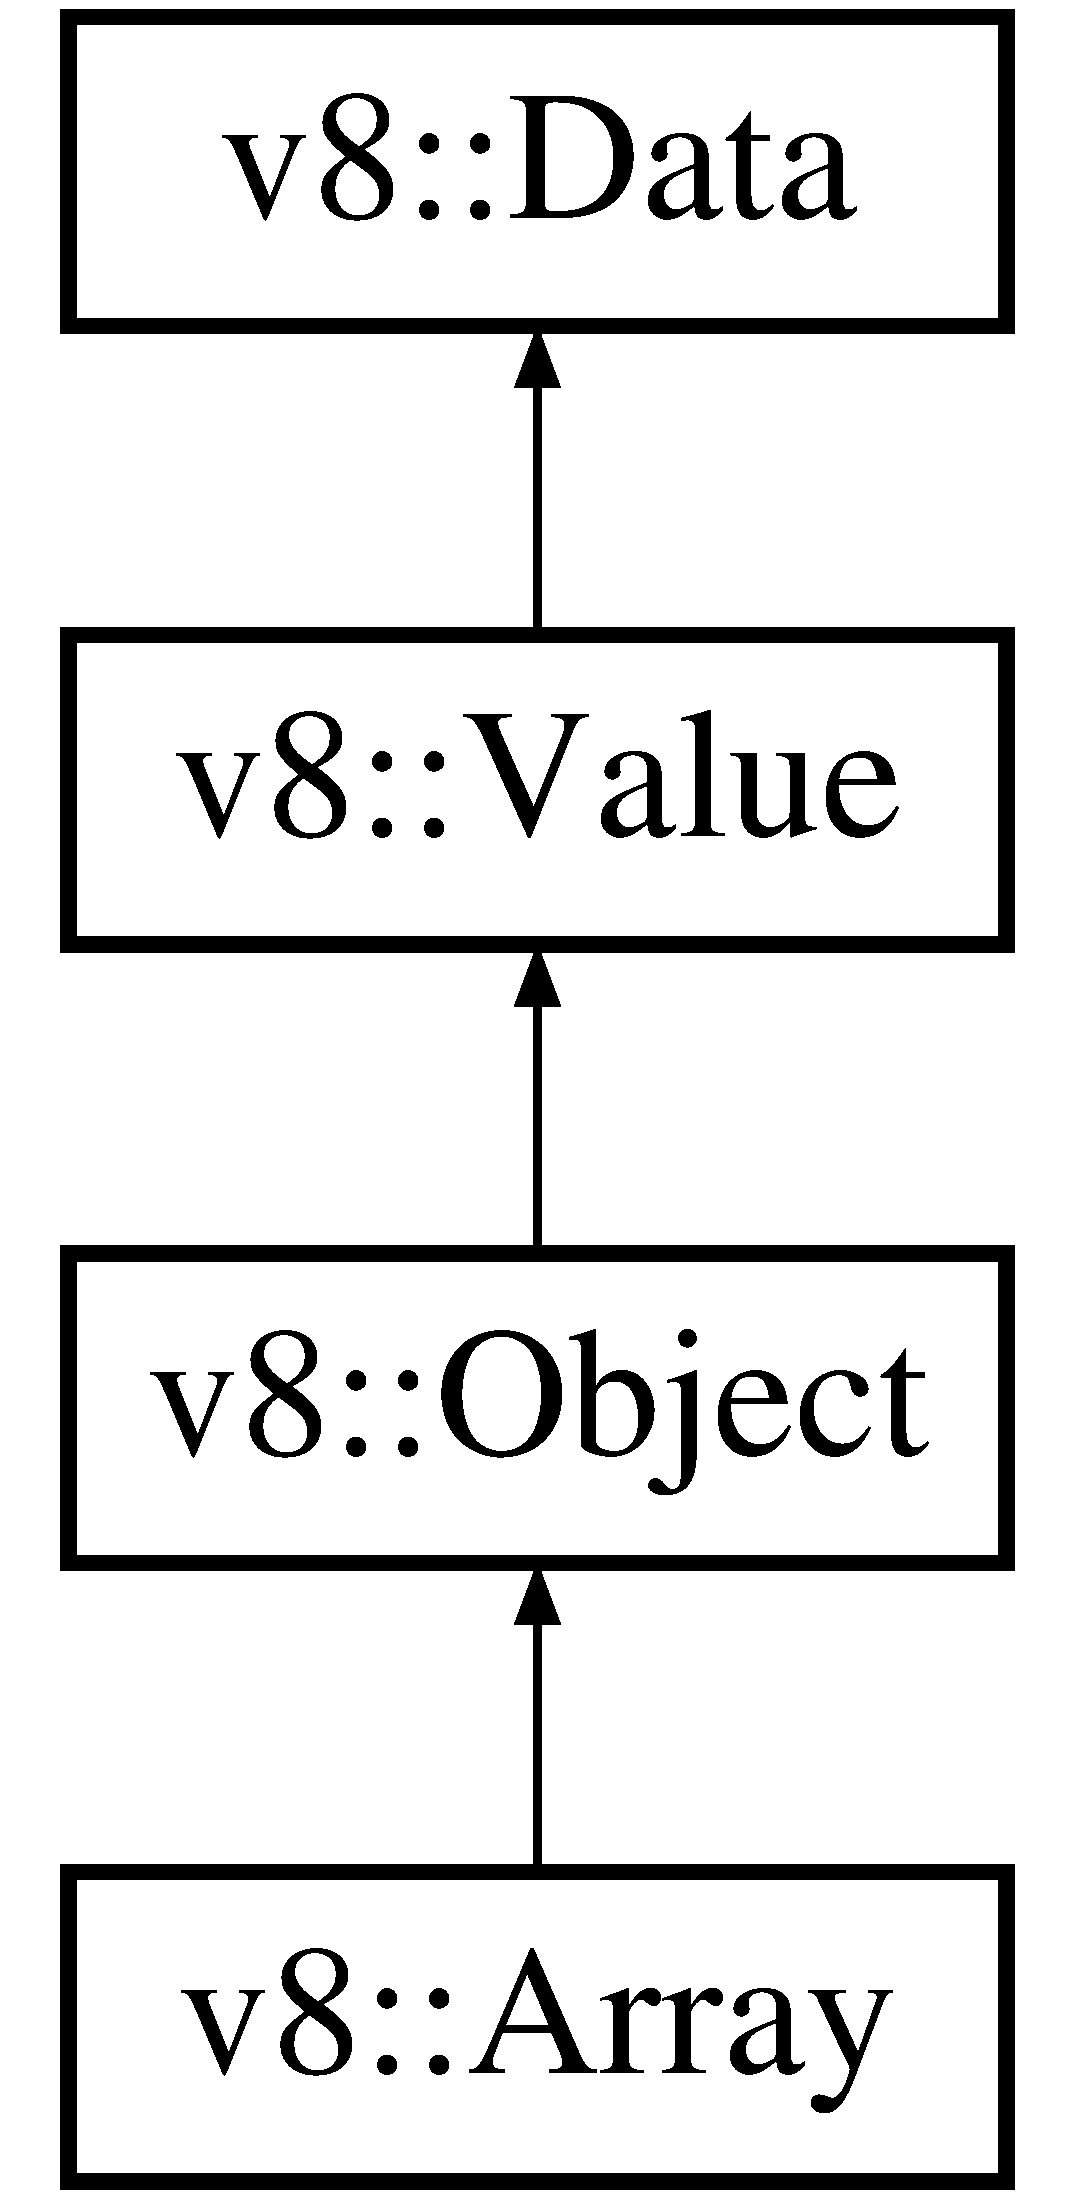
\includegraphics[height=4.000000cm]{classv8_1_1_array}
\end{center}
\end{figure}
\subsection*{Public Member Functions}
\begin{DoxyCompactItemize}
\item 
\hypertarget{classv8_1_1_array_a3e56e8707385ea9d6ca515ef7950670e}{}V8\+E\+X\+P\+O\+R\+T uint32\+\_\+t {\bfseries Length} () const \label{classv8_1_1_array_a3e56e8707385ea9d6ca515ef7950670e}

\item 
V8\+E\+X\+P\+O\+R\+T \hyperlink{classv8_1_1_local}{Local}$<$ \hyperlink{classv8_1_1_object}{Object} $>$ \hyperlink{classv8_1_1_array_ac78a0168b8612bcccd789497fd01b2ad}{Clone\+Element\+At} (uint32\+\_\+t index)
\end{DoxyCompactItemize}
\subsection*{Static Public Member Functions}
\begin{DoxyCompactItemize}
\item 
static V8\+E\+X\+P\+O\+R\+T \hyperlink{classv8_1_1_local}{Local}$<$ \hyperlink{classv8_1_1_array}{Array} $>$ \hyperlink{classv8_1_1_array_aabdb62437fce8c3769e69bbf44682066}{New} (int length=0)
\item 
\hypertarget{classv8_1_1_array_ae56792766f8513395c3ebe8c29afde4b}{}static \hyperlink{classv8_1_1_array}{Array} $\ast$ {\bfseries Cast} (\hyperlink{classv8_1_1_value}{Value} $\ast$obj)\label{classv8_1_1_array_ae56792766f8513395c3ebe8c29afde4b}

\end{DoxyCompactItemize}


\subsection{Detailed Description}
An instance of the built-\/in array constructor (E\+C\+M\+A-\/262, 15.\+4.\+2). 

\subsection{Member Function Documentation}
\hypertarget{classv8_1_1_array_ac78a0168b8612bcccd789497fd01b2ad}{}\index{v8\+::\+Array@{v8\+::\+Array}!Clone\+Element\+At@{Clone\+Element\+At}}
\index{Clone\+Element\+At@{Clone\+Element\+At}!v8\+::\+Array@{v8\+::\+Array}}
\subsubsection[{Clone\+Element\+At}]{\setlength{\rightskip}{0pt plus 5cm}V8\+E\+X\+P\+O\+R\+T {\bf Local}$<${\bf Object}$>$ v8\+::\+Array\+::\+Clone\+Element\+At (
\begin{DoxyParamCaption}
\item[{uint32\+\_\+t}]{index}
\end{DoxyParamCaption}
)}\label{classv8_1_1_array_ac78a0168b8612bcccd789497fd01b2ad}
Clones an element at index $\vert$index$\vert$. Returns an empty handle if cloning fails (for any reason). \hypertarget{classv8_1_1_array_aabdb62437fce8c3769e69bbf44682066}{}\index{v8\+::\+Array@{v8\+::\+Array}!New@{New}}
\index{New@{New}!v8\+::\+Array@{v8\+::\+Array}}
\subsubsection[{New}]{\setlength{\rightskip}{0pt plus 5cm}static V8\+E\+X\+P\+O\+R\+T {\bf Local}$<${\bf Array}$>$ v8\+::\+Array\+::\+New (
\begin{DoxyParamCaption}
\item[{int}]{length = {\ttfamily 0}}
\end{DoxyParamCaption}
)\hspace{0.3cm}{\ttfamily [static]}}\label{classv8_1_1_array_aabdb62437fce8c3769e69bbf44682066}
Creates a Java\+Script array with the given length. If the length is negative the returned array will have length 0. 

The documentation for this class was generated from the following file\+:\begin{DoxyCompactItemize}
\item 
deps/v8/include/v8.\+h\end{DoxyCompactItemize}

\hypertarget{classv8_1_1_string_1_1_ascii_value}{}\section{v8\+:\+:String\+:\+:Ascii\+Value Class Reference}
\label{classv8_1_1_string_1_1_ascii_value}\index{v8\+::\+String\+::\+Ascii\+Value@{v8\+::\+String\+::\+Ascii\+Value}}


{\ttfamily \#include $<$v8.\+h$>$}

\subsection*{Public Member Functions}
\begin{DoxyCompactItemize}
\item 
\hypertarget{classv8_1_1_string_1_1_ascii_value_a4e1559044a1e847517a9dcf6fca650d1}{}{\bfseries V8\+\_\+\+D\+E\+P\+R\+E\+C\+A\+T\+E\+D} (\char`\"{}Use \hyperlink{classv8_1_1_string_1_1_utf8_value}{Utf8\+Value} instead\char`\"{}, explicit \hyperlink{classv8_1_1_string_1_1_ascii_value}{Ascii\+Value}(\hyperlink{classv8_1_1_handle}{Handle}$<$ \hyperlink{classv8_1_1_value}{v8\+::\+Value} $>$ obj))\label{classv8_1_1_string_1_1_ascii_value_a4e1559044a1e847517a9dcf6fca650d1}

\item 
\hypertarget{classv8_1_1_string_1_1_ascii_value_a1e08f3a11aefee28cbbcbc386afd6032}{}char $\ast$ {\bfseries operator$\ast$} ()\label{classv8_1_1_string_1_1_ascii_value_a1e08f3a11aefee28cbbcbc386afd6032}

\item 
\hypertarget{classv8_1_1_string_1_1_ascii_value_abb007f038d674706da738f1f1f01f084}{}const char $\ast$ {\bfseries operator$\ast$} () const \label{classv8_1_1_string_1_1_ascii_value_abb007f038d674706da738f1f1f01f084}

\item 
\hypertarget{classv8_1_1_string_1_1_ascii_value_a97cccf0ed40a3deda1612c235b2f8068}{}int {\bfseries length} () const \label{classv8_1_1_string_1_1_ascii_value_a97cccf0ed40a3deda1612c235b2f8068}

\end{DoxyCompactItemize}


\subsection{Detailed Description}
Converts an object to an A\+S\+C\+I\+I string. Useful if you want to print the object. If conversion to a string fails (eg. due to an exception in the to\+String() method of the object) then the length() method returns 0 and the $\ast$ operator returns N\+U\+L\+L. 

The documentation for this class was generated from the following file\+:\begin{DoxyCompactItemize}
\item 
deps/v8/include/v8.\+h\end{DoxyCompactItemize}

\hypertarget{classv8_1_1_boolean}{}\section{v8\+:\+:Boolean Class Reference}
\label{classv8_1_1_boolean}\index{v8\+::\+Boolean@{v8\+::\+Boolean}}


{\ttfamily \#include $<$v8.\+h$>$}

Inheritance diagram for v8\+:\+:Boolean\+:\begin{figure}[H]
\begin{center}
\leavevmode
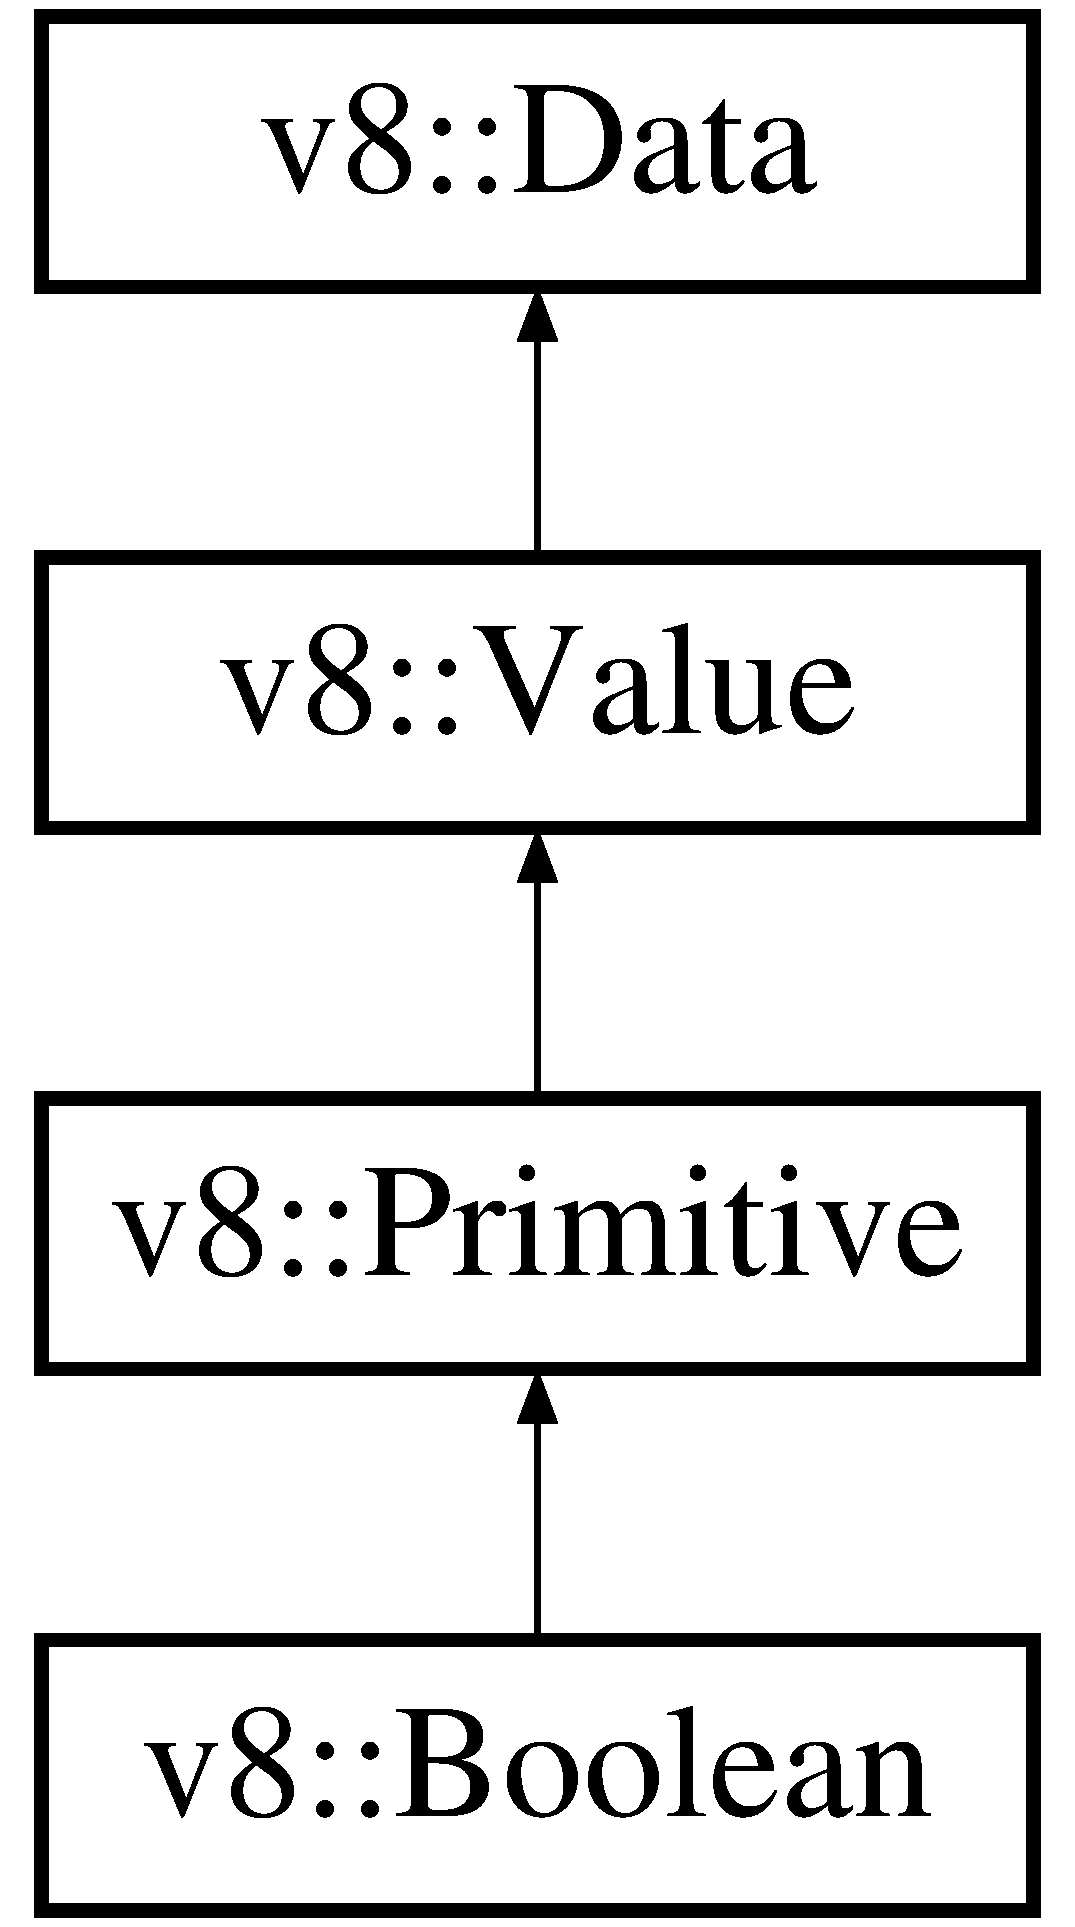
\includegraphics[height=4.000000cm]{classv8_1_1_boolean}
\end{center}
\end{figure}
\subsection*{Public Member Functions}
\begin{DoxyCompactItemize}
\item 
\hypertarget{classv8_1_1_boolean_aa493d54eb43afc64ab796e1cf66ff910}{}bool {\bfseries Value} () const \label{classv8_1_1_boolean_aa493d54eb43afc64ab796e1cf66ff910}

\end{DoxyCompactItemize}
\subsection*{Static Public Member Functions}
\begin{DoxyCompactItemize}
\item 
\hypertarget{classv8_1_1_boolean_ade49000b88ac4ae8ea3c13cf10067132}{}static \hyperlink{classv8_1_1_handle}{Handle}$<$ \hyperlink{classv8_1_1_boolean}{Boolean} $>$ {\bfseries New} (bool value)\label{classv8_1_1_boolean_ade49000b88ac4ae8ea3c13cf10067132}

\end{DoxyCompactItemize}


\subsection{Detailed Description}
A primitive boolean value (E\+C\+M\+A-\/262, 4.\+3.\+14). Either the true or false value. 

The documentation for this class was generated from the following file\+:\begin{DoxyCompactItemize}
\item 
deps/v8/include/v8.\+h\end{DoxyCompactItemize}

\hypertarget{classv8_1_1_debug_1_1_client_data}{}\section{v8\+:\+:Debug\+:\+:Client\+Data Class Reference}
\label{classv8_1_1_debug_1_1_client_data}\index{v8\+::\+Debug\+::\+Client\+Data@{v8\+::\+Debug\+::\+Client\+Data}}


{\ttfamily \#include $<$v8-\/debug.\+h$>$}



\subsection{Detailed Description}
A client object passed to the \hyperlink{namespacev8}{v8} debugger whose ownership will be taken by it. \hyperlink{namespacev8}{v8} is always responsible for deleting the object. 

The documentation for this class was generated from the following file\+:\begin{DoxyCompactItemize}
\item 
deps/v8/include/v8-\/debug.\+h\end{DoxyCompactItemize}

\hypertarget{classv8_1_1_context}{}\section{v8\+:\+:Context Class Reference}
\label{classv8_1_1_context}\index{v8\+::\+Context@{v8\+::\+Context}}


{\ttfamily \#include $<$v8.\+h$>$}

\subsection*{Classes}
\begin{DoxyCompactItemize}
\item 
class \hyperlink{classv8_1_1_context_1_1_scope}{Scope}
\end{DoxyCompactItemize}
\subsection*{Public Member Functions}
\begin{DoxyCompactItemize}
\item 
\hyperlink{classv8_1_1_local}{Local}$<$ \hyperlink{classv8_1_1_object}{Object} $>$ \hyperlink{classv8_1_1_context_af5cd9f97ef6a3307c1c21f80f4b743eb}{Global} ()
\item 
void \hyperlink{classv8_1_1_context_a841c7dd92eb8c57df92a268a164dea97}{Detach\+Global} ()
\item 
void \hyperlink{classv8_1_1_context_a1db9a514d7bb1c055a26359727bd2f6b}{Reattach\+Global} (\hyperlink{classv8_1_1_handle}{Handle}$<$ \hyperlink{classv8_1_1_object}{Object} $>$ global\+\_\+object)
\item 
void \hyperlink{classv8_1_1_context_a288d8549547f6bdf4312f5333f60f24d}{Set\+Security\+Token} (\hyperlink{classv8_1_1_handle}{Handle}$<$ \hyperlink{classv8_1_1_value}{Value} $>$ token)
\item 
void \hyperlink{classv8_1_1_context_aa9e1a14982b64fd51ab87600a287bad2}{Use\+Default\+Security\+Token} ()
\item 
\hyperlink{classv8_1_1_handle}{Handle}$<$ \hyperlink{classv8_1_1_value}{Value} $>$ \hyperlink{classv8_1_1_context_a8e71e658633518ca7718c0f6e938c6a9}{Get\+Security\+Token} ()
\item 
void \hyperlink{classv8_1_1_context_a6995c49d9897eb49053f07874b825133}{Enter} ()
\item 
void \hyperlink{classv8_1_1_context_a2db09d4fefb26023a40d88972a4c1599}{Exit} ()
\item 
bool \hyperlink{classv8_1_1_context_aadec400a5da1e79e58a8770fd706b9a0}{Has\+Out\+Of\+Memory\+Exception} ()
\item 
void \hyperlink{classv8_1_1_context_aaf39e5adc0ef4081d591952d17c6ada5}{Set\+Data} (\hyperlink{classv8_1_1_handle}{Handle}$<$ \hyperlink{classv8_1_1_string}{String} $>$ data)
\item 
\hypertarget{classv8_1_1_context_a0c5edad65549bf11edce29bfa3bc3aef}{}\hyperlink{classv8_1_1_local}{Local}$<$ \hyperlink{classv8_1_1_value}{Value} $>$ {\bfseries Get\+Data} ()\label{classv8_1_1_context_a0c5edad65549bf11edce29bfa3bc3aef}

\end{DoxyCompactItemize}
\subsection*{Static Public Member Functions}
\begin{DoxyCompactItemize}
\item 
static \hyperlink{classv8_1_1_persistent}{Persistent}$<$ \hyperlink{classv8_1_1_context}{Context} $>$ \hyperlink{classv8_1_1_context_add11dd18ee8e7f03d383afa79e87d1e6}{New} (\hyperlink{classv8_1_1_extension_configuration}{Extension\+Configuration} $\ast$extensions=N\+U\+L\+L, \hyperlink{classv8_1_1_handle}{Handle}$<$ \hyperlink{classv8_1_1_object_template}{Object\+Template} $>$ global\+\_\+template=\hyperlink{classv8_1_1_handle}{Handle}$<$ \hyperlink{classv8_1_1_object_template}{Object\+Template} $>$(), \hyperlink{classv8_1_1_handle}{Handle}$<$ \hyperlink{classv8_1_1_value}{Value} $>$ global\+\_\+object=\hyperlink{classv8_1_1_handle}{Handle}$<$ \hyperlink{classv8_1_1_value}{Value} $>$())
\item 
static \hyperlink{classv8_1_1_local}{Local}$<$ \hyperlink{classv8_1_1_context}{Context} $>$ \hyperlink{classv8_1_1_context_accfc7365efba8bce18cbf9df1c1fc79d}{Get\+Entered} ()
\item 
static \hyperlink{classv8_1_1_local}{Local}$<$ \hyperlink{classv8_1_1_context}{Context} $>$ \hyperlink{classv8_1_1_context_aca2df9d70e51f241d733f4ad0eb46401}{Get\+Current} ()
\item 
static \hyperlink{classv8_1_1_local}{Local}$<$ \hyperlink{classv8_1_1_context}{Context} $>$ \hyperlink{classv8_1_1_context_ad795cbbb842307a57d656dd9690fadf2}{Get\+Calling} ()
\item 
static bool \hyperlink{classv8_1_1_context_a5cf983417f9cfc6e1dd9228eccb78d31}{In\+Context} ()
\end{DoxyCompactItemize}
\subsection*{Friends}
\begin{DoxyCompactItemize}
\item 
\hypertarget{classv8_1_1_context_aeceedf6e1a7d48a588516ce2b1983d6f}{}class {\bfseries Value}\label{classv8_1_1_context_aeceedf6e1a7d48a588516ce2b1983d6f}

\item 
\hypertarget{classv8_1_1_context_ae98eaa96d1b24e087f3c3e372fb09dce}{}class {\bfseries Script}\label{classv8_1_1_context_ae98eaa96d1b24e087f3c3e372fb09dce}

\item 
\hypertarget{classv8_1_1_context_a0720b5f434e636e22a3ed34f847eec57}{}class {\bfseries Object}\label{classv8_1_1_context_a0720b5f434e636e22a3ed34f847eec57}

\item 
\hypertarget{classv8_1_1_context_ab7194606aa12931e96f8f5448d418ed0}{}class {\bfseries Function}\label{classv8_1_1_context_ab7194606aa12931e96f8f5448d418ed0}

\end{DoxyCompactItemize}


\subsection{Detailed Description}
A sandboxed execution context with its own set of built-\/in objects and functions. 

\subsection{Member Function Documentation}
\hypertarget{classv8_1_1_context_a841c7dd92eb8c57df92a268a164dea97}{}\index{v8\+::\+Context@{v8\+::\+Context}!Detach\+Global@{Detach\+Global}}
\index{Detach\+Global@{Detach\+Global}!v8\+::\+Context@{v8\+::\+Context}}
\subsubsection[{Detach\+Global}]{\setlength{\rightskip}{0pt plus 5cm}void v8\+::\+Context\+::\+Detach\+Global (
\begin{DoxyParamCaption}
{}
\end{DoxyParamCaption}
)}\label{classv8_1_1_context_a841c7dd92eb8c57df92a268a164dea97}
Detaches the global object from its context before the global object can be reused to create a new context. \hypertarget{classv8_1_1_context_a6995c49d9897eb49053f07874b825133}{}\index{v8\+::\+Context@{v8\+::\+Context}!Enter@{Enter}}
\index{Enter@{Enter}!v8\+::\+Context@{v8\+::\+Context}}
\subsubsection[{Enter}]{\setlength{\rightskip}{0pt plus 5cm}void v8\+::\+Context\+::\+Enter (
\begin{DoxyParamCaption}
{}
\end{DoxyParamCaption}
)}\label{classv8_1_1_context_a6995c49d9897eb49053f07874b825133}
Enter this context. After entering a context, all code compiled and run is compiled and run in this context. If another context is already entered, this old context is saved so it can be restored when the new context is exited. \hypertarget{classv8_1_1_context_a2db09d4fefb26023a40d88972a4c1599}{}\index{v8\+::\+Context@{v8\+::\+Context}!Exit@{Exit}}
\index{Exit@{Exit}!v8\+::\+Context@{v8\+::\+Context}}
\subsubsection[{Exit}]{\setlength{\rightskip}{0pt plus 5cm}void v8\+::\+Context\+::\+Exit (
\begin{DoxyParamCaption}
{}
\end{DoxyParamCaption}
)}\label{classv8_1_1_context_a2db09d4fefb26023a40d88972a4c1599}
Exit this context. Exiting the current context restores the context that was in place when entering the current context. \hypertarget{classv8_1_1_context_ad795cbbb842307a57d656dd9690fadf2}{}\index{v8\+::\+Context@{v8\+::\+Context}!Get\+Calling@{Get\+Calling}}
\index{Get\+Calling@{Get\+Calling}!v8\+::\+Context@{v8\+::\+Context}}
\subsubsection[{Get\+Calling}]{\setlength{\rightskip}{0pt plus 5cm}static {\bf Local}$<${\bf Context}$>$ v8\+::\+Context\+::\+Get\+Calling (
\begin{DoxyParamCaption}
{}
\end{DoxyParamCaption}
)\hspace{0.3cm}{\ttfamily [static]}}\label{classv8_1_1_context_ad795cbbb842307a57d656dd9690fadf2}
Returns the context of the calling Java\+Script code. That is the context of the top-\/most Java\+Script frame. If there are no Java\+Script frames an empty handle is returned. \hypertarget{classv8_1_1_context_aca2df9d70e51f241d733f4ad0eb46401}{}\index{v8\+::\+Context@{v8\+::\+Context}!Get\+Current@{Get\+Current}}
\index{Get\+Current@{Get\+Current}!v8\+::\+Context@{v8\+::\+Context}}
\subsubsection[{Get\+Current}]{\setlength{\rightskip}{0pt plus 5cm}static {\bf Local}$<${\bf Context}$>$ v8\+::\+Context\+::\+Get\+Current (
\begin{DoxyParamCaption}
{}
\end{DoxyParamCaption}
)\hspace{0.3cm}{\ttfamily [static]}}\label{classv8_1_1_context_aca2df9d70e51f241d733f4ad0eb46401}
Returns the context that is on the top of the stack. \hypertarget{classv8_1_1_context_accfc7365efba8bce18cbf9df1c1fc79d}{}\index{v8\+::\+Context@{v8\+::\+Context}!Get\+Entered@{Get\+Entered}}
\index{Get\+Entered@{Get\+Entered}!v8\+::\+Context@{v8\+::\+Context}}
\subsubsection[{Get\+Entered}]{\setlength{\rightskip}{0pt plus 5cm}static {\bf Local}$<${\bf Context}$>$ v8\+::\+Context\+::\+Get\+Entered (
\begin{DoxyParamCaption}
{}
\end{DoxyParamCaption}
)\hspace{0.3cm}{\ttfamily [static]}}\label{classv8_1_1_context_accfc7365efba8bce18cbf9df1c1fc79d}
Returns the last entered context. \hypertarget{classv8_1_1_context_a8e71e658633518ca7718c0f6e938c6a9}{}\index{v8\+::\+Context@{v8\+::\+Context}!Get\+Security\+Token@{Get\+Security\+Token}}
\index{Get\+Security\+Token@{Get\+Security\+Token}!v8\+::\+Context@{v8\+::\+Context}}
\subsubsection[{Get\+Security\+Token}]{\setlength{\rightskip}{0pt plus 5cm}{\bf Handle}$<${\bf Value}$>$ v8\+::\+Context\+::\+Get\+Security\+Token (
\begin{DoxyParamCaption}
{}
\end{DoxyParamCaption}
)}\label{classv8_1_1_context_a8e71e658633518ca7718c0f6e938c6a9}
Returns the security token of this context. \hypertarget{classv8_1_1_context_af5cd9f97ef6a3307c1c21f80f4b743eb}{}\index{v8\+::\+Context@{v8\+::\+Context}!Global@{Global}}
\index{Global@{Global}!v8\+::\+Context@{v8\+::\+Context}}
\subsubsection[{Global}]{\setlength{\rightskip}{0pt plus 5cm}{\bf Local}$<${\bf Object}$>$ v8\+::\+Context\+::\+Global (
\begin{DoxyParamCaption}
{}
\end{DoxyParamCaption}
)}\label{classv8_1_1_context_af5cd9f97ef6a3307c1c21f80f4b743eb}
Returns the global object of the context. \hypertarget{classv8_1_1_context_aadec400a5da1e79e58a8770fd706b9a0}{}\index{v8\+::\+Context@{v8\+::\+Context}!Has\+Out\+Of\+Memory\+Exception@{Has\+Out\+Of\+Memory\+Exception}}
\index{Has\+Out\+Of\+Memory\+Exception@{Has\+Out\+Of\+Memory\+Exception}!v8\+::\+Context@{v8\+::\+Context}}
\subsubsection[{Has\+Out\+Of\+Memory\+Exception}]{\setlength{\rightskip}{0pt plus 5cm}bool v8\+::\+Context\+::\+Has\+Out\+Of\+Memory\+Exception (
\begin{DoxyParamCaption}
{}
\end{DoxyParamCaption}
)}\label{classv8_1_1_context_aadec400a5da1e79e58a8770fd706b9a0}
Returns true if the context has experienced an out of memory situation. \hypertarget{classv8_1_1_context_a5cf983417f9cfc6e1dd9228eccb78d31}{}\index{v8\+::\+Context@{v8\+::\+Context}!In\+Context@{In\+Context}}
\index{In\+Context@{In\+Context}!v8\+::\+Context@{v8\+::\+Context}}
\subsubsection[{In\+Context}]{\setlength{\rightskip}{0pt plus 5cm}static bool v8\+::\+Context\+::\+In\+Context (
\begin{DoxyParamCaption}
{}
\end{DoxyParamCaption}
)\hspace{0.3cm}{\ttfamily [static]}}\label{classv8_1_1_context_a5cf983417f9cfc6e1dd9228eccb78d31}
Returns true if \hyperlink{classv8_1_1_v8}{V8} has a current context. \hypertarget{classv8_1_1_context_add11dd18ee8e7f03d383afa79e87d1e6}{}\index{v8\+::\+Context@{v8\+::\+Context}!New@{New}}
\index{New@{New}!v8\+::\+Context@{v8\+::\+Context}}
\subsubsection[{New}]{\setlength{\rightskip}{0pt plus 5cm}static {\bf Persistent}$<${\bf Context}$>$ v8\+::\+Context\+::\+New (
\begin{DoxyParamCaption}
\item[{{\bf Extension\+Configuration} $\ast$}]{extensions = {\ttfamily NULL}, }
\item[{{\bf Handle}$<$ {\bf Object\+Template} $>$}]{global\+\_\+template = {\ttfamily {\bf Handle}$<$~{\bf Object\+Template}~$>$()}, }
\item[{{\bf Handle}$<$ {\bf Value} $>$}]{global\+\_\+object = {\ttfamily {\bf Handle}$<$~{\bf Value}~$>$()}}
\end{DoxyParamCaption}
)\hspace{0.3cm}{\ttfamily [static]}}\label{classv8_1_1_context_add11dd18ee8e7f03d383afa79e87d1e6}
Creates a new context.

Returns a persistent handle to the newly allocated context. This persistent handle has to be disposed when the context is no longer used so the context can be garbage collected.


\begin{DoxyParams}{Parameters}
{\em extensions} & An optional extension configuration containing the extensions to be installed in the newly created context.\\
\hline
{\em global\+\_\+template} & An optional object template from which the global object for the newly created context will be created.\\
\hline
{\em global\+\_\+object} & An optional global object to be reused for the newly created context. This global object must have been created by a previous call to \hyperlink{classv8_1_1_context_add11dd18ee8e7f03d383afa79e87d1e6}{Context\+::\+New} with the same global template. The state of the global object will be completely reset and only object identify will remain. \\
\hline
\end{DoxyParams}
\hypertarget{classv8_1_1_context_a1db9a514d7bb1c055a26359727bd2f6b}{}\index{v8\+::\+Context@{v8\+::\+Context}!Reattach\+Global@{Reattach\+Global}}
\index{Reattach\+Global@{Reattach\+Global}!v8\+::\+Context@{v8\+::\+Context}}
\subsubsection[{Reattach\+Global}]{\setlength{\rightskip}{0pt plus 5cm}void v8\+::\+Context\+::\+Reattach\+Global (
\begin{DoxyParamCaption}
\item[{{\bf Handle}$<$ {\bf Object} $>$}]{global\+\_\+object}
\end{DoxyParamCaption}
)}\label{classv8_1_1_context_a1db9a514d7bb1c055a26359727bd2f6b}
Reattaches a global object to a context. This can be used to restore the connection between a global object and a context after Detach\+Global has been called.


\begin{DoxyParams}{Parameters}
{\em global\+\_\+object} & The global object to reattach to the context. For this to work, the global object must be the global object that was associated with this context before a call to Detach\+Global. \\
\hline
\end{DoxyParams}
\hypertarget{classv8_1_1_context_aaf39e5adc0ef4081d591952d17c6ada5}{}\index{v8\+::\+Context@{v8\+::\+Context}!Set\+Data@{Set\+Data}}
\index{Set\+Data@{Set\+Data}!v8\+::\+Context@{v8\+::\+Context}}
\subsubsection[{Set\+Data}]{\setlength{\rightskip}{0pt plus 5cm}void v8\+::\+Context\+::\+Set\+Data (
\begin{DoxyParamCaption}
\item[{{\bf Handle}$<$ {\bf String} $>$}]{data}
\end{DoxyParamCaption}
)}\label{classv8_1_1_context_aaf39e5adc0ef4081d591952d17c6ada5}
Associate an additional data object with the context. This is mainly used with the debugger to provide additional information on the context through the debugger A\+P\+I. \hypertarget{classv8_1_1_context_a288d8549547f6bdf4312f5333f60f24d}{}\index{v8\+::\+Context@{v8\+::\+Context}!Set\+Security\+Token@{Set\+Security\+Token}}
\index{Set\+Security\+Token@{Set\+Security\+Token}!v8\+::\+Context@{v8\+::\+Context}}
\subsubsection[{Set\+Security\+Token}]{\setlength{\rightskip}{0pt plus 5cm}void v8\+::\+Context\+::\+Set\+Security\+Token (
\begin{DoxyParamCaption}
\item[{{\bf Handle}$<$ {\bf Value} $>$}]{token}
\end{DoxyParamCaption}
)}\label{classv8_1_1_context_a288d8549547f6bdf4312f5333f60f24d}
Sets the security token for the context. To access an object in another context, the security tokens must match. \hypertarget{classv8_1_1_context_aa9e1a14982b64fd51ab87600a287bad2}{}\index{v8\+::\+Context@{v8\+::\+Context}!Use\+Default\+Security\+Token@{Use\+Default\+Security\+Token}}
\index{Use\+Default\+Security\+Token@{Use\+Default\+Security\+Token}!v8\+::\+Context@{v8\+::\+Context}}
\subsubsection[{Use\+Default\+Security\+Token}]{\setlength{\rightskip}{0pt plus 5cm}void v8\+::\+Context\+::\+Use\+Default\+Security\+Token (
\begin{DoxyParamCaption}
{}
\end{DoxyParamCaption}
)}\label{classv8_1_1_context_aa9e1a14982b64fd51ab87600a287bad2}
Restores the security token to the default value. 

The documentation for this class was generated from the following file\+:\begin{DoxyCompactItemize}
\item 
deps/v8/include/v8.\+h\end{DoxyCompactItemize}

\hypertarget{classv8_1_1_cpu_profile}{}\section{v8\+:\+:Cpu\+Profile Class Reference}
\label{classv8_1_1_cpu_profile}\index{v8\+::\+Cpu\+Profile@{v8\+::\+Cpu\+Profile}}


{\ttfamily \#include $<$v8-\/profiler.\+h$>$}

\subsection*{Public Member Functions}
\begin{DoxyCompactItemize}
\item 
\hyperlink{classv8_1_1_handle}{Handle}$<$ \hyperlink{classv8_1_1_string}{String} $>$ \hyperlink{classv8_1_1_cpu_profile_afbb44d5cf0a8729c9074aba03207e5cc}{Get\+Title} () const 
\item 
const \hyperlink{classv8_1_1_cpu_profile_node}{Cpu\+Profile\+Node} $\ast$ \hyperlink{classv8_1_1_cpu_profile_aec978f073af6634b6495baa65209a31f}{Get\+Top\+Down\+Root} () const 
\item 
int \hyperlink{classv8_1_1_cpu_profile_a2ca9d8e862dc2b06892196b5e5a14994}{Get\+Samples\+Count} () const 
\item 
const \hyperlink{classv8_1_1_cpu_profile_node}{Cpu\+Profile\+Node} $\ast$ \hyperlink{classv8_1_1_cpu_profile_a59470cd1286e949dd069eea87777a074}{Get\+Sample} (int index) const 
\item 
int64\+\_\+t \hyperlink{classv8_1_1_cpu_profile_aac317de54bdfc4523b5ecea522c01ad1}{Get\+Start\+Time} () const 
\item 
int64\+\_\+t \hyperlink{classv8_1_1_cpu_profile_a15170e2e9eeb972fddf949bd08dd09ff}{Get\+End\+Time} () const 
\item 
void \hyperlink{classv8_1_1_cpu_profile_a70c93f0c14d07a7e1bad42ee95665ca0}{Delete} ()
\end{DoxyCompactItemize}


\subsection{Detailed Description}
\hyperlink{classv8_1_1_cpu_profile}{Cpu\+Profile} contains a C\+P\+U profile in a form of top-\/down call tree (from main() down to functions that do all the work). 

\subsection{Member Function Documentation}
\hypertarget{classv8_1_1_cpu_profile_a70c93f0c14d07a7e1bad42ee95665ca0}{}\index{v8\+::\+Cpu\+Profile@{v8\+::\+Cpu\+Profile}!Delete@{Delete}}
\index{Delete@{Delete}!v8\+::\+Cpu\+Profile@{v8\+::\+Cpu\+Profile}}
\subsubsection[{Delete}]{\setlength{\rightskip}{0pt plus 5cm}void v8\+::\+Cpu\+Profile\+::\+Delete (
\begin{DoxyParamCaption}
{}
\end{DoxyParamCaption}
)}\label{classv8_1_1_cpu_profile_a70c93f0c14d07a7e1bad42ee95665ca0}
Deletes the profile and removes it from \hyperlink{classv8_1_1_cpu_profiler}{Cpu\+Profiler}\textquotesingle{}s list. All pointers to nodes previously returned become invalid. \hypertarget{classv8_1_1_cpu_profile_a15170e2e9eeb972fddf949bd08dd09ff}{}\index{v8\+::\+Cpu\+Profile@{v8\+::\+Cpu\+Profile}!Get\+End\+Time@{Get\+End\+Time}}
\index{Get\+End\+Time@{Get\+End\+Time}!v8\+::\+Cpu\+Profile@{v8\+::\+Cpu\+Profile}}
\subsubsection[{Get\+End\+Time}]{\setlength{\rightskip}{0pt plus 5cm}int64\+\_\+t v8\+::\+Cpu\+Profile\+::\+Get\+End\+Time (
\begin{DoxyParamCaption}
{}
\end{DoxyParamCaption}
) const}\label{classv8_1_1_cpu_profile_a15170e2e9eeb972fddf949bd08dd09ff}
Returns time when the profile recording was stopped (in microseconds since the Epoch). \hypertarget{classv8_1_1_cpu_profile_a59470cd1286e949dd069eea87777a074}{}\index{v8\+::\+Cpu\+Profile@{v8\+::\+Cpu\+Profile}!Get\+Sample@{Get\+Sample}}
\index{Get\+Sample@{Get\+Sample}!v8\+::\+Cpu\+Profile@{v8\+::\+Cpu\+Profile}}
\subsubsection[{Get\+Sample}]{\setlength{\rightskip}{0pt plus 5cm}const {\bf Cpu\+Profile\+Node}$\ast$ v8\+::\+Cpu\+Profile\+::\+Get\+Sample (
\begin{DoxyParamCaption}
\item[{int}]{index}
\end{DoxyParamCaption}
) const}\label{classv8_1_1_cpu_profile_a59470cd1286e949dd069eea87777a074}
Returns profile node corresponding to the top frame the sample at the given index. \hypertarget{classv8_1_1_cpu_profile_a2ca9d8e862dc2b06892196b5e5a14994}{}\index{v8\+::\+Cpu\+Profile@{v8\+::\+Cpu\+Profile}!Get\+Samples\+Count@{Get\+Samples\+Count}}
\index{Get\+Samples\+Count@{Get\+Samples\+Count}!v8\+::\+Cpu\+Profile@{v8\+::\+Cpu\+Profile}}
\subsubsection[{Get\+Samples\+Count}]{\setlength{\rightskip}{0pt plus 5cm}int v8\+::\+Cpu\+Profile\+::\+Get\+Samples\+Count (
\begin{DoxyParamCaption}
{}
\end{DoxyParamCaption}
) const}\label{classv8_1_1_cpu_profile_a2ca9d8e862dc2b06892196b5e5a14994}
Returns number of samples recorded. The samples are not recorded unless $\vert$record\+\_\+samples$\vert$ parameter of \hyperlink{classv8_1_1_cpu_profiler_a61b2b49010708f0283c1613e2bdc1adc}{Cpu\+Profiler\+::\+Start\+Cpu\+Profiling} is true. \hypertarget{classv8_1_1_cpu_profile_aac317de54bdfc4523b5ecea522c01ad1}{}\index{v8\+::\+Cpu\+Profile@{v8\+::\+Cpu\+Profile}!Get\+Start\+Time@{Get\+Start\+Time}}
\index{Get\+Start\+Time@{Get\+Start\+Time}!v8\+::\+Cpu\+Profile@{v8\+::\+Cpu\+Profile}}
\subsubsection[{Get\+Start\+Time}]{\setlength{\rightskip}{0pt plus 5cm}int64\+\_\+t v8\+::\+Cpu\+Profile\+::\+Get\+Start\+Time (
\begin{DoxyParamCaption}
{}
\end{DoxyParamCaption}
) const}\label{classv8_1_1_cpu_profile_aac317de54bdfc4523b5ecea522c01ad1}
Returns time when the profile recording started (in microseconds since the Epoch). \hypertarget{classv8_1_1_cpu_profile_afbb44d5cf0a8729c9074aba03207e5cc}{}\index{v8\+::\+Cpu\+Profile@{v8\+::\+Cpu\+Profile}!Get\+Title@{Get\+Title}}
\index{Get\+Title@{Get\+Title}!v8\+::\+Cpu\+Profile@{v8\+::\+Cpu\+Profile}}
\subsubsection[{Get\+Title}]{\setlength{\rightskip}{0pt plus 5cm}{\bf Handle}$<${\bf String}$>$ v8\+::\+Cpu\+Profile\+::\+Get\+Title (
\begin{DoxyParamCaption}
{}
\end{DoxyParamCaption}
) const}\label{classv8_1_1_cpu_profile_afbb44d5cf0a8729c9074aba03207e5cc}
Returns C\+P\+U profile title. \hypertarget{classv8_1_1_cpu_profile_aec978f073af6634b6495baa65209a31f}{}\index{v8\+::\+Cpu\+Profile@{v8\+::\+Cpu\+Profile}!Get\+Top\+Down\+Root@{Get\+Top\+Down\+Root}}
\index{Get\+Top\+Down\+Root@{Get\+Top\+Down\+Root}!v8\+::\+Cpu\+Profile@{v8\+::\+Cpu\+Profile}}
\subsubsection[{Get\+Top\+Down\+Root}]{\setlength{\rightskip}{0pt plus 5cm}const {\bf Cpu\+Profile\+Node}$\ast$ v8\+::\+Cpu\+Profile\+::\+Get\+Top\+Down\+Root (
\begin{DoxyParamCaption}
{}
\end{DoxyParamCaption}
) const}\label{classv8_1_1_cpu_profile_aec978f073af6634b6495baa65209a31f}
Returns the root node of the top down call tree. 

The documentation for this class was generated from the following file\+:\begin{DoxyCompactItemize}
\item 
deps/v8/include/v8-\/profiler.\+h\end{DoxyCompactItemize}

\hypertarget{classv8_1_1_cpu_profile_node}{}\section{v8\+:\+:Cpu\+Profile\+Node Class Reference}
\label{classv8_1_1_cpu_profile_node}\index{v8\+::\+Cpu\+Profile\+Node@{v8\+::\+Cpu\+Profile\+Node}}


{\ttfamily \#include $<$v8-\/profiler.\+h$>$}

\subsection*{Public Member Functions}
\begin{DoxyCompactItemize}
\item 
\hyperlink{classv8_1_1_handle}{Handle}$<$ \hyperlink{classv8_1_1_string}{String} $>$ \hyperlink{classv8_1_1_cpu_profile_node_affbc7842b66986012285602ab65aa5f8}{Get\+Function\+Name} () const 
\item 
\hyperlink{classv8_1_1_handle}{Handle}$<$ \hyperlink{classv8_1_1_string}{String} $>$ \hyperlink{classv8_1_1_cpu_profile_node_a140dd536e7096701a36be0083c18c268}{Get\+Script\+Resource\+Name} () const 
\item 
int \hyperlink{classv8_1_1_cpu_profile_node_a45ea035661c7152e4f3eb47f73787a75}{Get\+Line\+Number} () const 
\item 
double \hyperlink{classv8_1_1_cpu_profile_node_a49f16893b9f9c94c58ea845fb039330a}{Get\+Total\+Time} () const 
\item 
double \hyperlink{classv8_1_1_cpu_profile_node_aa2e4d36f22f49726715ed36fef5a23b6}{Get\+Self\+Time} () const 
\item 
double \hyperlink{classv8_1_1_cpu_profile_node_a0e719d2013377f03583342c28fb5cb27}{Get\+Total\+Samples\+Count} () const 
\item 
double \hyperlink{classv8_1_1_cpu_profile_node_a78537aa4471d6c1ebc37993f711090db}{Get\+Self\+Samples\+Count} () const 
\item 
unsigned \hyperlink{classv8_1_1_cpu_profile_node_a245092eb223b948fc9441664d9e2701e}{Get\+Call\+Uid} () const 
\item 
unsigned \hyperlink{classv8_1_1_cpu_profile_node_ae2971c5003353a984ef72b6cddf5e298}{Get\+Node\+Id} () const 
\item 
int \hyperlink{classv8_1_1_cpu_profile_node_ac4612b91e43a2901ac20c3705288955b}{Get\+Children\+Count} () const 
\item 
const \hyperlink{classv8_1_1_cpu_profile_node}{Cpu\+Profile\+Node} $\ast$ \hyperlink{classv8_1_1_cpu_profile_node_aa397db1e0f5147155164c5ea3e854d69}{Get\+Child} (int index) const 
\end{DoxyCompactItemize}
\subsection*{Static Public Attributes}
\begin{DoxyCompactItemize}
\item 
\hypertarget{classv8_1_1_cpu_profile_node_ad54213fe8a795cb6669566f0272fc5ba}{}static const int {\bfseries k\+No\+Line\+Number\+Info} = Message\+::k\+No\+Line\+Number\+Info\label{classv8_1_1_cpu_profile_node_ad54213fe8a795cb6669566f0272fc5ba}

\end{DoxyCompactItemize}


\subsection{Detailed Description}
\hyperlink{classv8_1_1_cpu_profile_node}{Cpu\+Profile\+Node} represents a node in a call graph. 

\subsection{Member Function Documentation}
\hypertarget{classv8_1_1_cpu_profile_node_a245092eb223b948fc9441664d9e2701e}{}\index{v8\+::\+Cpu\+Profile\+Node@{v8\+::\+Cpu\+Profile\+Node}!Get\+Call\+Uid@{Get\+Call\+Uid}}
\index{Get\+Call\+Uid@{Get\+Call\+Uid}!v8\+::\+Cpu\+Profile\+Node@{v8\+::\+Cpu\+Profile\+Node}}
\subsubsection[{Get\+Call\+Uid}]{\setlength{\rightskip}{0pt plus 5cm}unsigned v8\+::\+Cpu\+Profile\+Node\+::\+Get\+Call\+Uid (
\begin{DoxyParamCaption}
{}
\end{DoxyParamCaption}
) const}\label{classv8_1_1_cpu_profile_node_a245092eb223b948fc9441664d9e2701e}
Returns function entry U\+I\+D. \hypertarget{classv8_1_1_cpu_profile_node_aa397db1e0f5147155164c5ea3e854d69}{}\index{v8\+::\+Cpu\+Profile\+Node@{v8\+::\+Cpu\+Profile\+Node}!Get\+Child@{Get\+Child}}
\index{Get\+Child@{Get\+Child}!v8\+::\+Cpu\+Profile\+Node@{v8\+::\+Cpu\+Profile\+Node}}
\subsubsection[{Get\+Child}]{\setlength{\rightskip}{0pt plus 5cm}const {\bf Cpu\+Profile\+Node}$\ast$ v8\+::\+Cpu\+Profile\+Node\+::\+Get\+Child (
\begin{DoxyParamCaption}
\item[{int}]{index}
\end{DoxyParamCaption}
) const}\label{classv8_1_1_cpu_profile_node_aa397db1e0f5147155164c5ea3e854d69}
Retrieves a child node by index. \hypertarget{classv8_1_1_cpu_profile_node_ac4612b91e43a2901ac20c3705288955b}{}\index{v8\+::\+Cpu\+Profile\+Node@{v8\+::\+Cpu\+Profile\+Node}!Get\+Children\+Count@{Get\+Children\+Count}}
\index{Get\+Children\+Count@{Get\+Children\+Count}!v8\+::\+Cpu\+Profile\+Node@{v8\+::\+Cpu\+Profile\+Node}}
\subsubsection[{Get\+Children\+Count}]{\setlength{\rightskip}{0pt plus 5cm}int v8\+::\+Cpu\+Profile\+Node\+::\+Get\+Children\+Count (
\begin{DoxyParamCaption}
{}
\end{DoxyParamCaption}
) const}\label{classv8_1_1_cpu_profile_node_ac4612b91e43a2901ac20c3705288955b}
Returns child nodes count of the node. \hypertarget{classv8_1_1_cpu_profile_node_affbc7842b66986012285602ab65aa5f8}{}\index{v8\+::\+Cpu\+Profile\+Node@{v8\+::\+Cpu\+Profile\+Node}!Get\+Function\+Name@{Get\+Function\+Name}}
\index{Get\+Function\+Name@{Get\+Function\+Name}!v8\+::\+Cpu\+Profile\+Node@{v8\+::\+Cpu\+Profile\+Node}}
\subsubsection[{Get\+Function\+Name}]{\setlength{\rightskip}{0pt plus 5cm}{\bf Handle}$<${\bf String}$>$ v8\+::\+Cpu\+Profile\+Node\+::\+Get\+Function\+Name (
\begin{DoxyParamCaption}
{}
\end{DoxyParamCaption}
) const}\label{classv8_1_1_cpu_profile_node_affbc7842b66986012285602ab65aa5f8}
Returns function name (empty string for anonymous functions.) \hypertarget{classv8_1_1_cpu_profile_node_a45ea035661c7152e4f3eb47f73787a75}{}\index{v8\+::\+Cpu\+Profile\+Node@{v8\+::\+Cpu\+Profile\+Node}!Get\+Line\+Number@{Get\+Line\+Number}}
\index{Get\+Line\+Number@{Get\+Line\+Number}!v8\+::\+Cpu\+Profile\+Node@{v8\+::\+Cpu\+Profile\+Node}}
\subsubsection[{Get\+Line\+Number}]{\setlength{\rightskip}{0pt plus 5cm}int v8\+::\+Cpu\+Profile\+Node\+::\+Get\+Line\+Number (
\begin{DoxyParamCaption}
{}
\end{DoxyParamCaption}
) const}\label{classv8_1_1_cpu_profile_node_a45ea035661c7152e4f3eb47f73787a75}
Returns the number, 1-\/based, of the line where the function originates. k\+No\+Line\+Number\+Info if no line number information is available. \hypertarget{classv8_1_1_cpu_profile_node_ae2971c5003353a984ef72b6cddf5e298}{}\index{v8\+::\+Cpu\+Profile\+Node@{v8\+::\+Cpu\+Profile\+Node}!Get\+Node\+Id@{Get\+Node\+Id}}
\index{Get\+Node\+Id@{Get\+Node\+Id}!v8\+::\+Cpu\+Profile\+Node@{v8\+::\+Cpu\+Profile\+Node}}
\subsubsection[{Get\+Node\+Id}]{\setlength{\rightskip}{0pt plus 5cm}unsigned v8\+::\+Cpu\+Profile\+Node\+::\+Get\+Node\+Id (
\begin{DoxyParamCaption}
{}
\end{DoxyParamCaption}
) const}\label{classv8_1_1_cpu_profile_node_ae2971c5003353a984ef72b6cddf5e298}
Returns id of the node. The id is unique within the tree \hypertarget{classv8_1_1_cpu_profile_node_a140dd536e7096701a36be0083c18c268}{}\index{v8\+::\+Cpu\+Profile\+Node@{v8\+::\+Cpu\+Profile\+Node}!Get\+Script\+Resource\+Name@{Get\+Script\+Resource\+Name}}
\index{Get\+Script\+Resource\+Name@{Get\+Script\+Resource\+Name}!v8\+::\+Cpu\+Profile\+Node@{v8\+::\+Cpu\+Profile\+Node}}
\subsubsection[{Get\+Script\+Resource\+Name}]{\setlength{\rightskip}{0pt plus 5cm}{\bf Handle}$<${\bf String}$>$ v8\+::\+Cpu\+Profile\+Node\+::\+Get\+Script\+Resource\+Name (
\begin{DoxyParamCaption}
{}
\end{DoxyParamCaption}
) const}\label{classv8_1_1_cpu_profile_node_a140dd536e7096701a36be0083c18c268}
Returns resource name for script from where the function originates. \hypertarget{classv8_1_1_cpu_profile_node_a78537aa4471d6c1ebc37993f711090db}{}\index{v8\+::\+Cpu\+Profile\+Node@{v8\+::\+Cpu\+Profile\+Node}!Get\+Self\+Samples\+Count@{Get\+Self\+Samples\+Count}}
\index{Get\+Self\+Samples\+Count@{Get\+Self\+Samples\+Count}!v8\+::\+Cpu\+Profile\+Node@{v8\+::\+Cpu\+Profile\+Node}}
\subsubsection[{Get\+Self\+Samples\+Count}]{\setlength{\rightskip}{0pt plus 5cm}double v8\+::\+Cpu\+Profile\+Node\+::\+Get\+Self\+Samples\+Count (
\begin{DoxyParamCaption}
{}
\end{DoxyParamCaption}
) const}\label{classv8_1_1_cpu_profile_node_a78537aa4471d6c1ebc37993f711090db}
Returns the count of samples where function was currently executing. \hypertarget{classv8_1_1_cpu_profile_node_aa2e4d36f22f49726715ed36fef5a23b6}{}\index{v8\+::\+Cpu\+Profile\+Node@{v8\+::\+Cpu\+Profile\+Node}!Get\+Self\+Time@{Get\+Self\+Time}}
\index{Get\+Self\+Time@{Get\+Self\+Time}!v8\+::\+Cpu\+Profile\+Node@{v8\+::\+Cpu\+Profile\+Node}}
\subsubsection[{Get\+Self\+Time}]{\setlength{\rightskip}{0pt plus 5cm}double v8\+::\+Cpu\+Profile\+Node\+::\+Get\+Self\+Time (
\begin{DoxyParamCaption}
{}
\end{DoxyParamCaption}
) const}\label{classv8_1_1_cpu_profile_node_aa2e4d36f22f49726715ed36fef5a23b6}
Returns self execution time of the function, in milliseconds, estimated by samples count. \hypertarget{classv8_1_1_cpu_profile_node_a0e719d2013377f03583342c28fb5cb27}{}\index{v8\+::\+Cpu\+Profile\+Node@{v8\+::\+Cpu\+Profile\+Node}!Get\+Total\+Samples\+Count@{Get\+Total\+Samples\+Count}}
\index{Get\+Total\+Samples\+Count@{Get\+Total\+Samples\+Count}!v8\+::\+Cpu\+Profile\+Node@{v8\+::\+Cpu\+Profile\+Node}}
\subsubsection[{Get\+Total\+Samples\+Count}]{\setlength{\rightskip}{0pt plus 5cm}double v8\+::\+Cpu\+Profile\+Node\+::\+Get\+Total\+Samples\+Count (
\begin{DoxyParamCaption}
{}
\end{DoxyParamCaption}
) const}\label{classv8_1_1_cpu_profile_node_a0e719d2013377f03583342c28fb5cb27}
Returns the count of samples where function exists. \hypertarget{classv8_1_1_cpu_profile_node_a49f16893b9f9c94c58ea845fb039330a}{}\index{v8\+::\+Cpu\+Profile\+Node@{v8\+::\+Cpu\+Profile\+Node}!Get\+Total\+Time@{Get\+Total\+Time}}
\index{Get\+Total\+Time@{Get\+Total\+Time}!v8\+::\+Cpu\+Profile\+Node@{v8\+::\+Cpu\+Profile\+Node}}
\subsubsection[{Get\+Total\+Time}]{\setlength{\rightskip}{0pt plus 5cm}double v8\+::\+Cpu\+Profile\+Node\+::\+Get\+Total\+Time (
\begin{DoxyParamCaption}
{}
\end{DoxyParamCaption}
) const}\label{classv8_1_1_cpu_profile_node_a49f16893b9f9c94c58ea845fb039330a}
Returns total (self + children) execution time of the function, in milliseconds, estimated by samples count. 

The documentation for this class was generated from the following file\+:\begin{DoxyCompactItemize}
\item 
deps/v8/include/v8-\/profiler.\+h\end{DoxyCompactItemize}

\hypertarget{classv8_1_1_cpu_profiler}{}\section{v8\+:\+:Cpu\+Profiler Class Reference}
\label{classv8_1_1_cpu_profiler}\index{v8\+::\+Cpu\+Profiler@{v8\+::\+Cpu\+Profiler}}


{\ttfamily \#include $<$v8-\/profiler.\+h$>$}

\subsection*{Public Member Functions}
\begin{DoxyCompactItemize}
\item 
int \hyperlink{classv8_1_1_cpu_profiler_af49a7c17dfdb194c8bbe2351519575d7}{Get\+Profile\+Count} ()
\item 
const \hyperlink{classv8_1_1_cpu_profile}{Cpu\+Profile} $\ast$ \hyperlink{classv8_1_1_cpu_profiler_a9f5b321b225ec9941290207cdd880ffb}{Get\+Cpu\+Profile} (int index)
\item 
void \hyperlink{classv8_1_1_cpu_profiler_a61b2b49010708f0283c1613e2bdc1adc}{Start\+Cpu\+Profiling} (\hyperlink{classv8_1_1_handle}{Handle}$<$ \hyperlink{classv8_1_1_string}{String} $>$ title, bool record\+\_\+samples=false)
\item 
const \hyperlink{classv8_1_1_cpu_profile}{Cpu\+Profile} $\ast$ \hyperlink{classv8_1_1_cpu_profiler_a531059626e708481ecb721a41a82a016}{Stop\+Cpu\+Profiling} (\hyperlink{classv8_1_1_handle}{Handle}$<$ \hyperlink{classv8_1_1_string}{String} $>$ title)
\item 
void \hyperlink{classv8_1_1_cpu_profiler_a73bc2fff59e78276025772a8380dc2ab}{Delete\+All\+Cpu\+Profiles} ()
\item 
void \hyperlink{classv8_1_1_cpu_profiler_a68e6da6f9ff4a0d3bde505f378a9a7fa}{Set\+Idle} (bool is\+\_\+idle)
\end{DoxyCompactItemize}


\subsection{Detailed Description}
Interface for controlling C\+P\+U profiling. Instance of the profiler can be retrieved using \hyperlink{classv8_1_1_isolate_a7eb415d9210d912aa57877ab6416fec8}{v8\+::\+Isolate\+::\+Get\+Cpu\+Profiler}. 

\subsection{Member Function Documentation}
\hypertarget{classv8_1_1_cpu_profiler_a73bc2fff59e78276025772a8380dc2ab}{}\index{v8\+::\+Cpu\+Profiler@{v8\+::\+Cpu\+Profiler}!Delete\+All\+Cpu\+Profiles@{Delete\+All\+Cpu\+Profiles}}
\index{Delete\+All\+Cpu\+Profiles@{Delete\+All\+Cpu\+Profiles}!v8\+::\+Cpu\+Profiler@{v8\+::\+Cpu\+Profiler}}
\subsubsection[{Delete\+All\+Cpu\+Profiles}]{\setlength{\rightskip}{0pt plus 5cm}void v8\+::\+Cpu\+Profiler\+::\+Delete\+All\+Cpu\+Profiles (
\begin{DoxyParamCaption}
{}
\end{DoxyParamCaption}
)}\label{classv8_1_1_cpu_profiler_a73bc2fff59e78276025772a8380dc2ab}
Deletes all existing profiles, also cancelling all profiling activity. All previously returned pointers to profiles and their contents become invalid after this call. \hypertarget{classv8_1_1_cpu_profiler_a9f5b321b225ec9941290207cdd880ffb}{}\index{v8\+::\+Cpu\+Profiler@{v8\+::\+Cpu\+Profiler}!Get\+Cpu\+Profile@{Get\+Cpu\+Profile}}
\index{Get\+Cpu\+Profile@{Get\+Cpu\+Profile}!v8\+::\+Cpu\+Profiler@{v8\+::\+Cpu\+Profiler}}
\subsubsection[{Get\+Cpu\+Profile}]{\setlength{\rightskip}{0pt plus 5cm}const {\bf Cpu\+Profile}$\ast$ v8\+::\+Cpu\+Profiler\+::\+Get\+Cpu\+Profile (
\begin{DoxyParamCaption}
\item[{int}]{index}
\end{DoxyParamCaption}
)}\label{classv8_1_1_cpu_profiler_a9f5b321b225ec9941290207cdd880ffb}
Returns a profile by index. \hypertarget{classv8_1_1_cpu_profiler_af49a7c17dfdb194c8bbe2351519575d7}{}\index{v8\+::\+Cpu\+Profiler@{v8\+::\+Cpu\+Profiler}!Get\+Profile\+Count@{Get\+Profile\+Count}}
\index{Get\+Profile\+Count@{Get\+Profile\+Count}!v8\+::\+Cpu\+Profiler@{v8\+::\+Cpu\+Profiler}}
\subsubsection[{Get\+Profile\+Count}]{\setlength{\rightskip}{0pt plus 5cm}int v8\+::\+Cpu\+Profiler\+::\+Get\+Profile\+Count (
\begin{DoxyParamCaption}
{}
\end{DoxyParamCaption}
)}\label{classv8_1_1_cpu_profiler_af49a7c17dfdb194c8bbe2351519575d7}
A note on security tokens usage. As scripts from different origins can run inside a single \hyperlink{classv8_1_1_v8}{V8} instance, it is possible to have functions from different security contexts intermixed in a single C\+P\+U profile. To avoid exposing function names belonging to other contexts, filtering by security token is performed while obtaining profiling results. Returns the number of profiles collected (doesn\textquotesingle{}t include profiles that are being collected at the moment of call.) \hypertarget{classv8_1_1_cpu_profiler_a68e6da6f9ff4a0d3bde505f378a9a7fa}{}\index{v8\+::\+Cpu\+Profiler@{v8\+::\+Cpu\+Profiler}!Set\+Idle@{Set\+Idle}}
\index{Set\+Idle@{Set\+Idle}!v8\+::\+Cpu\+Profiler@{v8\+::\+Cpu\+Profiler}}
\subsubsection[{Set\+Idle}]{\setlength{\rightskip}{0pt plus 5cm}void v8\+::\+Cpu\+Profiler\+::\+Set\+Idle (
\begin{DoxyParamCaption}
\item[{bool}]{is\+\_\+idle}
\end{DoxyParamCaption}
)}\label{classv8_1_1_cpu_profiler_a68e6da6f9ff4a0d3bde505f378a9a7fa}
Tells the profiler whether the embedder is idle. \hypertarget{classv8_1_1_cpu_profiler_a61b2b49010708f0283c1613e2bdc1adc}{}\index{v8\+::\+Cpu\+Profiler@{v8\+::\+Cpu\+Profiler}!Start\+Cpu\+Profiling@{Start\+Cpu\+Profiling}}
\index{Start\+Cpu\+Profiling@{Start\+Cpu\+Profiling}!v8\+::\+Cpu\+Profiler@{v8\+::\+Cpu\+Profiler}}
\subsubsection[{Start\+Cpu\+Profiling}]{\setlength{\rightskip}{0pt plus 5cm}void v8\+::\+Cpu\+Profiler\+::\+Start\+Cpu\+Profiling (
\begin{DoxyParamCaption}
\item[{{\bf Handle}$<$ {\bf String} $>$}]{title, }
\item[{bool}]{record\+\_\+samples = {\ttfamily false}}
\end{DoxyParamCaption}
)}\label{classv8_1_1_cpu_profiler_a61b2b49010708f0283c1613e2bdc1adc}
Starts collecting C\+P\+U profile. Title may be an empty string. It is allowed to have several profiles being collected at once. Attempts to start collecting several profiles with the same title are silently ignored. While collecting a profile, functions from all security contexts are included in it. The token-\/based filtering is only performed when querying for a profile.

$\vert$record\+\_\+samples$\vert$ parameter controls whether individual samples should be recorded in addition to the aggregated tree. \hypertarget{classv8_1_1_cpu_profiler_a531059626e708481ecb721a41a82a016}{}\index{v8\+::\+Cpu\+Profiler@{v8\+::\+Cpu\+Profiler}!Stop\+Cpu\+Profiling@{Stop\+Cpu\+Profiling}}
\index{Stop\+Cpu\+Profiling@{Stop\+Cpu\+Profiling}!v8\+::\+Cpu\+Profiler@{v8\+::\+Cpu\+Profiler}}
\subsubsection[{Stop\+Cpu\+Profiling}]{\setlength{\rightskip}{0pt plus 5cm}const {\bf Cpu\+Profile}$\ast$ v8\+::\+Cpu\+Profiler\+::\+Stop\+Cpu\+Profiling (
\begin{DoxyParamCaption}
\item[{{\bf Handle}$<$ {\bf String} $>$}]{title}
\end{DoxyParamCaption}
)}\label{classv8_1_1_cpu_profiler_a531059626e708481ecb721a41a82a016}
Stops collecting C\+P\+U profile with a given title and returns it. If the title given is empty, finishes the last profile started. 

The documentation for this class was generated from the following file\+:\begin{DoxyCompactItemize}
\item 
deps/v8/include/v8-\/profiler.\+h\end{DoxyCompactItemize}

\hypertarget{classv8_1_1_data}{}\section{v8\+:\+:Data Class Reference}
\label{classv8_1_1_data}\index{v8\+::\+Data@{v8\+::\+Data}}


{\ttfamily \#include $<$v8.\+h$>$}

Inheritance diagram for v8\+:\+:Data\+:\begin{figure}[H]
\begin{center}
\leavevmode
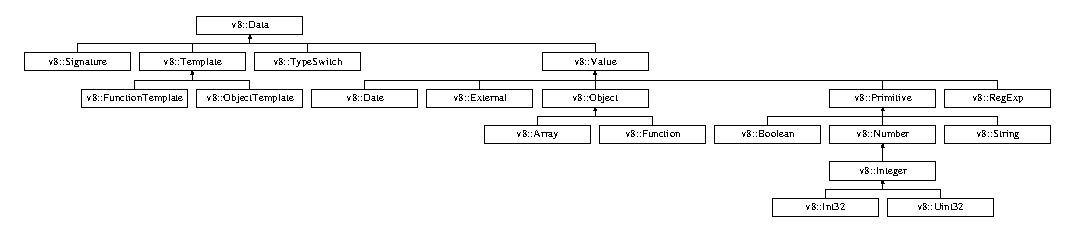
\includegraphics[height=5.159705cm]{classv8_1_1_data}
\end{center}
\end{figure}


\subsection{Detailed Description}
The superclass of values and A\+P\+I object templates. 

The documentation for this class was generated from the following file\+:\begin{DoxyCompactItemize}
\item 
deps/v8/include/v8.\+h\end{DoxyCompactItemize}

\hypertarget{classv8_1_1_date}{}\section{v8\+:\+:Date Class Reference}
\label{classv8_1_1_date}\index{v8\+::\+Date@{v8\+::\+Date}}


{\ttfamily \#include $<$v8.\+h$>$}

Inheritance diagram for v8\+:\+:Date\+:\begin{figure}[H]
\begin{center}
\leavevmode
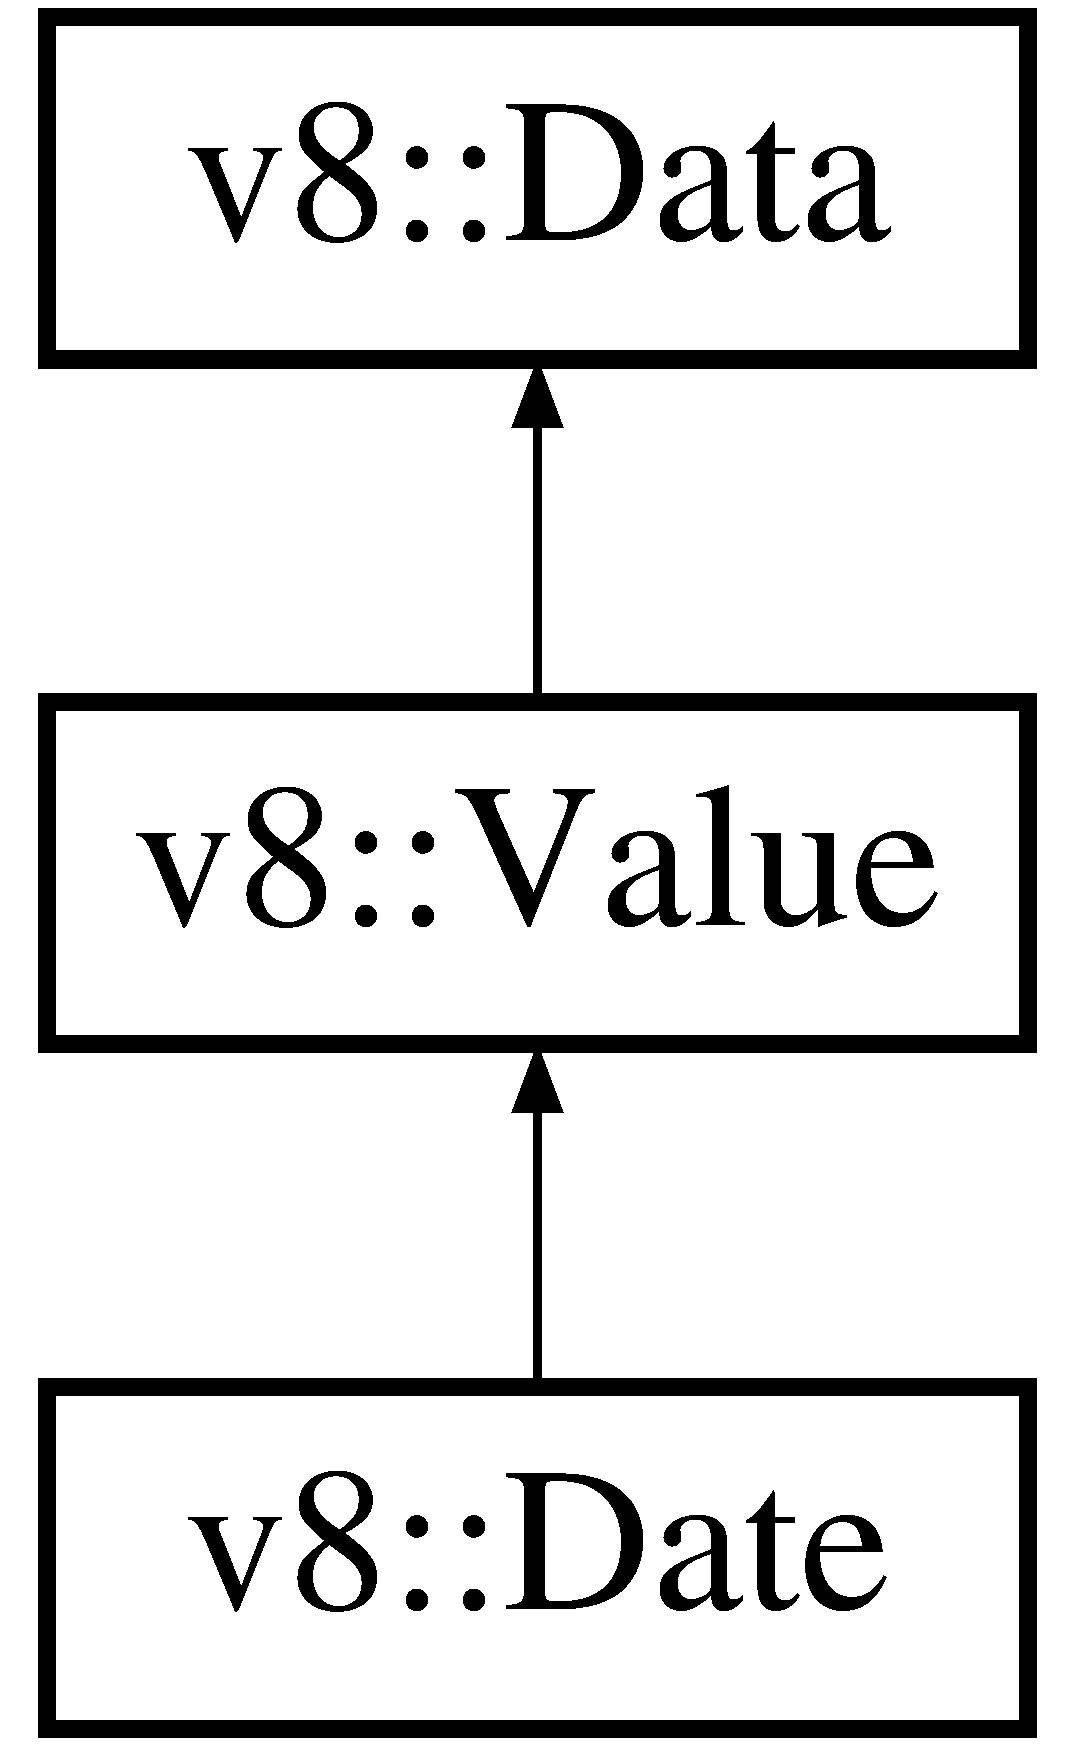
\includegraphics[height=4.000000cm]{classv8_1_1_date}
\end{center}
\end{figure}
\subsection*{Public Member Functions}
\begin{DoxyCompactItemize}
\item 
V8\+E\+X\+P\+O\+R\+T double \hyperlink{classv8_1_1_date_ae9ccdc971d9738631ed2f28ef42d8a8c}{Number\+Value} () const 
\end{DoxyCompactItemize}
\subsection*{Static Public Member Functions}
\begin{DoxyCompactItemize}
\item 
\hypertarget{classv8_1_1_date_a00a33c616710d92dae77440182cc30b2}{}static V8\+E\+X\+P\+O\+R\+T \hyperlink{classv8_1_1_local}{Local}$<$ \hyperlink{classv8_1_1_value}{Value} $>$ {\bfseries New} (double time)\label{classv8_1_1_date_a00a33c616710d92dae77440182cc30b2}

\item 
\hypertarget{classv8_1_1_date_a8e5ea7c1f28924b82922270d6596b4d3}{}static \hyperlink{classv8_1_1_date}{Date} $\ast$ {\bfseries Cast} (\hyperlink{classv8_1_1_value}{v8\+::\+Value} $\ast$obj)\label{classv8_1_1_date_a8e5ea7c1f28924b82922270d6596b4d3}

\item 
static V8\+E\+X\+P\+O\+R\+T void \hyperlink{classv8_1_1_date_ab39a9ab67254d54956d4687f3dee6816}{Date\+Time\+Configuration\+Change\+Notification} ()
\end{DoxyCompactItemize}


\subsection{Detailed Description}
An instance of the built-\/in \hyperlink{classv8_1_1_date}{Date} constructor (E\+C\+M\+A-\/262, 15.\+9). 

\subsection{Member Function Documentation}
\hypertarget{classv8_1_1_date_ab39a9ab67254d54956d4687f3dee6816}{}\index{v8\+::\+Date@{v8\+::\+Date}!Date\+Time\+Configuration\+Change\+Notification@{Date\+Time\+Configuration\+Change\+Notification}}
\index{Date\+Time\+Configuration\+Change\+Notification@{Date\+Time\+Configuration\+Change\+Notification}!v8\+::\+Date@{v8\+::\+Date}}
\subsubsection[{Date\+Time\+Configuration\+Change\+Notification}]{\setlength{\rightskip}{0pt plus 5cm}static V8\+E\+X\+P\+O\+R\+T void v8\+::\+Date\+::\+Date\+Time\+Configuration\+Change\+Notification (
\begin{DoxyParamCaption}
{}
\end{DoxyParamCaption}
)\hspace{0.3cm}{\ttfamily [static]}}\label{classv8_1_1_date_ab39a9ab67254d54956d4687f3dee6816}
Notification that the embedder has changed the time zone, daylight savings time, or other date / time configuration parameters. \hyperlink{classv8_1_1_v8}{V8} keeps a cache of various values used for date / time computation. This notification will reset those cached values for the current context so that date / time configuration changes would be reflected in the \hyperlink{classv8_1_1_date}{Date} object.

This A\+P\+I should not be called more than needed as it will negatively impact the performance of date operations. \hypertarget{classv8_1_1_date_ae9ccdc971d9738631ed2f28ef42d8a8c}{}\index{v8\+::\+Date@{v8\+::\+Date}!Number\+Value@{Number\+Value}}
\index{Number\+Value@{Number\+Value}!v8\+::\+Date@{v8\+::\+Date}}
\subsubsection[{Number\+Value}]{\setlength{\rightskip}{0pt plus 5cm}V8\+E\+X\+P\+O\+R\+T double v8\+::\+Date\+::\+Number\+Value (
\begin{DoxyParamCaption}
{}
\end{DoxyParamCaption}
) const}\label{classv8_1_1_date_ae9ccdc971d9738631ed2f28ef42d8a8c}
A specialization of Value\+::\+Number\+Value that is more efficient because we know the structure of this object. 

The documentation for this class was generated from the following file\+:\begin{DoxyCompactItemize}
\item 
deps/v8/include/v8.\+h\end{DoxyCompactItemize}

\hypertarget{classv8_1_1_debug}{}\section{v8\+:\+:Debug Class Reference}
\label{classv8_1_1_debug}\index{v8\+::\+Debug@{v8\+::\+Debug}}
\subsection*{Classes}
\begin{DoxyCompactItemize}
\item 
class \hyperlink{classv8_1_1_debug_1_1_client_data}{Client\+Data}
\item 
class \hyperlink{classv8_1_1_debug_1_1_event_details}{Event\+Details}
\item 
class \hyperlink{classv8_1_1_debug_1_1_message}{Message}
\end{DoxyCompactItemize}
\subsection*{Public Types}
\begin{DoxyCompactItemize}
\item 
typedef void($\ast$ \hyperlink{classv8_1_1_debug_a4be52510b70764b730dd1289bd9bbe37}{Event\+Callback}) (Debug\+Event event, \hyperlink{classv8_1_1_handle}{Handle}$<$ \hyperlink{classv8_1_1_object}{Object} $>$ exec\+\_\+state, \hyperlink{classv8_1_1_handle}{Handle}$<$ \hyperlink{classv8_1_1_object}{Object} $>$ event\+\_\+data, \hyperlink{classv8_1_1_handle}{Handle}$<$ \hyperlink{classv8_1_1_value}{Value} $>$ data)
\item 
typedef void($\ast$ \hyperlink{classv8_1_1_debug_aae787219311eeedcbbe2c63cf36d1e53}{Event\+Callback2}) (const \hyperlink{classv8_1_1_debug_1_1_event_details}{Event\+Details} \&event\+\_\+details)
\item 
typedef void($\ast$ \hyperlink{classv8_1_1_debug_aea5c8ab838a3b3c263a71828fb0767ac}{Message\+Handler}) (const uint16\+\_\+t $\ast$message, int length, \hyperlink{classv8_1_1_debug_1_1_client_data}{Client\+Data} $\ast$client\+\_\+data)
\item 
typedef void($\ast$ \hyperlink{classv8_1_1_debug_a0fb8f7e1f8fa47cb23f7ad72cd533c77}{Message\+Handler2}) (const \hyperlink{classv8_1_1_debug_1_1_message}{Message} \&message)
\item 
typedef void($\ast$ \hyperlink{classv8_1_1_debug_a442f686afe7d80928b57b3ff8ac3f6e7}{Host\+Dispatch\+Handler}) ()
\item 
typedef void($\ast$ \hyperlink{classv8_1_1_debug_a91cd8aa9743e3478bc63fe73abcd557c}{Debug\+Message\+Dispatch\+Handler}) ()
\end{DoxyCompactItemize}
\subsection*{Static Public Member Functions}
\begin{DoxyCompactItemize}
\item 
\hypertarget{classv8_1_1_debug_a745bc83ba29626b64151a1a3e9759e8a}{}static bool {\bfseries Set\+Debug\+Event\+Listener} (\hyperlink{classv8_1_1_debug_a4be52510b70764b730dd1289bd9bbe37}{Event\+Callback} that, \hyperlink{classv8_1_1_handle}{Handle}$<$ \hyperlink{classv8_1_1_value}{Value} $>$ data=\hyperlink{classv8_1_1_handle}{Handle}$<$ \hyperlink{classv8_1_1_value}{Value} $>$())\label{classv8_1_1_debug_a745bc83ba29626b64151a1a3e9759e8a}

\item 
\hypertarget{classv8_1_1_debug_aff46ffb7c2a8e9c6549a7ef74452fce5}{}static bool {\bfseries Set\+Debug\+Event\+Listener2} (\hyperlink{classv8_1_1_debug_aae787219311eeedcbbe2c63cf36d1e53}{Event\+Callback2} that, \hyperlink{classv8_1_1_handle}{Handle}$<$ \hyperlink{classv8_1_1_value}{Value} $>$ data=\hyperlink{classv8_1_1_handle}{Handle}$<$ \hyperlink{classv8_1_1_value}{Value} $>$())\label{classv8_1_1_debug_aff46ffb7c2a8e9c6549a7ef74452fce5}

\item 
\hypertarget{classv8_1_1_debug_a9195f4cb819848a07dc71a5bae43274d}{}static bool {\bfseries Set\+Debug\+Event\+Listener} (\hyperlink{classv8_1_1_handle}{v8\+::\+Handle}$<$ \hyperlink{classv8_1_1_object}{v8\+::\+Object} $>$ that, \hyperlink{classv8_1_1_handle}{Handle}$<$ \hyperlink{classv8_1_1_value}{Value} $>$ data=\hyperlink{classv8_1_1_handle}{Handle}$<$ \hyperlink{classv8_1_1_value}{Value} $>$())\label{classv8_1_1_debug_a9195f4cb819848a07dc71a5bae43274d}

\item 
\hypertarget{classv8_1_1_debug_a4bbac4c6f09faebe196d9403173d1707}{}static void {\bfseries Debug\+Break} (\hyperlink{classv8_1_1_isolate}{Isolate} $\ast$isolate=N\+U\+L\+L)\label{classv8_1_1_debug_a4bbac4c6f09faebe196d9403173d1707}

\item 
\hypertarget{classv8_1_1_debug_ae3177873bb9de871eaa9e7881c8a8e49}{}static void {\bfseries Cancel\+Debug\+Break} (\hyperlink{classv8_1_1_isolate}{Isolate} $\ast$isolate=N\+U\+L\+L)\label{classv8_1_1_debug_ae3177873bb9de871eaa9e7881c8a8e49}

\item 
\hypertarget{classv8_1_1_debug_ab7dba882551c995c484224c7dfebc9bd}{}static void {\bfseries Debug\+Break\+For\+Command} (\hyperlink{classv8_1_1_debug_1_1_client_data}{Client\+Data} $\ast$data=N\+U\+L\+L, \hyperlink{classv8_1_1_isolate}{Isolate} $\ast$isolate=N\+U\+L\+L)\label{classv8_1_1_debug_ab7dba882551c995c484224c7dfebc9bd}

\item 
\hypertarget{classv8_1_1_debug_ab079dd46bc3989eb990c7ef40604c5a2}{}static void {\bfseries Set\+Message\+Handler} (\hyperlink{classv8_1_1_debug_aea5c8ab838a3b3c263a71828fb0767ac}{Message\+Handler} handler, bool message\+\_\+handler\+\_\+thread=false)\label{classv8_1_1_debug_ab079dd46bc3989eb990c7ef40604c5a2}

\item 
\hypertarget{classv8_1_1_debug_a0375563b2a1e0b4ea5f70a742209bb3f}{}static void {\bfseries Set\+Message\+Handler2} (\hyperlink{classv8_1_1_debug_a0fb8f7e1f8fa47cb23f7ad72cd533c77}{Message\+Handler2} handler)\label{classv8_1_1_debug_a0375563b2a1e0b4ea5f70a742209bb3f}

\item 
\hypertarget{classv8_1_1_debug_a3fe024335cf785f8df1f072a9aea3555}{}static void {\bfseries Send\+Command} (const uint16\+\_\+t $\ast$command, int length, \hyperlink{classv8_1_1_debug_1_1_client_data}{Client\+Data} $\ast$client\+\_\+data=N\+U\+L\+L, \hyperlink{classv8_1_1_isolate}{Isolate} $\ast$isolate=N\+U\+L\+L)\label{classv8_1_1_debug_a3fe024335cf785f8df1f072a9aea3555}

\item 
\hypertarget{classv8_1_1_debug_aa55c29d5cc7b04c4fc24cd89c77f3f54}{}static void {\bfseries Set\+Host\+Dispatch\+Handler} (\hyperlink{classv8_1_1_debug_a442f686afe7d80928b57b3ff8ac3f6e7}{Host\+Dispatch\+Handler} handler, int period=100)\label{classv8_1_1_debug_aa55c29d5cc7b04c4fc24cd89c77f3f54}

\item 
static void \hyperlink{classv8_1_1_debug_a5147f6cfeb9b87a67630b8c959996e9c}{Set\+Debug\+Message\+Dispatch\+Handler} (\hyperlink{classv8_1_1_debug_a91cd8aa9743e3478bc63fe73abcd557c}{Debug\+Message\+Dispatch\+Handler} handler, bool provide\+\_\+locker=false)
\item 
static \hyperlink{classv8_1_1_local}{Local}$<$ \hyperlink{classv8_1_1_value}{Value} $>$ \hyperlink{classv8_1_1_debug_a49a3e0cf585cfd201d8ab1bc395d0593}{Call} (\hyperlink{classv8_1_1_handle}{v8\+::\+Handle}$<$ \hyperlink{classv8_1_1_function}{v8\+::\+Function} $>$ fun, \hyperlink{classv8_1_1_handle}{Handle}$<$ \hyperlink{classv8_1_1_value}{Value} $>$ data=\hyperlink{classv8_1_1_handle}{Handle}$<$ \hyperlink{classv8_1_1_value}{Value} $>$())
\item 
static \hyperlink{classv8_1_1_local}{Local}$<$ \hyperlink{classv8_1_1_value}{Value} $>$ \hyperlink{classv8_1_1_debug_aa7d07c7d5c9ee2eaaa9af310bcbf58f5}{Get\+Mirror} (\hyperlink{classv8_1_1_handle}{v8\+::\+Handle}$<$ \hyperlink{classv8_1_1_value}{v8\+::\+Value} $>$ obj)
\item 
static bool \hyperlink{classv8_1_1_debug_a78506e80b599010624c5fcde72a643a7}{Enable\+Agent} (const char $\ast$name, int port, bool wait\+\_\+for\+\_\+connection=false)
\item 
static void \hyperlink{classv8_1_1_debug_aa9b8f5fe4545f52f5937d61e972dcbf0}{Disable\+Agent} ()
\item 
static void \hyperlink{classv8_1_1_debug_a888e06766caee0380c6aa010b00e1a54}{Process\+Debug\+Messages} ()
\item 
static \hyperlink{classv8_1_1_local}{Local}$<$ \hyperlink{classv8_1_1_context}{Context} $>$ \hyperlink{classv8_1_1_debug_a2343a321b0db41324b7e8a7402f57cf0}{Get\+Debug\+Context} ()
\end{DoxyCompactItemize}


\subsection{Member Typedef Documentation}
\hypertarget{classv8_1_1_debug_a91cd8aa9743e3478bc63fe73abcd557c}{}\index{v8\+::\+Debug@{v8\+::\+Debug}!Debug\+Message\+Dispatch\+Handler@{Debug\+Message\+Dispatch\+Handler}}
\index{Debug\+Message\+Dispatch\+Handler@{Debug\+Message\+Dispatch\+Handler}!v8\+::\+Debug@{v8\+::\+Debug}}
\subsubsection[{Debug\+Message\+Dispatch\+Handler}]{\setlength{\rightskip}{0pt plus 5cm}typedef void($\ast$ v8\+::\+Debug\+::\+Debug\+Message\+Dispatch\+Handler) ()}\label{classv8_1_1_debug_a91cd8aa9743e3478bc63fe73abcd557c}
Callback function for the host to ensure debug messages are processed. \hypertarget{classv8_1_1_debug_a4be52510b70764b730dd1289bd9bbe37}{}\index{v8\+::\+Debug@{v8\+::\+Debug}!Event\+Callback@{Event\+Callback}}
\index{Event\+Callback@{Event\+Callback}!v8\+::\+Debug@{v8\+::\+Debug}}
\subsubsection[{Event\+Callback}]{\setlength{\rightskip}{0pt plus 5cm}typedef void($\ast$ v8\+::\+Debug\+::\+Event\+Callback) (Debug\+Event event, {\bf Handle}$<$ {\bf Object} $>$ exec\+\_\+state, {\bf Handle}$<$ {\bf Object} $>$ event\+\_\+data, {\bf Handle}$<$ {\bf Value} $>$ data)}\label{classv8_1_1_debug_a4be52510b70764b730dd1289bd9bbe37}
\hyperlink{classv8_1_1_debug}{Debug} event callback function.


\begin{DoxyParams}{Parameters}
{\em event} & the type of the debug event that triggered the callback (enum Debug\+Event) \\
\hline
{\em exec\+\_\+state} & execution state (Java\+Script object) \\
\hline
{\em event\+\_\+data} & event specific data (Java\+Script object) \\
\hline
{\em data} & value passed by the user to Set\+Debug\+Event\+Listener \\
\hline
\end{DoxyParams}
\hypertarget{classv8_1_1_debug_aae787219311eeedcbbe2c63cf36d1e53}{}\index{v8\+::\+Debug@{v8\+::\+Debug}!Event\+Callback2@{Event\+Callback2}}
\index{Event\+Callback2@{Event\+Callback2}!v8\+::\+Debug@{v8\+::\+Debug}}
\subsubsection[{Event\+Callback2}]{\setlength{\rightskip}{0pt plus 5cm}typedef void($\ast$ v8\+::\+Debug\+::\+Event\+Callback2) (const {\bf Event\+Details} \&event\+\_\+details)}\label{classv8_1_1_debug_aae787219311eeedcbbe2c63cf36d1e53}
\hyperlink{classv8_1_1_debug}{Debug} event callback function.


\begin{DoxyParams}{Parameters}
{\em event\+\_\+details} & object providing information about the debug event\\
\hline
\end{DoxyParams}
A Event\+Callback2 does not take possession of the event data, and must not rely on the data persisting after the handler returns. \hypertarget{classv8_1_1_debug_a442f686afe7d80928b57b3ff8ac3f6e7}{}\index{v8\+::\+Debug@{v8\+::\+Debug}!Host\+Dispatch\+Handler@{Host\+Dispatch\+Handler}}
\index{Host\+Dispatch\+Handler@{Host\+Dispatch\+Handler}!v8\+::\+Debug@{v8\+::\+Debug}}
\subsubsection[{Host\+Dispatch\+Handler}]{\setlength{\rightskip}{0pt plus 5cm}typedef void($\ast$ v8\+::\+Debug\+::\+Host\+Dispatch\+Handler) ()}\label{classv8_1_1_debug_a442f686afe7d80928b57b3ff8ac3f6e7}
\hyperlink{classv8_1_1_debug}{Debug} host dispatch callback function. \hypertarget{classv8_1_1_debug_aea5c8ab838a3b3c263a71828fb0767ac}{}\index{v8\+::\+Debug@{v8\+::\+Debug}!Message\+Handler@{Message\+Handler}}
\index{Message\+Handler@{Message\+Handler}!v8\+::\+Debug@{v8\+::\+Debug}}
\subsubsection[{Message\+Handler}]{\setlength{\rightskip}{0pt plus 5cm}typedef void($\ast$ v8\+::\+Debug\+::\+Message\+Handler) (const uint16\+\_\+t $\ast$message, int length, {\bf Client\+Data} $\ast$client\+\_\+data)}\label{classv8_1_1_debug_aea5c8ab838a3b3c263a71828fb0767ac}
\hyperlink{classv8_1_1_debug}{Debug} message callback function.


\begin{DoxyParams}{Parameters}
{\em message} & the debug message handler message object \\
\hline
{\em length} & length of the message \\
\hline
{\em client\+\_\+data} & the data value passed when registering the message handler\\
\hline
\end{DoxyParams}
A Message\+Handler does not take possession of the message string, and must not rely on the data persisting after the handler returns.

This message handler is deprecated. Use Message\+Handler2 instead. \hypertarget{classv8_1_1_debug_a0fb8f7e1f8fa47cb23f7ad72cd533c77}{}\index{v8\+::\+Debug@{v8\+::\+Debug}!Message\+Handler2@{Message\+Handler2}}
\index{Message\+Handler2@{Message\+Handler2}!v8\+::\+Debug@{v8\+::\+Debug}}
\subsubsection[{Message\+Handler2}]{\setlength{\rightskip}{0pt plus 5cm}typedef void($\ast$ v8\+::\+Debug\+::\+Message\+Handler2) (const {\bf Message} \&message)}\label{classv8_1_1_debug_a0fb8f7e1f8fa47cb23f7ad72cd533c77}
\hyperlink{classv8_1_1_debug}{Debug} message callback function.


\begin{DoxyParams}{Parameters}
{\em message} & the debug message handler message object\\
\hline
\end{DoxyParams}
A Message\+Handler does not take possession of the message data, and must not rely on the data persisting after the handler returns. 

\subsection{Member Function Documentation}
\hypertarget{classv8_1_1_debug_a49a3e0cf585cfd201d8ab1bc395d0593}{}\index{v8\+::\+Debug@{v8\+::\+Debug}!Call@{Call}}
\index{Call@{Call}!v8\+::\+Debug@{v8\+::\+Debug}}
\subsubsection[{Call}]{\setlength{\rightskip}{0pt plus 5cm}static {\bf Local}$<${\bf Value}$>$ v8\+::\+Debug\+::\+Call (
\begin{DoxyParamCaption}
\item[{{\bf v8\+::\+Handle}$<$ {\bf v8\+::\+Function} $>$}]{fun, }
\item[{{\bf Handle}$<$ {\bf Value} $>$}]{data = {\ttfamily {\bf Handle}$<$~{\bf Value}~$>$()}}
\end{DoxyParamCaption}
)\hspace{0.3cm}{\ttfamily [static]}}\label{classv8_1_1_debug_a49a3e0cf585cfd201d8ab1bc395d0593}
Run a Java\+Script function in the debugger. 
\begin{DoxyParams}{Parameters}
{\em fun} & the function to call \\
\hline
{\em data} & passed as second argument to the function With this call the debugger is entered and the function specified is called with the execution state as the first argument. This makes it possible to get access to information otherwise not available during normal Java\+Script execution e.\+g. details on stack frames. Receiver of the function call will be the debugger context global object, however this is a subject to change. The following example shows a Java\+Script function which when passed to \hyperlink{classv8_1_1_debug_a49a3e0cf585cfd201d8ab1bc395d0593}{v8\+::\+Debug\+::\+Call} will return the current line of Java\+Script execution.\\
\hline
\end{DoxyParams}

\begin{DoxyCode}
\textcolor{keyword}{function} frame\_source\_line(exec\_state) \{
  \textcolor{keywordflow}{return} exec\_state.frame(0).sourceLine();
\}
\end{DoxyCode}
 \hypertarget{classv8_1_1_debug_aa9b8f5fe4545f52f5937d61e972dcbf0}{}\index{v8\+::\+Debug@{v8\+::\+Debug}!Disable\+Agent@{Disable\+Agent}}
\index{Disable\+Agent@{Disable\+Agent}!v8\+::\+Debug@{v8\+::\+Debug}}
\subsubsection[{Disable\+Agent}]{\setlength{\rightskip}{0pt plus 5cm}static void v8\+::\+Debug\+::\+Disable\+Agent (
\begin{DoxyParamCaption}
{}
\end{DoxyParamCaption}
)\hspace{0.3cm}{\ttfamily [static]}}\label{classv8_1_1_debug_aa9b8f5fe4545f52f5937d61e972dcbf0}
Disable the \hyperlink{classv8_1_1_v8}{V8} builtin debug agent. The T\+C\+P/\+I\+P connection will be closed. \hypertarget{classv8_1_1_debug_a78506e80b599010624c5fcde72a643a7}{}\index{v8\+::\+Debug@{v8\+::\+Debug}!Enable\+Agent@{Enable\+Agent}}
\index{Enable\+Agent@{Enable\+Agent}!v8\+::\+Debug@{v8\+::\+Debug}}
\subsubsection[{Enable\+Agent}]{\setlength{\rightskip}{0pt plus 5cm}static bool v8\+::\+Debug\+::\+Enable\+Agent (
\begin{DoxyParamCaption}
\item[{const char $\ast$}]{name, }
\item[{int}]{port, }
\item[{bool}]{wait\+\_\+for\+\_\+connection = {\ttfamily false}}
\end{DoxyParamCaption}
)\hspace{0.3cm}{\ttfamily [static]}}\label{classv8_1_1_debug_a78506e80b599010624c5fcde72a643a7}
Enable the \hyperlink{classv8_1_1_v8}{V8} builtin debug agent. The debugger agent will listen on the supplied T\+C\+P/\+I\+P port for remote debugger connection. 
\begin{DoxyParams}{Parameters}
{\em name} & the name of the embedding application \\
\hline
{\em port} & the T\+C\+P/\+I\+P port to listen on \\
\hline
{\em wait\+\_\+for\+\_\+connection} & whether \hyperlink{classv8_1_1_v8}{V8} should pause on a first statement allowing remote debugger to connect before anything interesting happened \\
\hline
\end{DoxyParams}
\hypertarget{classv8_1_1_debug_a2343a321b0db41324b7e8a7402f57cf0}{}\index{v8\+::\+Debug@{v8\+::\+Debug}!Get\+Debug\+Context@{Get\+Debug\+Context}}
\index{Get\+Debug\+Context@{Get\+Debug\+Context}!v8\+::\+Debug@{v8\+::\+Debug}}
\subsubsection[{Get\+Debug\+Context}]{\setlength{\rightskip}{0pt plus 5cm}static {\bf Local}$<${\bf Context}$>$ v8\+::\+Debug\+::\+Get\+Debug\+Context (
\begin{DoxyParamCaption}
{}
\end{DoxyParamCaption}
)\hspace{0.3cm}{\ttfamily [static]}}\label{classv8_1_1_debug_a2343a321b0db41324b7e8a7402f57cf0}
Debugger is running in its own context which is entered while debugger messages are being dispatched. This is an explicit getter for this debugger context. Note that the content of the debugger context is subject to change. \hypertarget{classv8_1_1_debug_aa7d07c7d5c9ee2eaaa9af310bcbf58f5}{}\index{v8\+::\+Debug@{v8\+::\+Debug}!Get\+Mirror@{Get\+Mirror}}
\index{Get\+Mirror@{Get\+Mirror}!v8\+::\+Debug@{v8\+::\+Debug}}
\subsubsection[{Get\+Mirror}]{\setlength{\rightskip}{0pt plus 5cm}static {\bf Local}$<${\bf Value}$>$ v8\+::\+Debug\+::\+Get\+Mirror (
\begin{DoxyParamCaption}
\item[{{\bf v8\+::\+Handle}$<$ {\bf v8\+::\+Value} $>$}]{obj}
\end{DoxyParamCaption}
)\hspace{0.3cm}{\ttfamily [static]}}\label{classv8_1_1_debug_aa7d07c7d5c9ee2eaaa9af310bcbf58f5}
Returns a mirror object for the given object. \hypertarget{classv8_1_1_debug_a888e06766caee0380c6aa010b00e1a54}{}\index{v8\+::\+Debug@{v8\+::\+Debug}!Process\+Debug\+Messages@{Process\+Debug\+Messages}}
\index{Process\+Debug\+Messages@{Process\+Debug\+Messages}!v8\+::\+Debug@{v8\+::\+Debug}}
\subsubsection[{Process\+Debug\+Messages}]{\setlength{\rightskip}{0pt plus 5cm}static void v8\+::\+Debug\+::\+Process\+Debug\+Messages (
\begin{DoxyParamCaption}
{}
\end{DoxyParamCaption}
)\hspace{0.3cm}{\ttfamily [static]}}\label{classv8_1_1_debug_a888e06766caee0380c6aa010b00e1a54}
Makes \hyperlink{classv8_1_1_v8}{V8} process all pending debug messages.

From \hyperlink{classv8_1_1_v8}{V8} point of view all debug messages come asynchronously (e.\+g. from remote debugger) but they all must be handled synchronously\+: \hyperlink{classv8_1_1_v8}{V8} cannot do 2 things at one time so normal script execution must be interrupted for a while.

Generally when message arrives \hyperlink{classv8_1_1_v8}{V8} may be in one of 3 states\+:
\begin{DoxyEnumerate}
\item \hyperlink{classv8_1_1_v8}{V8} is running script; \hyperlink{classv8_1_1_v8}{V8} will automatically interrupt and process all pending messages (however auto\+\_\+break flag should be enabled);
\item \hyperlink{classv8_1_1_v8}{V8} is suspended on debug breakpoint; in this state \hyperlink{classv8_1_1_v8}{V8} is dedicated to reading and processing debug messages;
\item \hyperlink{classv8_1_1_v8}{V8} is not running at all or has called some long-\/working C++ function; by default it means that processing of all debug messages will be deferred until \hyperlink{classv8_1_1_v8}{V8} gets control again; however, embedding application may improve this by manually calling this method.
\end{DoxyEnumerate}

It makes sense to call this method whenever a new debug message arrived and \hyperlink{classv8_1_1_v8}{V8} is not already running. Method \hyperlink{classv8_1_1_debug_a5147f6cfeb9b87a67630b8c959996e9c}{v8\+::\+Debug\+::\+Set\+Debug\+Message\+Dispatch\+Handler} should help with the former condition.

Technically this method in many senses is equivalent to executing empty script\+:
\begin{DoxyEnumerate}
\item It does nothing except for processing all pending debug messages.
\item It should be invoked with the same precautions and from the same context as \hyperlink{classv8_1_1_v8}{V8} script would be invoked from, because\+: a. with \char`\"{}evaluate\char`\"{} command it can do whatever normal script can do, including all native calls; b. no other thread should call \hyperlink{classv8_1_1_v8}{V8} while this method is running (\hyperlink{classv8_1_1_locker}{v8\+::\+Locker} may be used here).
\end{DoxyEnumerate}

\char`\"{}\+Evaluate\char`\"{} debug command behavior currently is not specified in scope of this method. \hypertarget{classv8_1_1_debug_a5147f6cfeb9b87a67630b8c959996e9c}{}\index{v8\+::\+Debug@{v8\+::\+Debug}!Set\+Debug\+Message\+Dispatch\+Handler@{Set\+Debug\+Message\+Dispatch\+Handler}}
\index{Set\+Debug\+Message\+Dispatch\+Handler@{Set\+Debug\+Message\+Dispatch\+Handler}!v8\+::\+Debug@{v8\+::\+Debug}}
\subsubsection[{Set\+Debug\+Message\+Dispatch\+Handler}]{\setlength{\rightskip}{0pt plus 5cm}static void v8\+::\+Debug\+::\+Set\+Debug\+Message\+Dispatch\+Handler (
\begin{DoxyParamCaption}
\item[{{\bf Debug\+Message\+Dispatch\+Handler}}]{handler, }
\item[{bool}]{provide\+\_\+locker = {\ttfamily false}}
\end{DoxyParamCaption}
)\hspace{0.3cm}{\ttfamily [static]}}\label{classv8_1_1_debug_a5147f6cfeb9b87a67630b8c959996e9c}
Register a callback function to be called when a debug message has been received and is ready to be processed. For the debug messages to be processed \hyperlink{classv8_1_1_v8}{V8} needs to be entered, and in certain embedding scenarios this callback can be used to make sure \hyperlink{classv8_1_1_v8}{V8} is entered for the debug message to be processed. Note that debug messages will only be processed if there is a \hyperlink{classv8_1_1_v8}{V8} break. This can happen automatically by using the option --debugger-\/auto-\/break. 
\begin{DoxyParams}{Parameters}
{\em provide\+\_\+locker} & requires that \hyperlink{classv8_1_1_v8}{V8} acquires \hyperlink{classv8_1_1_locker}{v8\+::\+Locker} for you before calling handler \\
\hline
\end{DoxyParams}


The documentation for this class was generated from the following file\+:\begin{DoxyCompactItemize}
\item 
deps/v8/include/v8-\/debug.\+h\end{DoxyCompactItemize}

\hypertarget{classv8_1_1_declare_extension}{}\section{v8\+:\+:Declare\+Extension Class Reference}
\label{classv8_1_1_declare_extension}\index{v8\+::\+Declare\+Extension@{v8\+::\+Declare\+Extension}}


{\ttfamily \#include $<$v8.\+h$>$}

\subsection*{Public Member Functions}
\begin{DoxyCompactItemize}
\item 
\hypertarget{classv8_1_1_declare_extension_af3b52757ae0cf848e1cdc007c485d04d}{}V8\+\_\+\+I\+N\+L\+I\+N\+E {\bfseries Declare\+Extension} (\hyperlink{classv8_1_1_extension}{Extension} $\ast$extension)\label{classv8_1_1_declare_extension_af3b52757ae0cf848e1cdc007c485d04d}

\end{DoxyCompactItemize}


\subsection{Detailed Description}
Ignore 

The documentation for this class was generated from the following file\+:\begin{DoxyCompactItemize}
\item 
deps/v8/include/v8.\+h\end{DoxyCompactItemize}

\hypertarget{classv8_1_1_debug_1_1_event_details}{}\section{v8\+:\+:Debug\+:\+:Event\+Details Class Reference}
\label{classv8_1_1_debug_1_1_event_details}\index{v8\+::\+Debug\+::\+Event\+Details@{v8\+::\+Debug\+::\+Event\+Details}}


{\ttfamily \#include $<$v8-\/debug.\+h$>$}

\subsection*{Public Member Functions}
\begin{DoxyCompactItemize}
\item 
virtual Debug\+Event \hyperlink{classv8_1_1_debug_1_1_event_details_ac871568e8cfd43bbf2cdac62add34ed0}{Get\+Event} () const =0
\item 
virtual \hyperlink{classv8_1_1_local}{Handle}$<$ \hyperlink{classv8_1_1_object}{Object} $>$ \hyperlink{classv8_1_1_debug_1_1_event_details_abf0997988e1e3f0780c0d3f19b4e3b8a}{Get\+Execution\+State} () const =0
\item 
\hypertarget{classv8_1_1_debug_1_1_event_details_af8003f761cd535a07be5448a43d94c9f}{}virtual \hyperlink{classv8_1_1_local}{Handle}$<$ \hyperlink{classv8_1_1_object}{Object} $>$ {\bfseries Get\+Event\+Data} () const =0\label{classv8_1_1_debug_1_1_event_details_af8003f761cd535a07be5448a43d94c9f}

\item 
virtual \hyperlink{classv8_1_1_local}{Handle}$<$ \hyperlink{classv8_1_1_context}{Context} $>$ \hyperlink{classv8_1_1_debug_1_1_event_details_a2c98fc8b2848105c37fc60a04b35dfa5}{Get\+Event\+Context} () const =0
\item 
virtual \hyperlink{classv8_1_1_local}{Handle}$<$ \hyperlink{classv8_1_1_value}{Value} $>$ \hyperlink{classv8_1_1_debug_1_1_event_details_a3c1eff8397db7c91e9c687f48d400665}{Get\+Callback\+Data} () const =0
\item 
virtual \hyperlink{classv8_1_1_debug_1_1_client_data}{Client\+Data} $\ast$ \hyperlink{classv8_1_1_debug_1_1_event_details_ae663e7607d27c3252049eea077a83e08}{Get\+Client\+Data} () const =0
\end{DoxyCompactItemize}


\subsection{Detailed Description}
An event details object passed to the debug event listener. 

\subsection{Member Function Documentation}
\hypertarget{classv8_1_1_debug_1_1_event_details_a3c1eff8397db7c91e9c687f48d400665}{}\index{v8\+::\+Debug\+::\+Event\+Details@{v8\+::\+Debug\+::\+Event\+Details}!Get\+Callback\+Data@{Get\+Callback\+Data}}
\index{Get\+Callback\+Data@{Get\+Callback\+Data}!v8\+::\+Debug\+::\+Event\+Details@{v8\+::\+Debug\+::\+Event\+Details}}
\subsubsection[{Get\+Callback\+Data}]{\setlength{\rightskip}{0pt plus 5cm}virtual {\bf Handle}$<${\bf Value}$>$ v8\+::\+Debug\+::\+Event\+Details\+::\+Get\+Callback\+Data (
\begin{DoxyParamCaption}
{}
\end{DoxyParamCaption}
) const\hspace{0.3cm}{\ttfamily [pure virtual]}}\label{classv8_1_1_debug_1_1_event_details_a3c1eff8397db7c91e9c687f48d400665}
Client data passed with the corresponding callback when it was registered. \hypertarget{classv8_1_1_debug_1_1_event_details_ae663e7607d27c3252049eea077a83e08}{}\index{v8\+::\+Debug\+::\+Event\+Details@{v8\+::\+Debug\+::\+Event\+Details}!Get\+Client\+Data@{Get\+Client\+Data}}
\index{Get\+Client\+Data@{Get\+Client\+Data}!v8\+::\+Debug\+::\+Event\+Details@{v8\+::\+Debug\+::\+Event\+Details}}
\subsubsection[{Get\+Client\+Data}]{\setlength{\rightskip}{0pt plus 5cm}virtual {\bf Client\+Data}$\ast$ v8\+::\+Debug\+::\+Event\+Details\+::\+Get\+Client\+Data (
\begin{DoxyParamCaption}
{}
\end{DoxyParamCaption}
) const\hspace{0.3cm}{\ttfamily [pure virtual]}}\label{classv8_1_1_debug_1_1_event_details_ae663e7607d27c3252049eea077a83e08}
Client data passed to Debug\+Break\+For\+Command function. The debugger takes ownership of the data and will delete it even if there is no message handler. \hypertarget{classv8_1_1_debug_1_1_event_details_ac871568e8cfd43bbf2cdac62add34ed0}{}\index{v8\+::\+Debug\+::\+Event\+Details@{v8\+::\+Debug\+::\+Event\+Details}!Get\+Event@{Get\+Event}}
\index{Get\+Event@{Get\+Event}!v8\+::\+Debug\+::\+Event\+Details@{v8\+::\+Debug\+::\+Event\+Details}}
\subsubsection[{Get\+Event}]{\setlength{\rightskip}{0pt plus 5cm}virtual Debug\+Event v8\+::\+Debug\+::\+Event\+Details\+::\+Get\+Event (
\begin{DoxyParamCaption}
{}
\end{DoxyParamCaption}
) const\hspace{0.3cm}{\ttfamily [pure virtual]}}\label{classv8_1_1_debug_1_1_event_details_ac871568e8cfd43bbf2cdac62add34ed0}
Event type. \hypertarget{classv8_1_1_debug_1_1_event_details_a2c98fc8b2848105c37fc60a04b35dfa5}{}\index{v8\+::\+Debug\+::\+Event\+Details@{v8\+::\+Debug\+::\+Event\+Details}!Get\+Event\+Context@{Get\+Event\+Context}}
\index{Get\+Event\+Context@{Get\+Event\+Context}!v8\+::\+Debug\+::\+Event\+Details@{v8\+::\+Debug\+::\+Event\+Details}}
\subsubsection[{Get\+Event\+Context}]{\setlength{\rightskip}{0pt plus 5cm}virtual {\bf Handle}$<${\bf Context}$>$ v8\+::\+Debug\+::\+Event\+Details\+::\+Get\+Event\+Context (
\begin{DoxyParamCaption}
{}
\end{DoxyParamCaption}
) const\hspace{0.3cm}{\ttfamily [pure virtual]}}\label{classv8_1_1_debug_1_1_event_details_a2c98fc8b2848105c37fc60a04b35dfa5}
Get the context active when the debug event happened. Note this is not the current active context as the Java\+Script part of the debugger is running in its own context which is entered at this point. \hypertarget{classv8_1_1_debug_1_1_event_details_abf0997988e1e3f0780c0d3f19b4e3b8a}{}\index{v8\+::\+Debug\+::\+Event\+Details@{v8\+::\+Debug\+::\+Event\+Details}!Get\+Execution\+State@{Get\+Execution\+State}}
\index{Get\+Execution\+State@{Get\+Execution\+State}!v8\+::\+Debug\+::\+Event\+Details@{v8\+::\+Debug\+::\+Event\+Details}}
\subsubsection[{Get\+Execution\+State}]{\setlength{\rightskip}{0pt plus 5cm}virtual {\bf Handle}$<${\bf Object}$>$ v8\+::\+Debug\+::\+Event\+Details\+::\+Get\+Execution\+State (
\begin{DoxyParamCaption}
{}
\end{DoxyParamCaption}
) const\hspace{0.3cm}{\ttfamily [pure virtual]}}\label{classv8_1_1_debug_1_1_event_details_abf0997988e1e3f0780c0d3f19b4e3b8a}
Access to execution state and event data of the debug event. Don\textquotesingle{}t store these cross callbacks as their content becomes invalid. 

The documentation for this class was generated from the following file\+:\begin{DoxyCompactItemize}
\item 
deps/v8/include/v8-\/debug.\+h\end{DoxyCompactItemize}

\hypertarget{classv8_1_1_exception}{}\section{v8\+:\+:Exception Class Reference}
\label{classv8_1_1_exception}\index{v8\+::\+Exception@{v8\+::\+Exception}}


{\ttfamily \#include $<$v8.\+h$>$}

\subsection*{Static Public Member Functions}
\begin{DoxyCompactItemize}
\item 
\hypertarget{classv8_1_1_exception_a3ce2406b4aa50f8639450ec11baee26f}{}static \hyperlink{classv8_1_1_local}{Local}$<$ \hyperlink{classv8_1_1_value}{Value} $>$ {\bfseries Range\+Error} (\hyperlink{classv8_1_1_handle}{Handle}$<$ \hyperlink{classv8_1_1_string}{String} $>$ message)\label{classv8_1_1_exception_a3ce2406b4aa50f8639450ec11baee26f}

\item 
\hypertarget{classv8_1_1_exception_adef7d49c3370594fbc97ee68c3fcbf29}{}static \hyperlink{classv8_1_1_local}{Local}$<$ \hyperlink{classv8_1_1_value}{Value} $>$ {\bfseries Reference\+Error} (\hyperlink{classv8_1_1_handle}{Handle}$<$ \hyperlink{classv8_1_1_string}{String} $>$ message)\label{classv8_1_1_exception_adef7d49c3370594fbc97ee68c3fcbf29}

\item 
\hypertarget{classv8_1_1_exception_a938d1b571e9021121ad0f820c5e95114}{}static \hyperlink{classv8_1_1_local}{Local}$<$ \hyperlink{classv8_1_1_value}{Value} $>$ {\bfseries Syntax\+Error} (\hyperlink{classv8_1_1_handle}{Handle}$<$ \hyperlink{classv8_1_1_string}{String} $>$ message)\label{classv8_1_1_exception_a938d1b571e9021121ad0f820c5e95114}

\item 
\hypertarget{classv8_1_1_exception_a61645d9d6b46cf76f2a8eccfe7039b90}{}static \hyperlink{classv8_1_1_local}{Local}$<$ \hyperlink{classv8_1_1_value}{Value} $>$ {\bfseries Type\+Error} (\hyperlink{classv8_1_1_handle}{Handle}$<$ \hyperlink{classv8_1_1_string}{String} $>$ message)\label{classv8_1_1_exception_a61645d9d6b46cf76f2a8eccfe7039b90}

\item 
\hypertarget{classv8_1_1_exception_ae598e4b24cf37c9986b6ad1bed858aee}{}static \hyperlink{classv8_1_1_local}{Local}$<$ \hyperlink{classv8_1_1_value}{Value} $>$ {\bfseries Error} (\hyperlink{classv8_1_1_handle}{Handle}$<$ \hyperlink{classv8_1_1_string}{String} $>$ message)\label{classv8_1_1_exception_ae598e4b24cf37c9986b6ad1bed858aee}

\end{DoxyCompactItemize}


\subsection{Detailed Description}
Create new error objects by calling the corresponding error object constructor with the message. 

The documentation for this class was generated from the following file\+:\begin{DoxyCompactItemize}
\item 
deps/v8/include/v8.\+h\end{DoxyCompactItemize}

\hypertarget{classv8_1_1_extension}{}\section{v8\+:\+:Extension Class Reference}
\label{classv8_1_1_extension}\index{v8\+::\+Extension@{v8\+::\+Extension}}


{\ttfamily \#include $<$v8.\+h$>$}

\subsection*{Public Member Functions}
\begin{DoxyCompactItemize}
\item 
\hypertarget{classv8_1_1_extension_a10868673b7801cc1139ca3bc09bcfcf6}{}{\bfseries Extension} (const char $\ast$name, const char $\ast$source=0, int dep\+\_\+count=0, const char $\ast$$\ast$deps=0, int source\+\_\+length=-\/1)\label{classv8_1_1_extension_a10868673b7801cc1139ca3bc09bcfcf6}

\item 
\hypertarget{classv8_1_1_extension_acd2dc16a3afa2ec737e9bc9adea977be}{}virtual \hyperlink{classv8_1_1_handle}{v8\+::\+Handle}$<$ \hyperlink{classv8_1_1_function_template}{v8\+::\+Function\+Template} $>$ {\bfseries Get\+Native\+Function\+Template} (\hyperlink{classv8_1_1_isolate}{v8\+::\+Isolate} $\ast$isolate, \hyperlink{classv8_1_1_handle}{v8\+::\+Handle}$<$ \hyperlink{classv8_1_1_string}{v8\+::\+String} $>$ name)\label{classv8_1_1_extension_acd2dc16a3afa2ec737e9bc9adea977be}

\item 
\hypertarget{classv8_1_1_extension_a183946edbf28789f7cddecdad2d26f96}{}const char $\ast$ {\bfseries name} () const \label{classv8_1_1_extension_a183946edbf28789f7cddecdad2d26f96}

\item 
\hypertarget{classv8_1_1_extension_a91da6067f79c5c354aa3184ed0746966}{}size\+\_\+t {\bfseries source\+\_\+length} () const \label{classv8_1_1_extension_a91da6067f79c5c354aa3184ed0746966}

\item 
\hypertarget{classv8_1_1_extension_a97aa9a425f31d453161540e37c19c0ce}{}const \hyperlink{classv8_1_1_string_1_1_external_ascii_string_resource}{String\+::\+External\+Ascii\+String\+Resource} $\ast$ {\bfseries source} () const \label{classv8_1_1_extension_a97aa9a425f31d453161540e37c19c0ce}

\item 
\hypertarget{classv8_1_1_extension_a7623b08e3bc42d903bd923a00317b7f9}{}int {\bfseries dependency\+\_\+count} ()\label{classv8_1_1_extension_a7623b08e3bc42d903bd923a00317b7f9}

\item 
\hypertarget{classv8_1_1_extension_adbec8a811d5a4554678da4a5d55dda6d}{}const char $\ast$$\ast$ {\bfseries dependencies} ()\label{classv8_1_1_extension_adbec8a811d5a4554678da4a5d55dda6d}

\item 
\hypertarget{classv8_1_1_extension_af5b752ba211315b6e9dac5c0e6e638e8}{}void {\bfseries set\+\_\+auto\+\_\+enable} (bool value)\label{classv8_1_1_extension_af5b752ba211315b6e9dac5c0e6e638e8}

\item 
\hypertarget{classv8_1_1_extension_aee87ef4f9c3d7880fc3b28765d28e516}{}bool {\bfseries auto\+\_\+enable} ()\label{classv8_1_1_extension_aee87ef4f9c3d7880fc3b28765d28e516}

\end{DoxyCompactItemize}


\subsection{Detailed Description}
Ignore 

The documentation for this class was generated from the following file\+:\begin{DoxyCompactItemize}
\item 
deps/v8/include/v8.\+h\end{DoxyCompactItemize}

\hypertarget{classv8_1_1_extension_configuration}{}\section{v8\+:\+:Extension\+Configuration Class Reference}
\label{classv8_1_1_extension_configuration}\index{v8\+::\+Extension\+Configuration@{v8\+::\+Extension\+Configuration}}


{\ttfamily \#include $<$v8.\+h$>$}

\subsection*{Public Member Functions}
\begin{DoxyCompactItemize}
\item 
\hypertarget{classv8_1_1_extension_configuration_a1189e46efe963db4aa7340cc767f276a}{}{\bfseries Extension\+Configuration} (int name\+\_\+count, const char $\ast$names\mbox{[}$\,$\mbox{]})\label{classv8_1_1_extension_configuration_a1189e46efe963db4aa7340cc767f276a}

\end{DoxyCompactItemize}
\subsection*{Friends}
\begin{DoxyCompactItemize}
\item 
\hypertarget{classv8_1_1_extension_configuration_ac7b520085953e146d849e05253267f72}{}class {\bfseries Implementation\+Utilities}\label{classv8_1_1_extension_configuration_ac7b520085953e146d849e05253267f72}

\end{DoxyCompactItemize}


\subsection{Detailed Description}
Ignore 

The documentation for this class was generated from the following file\+:\begin{DoxyCompactItemize}
\item 
deps/v8/include/v8.\+h\end{DoxyCompactItemize}

\hypertarget{classv8_1_1_external}{}\section{v8\+:\+:External Class Reference}
\label{classv8_1_1_external}\index{v8\+::\+External@{v8\+::\+External}}


{\ttfamily \#include $<$v8.\+h$>$}

Inheritance diagram for v8\+:\+:External\+:\begin{figure}[H]
\begin{center}
\leavevmode
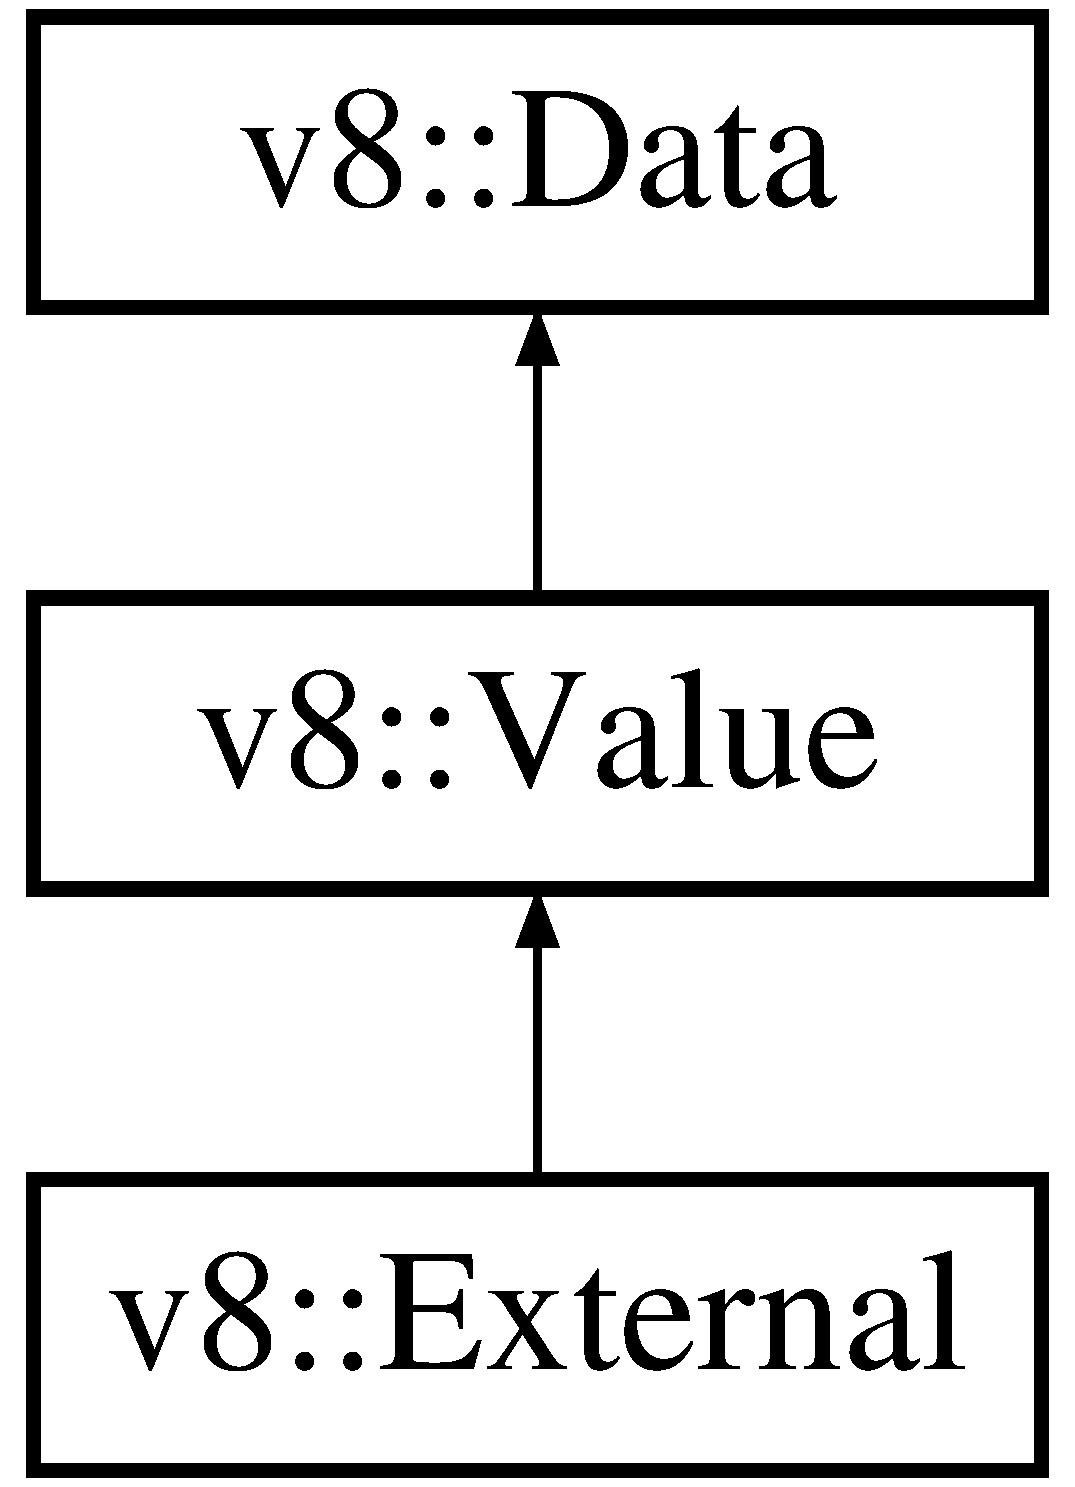
\includegraphics[height=3.000000cm]{classv8_1_1_external}
\end{center}
\end{figure}
\subsection*{Public Member Functions}
\begin{DoxyCompactItemize}
\item 
\hypertarget{classv8_1_1_external_a17d89761a1fa35f7b526c3e1305738d1}{}V8\+E\+X\+P\+O\+R\+T void $\ast$ {\bfseries Value} () const \label{classv8_1_1_external_a17d89761a1fa35f7b526c3e1305738d1}

\end{DoxyCompactItemize}
\subsection*{Static Public Member Functions}
\begin{DoxyCompactItemize}
\item 
\hypertarget{classv8_1_1_external_ae22c392d352c75ebded75092337aaedd}{}static V8\+E\+X\+P\+O\+R\+T \hyperlink{classv8_1_1_local}{Local}$<$ \hyperlink{classv8_1_1_value}{Value} $>$ {\bfseries Wrap} (void $\ast$data)\label{classv8_1_1_external_ae22c392d352c75ebded75092337aaedd}

\item 
\hypertarget{classv8_1_1_external_a8a3d966cf493d986adb7a53a17651a8b}{}static void $\ast$ {\bfseries Unwrap} (\hyperlink{classv8_1_1_handle}{Handle}$<$ \hyperlink{classv8_1_1_value}{Value} $>$ obj)\label{classv8_1_1_external_a8a3d966cf493d986adb7a53a17651a8b}

\item 
\hypertarget{classv8_1_1_external_ae4ff3030216c7fd1a27db59aae5d2e39}{}static V8\+E\+X\+P\+O\+R\+T \hyperlink{classv8_1_1_local}{Local}$<$ \hyperlink{classv8_1_1_external}{External} $>$ {\bfseries New} (void $\ast$value)\label{classv8_1_1_external_ae4ff3030216c7fd1a27db59aae5d2e39}

\item 
\hypertarget{classv8_1_1_external_a4711aba26710c5dd72f11cb81808f9c2}{}static \hyperlink{classv8_1_1_external}{External} $\ast$ {\bfseries Cast} (\hyperlink{classv8_1_1_value}{Value} $\ast$obj)\label{classv8_1_1_external_a4711aba26710c5dd72f11cb81808f9c2}

\end{DoxyCompactItemize}


\subsection{Detailed Description}
A Java\+Script value that wraps a C++ void$\ast$. This type of value is mainly used to associate C++ data structures with Java\+Script objects.

The Wrap function \hyperlink{classv8_1_1_v8}{V8} will return the most optimal \hyperlink{classv8_1_1_value}{Value} object wrapping the C++ void$\ast$. The type of the value is not guaranteed to be an \hyperlink{classv8_1_1_external}{External} object and no assumptions about its type should be made. To access the wrapped value Unwrap should be used, all other operations on that object will lead to unpredictable results. 

The documentation for this class was generated from the following file\+:\begin{DoxyCompactItemize}
\item 
deps/v8/include/v8.\+h\end{DoxyCompactItemize}

\hypertarget{classv8_1_1_string_1_1_external_ascii_string_resource}{}\section{v8\+:\+:String\+:\+:External\+Ascii\+String\+Resource Class Reference}
\label{classv8_1_1_string_1_1_external_ascii_string_resource}\index{v8\+::\+String\+::\+External\+Ascii\+String\+Resource@{v8\+::\+String\+::\+External\+Ascii\+String\+Resource}}


{\ttfamily \#include $<$v8.\+h$>$}

Inheritance diagram for v8\+:\+:String\+:\+:External\+Ascii\+String\+Resource\+:\begin{figure}[H]
\begin{center}
\leavevmode
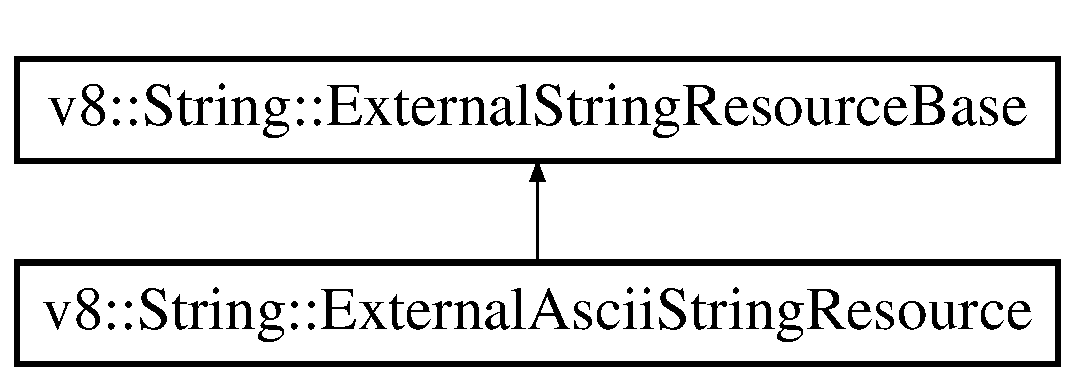
\includegraphics[height=2.000000cm]{classv8_1_1_string_1_1_external_ascii_string_resource}
\end{center}
\end{figure}
\subsection*{Public Member Functions}
\begin{DoxyCompactItemize}
\item 
virtual \hyperlink{classv8_1_1_string_1_1_external_ascii_string_resource_acd8790ae14be1b90794b363d24a147d0}{$\sim$\+External\+Ascii\+String\+Resource} ()
\item 
virtual const char $\ast$ \hyperlink{classv8_1_1_string_1_1_external_ascii_string_resource_adeb99e8c8c630e2dac5ad76476249d2f}{data} () const =0
\item 
virtual size\+\_\+t \hyperlink{classv8_1_1_string_1_1_external_ascii_string_resource_aeecccc52434c2057d3dc5c9732458a8e}{length} () const =0
\end{DoxyCompactItemize}
\subsection*{Additional Inherited Members}


\subsection{Detailed Description}
An \hyperlink{classv8_1_1_string_1_1_external_ascii_string_resource}{External\+Ascii\+String\+Resource} is a wrapper around an ascii string buffer that resides outside \hyperlink{classv8_1_1_v8}{V8}\textquotesingle{}s heap. Implement an \hyperlink{classv8_1_1_string_1_1_external_ascii_string_resource}{External\+Ascii\+String\+Resource} to manage the life cycle of the underlying buffer. Note that the string data must be immutable and that the data must be strict 7-\/bit A\+S\+C\+I\+I, not Latin1 or U\+T\+F-\/8, which would require special treatment internally in the engine and, in the case of U\+T\+F-\/8, do not allow efficient indexing. Use \hyperlink{classv8_1_1_string_af0f9c44d85056bd575c01e8be7cc1b01}{String\+::\+New} or convert to 16 bit data for non-\/\+A\+S\+C\+I\+I. 

\subsection{Constructor \& Destructor Documentation}
\hypertarget{classv8_1_1_string_1_1_external_ascii_string_resource_acd8790ae14be1b90794b363d24a147d0}{}\index{v8\+::\+String\+::\+External\+Ascii\+String\+Resource@{v8\+::\+String\+::\+External\+Ascii\+String\+Resource}!````~External\+Ascii\+String\+Resource@{$\sim$\+External\+Ascii\+String\+Resource}}
\index{````~External\+Ascii\+String\+Resource@{$\sim$\+External\+Ascii\+String\+Resource}!v8\+::\+String\+::\+External\+Ascii\+String\+Resource@{v8\+::\+String\+::\+External\+Ascii\+String\+Resource}}
\subsubsection[{$\sim$\+External\+Ascii\+String\+Resource}]{\setlength{\rightskip}{0pt plus 5cm}virtual v8\+::\+String\+::\+External\+Ascii\+String\+Resource\+::$\sim$\+External\+Ascii\+String\+Resource (
\begin{DoxyParamCaption}
{}
\end{DoxyParamCaption}
)\hspace{0.3cm}{\ttfamily [inline]}, {\ttfamily [virtual]}}\label{classv8_1_1_string_1_1_external_ascii_string_resource_acd8790ae14be1b90794b363d24a147d0}
Override the destructor to manage the life cycle of the underlying buffer. 

\subsection{Member Function Documentation}
\hypertarget{classv8_1_1_string_1_1_external_ascii_string_resource_adeb99e8c8c630e2dac5ad76476249d2f}{}\index{v8\+::\+String\+::\+External\+Ascii\+String\+Resource@{v8\+::\+String\+::\+External\+Ascii\+String\+Resource}!data@{data}}
\index{data@{data}!v8\+::\+String\+::\+External\+Ascii\+String\+Resource@{v8\+::\+String\+::\+External\+Ascii\+String\+Resource}}
\subsubsection[{data}]{\setlength{\rightskip}{0pt plus 5cm}virtual const char$\ast$ v8\+::\+String\+::\+External\+Ascii\+String\+Resource\+::data (
\begin{DoxyParamCaption}
{}
\end{DoxyParamCaption}
) const\hspace{0.3cm}{\ttfamily [pure virtual]}}\label{classv8_1_1_string_1_1_external_ascii_string_resource_adeb99e8c8c630e2dac5ad76476249d2f}
The string data from the underlying buffer. \hypertarget{classv8_1_1_string_1_1_external_ascii_string_resource_aeecccc52434c2057d3dc5c9732458a8e}{}\index{v8\+::\+String\+::\+External\+Ascii\+String\+Resource@{v8\+::\+String\+::\+External\+Ascii\+String\+Resource}!length@{length}}
\index{length@{length}!v8\+::\+String\+::\+External\+Ascii\+String\+Resource@{v8\+::\+String\+::\+External\+Ascii\+String\+Resource}}
\subsubsection[{length}]{\setlength{\rightskip}{0pt plus 5cm}virtual size\+\_\+t v8\+::\+String\+::\+External\+Ascii\+String\+Resource\+::length (
\begin{DoxyParamCaption}
{}
\end{DoxyParamCaption}
) const\hspace{0.3cm}{\ttfamily [pure virtual]}}\label{classv8_1_1_string_1_1_external_ascii_string_resource_aeecccc52434c2057d3dc5c9732458a8e}
The number of ascii characters in the string. 

The documentation for this class was generated from the following file\+:\begin{DoxyCompactItemize}
\item 
deps/v8/include/v8.\+h\end{DoxyCompactItemize}

\hypertarget{classv8_1_1_string_1_1_external_string_resource}{}\section{v8\+:\+:String\+:\+:External\+String\+Resource Class Reference}
\label{classv8_1_1_string_1_1_external_string_resource}\index{v8\+::\+String\+::\+External\+String\+Resource@{v8\+::\+String\+::\+External\+String\+Resource}}


{\ttfamily \#include $<$v8.\+h$>$}

Inheritance diagram for v8\+:\+:String\+:\+:External\+String\+Resource\+:\begin{figure}[H]
\begin{center}
\leavevmode
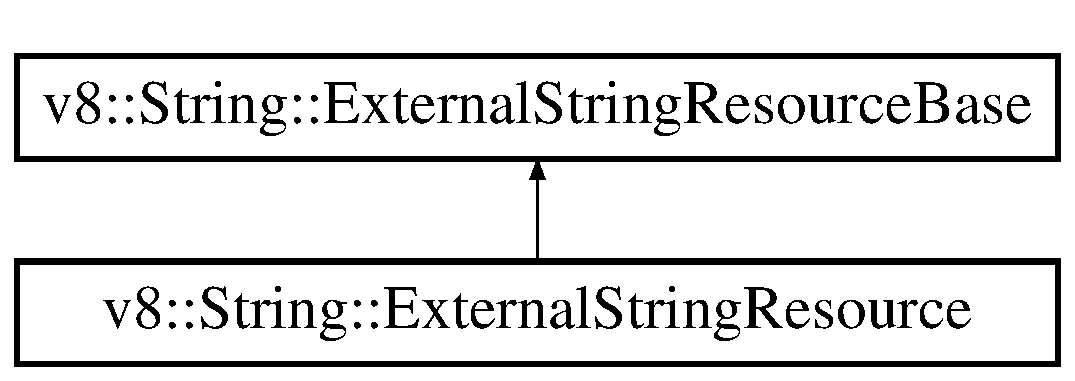
\includegraphics[height=2.000000cm]{classv8_1_1_string_1_1_external_string_resource}
\end{center}
\end{figure}
\subsection*{Public Member Functions}
\begin{DoxyCompactItemize}
\item 
virtual \hyperlink{classv8_1_1_string_1_1_external_string_resource_a6b7ef9e33a47059092e1447b10c35416}{$\sim$\+External\+String\+Resource} ()
\item 
virtual const uint16\+\_\+t $\ast$ \hyperlink{classv8_1_1_string_1_1_external_string_resource_a987309199b848511adb708e221e0fb0a}{data} () const =0
\item 
virtual size\+\_\+t \hyperlink{classv8_1_1_string_1_1_external_string_resource_ab5ca300fea077d7c7774ec49d32e4da1}{length} () const =0
\end{DoxyCompactItemize}
\subsection*{Additional Inherited Members}


\subsection{Detailed Description}
An \hyperlink{classv8_1_1_string_1_1_external_string_resource}{External\+String\+Resource} is a wrapper around a two-\/byte string buffer that resides outside \hyperlink{classv8_1_1_v8}{V8}\textquotesingle{}s heap. Implement an \hyperlink{classv8_1_1_string_1_1_external_string_resource}{External\+String\+Resource} to manage the life cycle of the underlying buffer. Note that the string data must be immutable. 

\subsection{Constructor \& Destructor Documentation}
\hypertarget{classv8_1_1_string_1_1_external_string_resource_a6b7ef9e33a47059092e1447b10c35416}{}\index{v8\+::\+String\+::\+External\+String\+Resource@{v8\+::\+String\+::\+External\+String\+Resource}!````~External\+String\+Resource@{$\sim$\+External\+String\+Resource}}
\index{````~External\+String\+Resource@{$\sim$\+External\+String\+Resource}!v8\+::\+String\+::\+External\+String\+Resource@{v8\+::\+String\+::\+External\+String\+Resource}}
\subsubsection[{$\sim$\+External\+String\+Resource}]{\setlength{\rightskip}{0pt plus 5cm}virtual v8\+::\+String\+::\+External\+String\+Resource\+::$\sim$\+External\+String\+Resource (
\begin{DoxyParamCaption}
{}
\end{DoxyParamCaption}
)\hspace{0.3cm}{\ttfamily [inline]}, {\ttfamily [virtual]}}\label{classv8_1_1_string_1_1_external_string_resource_a6b7ef9e33a47059092e1447b10c35416}
Override the destructor to manage the life cycle of the underlying buffer. 

\subsection{Member Function Documentation}
\hypertarget{classv8_1_1_string_1_1_external_string_resource_a987309199b848511adb708e221e0fb0a}{}\index{v8\+::\+String\+::\+External\+String\+Resource@{v8\+::\+String\+::\+External\+String\+Resource}!data@{data}}
\index{data@{data}!v8\+::\+String\+::\+External\+String\+Resource@{v8\+::\+String\+::\+External\+String\+Resource}}
\subsubsection[{data}]{\setlength{\rightskip}{0pt plus 5cm}virtual const uint16\+\_\+t$\ast$ v8\+::\+String\+::\+External\+String\+Resource\+::data (
\begin{DoxyParamCaption}
{}
\end{DoxyParamCaption}
) const\hspace{0.3cm}{\ttfamily [pure virtual]}}\label{classv8_1_1_string_1_1_external_string_resource_a987309199b848511adb708e221e0fb0a}
The string data from the underlying buffer. \hypertarget{classv8_1_1_string_1_1_external_string_resource_ab5ca300fea077d7c7774ec49d32e4da1}{}\index{v8\+::\+String\+::\+External\+String\+Resource@{v8\+::\+String\+::\+External\+String\+Resource}!length@{length}}
\index{length@{length}!v8\+::\+String\+::\+External\+String\+Resource@{v8\+::\+String\+::\+External\+String\+Resource}}
\subsubsection[{length}]{\setlength{\rightskip}{0pt plus 5cm}virtual size\+\_\+t v8\+::\+String\+::\+External\+String\+Resource\+::length (
\begin{DoxyParamCaption}
{}
\end{DoxyParamCaption}
) const\hspace{0.3cm}{\ttfamily [pure virtual]}}\label{classv8_1_1_string_1_1_external_string_resource_ab5ca300fea077d7c7774ec49d32e4da1}
The length of the string. That is, the number of two-\/byte characters. 

The documentation for this class was generated from the following file\+:\begin{DoxyCompactItemize}
\item 
deps/v8/include/v8.\+h\end{DoxyCompactItemize}

\hypertarget{classv8_1_1_string_1_1_external_string_resource_base}{}\section{v8\+:\+:String\+:\+:External\+String\+Resource\+Base Class Reference}
\label{classv8_1_1_string_1_1_external_string_resource_base}\index{v8\+::\+String\+::\+External\+String\+Resource\+Base@{v8\+::\+String\+::\+External\+String\+Resource\+Base}}
Inheritance diagram for v8\+:\+:String\+:\+:External\+String\+Resource\+Base\+:\begin{figure}[H]
\begin{center}
\leavevmode
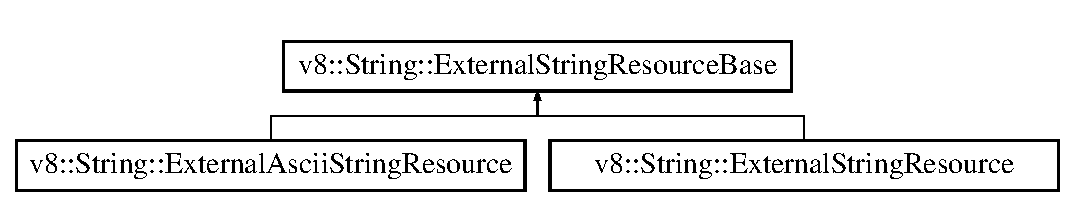
\includegraphics[height=2.000000cm]{classv8_1_1_string_1_1_external_string_resource_base}
\end{center}
\end{figure}


The documentation for this class was generated from the following file\+:\begin{DoxyCompactItemize}
\item 
deps/v8/include/v8.\+h\end{DoxyCompactItemize}

\hypertarget{classv8_1_1_function}{}\section{v8\+:\+:Function Class Reference}
\label{classv8_1_1_function}\index{v8\+::\+Function@{v8\+::\+Function}}


{\ttfamily \#include $<$v8.\+h$>$}

Inheritance diagram for v8\+:\+:Function\+:\begin{figure}[H]
\begin{center}
\leavevmode
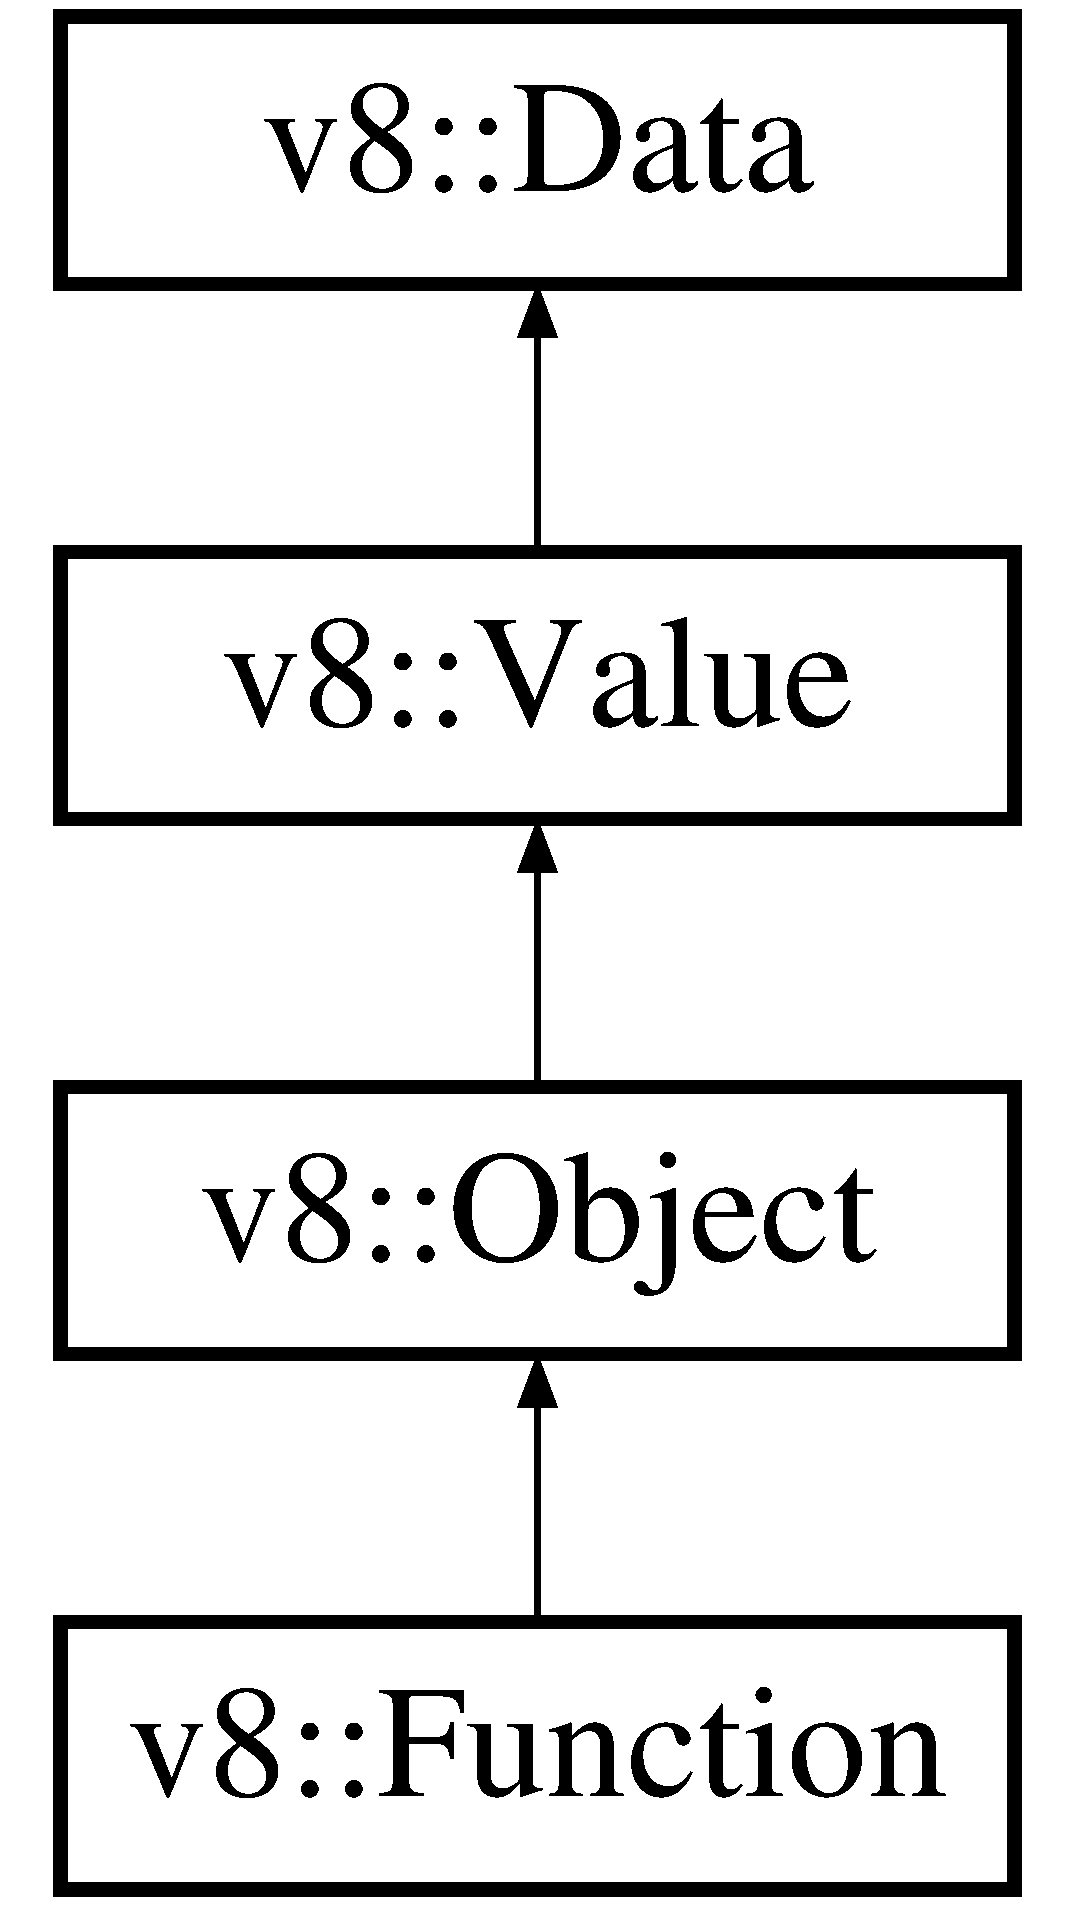
\includegraphics[height=4.000000cm]{classv8_1_1_function}
\end{center}
\end{figure}
\subsection*{Public Member Functions}
\begin{DoxyCompactItemize}
\item 
\hypertarget{classv8_1_1_function_a2bbac81200b840cbd484679aaa5b03d4}{}\hyperlink{classv8_1_1_local}{Local}$<$ \hyperlink{classv8_1_1_object}{Object} $>$ {\bfseries New\+Instance} () const \label{classv8_1_1_function_a2bbac81200b840cbd484679aaa5b03d4}

\item 
\hypertarget{classv8_1_1_function_a1261371c01bf18be5564f290af22e9d9}{}\hyperlink{classv8_1_1_local}{Local}$<$ \hyperlink{classv8_1_1_object}{Object} $>$ {\bfseries New\+Instance} (int argc, \hyperlink{classv8_1_1_handle}{Handle}$<$ \hyperlink{classv8_1_1_value}{Value} $>$ argv\mbox{[}$\,$\mbox{]}) const \label{classv8_1_1_function_a1261371c01bf18be5564f290af22e9d9}

\item 
\hypertarget{classv8_1_1_function_a09b1a95dcd397bfad9d39942605dc3ce}{}\hyperlink{classv8_1_1_local}{Local}$<$ \hyperlink{classv8_1_1_value}{Value} $>$ {\bfseries Call} (\hyperlink{classv8_1_1_handle}{Handle}$<$ \hyperlink{classv8_1_1_value}{Value} $>$ recv, int argc, \hyperlink{classv8_1_1_handle}{Handle}$<$ \hyperlink{classv8_1_1_value}{Value} $>$ argv\mbox{[}$\,$\mbox{]})\label{classv8_1_1_function_a09b1a95dcd397bfad9d39942605dc3ce}

\item 
\hypertarget{classv8_1_1_function_a5e244ce13d6f30ffa69f520126ada795}{}void {\bfseries Set\+Name} (\hyperlink{classv8_1_1_handle}{Handle}$<$ \hyperlink{classv8_1_1_string}{String} $>$ name)\label{classv8_1_1_function_a5e244ce13d6f30ffa69f520126ada795}

\item 
\hypertarget{classv8_1_1_function_adbbf95a036859381c06af3d05cd74b07}{}\hyperlink{classv8_1_1_handle}{Handle}$<$ \hyperlink{classv8_1_1_value}{Value} $>$ {\bfseries Get\+Name} () const \label{classv8_1_1_function_adbbf95a036859381c06af3d05cd74b07}

\item 
\hyperlink{classv8_1_1_handle}{Handle}$<$ \hyperlink{classv8_1_1_value}{Value} $>$ \hyperlink{classv8_1_1_function_a5bd3ad2f8144be5d9b383b1cd9b30df5}{Get\+Inferred\+Name} () const 
\item 
\hyperlink{classv8_1_1_handle}{Handle}$<$ \hyperlink{classv8_1_1_value}{Value} $>$ \hyperlink{classv8_1_1_function_a02e860b1d4f1b58a0c437fec8ea9e290}{Get\+Display\+Name} () const 
\item 
int \hyperlink{classv8_1_1_function_ae64de1b9dc1ea5dc4f419a88808c12c5}{Get\+Script\+Line\+Number} () const 
\item 
int \hyperlink{classv8_1_1_function_abfe6a9251c5dfc995b83dcf3032fdc86}{Get\+Script\+Column\+Number} () const 
\item 
bool \hyperlink{classv8_1_1_function_a4279e2bfca281cda9afdaf86c87d644d}{Is\+Builtin} () const 
\item 
int \hyperlink{classv8_1_1_function_afa208e62e702f6d61ba0a4250ba3f2cf}{Script\+Id} () const 
\item 
\hyperlink{classv8_1_1_local}{Local}$<$ \hyperlink{classv8_1_1_value}{Value} $>$ \hyperlink{classv8_1_1_function_a937dc089e1ef728eec4a628072250e4d}{Get\+Bound\+Function} () const 
\item 
\hypertarget{classv8_1_1_function_af9c77c9bcbf698727071c7153e7c2513}{}\hyperlink{classv8_1_1_script_origin}{Script\+Origin} {\bfseries Get\+Script\+Origin} () const \label{classv8_1_1_function_af9c77c9bcbf698727071c7153e7c2513}

\end{DoxyCompactItemize}
\subsection*{Static Public Member Functions}
\begin{DoxyCompactItemize}
\item 
static \hyperlink{classv8_1_1_local}{Local}$<$ \hyperlink{classv8_1_1_function}{Function} $>$ \hyperlink{classv8_1_1_function_a56e303d1019aaa7954de668aee8486f7}{New} (\hyperlink{classv8_1_1_isolate}{Isolate} $\ast$isolate, Function\+Callback callback, \hyperlink{classv8_1_1_local}{Local}$<$ \hyperlink{classv8_1_1_value}{Value} $>$ data=\hyperlink{classv8_1_1_local}{Local}$<$ \hyperlink{classv8_1_1_value}{Value} $>$(), int length=0)
\item 
\hypertarget{classv8_1_1_function_af24f38bcc0769519816cda1f6a154ff8}{}static V8\+\_\+\+I\+N\+L\+I\+N\+E \hyperlink{classv8_1_1_function}{Function} $\ast$ {\bfseries Cast} (\hyperlink{classv8_1_1_value}{Value} $\ast$obj)\label{classv8_1_1_function_af24f38bcc0769519816cda1f6a154ff8}

\end{DoxyCompactItemize}
\subsection*{Static Public Attributes}
\begin{DoxyCompactItemize}
\item 
\hypertarget{classv8_1_1_function_acf0af24f79908e405a6ac435277596d9}{}static const int {\bfseries k\+Line\+Offset\+Not\+Found}\label{classv8_1_1_function_acf0af24f79908e405a6ac435277596d9}

\end{DoxyCompactItemize}


\subsection{Detailed Description}
A Java\+Script function object (E\+C\+M\+A-\/262, 15.\+3). 

\subsection{Member Function Documentation}
\hypertarget{classv8_1_1_function_a937dc089e1ef728eec4a628072250e4d}{}\index{v8\+::\+Function@{v8\+::\+Function}!Get\+Bound\+Function@{Get\+Bound\+Function}}
\index{Get\+Bound\+Function@{Get\+Bound\+Function}!v8\+::\+Function@{v8\+::\+Function}}
\subsubsection[{Get\+Bound\+Function}]{\setlength{\rightskip}{0pt plus 5cm}{\bf Local}$<${\bf Value}$>$ v8\+::\+Function\+::\+Get\+Bound\+Function (
\begin{DoxyParamCaption}
{}
\end{DoxyParamCaption}
) const}\label{classv8_1_1_function_a937dc089e1ef728eec4a628072250e4d}
Returns the original function if this function is bound, else returns v8\+::\+Undefined. \hypertarget{classv8_1_1_function_a02e860b1d4f1b58a0c437fec8ea9e290}{}\index{v8\+::\+Function@{v8\+::\+Function}!Get\+Display\+Name@{Get\+Display\+Name}}
\index{Get\+Display\+Name@{Get\+Display\+Name}!v8\+::\+Function@{v8\+::\+Function}}
\subsubsection[{Get\+Display\+Name}]{\setlength{\rightskip}{0pt plus 5cm}{\bf Handle}$<${\bf Value}$>$ v8\+::\+Function\+::\+Get\+Display\+Name (
\begin{DoxyParamCaption}
{}
\end{DoxyParamCaption}
) const}\label{classv8_1_1_function_a02e860b1d4f1b58a0c437fec8ea9e290}
User-\/defined name assigned to the \char`\"{}display\+Name\char`\"{} property of this function. Used to facilitate debugging and profiling of Java\+Script code. \hypertarget{classv8_1_1_function_a5bd3ad2f8144be5d9b383b1cd9b30df5}{}\index{v8\+::\+Function@{v8\+::\+Function}!Get\+Inferred\+Name@{Get\+Inferred\+Name}}
\index{Get\+Inferred\+Name@{Get\+Inferred\+Name}!v8\+::\+Function@{v8\+::\+Function}}
\subsubsection[{Get\+Inferred\+Name}]{\setlength{\rightskip}{0pt plus 5cm}{\bf Handle}$<${\bf Value}$>$ v8\+::\+Function\+::\+Get\+Inferred\+Name (
\begin{DoxyParamCaption}
{}
\end{DoxyParamCaption}
) const}\label{classv8_1_1_function_a5bd3ad2f8144be5d9b383b1cd9b30df5}
\hyperlink{classv8_1_1_name}{Name} inferred from variable or property assignment of this function. Used to facilitate debugging and profiling of Java\+Script code written in an O\+O style, where many functions are anonymous but are assigned to object properties. \hypertarget{classv8_1_1_function_abfe6a9251c5dfc995b83dcf3032fdc86}{}\index{v8\+::\+Function@{v8\+::\+Function}!Get\+Script\+Column\+Number@{Get\+Script\+Column\+Number}}
\index{Get\+Script\+Column\+Number@{Get\+Script\+Column\+Number}!v8\+::\+Function@{v8\+::\+Function}}
\subsubsection[{Get\+Script\+Column\+Number}]{\setlength{\rightskip}{0pt plus 5cm}int v8\+::\+Function\+::\+Get\+Script\+Column\+Number (
\begin{DoxyParamCaption}
{}
\end{DoxyParamCaption}
) const}\label{classv8_1_1_function_abfe6a9251c5dfc995b83dcf3032fdc86}
Returns zero based column number of function body and k\+Line\+Offset\+Not\+Found if no information available. \hypertarget{classv8_1_1_function_ae64de1b9dc1ea5dc4f419a88808c12c5}{}\index{v8\+::\+Function@{v8\+::\+Function}!Get\+Script\+Line\+Number@{Get\+Script\+Line\+Number}}
\index{Get\+Script\+Line\+Number@{Get\+Script\+Line\+Number}!v8\+::\+Function@{v8\+::\+Function}}
\subsubsection[{Get\+Script\+Line\+Number}]{\setlength{\rightskip}{0pt plus 5cm}int v8\+::\+Function\+::\+Get\+Script\+Line\+Number (
\begin{DoxyParamCaption}
{}
\end{DoxyParamCaption}
) const}\label{classv8_1_1_function_ae64de1b9dc1ea5dc4f419a88808c12c5}
Returns zero based line number of function body and k\+Line\+Offset\+Not\+Found if no information available. \hypertarget{classv8_1_1_function_a4279e2bfca281cda9afdaf86c87d644d}{}\index{v8\+::\+Function@{v8\+::\+Function}!Is\+Builtin@{Is\+Builtin}}
\index{Is\+Builtin@{Is\+Builtin}!v8\+::\+Function@{v8\+::\+Function}}
\subsubsection[{Is\+Builtin}]{\setlength{\rightskip}{0pt plus 5cm}bool v8\+::\+Function\+::\+Is\+Builtin (
\begin{DoxyParamCaption}
{}
\end{DoxyParamCaption}
) const}\label{classv8_1_1_function_a4279e2bfca281cda9afdaf86c87d644d}
Tells whether this function is builtin. \hypertarget{classv8_1_1_function_a56e303d1019aaa7954de668aee8486f7}{}\index{v8\+::\+Function@{v8\+::\+Function}!New@{New}}
\index{New@{New}!v8\+::\+Function@{v8\+::\+Function}}
\subsubsection[{New}]{\setlength{\rightskip}{0pt plus 5cm}static {\bf Local}$<${\bf Function}$>$ v8\+::\+Function\+::\+New (
\begin{DoxyParamCaption}
\item[{{\bf Isolate} $\ast$}]{isolate, }
\item[{Function\+Callback}]{callback, }
\item[{{\bf Local}$<$ {\bf Value} $>$}]{data = {\ttfamily {\bf Local}$<$~{\bf Value}~$>$()}, }
\item[{int}]{length = {\ttfamily 0}}
\end{DoxyParamCaption}
)\hspace{0.3cm}{\ttfamily [static]}}\label{classv8_1_1_function_a56e303d1019aaa7954de668aee8486f7}
Create a function in the current execution context for a given Function\+Callback. \hypertarget{classv8_1_1_function_afa208e62e702f6d61ba0a4250ba3f2cf}{}\index{v8\+::\+Function@{v8\+::\+Function}!Script\+Id@{Script\+Id}}
\index{Script\+Id@{Script\+Id}!v8\+::\+Function@{v8\+::\+Function}}
\subsubsection[{Script\+Id}]{\setlength{\rightskip}{0pt plus 5cm}int v8\+::\+Function\+::\+Script\+Id (
\begin{DoxyParamCaption}
{}
\end{DoxyParamCaption}
) const}\label{classv8_1_1_function_afa208e62e702f6d61ba0a4250ba3f2cf}
Returns script\+Id. 

The documentation for this class was generated from the following file\+:\begin{DoxyCompactItemize}
\item 
deps/v8/include/v8.\+h\end{DoxyCompactItemize}

\hypertarget{classv8_1_1_function_template}{}\section{v8\+:\+:Function\+Template Class Reference}
\label{classv8_1_1_function_template}\index{v8\+::\+Function\+Template@{v8\+::\+Function\+Template}}


{\ttfamily \#include $<$v8.\+h$>$}

Inheritance diagram for v8\+:\+:Function\+Template\+:\begin{figure}[H]
\begin{center}
\leavevmode
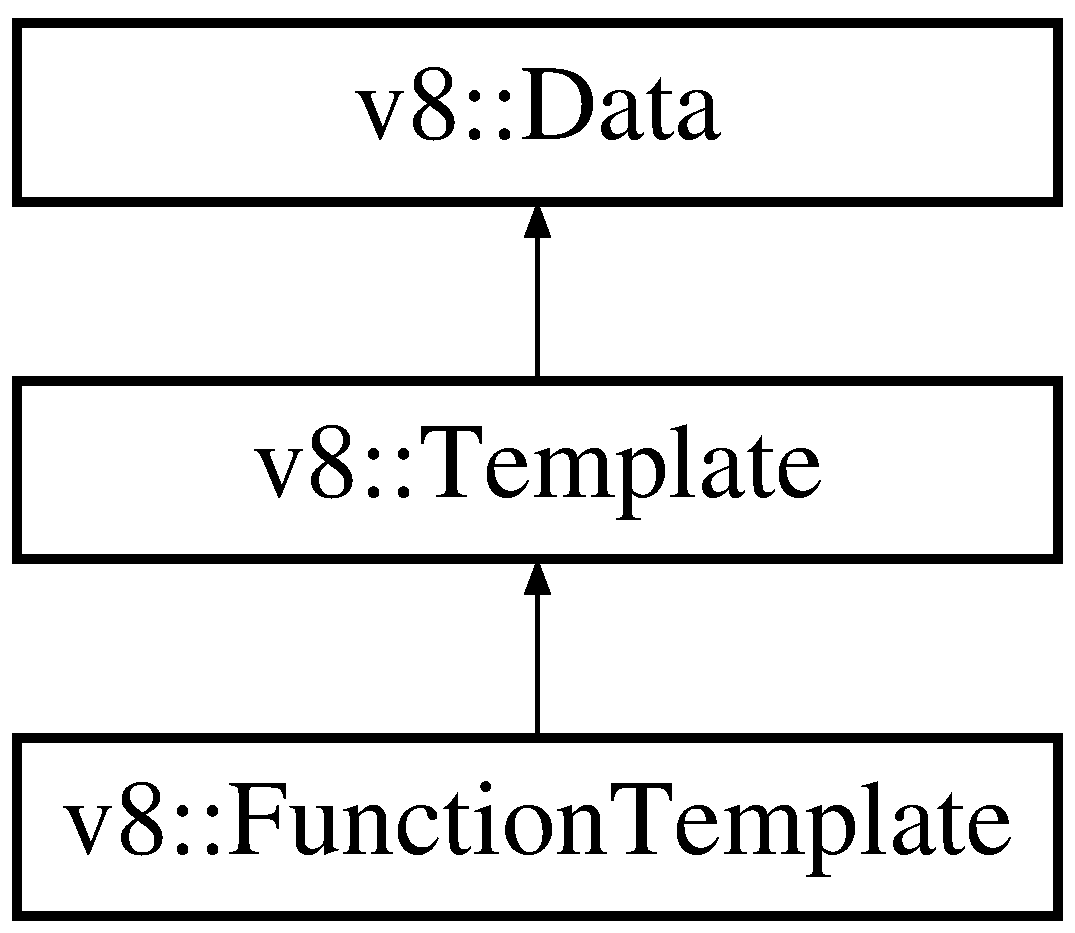
\includegraphics[height=3.000000cm]{classv8_1_1_function_template}
\end{center}
\end{figure}
\subsection*{Public Member Functions}
\begin{DoxyCompactItemize}
\item 
\hyperlink{classv8_1_1_local}{Local}$<$ \hyperlink{classv8_1_1_function}{Function} $>$ \hyperlink{classv8_1_1_function_template_a3b8e5e214b2ee34c36138961ebac696a}{Get\+Function} ()
\item 
void \hyperlink{classv8_1_1_function_template_a9eb1c827b17faf398a81068721bf40ab}{Set\+Call\+Handler} (Invocation\+Callback callback, \hyperlink{classv8_1_1_handle}{Handle}$<$ \hyperlink{classv8_1_1_value}{Value} $>$ data=\hyperlink{classv8_1_1_handle}{Handle}$<$ \hyperlink{classv8_1_1_value}{Value} $>$())
\item 
\hyperlink{classv8_1_1_local}{Local}$<$ \hyperlink{classv8_1_1_object_template}{Object\+Template} $>$ \hyperlink{classv8_1_1_function_template_a00dd9725566908e8fd14064542f5a781}{Instance\+Template} ()
\item 
void \hyperlink{classv8_1_1_function_template_a18f343e7e5749ed886d6e76a1424216e}{Inherit} (\hyperlink{classv8_1_1_handle}{Handle}$<$ \hyperlink{classv8_1_1_function_template}{Function\+Template} $>$ parent)
\item 
\hyperlink{classv8_1_1_local}{Local}$<$ \hyperlink{classv8_1_1_object_template}{Object\+Template} $>$ \hyperlink{classv8_1_1_function_template_aa2bcc2652b5f0fdbc666d943ccf72021}{Prototype\+Template} ()
\item 
void \hyperlink{classv8_1_1_function_template_a10ad6f0d3d1f67823e08fbca7c5dde41}{Set\+Class\+Name} (\hyperlink{classv8_1_1_handle}{Handle}$<$ \hyperlink{classv8_1_1_string}{String} $>$ name)
\item 
void \hyperlink{classv8_1_1_function_template_ade426e8a21d777ae6100e6c1aa7bfaee}{Set\+Hidden\+Prototype} (bool value)
\item 
void \hyperlink{classv8_1_1_function_template_a91d2e0643e8c5a53ab1d75f7766c2422}{Read\+Only\+Prototype} ()
\item 
bool \hyperlink{classv8_1_1_function_template_aa883e4ab6643498662f7873506098c98}{Has\+Instance} (\hyperlink{classv8_1_1_handle}{Handle}$<$ \hyperlink{classv8_1_1_value}{Value} $>$ object)
\end{DoxyCompactItemize}
\subsection*{Static Public Member Functions}
\begin{DoxyCompactItemize}
\item 
static \hyperlink{classv8_1_1_local}{Local}$<$ \hyperlink{classv8_1_1_function_template}{Function\+Template} $>$ \hyperlink{classv8_1_1_function_template_af9012aee4a102c4018fec8e9532cb996}{New} (Invocation\+Callback callback=0, \hyperlink{classv8_1_1_handle}{Handle}$<$ \hyperlink{classv8_1_1_value}{Value} $>$ data=\hyperlink{classv8_1_1_handle}{Handle}$<$ \hyperlink{classv8_1_1_value}{Value} $>$(), \hyperlink{classv8_1_1_handle}{Handle}$<$ \hyperlink{classv8_1_1_signature}{Signature} $>$ signature=\hyperlink{classv8_1_1_handle}{Handle}$<$ \hyperlink{classv8_1_1_signature}{Signature} $>$())
\end{DoxyCompactItemize}
\subsection*{Friends}
\begin{DoxyCompactItemize}
\item 
\hypertarget{classv8_1_1_function_template_ac26c806e60ca4a0547680edb68f6e39b}{}class {\bfseries Context}\label{classv8_1_1_function_template_ac26c806e60ca4a0547680edb68f6e39b}

\item 
\hypertarget{classv8_1_1_function_template_a4d28646409234f556983be8a96c06424}{}class {\bfseries Object\+Template}\label{classv8_1_1_function_template_a4d28646409234f556983be8a96c06424}

\end{DoxyCompactItemize}


\subsection{Detailed Description}
A \hyperlink{classv8_1_1_function_template}{Function\+Template} is used to create functions at runtime. There can only be one function created from a \hyperlink{classv8_1_1_function_template}{Function\+Template} in a context. The lifetime of the created function is equal to the lifetime of the context. So in case the embedder needs to create temporary functions that can be collected using Scripts is preferred.

A \hyperlink{classv8_1_1_function_template}{Function\+Template} can have properties, these properties are added to the function object when it is created.

A \hyperlink{classv8_1_1_function_template}{Function\+Template} has a corresponding instance template which is used to create object instances when the function is used as a constructor. Properties added to the instance template are added to each object instance.

A \hyperlink{classv8_1_1_function_template}{Function\+Template} can have a prototype template. The prototype template is used to create the prototype object of the function.

The following example shows how to use a \hyperlink{classv8_1_1_function_template}{Function\+Template}\+:


\begin{DoxyCode}
\hyperlink{classv8_1_1_local}{v8::Local<v8::FunctionTemplate>} t = 
      \hyperlink{classv8_1_1_function_template_af9012aee4a102c4018fec8e9532cb996}{v8::FunctionTemplate::New}();
t->\hyperlink{classv8_1_1_template_a8a29557db5d0bc980752084b925a9b01}{Set}(\textcolor{stringliteral}{"func\_property"}, v8::Number::New(1));

\hyperlink{classv8_1_1_local}{v8::Local<v8::Template>} proto\_t = t->\hyperlink{classv8_1_1_function_template_aa2bcc2652b5f0fdbc666d943ccf72021}{PrototypeTemplate}();
proto\_t->\hyperlink{classv8_1_1_template_a8a29557db5d0bc980752084b925a9b01}{Set}(\textcolor{stringliteral}{"proto\_method"}, \hyperlink{classv8_1_1_function_template_af9012aee4a102c4018fec8e9532cb996}{v8::FunctionTemplate::New}(InvokeCallback));
proto\_t->\hyperlink{classv8_1_1_template_a8a29557db5d0bc980752084b925a9b01}{Set}(\textcolor{stringliteral}{"proto\_const"}, v8::Number::New(2));

\hyperlink{classv8_1_1_local}{v8::Local<v8::ObjectTemplate>} instance\_t = t->
      \hyperlink{classv8_1_1_function_template_a00dd9725566908e8fd14064542f5a781}{InstanceTemplate}();
instance\_t->\hyperlink{classv8_1_1_object_template_a912ade2f7db7c7e30b606d10012c2bac}{SetAccessor}(\textcolor{stringliteral}{"instance\_accessor"}, InstanceAccessorCallback);
instance\_t->\hyperlink{classv8_1_1_object_template_aa80e9db593d8b954c4153082dc7a439d}{SetNamedPropertyHandler}(PropertyHandlerCallback, ...);
instance\_t->\hyperlink{classv8_1_1_template_a8a29557db5d0bc980752084b925a9b01}{Set}(\textcolor{stringliteral}{"instance\_property"}, Number::New(3));

\hyperlink{classv8_1_1_local}{v8::Local<v8::Function>} \textcolor{keyword}{function} = t->\hyperlink{classv8_1_1_function_template_a3b8e5e214b2ee34c36138961ebac696a}{GetFunction}();
\hyperlink{classv8_1_1_local}{v8::Local<v8::Object>} instance = \textcolor{keyword}{function}->NewInstance();
\end{DoxyCode}


Let\textquotesingle{}s use \char`\"{}function\char`\"{} as the J\+S variable name of the function object and \char`\"{}instance\char`\"{} for the instance object created above. The function and the instance will have the following properties\+:


\begin{DoxyCode}
func\_property in \textcolor{keyword}{function} == \textcolor{keyword}{true};
\textcolor{keyword}{function}.func\_property == 1;

\textcolor{keyword}{function}.prototype.proto\_method() invokes \textcolor{stringliteral}{'InvokeCallback'}
\textcolor{keyword}{function}.prototype.proto\_const == 2;

instance instanceof \textcolor{keyword}{function} == \textcolor{keyword}{true};
instance.instance\_accessor calls \textcolor{stringliteral}{'InstanceAccessorCallback'}
instance.instance\_property == 3;
\end{DoxyCode}


A \hyperlink{classv8_1_1_function_template}{Function\+Template} can inherit from another one by calling the \hyperlink{classv8_1_1_function_template_a18f343e7e5749ed886d6e76a1424216e}{Function\+Template\+::\+Inherit} method. The following graph illustrates the semantics of inheritance\+:


\begin{DoxyCode}
FunctionTemplate Parent  -> Parent() . prototype -> \{ \}
  ^                                                  ^
  | \hyperlink{classv8_1_1_function_template_a18f343e7e5749ed886d6e76a1424216e}{Inherit}(Parent)                                  | .\_\_proto\_\_
  |                                                  |
FunctionTemplate Child   -> Child()  . prototype -> \{ \}
\end{DoxyCode}


A \hyperlink{classv8_1_1_function_template}{Function\+Template} \textquotesingle{}Child\textquotesingle{} inherits from \textquotesingle{}Parent\textquotesingle{}, the prototype object of the Child() function has {\bfseries proto} pointing to the Parent() function\textquotesingle{}s prototype object. An instance of the Child function has all properties on Parent\textquotesingle{}s instance templates.

Let Parent be the \hyperlink{classv8_1_1_function_template}{Function\+Template} initialized in the previous section and create a Child \hyperlink{classv8_1_1_function_template}{Function\+Template} by\+:


\begin{DoxyCode}
Local<FunctionTemplate> parent = t;
Local<FunctionTemplate> child = \hyperlink{classv8_1_1_function_template_af9012aee4a102c4018fec8e9532cb996}{FunctionTemplate::New}();
child->Inherit(parent);

Local<Function> child\_function = child->GetFunction();
Local<Object> child\_instance = child\_function->NewInstance();
\end{DoxyCode}


The Child function and Child instance will have the following properties\+:


\begin{DoxyCode}
child\_func.prototype.\_\_proto\_\_ == \textcolor{keyword}{function}.prototype;
child\_instance.instance\_accessor calls \textcolor{stringliteral}{'InstanceAccessorCallback'}
child\_instance.instance\_property == 3;
\end{DoxyCode}
 

\subsection{Member Function Documentation}
\hypertarget{classv8_1_1_function_template_a3b8e5e214b2ee34c36138961ebac696a}{}\index{v8\+::\+Function\+Template@{v8\+::\+Function\+Template}!Get\+Function@{Get\+Function}}
\index{Get\+Function@{Get\+Function}!v8\+::\+Function\+Template@{v8\+::\+Function\+Template}}
\subsubsection[{Get\+Function}]{\setlength{\rightskip}{0pt plus 5cm}{\bf Local}$<${\bf Function}$>$ v8\+::\+Function\+Template\+::\+Get\+Function (
\begin{DoxyParamCaption}
{}
\end{DoxyParamCaption}
)}\label{classv8_1_1_function_template_a3b8e5e214b2ee34c36138961ebac696a}
Returns the unique function instance in the current execution context. \hypertarget{classv8_1_1_function_template_aa883e4ab6643498662f7873506098c98}{}\index{v8\+::\+Function\+Template@{v8\+::\+Function\+Template}!Has\+Instance@{Has\+Instance}}
\index{Has\+Instance@{Has\+Instance}!v8\+::\+Function\+Template@{v8\+::\+Function\+Template}}
\subsubsection[{Has\+Instance}]{\setlength{\rightskip}{0pt plus 5cm}bool v8\+::\+Function\+Template\+::\+Has\+Instance (
\begin{DoxyParamCaption}
\item[{{\bf Handle}$<$ {\bf Value} $>$}]{object}
\end{DoxyParamCaption}
)}\label{classv8_1_1_function_template_aa883e4ab6643498662f7873506098c98}
Returns true if the given object is an instance of this function template. \hypertarget{classv8_1_1_function_template_a18f343e7e5749ed886d6e76a1424216e}{}\index{v8\+::\+Function\+Template@{v8\+::\+Function\+Template}!Inherit@{Inherit}}
\index{Inherit@{Inherit}!v8\+::\+Function\+Template@{v8\+::\+Function\+Template}}
\subsubsection[{Inherit}]{\setlength{\rightskip}{0pt plus 5cm}void v8\+::\+Function\+Template\+::\+Inherit (
\begin{DoxyParamCaption}
\item[{{\bf Handle}$<$ {\bf Function\+Template} $>$}]{parent}
\end{DoxyParamCaption}
)}\label{classv8_1_1_function_template_a18f343e7e5749ed886d6e76a1424216e}
Causes the function template to inherit from a parent function template. \hypertarget{classv8_1_1_function_template_a00dd9725566908e8fd14064542f5a781}{}\index{v8\+::\+Function\+Template@{v8\+::\+Function\+Template}!Instance\+Template@{Instance\+Template}}
\index{Instance\+Template@{Instance\+Template}!v8\+::\+Function\+Template@{v8\+::\+Function\+Template}}
\subsubsection[{Instance\+Template}]{\setlength{\rightskip}{0pt plus 5cm}{\bf Local}$<${\bf Object\+Template}$>$ v8\+::\+Function\+Template\+::\+Instance\+Template (
\begin{DoxyParamCaption}
{}
\end{DoxyParamCaption}
)}\label{classv8_1_1_function_template_a00dd9725566908e8fd14064542f5a781}
Get the Instance\+Template. \hypertarget{classv8_1_1_function_template_af9012aee4a102c4018fec8e9532cb996}{}\index{v8\+::\+Function\+Template@{v8\+::\+Function\+Template}!New@{New}}
\index{New@{New}!v8\+::\+Function\+Template@{v8\+::\+Function\+Template}}
\subsubsection[{New}]{\setlength{\rightskip}{0pt plus 5cm}static {\bf Local}$<${\bf Function\+Template}$>$ v8\+::\+Function\+Template\+::\+New (
\begin{DoxyParamCaption}
\item[{Invocation\+Callback}]{callback = {\ttfamily 0}, }
\item[{{\bf Handle}$<$ {\bf Value} $>$}]{data = {\ttfamily {\bf Handle}$<$~{\bf Value}~$>$()}, }
\item[{{\bf Handle}$<$ {\bf Signature} $>$}]{signature = {\ttfamily {\bf Handle}$<$~{\bf Signature}~$>$()}}
\end{DoxyParamCaption}
)\hspace{0.3cm}{\ttfamily [static]}}\label{classv8_1_1_function_template_af9012aee4a102c4018fec8e9532cb996}
Creates a function template. \hypertarget{classv8_1_1_function_template_aa2bcc2652b5f0fdbc666d943ccf72021}{}\index{v8\+::\+Function\+Template@{v8\+::\+Function\+Template}!Prototype\+Template@{Prototype\+Template}}
\index{Prototype\+Template@{Prototype\+Template}!v8\+::\+Function\+Template@{v8\+::\+Function\+Template}}
\subsubsection[{Prototype\+Template}]{\setlength{\rightskip}{0pt plus 5cm}{\bf Local}$<${\bf Object\+Template}$>$ v8\+::\+Function\+Template\+::\+Prototype\+Template (
\begin{DoxyParamCaption}
{}
\end{DoxyParamCaption}
)}\label{classv8_1_1_function_template_aa2bcc2652b5f0fdbc666d943ccf72021}
A Prototype\+Template is the template used to create the prototype object of the function created by this template. \hypertarget{classv8_1_1_function_template_a91d2e0643e8c5a53ab1d75f7766c2422}{}\index{v8\+::\+Function\+Template@{v8\+::\+Function\+Template}!Read\+Only\+Prototype@{Read\+Only\+Prototype}}
\index{Read\+Only\+Prototype@{Read\+Only\+Prototype}!v8\+::\+Function\+Template@{v8\+::\+Function\+Template}}
\subsubsection[{Read\+Only\+Prototype}]{\setlength{\rightskip}{0pt plus 5cm}void v8\+::\+Function\+Template\+::\+Read\+Only\+Prototype (
\begin{DoxyParamCaption}
{}
\end{DoxyParamCaption}
)}\label{classv8_1_1_function_template_a91d2e0643e8c5a53ab1d75f7766c2422}
Sets the Read\+Only flag in the attributes of the \textquotesingle{}prototype\textquotesingle{} property of functions created from this \hyperlink{classv8_1_1_function_template}{Function\+Template} to true. \hypertarget{classv8_1_1_function_template_a9eb1c827b17faf398a81068721bf40ab}{}\index{v8\+::\+Function\+Template@{v8\+::\+Function\+Template}!Set\+Call\+Handler@{Set\+Call\+Handler}}
\index{Set\+Call\+Handler@{Set\+Call\+Handler}!v8\+::\+Function\+Template@{v8\+::\+Function\+Template}}
\subsubsection[{Set\+Call\+Handler}]{\setlength{\rightskip}{0pt plus 5cm}void v8\+::\+Function\+Template\+::\+Set\+Call\+Handler (
\begin{DoxyParamCaption}
\item[{Invocation\+Callback}]{callback, }
\item[{{\bf Handle}$<$ {\bf Value} $>$}]{data = {\ttfamily {\bf Handle}$<$~{\bf Value}~$>$()}}
\end{DoxyParamCaption}
)}\label{classv8_1_1_function_template_a9eb1c827b17faf398a81068721bf40ab}
Set the call-\/handler callback for a \hyperlink{classv8_1_1_function_template}{Function\+Template}. This callback is called whenever the function created from this \hyperlink{classv8_1_1_function_template}{Function\+Template} is called. \hypertarget{classv8_1_1_function_template_a10ad6f0d3d1f67823e08fbca7c5dde41}{}\index{v8\+::\+Function\+Template@{v8\+::\+Function\+Template}!Set\+Class\+Name@{Set\+Class\+Name}}
\index{Set\+Class\+Name@{Set\+Class\+Name}!v8\+::\+Function\+Template@{v8\+::\+Function\+Template}}
\subsubsection[{Set\+Class\+Name}]{\setlength{\rightskip}{0pt plus 5cm}void v8\+::\+Function\+Template\+::\+Set\+Class\+Name (
\begin{DoxyParamCaption}
\item[{{\bf Handle}$<$ {\bf String} $>$}]{name}
\end{DoxyParamCaption}
)}\label{classv8_1_1_function_template_a10ad6f0d3d1f67823e08fbca7c5dde41}
Set the class name of the \hyperlink{classv8_1_1_function_template}{Function\+Template}. This is used for printing objects created with the function created from the \hyperlink{classv8_1_1_function_template}{Function\+Template} as its constructor. \hypertarget{classv8_1_1_function_template_ade426e8a21d777ae6100e6c1aa7bfaee}{}\index{v8\+::\+Function\+Template@{v8\+::\+Function\+Template}!Set\+Hidden\+Prototype@{Set\+Hidden\+Prototype}}
\index{Set\+Hidden\+Prototype@{Set\+Hidden\+Prototype}!v8\+::\+Function\+Template@{v8\+::\+Function\+Template}}
\subsubsection[{Set\+Hidden\+Prototype}]{\setlength{\rightskip}{0pt plus 5cm}void v8\+::\+Function\+Template\+::\+Set\+Hidden\+Prototype (
\begin{DoxyParamCaption}
\item[{bool}]{value}
\end{DoxyParamCaption}
)}\label{classv8_1_1_function_template_ade426e8a21d777ae6100e6c1aa7bfaee}
Determines whether the {\bfseries proto} accessor ignores instances of the function template. If instances of the function template are ignored, {\bfseries proto} skips all instances and instead returns the next object in the prototype chain.

Call with a value of true to make the {\bfseries proto} accessor ignore instances of the function template. Call with a value of false to make the {\bfseries proto} accessor not ignore instances of the function template. By default, instances of a function template are not ignored. 

The documentation for this class was generated from the following file\+:\begin{DoxyCompactItemize}
\item 
deps/v8/include/v8.\+h\end{DoxyCompactItemize}

\hypertarget{classv8_1_1_handle}{}\section{v8\+:\+:Handle$<$ T $>$ Class Template Reference}
\label{classv8_1_1_handle}\index{v8\+::\+Handle$<$ T $>$@{v8\+::\+Handle$<$ T $>$}}


{\ttfamily \#include $<$v8.\+h$>$}

Inheritance diagram for v8\+:\+:Handle$<$ T $>$\+:\begin{figure}[H]
\begin{center}
\leavevmode
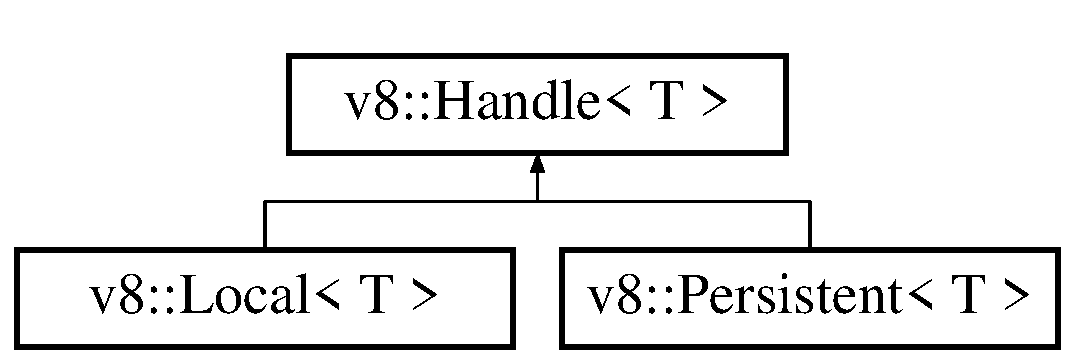
\includegraphics[height=2.000000cm]{classv8_1_1_handle}
\end{center}
\end{figure}
\subsection*{Public Member Functions}
\begin{DoxyCompactItemize}
\item 
\hyperlink{classv8_1_1_handle_aa7543a3d572565806a66e922634cc2f4}{Handle} ()
\item 
\hyperlink{classv8_1_1_handle_aac16277f1131898a4a2ef664d051cc18}{Handle} (T $\ast$val)
\item 
{\footnotesize template$<$class S $>$ }\\\hyperlink{classv8_1_1_handle_a64aee8fcde243c8a5abebfe534b3797a}{Handle} (\hyperlink{classv8_1_1_handle}{Handle}$<$ S $>$ that)
\item 
bool \hyperlink{classv8_1_1_handle_ab3b20b28e7f672de83a2dc8d6809f815}{Is\+Empty} () const 
\item 
\hypertarget{classv8_1_1_handle_af5285c2e91079e380651f83195383228}{}T $\ast$ {\bfseries operator-\/$>$} () const \label{classv8_1_1_handle_af5285c2e91079e380651f83195383228}

\item 
\hypertarget{classv8_1_1_handle_a524a50d9802a97beb1b5e405c6fc6f21}{}T $\ast$ {\bfseries operator$\ast$} () const \label{classv8_1_1_handle_a524a50d9802a97beb1b5e405c6fc6f21}

\item 
void \hyperlink{classv8_1_1_handle_a452516a09df056438c3d3a177ebd1977}{Clear} ()
\item 
{\footnotesize template$<$class S $>$ }\\bool \hyperlink{classv8_1_1_handle_afcc79738c6fff05c70e958a471f2b7d9}{operator==} (\hyperlink{classv8_1_1_handle}{Handle}$<$ S $>$ that) const 
\item 
{\footnotesize template$<$class S $>$ }\\bool \hyperlink{classv8_1_1_handle_ab550353b4a7bc3ad3df53fe80df7ea61}{operator!=} (\hyperlink{classv8_1_1_handle}{Handle}$<$ S $>$ that) const 
\item 
\hypertarget{classv8_1_1_handle_a1cfaea378fc1a419101d4cc02d34e404}{}{\footnotesize template$<$class S $>$ }\\\hyperlink{classv8_1_1_handle}{Handle}$<$ S $>$ {\bfseries As} ()\label{classv8_1_1_handle_a1cfaea378fc1a419101d4cc02d34e404}

\end{DoxyCompactItemize}
\subsection*{Static Public Member Functions}
\begin{DoxyCompactItemize}
\item 
\hypertarget{classv8_1_1_handle_a78abe2e84ab0829779b714feea1bc4d1}{}{\footnotesize template$<$class S $>$ }\\static \hyperlink{classv8_1_1_handle}{Handle}$<$ T $>$ {\bfseries Cast} (\hyperlink{classv8_1_1_handle}{Handle}$<$ S $>$ that)\label{classv8_1_1_handle_a78abe2e84ab0829779b714feea1bc4d1}

\end{DoxyCompactItemize}


\subsection{Detailed Description}
\subsubsection*{template$<$class T$>$class v8\+::\+Handle$<$ T $>$}

An object reference managed by the \hyperlink{namespacev8}{v8} garbage collector.

All objects returned from \hyperlink{namespacev8}{v8} have to be tracked by the garbage collector so that it knows that the objects are still alive. Also, because the garbage collector may move objects, it is unsafe to point directly to an object. Instead, all objects are stored in handles which are known by the garbage collector and updated whenever an object moves. Handles should always be passed by value (except in cases like out-\/parameters) and they should never be allocated on the heap.

There are two types of handles\+: local and persistent handles. \hyperlink{classv8_1_1_local}{Local} handles are light-\/weight and transient and typically used in local operations. They are managed by Handle\+Scopes. \hyperlink{classv8_1_1_persistent}{Persistent} handles can be used when storing objects across several independent operations and have to be explicitly deallocated when they\textquotesingle{}re no longer used.

It is safe to extract the object stored in the handle by dereferencing the handle (for instance, to extract the Object$\ast$ from an Handle$<$\+Object$>$); the value will still be governed by a handle behind the scenes and the same rules apply to these values as to their handles. 

\subsection{Constructor \& Destructor Documentation}
\hypertarget{classv8_1_1_handle_aa7543a3d572565806a66e922634cc2f4}{}\index{v8\+::\+Handle@{v8\+::\+Handle}!Handle@{Handle}}
\index{Handle@{Handle}!v8\+::\+Handle@{v8\+::\+Handle}}
\subsubsection[{Handle}]{\setlength{\rightskip}{0pt plus 5cm}template$<$class T $>$ {\bf v8\+::\+Handle}$<$ T $>$\+::{\bf Handle} (
\begin{DoxyParamCaption}
{}
\end{DoxyParamCaption}
)\hspace{0.3cm}{\ttfamily [inline]}}\label{classv8_1_1_handle_aa7543a3d572565806a66e922634cc2f4}
Creates an empty handle. \hypertarget{classv8_1_1_handle_aac16277f1131898a4a2ef664d051cc18}{}\index{v8\+::\+Handle@{v8\+::\+Handle}!Handle@{Handle}}
\index{Handle@{Handle}!v8\+::\+Handle@{v8\+::\+Handle}}
\subsubsection[{Handle}]{\setlength{\rightskip}{0pt plus 5cm}template$<$class T$>$ {\bf v8\+::\+Handle}$<$ T $>$\+::{\bf Handle} (
\begin{DoxyParamCaption}
\item[{T $\ast$}]{val}
\end{DoxyParamCaption}
)\hspace{0.3cm}{\ttfamily [inline]}, {\ttfamily [explicit]}}\label{classv8_1_1_handle_aac16277f1131898a4a2ef664d051cc18}
Creates a new handle for the specified value. \hypertarget{classv8_1_1_handle_a64aee8fcde243c8a5abebfe534b3797a}{}\index{v8\+::\+Handle@{v8\+::\+Handle}!Handle@{Handle}}
\index{Handle@{Handle}!v8\+::\+Handle@{v8\+::\+Handle}}
\subsubsection[{Handle}]{\setlength{\rightskip}{0pt plus 5cm}template$<$class T$>$ template$<$class S $>$ {\bf v8\+::\+Handle}$<$ T $>$\+::{\bf Handle} (
\begin{DoxyParamCaption}
\item[{{\bf Handle}$<$ S $>$}]{that}
\end{DoxyParamCaption}
)\hspace{0.3cm}{\ttfamily [inline]}}\label{classv8_1_1_handle_a64aee8fcde243c8a5abebfe534b3797a}
Creates a handle for the contents of the specified handle. This constructor allows you to pass handles as arguments by value and to assign between handles. However, if you try to assign between incompatible handles, for instance from a Handle$<$\+String$>$ to a Handle$<$\+Number$>$ it will cause a compiletime error. Assigning between compatible handles, for instance assigning a Handle$<$\+String$>$ to a variable declared as Handle$<$\+Value$>$, is legal because \hyperlink{classv8_1_1_string}{String} is a subclass of \hyperlink{classv8_1_1_value}{Value}. This check fails when trying to convert between incompatible handles. For example, converting from a Handle$<$\+String$>$ to a Handle$<$\+Number$>$.

\subsection{Member Function Documentation}
\hypertarget{classv8_1_1_handle_a452516a09df056438c3d3a177ebd1977}{}\index{v8\+::\+Handle@{v8\+::\+Handle}!Clear@{Clear}}
\index{Clear@{Clear}!v8\+::\+Handle@{v8\+::\+Handle}}
\subsubsection[{Clear}]{\setlength{\rightskip}{0pt plus 5cm}template$<$class T$>$ void {\bf v8\+::\+Handle}$<$ T $>$\+::Clear (
\begin{DoxyParamCaption}
{}
\end{DoxyParamCaption}
)\hspace{0.3cm}{\ttfamily [inline]}}\label{classv8_1_1_handle_a452516a09df056438c3d3a177ebd1977}
Sets the handle to be empty. \hyperlink{classv8_1_1_handle_ab3b20b28e7f672de83a2dc8d6809f815}{Is\+Empty()} will then return true. \hypertarget{classv8_1_1_handle_ab3b20b28e7f672de83a2dc8d6809f815}{}\index{v8\+::\+Handle@{v8\+::\+Handle}!Is\+Empty@{Is\+Empty}}
\index{Is\+Empty@{Is\+Empty}!v8\+::\+Handle@{v8\+::\+Handle}}
\subsubsection[{Is\+Empty}]{\setlength{\rightskip}{0pt plus 5cm}template$<$class T$>$ bool {\bf v8\+::\+Handle}$<$ T $>$\+::Is\+Empty (
\begin{DoxyParamCaption}
{}
\end{DoxyParamCaption}
) const\hspace{0.3cm}{\ttfamily [inline]}}\label{classv8_1_1_handle_ab3b20b28e7f672de83a2dc8d6809f815}
Returns true if the handle is empty. \hypertarget{classv8_1_1_handle_ab550353b4a7bc3ad3df53fe80df7ea61}{}\index{v8\+::\+Handle@{v8\+::\+Handle}!operator"!=@{operator"!=}}
\index{operator"!=@{operator"!=}!v8\+::\+Handle@{v8\+::\+Handle}}
\subsubsection[{operator"!=}]{\setlength{\rightskip}{0pt plus 5cm}template$<$class T$>$ template$<$class S $>$ bool {\bf v8\+::\+Handle}$<$ T $>$\+::operator!= (
\begin{DoxyParamCaption}
\item[{{\bf Handle}$<$ S $>$}]{that}
\end{DoxyParamCaption}
) const\hspace{0.3cm}{\ttfamily [inline]}}\label{classv8_1_1_handle_ab550353b4a7bc3ad3df53fe80df7ea61}
Checks whether two handles are different. Returns true if only one of the handles is empty, or if the objects to which they refer are different. The handles\textquotesingle{} references are not checked. \hypertarget{classv8_1_1_handle_afcc79738c6fff05c70e958a471f2b7d9}{}\index{v8\+::\+Handle@{v8\+::\+Handle}!operator==@{operator==}}
\index{operator==@{operator==}!v8\+::\+Handle@{v8\+::\+Handle}}
\subsubsection[{operator==}]{\setlength{\rightskip}{0pt plus 5cm}template$<$class T$>$ template$<$class S $>$ bool {\bf v8\+::\+Handle}$<$ T $>$\+::operator== (
\begin{DoxyParamCaption}
\item[{{\bf Handle}$<$ S $>$}]{that}
\end{DoxyParamCaption}
) const\hspace{0.3cm}{\ttfamily [inline]}}\label{classv8_1_1_handle_afcc79738c6fff05c70e958a471f2b7d9}
Checks whether two handles are the same. Returns true if both are empty, or if the objects to which they refer are identical. The handles\textquotesingle{} references are not checked. 

The documentation for this class was generated from the following file\+:\begin{DoxyCompactItemize}
\item 
deps/v8/include/v8.\+h\end{DoxyCompactItemize}

\hypertarget{classv8_1_1_handle_scope}{}\section{v8\+:\+:Handle\+Scope Class Reference}
\label{classv8_1_1_handle_scope}\index{v8\+::\+Handle\+Scope@{v8\+::\+Handle\+Scope}}


{\ttfamily \#include $<$v8.\+h$>$}

\subsection*{Public Member Functions}
\begin{DoxyCompactItemize}
\item 
{\footnotesize template$<$class T $>$ }\\\hyperlink{classv8_1_1_local}{Local}$<$ T $>$ \hyperlink{classv8_1_1_handle_scope_af18b68b6b149e69a05873a20c6fa269c}{Close} (\hyperlink{classv8_1_1_handle}{Handle}$<$ T $>$ value)
\end{DoxyCompactItemize}
\subsection*{Static Public Member Functions}
\begin{DoxyCompactItemize}
\item 
static int \hyperlink{classv8_1_1_handle_scope_abb2d32a75b0468885b7340404050604b}{Number\+Of\+Handles} ()
\item 
static internal\+::\+Object $\ast$$\ast$ \hyperlink{classv8_1_1_handle_scope_a93131ee7939a9bc52a62a1f370882906}{Create\+Handle} (internal\+::\+Object $\ast$value)
\end{DoxyCompactItemize}
\subsection*{Friends}
\begin{DoxyCompactItemize}
\item 
\hypertarget{classv8_1_1_handle_scope_ac7b520085953e146d849e05253267f72}{}class {\bfseries Implementation\+Utilities}\label{classv8_1_1_handle_scope_ac7b520085953e146d849e05253267f72}

\end{DoxyCompactItemize}


\subsection{Detailed Description}
A stack-\/allocated class that governs a number of local handles. After a handle scope has been created, all local handles will be allocated within that handle scope until either the handle scope is deleted or another handle scope is created. If there is already a handle scope and a new one is created, all allocations will take place in the new handle scope until it is deleted. After that, new handles will again be allocated in the original handle scope.

After the handle scope of a local handle has been deleted the garbage collector will no longer track the object stored in the handle and may deallocate it. The behavior of accessing a handle for which the handle scope has been deleted is undefined. 

\subsection{Member Function Documentation}
\hypertarget{classv8_1_1_handle_scope_af18b68b6b149e69a05873a20c6fa269c}{}\index{v8\+::\+Handle\+Scope@{v8\+::\+Handle\+Scope}!Close@{Close}}
\index{Close@{Close}!v8\+::\+Handle\+Scope@{v8\+::\+Handle\+Scope}}
\subsubsection[{Close}]{\setlength{\rightskip}{0pt plus 5cm}template$<$class T $>$ {\bf Local}$<$ T $>$ v8\+::\+Handle\+Scope\+::\+Close (
\begin{DoxyParamCaption}
\item[{{\bf Handle}$<$ T $>$}]{value}
\end{DoxyParamCaption}
)}\label{classv8_1_1_handle_scope_af18b68b6b149e69a05873a20c6fa269c}
Closes the handle scope and returns the value as a handle in the previous scope, which is the new current scope after the call. \hypertarget{classv8_1_1_handle_scope_a93131ee7939a9bc52a62a1f370882906}{}\index{v8\+::\+Handle\+Scope@{v8\+::\+Handle\+Scope}!Create\+Handle@{Create\+Handle}}
\index{Create\+Handle@{Create\+Handle}!v8\+::\+Handle\+Scope@{v8\+::\+Handle\+Scope}}
\subsubsection[{Create\+Handle}]{\setlength{\rightskip}{0pt plus 5cm}static internal\+::\+Object$\ast$$\ast$ v8\+::\+Handle\+Scope\+::\+Create\+Handle (
\begin{DoxyParamCaption}
\item[{internal\+::\+Object $\ast$}]{value}
\end{DoxyParamCaption}
)\hspace{0.3cm}{\ttfamily [static]}}\label{classv8_1_1_handle_scope_a93131ee7939a9bc52a62a1f370882906}
Creates a new handle with the given value. \hypertarget{classv8_1_1_handle_scope_abb2d32a75b0468885b7340404050604b}{}\index{v8\+::\+Handle\+Scope@{v8\+::\+Handle\+Scope}!Number\+Of\+Handles@{Number\+Of\+Handles}}
\index{Number\+Of\+Handles@{Number\+Of\+Handles}!v8\+::\+Handle\+Scope@{v8\+::\+Handle\+Scope}}
\subsubsection[{Number\+Of\+Handles}]{\setlength{\rightskip}{0pt plus 5cm}static int v8\+::\+Handle\+Scope\+::\+Number\+Of\+Handles (
\begin{DoxyParamCaption}
{}
\end{DoxyParamCaption}
)\hspace{0.3cm}{\ttfamily [static]}}\label{classv8_1_1_handle_scope_abb2d32a75b0468885b7340404050604b}
Counts the number of allocated handles. 

The documentation for this class was generated from the following file\+:\begin{DoxyCompactItemize}
\item 
deps/v8/include/v8.\+h\end{DoxyCompactItemize}

\hypertarget{classv8_1_1_heap_graph_edge}{}\section{v8\+:\+:Heap\+Graph\+Edge Class Reference}
\label{classv8_1_1_heap_graph_edge}\index{v8\+::\+Heap\+Graph\+Edge@{v8\+::\+Heap\+Graph\+Edge}}


{\ttfamily \#include $<$v8-\/profiler.\+h$>$}

\subsection*{Public Types}
\begin{DoxyCompactItemize}
\item 
\hypertarget{classv8_1_1_heap_graph_edge_a252500cf4307fe9e4fcb0335a907259b}{}enum {\bfseries Type} \{ {\bfseries C\+O\+N\+T\+E\+X\+T\+\_\+\+V\+A\+R\+I\+A\+B\+L\+E} = 0, 
{\bfseries E\+L\+E\+M\+E\+N\+T} = 1, 
{\bfseries P\+R\+O\+P\+E\+R\+T\+Y} = 2
 \}\label{classv8_1_1_heap_graph_edge_a252500cf4307fe9e4fcb0335a907259b}

\end{DoxyCompactItemize}
\subsection*{Public Member Functions}
\begin{DoxyCompactItemize}
\item 
Type \hyperlink{classv8_1_1_heap_graph_edge_a7f4923098074ee4c47d901f363728d08}{Get\+Type} () const 
\item 
\hyperlink{classv8_1_1_handle}{Handle}$<$ \hyperlink{classv8_1_1_value}{Value} $>$ \hyperlink{classv8_1_1_heap_graph_edge_aa91362db6bfdbecfc48d3ba57d292705}{Get\+Name} () const 
\item 
const \hyperlink{classv8_1_1_heap_graph_node}{Heap\+Graph\+Node} $\ast$ \hyperlink{classv8_1_1_heap_graph_edge_acd43a5082f1862b7c0c0094fc75af631}{Get\+From\+Node} () const 
\item 
const \hyperlink{classv8_1_1_heap_graph_node}{Heap\+Graph\+Node} $\ast$ \hyperlink{classv8_1_1_heap_graph_edge_ad8fd8fa121a0e778a8b120a0c5fa227c}{Get\+To\+Node} () const 
\end{DoxyCompactItemize}


\subsection{Detailed Description}
Heap\+Snapshot\+Edge represents a directed connection between heap graph nodes\+: from retaners to retained nodes. 

\subsection{Member Function Documentation}
\hypertarget{classv8_1_1_heap_graph_edge_acd43a5082f1862b7c0c0094fc75af631}{}\index{v8\+::\+Heap\+Graph\+Edge@{v8\+::\+Heap\+Graph\+Edge}!Get\+From\+Node@{Get\+From\+Node}}
\index{Get\+From\+Node@{Get\+From\+Node}!v8\+::\+Heap\+Graph\+Edge@{v8\+::\+Heap\+Graph\+Edge}}
\subsubsection[{Get\+From\+Node}]{\setlength{\rightskip}{0pt plus 5cm}const {\bf Heap\+Graph\+Node}$\ast$ v8\+::\+Heap\+Graph\+Edge\+::\+Get\+From\+Node (
\begin{DoxyParamCaption}
{}
\end{DoxyParamCaption}
) const}\label{classv8_1_1_heap_graph_edge_acd43a5082f1862b7c0c0094fc75af631}
Returns origin node. \hypertarget{classv8_1_1_heap_graph_edge_aa91362db6bfdbecfc48d3ba57d292705}{}\index{v8\+::\+Heap\+Graph\+Edge@{v8\+::\+Heap\+Graph\+Edge}!Get\+Name@{Get\+Name}}
\index{Get\+Name@{Get\+Name}!v8\+::\+Heap\+Graph\+Edge@{v8\+::\+Heap\+Graph\+Edge}}
\subsubsection[{Get\+Name}]{\setlength{\rightskip}{0pt plus 5cm}{\bf Handle}$<${\bf Value}$>$ v8\+::\+Heap\+Graph\+Edge\+::\+Get\+Name (
\begin{DoxyParamCaption}
{}
\end{DoxyParamCaption}
) const}\label{classv8_1_1_heap_graph_edge_aa91362db6bfdbecfc48d3ba57d292705}
Returns edge name. This can be a variable name, an element index, or a property name. \hypertarget{classv8_1_1_heap_graph_edge_ad8fd8fa121a0e778a8b120a0c5fa227c}{}\index{v8\+::\+Heap\+Graph\+Edge@{v8\+::\+Heap\+Graph\+Edge}!Get\+To\+Node@{Get\+To\+Node}}
\index{Get\+To\+Node@{Get\+To\+Node}!v8\+::\+Heap\+Graph\+Edge@{v8\+::\+Heap\+Graph\+Edge}}
\subsubsection[{Get\+To\+Node}]{\setlength{\rightskip}{0pt plus 5cm}const {\bf Heap\+Graph\+Node}$\ast$ v8\+::\+Heap\+Graph\+Edge\+::\+Get\+To\+Node (
\begin{DoxyParamCaption}
{}
\end{DoxyParamCaption}
) const}\label{classv8_1_1_heap_graph_edge_ad8fd8fa121a0e778a8b120a0c5fa227c}
Returns destination node. \hypertarget{classv8_1_1_heap_graph_edge_a7f4923098074ee4c47d901f363728d08}{}\index{v8\+::\+Heap\+Graph\+Edge@{v8\+::\+Heap\+Graph\+Edge}!Get\+Type@{Get\+Type}}
\index{Get\+Type@{Get\+Type}!v8\+::\+Heap\+Graph\+Edge@{v8\+::\+Heap\+Graph\+Edge}}
\subsubsection[{Get\+Type}]{\setlength{\rightskip}{0pt plus 5cm}Type v8\+::\+Heap\+Graph\+Edge\+::\+Get\+Type (
\begin{DoxyParamCaption}
{}
\end{DoxyParamCaption}
) const}\label{classv8_1_1_heap_graph_edge_a7f4923098074ee4c47d901f363728d08}
Returns edge type (see Heap\+Graph\+Edge\+::\+Type). 

The documentation for this class was generated from the following file\+:\begin{DoxyCompactItemize}
\item 
deps/v8/include/v8-\/profiler.\+h\end{DoxyCompactItemize}

\hypertarget{classv8_1_1_heap_graph_node}{}\section{v8\+:\+:Heap\+Graph\+Node Class Reference}
\label{classv8_1_1_heap_graph_node}\index{v8\+::\+Heap\+Graph\+Node@{v8\+::\+Heap\+Graph\+Node}}


{\ttfamily \#include $<$v8-\/profiler.\+h$>$}

\subsection*{Public Types}
\begin{DoxyCompactItemize}
\item 
\hypertarget{classv8_1_1_heap_graph_node_ab674a58103a51abc56f99edc6a1479ed}{}enum {\bfseries Type} \{ \\*
{\bfseries I\+N\+T\+E\+R\+N\+A\+L} = 0, 
{\bfseries A\+R\+R\+A\+Y} = 1, 
{\bfseries S\+T\+R\+I\+N\+G} = 2, 
{\bfseries O\+B\+J\+E\+C\+T} = 3, 
\\*
{\bfseries C\+O\+D\+E} = 4, 
{\bfseries C\+L\+O\+S\+U\+R\+E} = 5
 \}\label{classv8_1_1_heap_graph_node_ab674a58103a51abc56f99edc6a1479ed}

\end{DoxyCompactItemize}
\subsection*{Public Member Functions}
\begin{DoxyCompactItemize}
\item 
Type \hyperlink{classv8_1_1_heap_graph_node_a5e07fc855bded52229e62b855fa08c5d}{Get\+Type} () const 
\item 
\hyperlink{classv8_1_1_handle}{Handle}$<$ \hyperlink{classv8_1_1_string}{String} $>$ \hyperlink{classv8_1_1_heap_graph_node_af5f24ee6c07a57814e18bd317cb5576a}{Get\+Name} () const 
\item 
uint64\+\_\+t \hyperlink{classv8_1_1_heap_graph_node_a400431a5073604742b13372ad901bd78}{Get\+Id} () const 
\item 
int \hyperlink{classv8_1_1_heap_graph_node_acd3bd8860aa399ac56fa8a0229af7b85}{Get\+Self\+Size} () const 
\item 
int \hyperlink{classv8_1_1_heap_graph_node_af2621cf83d9e06ce1f45a4c207f3475b}{Get\+Total\+Size} () const 
\item 
int \hyperlink{classv8_1_1_heap_graph_node_ac010b7bb0f9e3821604235a61429ab87}{Get\+Private\+Size} () const 
\item 
int \hyperlink{classv8_1_1_heap_graph_node_a0a49abe006755dd5536d15ae42f552d4}{Get\+Children\+Count} () const 
\item 
const \hyperlink{classv8_1_1_heap_graph_edge}{Heap\+Graph\+Edge} $\ast$ \hyperlink{classv8_1_1_heap_graph_node_ac3435611573e58b6614aeaab68442905}{Get\+Child} (int index) const 
\item 
int \hyperlink{classv8_1_1_heap_graph_node_a9de00d0733343b4b16823654813c22a1}{Get\+Retainers\+Count} () const 
\item 
const \hyperlink{classv8_1_1_heap_graph_edge}{Heap\+Graph\+Edge} $\ast$ \hyperlink{classv8_1_1_heap_graph_node_a260c115d00b7960a08ea34c6a8bee058}{Get\+Retainer} (int index) const 
\item 
int \hyperlink{classv8_1_1_heap_graph_node_a9d1d049b6ecbc94d2753f10af782ba83}{Get\+Retaining\+Paths\+Count} () const 
\item 
const \hyperlink{classv8_1_1_heap_graph_path}{Heap\+Graph\+Path} $\ast$ \hyperlink{classv8_1_1_heap_graph_node_a0145bac669b571f6ed3e04722402468c}{Get\+Retaining\+Path} (int index) const 
\end{DoxyCompactItemize}


\subsection{Detailed Description}
\hyperlink{classv8_1_1_heap_graph_node}{Heap\+Graph\+Node} represents a node in a heap graph. 

\subsection{Member Function Documentation}
\hypertarget{classv8_1_1_heap_graph_node_ac3435611573e58b6614aeaab68442905}{}\index{v8\+::\+Heap\+Graph\+Node@{v8\+::\+Heap\+Graph\+Node}!Get\+Child@{Get\+Child}}
\index{Get\+Child@{Get\+Child}!v8\+::\+Heap\+Graph\+Node@{v8\+::\+Heap\+Graph\+Node}}
\subsubsection[{Get\+Child}]{\setlength{\rightskip}{0pt plus 5cm}const {\bf Heap\+Graph\+Edge}$\ast$ v8\+::\+Heap\+Graph\+Node\+::\+Get\+Child (
\begin{DoxyParamCaption}
\item[{int}]{index}
\end{DoxyParamCaption}
) const}\label{classv8_1_1_heap_graph_node_ac3435611573e58b6614aeaab68442905}
Retrieves a child by index. \hypertarget{classv8_1_1_heap_graph_node_a0a49abe006755dd5536d15ae42f552d4}{}\index{v8\+::\+Heap\+Graph\+Node@{v8\+::\+Heap\+Graph\+Node}!Get\+Children\+Count@{Get\+Children\+Count}}
\index{Get\+Children\+Count@{Get\+Children\+Count}!v8\+::\+Heap\+Graph\+Node@{v8\+::\+Heap\+Graph\+Node}}
\subsubsection[{Get\+Children\+Count}]{\setlength{\rightskip}{0pt plus 5cm}int v8\+::\+Heap\+Graph\+Node\+::\+Get\+Children\+Count (
\begin{DoxyParamCaption}
{}
\end{DoxyParamCaption}
) const}\label{classv8_1_1_heap_graph_node_a0a49abe006755dd5536d15ae42f552d4}
Returns child nodes count of the node. \hypertarget{classv8_1_1_heap_graph_node_a400431a5073604742b13372ad901bd78}{}\index{v8\+::\+Heap\+Graph\+Node@{v8\+::\+Heap\+Graph\+Node}!Get\+Id@{Get\+Id}}
\index{Get\+Id@{Get\+Id}!v8\+::\+Heap\+Graph\+Node@{v8\+::\+Heap\+Graph\+Node}}
\subsubsection[{Get\+Id}]{\setlength{\rightskip}{0pt plus 5cm}uint64\+\_\+t v8\+::\+Heap\+Graph\+Node\+::\+Get\+Id (
\begin{DoxyParamCaption}
{}
\end{DoxyParamCaption}
) const}\label{classv8_1_1_heap_graph_node_a400431a5073604742b13372ad901bd78}
Returns node id. For the same heap object, the id remains the same across all snapshots. \hypertarget{classv8_1_1_heap_graph_node_af5f24ee6c07a57814e18bd317cb5576a}{}\index{v8\+::\+Heap\+Graph\+Node@{v8\+::\+Heap\+Graph\+Node}!Get\+Name@{Get\+Name}}
\index{Get\+Name@{Get\+Name}!v8\+::\+Heap\+Graph\+Node@{v8\+::\+Heap\+Graph\+Node}}
\subsubsection[{Get\+Name}]{\setlength{\rightskip}{0pt plus 5cm}{\bf Handle}$<${\bf String}$>$ v8\+::\+Heap\+Graph\+Node\+::\+Get\+Name (
\begin{DoxyParamCaption}
{}
\end{DoxyParamCaption}
) const}\label{classv8_1_1_heap_graph_node_af5f24ee6c07a57814e18bd317cb5576a}
Returns node name. Depending on node\textquotesingle{}s type this can be the name of the constructor (for objects), the name of the function (for closures), string value, or an empty string (for compiled code). \hypertarget{classv8_1_1_heap_graph_node_ac010b7bb0f9e3821604235a61429ab87}{}\index{v8\+::\+Heap\+Graph\+Node@{v8\+::\+Heap\+Graph\+Node}!Get\+Private\+Size@{Get\+Private\+Size}}
\index{Get\+Private\+Size@{Get\+Private\+Size}!v8\+::\+Heap\+Graph\+Node@{v8\+::\+Heap\+Graph\+Node}}
\subsubsection[{Get\+Private\+Size}]{\setlength{\rightskip}{0pt plus 5cm}int v8\+::\+Heap\+Graph\+Node\+::\+Get\+Private\+Size (
\begin{DoxyParamCaption}
{}
\end{DoxyParamCaption}
) const}\label{classv8_1_1_heap_graph_node_ac010b7bb0f9e3821604235a61429ab87}
Returns node\textquotesingle{}s private size, in bytes. That is, the size of memory that will be reclaimed having this node collected. \hypertarget{classv8_1_1_heap_graph_node_a260c115d00b7960a08ea34c6a8bee058}{}\index{v8\+::\+Heap\+Graph\+Node@{v8\+::\+Heap\+Graph\+Node}!Get\+Retainer@{Get\+Retainer}}
\index{Get\+Retainer@{Get\+Retainer}!v8\+::\+Heap\+Graph\+Node@{v8\+::\+Heap\+Graph\+Node}}
\subsubsection[{Get\+Retainer}]{\setlength{\rightskip}{0pt plus 5cm}const {\bf Heap\+Graph\+Edge}$\ast$ v8\+::\+Heap\+Graph\+Node\+::\+Get\+Retainer (
\begin{DoxyParamCaption}
\item[{int}]{index}
\end{DoxyParamCaption}
) const}\label{classv8_1_1_heap_graph_node_a260c115d00b7960a08ea34c6a8bee058}
Returns a retainer by index. \hypertarget{classv8_1_1_heap_graph_node_a9de00d0733343b4b16823654813c22a1}{}\index{v8\+::\+Heap\+Graph\+Node@{v8\+::\+Heap\+Graph\+Node}!Get\+Retainers\+Count@{Get\+Retainers\+Count}}
\index{Get\+Retainers\+Count@{Get\+Retainers\+Count}!v8\+::\+Heap\+Graph\+Node@{v8\+::\+Heap\+Graph\+Node}}
\subsubsection[{Get\+Retainers\+Count}]{\setlength{\rightskip}{0pt plus 5cm}int v8\+::\+Heap\+Graph\+Node\+::\+Get\+Retainers\+Count (
\begin{DoxyParamCaption}
{}
\end{DoxyParamCaption}
) const}\label{classv8_1_1_heap_graph_node_a9de00d0733343b4b16823654813c22a1}
Returns retainer nodes count of the node. \hypertarget{classv8_1_1_heap_graph_node_a0145bac669b571f6ed3e04722402468c}{}\index{v8\+::\+Heap\+Graph\+Node@{v8\+::\+Heap\+Graph\+Node}!Get\+Retaining\+Path@{Get\+Retaining\+Path}}
\index{Get\+Retaining\+Path@{Get\+Retaining\+Path}!v8\+::\+Heap\+Graph\+Node@{v8\+::\+Heap\+Graph\+Node}}
\subsubsection[{Get\+Retaining\+Path}]{\setlength{\rightskip}{0pt plus 5cm}const {\bf Heap\+Graph\+Path}$\ast$ v8\+::\+Heap\+Graph\+Node\+::\+Get\+Retaining\+Path (
\begin{DoxyParamCaption}
\item[{int}]{index}
\end{DoxyParamCaption}
) const}\label{classv8_1_1_heap_graph_node_a0145bac669b571f6ed3e04722402468c}
Returns a retaining path by index. \hypertarget{classv8_1_1_heap_graph_node_a9d1d049b6ecbc94d2753f10af782ba83}{}\index{v8\+::\+Heap\+Graph\+Node@{v8\+::\+Heap\+Graph\+Node}!Get\+Retaining\+Paths\+Count@{Get\+Retaining\+Paths\+Count}}
\index{Get\+Retaining\+Paths\+Count@{Get\+Retaining\+Paths\+Count}!v8\+::\+Heap\+Graph\+Node@{v8\+::\+Heap\+Graph\+Node}}
\subsubsection[{Get\+Retaining\+Paths\+Count}]{\setlength{\rightskip}{0pt plus 5cm}int v8\+::\+Heap\+Graph\+Node\+::\+Get\+Retaining\+Paths\+Count (
\begin{DoxyParamCaption}
{}
\end{DoxyParamCaption}
) const}\label{classv8_1_1_heap_graph_node_a9d1d049b6ecbc94d2753f10af782ba83}
Returns the number of simple retaining paths from the root to the node. \hypertarget{classv8_1_1_heap_graph_node_acd3bd8860aa399ac56fa8a0229af7b85}{}\index{v8\+::\+Heap\+Graph\+Node@{v8\+::\+Heap\+Graph\+Node}!Get\+Self\+Size@{Get\+Self\+Size}}
\index{Get\+Self\+Size@{Get\+Self\+Size}!v8\+::\+Heap\+Graph\+Node@{v8\+::\+Heap\+Graph\+Node}}
\subsubsection[{Get\+Self\+Size}]{\setlength{\rightskip}{0pt plus 5cm}int v8\+::\+Heap\+Graph\+Node\+::\+Get\+Self\+Size (
\begin{DoxyParamCaption}
{}
\end{DoxyParamCaption}
) const}\label{classv8_1_1_heap_graph_node_acd3bd8860aa399ac56fa8a0229af7b85}
Returns node\textquotesingle{}s own size, in bytes. \hypertarget{classv8_1_1_heap_graph_node_af2621cf83d9e06ce1f45a4c207f3475b}{}\index{v8\+::\+Heap\+Graph\+Node@{v8\+::\+Heap\+Graph\+Node}!Get\+Total\+Size@{Get\+Total\+Size}}
\index{Get\+Total\+Size@{Get\+Total\+Size}!v8\+::\+Heap\+Graph\+Node@{v8\+::\+Heap\+Graph\+Node}}
\subsubsection[{Get\+Total\+Size}]{\setlength{\rightskip}{0pt plus 5cm}int v8\+::\+Heap\+Graph\+Node\+::\+Get\+Total\+Size (
\begin{DoxyParamCaption}
{}
\end{DoxyParamCaption}
) const}\label{classv8_1_1_heap_graph_node_af2621cf83d9e06ce1f45a4c207f3475b}
Returns node\textquotesingle{}s network (self + reachable nodes) size, in bytes. \hypertarget{classv8_1_1_heap_graph_node_a5e07fc855bded52229e62b855fa08c5d}{}\index{v8\+::\+Heap\+Graph\+Node@{v8\+::\+Heap\+Graph\+Node}!Get\+Type@{Get\+Type}}
\index{Get\+Type@{Get\+Type}!v8\+::\+Heap\+Graph\+Node@{v8\+::\+Heap\+Graph\+Node}}
\subsubsection[{Get\+Type}]{\setlength{\rightskip}{0pt plus 5cm}Type v8\+::\+Heap\+Graph\+Node\+::\+Get\+Type (
\begin{DoxyParamCaption}
{}
\end{DoxyParamCaption}
) const}\label{classv8_1_1_heap_graph_node_a5e07fc855bded52229e62b855fa08c5d}
Returns node type (see Heap\+Graph\+Node\+::\+Type). 

The documentation for this class was generated from the following file\+:\begin{DoxyCompactItemize}
\item 
deps/v8/include/v8-\/profiler.\+h\end{DoxyCompactItemize}

\hypertarget{classv8_1_1_heap_graph_path}{}\section{v8\+:\+:Heap\+Graph\+Path Class Reference}
\label{classv8_1_1_heap_graph_path}\index{v8\+::\+Heap\+Graph\+Path@{v8\+::\+Heap\+Graph\+Path}}
\subsection*{Public Member Functions}
\begin{DoxyCompactItemize}
\item 
int \hyperlink{classv8_1_1_heap_graph_path_ae1430613b946953e53d4f9ea49be9f15}{Get\+Edges\+Count} () const 
\item 
const \hyperlink{classv8_1_1_heap_graph_edge}{Heap\+Graph\+Edge} $\ast$ \hyperlink{classv8_1_1_heap_graph_path_a8722cb9b98ed3e5b84ce40cfc1a128fd}{Get\+Edge} (int index) const 
\item 
const \hyperlink{classv8_1_1_heap_graph_node}{Heap\+Graph\+Node} $\ast$ \hyperlink{classv8_1_1_heap_graph_path_aebec7eb1c506979f31126f71d8e54001}{Get\+From\+Node} () const 
\item 
const \hyperlink{classv8_1_1_heap_graph_node}{Heap\+Graph\+Node} $\ast$ \hyperlink{classv8_1_1_heap_graph_path_ae1ed8392cd9e765102cec43c1c30f492}{Get\+To\+Node} () const 
\end{DoxyCompactItemize}


\subsection{Member Function Documentation}
\hypertarget{classv8_1_1_heap_graph_path_a8722cb9b98ed3e5b84ce40cfc1a128fd}{}\index{v8\+::\+Heap\+Graph\+Path@{v8\+::\+Heap\+Graph\+Path}!Get\+Edge@{Get\+Edge}}
\index{Get\+Edge@{Get\+Edge}!v8\+::\+Heap\+Graph\+Path@{v8\+::\+Heap\+Graph\+Path}}
\subsubsection[{Get\+Edge}]{\setlength{\rightskip}{0pt plus 5cm}const {\bf Heap\+Graph\+Edge}$\ast$ v8\+::\+Heap\+Graph\+Path\+::\+Get\+Edge (
\begin{DoxyParamCaption}
\item[{int}]{index}
\end{DoxyParamCaption}
) const}\label{classv8_1_1_heap_graph_path_a8722cb9b98ed3e5b84ce40cfc1a128fd}
Returns an edge from the path. \hypertarget{classv8_1_1_heap_graph_path_ae1430613b946953e53d4f9ea49be9f15}{}\index{v8\+::\+Heap\+Graph\+Path@{v8\+::\+Heap\+Graph\+Path}!Get\+Edges\+Count@{Get\+Edges\+Count}}
\index{Get\+Edges\+Count@{Get\+Edges\+Count}!v8\+::\+Heap\+Graph\+Path@{v8\+::\+Heap\+Graph\+Path}}
\subsubsection[{Get\+Edges\+Count}]{\setlength{\rightskip}{0pt plus 5cm}int v8\+::\+Heap\+Graph\+Path\+::\+Get\+Edges\+Count (
\begin{DoxyParamCaption}
{}
\end{DoxyParamCaption}
) const}\label{classv8_1_1_heap_graph_path_ae1430613b946953e53d4f9ea49be9f15}
Returns the number of edges in the path. \hypertarget{classv8_1_1_heap_graph_path_aebec7eb1c506979f31126f71d8e54001}{}\index{v8\+::\+Heap\+Graph\+Path@{v8\+::\+Heap\+Graph\+Path}!Get\+From\+Node@{Get\+From\+Node}}
\index{Get\+From\+Node@{Get\+From\+Node}!v8\+::\+Heap\+Graph\+Path@{v8\+::\+Heap\+Graph\+Path}}
\subsubsection[{Get\+From\+Node}]{\setlength{\rightskip}{0pt plus 5cm}const {\bf Heap\+Graph\+Node}$\ast$ v8\+::\+Heap\+Graph\+Path\+::\+Get\+From\+Node (
\begin{DoxyParamCaption}
{}
\end{DoxyParamCaption}
) const}\label{classv8_1_1_heap_graph_path_aebec7eb1c506979f31126f71d8e54001}
Returns origin node. \hypertarget{classv8_1_1_heap_graph_path_ae1ed8392cd9e765102cec43c1c30f492}{}\index{v8\+::\+Heap\+Graph\+Path@{v8\+::\+Heap\+Graph\+Path}!Get\+To\+Node@{Get\+To\+Node}}
\index{Get\+To\+Node@{Get\+To\+Node}!v8\+::\+Heap\+Graph\+Path@{v8\+::\+Heap\+Graph\+Path}}
\subsubsection[{Get\+To\+Node}]{\setlength{\rightskip}{0pt plus 5cm}const {\bf Heap\+Graph\+Node}$\ast$ v8\+::\+Heap\+Graph\+Path\+::\+Get\+To\+Node (
\begin{DoxyParamCaption}
{}
\end{DoxyParamCaption}
) const}\label{classv8_1_1_heap_graph_path_ae1ed8392cd9e765102cec43c1c30f492}
Returns destination node. 

The documentation for this class was generated from the following file\+:\begin{DoxyCompactItemize}
\item 
deps/v8/include/v8-\/profiler.\+h\end{DoxyCompactItemize}

\hypertarget{classv8_1_1_heap_profiler}{}\section{v8\+:\+:Heap\+Profiler Class Reference}
\label{classv8_1_1_heap_profiler}\index{v8\+::\+Heap\+Profiler@{v8\+::\+Heap\+Profiler}}


{\ttfamily \#include $<$v8-\/profiler.\+h$>$}

\subsection*{Classes}
\begin{DoxyCompactItemize}
\item 
class \hyperlink{classv8_1_1_heap_profiler_1_1_object_name_resolver}{Object\+Name\+Resolver}
\end{DoxyCompactItemize}
\subsection*{Public Types}
\begin{DoxyCompactItemize}
\item 
typedef \hyperlink{classv8_1_1_retained_object_info}{Retained\+Object\+Info} $\ast$($\ast$ \hyperlink{classv8_1_1_heap_profiler_a696d8d6590879eeb5a4ad2814eafb599}{Wrapper\+Info\+Callback}) (uint16\+\_\+t class\+\_\+id, \hyperlink{classv8_1_1_handle}{Handle}$<$ \hyperlink{classv8_1_1_value}{Value} $>$ wrapper)
\end{DoxyCompactItemize}
\subsection*{Public Member Functions}
\begin{DoxyCompactItemize}
\item 
int \hyperlink{classv8_1_1_heap_profiler_a24830775a0ab938eb0a29ed8f3dfd265}{Get\+Snapshot\+Count} ()
\item 
const \hyperlink{classv8_1_1_heap_snapshot}{Heap\+Snapshot} $\ast$ \hyperlink{classv8_1_1_heap_profiler_af9093f6ca6e5558315f354c7ccb55484}{Get\+Heap\+Snapshot} (int index)
\item 
Snapshot\+Object\+Id \hyperlink{classv8_1_1_heap_profiler_a03157eb3b1d28e602832026f95c6e3fb}{Get\+Object\+Id} (\hyperlink{classv8_1_1_handle}{Handle}$<$ \hyperlink{classv8_1_1_value}{Value} $>$ value)
\item 
const \hyperlink{classv8_1_1_heap_snapshot}{Heap\+Snapshot} $\ast$ \hyperlink{classv8_1_1_heap_profiler_acaff4d33babbca49a7308c89e2d910cc}{Take\+Heap\+Snapshot} (\hyperlink{classv8_1_1_handle}{Handle}$<$ \hyperlink{classv8_1_1_string}{String} $>$ title, \hyperlink{classv8_1_1_activity_control}{Activity\+Control} $\ast$control=N\+U\+L\+L, \hyperlink{classv8_1_1_heap_profiler_1_1_object_name_resolver}{Object\+Name\+Resolver} $\ast$global\+\_\+object\+\_\+name\+\_\+resolver=N\+U\+L\+L)
\item 
void \hyperlink{classv8_1_1_heap_profiler_ad352d5549c9ef8e26b2d936778f0c4cf}{Start\+Tracking\+Heap\+Objects} ()
\item 
Snapshot\+Object\+Id \hyperlink{classv8_1_1_heap_profiler_a87a69789d8dc75faa97011150ad17c8e}{Get\+Heap\+Stats} (\hyperlink{classv8_1_1_output_stream}{Output\+Stream} $\ast$stream)
\item 
void \hyperlink{classv8_1_1_heap_profiler_ae448d9474ae34781133d4a4547b08cb1}{Stop\+Tracking\+Heap\+Objects} ()
\item 
void \hyperlink{classv8_1_1_heap_profiler_a6a75bcc6d8350858597b6a6ce5e349a2}{Delete\+All\+Heap\+Snapshots} ()
\item 
void \hyperlink{classv8_1_1_heap_profiler_a7744cf111ad9c6b0b409841f8ed8bcdd}{Set\+Wrapper\+Class\+Info\+Provider} (uint16\+\_\+t class\+\_\+id, \hyperlink{classv8_1_1_heap_profiler_a696d8d6590879eeb5a4ad2814eafb599}{Wrapper\+Info\+Callback} callback)
\item 
size\+\_\+t \hyperlink{classv8_1_1_heap_profiler_a76435e93466db7519fb31417ea39b13e}{Get\+Profiler\+Memory\+Size} ()
\item 
void \hyperlink{classv8_1_1_heap_profiler_a70821ff8e1c2cc92c310c5c4f1fa5ec7}{Set\+Retained\+Object\+Info} (\hyperlink{classv8_1_1_unique_id}{Unique\+Id} id, \hyperlink{classv8_1_1_retained_object_info}{Retained\+Object\+Info} $\ast$info)
\end{DoxyCompactItemize}
\subsection*{Static Public Attributes}
\begin{DoxyCompactItemize}
\item 
static const Snapshot\+Object\+Id \hyperlink{classv8_1_1_heap_profiler_abf2b9d8facb18473f9b124ab8baf5786}{k\+Unknown\+Object\+Id} = 0
\item 
static const uint16\+\_\+t \hyperlink{classv8_1_1_heap_profiler_a272c9af3ea5cd90a2737af3d22a7eb78}{k\+Persistent\+Handle\+No\+Class\+Id} = 0
\end{DoxyCompactItemize}


\subsection{Detailed Description}
Interface for controlling heap profiling. Instance of the profiler can be retrieved using \hyperlink{classv8_1_1_isolate_a9c48259615e8370f6f0efd27cd7f99a6}{v8\+::\+Isolate\+::\+Get\+Heap\+Profiler}. 

\subsection{Member Typedef Documentation}
\hypertarget{classv8_1_1_heap_profiler_a696d8d6590879eeb5a4ad2814eafb599}{}\index{v8\+::\+Heap\+Profiler@{v8\+::\+Heap\+Profiler}!Wrapper\+Info\+Callback@{Wrapper\+Info\+Callback}}
\index{Wrapper\+Info\+Callback@{Wrapper\+Info\+Callback}!v8\+::\+Heap\+Profiler@{v8\+::\+Heap\+Profiler}}
\subsubsection[{Wrapper\+Info\+Callback}]{\setlength{\rightskip}{0pt plus 5cm}typedef {\bf Retained\+Object\+Info}$\ast$($\ast$ v8\+::\+Heap\+Profiler\+::\+Wrapper\+Info\+Callback) (uint16\+\_\+t class\+\_\+id, {\bf Handle}$<$ {\bf Value} $>$ wrapper)}\label{classv8_1_1_heap_profiler_a696d8d6590879eeb5a4ad2814eafb599}
Callback function invoked for obtaining \hyperlink{classv8_1_1_retained_object_info}{Retained\+Object\+Info} for the given Java\+Script wrapper object. It is prohibited to enter \hyperlink{classv8_1_1_v8}{V8} while the callback is running\+: only getters on the handle and Get\+Pointer\+From\+Internal\+Field on the objects are allowed. 

\subsection{Member Function Documentation}
\hypertarget{classv8_1_1_heap_profiler_a6a75bcc6d8350858597b6a6ce5e349a2}{}\index{v8\+::\+Heap\+Profiler@{v8\+::\+Heap\+Profiler}!Delete\+All\+Heap\+Snapshots@{Delete\+All\+Heap\+Snapshots}}
\index{Delete\+All\+Heap\+Snapshots@{Delete\+All\+Heap\+Snapshots}!v8\+::\+Heap\+Profiler@{v8\+::\+Heap\+Profiler}}
\subsubsection[{Delete\+All\+Heap\+Snapshots}]{\setlength{\rightskip}{0pt plus 5cm}void v8\+::\+Heap\+Profiler\+::\+Delete\+All\+Heap\+Snapshots (
\begin{DoxyParamCaption}
{}
\end{DoxyParamCaption}
)}\label{classv8_1_1_heap_profiler_a6a75bcc6d8350858597b6a6ce5e349a2}
Deletes all snapshots taken. All previously returned pointers to snapshots and their contents become invalid after this call. \hypertarget{classv8_1_1_heap_profiler_af9093f6ca6e5558315f354c7ccb55484}{}\index{v8\+::\+Heap\+Profiler@{v8\+::\+Heap\+Profiler}!Get\+Heap\+Snapshot@{Get\+Heap\+Snapshot}}
\index{Get\+Heap\+Snapshot@{Get\+Heap\+Snapshot}!v8\+::\+Heap\+Profiler@{v8\+::\+Heap\+Profiler}}
\subsubsection[{Get\+Heap\+Snapshot}]{\setlength{\rightskip}{0pt plus 5cm}const {\bf Heap\+Snapshot}$\ast$ v8\+::\+Heap\+Profiler\+::\+Get\+Heap\+Snapshot (
\begin{DoxyParamCaption}
\item[{int}]{index}
\end{DoxyParamCaption}
)}\label{classv8_1_1_heap_profiler_af9093f6ca6e5558315f354c7ccb55484}
Returns a snapshot by index. \hypertarget{classv8_1_1_heap_profiler_a87a69789d8dc75faa97011150ad17c8e}{}\index{v8\+::\+Heap\+Profiler@{v8\+::\+Heap\+Profiler}!Get\+Heap\+Stats@{Get\+Heap\+Stats}}
\index{Get\+Heap\+Stats@{Get\+Heap\+Stats}!v8\+::\+Heap\+Profiler@{v8\+::\+Heap\+Profiler}}
\subsubsection[{Get\+Heap\+Stats}]{\setlength{\rightskip}{0pt plus 5cm}Snapshot\+Object\+Id v8\+::\+Heap\+Profiler\+::\+Get\+Heap\+Stats (
\begin{DoxyParamCaption}
\item[{{\bf Output\+Stream} $\ast$}]{stream}
\end{DoxyParamCaption}
)}\label{classv8_1_1_heap_profiler_a87a69789d8dc75faa97011150ad17c8e}
Adds a new time interval entry to the aggregated statistics array. The time interval entry contains information on the current heap objects population size. The method also updates aggregated statistics and reports updates for all previous time intervals via the \hyperlink{classv8_1_1_output_stream}{Output\+Stream} object. Updates on each time interval are provided as a stream of the \hyperlink{structv8_1_1_heap_stats_update}{Heap\+Stats\+Update} structure instances. The return value of the function is the last seen heap object Id.

Start\+Tracking\+Heap\+Objects must be called before the first call to this method. \hypertarget{classv8_1_1_heap_profiler_a03157eb3b1d28e602832026f95c6e3fb}{}\index{v8\+::\+Heap\+Profiler@{v8\+::\+Heap\+Profiler}!Get\+Object\+Id@{Get\+Object\+Id}}
\index{Get\+Object\+Id@{Get\+Object\+Id}!v8\+::\+Heap\+Profiler@{v8\+::\+Heap\+Profiler}}
\subsubsection[{Get\+Object\+Id}]{\setlength{\rightskip}{0pt plus 5cm}Snapshot\+Object\+Id v8\+::\+Heap\+Profiler\+::\+Get\+Object\+Id (
\begin{DoxyParamCaption}
\item[{{\bf Handle}$<$ {\bf Value} $>$}]{value}
\end{DoxyParamCaption}
)}\label{classv8_1_1_heap_profiler_a03157eb3b1d28e602832026f95c6e3fb}
Returns Snapshot\+Object\+Id for a heap object referenced by $\vert$value$\vert$ if it has been seen by the heap profiler, k\+Unknown\+Object\+Id otherwise. \hypertarget{classv8_1_1_heap_profiler_a76435e93466db7519fb31417ea39b13e}{}\index{v8\+::\+Heap\+Profiler@{v8\+::\+Heap\+Profiler}!Get\+Profiler\+Memory\+Size@{Get\+Profiler\+Memory\+Size}}
\index{Get\+Profiler\+Memory\+Size@{Get\+Profiler\+Memory\+Size}!v8\+::\+Heap\+Profiler@{v8\+::\+Heap\+Profiler}}
\subsubsection[{Get\+Profiler\+Memory\+Size}]{\setlength{\rightskip}{0pt plus 5cm}size\+\_\+t v8\+::\+Heap\+Profiler\+::\+Get\+Profiler\+Memory\+Size (
\begin{DoxyParamCaption}
{}
\end{DoxyParamCaption}
)}\label{classv8_1_1_heap_profiler_a76435e93466db7519fb31417ea39b13e}
Returns memory used for profiler internal data and snapshots. \hypertarget{classv8_1_1_heap_profiler_a24830775a0ab938eb0a29ed8f3dfd265}{}\index{v8\+::\+Heap\+Profiler@{v8\+::\+Heap\+Profiler}!Get\+Snapshot\+Count@{Get\+Snapshot\+Count}}
\index{Get\+Snapshot\+Count@{Get\+Snapshot\+Count}!v8\+::\+Heap\+Profiler@{v8\+::\+Heap\+Profiler}}
\subsubsection[{Get\+Snapshot\+Count}]{\setlength{\rightskip}{0pt plus 5cm}int v8\+::\+Heap\+Profiler\+::\+Get\+Snapshot\+Count (
\begin{DoxyParamCaption}
{}
\end{DoxyParamCaption}
)}\label{classv8_1_1_heap_profiler_a24830775a0ab938eb0a29ed8f3dfd265}
Returns the number of snapshots taken. \hypertarget{classv8_1_1_heap_profiler_a70821ff8e1c2cc92c310c5c4f1fa5ec7}{}\index{v8\+::\+Heap\+Profiler@{v8\+::\+Heap\+Profiler}!Set\+Retained\+Object\+Info@{Set\+Retained\+Object\+Info}}
\index{Set\+Retained\+Object\+Info@{Set\+Retained\+Object\+Info}!v8\+::\+Heap\+Profiler@{v8\+::\+Heap\+Profiler}}
\subsubsection[{Set\+Retained\+Object\+Info}]{\setlength{\rightskip}{0pt plus 5cm}void v8\+::\+Heap\+Profiler\+::\+Set\+Retained\+Object\+Info (
\begin{DoxyParamCaption}
\item[{{\bf Unique\+Id}}]{id, }
\item[{{\bf Retained\+Object\+Info} $\ast$}]{info}
\end{DoxyParamCaption}
)}\label{classv8_1_1_heap_profiler_a70821ff8e1c2cc92c310c5c4f1fa5ec7}
Sets a \hyperlink{classv8_1_1_retained_object_info}{Retained\+Object\+Info} for an object group (see V8\+::\+Set\+Object\+Group\+Id). \hypertarget{classv8_1_1_heap_profiler_a7744cf111ad9c6b0b409841f8ed8bcdd}{}\index{v8\+::\+Heap\+Profiler@{v8\+::\+Heap\+Profiler}!Set\+Wrapper\+Class\+Info\+Provider@{Set\+Wrapper\+Class\+Info\+Provider}}
\index{Set\+Wrapper\+Class\+Info\+Provider@{Set\+Wrapper\+Class\+Info\+Provider}!v8\+::\+Heap\+Profiler@{v8\+::\+Heap\+Profiler}}
\subsubsection[{Set\+Wrapper\+Class\+Info\+Provider}]{\setlength{\rightskip}{0pt plus 5cm}void v8\+::\+Heap\+Profiler\+::\+Set\+Wrapper\+Class\+Info\+Provider (
\begin{DoxyParamCaption}
\item[{uint16\+\_\+t}]{class\+\_\+id, }
\item[{{\bf Wrapper\+Info\+Callback}}]{callback}
\end{DoxyParamCaption}
)}\label{classv8_1_1_heap_profiler_a7744cf111ad9c6b0b409841f8ed8bcdd}
Binds a callback to embedder\textquotesingle{}s class I\+D. \hypertarget{classv8_1_1_heap_profiler_ad352d5549c9ef8e26b2d936778f0c4cf}{}\index{v8\+::\+Heap\+Profiler@{v8\+::\+Heap\+Profiler}!Start\+Tracking\+Heap\+Objects@{Start\+Tracking\+Heap\+Objects}}
\index{Start\+Tracking\+Heap\+Objects@{Start\+Tracking\+Heap\+Objects}!v8\+::\+Heap\+Profiler@{v8\+::\+Heap\+Profiler}}
\subsubsection[{Start\+Tracking\+Heap\+Objects}]{\setlength{\rightskip}{0pt plus 5cm}void v8\+::\+Heap\+Profiler\+::\+Start\+Tracking\+Heap\+Objects (
\begin{DoxyParamCaption}
{}
\end{DoxyParamCaption}
)}\label{classv8_1_1_heap_profiler_ad352d5549c9ef8e26b2d936778f0c4cf}
Starts tracking of heap objects population statistics. After calling this method, all heap objects relocations done by the garbage collector are being registered. \hypertarget{classv8_1_1_heap_profiler_ae448d9474ae34781133d4a4547b08cb1}{}\index{v8\+::\+Heap\+Profiler@{v8\+::\+Heap\+Profiler}!Stop\+Tracking\+Heap\+Objects@{Stop\+Tracking\+Heap\+Objects}}
\index{Stop\+Tracking\+Heap\+Objects@{Stop\+Tracking\+Heap\+Objects}!v8\+::\+Heap\+Profiler@{v8\+::\+Heap\+Profiler}}
\subsubsection[{Stop\+Tracking\+Heap\+Objects}]{\setlength{\rightskip}{0pt plus 5cm}void v8\+::\+Heap\+Profiler\+::\+Stop\+Tracking\+Heap\+Objects (
\begin{DoxyParamCaption}
{}
\end{DoxyParamCaption}
)}\label{classv8_1_1_heap_profiler_ae448d9474ae34781133d4a4547b08cb1}
Stops tracking of heap objects population statistics, cleans up all collected data. Start\+Heap\+Objects\+Tracking must be called again prior to calling Push\+Heap\+Objects\+Stats next time. \hypertarget{classv8_1_1_heap_profiler_acaff4d33babbca49a7308c89e2d910cc}{}\index{v8\+::\+Heap\+Profiler@{v8\+::\+Heap\+Profiler}!Take\+Heap\+Snapshot@{Take\+Heap\+Snapshot}}
\index{Take\+Heap\+Snapshot@{Take\+Heap\+Snapshot}!v8\+::\+Heap\+Profiler@{v8\+::\+Heap\+Profiler}}
\subsubsection[{Take\+Heap\+Snapshot}]{\setlength{\rightskip}{0pt plus 5cm}const {\bf Heap\+Snapshot}$\ast$ v8\+::\+Heap\+Profiler\+::\+Take\+Heap\+Snapshot (
\begin{DoxyParamCaption}
\item[{{\bf Handle}$<$ {\bf String} $>$}]{title, }
\item[{{\bf Activity\+Control} $\ast$}]{control = {\ttfamily NULL}, }
\item[{{\bf Object\+Name\+Resolver} $\ast$}]{global\+\_\+object\+\_\+name\+\_\+resolver = {\ttfamily NULL}}
\end{DoxyParamCaption}
)}\label{classv8_1_1_heap_profiler_acaff4d33babbca49a7308c89e2d910cc}
Takes a heap snapshot and returns it. Title may be an empty string. 

\subsection{Member Data Documentation}
\hypertarget{classv8_1_1_heap_profiler_a272c9af3ea5cd90a2737af3d22a7eb78}{}\index{v8\+::\+Heap\+Profiler@{v8\+::\+Heap\+Profiler}!k\+Persistent\+Handle\+No\+Class\+Id@{k\+Persistent\+Handle\+No\+Class\+Id}}
\index{k\+Persistent\+Handle\+No\+Class\+Id@{k\+Persistent\+Handle\+No\+Class\+Id}!v8\+::\+Heap\+Profiler@{v8\+::\+Heap\+Profiler}}
\subsubsection[{k\+Persistent\+Handle\+No\+Class\+Id}]{\setlength{\rightskip}{0pt plus 5cm}const uint16\+\_\+t v8\+::\+Heap\+Profiler\+::k\+Persistent\+Handle\+No\+Class\+Id = 0\hspace{0.3cm}{\ttfamily [static]}}\label{classv8_1_1_heap_profiler_a272c9af3ea5cd90a2737af3d22a7eb78}
Default value of persistent handle class I\+D. Must not be used to define a class. Can be used to reset a class of a persistent handle. \hypertarget{classv8_1_1_heap_profiler_abf2b9d8facb18473f9b124ab8baf5786}{}\index{v8\+::\+Heap\+Profiler@{v8\+::\+Heap\+Profiler}!k\+Unknown\+Object\+Id@{k\+Unknown\+Object\+Id}}
\index{k\+Unknown\+Object\+Id@{k\+Unknown\+Object\+Id}!v8\+::\+Heap\+Profiler@{v8\+::\+Heap\+Profiler}}
\subsubsection[{k\+Unknown\+Object\+Id}]{\setlength{\rightskip}{0pt plus 5cm}const Snapshot\+Object\+Id v8\+::\+Heap\+Profiler\+::k\+Unknown\+Object\+Id = 0\hspace{0.3cm}{\ttfamily [static]}}\label{classv8_1_1_heap_profiler_abf2b9d8facb18473f9b124ab8baf5786}
A constant for invalid Snapshot\+Object\+Id. Get\+Snapshot\+Object\+Id will return it in case heap profiler cannot find id for the object passed as parameter. \hyperlink{classv8_1_1_heap_snapshot_a023696f94fe538380922bf2c40c97b7b}{Heap\+Snapshot\+::\+Get\+Node\+By\+Id} will always return N\+U\+L\+L for such id. 

The documentation for this class was generated from the following file\+:\begin{DoxyCompactItemize}
\item 
deps/v8/include/v8-\/profiler.\+h\end{DoxyCompactItemize}

\hypertarget{classv8_1_1_heap_snapshot}{}\section{v8\+:\+:Heap\+Snapshot Class Reference}
\label{classv8_1_1_heap_snapshot}\index{v8\+::\+Heap\+Snapshot@{v8\+::\+Heap\+Snapshot}}


{\ttfamily \#include $<$v8-\/profiler.\+h$>$}

\subsection*{Public Types}
\begin{DoxyCompactItemize}
\item 
\hypertarget{classv8_1_1_heap_snapshot_ac199f9738b2143064af09e50a48b466d}{}enum {\bfseries Type} \{ {\bfseries k\+Full} = 0, 
{\bfseries k\+Aggregated} = 1
 \}\label{classv8_1_1_heap_snapshot_ac199f9738b2143064af09e50a48b466d}

\item 
\hypertarget{classv8_1_1_heap_snapshot_a8ed7909568af85f7a36ef5f4da4dd495}{}enum {\bfseries Serialization\+Format} \{ {\bfseries k\+J\+S\+O\+N} = 0
 \}\label{classv8_1_1_heap_snapshot_a8ed7909568af85f7a36ef5f4da4dd495}

\end{DoxyCompactItemize}
\subsection*{Public Member Functions}
\begin{DoxyCompactItemize}
\item 
Type \hyperlink{classv8_1_1_heap_snapshot_a7df9a046a19b97284105c854abf961f3}{Get\+Type} () const 
\item 
unsigned \hyperlink{classv8_1_1_heap_snapshot_a8096d1dc0b99fbffc0f0618be8472ca7}{Get\+Uid} () const 
\item 
\hyperlink{classv8_1_1_handle}{Handle}$<$ \hyperlink{classv8_1_1_string}{String} $>$ \hyperlink{classv8_1_1_heap_snapshot_a54d5d9e0234c2ee361892ea598624a82}{Get\+Title} () const 
\item 
const \hyperlink{classv8_1_1_heap_graph_node}{Heap\+Graph\+Node} $\ast$ \hyperlink{classv8_1_1_heap_snapshot_aafd7abe35ce29f9874de6687c65bf2af}{Get\+Root} () const 
\item 
const \hyperlink{classv8_1_1_heap_graph_node}{Heap\+Graph\+Node} $\ast$ \hyperlink{classv8_1_1_heap_snapshot_a3419c416f5ff050943f90ff63d6cdc65}{Get\+Node\+By\+Id} (uint64\+\_\+t id) const 
\item 
const \hyperlink{classv8_1_1_heap_snapshots_diff}{Heap\+Snapshots\+Diff} $\ast$ \hyperlink{classv8_1_1_heap_snapshot_ae389ce901c547411e8bbd45a61d828cc}{Compare\+With} (const \hyperlink{classv8_1_1_heap_snapshot}{Heap\+Snapshot} $\ast$snapshot) const 
\item 
void \hyperlink{classv8_1_1_heap_snapshot_acf7383deaa06fab1d948fd7e737ac7d3}{Serialize} (\hyperlink{classv8_1_1_output_stream}{Output\+Stream} $\ast$stream, Serialization\+Format format) const 
\end{DoxyCompactItemize}


\subsection{Detailed Description}
Heap\+Snapshots record the state of the J\+S heap at some moment. 

\subsection{Member Function Documentation}
\hypertarget{classv8_1_1_heap_snapshot_ae389ce901c547411e8bbd45a61d828cc}{}\index{v8\+::\+Heap\+Snapshot@{v8\+::\+Heap\+Snapshot}!Compare\+With@{Compare\+With}}
\index{Compare\+With@{Compare\+With}!v8\+::\+Heap\+Snapshot@{v8\+::\+Heap\+Snapshot}}
\subsubsection[{Compare\+With}]{\setlength{\rightskip}{0pt plus 5cm}const {\bf Heap\+Snapshots\+Diff}$\ast$ v8\+::\+Heap\+Snapshot\+::\+Compare\+With (
\begin{DoxyParamCaption}
\item[{const {\bf Heap\+Snapshot} $\ast$}]{snapshot}
\end{DoxyParamCaption}
) const}\label{classv8_1_1_heap_snapshot_ae389ce901c547411e8bbd45a61d828cc}
Returns a diff between this snapshot and another one. Only snapshots of the same type can be compared. \hypertarget{classv8_1_1_heap_snapshot_a3419c416f5ff050943f90ff63d6cdc65}{}\index{v8\+::\+Heap\+Snapshot@{v8\+::\+Heap\+Snapshot}!Get\+Node\+By\+Id@{Get\+Node\+By\+Id}}
\index{Get\+Node\+By\+Id@{Get\+Node\+By\+Id}!v8\+::\+Heap\+Snapshot@{v8\+::\+Heap\+Snapshot}}
\subsubsection[{Get\+Node\+By\+Id}]{\setlength{\rightskip}{0pt plus 5cm}const {\bf Heap\+Graph\+Node}$\ast$ v8\+::\+Heap\+Snapshot\+::\+Get\+Node\+By\+Id (
\begin{DoxyParamCaption}
\item[{uint64\+\_\+t}]{id}
\end{DoxyParamCaption}
) const}\label{classv8_1_1_heap_snapshot_a3419c416f5ff050943f90ff63d6cdc65}
Returns a node by its id. \hypertarget{classv8_1_1_heap_snapshot_aafd7abe35ce29f9874de6687c65bf2af}{}\index{v8\+::\+Heap\+Snapshot@{v8\+::\+Heap\+Snapshot}!Get\+Root@{Get\+Root}}
\index{Get\+Root@{Get\+Root}!v8\+::\+Heap\+Snapshot@{v8\+::\+Heap\+Snapshot}}
\subsubsection[{Get\+Root}]{\setlength{\rightskip}{0pt plus 5cm}const {\bf Heap\+Graph\+Node}$\ast$ v8\+::\+Heap\+Snapshot\+::\+Get\+Root (
\begin{DoxyParamCaption}
{}
\end{DoxyParamCaption}
) const}\label{classv8_1_1_heap_snapshot_aafd7abe35ce29f9874de6687c65bf2af}
Returns the root node of the heap graph. \hypertarget{classv8_1_1_heap_snapshot_a54d5d9e0234c2ee361892ea598624a82}{}\index{v8\+::\+Heap\+Snapshot@{v8\+::\+Heap\+Snapshot}!Get\+Title@{Get\+Title}}
\index{Get\+Title@{Get\+Title}!v8\+::\+Heap\+Snapshot@{v8\+::\+Heap\+Snapshot}}
\subsubsection[{Get\+Title}]{\setlength{\rightskip}{0pt plus 5cm}{\bf Handle}$<${\bf String}$>$ v8\+::\+Heap\+Snapshot\+::\+Get\+Title (
\begin{DoxyParamCaption}
{}
\end{DoxyParamCaption}
) const}\label{classv8_1_1_heap_snapshot_a54d5d9e0234c2ee361892ea598624a82}
Returns heap snapshot title. \hypertarget{classv8_1_1_heap_snapshot_a7df9a046a19b97284105c854abf961f3}{}\index{v8\+::\+Heap\+Snapshot@{v8\+::\+Heap\+Snapshot}!Get\+Type@{Get\+Type}}
\index{Get\+Type@{Get\+Type}!v8\+::\+Heap\+Snapshot@{v8\+::\+Heap\+Snapshot}}
\subsubsection[{Get\+Type}]{\setlength{\rightskip}{0pt plus 5cm}Type v8\+::\+Heap\+Snapshot\+::\+Get\+Type (
\begin{DoxyParamCaption}
{}
\end{DoxyParamCaption}
) const}\label{classv8_1_1_heap_snapshot_a7df9a046a19b97284105c854abf961f3}
Returns heap snapshot type. \hypertarget{classv8_1_1_heap_snapshot_a8096d1dc0b99fbffc0f0618be8472ca7}{}\index{v8\+::\+Heap\+Snapshot@{v8\+::\+Heap\+Snapshot}!Get\+Uid@{Get\+Uid}}
\index{Get\+Uid@{Get\+Uid}!v8\+::\+Heap\+Snapshot@{v8\+::\+Heap\+Snapshot}}
\subsubsection[{Get\+Uid}]{\setlength{\rightskip}{0pt plus 5cm}unsigned v8\+::\+Heap\+Snapshot\+::\+Get\+Uid (
\begin{DoxyParamCaption}
{}
\end{DoxyParamCaption}
) const}\label{classv8_1_1_heap_snapshot_a8096d1dc0b99fbffc0f0618be8472ca7}
Returns heap snapshot U\+I\+D (assigned by the profiler.) \hypertarget{classv8_1_1_heap_snapshot_acf7383deaa06fab1d948fd7e737ac7d3}{}\index{v8\+::\+Heap\+Snapshot@{v8\+::\+Heap\+Snapshot}!Serialize@{Serialize}}
\index{Serialize@{Serialize}!v8\+::\+Heap\+Snapshot@{v8\+::\+Heap\+Snapshot}}
\subsubsection[{Serialize}]{\setlength{\rightskip}{0pt plus 5cm}void v8\+::\+Heap\+Snapshot\+::\+Serialize (
\begin{DoxyParamCaption}
\item[{{\bf Output\+Stream} $\ast$}]{stream, }
\item[{Serialization\+Format}]{format}
\end{DoxyParamCaption}
) const}\label{classv8_1_1_heap_snapshot_acf7383deaa06fab1d948fd7e737ac7d3}
Prepare a serialized representation of the snapshot. The result is written into the stream provided in chunks of specified size. The total length of the serialized snapshot is unknown in advance, it is can be roughly equal to J\+S heap size (that means, it can be really big -\/ tens of megabytes).

For the J\+S\+O\+N format, heap contents are represented as an object with the following structure\+:

\{ snapshot\+: \{title\+: \char`\"{}...\char`\"{}, uid\+: nnn\}, nodes\+: \mbox{[} meta-\/info (J\+S\+O\+N string), nodes themselves \mbox{]}, strings\+: \mbox{[}strings\mbox{]} \}

Outgoing node links are stored after each node. Nodes reference strings and other nodes by their indexes in corresponding arrays. 

The documentation for this class was generated from the following file\+:\begin{DoxyCompactItemize}
\item 
deps/v8/include/v8-\/profiler.\+h\end{DoxyCompactItemize}

\hypertarget{classv8_1_1_heap_snapshots_diff}{}\section{v8\+:\+:Heap\+Snapshots\+Diff Class Reference}
\label{classv8_1_1_heap_snapshots_diff}\index{v8\+::\+Heap\+Snapshots\+Diff@{v8\+::\+Heap\+Snapshots\+Diff}}
\subsection*{Public Member Functions}
\begin{DoxyCompactItemize}
\item 
const \hyperlink{classv8_1_1_heap_graph_node}{Heap\+Graph\+Node} $\ast$ \hyperlink{classv8_1_1_heap_snapshots_diff_a10e4bfa3a4598438ac90f1c8ba8f1c79}{Get\+Additions\+Root} () const 
\item 
const \hyperlink{classv8_1_1_heap_graph_node}{Heap\+Graph\+Node} $\ast$ \hyperlink{classv8_1_1_heap_snapshots_diff_a57a0c158d73303c8fe1f57f2991bf1b6}{Get\+Deletions\+Root} () const 
\end{DoxyCompactItemize}


\subsection{Member Function Documentation}
\hypertarget{classv8_1_1_heap_snapshots_diff_a10e4bfa3a4598438ac90f1c8ba8f1c79}{}\index{v8\+::\+Heap\+Snapshots\+Diff@{v8\+::\+Heap\+Snapshots\+Diff}!Get\+Additions\+Root@{Get\+Additions\+Root}}
\index{Get\+Additions\+Root@{Get\+Additions\+Root}!v8\+::\+Heap\+Snapshots\+Diff@{v8\+::\+Heap\+Snapshots\+Diff}}
\subsubsection[{Get\+Additions\+Root}]{\setlength{\rightskip}{0pt plus 5cm}const {\bf Heap\+Graph\+Node}$\ast$ v8\+::\+Heap\+Snapshots\+Diff\+::\+Get\+Additions\+Root (
\begin{DoxyParamCaption}
{}
\end{DoxyParamCaption}
) const}\label{classv8_1_1_heap_snapshots_diff_a10e4bfa3a4598438ac90f1c8ba8f1c79}
Returns the root node for added nodes. \hypertarget{classv8_1_1_heap_snapshots_diff_a57a0c158d73303c8fe1f57f2991bf1b6}{}\index{v8\+::\+Heap\+Snapshots\+Diff@{v8\+::\+Heap\+Snapshots\+Diff}!Get\+Deletions\+Root@{Get\+Deletions\+Root}}
\index{Get\+Deletions\+Root@{Get\+Deletions\+Root}!v8\+::\+Heap\+Snapshots\+Diff@{v8\+::\+Heap\+Snapshots\+Diff}}
\subsubsection[{Get\+Deletions\+Root}]{\setlength{\rightskip}{0pt plus 5cm}const {\bf Heap\+Graph\+Node}$\ast$ v8\+::\+Heap\+Snapshots\+Diff\+::\+Get\+Deletions\+Root (
\begin{DoxyParamCaption}
{}
\end{DoxyParamCaption}
) const}\label{classv8_1_1_heap_snapshots_diff_a57a0c158d73303c8fe1f57f2991bf1b6}
Returns the root node for deleted nodes. 

The documentation for this class was generated from the following file\+:\begin{DoxyCompactItemize}
\item 
deps/v8/include/v8-\/profiler.\+h\end{DoxyCompactItemize}

\hypertarget{classv8_1_1_heap_statistics}{}\section{v8\+:\+:Heap\+Statistics Class Reference}
\label{classv8_1_1_heap_statistics}\index{v8\+::\+Heap\+Statistics@{v8\+::\+Heap\+Statistics}}


{\ttfamily \#include $<$v8.\+h$>$}

\subsection*{Public Member Functions}
\begin{DoxyCompactItemize}
\item 
\hypertarget{classv8_1_1_heap_statistics_ac005b9c55d5818b6969c8fd61359139b}{}size\+\_\+t {\bfseries total\+\_\+heap\+\_\+size} ()\label{classv8_1_1_heap_statistics_ac005b9c55d5818b6969c8fd61359139b}

\item 
\hypertarget{classv8_1_1_heap_statistics_aa935ea51c12ec64049c06b532dbb4f8d}{}size\+\_\+t {\bfseries total\+\_\+heap\+\_\+size\+\_\+executable} ()\label{classv8_1_1_heap_statistics_aa935ea51c12ec64049c06b532dbb4f8d}

\item 
\hypertarget{classv8_1_1_heap_statistics_a05ecb48bceea49d2fe430c81df02babc}{}size\+\_\+t {\bfseries used\+\_\+heap\+\_\+size} ()\label{classv8_1_1_heap_statistics_a05ecb48bceea49d2fe430c81df02babc}

\end{DoxyCompactItemize}
\subsection*{Friends}
\begin{DoxyCompactItemize}
\item 
\hypertarget{classv8_1_1_heap_statistics_a51a1fbf409294cf02a99a020ac94a763}{}class {\bfseries V8}\label{classv8_1_1_heap_statistics_a51a1fbf409294cf02a99a020ac94a763}

\end{DoxyCompactItemize}


\subsection{Detailed Description}
Collection of \hyperlink{classv8_1_1_v8}{V8} heap information.

Instances of this class can be passed to v8\+::\+V8\+::\+Heap\+Statistics to get heap statistics from \hyperlink{classv8_1_1_v8}{V8}. 

The documentation for this class was generated from the following file\+:\begin{DoxyCompactItemize}
\item 
deps/v8/include/v8.\+h\end{DoxyCompactItemize}

\hypertarget{classv8_1_1_int32}{}\section{v8\+:\+:Int32 Class Reference}
\label{classv8_1_1_int32}\index{v8\+::\+Int32@{v8\+::\+Int32}}


{\ttfamily \#include $<$v8.\+h$>$}

Inheritance diagram for v8\+:\+:Int32\+:\begin{figure}[H]
\begin{center}
\leavevmode
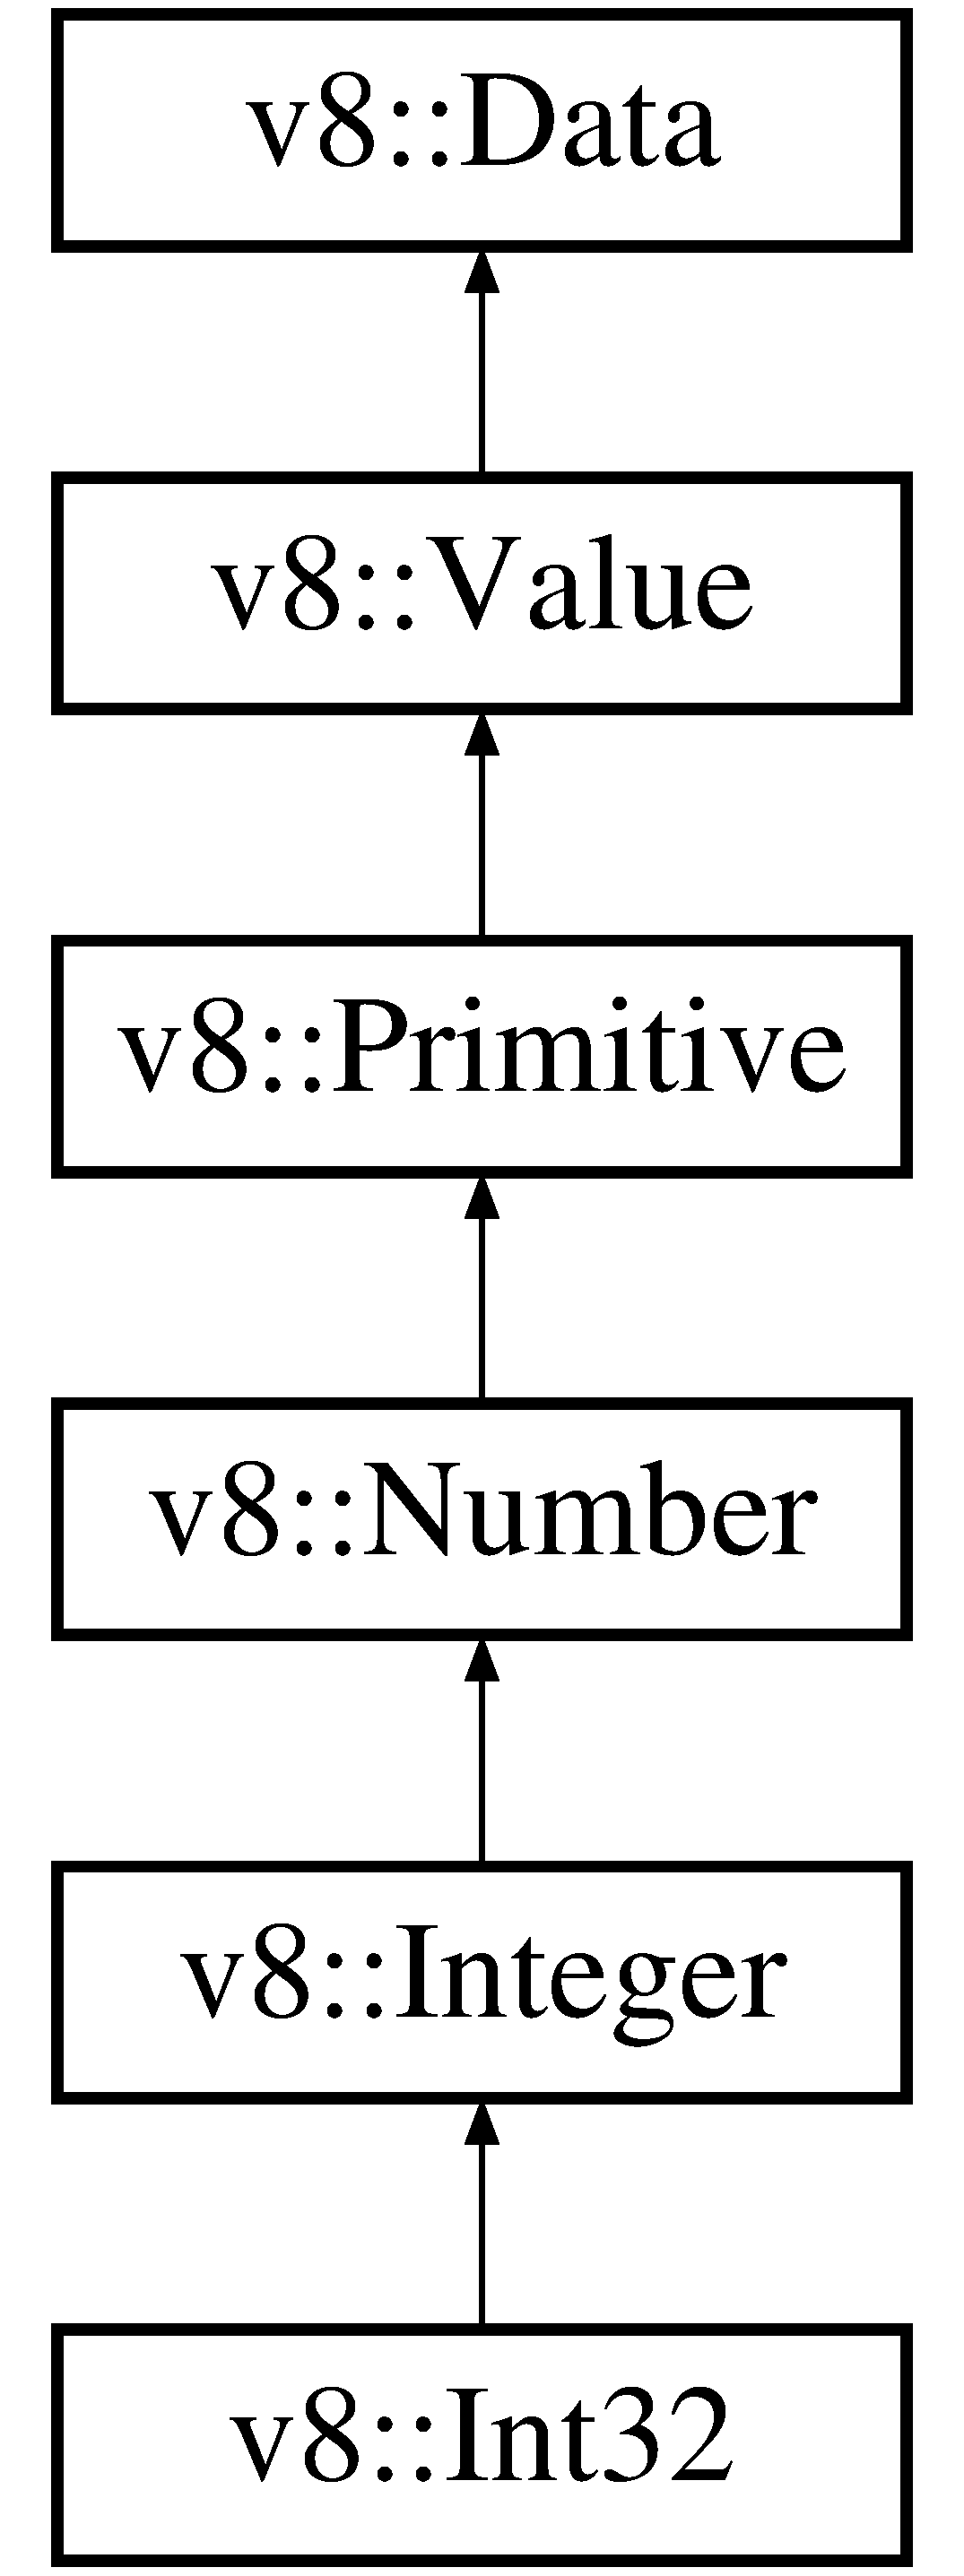
\includegraphics[height=6.000000cm]{classv8_1_1_int32}
\end{center}
\end{figure}
\subsection*{Public Member Functions}
\begin{DoxyCompactItemize}
\item 
\hypertarget{classv8_1_1_int32_a74860c6a524e1fb3f7b685ab0896be4b}{}int32\+\_\+t {\bfseries Value} () const \label{classv8_1_1_int32_a74860c6a524e1fb3f7b685ab0896be4b}

\end{DoxyCompactItemize}
\subsection*{Static Public Member Functions}
\begin{DoxyCompactItemize}
\item 
\hypertarget{classv8_1_1_int32_a910c59c30a7f5f3c96afd0ba10d5339b}{}static V8\+\_\+\+I\+N\+L\+I\+N\+E \hyperlink{classv8_1_1_int32}{Int32} $\ast$ {\bfseries Cast} (\hyperlink{classv8_1_1_value}{v8\+::\+Value} $\ast$obj)\label{classv8_1_1_int32_a910c59c30a7f5f3c96afd0ba10d5339b}

\end{DoxyCompactItemize}


\subsection{Detailed Description}
A Java\+Script value representing a 32-\/bit signed integer. 

The documentation for this class was generated from the following file\+:\begin{DoxyCompactItemize}
\item 
deps/v8/include/v8.\+h\end{DoxyCompactItemize}

\hypertarget{classv8_1_1_integer}{}\section{v8\+:\+:Integer Class Reference}
\label{classv8_1_1_integer}\index{v8\+::\+Integer@{v8\+::\+Integer}}


{\ttfamily \#include $<$v8.\+h$>$}

Inheritance diagram for v8\+:\+:Integer\+:\begin{figure}[H]
\begin{center}
\leavevmode
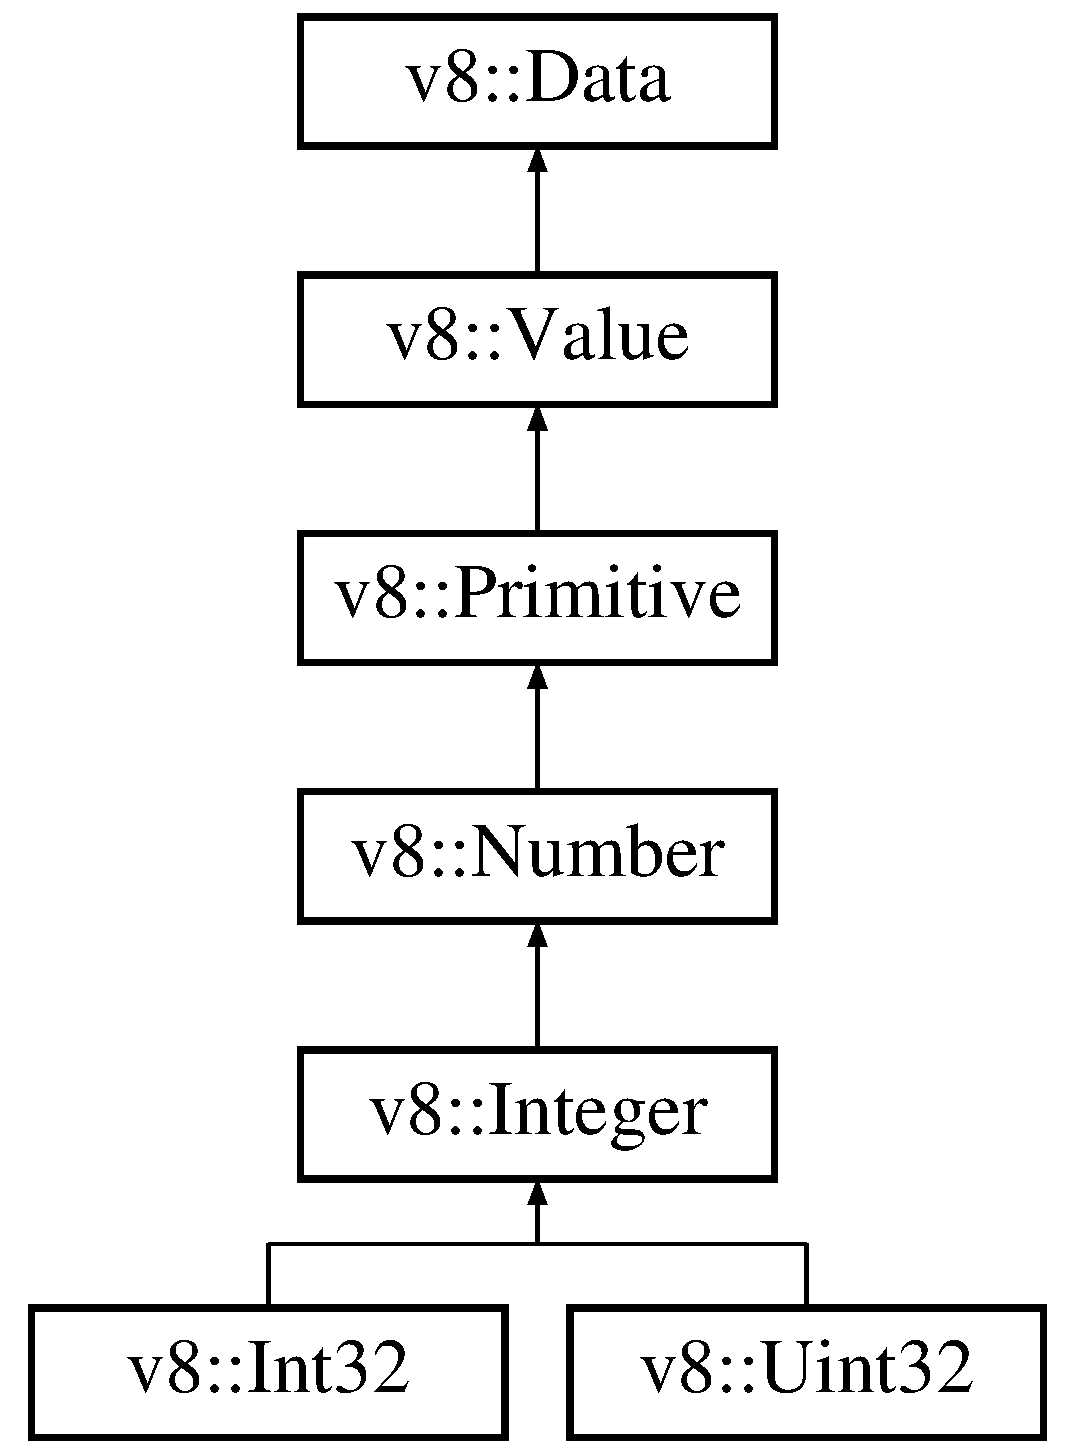
\includegraphics[height=6.000000cm]{classv8_1_1_integer}
\end{center}
\end{figure}
\subsection*{Public Member Functions}
\begin{DoxyCompactItemize}
\item 
\hypertarget{classv8_1_1_integer_ab37942d41df96bf2cd7bb27ba79c4349}{}V8\+E\+X\+P\+O\+R\+T int64\+\_\+t {\bfseries Value} () const \label{classv8_1_1_integer_ab37942d41df96bf2cd7bb27ba79c4349}

\end{DoxyCompactItemize}
\subsection*{Static Public Member Functions}
\begin{DoxyCompactItemize}
\item 
\hypertarget{classv8_1_1_integer_ab715913de664ee8934282de7b3ce4896}{}static V8\+E\+X\+P\+O\+R\+T \hyperlink{classv8_1_1_local}{Local}$<$ \hyperlink{classv8_1_1_integer}{Integer} $>$ {\bfseries New} (int32\+\_\+t value)\label{classv8_1_1_integer_ab715913de664ee8934282de7b3ce4896}

\item 
\hypertarget{classv8_1_1_integer_a5303f8909cf43e495c9524c923d5ffbe}{}static V8\+E\+X\+P\+O\+R\+T \hyperlink{classv8_1_1_local}{Local}$<$ \hyperlink{classv8_1_1_integer}{Integer} $>$ {\bfseries New\+From\+Unsigned} (uint32\+\_\+t value)\label{classv8_1_1_integer_a5303f8909cf43e495c9524c923d5ffbe}

\item 
\hypertarget{classv8_1_1_integer_a9905407109700f9821b31fff6b3d174f}{}static V8\+E\+X\+P\+O\+R\+T \hyperlink{classv8_1_1_local}{Local}$<$ \hyperlink{classv8_1_1_integer}{Integer} $>$ {\bfseries New} (int32\+\_\+t value, \hyperlink{classv8_1_1_isolate}{Isolate} $\ast$)\label{classv8_1_1_integer_a9905407109700f9821b31fff6b3d174f}

\item 
\hypertarget{classv8_1_1_integer_acff93c4ef5ab94d5534ffdf1c7f9ff5d}{}static V8\+E\+X\+P\+O\+R\+T \hyperlink{classv8_1_1_local}{Local}$<$ \hyperlink{classv8_1_1_integer}{Integer} $>$ {\bfseries New\+From\+Unsigned} (uint32\+\_\+t value, \hyperlink{classv8_1_1_isolate}{Isolate} $\ast$)\label{classv8_1_1_integer_acff93c4ef5ab94d5534ffdf1c7f9ff5d}

\item 
\hypertarget{classv8_1_1_integer_a886f73d3d8bb91f8235f66d8dccec12a}{}static \hyperlink{classv8_1_1_integer}{Integer} $\ast$ {\bfseries Cast} (\hyperlink{classv8_1_1_value}{v8\+::\+Value} $\ast$obj)\label{classv8_1_1_integer_a886f73d3d8bb91f8235f66d8dccec12a}

\end{DoxyCompactItemize}


\subsection{Detailed Description}
A Java\+Script value representing a signed integer. 

The documentation for this class was generated from the following file\+:\begin{DoxyCompactItemize}
\item 
deps/v8/include/v8.\+h\end{DoxyCompactItemize}

\hypertarget{structv8_1_1internal_1_1_internal_constants}{}\section{v8\+:\+:internal\+:\+:Internal\+Constants$<$ ptr\+\_\+size $>$ Struct Template Reference}
\label{structv8_1_1internal_1_1_internal_constants}\index{v8\+::internal\+::\+Internal\+Constants$<$ ptr\+\_\+size $>$@{v8\+::internal\+::\+Internal\+Constants$<$ ptr\+\_\+size $>$}}


The documentation for this struct was generated from the following file\+:\begin{DoxyCompactItemize}
\item 
deps/v8/include/v8.\+h\end{DoxyCompactItemize}

\hypertarget{structv8_1_1internal_1_1_internal_constants_3_014_01_4}{}\section{v8\+:\+:internal\+:\+:Internal\+Constants$<$ 4 $>$ Struct Template Reference}
\label{structv8_1_1internal_1_1_internal_constants_3_014_01_4}\index{v8\+::internal\+::\+Internal\+Constants$<$ 4 $>$@{v8\+::internal\+::\+Internal\+Constants$<$ 4 $>$}}
\subsection*{Static Public Attributes}
\begin{DoxyCompactItemize}
\item 
\hypertarget{structv8_1_1internal_1_1_internal_constants_3_014_01_4_a08da692ed2a8b9ec59d9e9a07212bdd3}{}static const int {\bfseries k\+String\+Resource\+Offset} = 3 $\ast$ sizeof(void$\ast$)\label{structv8_1_1internal_1_1_internal_constants_3_014_01_4_a08da692ed2a8b9ec59d9e9a07212bdd3}

\end{DoxyCompactItemize}


The documentation for this struct was generated from the following file\+:\begin{DoxyCompactItemize}
\item 
deps/v8/include/v8.\+h\end{DoxyCompactItemize}

\hypertarget{structv8_1_1internal_1_1_internal_constants_3_018_01_4}{}\section{v8\+:\+:internal\+:\+:Internal\+Constants$<$ 8 $>$ Struct Template Reference}
\label{structv8_1_1internal_1_1_internal_constants_3_018_01_4}\index{v8\+::internal\+::\+Internal\+Constants$<$ 8 $>$@{v8\+::internal\+::\+Internal\+Constants$<$ 8 $>$}}
\subsection*{Static Public Attributes}
\begin{DoxyCompactItemize}
\item 
\hypertarget{structv8_1_1internal_1_1_internal_constants_3_018_01_4_a95faec00d49358d58aafd8cd10257e76}{}static const int {\bfseries k\+String\+Resource\+Offset} = 2 $\ast$ sizeof(void$\ast$)\label{structv8_1_1internal_1_1_internal_constants_3_018_01_4_a95faec00d49358d58aafd8cd10257e76}

\end{DoxyCompactItemize}


The documentation for this struct was generated from the following file\+:\begin{DoxyCompactItemize}
\item 
deps/v8/include/v8.\+h\end{DoxyCompactItemize}

\hypertarget{classv8_1_1internal_1_1_internals}{}\section{v8\+:\+:internal\+:\+:Internals Class Reference}
\label{classv8_1_1internal_1_1_internals}\index{v8\+::internal\+::\+Internals@{v8\+::internal\+::\+Internals}}


{\ttfamily \#include $<$v8.\+h$>$}

\subsection*{Static Public Member Functions}
\begin{DoxyCompactItemize}
\item 
\hypertarget{classv8_1_1internal_1_1_internals_a2d3dc335df00b84e7e242e40012238ae}{}static bool {\bfseries Has\+Heap\+Object\+Tag} (internal\+::\+Object $\ast$value)\label{classv8_1_1internal_1_1_internals_a2d3dc335df00b84e7e242e40012238ae}

\item 
\hypertarget{classv8_1_1internal_1_1_internals_a6163342aeb37f207d618d9fb5d646a04}{}static bool {\bfseries Has\+Smi\+Tag} (internal\+::\+Object $\ast$value)\label{classv8_1_1internal_1_1_internals_a6163342aeb37f207d618d9fb5d646a04}

\item 
\hypertarget{classv8_1_1internal_1_1_internals_a9a26879dad8b7fdd38ebbeaad162b96c}{}static int {\bfseries Smi\+Value} (internal\+::\+Object $\ast$value)\label{classv8_1_1internal_1_1_internals_a9a26879dad8b7fdd38ebbeaad162b96c}

\item 
\hypertarget{classv8_1_1internal_1_1_internals_a072f010fdf69ea2c0d7145190221410f}{}static bool {\bfseries Is\+External\+Two\+Byte\+String} (int instance\+\_\+type)\label{classv8_1_1internal_1_1_internals_a072f010fdf69ea2c0d7145190221410f}

\item 
\hypertarget{classv8_1_1internal_1_1_internals_a457c0c73d5fdf4cc577133edce0ce37b}{}{\footnotesize template$<$typename T $>$ }\\static T {\bfseries Read\+Field} (\hyperlink{classv8_1_1_object}{Object} $\ast$ptr, int offset)\label{classv8_1_1internal_1_1_internals_a457c0c73d5fdf4cc577133edce0ce37b}

\end{DoxyCompactItemize}
\subsection*{Static Public Attributes}
\begin{DoxyCompactItemize}
\item 
\hypertarget{classv8_1_1internal_1_1_internals_a0902a596b5656b4592157eaacc020512}{}static const int {\bfseries k\+Heap\+Object\+Map\+Offset} = 0\label{classv8_1_1internal_1_1_internals_a0902a596b5656b4592157eaacc020512}

\item 
\hypertarget{classv8_1_1internal_1_1_internals_a39ea290dfaa9de300bd79aa73a874a88}{}static const int {\bfseries k\+Map\+Instance\+Type\+Offset} = sizeof(void$\ast$) + sizeof(int)\label{classv8_1_1internal_1_1_internals_a39ea290dfaa9de300bd79aa73a874a88}

\item 
\hypertarget{classv8_1_1internal_1_1_internals_a8c2b35069864f567ca0c571310dd90a1}{}static const int {\bfseries k\+String\+Resource\+Offset} = 2 $\ast$ sizeof(void$\ast$)\label{classv8_1_1internal_1_1_internals_a8c2b35069864f567ca0c571310dd90a1}

\item 
\hypertarget{classv8_1_1internal_1_1_internals_a2f7609ff68b17c9fc15d58bd2dee47aa}{}static const int {\bfseries k\+Proxy\+Proxy\+Offset} = sizeof(void$\ast$)\label{classv8_1_1internal_1_1_internals_a2f7609ff68b17c9fc15d58bd2dee47aa}

\item 
\hypertarget{classv8_1_1internal_1_1_internals_af8faf3ff3271d26bafa6ca0ea87e2a57}{}static const int {\bfseries k\+J\+S\+Object\+Header\+Size} = 3 $\ast$ sizeof(void$\ast$)\label{classv8_1_1internal_1_1_internals_af8faf3ff3271d26bafa6ca0ea87e2a57}

\item 
\hypertarget{classv8_1_1internal_1_1_internals_a5c39a86b30463928ea719def66916507}{}static const int {\bfseries k\+Full\+String\+Representation\+Mask} = 0x07\label{classv8_1_1internal_1_1_internals_a5c39a86b30463928ea719def66916507}

\item 
\hypertarget{classv8_1_1internal_1_1_internals_a73faf917416d2519b65c7255e77a74ce}{}static const int {\bfseries k\+External\+Two\+Byte\+Representation\+Tag} = 0x03\label{classv8_1_1internal_1_1_internals_a73faf917416d2519b65c7255e77a74ce}

\item 
\hypertarget{classv8_1_1internal_1_1_internals_a3a4dd65781f6eee3e625f07e5bbe0c37}{}static const int {\bfseries k\+Aligned\+Pointer\+Shift} = 2\label{classv8_1_1internal_1_1_internals_a3a4dd65781f6eee3e625f07e5bbe0c37}

\item 
\hypertarget{classv8_1_1internal_1_1_internals_ab82a7885d90f825ba1e20defdcb749be}{}static V8\+E\+X\+P\+O\+R\+T int {\bfseries k\+J\+S\+Object\+Type}\label{classv8_1_1internal_1_1_internals_ab82a7885d90f825ba1e20defdcb749be}

\item 
\hypertarget{classv8_1_1internal_1_1_internals_a613844c85afb4e5f1c8a42bbb519d3a1}{}static V8\+E\+X\+P\+O\+R\+T int {\bfseries k\+First\+Nonstring\+Type}\label{classv8_1_1internal_1_1_internals_a613844c85afb4e5f1c8a42bbb519d3a1}

\item 
\hypertarget{classv8_1_1internal_1_1_internals_af263ee9229311eefdc05ad96160e4161}{}static V8\+E\+X\+P\+O\+R\+T int {\bfseries k\+Proxy\+Type}\label{classv8_1_1internal_1_1_internals_af263ee9229311eefdc05ad96160e4161}

\end{DoxyCompactItemize}


\subsection{Detailed Description}
This class exports constants and functionality from within \hyperlink{namespacev8}{v8} that is necessary to implement inline functions in the \hyperlink{namespacev8}{v8} api. Don\textquotesingle{}t depend on functions and constants defined here. 

The documentation for this class was generated from the following file\+:\begin{DoxyCompactItemize}
\item 
deps/v8/include/v8.\+h\end{DoxyCompactItemize}

\hypertarget{classv8_1_1_local}{}\section{v8\+:\+:Local$<$ T $>$ Class Template Reference}
\label{classv8_1_1_local}\index{v8\+::\+Local$<$ T $>$@{v8\+::\+Local$<$ T $>$}}


{\ttfamily \#include $<$v8.\+h$>$}

Inheritance diagram for v8\+:\+:Local$<$ T $>$\+:\begin{figure}[H]
\begin{center}
\leavevmode
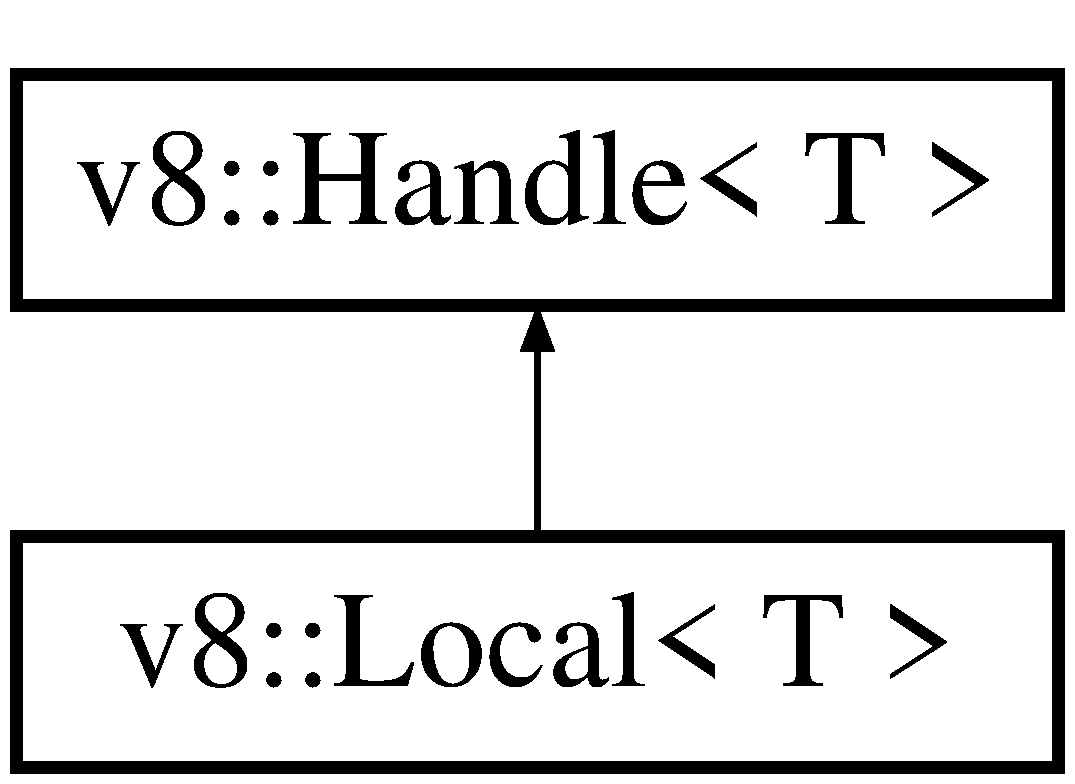
\includegraphics[height=2.000000cm]{classv8_1_1_local}
\end{center}
\end{figure}
\subsection*{Public Member Functions}
\begin{DoxyCompactItemize}
\item 
{\footnotesize template$<$class S $>$ }\\\hyperlink{classv8_1_1_local_af7cf8d2fe7e10a14ad382189712adaff}{Local} (\hyperlink{classv8_1_1_local}{Local}$<$ S $>$ that)
\item 
\hypertarget{classv8_1_1_local_aaa90419a2288a960d4a139ff226914b2}{}{\footnotesize template$<$class S $>$ }\\{\bfseries Local} (S $\ast$that)\label{classv8_1_1_local_aaa90419a2288a960d4a139ff226914b2}

\item 
\hypertarget{classv8_1_1_local_afd7f49264bab1faf07eee38beb6d5a0f}{}{\footnotesize template$<$class S $>$ }\\\hyperlink{classv8_1_1_local}{Local}$<$ S $>$ {\bfseries As} ()\label{classv8_1_1_local_afd7f49264bab1faf07eee38beb6d5a0f}

\end{DoxyCompactItemize}
\subsection*{Static Public Member Functions}
\begin{DoxyCompactItemize}
\item 
\hypertarget{classv8_1_1_local_a8e76791c0614ec0feed0e5a3a9d6e9f8}{}{\footnotesize template$<$class S $>$ }\\static \hyperlink{classv8_1_1_local}{Local}$<$ T $>$ {\bfseries Cast} (\hyperlink{classv8_1_1_local}{Local}$<$ S $>$ that)\label{classv8_1_1_local_a8e76791c0614ec0feed0e5a3a9d6e9f8}

\item 
static \hyperlink{classv8_1_1_local}{Local}$<$ T $>$ \hyperlink{classv8_1_1_local_ac4024a7e2aea140c6aaa38fc32d5a840}{New} (\hyperlink{classv8_1_1_handle}{Handle}$<$ T $>$ that)
\end{DoxyCompactItemize}


\subsection{Detailed Description}
\subsubsection*{template$<$class T$>$class v8\+::\+Local$<$ T $>$}

A light-\/weight stack-\/allocated object handle. All operations that return objects from within \hyperlink{namespacev8}{v8} return them in local handles. They are created within Handle\+Scopes, and all local handles allocated within a handle scope are destroyed when the handle scope is destroyed. Hence it is not necessary to explicitly deallocate local handles. 

\subsection{Constructor \& Destructor Documentation}
\hypertarget{classv8_1_1_local_af7cf8d2fe7e10a14ad382189712adaff}{}\index{v8\+::\+Local@{v8\+::\+Local}!Local@{Local}}
\index{Local@{Local}!v8\+::\+Local@{v8\+::\+Local}}
\subsubsection[{Local}]{\setlength{\rightskip}{0pt plus 5cm}template$<$class T$>$ template$<$class S $>$ {\bf v8\+::\+Local}$<$ T $>$\+::{\bf Local} (
\begin{DoxyParamCaption}
\item[{{\bf Local}$<$ S $>$}]{that}
\end{DoxyParamCaption}
)\hspace{0.3cm}{\ttfamily [inline]}}\label{classv8_1_1_local_af7cf8d2fe7e10a14ad382189712adaff}
This check fails when trying to convert between incompatible handles. For example, converting from a Handle$<$\+String$>$ to a Handle$<$\+Number$>$.

\subsection{Member Function Documentation}
\hypertarget{classv8_1_1_local_ac4024a7e2aea140c6aaa38fc32d5a840}{}\index{v8\+::\+Local@{v8\+::\+Local}!New@{New}}
\index{New@{New}!v8\+::\+Local@{v8\+::\+Local}}
\subsubsection[{New}]{\setlength{\rightskip}{0pt plus 5cm}template$<$class T $>$ {\bf Local}$<$ T $>$ {\bf v8\+::\+Local}$<$ T $>$\+::New (
\begin{DoxyParamCaption}
\item[{{\bf Handle}$<$ T $>$}]{that}
\end{DoxyParamCaption}
)\hspace{0.3cm}{\ttfamily [inline]}, {\ttfamily [static]}}\label{classv8_1_1_local_ac4024a7e2aea140c6aaa38fc32d5a840}
Create a local handle for the content of another handle. The referee is kept alive by the local handle even when the original handle is destroyed/disposed. 

The documentation for this class was generated from the following file\+:\begin{DoxyCompactItemize}
\item 
deps/v8/include/v8.\+h\end{DoxyCompactItemize}

\hypertarget{classv8_1_1_locker}{}\section{v8\+:\+:Locker Class Reference}
\label{classv8_1_1_locker}\index{v8\+::\+Locker@{v8\+::\+Locker}}
\subsection*{Public Member Functions}
\begin{DoxyCompactItemize}
\item 
\hyperlink{classv8_1_1_locker_a84728a02fbc178d9d3be2a169af45bbb}{Locker} (\hyperlink{classv8_1_1_isolate}{Isolate} $\ast$isolate=N\+U\+L\+L)
\end{DoxyCompactItemize}
\subsection*{Static Public Member Functions}
\begin{DoxyCompactItemize}
\item 
static void \hyperlink{classv8_1_1_locker_a272bf054bb4d8bb51b0101ba7bf3456f}{Start\+Preemption} (int every\+\_\+n\+\_\+ms)
\item 
static void \hyperlink{classv8_1_1_locker_ab79915454872612692808fea64f539ec}{Stop\+Preemption} ()
\item 
static bool \hyperlink{classv8_1_1_locker_acc59b0b99564f25529d6fbcf2536094c}{Is\+Locked} (\hyperlink{classv8_1_1_isolate}{Isolate} $\ast$isolate=N\+U\+L\+L)
\item 
static bool \hyperlink{classv8_1_1_locker_a19d2b640f2f9b3dd0ec3a6c09a0442ed}{Is\+Active} ()
\end{DoxyCompactItemize}


\subsection{Constructor \& Destructor Documentation}
\hypertarget{classv8_1_1_locker_a84728a02fbc178d9d3be2a169af45bbb}{}\index{v8\+::\+Locker@{v8\+::\+Locker}!Locker@{Locker}}
\index{Locker@{Locker}!v8\+::\+Locker@{v8\+::\+Locker}}
\subsubsection[{Locker}]{\setlength{\rightskip}{0pt plus 5cm}v8\+::\+Locker\+::\+Locker (
\begin{DoxyParamCaption}
\item[{{\bf Isolate} $\ast$}]{isolate = {\ttfamily NULL}}
\end{DoxyParamCaption}
)\hspace{0.3cm}{\ttfamily [explicit]}}\label{classv8_1_1_locker_a84728a02fbc178d9d3be2a169af45bbb}
Initialize \hyperlink{classv8_1_1_locker}{Locker} for a given \hyperlink{classv8_1_1_isolate}{Isolate}. N\+U\+L\+L means default isolate. 

\subsection{Member Function Documentation}
\hypertarget{classv8_1_1_locker_a19d2b640f2f9b3dd0ec3a6c09a0442ed}{}\index{v8\+::\+Locker@{v8\+::\+Locker}!Is\+Active@{Is\+Active}}
\index{Is\+Active@{Is\+Active}!v8\+::\+Locker@{v8\+::\+Locker}}
\subsubsection[{Is\+Active}]{\setlength{\rightskip}{0pt plus 5cm}static bool v8\+::\+Locker\+::\+Is\+Active (
\begin{DoxyParamCaption}
{}
\end{DoxyParamCaption}
)\hspace{0.3cm}{\ttfamily [static]}}\label{classv8_1_1_locker_a19d2b640f2f9b3dd0ec3a6c09a0442ed}
Returns whether \hyperlink{classv8_1_1_locker}{v8\+::\+Locker} is being used by this \hyperlink{classv8_1_1_v8}{V8} instance. \hypertarget{classv8_1_1_locker_acc59b0b99564f25529d6fbcf2536094c}{}\index{v8\+::\+Locker@{v8\+::\+Locker}!Is\+Locked@{Is\+Locked}}
\index{Is\+Locked@{Is\+Locked}!v8\+::\+Locker@{v8\+::\+Locker}}
\subsubsection[{Is\+Locked}]{\setlength{\rightskip}{0pt plus 5cm}static bool v8\+::\+Locker\+::\+Is\+Locked (
\begin{DoxyParamCaption}
\item[{{\bf Isolate} $\ast$}]{isolate = {\ttfamily NULL}}
\end{DoxyParamCaption}
)\hspace{0.3cm}{\ttfamily [static]}}\label{classv8_1_1_locker_acc59b0b99564f25529d6fbcf2536094c}
Returns whether or not the locker for a given isolate, or default isolate if N\+U\+L\+L is given, is locked by the current thread. \hypertarget{classv8_1_1_locker_a272bf054bb4d8bb51b0101ba7bf3456f}{}\index{v8\+::\+Locker@{v8\+::\+Locker}!Start\+Preemption@{Start\+Preemption}}
\index{Start\+Preemption@{Start\+Preemption}!v8\+::\+Locker@{v8\+::\+Locker}}
\subsubsection[{Start\+Preemption}]{\setlength{\rightskip}{0pt plus 5cm}static void v8\+::\+Locker\+::\+Start\+Preemption (
\begin{DoxyParamCaption}
\item[{int}]{every\+\_\+n\+\_\+ms}
\end{DoxyParamCaption}
)\hspace{0.3cm}{\ttfamily [static]}}\label{classv8_1_1_locker_a272bf054bb4d8bb51b0101ba7bf3456f}
Start preemption.

When preemption is started, a timer is fired every n milliseconds that will switch between multiple threads that are in contention for the \hyperlink{classv8_1_1_v8}{V8} lock. \hypertarget{classv8_1_1_locker_ab79915454872612692808fea64f539ec}{}\index{v8\+::\+Locker@{v8\+::\+Locker}!Stop\+Preemption@{Stop\+Preemption}}
\index{Stop\+Preemption@{Stop\+Preemption}!v8\+::\+Locker@{v8\+::\+Locker}}
\subsubsection[{Stop\+Preemption}]{\setlength{\rightskip}{0pt plus 5cm}static void v8\+::\+Locker\+::\+Stop\+Preemption (
\begin{DoxyParamCaption}
{}
\end{DoxyParamCaption}
)\hspace{0.3cm}{\ttfamily [static]}}\label{classv8_1_1_locker_ab79915454872612692808fea64f539ec}
Stop preemption. 

The documentation for this class was generated from the following file\+:\begin{DoxyCompactItemize}
\item 
deps/v8/include/v8.\+h\end{DoxyCompactItemize}

\hypertarget{classv8_1_1_message}{}\section{v8\+:\+:Message Class Reference}
\label{classv8_1_1_message}\index{v8\+::\+Message@{v8\+::\+Message}}


{\ttfamily \#include $<$v8.\+h$>$}

\subsection*{Public Member Functions}
\begin{DoxyCompactItemize}
\item 
\hypertarget{classv8_1_1_message_a72f26c7b684bbfbd14d5970849fdf3d2}{}\hyperlink{classv8_1_1_local}{Local}$<$ \hyperlink{classv8_1_1_string}{String} $>$ {\bfseries Get} () const \label{classv8_1_1_message_a72f26c7b684bbfbd14d5970849fdf3d2}

\item 
\hypertarget{classv8_1_1_message_a0d5cceb5128a147818c72b82950e475d}{}\hyperlink{classv8_1_1_local}{Local}$<$ \hyperlink{classv8_1_1_string}{String} $>$ {\bfseries Get\+Source\+Line} () const \label{classv8_1_1_message_a0d5cceb5128a147818c72b82950e475d}

\item 
\hyperlink{classv8_1_1_script_origin}{Script\+Origin} \hyperlink{classv8_1_1_message_ae0fc442f44bd2b600c4d89a50cf3abd9}{Get\+Script\+Origin} () const 
\item 
\hyperlink{classv8_1_1_handle}{Handle}$<$ \hyperlink{classv8_1_1_value}{Value} $>$ \hyperlink{classv8_1_1_message_ac5d31afb758897cd1653c5eb3327a4d6}{Get\+Script\+Resource\+Name} () const 
\item 
\hyperlink{classv8_1_1_handle}{Handle}$<$ \hyperlink{classv8_1_1_stack_trace}{Stack\+Trace} $>$ \hyperlink{classv8_1_1_message_adeffa297a5a28955dd16c084632aa645}{Get\+Stack\+Trace} () const 
\item 
int \hyperlink{classv8_1_1_message_a67f97fd76b8f98ed65743b9615d64a79}{Get\+Line\+Number} () const 
\item 
int \hyperlink{classv8_1_1_message_a31a550a1d3d09a2d72d0742be821956f}{Get\+Start\+Position} () const 
\item 
int \hyperlink{classv8_1_1_message_a50cbec87379e628b1647466926882037}{Get\+End\+Position} () const 
\item 
int \hyperlink{classv8_1_1_message_aab8007ba81d3f195280bce0693810cc2}{Get\+Start\+Column} () const 
\item 
int \hyperlink{classv8_1_1_message_aaf82cd7f7449add5f50d4253499cad05}{Get\+End\+Column} () const 
\item 
bool \hyperlink{classv8_1_1_message_a03228f50c40c45da52f424bdd64598d1}{Is\+Shared\+Cross\+Origin} () const 
\end{DoxyCompactItemize}
\subsection*{Static Public Member Functions}
\begin{DoxyCompactItemize}
\item 
\hypertarget{classv8_1_1_message_ae5d67d123c5611e6bc36824c938cbfa5}{}static void {\bfseries Print\+Current\+Stack\+Trace} (\hyperlink{classv8_1_1_isolate}{Isolate} $\ast$isolate, F\+I\+L\+E $\ast$out)\label{classv8_1_1_message_ae5d67d123c5611e6bc36824c938cbfa5}

\end{DoxyCompactItemize}
\subsection*{Static Public Attributes}
\begin{DoxyCompactItemize}
\item 
\hypertarget{classv8_1_1_message_a35649a6c0c813ba82c9886a2b17da124}{}static const int {\bfseries k\+No\+Line\+Number\+Info} = 0\label{classv8_1_1_message_a35649a6c0c813ba82c9886a2b17da124}

\item 
\hypertarget{classv8_1_1_message_a8cb643dbf408b0fd2526b23a8202c4a6}{}static const int {\bfseries k\+No\+Column\+Info} = 0\label{classv8_1_1_message_a8cb643dbf408b0fd2526b23a8202c4a6}

\item 
\hypertarget{classv8_1_1_message_a5aac643173466e88544cb1daa74553d6}{}static const int {\bfseries k\+No\+Script\+Id\+Info} = 0\label{classv8_1_1_message_a5aac643173466e88544cb1daa74553d6}

\end{DoxyCompactItemize}


\subsection{Detailed Description}
An error message. 

\subsection{Member Function Documentation}
\hypertarget{classv8_1_1_message_aaf82cd7f7449add5f50d4253499cad05}{}\index{v8\+::\+Message@{v8\+::\+Message}!Get\+End\+Column@{Get\+End\+Column}}
\index{Get\+End\+Column@{Get\+End\+Column}!v8\+::\+Message@{v8\+::\+Message}}
\subsubsection[{Get\+End\+Column}]{\setlength{\rightskip}{0pt plus 5cm}int v8\+::\+Message\+::\+Get\+End\+Column (
\begin{DoxyParamCaption}
{}
\end{DoxyParamCaption}
) const}\label{classv8_1_1_message_aaf82cd7f7449add5f50d4253499cad05}
Returns the index within the line of the last character where the error occurred. \hypertarget{classv8_1_1_message_a50cbec87379e628b1647466926882037}{}\index{v8\+::\+Message@{v8\+::\+Message}!Get\+End\+Position@{Get\+End\+Position}}
\index{Get\+End\+Position@{Get\+End\+Position}!v8\+::\+Message@{v8\+::\+Message}}
\subsubsection[{Get\+End\+Position}]{\setlength{\rightskip}{0pt plus 5cm}int v8\+::\+Message\+::\+Get\+End\+Position (
\begin{DoxyParamCaption}
{}
\end{DoxyParamCaption}
) const}\label{classv8_1_1_message_a50cbec87379e628b1647466926882037}
Returns the index within the script of the last character where the error occurred. \hypertarget{classv8_1_1_message_a67f97fd76b8f98ed65743b9615d64a79}{}\index{v8\+::\+Message@{v8\+::\+Message}!Get\+Line\+Number@{Get\+Line\+Number}}
\index{Get\+Line\+Number@{Get\+Line\+Number}!v8\+::\+Message@{v8\+::\+Message}}
\subsubsection[{Get\+Line\+Number}]{\setlength{\rightskip}{0pt plus 5cm}int v8\+::\+Message\+::\+Get\+Line\+Number (
\begin{DoxyParamCaption}
{}
\end{DoxyParamCaption}
) const}\label{classv8_1_1_message_a67f97fd76b8f98ed65743b9615d64a79}
Returns the number, 1-\/based, of the line where the error occurred. \hypertarget{classv8_1_1_message_ae0fc442f44bd2b600c4d89a50cf3abd9}{}\index{v8\+::\+Message@{v8\+::\+Message}!Get\+Script\+Origin@{Get\+Script\+Origin}}
\index{Get\+Script\+Origin@{Get\+Script\+Origin}!v8\+::\+Message@{v8\+::\+Message}}
\subsubsection[{Get\+Script\+Origin}]{\setlength{\rightskip}{0pt plus 5cm}{\bf Script\+Origin} v8\+::\+Message\+::\+Get\+Script\+Origin (
\begin{DoxyParamCaption}
{}
\end{DoxyParamCaption}
) const}\label{classv8_1_1_message_ae0fc442f44bd2b600c4d89a50cf3abd9}
Returns the origin for the script from where the function causing the error originates. \hypertarget{classv8_1_1_message_ac5d31afb758897cd1653c5eb3327a4d6}{}\index{v8\+::\+Message@{v8\+::\+Message}!Get\+Script\+Resource\+Name@{Get\+Script\+Resource\+Name}}
\index{Get\+Script\+Resource\+Name@{Get\+Script\+Resource\+Name}!v8\+::\+Message@{v8\+::\+Message}}
\subsubsection[{Get\+Script\+Resource\+Name}]{\setlength{\rightskip}{0pt plus 5cm}{\bf Handle}$<${\bf Value}$>$ v8\+::\+Message\+::\+Get\+Script\+Resource\+Name (
\begin{DoxyParamCaption}
{}
\end{DoxyParamCaption}
) const}\label{classv8_1_1_message_ac5d31afb758897cd1653c5eb3327a4d6}
Returns the resource name for the script from where the function causing the error originates. \hypertarget{classv8_1_1_message_adeffa297a5a28955dd16c084632aa645}{}\index{v8\+::\+Message@{v8\+::\+Message}!Get\+Stack\+Trace@{Get\+Stack\+Trace}}
\index{Get\+Stack\+Trace@{Get\+Stack\+Trace}!v8\+::\+Message@{v8\+::\+Message}}
\subsubsection[{Get\+Stack\+Trace}]{\setlength{\rightskip}{0pt plus 5cm}{\bf Handle}$<${\bf Stack\+Trace}$>$ v8\+::\+Message\+::\+Get\+Stack\+Trace (
\begin{DoxyParamCaption}
{}
\end{DoxyParamCaption}
) const}\label{classv8_1_1_message_adeffa297a5a28955dd16c084632aa645}
\hyperlink{classv8_1_1_exception}{Exception} stack trace. By default stack traces are not captured for uncaught exceptions. Set\+Capture\+Stack\+Trace\+For\+Uncaught\+Exceptions allows to change this option. \hypertarget{classv8_1_1_message_aab8007ba81d3f195280bce0693810cc2}{}\index{v8\+::\+Message@{v8\+::\+Message}!Get\+Start\+Column@{Get\+Start\+Column}}
\index{Get\+Start\+Column@{Get\+Start\+Column}!v8\+::\+Message@{v8\+::\+Message}}
\subsubsection[{Get\+Start\+Column}]{\setlength{\rightskip}{0pt plus 5cm}int v8\+::\+Message\+::\+Get\+Start\+Column (
\begin{DoxyParamCaption}
{}
\end{DoxyParamCaption}
) const}\label{classv8_1_1_message_aab8007ba81d3f195280bce0693810cc2}
Returns the index within the line of the first character where the error occurred. \hypertarget{classv8_1_1_message_a31a550a1d3d09a2d72d0742be821956f}{}\index{v8\+::\+Message@{v8\+::\+Message}!Get\+Start\+Position@{Get\+Start\+Position}}
\index{Get\+Start\+Position@{Get\+Start\+Position}!v8\+::\+Message@{v8\+::\+Message}}
\subsubsection[{Get\+Start\+Position}]{\setlength{\rightskip}{0pt plus 5cm}int v8\+::\+Message\+::\+Get\+Start\+Position (
\begin{DoxyParamCaption}
{}
\end{DoxyParamCaption}
) const}\label{classv8_1_1_message_a31a550a1d3d09a2d72d0742be821956f}
Returns the index within the script of the first character where the error occurred. \hypertarget{classv8_1_1_message_a03228f50c40c45da52f424bdd64598d1}{}\index{v8\+::\+Message@{v8\+::\+Message}!Is\+Shared\+Cross\+Origin@{Is\+Shared\+Cross\+Origin}}
\index{Is\+Shared\+Cross\+Origin@{Is\+Shared\+Cross\+Origin}!v8\+::\+Message@{v8\+::\+Message}}
\subsubsection[{Is\+Shared\+Cross\+Origin}]{\setlength{\rightskip}{0pt plus 5cm}bool v8\+::\+Message\+::\+Is\+Shared\+Cross\+Origin (
\begin{DoxyParamCaption}
{}
\end{DoxyParamCaption}
) const}\label{classv8_1_1_message_a03228f50c40c45da52f424bdd64598d1}
Passes on the value set by the embedder when it fed the script from which this \hyperlink{classv8_1_1_message}{Message} was generated to \hyperlink{classv8_1_1_v8}{V8}. 

The documentation for this class was generated from the following file\+:\begin{DoxyCompactItemize}
\item 
deps/v8/include/v8.\+h\end{DoxyCompactItemize}

\hypertarget{classv8_1_1_debug_1_1_message}{}\section{v8\+:\+:Debug\+:\+:Message Class Reference}
\label{classv8_1_1_debug_1_1_message}\index{v8\+::\+Debug\+::\+Message@{v8\+::\+Debug\+::\+Message}}


{\ttfamily \#include $<$v8-\/debug.\+h$>$}

\subsection*{Public Member Functions}
\begin{DoxyCompactItemize}
\item 
virtual bool \hyperlink{classv8_1_1_debug_1_1_message_a36ade83a9c960ce581b1a4051f763785}{Is\+Event} () const =0
\item 
\hypertarget{classv8_1_1_debug_1_1_message_a1d65d6efbb5adb96406f7e285bb25ee3}{}virtual bool {\bfseries Is\+Response} () const =0\label{classv8_1_1_debug_1_1_message_a1d65d6efbb5adb96406f7e285bb25ee3}

\item 
\hypertarget{classv8_1_1_debug_1_1_message_a8a99a5c9fe0db14fbaccaed297d9c203}{}virtual Debug\+Event {\bfseries Get\+Event} () const =0\label{classv8_1_1_debug_1_1_message_a8a99a5c9fe0db14fbaccaed297d9c203}

\item 
virtual bool \hyperlink{classv8_1_1_debug_1_1_message_af8d236b6a334423732a38cbf8cfd7aef}{Will\+Start\+Running} () const =0
\item 
virtual \hyperlink{classv8_1_1_handle}{Handle}$<$ \hyperlink{classv8_1_1_object}{Object} $>$ \hyperlink{classv8_1_1_debug_1_1_message_aa54e11b06d304e8b8f34cc79ee49d869}{Get\+Execution\+State} () const =0
\item 
\hypertarget{classv8_1_1_debug_1_1_message_aa18f6c01d91d176d4e3d0a018890e59a}{}virtual \hyperlink{classv8_1_1_handle}{Handle}$<$ \hyperlink{classv8_1_1_object}{Object} $>$ {\bfseries Get\+Event\+Data} () const =0\label{classv8_1_1_debug_1_1_message_aa18f6c01d91d176d4e3d0a018890e59a}

\item 
virtual \hyperlink{classv8_1_1_handle}{Handle}$<$ \hyperlink{classv8_1_1_string}{String} $>$ \hyperlink{classv8_1_1_debug_1_1_message_a41076f64f82c927cbb2fe5c8325557d5}{Get\+J\+S\+O\+N} () const =0
\item 
virtual \hyperlink{classv8_1_1_handle}{Handle}$<$ \hyperlink{classv8_1_1_context}{Context} $>$ \hyperlink{classv8_1_1_debug_1_1_message_a34ff90d879888746a7a0eacebd6aa088}{Get\+Event\+Context} () const =0
\item 
virtual \hyperlink{classv8_1_1_debug_1_1_client_data}{Client\+Data} $\ast$ \hyperlink{classv8_1_1_debug_1_1_message_ab81bb81d233f5f37e6626a7bcac22142}{Get\+Client\+Data} () const =0
\end{DoxyCompactItemize}


\subsection{Detailed Description}
A message object passed to the debug message handler. 

\subsection{Member Function Documentation}
\hypertarget{classv8_1_1_debug_1_1_message_ab81bb81d233f5f37e6626a7bcac22142}{}\index{v8\+::\+Debug\+::\+Message@{v8\+::\+Debug\+::\+Message}!Get\+Client\+Data@{Get\+Client\+Data}}
\index{Get\+Client\+Data@{Get\+Client\+Data}!v8\+::\+Debug\+::\+Message@{v8\+::\+Debug\+::\+Message}}
\subsubsection[{Get\+Client\+Data}]{\setlength{\rightskip}{0pt plus 5cm}virtual {\bf Client\+Data}$\ast$ v8\+::\+Debug\+::\+Message\+::\+Get\+Client\+Data (
\begin{DoxyParamCaption}
{}
\end{DoxyParamCaption}
) const\hspace{0.3cm}{\ttfamily [pure virtual]}}\label{classv8_1_1_debug_1_1_message_ab81bb81d233f5f37e6626a7bcac22142}
Client data passed with the corresponding request if any. This is the client\+\_\+data data value passed into Debug\+::\+Send\+Command along with the request that led to the message or N\+U\+L\+L if the message is an event. The debugger takes ownership of the data and will delete it even if there is no message handler. \hypertarget{classv8_1_1_debug_1_1_message_a34ff90d879888746a7a0eacebd6aa088}{}\index{v8\+::\+Debug\+::\+Message@{v8\+::\+Debug\+::\+Message}!Get\+Event\+Context@{Get\+Event\+Context}}
\index{Get\+Event\+Context@{Get\+Event\+Context}!v8\+::\+Debug\+::\+Message@{v8\+::\+Debug\+::\+Message}}
\subsubsection[{Get\+Event\+Context}]{\setlength{\rightskip}{0pt plus 5cm}virtual {\bf Handle}$<${\bf Context}$>$ v8\+::\+Debug\+::\+Message\+::\+Get\+Event\+Context (
\begin{DoxyParamCaption}
{}
\end{DoxyParamCaption}
) const\hspace{0.3cm}{\ttfamily [pure virtual]}}\label{classv8_1_1_debug_1_1_message_a34ff90d879888746a7a0eacebd6aa088}
Get the context active when the debug event happened. Note this is not the current active context as the Java\+Script part of the debugger is running in its own context which is entered at this point. \hypertarget{classv8_1_1_debug_1_1_message_aa54e11b06d304e8b8f34cc79ee49d869}{}\index{v8\+::\+Debug\+::\+Message@{v8\+::\+Debug\+::\+Message}!Get\+Execution\+State@{Get\+Execution\+State}}
\index{Get\+Execution\+State@{Get\+Execution\+State}!v8\+::\+Debug\+::\+Message@{v8\+::\+Debug\+::\+Message}}
\subsubsection[{Get\+Execution\+State}]{\setlength{\rightskip}{0pt plus 5cm}virtual {\bf Handle}$<${\bf Object}$>$ v8\+::\+Debug\+::\+Message\+::\+Get\+Execution\+State (
\begin{DoxyParamCaption}
{}
\end{DoxyParamCaption}
) const\hspace{0.3cm}{\ttfamily [pure virtual]}}\label{classv8_1_1_debug_1_1_message_aa54e11b06d304e8b8f34cc79ee49d869}
Access to execution state and event data. Don\textquotesingle{}t store these cross callbacks as their content becomes invalid. These objects are from the debugger event that started the debug message loop. \hypertarget{classv8_1_1_debug_1_1_message_a41076f64f82c927cbb2fe5c8325557d5}{}\index{v8\+::\+Debug\+::\+Message@{v8\+::\+Debug\+::\+Message}!Get\+J\+S\+O\+N@{Get\+J\+S\+O\+N}}
\index{Get\+J\+S\+O\+N@{Get\+J\+S\+O\+N}!v8\+::\+Debug\+::\+Message@{v8\+::\+Debug\+::\+Message}}
\subsubsection[{Get\+J\+S\+O\+N}]{\setlength{\rightskip}{0pt plus 5cm}virtual {\bf Handle}$<${\bf String}$>$ v8\+::\+Debug\+::\+Message\+::\+Get\+J\+S\+O\+N (
\begin{DoxyParamCaption}
{}
\end{DoxyParamCaption}
) const\hspace{0.3cm}{\ttfamily [pure virtual]}}\label{classv8_1_1_debug_1_1_message_a41076f64f82c927cbb2fe5c8325557d5}
Get the debugger protocol J\+S\+O\+N. \hypertarget{classv8_1_1_debug_1_1_message_a36ade83a9c960ce581b1a4051f763785}{}\index{v8\+::\+Debug\+::\+Message@{v8\+::\+Debug\+::\+Message}!Is\+Event@{Is\+Event}}
\index{Is\+Event@{Is\+Event}!v8\+::\+Debug\+::\+Message@{v8\+::\+Debug\+::\+Message}}
\subsubsection[{Is\+Event}]{\setlength{\rightskip}{0pt plus 5cm}virtual bool v8\+::\+Debug\+::\+Message\+::\+Is\+Event (
\begin{DoxyParamCaption}
{}
\end{DoxyParamCaption}
) const\hspace{0.3cm}{\ttfamily [pure virtual]}}\label{classv8_1_1_debug_1_1_message_a36ade83a9c960ce581b1a4051f763785}
Check type of message. \hypertarget{classv8_1_1_debug_1_1_message_af8d236b6a334423732a38cbf8cfd7aef}{}\index{v8\+::\+Debug\+::\+Message@{v8\+::\+Debug\+::\+Message}!Will\+Start\+Running@{Will\+Start\+Running}}
\index{Will\+Start\+Running@{Will\+Start\+Running}!v8\+::\+Debug\+::\+Message@{v8\+::\+Debug\+::\+Message}}
\subsubsection[{Will\+Start\+Running}]{\setlength{\rightskip}{0pt plus 5cm}virtual bool v8\+::\+Debug\+::\+Message\+::\+Will\+Start\+Running (
\begin{DoxyParamCaption}
{}
\end{DoxyParamCaption}
) const\hspace{0.3cm}{\ttfamily [pure virtual]}}\label{classv8_1_1_debug_1_1_message_af8d236b6a334423732a38cbf8cfd7aef}
Indicate whether this is a response to a continue command which will start the V\+M running after this is processed. 

The documentation for this class was generated from the following file\+:\begin{DoxyCompactItemize}
\item 
deps/v8/include/v8-\/debug.\+h\end{DoxyCompactItemize}

\hypertarget{classv8_1_1_number}{}\section{v8\+:\+:Number Class Reference}
\label{classv8_1_1_number}\index{v8\+::\+Number@{v8\+::\+Number}}


{\ttfamily \#include $<$v8.\+h$>$}

Inheritance diagram for v8\+:\+:Number\+:\begin{figure}[H]
\begin{center}
\leavevmode
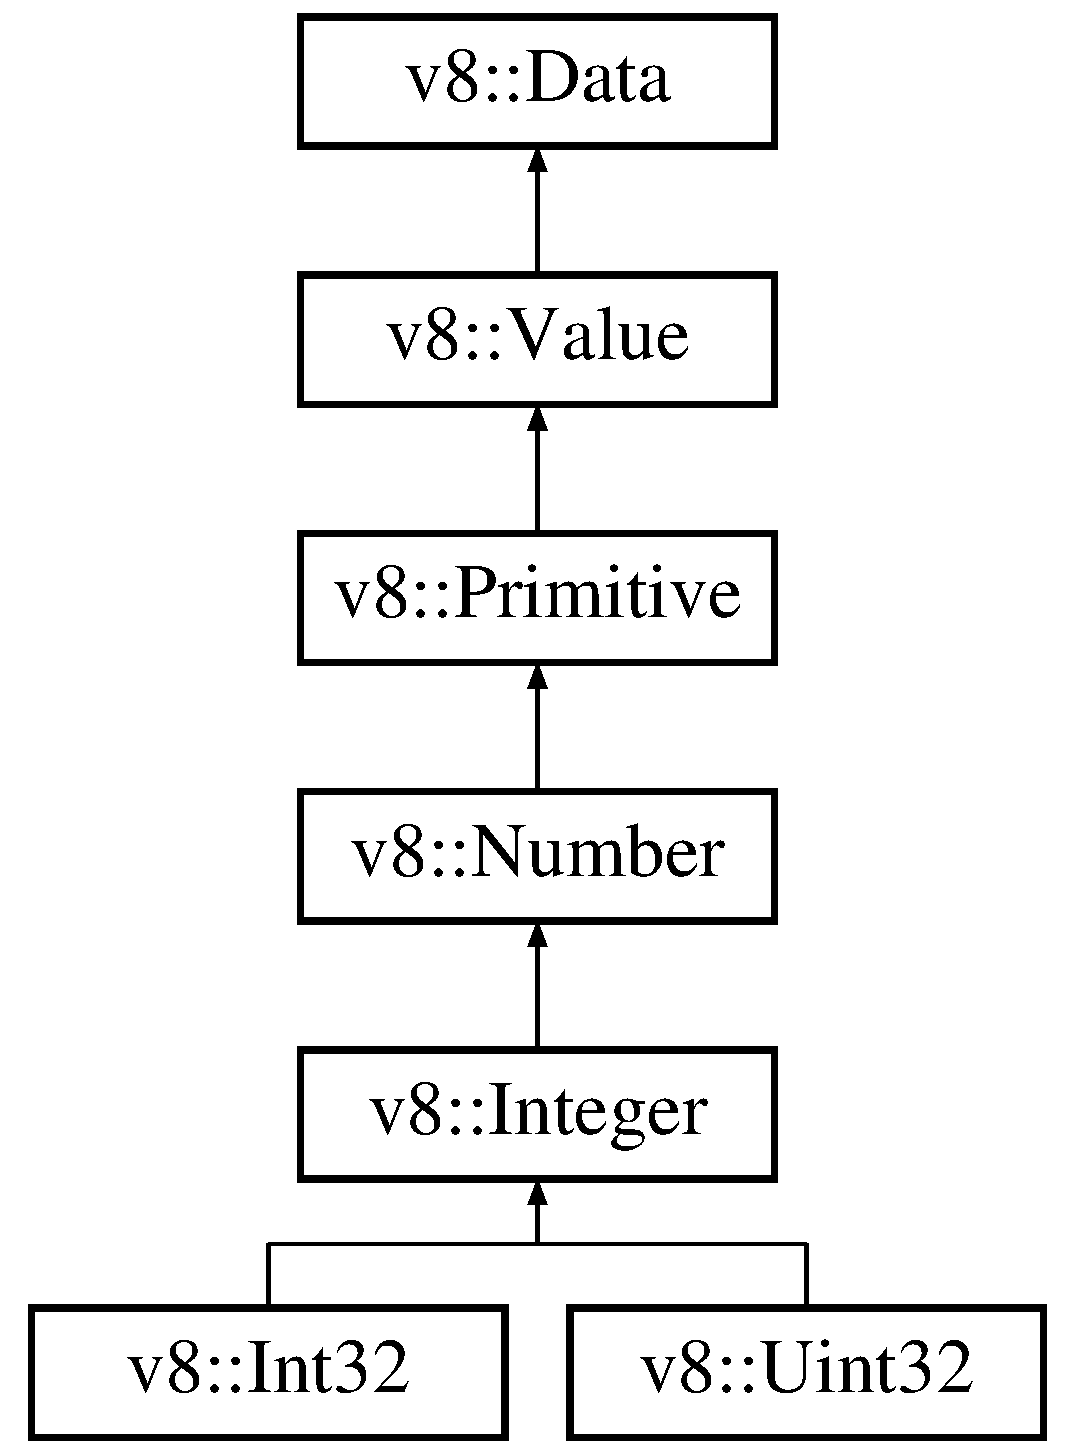
\includegraphics[height=6.000000cm]{classv8_1_1_number}
\end{center}
\end{figure}
\subsection*{Public Member Functions}
\begin{DoxyCompactItemize}
\item 
\hypertarget{classv8_1_1_number_a98717c8d0e7731e2ba57d2ccfbe62697}{}V8\+E\+X\+P\+O\+R\+T double {\bfseries Value} () const \label{classv8_1_1_number_a98717c8d0e7731e2ba57d2ccfbe62697}

\end{DoxyCompactItemize}
\subsection*{Static Public Member Functions}
\begin{DoxyCompactItemize}
\item 
\hypertarget{classv8_1_1_number_a527a9e071536ca2cf57ce2eabea0bf36}{}static V8\+E\+X\+P\+O\+R\+T \hyperlink{classv8_1_1_local}{Local}$<$ \hyperlink{classv8_1_1_number}{Number} $>$ {\bfseries New} (double value)\label{classv8_1_1_number_a527a9e071536ca2cf57ce2eabea0bf36}

\item 
\hypertarget{classv8_1_1_number_a053d48e0003104308963a4a7e3881912}{}static \hyperlink{classv8_1_1_number}{Number} $\ast$ {\bfseries Cast} (\hyperlink{classv8_1_1_value}{v8\+::\+Value} $\ast$obj)\label{classv8_1_1_number_a053d48e0003104308963a4a7e3881912}

\end{DoxyCompactItemize}


\subsection{Detailed Description}
A Java\+Script number value (E\+C\+M\+A-\/262, 4.\+3.\+20) 

The documentation for this class was generated from the following file\+:\begin{DoxyCompactItemize}
\item 
deps/v8/include/v8.\+h\end{DoxyCompactItemize}

\hypertarget{classv8_1_1_object}{}\section{v8\+:\+:Object Class Reference}
\label{classv8_1_1_object}\index{v8\+::\+Object@{v8\+::\+Object}}


{\ttfamily \#include $<$v8.\+h$>$}

Inheritance diagram for v8\+:\+:Object\+:\begin{figure}[H]
\begin{center}
\leavevmode
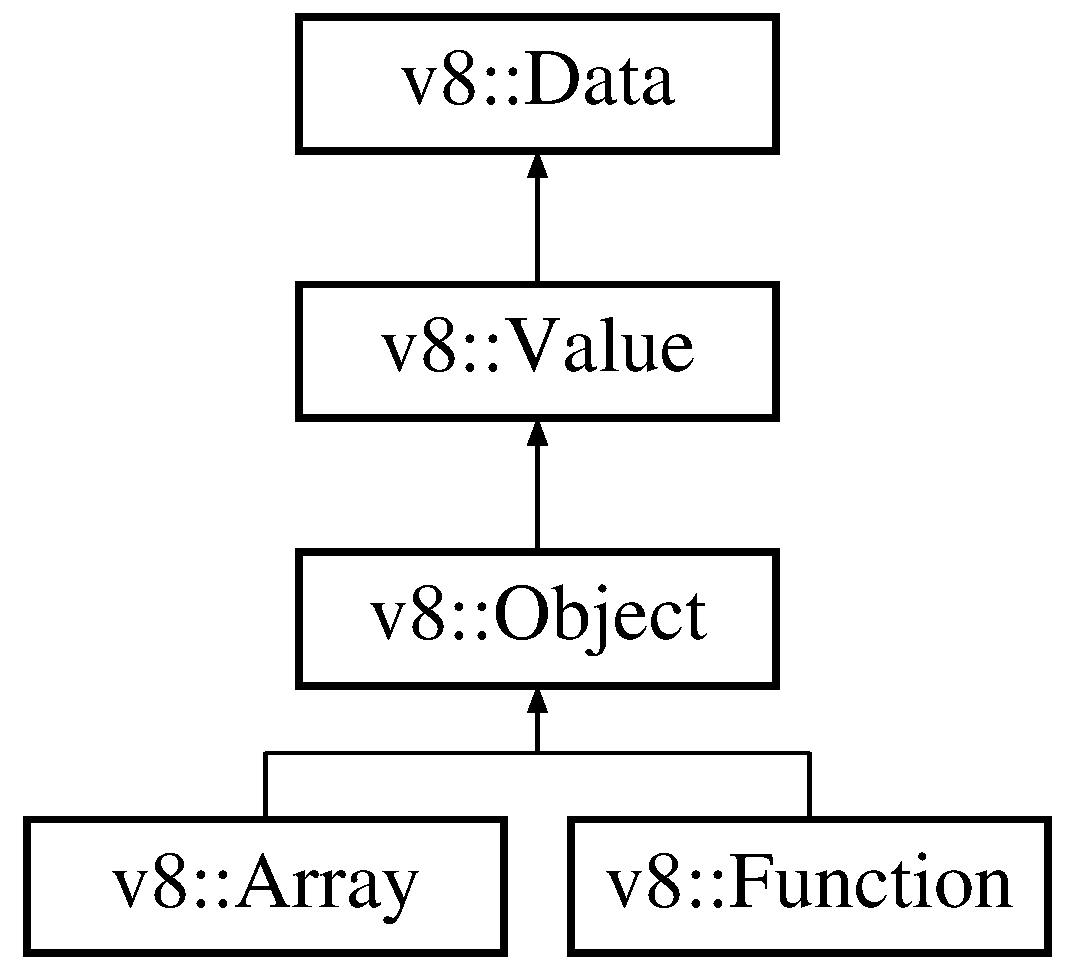
\includegraphics[height=4.000000cm]{classv8_1_1_object}
\end{center}
\end{figure}
\subsection*{Public Member Functions}
\begin{DoxyCompactItemize}
\item 
\hypertarget{classv8_1_1_object_a208583edae8e8da2c083879429ee3184}{}bool {\bfseries Set} (\hyperlink{classv8_1_1_handle}{Handle}$<$ \hyperlink{classv8_1_1_value}{Value} $>$ key, \hyperlink{classv8_1_1_handle}{Handle}$<$ \hyperlink{classv8_1_1_value}{Value} $>$ value, Property\+Attribute attribs=None)\label{classv8_1_1_object_a208583edae8e8da2c083879429ee3184}

\item 
\hypertarget{classv8_1_1_object_aa89f3dce24a3a3431295218d24498c52}{}bool {\bfseries Force\+Set} (\hyperlink{classv8_1_1_handle}{Handle}$<$ \hyperlink{classv8_1_1_value}{Value} $>$ key, \hyperlink{classv8_1_1_handle}{Handle}$<$ \hyperlink{classv8_1_1_value}{Value} $>$ value, Property\+Attribute attribs=None)\label{classv8_1_1_object_aa89f3dce24a3a3431295218d24498c52}

\item 
\hypertarget{classv8_1_1_object_a976f0329ff7465c124652d633d469c06}{}\hyperlink{classv8_1_1_local}{Local}$<$ \hyperlink{classv8_1_1_value}{Value} $>$ {\bfseries Get} (\hyperlink{classv8_1_1_handle}{Handle}$<$ \hyperlink{classv8_1_1_value}{Value} $>$ key)\label{classv8_1_1_object_a976f0329ff7465c124652d633d469c06}

\item 
\hypertarget{classv8_1_1_object_a5ae86b3538e5afbca528a0e3bdd896cc}{}bool {\bfseries Has} (\hyperlink{classv8_1_1_handle}{Handle}$<$ \hyperlink{classv8_1_1_string}{String} $>$ key)\label{classv8_1_1_object_a5ae86b3538e5afbca528a0e3bdd896cc}

\item 
\hypertarget{classv8_1_1_object_a51d85c48448af7812f60c1ca75111dd8}{}bool {\bfseries Delete} (\hyperlink{classv8_1_1_handle}{Handle}$<$ \hyperlink{classv8_1_1_string}{String} $>$ key)\label{classv8_1_1_object_a51d85c48448af7812f60c1ca75111dd8}

\item 
\hypertarget{classv8_1_1_object_a8e7f3b8b70eb17bcb5cc087d5b6746d6}{}bool {\bfseries Force\+Delete} (\hyperlink{classv8_1_1_handle}{Handle}$<$ \hyperlink{classv8_1_1_value}{Value} $>$ key)\label{classv8_1_1_object_a8e7f3b8b70eb17bcb5cc087d5b6746d6}

\item 
\hypertarget{classv8_1_1_object_ac547af2f2d256d96991ff20159a44bfd}{}bool {\bfseries Has} (uint32\+\_\+t index)\label{classv8_1_1_object_ac547af2f2d256d96991ff20159a44bfd}

\item 
\hypertarget{classv8_1_1_object_a63f88a22cb5d994eedc1efc79520bc42}{}bool {\bfseries Delete} (uint32\+\_\+t index)\label{classv8_1_1_object_a63f88a22cb5d994eedc1efc79520bc42}

\item 
\hyperlink{classv8_1_1_local}{Local}$<$ \hyperlink{classv8_1_1_array}{Array} $>$ \hyperlink{classv8_1_1_object_a9f45786246c6e6027b32f685d900a41f}{Get\+Property\+Names} ()
\item 
\hyperlink{classv8_1_1_local}{Local}$<$ \hyperlink{classv8_1_1_value}{Value} $>$ \hyperlink{classv8_1_1_object_ae8d3fed7d6dbd667c29cabb3039fe7af}{Get\+Prototype} ()
\item 
\hyperlink{classv8_1_1_local}{Local}$<$ \hyperlink{classv8_1_1_object}{Object} $>$ \hyperlink{classv8_1_1_object_ab2c5f7369abf08ae8f44dc84f5aa335a}{Find\+Instance\+In\+Prototype\+Chain} (\hyperlink{classv8_1_1_handle}{Handle}$<$ \hyperlink{classv8_1_1_function_template}{Function\+Template} $>$ tmpl)
\item 
\hyperlink{classv8_1_1_local}{Local}$<$ \hyperlink{classv8_1_1_string}{String} $>$ \hyperlink{classv8_1_1_object_aeb2f524c806075e5f9032a24afd86869}{Object\+Proto\+To\+String} ()
\item 
int \hyperlink{classv8_1_1_object_aaec28576353eebe6fee113bce2718ecc}{Internal\+Field\+Count} ()
\item 
\hyperlink{classv8_1_1_local}{Local}$<$ \hyperlink{classv8_1_1_value}{Value} $>$ \hyperlink{classv8_1_1_object_aa3324fdf652d8ac3b2f27faa0559231d}{Get\+Internal\+Field} (int index)
\item 
void \hyperlink{classv8_1_1_object_a361b1781e7db29b17b063ef31315989e}{Set\+Internal\+Field} (int index, \hyperlink{classv8_1_1_handle}{Handle}$<$ \hyperlink{classv8_1_1_value}{Value} $>$ value)
\item 
void $\ast$ \hyperlink{classv8_1_1_object_a8ef1f3e0d4f4cecc54d5e0248bc45694}{Get\+Pointer\+From\+Internal\+Field} (int index)
\item 
void \hyperlink{classv8_1_1_object_a697c8b6945ab4cb4bf468414bb4c1234}{Set\+Pointer\+In\+Internal\+Field} (int index, void $\ast$value)
\item 
\hypertarget{classv8_1_1_object_a5c29998a9ec60802b052f528a1aaa7fd}{}bool {\bfseries Has\+Real\+Named\+Property} (\hyperlink{classv8_1_1_handle}{Handle}$<$ \hyperlink{classv8_1_1_string}{String} $>$ key)\label{classv8_1_1_object_a5c29998a9ec60802b052f528a1aaa7fd}

\item 
\hypertarget{classv8_1_1_object_a29dce0e7da968dae54614501f035f7e9}{}bool {\bfseries Has\+Real\+Indexed\+Property} (uint32\+\_\+t index)\label{classv8_1_1_object_a29dce0e7da968dae54614501f035f7e9}

\item 
\hypertarget{classv8_1_1_object_aa501acb241c3b3a941b9f48c23b1e1cd}{}bool {\bfseries Has\+Real\+Named\+Callback\+Property} (\hyperlink{classv8_1_1_handle}{Handle}$<$ \hyperlink{classv8_1_1_string}{String} $>$ key)\label{classv8_1_1_object_aa501acb241c3b3a941b9f48c23b1e1cd}

\item 
\hyperlink{classv8_1_1_handle}{Handle}$<$ \hyperlink{classv8_1_1_value}{Value} $>$ \hyperlink{classv8_1_1_object_abcede2bb76c86c5071314ffb340cf68c}{Get\+Real\+Named\+Property\+In\+Prototype\+Chain} (\hyperlink{classv8_1_1_handle}{Handle}$<$ \hyperlink{classv8_1_1_string}{String} $>$ key)
\item 
bool \hyperlink{classv8_1_1_object_a1e96fcb9ee17101c0299ec68f2cf8610}{Has\+Named\+Lookup\+Interceptor} ()
\item 
bool \hyperlink{classv8_1_1_object_a278913bcd203434870ce5184a538a9af}{Has\+Indexed\+Lookup\+Interceptor} ()
\item 
void \hyperlink{classv8_1_1_object_a6e9fe342c0f77995defa6b479d01a3bd}{Turn\+On\+Access\+Check} ()
\item 
int \hyperlink{classv8_1_1_object_ac1ece41e81a499920ec3a2a3471653bc}{Get\+Identity\+Hash} ()
\item 
bool \hyperlink{classv8_1_1_object_a2200482b09feb914dc91d8256671f7f0}{Set\+Hidden\+Value} (\hyperlink{classv8_1_1_handle}{Handle}$<$ \hyperlink{classv8_1_1_string}{String} $>$ key, \hyperlink{classv8_1_1_handle}{Handle}$<$ \hyperlink{classv8_1_1_value}{Value} $>$ value)
\item 
\hypertarget{classv8_1_1_object_a0fb148558e1749b04a2e13b2c9fa4441}{}\hyperlink{classv8_1_1_local}{Local}$<$ \hyperlink{classv8_1_1_value}{Value} $>$ {\bfseries Get\+Hidden\+Value} (\hyperlink{classv8_1_1_handle}{Handle}$<$ \hyperlink{classv8_1_1_string}{String} $>$ key)\label{classv8_1_1_object_a0fb148558e1749b04a2e13b2c9fa4441}

\item 
\hypertarget{classv8_1_1_object_ab1d274da1949b1f68087728760ee4172}{}bool {\bfseries Delete\+Hidden\+Value} (\hyperlink{classv8_1_1_handle}{Handle}$<$ \hyperlink{classv8_1_1_string}{String} $>$ key)\label{classv8_1_1_object_ab1d274da1949b1f68087728760ee4172}

\item 
bool \hyperlink{classv8_1_1_object_a3c1f8cfb754b5d29d5f1998b2047befd}{Is\+Dirty} ()
\item 
\hyperlink{classv8_1_1_local}{Local}$<$ \hyperlink{classv8_1_1_object}{Object} $>$ \hyperlink{classv8_1_1_object_a5018c9d085aa71f65530cf1e073a04ad}{Clone} ()
\item 
void \hyperlink{classv8_1_1_object_a6c552c4817b9a0eff1fb12b7ef089026}{Set\+Indexed\+Properties\+To\+Pixel\+Data} (uint8\+\_\+t $\ast$data, int length)
\end{DoxyCompactItemize}
\subsection*{Static Public Member Functions}
\begin{DoxyCompactItemize}
\item 
\hypertarget{classv8_1_1_object_a4360445f2166250431502b82242ba873}{}static \hyperlink{classv8_1_1_local}{Local}$<$ \hyperlink{classv8_1_1_object}{Object} $>$ {\bfseries New} ()\label{classv8_1_1_object_a4360445f2166250431502b82242ba873}

\item 
\hypertarget{classv8_1_1_object_a1f9ac46d0b164197318ce81dc0ec1343}{}static \hyperlink{classv8_1_1_object}{Object} $\ast$ {\bfseries Cast} (\hyperlink{classv8_1_1_value}{Value} $\ast$obj)\label{classv8_1_1_object_a1f9ac46d0b164197318ce81dc0ec1343}

\end{DoxyCompactItemize}


\subsection{Detailed Description}
A Java\+Script object (E\+C\+M\+A-\/262, 4.\+3.\+3) 

\subsection{Member Function Documentation}
\hypertarget{classv8_1_1_object_a5018c9d085aa71f65530cf1e073a04ad}{}\index{v8\+::\+Object@{v8\+::\+Object}!Clone@{Clone}}
\index{Clone@{Clone}!v8\+::\+Object@{v8\+::\+Object}}
\subsubsection[{Clone}]{\setlength{\rightskip}{0pt plus 5cm}{\bf Local}$<${\bf Object}$>$ v8\+::\+Object\+::\+Clone (
\begin{DoxyParamCaption}
{}
\end{DoxyParamCaption}
)}\label{classv8_1_1_object_a5018c9d085aa71f65530cf1e073a04ad}
Clone this object with a fast but shallow copy. Values will point to the same values as the original object. \hypertarget{classv8_1_1_object_ab2c5f7369abf08ae8f44dc84f5aa335a}{}\index{v8\+::\+Object@{v8\+::\+Object}!Find\+Instance\+In\+Prototype\+Chain@{Find\+Instance\+In\+Prototype\+Chain}}
\index{Find\+Instance\+In\+Prototype\+Chain@{Find\+Instance\+In\+Prototype\+Chain}!v8\+::\+Object@{v8\+::\+Object}}
\subsubsection[{Find\+Instance\+In\+Prototype\+Chain}]{\setlength{\rightskip}{0pt plus 5cm}{\bf Local}$<${\bf Object}$>$ v8\+::\+Object\+::\+Find\+Instance\+In\+Prototype\+Chain (
\begin{DoxyParamCaption}
\item[{{\bf Handle}$<$ {\bf Function\+Template} $>$}]{tmpl}
\end{DoxyParamCaption}
)}\label{classv8_1_1_object_ab2c5f7369abf08ae8f44dc84f5aa335a}
Finds an instance of the given function template in the prototype chain. \hypertarget{classv8_1_1_object_ac1ece41e81a499920ec3a2a3471653bc}{}\index{v8\+::\+Object@{v8\+::\+Object}!Get\+Identity\+Hash@{Get\+Identity\+Hash}}
\index{Get\+Identity\+Hash@{Get\+Identity\+Hash}!v8\+::\+Object@{v8\+::\+Object}}
\subsubsection[{Get\+Identity\+Hash}]{\setlength{\rightskip}{0pt plus 5cm}int v8\+::\+Object\+::\+Get\+Identity\+Hash (
\begin{DoxyParamCaption}
{}
\end{DoxyParamCaption}
)}\label{classv8_1_1_object_ac1ece41e81a499920ec3a2a3471653bc}
Returns the identity hash for this object. The current implemenation uses a hidden property on the object to store the identity hash.

The return value will never be 0. Also, it is not guaranteed to be unique. \hypertarget{classv8_1_1_object_aa3324fdf652d8ac3b2f27faa0559231d}{}\index{v8\+::\+Object@{v8\+::\+Object}!Get\+Internal\+Field@{Get\+Internal\+Field}}
\index{Get\+Internal\+Field@{Get\+Internal\+Field}!v8\+::\+Object@{v8\+::\+Object}}
\subsubsection[{Get\+Internal\+Field}]{\setlength{\rightskip}{0pt plus 5cm}{\bf Local}$<$ {\bf Value} $>$ v8\+::\+Object\+::\+Get\+Internal\+Field (
\begin{DoxyParamCaption}
\item[{int}]{index}
\end{DoxyParamCaption}
)\hspace{0.3cm}{\ttfamily [inline]}}\label{classv8_1_1_object_aa3324fdf652d8ac3b2f27faa0559231d}
Gets the value in an internal field. \hypertarget{classv8_1_1_object_a8ef1f3e0d4f4cecc54d5e0248bc45694}{}\index{v8\+::\+Object@{v8\+::\+Object}!Get\+Pointer\+From\+Internal\+Field@{Get\+Pointer\+From\+Internal\+Field}}
\index{Get\+Pointer\+From\+Internal\+Field@{Get\+Pointer\+From\+Internal\+Field}!v8\+::\+Object@{v8\+::\+Object}}
\subsubsection[{Get\+Pointer\+From\+Internal\+Field}]{\setlength{\rightskip}{0pt plus 5cm}void $\ast$ v8\+::\+Object\+::\+Get\+Pointer\+From\+Internal\+Field (
\begin{DoxyParamCaption}
\item[{int}]{index}
\end{DoxyParamCaption}
)\hspace{0.3cm}{\ttfamily [inline]}}\label{classv8_1_1_object_a8ef1f3e0d4f4cecc54d5e0248bc45694}
Gets a native pointer from an internal field. \hypertarget{classv8_1_1_object_a9f45786246c6e6027b32f685d900a41f}{}\index{v8\+::\+Object@{v8\+::\+Object}!Get\+Property\+Names@{Get\+Property\+Names}}
\index{Get\+Property\+Names@{Get\+Property\+Names}!v8\+::\+Object@{v8\+::\+Object}}
\subsubsection[{Get\+Property\+Names}]{\setlength{\rightskip}{0pt plus 5cm}{\bf Local}$<${\bf Array}$>$ v8\+::\+Object\+::\+Get\+Property\+Names (
\begin{DoxyParamCaption}
{}
\end{DoxyParamCaption}
)}\label{classv8_1_1_object_a9f45786246c6e6027b32f685d900a41f}
Returns an array containing the names of the enumerable properties of this object, including properties from prototype objects. The array returned by this method contains the same values as would be enumerated by a for-\/in statement over this object. \hypertarget{classv8_1_1_object_ae8d3fed7d6dbd667c29cabb3039fe7af}{}\index{v8\+::\+Object@{v8\+::\+Object}!Get\+Prototype@{Get\+Prototype}}
\index{Get\+Prototype@{Get\+Prototype}!v8\+::\+Object@{v8\+::\+Object}}
\subsubsection[{Get\+Prototype}]{\setlength{\rightskip}{0pt plus 5cm}{\bf Local}$<${\bf Value}$>$ v8\+::\+Object\+::\+Get\+Prototype (
\begin{DoxyParamCaption}
{}
\end{DoxyParamCaption}
)}\label{classv8_1_1_object_ae8d3fed7d6dbd667c29cabb3039fe7af}
Get the prototype object. This does not skip objects marked to be skipped by {\bfseries proto} and it does not consult the security handler. \hypertarget{classv8_1_1_object_abcede2bb76c86c5071314ffb340cf68c}{}\index{v8\+::\+Object@{v8\+::\+Object}!Get\+Real\+Named\+Property\+In\+Prototype\+Chain@{Get\+Real\+Named\+Property\+In\+Prototype\+Chain}}
\index{Get\+Real\+Named\+Property\+In\+Prototype\+Chain@{Get\+Real\+Named\+Property\+In\+Prototype\+Chain}!v8\+::\+Object@{v8\+::\+Object}}
\subsubsection[{Get\+Real\+Named\+Property\+In\+Prototype\+Chain}]{\setlength{\rightskip}{0pt plus 5cm}{\bf Handle}$<${\bf Value}$>$ v8\+::\+Object\+::\+Get\+Real\+Named\+Property\+In\+Prototype\+Chain (
\begin{DoxyParamCaption}
\item[{{\bf Handle}$<$ {\bf String} $>$}]{key}
\end{DoxyParamCaption}
)}\label{classv8_1_1_object_abcede2bb76c86c5071314ffb340cf68c}
If result.\+Is\+Empty() no real property was located in the prototype chain. This means interceptors in the prototype chain are not called. \hypertarget{classv8_1_1_object_a278913bcd203434870ce5184a538a9af}{}\index{v8\+::\+Object@{v8\+::\+Object}!Has\+Indexed\+Lookup\+Interceptor@{Has\+Indexed\+Lookup\+Interceptor}}
\index{Has\+Indexed\+Lookup\+Interceptor@{Has\+Indexed\+Lookup\+Interceptor}!v8\+::\+Object@{v8\+::\+Object}}
\subsubsection[{Has\+Indexed\+Lookup\+Interceptor}]{\setlength{\rightskip}{0pt plus 5cm}bool v8\+::\+Object\+::\+Has\+Indexed\+Lookup\+Interceptor (
\begin{DoxyParamCaption}
{}
\end{DoxyParamCaption}
)}\label{classv8_1_1_object_a278913bcd203434870ce5184a538a9af}
Tests for an index lookup interceptor. \hypertarget{classv8_1_1_object_a1e96fcb9ee17101c0299ec68f2cf8610}{}\index{v8\+::\+Object@{v8\+::\+Object}!Has\+Named\+Lookup\+Interceptor@{Has\+Named\+Lookup\+Interceptor}}
\index{Has\+Named\+Lookup\+Interceptor@{Has\+Named\+Lookup\+Interceptor}!v8\+::\+Object@{v8\+::\+Object}}
\subsubsection[{Has\+Named\+Lookup\+Interceptor}]{\setlength{\rightskip}{0pt plus 5cm}bool v8\+::\+Object\+::\+Has\+Named\+Lookup\+Interceptor (
\begin{DoxyParamCaption}
{}
\end{DoxyParamCaption}
)}\label{classv8_1_1_object_a1e96fcb9ee17101c0299ec68f2cf8610}
Tests for a named lookup interceptor. \hypertarget{classv8_1_1_object_aaec28576353eebe6fee113bce2718ecc}{}\index{v8\+::\+Object@{v8\+::\+Object}!Internal\+Field\+Count@{Internal\+Field\+Count}}
\index{Internal\+Field\+Count@{Internal\+Field\+Count}!v8\+::\+Object@{v8\+::\+Object}}
\subsubsection[{Internal\+Field\+Count}]{\setlength{\rightskip}{0pt plus 5cm}int v8\+::\+Object\+::\+Internal\+Field\+Count (
\begin{DoxyParamCaption}
{}
\end{DoxyParamCaption}
)}\label{classv8_1_1_object_aaec28576353eebe6fee113bce2718ecc}
Gets the number of internal fields for this \hyperlink{classv8_1_1_object}{Object}. \hypertarget{classv8_1_1_object_a3c1f8cfb754b5d29d5f1998b2047befd}{}\index{v8\+::\+Object@{v8\+::\+Object}!Is\+Dirty@{Is\+Dirty}}
\index{Is\+Dirty@{Is\+Dirty}!v8\+::\+Object@{v8\+::\+Object}}
\subsubsection[{Is\+Dirty}]{\setlength{\rightskip}{0pt plus 5cm}bool v8\+::\+Object\+::\+Is\+Dirty (
\begin{DoxyParamCaption}
{}
\end{DoxyParamCaption}
)}\label{classv8_1_1_object_a3c1f8cfb754b5d29d5f1998b2047befd}
Returns true if this is an instance of an api function (one created from a function created from a function template) and has been modified since it was created. Note that this method is conservative and may return true for objects that haven\textquotesingle{}t actually been modified. \hypertarget{classv8_1_1_object_aeb2f524c806075e5f9032a24afd86869}{}\index{v8\+::\+Object@{v8\+::\+Object}!Object\+Proto\+To\+String@{Object\+Proto\+To\+String}}
\index{Object\+Proto\+To\+String@{Object\+Proto\+To\+String}!v8\+::\+Object@{v8\+::\+Object}}
\subsubsection[{Object\+Proto\+To\+String}]{\setlength{\rightskip}{0pt plus 5cm}{\bf Local}$<${\bf String}$>$ v8\+::\+Object\+::\+Object\+Proto\+To\+String (
\begin{DoxyParamCaption}
{}
\end{DoxyParamCaption}
)}\label{classv8_1_1_object_aeb2f524c806075e5f9032a24afd86869}
Call builtin Object.\+prototype.\+to\+String on this object. This is different from Value\+::\+To\+String() that may call user-\/defined to\+String function. This one does not. \hypertarget{classv8_1_1_object_a2200482b09feb914dc91d8256671f7f0}{}\index{v8\+::\+Object@{v8\+::\+Object}!Set\+Hidden\+Value@{Set\+Hidden\+Value}}
\index{Set\+Hidden\+Value@{Set\+Hidden\+Value}!v8\+::\+Object@{v8\+::\+Object}}
\subsubsection[{Set\+Hidden\+Value}]{\setlength{\rightskip}{0pt plus 5cm}bool v8\+::\+Object\+::\+Set\+Hidden\+Value (
\begin{DoxyParamCaption}
\item[{{\bf Handle}$<$ {\bf String} $>$}]{key, }
\item[{{\bf Handle}$<$ {\bf Value} $>$}]{value}
\end{DoxyParamCaption}
)}\label{classv8_1_1_object_a2200482b09feb914dc91d8256671f7f0}
Access hidden properties on Java\+Script objects. These properties are hidden from the executing Java\+Script and only accessible through the \hyperlink{classv8_1_1_v8}{V8} C++ A\+P\+I. Hidden properties introduced by \hyperlink{classv8_1_1_v8}{V8} internally (for example the identity hash) are prefixed with \char`\"{}v8\+::\char`\"{}. \hypertarget{classv8_1_1_object_a6c552c4817b9a0eff1fb12b7ef089026}{}\index{v8\+::\+Object@{v8\+::\+Object}!Set\+Indexed\+Properties\+To\+Pixel\+Data@{Set\+Indexed\+Properties\+To\+Pixel\+Data}}
\index{Set\+Indexed\+Properties\+To\+Pixel\+Data@{Set\+Indexed\+Properties\+To\+Pixel\+Data}!v8\+::\+Object@{v8\+::\+Object}}
\subsubsection[{Set\+Indexed\+Properties\+To\+Pixel\+Data}]{\setlength{\rightskip}{0pt plus 5cm}void v8\+::\+Object\+::\+Set\+Indexed\+Properties\+To\+Pixel\+Data (
\begin{DoxyParamCaption}
\item[{uint8\+\_\+t $\ast$}]{data, }
\item[{int}]{length}
\end{DoxyParamCaption}
)}\label{classv8_1_1_object_a6c552c4817b9a0eff1fb12b7ef089026}
Set the backing store of the indexed properties to be managed by the embedding layer. Access to the indexed properties will follow the rules spelled out in Canvas\+Pixel\+Array. Note\+: The embedding program still owns the data and needs to ensure that the backing store is preserved while \hyperlink{classv8_1_1_v8}{V8} has a reference. \hypertarget{classv8_1_1_object_a361b1781e7db29b17b063ef31315989e}{}\index{v8\+::\+Object@{v8\+::\+Object}!Set\+Internal\+Field@{Set\+Internal\+Field}}
\index{Set\+Internal\+Field@{Set\+Internal\+Field}!v8\+::\+Object@{v8\+::\+Object}}
\subsubsection[{Set\+Internal\+Field}]{\setlength{\rightskip}{0pt plus 5cm}void v8\+::\+Object\+::\+Set\+Internal\+Field (
\begin{DoxyParamCaption}
\item[{int}]{index, }
\item[{{\bf Handle}$<$ {\bf Value} $>$}]{value}
\end{DoxyParamCaption}
)}\label{classv8_1_1_object_a361b1781e7db29b17b063ef31315989e}
Sets the value in an internal field. \hypertarget{classv8_1_1_object_a697c8b6945ab4cb4bf468414bb4c1234}{}\index{v8\+::\+Object@{v8\+::\+Object}!Set\+Pointer\+In\+Internal\+Field@{Set\+Pointer\+In\+Internal\+Field}}
\index{Set\+Pointer\+In\+Internal\+Field@{Set\+Pointer\+In\+Internal\+Field}!v8\+::\+Object@{v8\+::\+Object}}
\subsubsection[{Set\+Pointer\+In\+Internal\+Field}]{\setlength{\rightskip}{0pt plus 5cm}void v8\+::\+Object\+::\+Set\+Pointer\+In\+Internal\+Field (
\begin{DoxyParamCaption}
\item[{int}]{index, }
\item[{void $\ast$}]{value}
\end{DoxyParamCaption}
)}\label{classv8_1_1_object_a697c8b6945ab4cb4bf468414bb4c1234}
Sets a native pointer in an internal field. \hypertarget{classv8_1_1_object_a6e9fe342c0f77995defa6b479d01a3bd}{}\index{v8\+::\+Object@{v8\+::\+Object}!Turn\+On\+Access\+Check@{Turn\+On\+Access\+Check}}
\index{Turn\+On\+Access\+Check@{Turn\+On\+Access\+Check}!v8\+::\+Object@{v8\+::\+Object}}
\subsubsection[{Turn\+On\+Access\+Check}]{\setlength{\rightskip}{0pt plus 5cm}void v8\+::\+Object\+::\+Turn\+On\+Access\+Check (
\begin{DoxyParamCaption}
{}
\end{DoxyParamCaption}
)}\label{classv8_1_1_object_a6e9fe342c0f77995defa6b479d01a3bd}
Turns on access check on the object if the object is an instance of a template that has access check callbacks. If an object has no access check info, the object cannot be accessed by anyone. 

The documentation for this class was generated from the following file\+:\begin{DoxyCompactItemize}
\item 
deps/v8/include/v8.\+h\end{DoxyCompactItemize}

\hypertarget{classv8_1_1_object_template}{}\section{v8\+:\+:Object\+Template Class Reference}
\label{classv8_1_1_object_template}\index{v8\+::\+Object\+Template@{v8\+::\+Object\+Template}}


{\ttfamily \#include $<$v8.\+h$>$}

Inheritance diagram for v8\+:\+:Object\+Template\+:\begin{figure}[H]
\begin{center}
\leavevmode
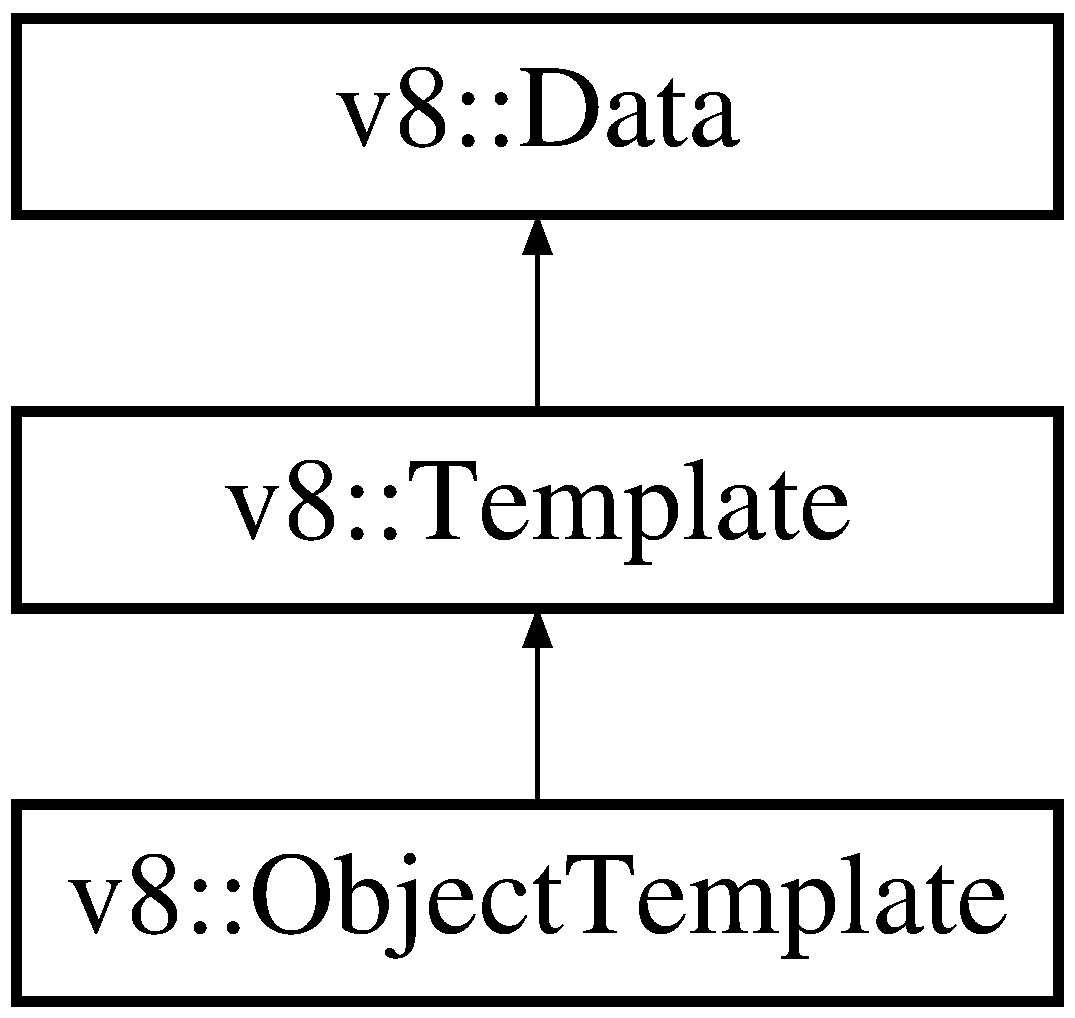
\includegraphics[height=3.000000cm]{classv8_1_1_object_template}
\end{center}
\end{figure}
\subsection*{Public Member Functions}
\begin{DoxyCompactItemize}
\item 
\hyperlink{classv8_1_1_local}{Local}$<$ \hyperlink{classv8_1_1_object}{Object} $>$ \hyperlink{classv8_1_1_object_template_ad25d8ebf37b1a3aaf7d4a03b1a9bd5c1}{New\+Instance} ()
\item 
void \hyperlink{classv8_1_1_object_template_a944ce96b6b65d571f8d682407b70d484}{Set\+Accessor} (\hyperlink{classv8_1_1_handle}{Handle}$<$ \hyperlink{classv8_1_1_string}{String} $>$ name, \hyperlink{namespacev8_a3016fe071826349d1370a700e71be094}{Accessor\+Getter} getter, Accessor\+Setter setter=0, \hyperlink{classv8_1_1_handle}{Handle}$<$ \hyperlink{classv8_1_1_value}{Value} $>$ data=\hyperlink{classv8_1_1_handle}{Handle}$<$ \hyperlink{classv8_1_1_value}{Value} $>$(), \hyperlink{namespacev8_a31d8355cb043d7d2dda3f4a52760b64e}{Access\+Control} settings=D\+E\+F\+A\+U\+L\+T, Property\+Attribute attribute=None)
\item 
void \hyperlink{classv8_1_1_object_template_aa80e9db593d8b954c4153082dc7a439d}{Set\+Named\+Property\+Handler} (\hyperlink{namespacev8_ab9effde41da1c073eddbd4a11a62bd0b}{Named\+Property\+Getter} getter, \hyperlink{namespacev8_a682b1fc46feab32605c4905612ffe870}{Named\+Property\+Setter} setter=0, \hyperlink{namespacev8_a0136e8102c101d9a39497f75daa9153b}{Named\+Property\+Query} query=0, \hyperlink{namespacev8_a7899471fae82b252750b81f41d5c1e26}{Named\+Property\+Deleter} deleter=0, \hyperlink{namespacev8_acbd04b83708cb5a80e73e0396f176e58}{Named\+Property\+Enumerator} enumerator=0, \hyperlink{classv8_1_1_handle}{Handle}$<$ \hyperlink{classv8_1_1_value}{Value} $>$ data=\hyperlink{classv8_1_1_handle}{Handle}$<$ \hyperlink{classv8_1_1_value}{Value} $>$())
\item 
void \hyperlink{classv8_1_1_object_template_af436aeb8132068d3678246f31515ff5a}{Set\+Indexed\+Property\+Handler} (\hyperlink{namespacev8_abf3be19b5157493da3859987cc50c6ab}{Indexed\+Property\+Getter} getter, \hyperlink{namespacev8_a3ca53e294b9b695b3777af904ca942b6}{Indexed\+Property\+Setter} setter=0, \hyperlink{namespacev8_a4b360e915c7c5c1591e946f701d7cc28}{Indexed\+Property\+Query} query=0, \hyperlink{namespacev8_a3a7c18d62a0d1f2d12845051920be592}{Indexed\+Property\+Deleter} deleter=0, \hyperlink{namespacev8_a15ab299eff53946ab483b762a4cb20dc}{Indexed\+Property\+Enumerator} enumerator=0, \hyperlink{classv8_1_1_handle}{Handle}$<$ \hyperlink{classv8_1_1_value}{Value} $>$ data=\hyperlink{classv8_1_1_handle}{Handle}$<$ \hyperlink{classv8_1_1_value}{Value} $>$())
\item 
void \hyperlink{classv8_1_1_object_template_a0132c34bbb52a69d13c54bf325effe6e}{Set\+Call\+As\+Function\+Handler} (Invocation\+Callback callback, \hyperlink{classv8_1_1_handle}{Handle}$<$ \hyperlink{classv8_1_1_value}{Value} $>$ data=\hyperlink{classv8_1_1_handle}{Handle}$<$ \hyperlink{classv8_1_1_value}{Value} $>$())
\item 
void \hyperlink{classv8_1_1_object_template_a7e40ef313b44c2ad336c73051523b4f8}{Mark\+As\+Undetectable} ()
\item 
void \hyperlink{classv8_1_1_object_template_acd0c47ecc715fa1256dc95524a4e8608}{Set\+Access\+Check\+Callbacks} (\hyperlink{namespacev8_ab5cafda0c556bba990c660ce9c904e0d}{Named\+Security\+Callback} named\+\_\+handler, \hyperlink{namespacev8_aebbcc7837753e51112d944ad96520da1}{Indexed\+Security\+Callback} indexed\+\_\+handler, \hyperlink{classv8_1_1_handle}{Handle}$<$ \hyperlink{classv8_1_1_value}{Value} $>$ data=\hyperlink{classv8_1_1_handle}{Handle}$<$ \hyperlink{classv8_1_1_value}{Value} $>$(), bool turned\+\_\+on\+\_\+by\+\_\+default=true)
\item 
int \hyperlink{classv8_1_1_object_template_a43de785d594d8c01b18230b1aa79e31c}{Internal\+Field\+Count} ()
\item 
void \hyperlink{classv8_1_1_object_template_ab63916ac584a76bca8ba541f86ce9fce}{Set\+Internal\+Field\+Count} (int value)
\end{DoxyCompactItemize}
\subsection*{Static Public Member Functions}
\begin{DoxyCompactItemize}
\item 
static \hyperlink{classv8_1_1_local}{Local}$<$ \hyperlink{classv8_1_1_object_template}{Object\+Template} $>$ \hyperlink{classv8_1_1_object_template_a394801526a9e9eb6df349a0eb8dfa0d0}{New} ()
\end{DoxyCompactItemize}
\subsection*{Friends}
\begin{DoxyCompactItemize}
\item 
\hypertarget{classv8_1_1_object_template_a334168ad1a5f39cf17b818ca3356aacd}{}class {\bfseries Function\+Template}\label{classv8_1_1_object_template_a334168ad1a5f39cf17b818ca3356aacd}

\end{DoxyCompactItemize}


\subsection{Detailed Description}
An \hyperlink{classv8_1_1_object_template}{Object\+Template} is used to create objects at runtime.

Properties added to an \hyperlink{classv8_1_1_object_template}{Object\+Template} are added to each object created from the \hyperlink{classv8_1_1_object_template}{Object\+Template}. 

\subsection{Member Function Documentation}
\hypertarget{classv8_1_1_object_template_a43de785d594d8c01b18230b1aa79e31c}{}\index{v8\+::\+Object\+Template@{v8\+::\+Object\+Template}!Internal\+Field\+Count@{Internal\+Field\+Count}}
\index{Internal\+Field\+Count@{Internal\+Field\+Count}!v8\+::\+Object\+Template@{v8\+::\+Object\+Template}}
\subsubsection[{Internal\+Field\+Count}]{\setlength{\rightskip}{0pt plus 5cm}int v8\+::\+Object\+Template\+::\+Internal\+Field\+Count (
\begin{DoxyParamCaption}
{}
\end{DoxyParamCaption}
)}\label{classv8_1_1_object_template_a43de785d594d8c01b18230b1aa79e31c}
Gets the number of internal fields for objects generated from this template. \hypertarget{classv8_1_1_object_template_a7e40ef313b44c2ad336c73051523b4f8}{}\index{v8\+::\+Object\+Template@{v8\+::\+Object\+Template}!Mark\+As\+Undetectable@{Mark\+As\+Undetectable}}
\index{Mark\+As\+Undetectable@{Mark\+As\+Undetectable}!v8\+::\+Object\+Template@{v8\+::\+Object\+Template}}
\subsubsection[{Mark\+As\+Undetectable}]{\setlength{\rightskip}{0pt plus 5cm}void v8\+::\+Object\+Template\+::\+Mark\+As\+Undetectable (
\begin{DoxyParamCaption}
{}
\end{DoxyParamCaption}
)}\label{classv8_1_1_object_template_a7e40ef313b44c2ad336c73051523b4f8}
Mark object instances of the template as undetectable.

In many ways, undetectable objects behave as though they are not there. They behave like \textquotesingle{}undefined\textquotesingle{} in conditionals and when printed. However, properties can be accessed and called as on normal objects. \hypertarget{classv8_1_1_object_template_a394801526a9e9eb6df349a0eb8dfa0d0}{}\index{v8\+::\+Object\+Template@{v8\+::\+Object\+Template}!New@{New}}
\index{New@{New}!v8\+::\+Object\+Template@{v8\+::\+Object\+Template}}
\subsubsection[{New}]{\setlength{\rightskip}{0pt plus 5cm}static {\bf Local}$<${\bf Object\+Template}$>$ v8\+::\+Object\+Template\+::\+New (
\begin{DoxyParamCaption}
{}
\end{DoxyParamCaption}
)\hspace{0.3cm}{\ttfamily [static]}}\label{classv8_1_1_object_template_a394801526a9e9eb6df349a0eb8dfa0d0}
Creates an \hyperlink{classv8_1_1_object_template}{Object\+Template}. \hypertarget{classv8_1_1_object_template_ad25d8ebf37b1a3aaf7d4a03b1a9bd5c1}{}\index{v8\+::\+Object\+Template@{v8\+::\+Object\+Template}!New\+Instance@{New\+Instance}}
\index{New\+Instance@{New\+Instance}!v8\+::\+Object\+Template@{v8\+::\+Object\+Template}}
\subsubsection[{New\+Instance}]{\setlength{\rightskip}{0pt plus 5cm}{\bf Local}$<${\bf Object}$>$ v8\+::\+Object\+Template\+::\+New\+Instance (
\begin{DoxyParamCaption}
{}
\end{DoxyParamCaption}
)}\label{classv8_1_1_object_template_ad25d8ebf37b1a3aaf7d4a03b1a9bd5c1}
Creates a new instance of this template. \hypertarget{classv8_1_1_object_template_acd0c47ecc715fa1256dc95524a4e8608}{}\index{v8\+::\+Object\+Template@{v8\+::\+Object\+Template}!Set\+Access\+Check\+Callbacks@{Set\+Access\+Check\+Callbacks}}
\index{Set\+Access\+Check\+Callbacks@{Set\+Access\+Check\+Callbacks}!v8\+::\+Object\+Template@{v8\+::\+Object\+Template}}
\subsubsection[{Set\+Access\+Check\+Callbacks}]{\setlength{\rightskip}{0pt plus 5cm}void v8\+::\+Object\+Template\+::\+Set\+Access\+Check\+Callbacks (
\begin{DoxyParamCaption}
\item[{{\bf Named\+Security\+Callback}}]{named\+\_\+handler, }
\item[{{\bf Indexed\+Security\+Callback}}]{indexed\+\_\+handler, }
\item[{{\bf Handle}$<$ {\bf Value} $>$}]{data = {\ttfamily {\bf Handle}$<$~{\bf Value}~$>$()}, }
\item[{bool}]{turned\+\_\+on\+\_\+by\+\_\+default = {\ttfamily true}}
\end{DoxyParamCaption}
)}\label{classv8_1_1_object_template_acd0c47ecc715fa1256dc95524a4e8608}
Sets access check callbacks on the object template.

When accessing properties on instances of this object template, the access check callback will be called to determine whether or not to allow cross-\/context access to the properties. The last parameter specifies whether access checks are turned on by default on instances. If access checks are off by default, they can be turned on on individual instances by calling \hyperlink{classv8_1_1_object_a6e9fe342c0f77995defa6b479d01a3bd}{Object\+::\+Turn\+On\+Access\+Check()}. \hypertarget{classv8_1_1_object_template_a944ce96b6b65d571f8d682407b70d484}{}\index{v8\+::\+Object\+Template@{v8\+::\+Object\+Template}!Set\+Accessor@{Set\+Accessor}}
\index{Set\+Accessor@{Set\+Accessor}!v8\+::\+Object\+Template@{v8\+::\+Object\+Template}}
\subsubsection[{Set\+Accessor}]{\setlength{\rightskip}{0pt plus 5cm}void v8\+::\+Object\+Template\+::\+Set\+Accessor (
\begin{DoxyParamCaption}
\item[{{\bf Handle}$<$ {\bf String} $>$}]{name, }
\item[{{\bf Accessor\+Getter}}]{getter, }
\item[{Accessor\+Setter}]{setter = {\ttfamily 0}, }
\item[{{\bf Handle}$<$ {\bf Value} $>$}]{data = {\ttfamily {\bf Handle}$<$~{\bf Value}~$>$()}, }
\item[{{\bf Access\+Control}}]{settings = {\ttfamily DEFAULT}, }
\item[{Property\+Attribute}]{attribute = {\ttfamily None}}
\end{DoxyParamCaption}
)}\label{classv8_1_1_object_template_a944ce96b6b65d571f8d682407b70d484}
Sets an accessor on the object template.

Whenever the property with the given name is accessed on objects created from this \hyperlink{classv8_1_1_object_template}{Object\+Template} the getter and setter callbacks are called instead of getting and setting the property directly on the Java\+Script object.


\begin{DoxyParams}{Parameters}
{\em name} & The name of the property for which an accessor is added. \\
\hline
{\em getter} & The callback to invoke when getting the property. \\
\hline
{\em setter} & The callback to invoke when setting the property. \\
\hline
{\em data} & A piece of data that will be passed to the getter and setter callbacks whenever they are invoked. \\
\hline
{\em settings} & Access control settings for the accessor. This is a bit field consisting of one of more of D\+E\+F\+A\+U\+L\+T = 0, A\+L\+L\+\_\+\+C\+A\+N\+\_\+\+R\+E\+A\+D = 1, or A\+L\+L\+\_\+\+C\+A\+N\+\_\+\+W\+R\+I\+T\+E = 2. The default is to not allow cross-\/context access. A\+L\+L\+\_\+\+C\+A\+N\+\_\+\+R\+E\+A\+D means that all cross-\/context reads are allowed. A\+L\+L\+\_\+\+C\+A\+N\+\_\+\+W\+R\+I\+T\+E means that all cross-\/context writes are allowed. The combination A\+L\+L\+\_\+\+C\+A\+N\+\_\+\+R\+E\+A\+D $\vert$ A\+L\+L\+\_\+\+C\+A\+N\+\_\+\+W\+R\+I\+T\+E can be used to allow all cross-\/context access. \\
\hline
{\em attribute} & The attributes of the property for which an accessor is added. \\
\hline
\end{DoxyParams}
\hypertarget{classv8_1_1_object_template_a0132c34bbb52a69d13c54bf325effe6e}{}\index{v8\+::\+Object\+Template@{v8\+::\+Object\+Template}!Set\+Call\+As\+Function\+Handler@{Set\+Call\+As\+Function\+Handler}}
\index{Set\+Call\+As\+Function\+Handler@{Set\+Call\+As\+Function\+Handler}!v8\+::\+Object\+Template@{v8\+::\+Object\+Template}}
\subsubsection[{Set\+Call\+As\+Function\+Handler}]{\setlength{\rightskip}{0pt plus 5cm}void v8\+::\+Object\+Template\+::\+Set\+Call\+As\+Function\+Handler (
\begin{DoxyParamCaption}
\item[{Invocation\+Callback}]{callback, }
\item[{{\bf Handle}$<$ {\bf Value} $>$}]{data = {\ttfamily {\bf Handle}$<$~{\bf Value}~$>$()}}
\end{DoxyParamCaption}
)}\label{classv8_1_1_object_template_a0132c34bbb52a69d13c54bf325effe6e}
Sets the callback to be used when calling instances created from this template as a function. If no callback is set, instances behave like normal Java\+Script objects that cannot be called as a function. \hypertarget{classv8_1_1_object_template_af436aeb8132068d3678246f31515ff5a}{}\index{v8\+::\+Object\+Template@{v8\+::\+Object\+Template}!Set\+Indexed\+Property\+Handler@{Set\+Indexed\+Property\+Handler}}
\index{Set\+Indexed\+Property\+Handler@{Set\+Indexed\+Property\+Handler}!v8\+::\+Object\+Template@{v8\+::\+Object\+Template}}
\subsubsection[{Set\+Indexed\+Property\+Handler}]{\setlength{\rightskip}{0pt plus 5cm}void v8\+::\+Object\+Template\+::\+Set\+Indexed\+Property\+Handler (
\begin{DoxyParamCaption}
\item[{{\bf Indexed\+Property\+Getter}}]{getter, }
\item[{{\bf Indexed\+Property\+Setter}}]{setter = {\ttfamily 0}, }
\item[{{\bf Indexed\+Property\+Query}}]{query = {\ttfamily 0}, }
\item[{{\bf Indexed\+Property\+Deleter}}]{deleter = {\ttfamily 0}, }
\item[{{\bf Indexed\+Property\+Enumerator}}]{enumerator = {\ttfamily 0}, }
\item[{{\bf Handle}$<$ {\bf Value} $>$}]{data = {\ttfamily {\bf Handle}$<$~{\bf Value}~$>$()}}
\end{DoxyParamCaption}
)}\label{classv8_1_1_object_template_af436aeb8132068d3678246f31515ff5a}
Sets an indexed property handler on the object template.

Whenever an indexed property is accessed on objects created from this object template, the provided callback is invoked instead of accessing the property directly on the Java\+Script object.


\begin{DoxyParams}{Parameters}
{\em getter} & The callback to invoke when getting a property. \\
\hline
{\em setter} & The callback to invoke when setting a property. \\
\hline
{\em query} & The callback to invoke to check is an object has a property. \\
\hline
{\em deleter} & The callback to invoke when deleting a property. \\
\hline
{\em enumerator} & The callback to invoke to enumerate all the indexed properties of an object. \\
\hline
{\em data} & A piece of data that will be passed to the callbacks whenever they are invoked. \\
\hline
\end{DoxyParams}
\hypertarget{classv8_1_1_object_template_ab63916ac584a76bca8ba541f86ce9fce}{}\index{v8\+::\+Object\+Template@{v8\+::\+Object\+Template}!Set\+Internal\+Field\+Count@{Set\+Internal\+Field\+Count}}
\index{Set\+Internal\+Field\+Count@{Set\+Internal\+Field\+Count}!v8\+::\+Object\+Template@{v8\+::\+Object\+Template}}
\subsubsection[{Set\+Internal\+Field\+Count}]{\setlength{\rightskip}{0pt plus 5cm}void v8\+::\+Object\+Template\+::\+Set\+Internal\+Field\+Count (
\begin{DoxyParamCaption}
\item[{int}]{value}
\end{DoxyParamCaption}
)}\label{classv8_1_1_object_template_ab63916ac584a76bca8ba541f86ce9fce}
Sets the number of internal fields for objects generated from this template. \hypertarget{classv8_1_1_object_template_aa80e9db593d8b954c4153082dc7a439d}{}\index{v8\+::\+Object\+Template@{v8\+::\+Object\+Template}!Set\+Named\+Property\+Handler@{Set\+Named\+Property\+Handler}}
\index{Set\+Named\+Property\+Handler@{Set\+Named\+Property\+Handler}!v8\+::\+Object\+Template@{v8\+::\+Object\+Template}}
\subsubsection[{Set\+Named\+Property\+Handler}]{\setlength{\rightskip}{0pt plus 5cm}void v8\+::\+Object\+Template\+::\+Set\+Named\+Property\+Handler (
\begin{DoxyParamCaption}
\item[{{\bf Named\+Property\+Getter}}]{getter, }
\item[{{\bf Named\+Property\+Setter}}]{setter = {\ttfamily 0}, }
\item[{{\bf Named\+Property\+Query}}]{query = {\ttfamily 0}, }
\item[{{\bf Named\+Property\+Deleter}}]{deleter = {\ttfamily 0}, }
\item[{{\bf Named\+Property\+Enumerator}}]{enumerator = {\ttfamily 0}, }
\item[{{\bf Handle}$<$ {\bf Value} $>$}]{data = {\ttfamily {\bf Handle}$<$~{\bf Value}~$>$()}}
\end{DoxyParamCaption}
)}\label{classv8_1_1_object_template_aa80e9db593d8b954c4153082dc7a439d}
Sets a named property handler on the object template.

Whenever a named property is accessed on objects created from this object template, the provided callback is invoked instead of accessing the property directly on the Java\+Script object.


\begin{DoxyParams}{Parameters}
{\em getter} & The callback to invoke when getting a property. \\
\hline
{\em setter} & The callback to invoke when setting a property. \\
\hline
{\em query} & The callback to invoke to check if a property is present, and if present, get its attributes. \\
\hline
{\em deleter} & The callback to invoke when deleting a property. \\
\hline
{\em enumerator} & The callback to invoke to enumerate all the named properties of an object. \\
\hline
{\em data} & A piece of data that will be passed to the callbacks whenever they are invoked. \\
\hline
\end{DoxyParams}


The documentation for this class was generated from the following file\+:\begin{DoxyCompactItemize}
\item 
deps/v8/include/v8.\+h\end{DoxyCompactItemize}

\hypertarget{classv8_1_1_output_stream}{}\section{v8\+:\+:Output\+Stream Class Reference}
\label{classv8_1_1_output_stream}\index{v8\+::\+Output\+Stream@{v8\+::\+Output\+Stream}}


{\ttfamily \#include $<$v8-\/profiler.\+h$>$}

\subsection*{Public Types}
\begin{DoxyCompactItemize}
\item 
\hypertarget{classv8_1_1_output_stream_a336c7605a0ce4fbe6f6fca3b03bc16de}{}enum {\bfseries Write\+Result} \{ {\bfseries k\+Continue} = 0, 
{\bfseries k\+Abort} = 1
 \}\label{classv8_1_1_output_stream_a336c7605a0ce4fbe6f6fca3b03bc16de}

\end{DoxyCompactItemize}
\subsection*{Public Member Functions}
\begin{DoxyCompactItemize}
\item 
virtual void \hyperlink{classv8_1_1_output_stream_a6c5c308367fc5776bcbedff0e94d6049}{End\+Of\+Stream} ()=0
\item 
virtual int \hyperlink{classv8_1_1_output_stream_a93bdaa790cbd66a7283fad2cca3f48f7}{Get\+Chunk\+Size} ()
\item 
virtual Write\+Result \hyperlink{classv8_1_1_output_stream_a42adc62ebe43d00159f80328538f217f}{Write\+Ascii\+Chunk} (char $\ast$data, int size)=0
\item 
virtual Write\+Result \hyperlink{classv8_1_1_output_stream_a104fd1a0b5ef685e1d4967aaacbb9e9d}{Write\+Heap\+Stats\+Chunk} (\hyperlink{structv8_1_1_heap_stats_update}{Heap\+Stats\+Update} $\ast$data, int count)
\end{DoxyCompactItemize}


\subsection{Detailed Description}
An interface for exporting data from \hyperlink{classv8_1_1_v8}{V8}, using \char`\"{}push\char`\"{} model. 

\subsection{Member Function Documentation}
\hypertarget{classv8_1_1_output_stream_a6c5c308367fc5776bcbedff0e94d6049}{}\index{v8\+::\+Output\+Stream@{v8\+::\+Output\+Stream}!End\+Of\+Stream@{End\+Of\+Stream}}
\index{End\+Of\+Stream@{End\+Of\+Stream}!v8\+::\+Output\+Stream@{v8\+::\+Output\+Stream}}
\subsubsection[{End\+Of\+Stream}]{\setlength{\rightskip}{0pt plus 5cm}virtual void v8\+::\+Output\+Stream\+::\+End\+Of\+Stream (
\begin{DoxyParamCaption}
{}
\end{DoxyParamCaption}
)\hspace{0.3cm}{\ttfamily [pure virtual]}}\label{classv8_1_1_output_stream_a6c5c308367fc5776bcbedff0e94d6049}
Notify about the end of stream. \hypertarget{classv8_1_1_output_stream_a93bdaa790cbd66a7283fad2cca3f48f7}{}\index{v8\+::\+Output\+Stream@{v8\+::\+Output\+Stream}!Get\+Chunk\+Size@{Get\+Chunk\+Size}}
\index{Get\+Chunk\+Size@{Get\+Chunk\+Size}!v8\+::\+Output\+Stream@{v8\+::\+Output\+Stream}}
\subsubsection[{Get\+Chunk\+Size}]{\setlength{\rightskip}{0pt plus 5cm}virtual int v8\+::\+Output\+Stream\+::\+Get\+Chunk\+Size (
\begin{DoxyParamCaption}
{}
\end{DoxyParamCaption}
)\hspace{0.3cm}{\ttfamily [inline]}, {\ttfamily [virtual]}}\label{classv8_1_1_output_stream_a93bdaa790cbd66a7283fad2cca3f48f7}
Get preferred output chunk size. Called only once. \hypertarget{classv8_1_1_output_stream_a42adc62ebe43d00159f80328538f217f}{}\index{v8\+::\+Output\+Stream@{v8\+::\+Output\+Stream}!Write\+Ascii\+Chunk@{Write\+Ascii\+Chunk}}
\index{Write\+Ascii\+Chunk@{Write\+Ascii\+Chunk}!v8\+::\+Output\+Stream@{v8\+::\+Output\+Stream}}
\subsubsection[{Write\+Ascii\+Chunk}]{\setlength{\rightskip}{0pt plus 5cm}virtual Write\+Result v8\+::\+Output\+Stream\+::\+Write\+Ascii\+Chunk (
\begin{DoxyParamCaption}
\item[{char $\ast$}]{data, }
\item[{int}]{size}
\end{DoxyParamCaption}
)\hspace{0.3cm}{\ttfamily [pure virtual]}}\label{classv8_1_1_output_stream_a42adc62ebe43d00159f80328538f217f}
Writes the next chunk of snapshot data into the stream. Writing can be stopped by returning k\+Abort as function result. End\+Of\+Stream will not be called in case writing was aborted. \hypertarget{classv8_1_1_output_stream_a104fd1a0b5ef685e1d4967aaacbb9e9d}{}\index{v8\+::\+Output\+Stream@{v8\+::\+Output\+Stream}!Write\+Heap\+Stats\+Chunk@{Write\+Heap\+Stats\+Chunk}}
\index{Write\+Heap\+Stats\+Chunk@{Write\+Heap\+Stats\+Chunk}!v8\+::\+Output\+Stream@{v8\+::\+Output\+Stream}}
\subsubsection[{Write\+Heap\+Stats\+Chunk}]{\setlength{\rightskip}{0pt plus 5cm}virtual Write\+Result v8\+::\+Output\+Stream\+::\+Write\+Heap\+Stats\+Chunk (
\begin{DoxyParamCaption}
\item[{{\bf Heap\+Stats\+Update} $\ast$}]{data, }
\item[{int}]{count}
\end{DoxyParamCaption}
)\hspace{0.3cm}{\ttfamily [inline]}, {\ttfamily [virtual]}}\label{classv8_1_1_output_stream_a104fd1a0b5ef685e1d4967aaacbb9e9d}
Writes the next chunk of heap stats data into the stream. Writing can be stopped by returning k\+Abort as function result. End\+Of\+Stream will not be called in case writing was aborted. 

The documentation for this class was generated from the following file\+:\begin{DoxyCompactItemize}
\item 
deps/v8/include/v8-\/profiler.\+h\end{DoxyCompactItemize}

\hypertarget{classv8_1_1_persistent}{}\section{v8\+:\+:Persistent$<$ T $>$ Class Template Reference}
\label{classv8_1_1_persistent}\index{v8\+::\+Persistent$<$ T $>$@{v8\+::\+Persistent$<$ T $>$}}


{\ttfamily \#include $<$v8.\+h$>$}

Inheritance diagram for v8\+:\+:Persistent$<$ T $>$\+:\begin{figure}[H]
\begin{center}
\leavevmode
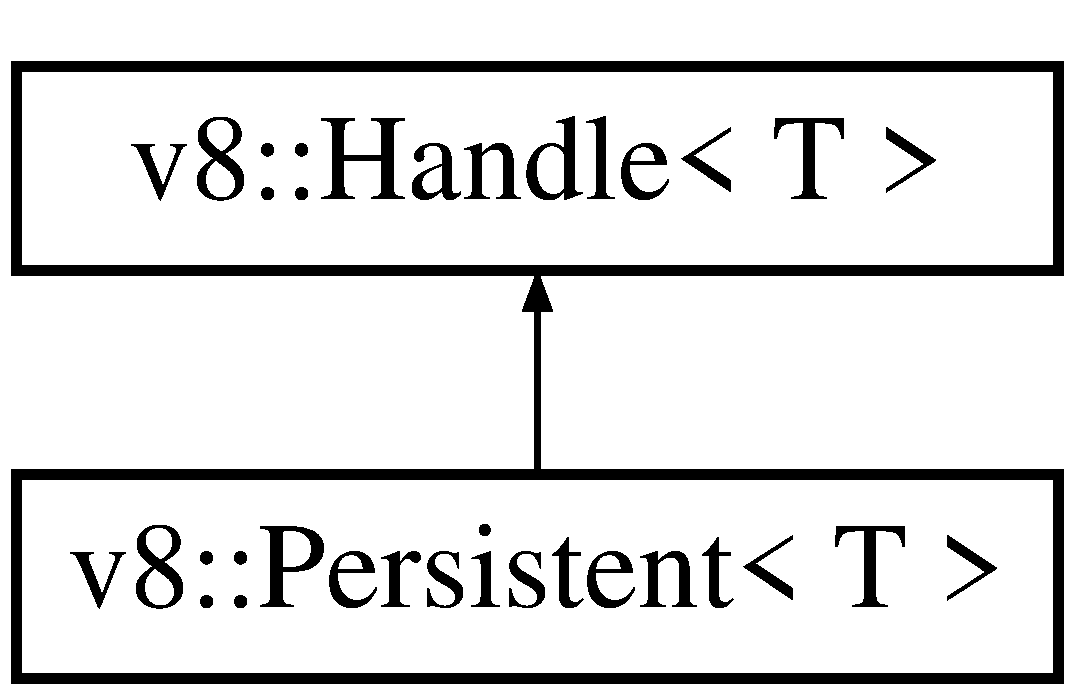
\includegraphics[height=2.000000cm]{classv8_1_1_persistent}
\end{center}
\end{figure}
\subsection*{Public Member Functions}
\begin{DoxyCompactItemize}
\item 
\hyperlink{classv8_1_1_persistent_ad523a6fc8bf2490020009436519423d0}{V8\+\_\+\+I\+N\+L\+I\+N\+E} (\hyperlink{classv8_1_1_persistent}{Persistent}())
\item 
{\footnotesize template$<$class S $>$ }\\\hyperlink{classv8_1_1_persistent_a22ac4d575e808ed10b6504dc8f812789}{V8\+\_\+\+I\+N\+L\+I\+N\+E} (\hyperlink{classv8_1_1_persistent}{Persistent}(\hyperlink{classv8_1_1_persistent}{Persistent}$<$ S $>$ that))
\item 
\hypertarget{classv8_1_1_persistent_a59285008a6fcdd9a5189015403375b4e}{}{\footnotesize template$<$class S $>$ }\\{\bfseries V8\+\_\+\+I\+N\+L\+I\+N\+E} (\hyperlink{classv8_1_1_persistent}{Persistent}(S $\ast$that))\label{classv8_1_1_persistent_a59285008a6fcdd9a5189015403375b4e}

\item 
{\footnotesize template$<$class S $>$ }\\\hyperlink{classv8_1_1_persistent_aabe20913d6860e124574bc4d67535a5c}{V8\+\_\+\+I\+N\+L\+I\+N\+E} (\hyperlink{classv8_1_1_persistent}{Persistent}(\hyperlink{classv8_1_1_handle}{Handle}$<$ S $>$ that))
\item 
\hypertarget{classv8_1_1_persistent_acd5e8f1e94848aff791b9bdf0f1fed90}{}{\footnotesize template$<$class S $>$ }\\{\bfseries V8\+\_\+\+I\+N\+L\+I\+N\+E} (static \hyperlink{classv8_1_1_persistent}{Persistent}$<$ T $>$ Cast(\hyperlink{classv8_1_1_persistent}{Persistent}$<$ S $>$ that))\label{classv8_1_1_persistent_acd5e8f1e94848aff791b9bdf0f1fed90}

\item 
\hypertarget{classv8_1_1_persistent_a092bc149b5515c88e5950717e90eed9f}{}{\footnotesize template$<$class S $>$ }\\{\bfseries V8\+\_\+\+I\+N\+L\+I\+N\+E} (\hyperlink{classv8_1_1_persistent}{Persistent}$<$ S $>$ As())\label{classv8_1_1_persistent_a092bc149b5515c88e5950717e90eed9f}

\item 
\hyperlink{classv8_1_1_persistent_a6f6e0d5627191c9e45f4cb63ef8b805d}{V8\+\_\+\+I\+N\+L\+I\+N\+E} (static \hyperlink{classv8_1_1_persistent}{Persistent}$<$ T $>$ New(\hyperlink{classv8_1_1_handle}{Handle}$<$ T $>$ that))
\item 
\hyperlink{classv8_1_1_persistent_adae44eb24d3c568f9ab948d3efd3dbfa}{V8\+\_\+\+I\+N\+L\+I\+N\+E} (void Dispose())
\item 
\hypertarget{classv8_1_1_persistent_aa0f3928a4dd02a35d174299346673846}{}{\bfseries V8\+\_\+\+I\+N\+L\+I\+N\+E} (void Dispose(\hyperlink{classv8_1_1_isolate}{Isolate} $\ast$isolate))\label{classv8_1_1_persistent_aa0f3928a4dd02a35d174299346673846}

\item 
\hyperlink{classv8_1_1_persistent_ab50a6cc3922980d86ef692e4a460d459}{V8\+\_\+\+I\+N\+L\+I\+N\+E} (void Make\+Weak(void $\ast$parameters, \hyperlink{namespacev8_a4d5db775dbc002b23f1b55ec7ce80ea5}{Weak\+Reference\+Callback} callback))
\item 
\hypertarget{classv8_1_1_persistent_a3b4deee5bd1f9f1d8149b3bdce1449a3}{}{\bfseries V8\+\_\+\+I\+N\+L\+I\+N\+E} (void Make\+Weak(\hyperlink{classv8_1_1_isolate}{Isolate} $\ast$isolate, void $\ast$parameters, \hyperlink{namespacev8_a4d5db775dbc002b23f1b55ec7ce80ea5}{Weak\+Reference\+Callback} callback))\label{classv8_1_1_persistent_a3b4deee5bd1f9f1d8149b3bdce1449a3}

\item 
\hyperlink{classv8_1_1_persistent_aef009f9e3c6e0ac21cdbad2907686ac3}{V8\+\_\+\+I\+N\+L\+I\+N\+E} (void Clear\+Weak())
\item 
\hyperlink{classv8_1_1_persistent_aa8497281225e9678f03b6997ae559960}{V8\+\_\+\+I\+N\+L\+I\+N\+E} (void Mark\+Independent())
\item 
\hypertarget{classv8_1_1_persistent_a2b4071c032c97886ba1bcb0ebacb2209}{}{\bfseries V8\+\_\+\+I\+N\+L\+I\+N\+E} (void Mark\+Independent(\hyperlink{classv8_1_1_isolate}{Isolate} $\ast$isolate))\label{classv8_1_1_persistent_a2b4071c032c97886ba1bcb0ebacb2209}

\item 
\hyperlink{classv8_1_1_persistent_ab096f22fc5023ba07631537633b42565}{V8\+\_\+\+I\+N\+L\+I\+N\+E} (void Mark\+Partially\+Dependent())
\item 
\hypertarget{classv8_1_1_persistent_a89a708d5a98331a2683324be9dc5a474}{}{\bfseries V8\+\_\+\+I\+N\+L\+I\+N\+E} (void Mark\+Partially\+Dependent(\hyperlink{classv8_1_1_isolate}{Isolate} $\ast$isolate))\label{classv8_1_1_persistent_a89a708d5a98331a2683324be9dc5a474}

\item 
\hyperlink{classv8_1_1_persistent_ae63945077238e19dbe1566c316c1c774}{V8\+\_\+\+I\+N\+L\+I\+N\+E} (bool Is\+Independent() const)
\item 
\hypertarget{classv8_1_1_persistent_a0cb1529e8138c0072f6efac79056e225}{}{\bfseries V8\+\_\+\+I\+N\+L\+I\+N\+E} (bool Is\+Independent(\hyperlink{classv8_1_1_isolate}{Isolate} $\ast$isolate) const)\label{classv8_1_1_persistent_a0cb1529e8138c0072f6efac79056e225}

\item 
\hyperlink{classv8_1_1_persistent_a480643005f3ce865ea6084a9249dbf6f}{V8\+\_\+\+I\+N\+L\+I\+N\+E} (bool Is\+Near\+Death() const)
\item 
\hyperlink{classv8_1_1_persistent_ab3ecacdf4c67a295d57658e348153b6c}{V8\+\_\+\+I\+N\+L\+I\+N\+E} (bool Is\+Weak() const)
\item 
\hypertarget{classv8_1_1_persistent_acfa08355e94e227b6319123d40cd8710}{}{\bfseries V8\+\_\+\+I\+N\+L\+I\+N\+E} (bool Is\+Weak(\hyperlink{classv8_1_1_isolate}{Isolate} $\ast$isolate) const)\label{classv8_1_1_persistent_acfa08355e94e227b6319123d40cd8710}

\item 
\hyperlink{classv8_1_1_persistent_a57a08d23ba324fee6b86e4df808e1d6d}{V8\+\_\+\+I\+N\+L\+I\+N\+E} (void Set\+Wrapper\+Class\+Id(uint16\+\_\+t class\+\_\+id))
\item 
\hyperlink{classv8_1_1_persistent_aea12008dfeca52acd8e687187c25e4b7}{V8\+\_\+\+I\+N\+L\+I\+N\+E} (uint16\+\_\+t Wrapper\+Class\+Id() const)
\end{DoxyCompactItemize}
\subsection*{Friends}
\begin{DoxyCompactItemize}
\item 
\hypertarget{classv8_1_1_persistent_ac7b520085953e146d849e05253267f72}{}class {\bfseries Implementation\+Utilities}\label{classv8_1_1_persistent_ac7b520085953e146d849e05253267f72}

\item 
\hypertarget{classv8_1_1_persistent_a4d28646409234f556983be8a96c06424}{}class {\bfseries Object\+Template}\label{classv8_1_1_persistent_a4d28646409234f556983be8a96c06424}

\end{DoxyCompactItemize}


\subsection{Detailed Description}
\subsubsection*{template$<$class T$>$class v8\+::\+Persistent$<$ T $>$}

An object reference that is independent of any handle scope. Where a \hyperlink{classv8_1_1_local}{Local} handle only lives as long as the \hyperlink{classv8_1_1_handle_scope}{Handle\+Scope} in which it was allocated, a \hyperlink{classv8_1_1_persistent}{Persistent} handle remains valid until it is explicitly disposed.

A persistent handle contains a reference to a storage cell within the \hyperlink{namespacev8}{v8} engine which holds an object value and which is updated by the garbage collector whenever the object is moved. A new storage cell can be created using Persistent\+::\+New and existing handles can be disposed using Persistent\+::\+Dispose. Since persistent handles are passed by value you may have many persistent handle objects that point to the same storage cell. For instance, if you pass a persistent handle as an argument to a function you will not get two different storage cells but rather two references to the same storage cell. 

\subsection{Member Function Documentation}
\hypertarget{classv8_1_1_persistent_ad523a6fc8bf2490020009436519423d0}{}\index{v8\+::\+Persistent@{v8\+::\+Persistent}!V8\+\_\+\+I\+N\+L\+I\+N\+E@{V8\+\_\+\+I\+N\+L\+I\+N\+E}}
\index{V8\+\_\+\+I\+N\+L\+I\+N\+E@{V8\+\_\+\+I\+N\+L\+I\+N\+E}!v8\+::\+Persistent@{v8\+::\+Persistent}}
\subsubsection[{V8\+\_\+\+I\+N\+L\+I\+N\+E}]{\setlength{\rightskip}{0pt plus 5cm}template$<$class T $>$ {\bf v8\+::\+Persistent}$<$ T $>$\+::V8\+\_\+\+I\+N\+L\+I\+N\+E (
\begin{DoxyParamCaption}
\item[{{\bf Persistent}$<$ T $>$()}]{}
\end{DoxyParamCaption}
)}\label{classv8_1_1_persistent_ad523a6fc8bf2490020009436519423d0}
Creates an empty persistent handle that doesn\textquotesingle{}t point to any storage cell. \hypertarget{classv8_1_1_persistent_a22ac4d575e808ed10b6504dc8f812789}{}\index{v8\+::\+Persistent@{v8\+::\+Persistent}!V8\+\_\+\+I\+N\+L\+I\+N\+E@{V8\+\_\+\+I\+N\+L\+I\+N\+E}}
\index{V8\+\_\+\+I\+N\+L\+I\+N\+E@{V8\+\_\+\+I\+N\+L\+I\+N\+E}!v8\+::\+Persistent@{v8\+::\+Persistent}}
\subsubsection[{V8\+\_\+\+I\+N\+L\+I\+N\+E}]{\setlength{\rightskip}{0pt plus 5cm}template$<$class T $>$ template$<$class S $>$ {\bf v8\+::\+Persistent}$<$ T $>$\+::V8\+\_\+\+I\+N\+L\+I\+N\+E (
\begin{DoxyParamCaption}
\item[{{\bf Persistent}$<$ T $>$({\bf Persistent}$<$ S $>$ that)     }]{}
\end{DoxyParamCaption}
)\hspace{0.3cm}{\ttfamily [inline]}}\label{classv8_1_1_persistent_a22ac4d575e808ed10b6504dc8f812789}
Creates a persistent handle for the same storage cell as the specified handle. This constructor allows you to pass persistent handles as arguments by value and to assign between persistent handles. However, attempting to assign between incompatible persistent handles, for instance from a Persistent$<$\+String$>$ to a Persistent$<$\+Number$>$ will cause a compile-\/time error. Assigning between compatible persistent handles, for instance assigning a Persistent$<$\+String$>$ to a variable declared as Persistent$<$\+Value$>$, is allowed as \hyperlink{classv8_1_1_string}{String} is a subclass of \hyperlink{classv8_1_1_value}{Value}. This check fails when trying to convert between incompatible handles. For example, converting from a Handle$<$\+String$>$ to a Handle$<$\+Number$>$.\hypertarget{classv8_1_1_persistent_aabe20913d6860e124574bc4d67535a5c}{}\index{v8\+::\+Persistent@{v8\+::\+Persistent}!V8\+\_\+\+I\+N\+L\+I\+N\+E@{V8\+\_\+\+I\+N\+L\+I\+N\+E}}
\index{V8\+\_\+\+I\+N\+L\+I\+N\+E@{V8\+\_\+\+I\+N\+L\+I\+N\+E}!v8\+::\+Persistent@{v8\+::\+Persistent}}
\subsubsection[{V8\+\_\+\+I\+N\+L\+I\+N\+E}]{\setlength{\rightskip}{0pt plus 5cm}template$<$class T $>$ template$<$class S $>$ {\bf v8\+::\+Persistent}$<$ T $>$\+::V8\+\_\+\+I\+N\+L\+I\+N\+E (
\begin{DoxyParamCaption}
\item[{{\bf Persistent}$<$ T $>$({\bf Handle}$<$ S $>$ that)     }]{}
\end{DoxyParamCaption}
)\hspace{0.3cm}{\ttfamily [inline]}, {\ttfamily [explicit]}}\label{classv8_1_1_persistent_aabe20913d6860e124574bc4d67535a5c}
\char`\"{}\+Casts\char`\"{} a plain handle which is known to be a persistent handle to a persistent handle. \hypertarget{classv8_1_1_persistent_a6f6e0d5627191c9e45f4cb63ef8b805d}{}\index{v8\+::\+Persistent@{v8\+::\+Persistent}!V8\+\_\+\+I\+N\+L\+I\+N\+E@{V8\+\_\+\+I\+N\+L\+I\+N\+E}}
\index{V8\+\_\+\+I\+N\+L\+I\+N\+E@{V8\+\_\+\+I\+N\+L\+I\+N\+E}!v8\+::\+Persistent@{v8\+::\+Persistent}}
\subsubsection[{V8\+\_\+\+I\+N\+L\+I\+N\+E}]{\setlength{\rightskip}{0pt plus 5cm}template$<$class T $>$ {\bf v8\+::\+Persistent}$<$ T $>$\+::V8\+\_\+\+I\+N\+L\+I\+N\+E (
\begin{DoxyParamCaption}
\item[{static {\bf Persistent}$<$ T $>$ }]{NewHandle$<$ T $>$ that}
\end{DoxyParamCaption}
)}\label{classv8_1_1_persistent_a6f6e0d5627191c9e45f4cb63ef8b805d}
Creates a new persistent handle for an existing local or persistent handle. \hypertarget{classv8_1_1_persistent_adae44eb24d3c568f9ab948d3efd3dbfa}{}\index{v8\+::\+Persistent@{v8\+::\+Persistent}!V8\+\_\+\+I\+N\+L\+I\+N\+E@{V8\+\_\+\+I\+N\+L\+I\+N\+E}}
\index{V8\+\_\+\+I\+N\+L\+I\+N\+E@{V8\+\_\+\+I\+N\+L\+I\+N\+E}!v8\+::\+Persistent@{v8\+::\+Persistent}}
\subsubsection[{V8\+\_\+\+I\+N\+L\+I\+N\+E}]{\setlength{\rightskip}{0pt plus 5cm}template$<$class T $>$ {\bf v8\+::\+Persistent}$<$ T $>$\+::V8\+\_\+\+I\+N\+L\+I\+N\+E (
\begin{DoxyParamCaption}
\item[{void }]{Dispose()}
\end{DoxyParamCaption}
)}\label{classv8_1_1_persistent_adae44eb24d3c568f9ab948d3efd3dbfa}
Releases the storage cell referenced by this persistent handle. Does not remove the reference to the cell from any handles. This handle\textquotesingle{}s reference, and any other references to the storage cell remain and Is\+Empty will still return false. \hypertarget{classv8_1_1_persistent_ab50a6cc3922980d86ef692e4a460d459}{}\index{v8\+::\+Persistent@{v8\+::\+Persistent}!V8\+\_\+\+I\+N\+L\+I\+N\+E@{V8\+\_\+\+I\+N\+L\+I\+N\+E}}
\index{V8\+\_\+\+I\+N\+L\+I\+N\+E@{V8\+\_\+\+I\+N\+L\+I\+N\+E}!v8\+::\+Persistent@{v8\+::\+Persistent}}
\subsubsection[{V8\+\_\+\+I\+N\+L\+I\+N\+E}]{\setlength{\rightskip}{0pt plus 5cm}template$<$class T $>$ {\bf v8\+::\+Persistent}$<$ T $>$\+::V8\+\_\+\+I\+N\+L\+I\+N\+E (
\begin{DoxyParamCaption}
\item[{void }]{Make\+Weakvoid $\ast$parameters, Weak\+Reference\+Callback callback}
\end{DoxyParamCaption}
)}\label{classv8_1_1_persistent_ab50a6cc3922980d86ef692e4a460d459}
Make the reference to this object weak. When only weak handles refer to the object, the garbage collector will perform a callback to the given V8\+::\+Weak\+Reference\+Callback function, passing it the object reference and the given parameters. \hypertarget{classv8_1_1_persistent_aef009f9e3c6e0ac21cdbad2907686ac3}{}\index{v8\+::\+Persistent@{v8\+::\+Persistent}!V8\+\_\+\+I\+N\+L\+I\+N\+E@{V8\+\_\+\+I\+N\+L\+I\+N\+E}}
\index{V8\+\_\+\+I\+N\+L\+I\+N\+E@{V8\+\_\+\+I\+N\+L\+I\+N\+E}!v8\+::\+Persistent@{v8\+::\+Persistent}}
\subsubsection[{V8\+\_\+\+I\+N\+L\+I\+N\+E}]{\setlength{\rightskip}{0pt plus 5cm}template$<$class T $>$ {\bf v8\+::\+Persistent}$<$ T $>$\+::V8\+\_\+\+I\+N\+L\+I\+N\+E (
\begin{DoxyParamCaption}
\item[{void }]{Clear\+Weak()}
\end{DoxyParamCaption}
)}\label{classv8_1_1_persistent_aef009f9e3c6e0ac21cdbad2907686ac3}
Clears the weak reference to this object. \hypertarget{classv8_1_1_persistent_aa8497281225e9678f03b6997ae559960}{}\index{v8\+::\+Persistent@{v8\+::\+Persistent}!V8\+\_\+\+I\+N\+L\+I\+N\+E@{V8\+\_\+\+I\+N\+L\+I\+N\+E}}
\index{V8\+\_\+\+I\+N\+L\+I\+N\+E@{V8\+\_\+\+I\+N\+L\+I\+N\+E}!v8\+::\+Persistent@{v8\+::\+Persistent}}
\subsubsection[{V8\+\_\+\+I\+N\+L\+I\+N\+E}]{\setlength{\rightskip}{0pt plus 5cm}template$<$class T $>$ {\bf v8\+::\+Persistent}$<$ T $>$\+::V8\+\_\+\+I\+N\+L\+I\+N\+E (
\begin{DoxyParamCaption}
\item[{void }]{Mark\+Independent()}
\end{DoxyParamCaption}
)}\label{classv8_1_1_persistent_aa8497281225e9678f03b6997ae559960}
Marks the reference to this object independent. Garbage collector is free to ignore any object groups containing this object. Weak callback for an independent handle should not assume that it will be preceded by a global G\+C prologue callback or followed by a global G\+C epilogue callback. \hypertarget{classv8_1_1_persistent_ab096f22fc5023ba07631537633b42565}{}\index{v8\+::\+Persistent@{v8\+::\+Persistent}!V8\+\_\+\+I\+N\+L\+I\+N\+E@{V8\+\_\+\+I\+N\+L\+I\+N\+E}}
\index{V8\+\_\+\+I\+N\+L\+I\+N\+E@{V8\+\_\+\+I\+N\+L\+I\+N\+E}!v8\+::\+Persistent@{v8\+::\+Persistent}}
\subsubsection[{V8\+\_\+\+I\+N\+L\+I\+N\+E}]{\setlength{\rightskip}{0pt plus 5cm}template$<$class T $>$ {\bf v8\+::\+Persistent}$<$ T $>$\+::V8\+\_\+\+I\+N\+L\+I\+N\+E (
\begin{DoxyParamCaption}
\item[{void }]{Mark\+Partially\+Dependent()}
\end{DoxyParamCaption}
)}\label{classv8_1_1_persistent_ab096f22fc5023ba07631537633b42565}
Marks the reference to this object partially dependent. Partially dependent handles only depend on other partially dependent handles and these dependencies are provided through object groups. It provides a way to build smaller object groups for young objects that represent only a subset of all external dependencies. This mark is automatically cleared after each garbage collection. \hypertarget{classv8_1_1_persistent_ae63945077238e19dbe1566c316c1c774}{}\index{v8\+::\+Persistent@{v8\+::\+Persistent}!V8\+\_\+\+I\+N\+L\+I\+N\+E@{V8\+\_\+\+I\+N\+L\+I\+N\+E}}
\index{V8\+\_\+\+I\+N\+L\+I\+N\+E@{V8\+\_\+\+I\+N\+L\+I\+N\+E}!v8\+::\+Persistent@{v8\+::\+Persistent}}
\subsubsection[{V8\+\_\+\+I\+N\+L\+I\+N\+E}]{\setlength{\rightskip}{0pt plus 5cm}template$<$class T $>$ {\bf v8\+::\+Persistent}$<$ T $>$\+::V8\+\_\+\+I\+N\+L\+I\+N\+E (
\begin{DoxyParamCaption}
\item[{bool Is\+Independent()}]{const}
\end{DoxyParamCaption}
)}\label{classv8_1_1_persistent_ae63945077238e19dbe1566c316c1c774}
Returns true if this handle was previously marked as independent. \hypertarget{classv8_1_1_persistent_a480643005f3ce865ea6084a9249dbf6f}{}\index{v8\+::\+Persistent@{v8\+::\+Persistent}!V8\+\_\+\+I\+N\+L\+I\+N\+E@{V8\+\_\+\+I\+N\+L\+I\+N\+E}}
\index{V8\+\_\+\+I\+N\+L\+I\+N\+E@{V8\+\_\+\+I\+N\+L\+I\+N\+E}!v8\+::\+Persistent@{v8\+::\+Persistent}}
\subsubsection[{V8\+\_\+\+I\+N\+L\+I\+N\+E}]{\setlength{\rightskip}{0pt plus 5cm}template$<$class T $>$ {\bf v8\+::\+Persistent}$<$ T $>$\+::V8\+\_\+\+I\+N\+L\+I\+N\+E (
\begin{DoxyParamCaption}
\item[{bool Is\+Near\+Death()}]{const}
\end{DoxyParamCaption}
)}\label{classv8_1_1_persistent_a480643005f3ce865ea6084a9249dbf6f}
Checks if the handle holds the only reference to an object. \hypertarget{classv8_1_1_persistent_ab3ecacdf4c67a295d57658e348153b6c}{}\index{v8\+::\+Persistent@{v8\+::\+Persistent}!V8\+\_\+\+I\+N\+L\+I\+N\+E@{V8\+\_\+\+I\+N\+L\+I\+N\+E}}
\index{V8\+\_\+\+I\+N\+L\+I\+N\+E@{V8\+\_\+\+I\+N\+L\+I\+N\+E}!v8\+::\+Persistent@{v8\+::\+Persistent}}
\subsubsection[{V8\+\_\+\+I\+N\+L\+I\+N\+E}]{\setlength{\rightskip}{0pt plus 5cm}template$<$class T $>$ {\bf v8\+::\+Persistent}$<$ T $>$\+::V8\+\_\+\+I\+N\+L\+I\+N\+E (
\begin{DoxyParamCaption}
\item[{bool Is\+Weak()}]{const}
\end{DoxyParamCaption}
)}\label{classv8_1_1_persistent_ab3ecacdf4c67a295d57658e348153b6c}
Returns true if the handle\textquotesingle{}s reference is weak. \hypertarget{classv8_1_1_persistent_a57a08d23ba324fee6b86e4df808e1d6d}{}\index{v8\+::\+Persistent@{v8\+::\+Persistent}!V8\+\_\+\+I\+N\+L\+I\+N\+E@{V8\+\_\+\+I\+N\+L\+I\+N\+E}}
\index{V8\+\_\+\+I\+N\+L\+I\+N\+E@{V8\+\_\+\+I\+N\+L\+I\+N\+E}!v8\+::\+Persistent@{v8\+::\+Persistent}}
\subsubsection[{V8\+\_\+\+I\+N\+L\+I\+N\+E}]{\setlength{\rightskip}{0pt plus 5cm}template$<$class T $>$ {\bf v8\+::\+Persistent}$<$ T $>$\+::V8\+\_\+\+I\+N\+L\+I\+N\+E (
\begin{DoxyParamCaption}
\item[{void }]{Set\+Wrapper\+Class\+Iduint16\+\_\+t class\+\_\+id}
\end{DoxyParamCaption}
)}\label{classv8_1_1_persistent_a57a08d23ba324fee6b86e4df808e1d6d}
Assigns a wrapper class I\+D to the handle. See \hyperlink{classv8_1_1_retained_object_info}{Retained\+Object\+Info} interface description in \hyperlink{v8-profiler_8h_source}{v8-\/profiler.\+h} for details. \hypertarget{classv8_1_1_persistent_aea12008dfeca52acd8e687187c25e4b7}{}\index{v8\+::\+Persistent@{v8\+::\+Persistent}!V8\+\_\+\+I\+N\+L\+I\+N\+E@{V8\+\_\+\+I\+N\+L\+I\+N\+E}}
\index{V8\+\_\+\+I\+N\+L\+I\+N\+E@{V8\+\_\+\+I\+N\+L\+I\+N\+E}!v8\+::\+Persistent@{v8\+::\+Persistent}}
\subsubsection[{V8\+\_\+\+I\+N\+L\+I\+N\+E}]{\setlength{\rightskip}{0pt plus 5cm}template$<$class T $>$ {\bf v8\+::\+Persistent}$<$ T $>$\+::V8\+\_\+\+I\+N\+L\+I\+N\+E (
\begin{DoxyParamCaption}
\item[{uint16\+\_\+t Wrapper\+Class\+Id()}]{const}
\end{DoxyParamCaption}
)}\label{classv8_1_1_persistent_aea12008dfeca52acd8e687187c25e4b7}
Returns the class I\+D previously assigned to this handle or 0 if no class I\+D was previously assigned. 

The documentation for this class was generated from the following file\+:\begin{DoxyCompactItemize}
\item 
deps/v8/include/v8.\+h\end{DoxyCompactItemize}

\hypertarget{classv8_1_1_pre_parser_data}{}\section{v8\+:\+:Pre\+Parser\+Data Class Reference}
\label{classv8_1_1_pre_parser_data}\index{v8\+::\+Pre\+Parser\+Data@{v8\+::\+Pre\+Parser\+Data}}
\subsection*{Public Member Functions}
\begin{DoxyCompactItemize}
\item 
\hypertarget{classv8_1_1_pre_parser_data_a088b2b5debdd1abe4951add57fdc83eb}{}{\bfseries Pre\+Parser\+Data} (size\+\_\+t size, const uint8\+\_\+t $\ast$data)\label{classv8_1_1_pre_parser_data_a088b2b5debdd1abe4951add57fdc83eb}

\item 
\hypertarget{classv8_1_1_pre_parser_data_a8980bcbec96380c30576488dc8d6e5fb}{}bool {\bfseries stack\+\_\+overflow} ()\label{classv8_1_1_pre_parser_data_a8980bcbec96380c30576488dc8d6e5fb}

\item 
\hypertarget{classv8_1_1_pre_parser_data_a050f25fa877938b4adf9769492abeea2}{}size\+\_\+t {\bfseries size} () const \label{classv8_1_1_pre_parser_data_a050f25fa877938b4adf9769492abeea2}

\item 
\hypertarget{classv8_1_1_pre_parser_data_ad83cb6c7ee2d73ca34b5ff9488a5a73d}{}const uint8\+\_\+t $\ast$ {\bfseries data} () const \label{classv8_1_1_pre_parser_data_ad83cb6c7ee2d73ca34b5ff9488a5a73d}

\end{DoxyCompactItemize}
\subsection*{Static Public Member Functions}
\begin{DoxyCompactItemize}
\item 
\hypertarget{classv8_1_1_pre_parser_data_ad27f26b962ffada1087417812d6e9257}{}static \hyperlink{classv8_1_1_pre_parser_data}{Pre\+Parser\+Data} {\bfseries Stack\+Overflow} ()\label{classv8_1_1_pre_parser_data_ad27f26b962ffada1087417812d6e9257}

\end{DoxyCompactItemize}


The documentation for this class was generated from the following file\+:\begin{DoxyCompactItemize}
\item 
deps/v8/include/v8-\/preparser.\+h\end{DoxyCompactItemize}

\hypertarget{classv8_1_1_primitive}{}\section{v8\+:\+:Primitive Class Reference}
\label{classv8_1_1_primitive}\index{v8\+::\+Primitive@{v8\+::\+Primitive}}


{\ttfamily \#include $<$v8.\+h$>$}

Inheritance diagram for v8\+:\+:Primitive\+:\begin{figure}[H]
\begin{center}
\leavevmode
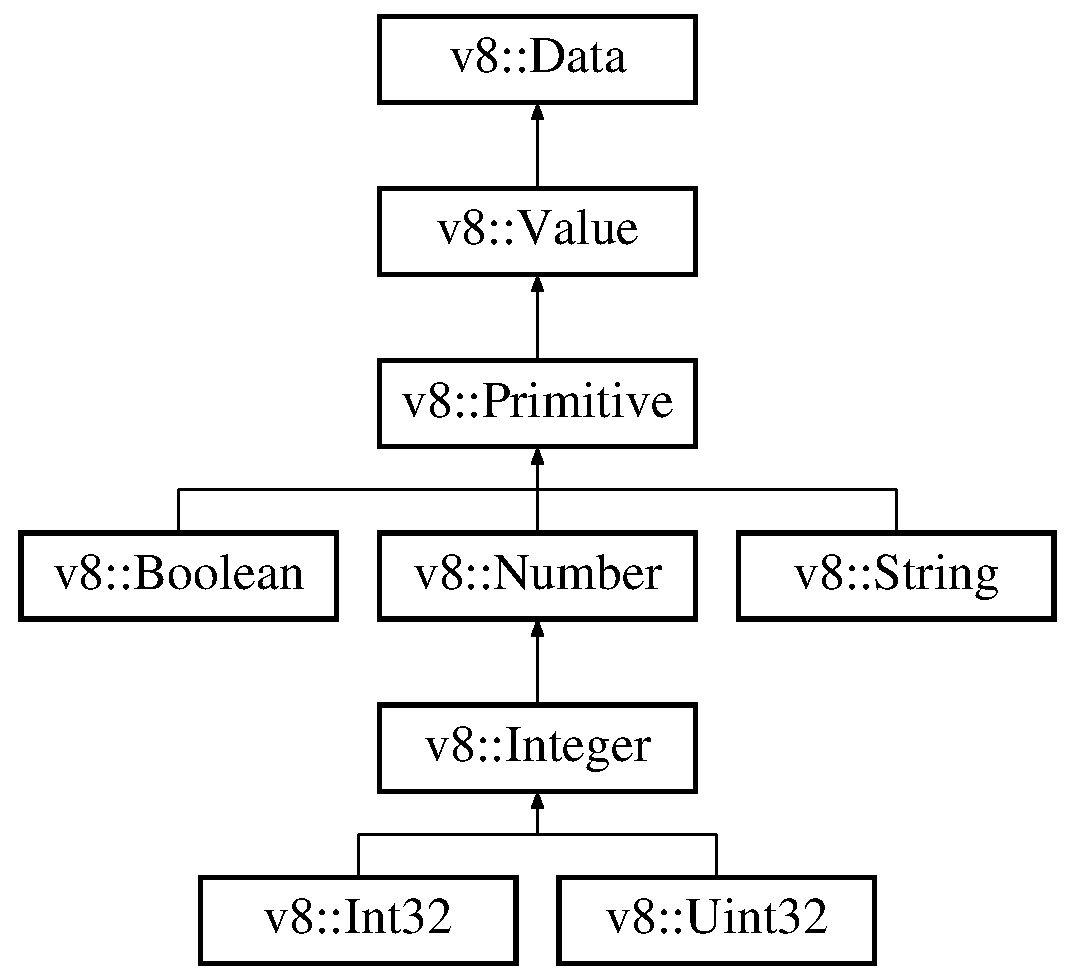
\includegraphics[height=6.000000cm]{classv8_1_1_primitive}
\end{center}
\end{figure}
\subsection*{Additional Inherited Members}


\subsection{Detailed Description}
The superclass of primitive values. See E\+C\+M\+A-\/262 4.\+3.\+2. 

The documentation for this class was generated from the following file\+:\begin{DoxyCompactItemize}
\item 
deps/v8/include/v8.\+h\end{DoxyCompactItemize}

\hypertarget{classv8_1_1_reg_exp}{}\section{v8\+:\+:Reg\+Exp Class Reference}
\label{classv8_1_1_reg_exp}\index{v8\+::\+Reg\+Exp@{v8\+::\+Reg\+Exp}}


{\ttfamily \#include $<$v8.\+h$>$}

Inheritance diagram for v8\+:\+:Reg\+Exp\+:\begin{figure}[H]
\begin{center}
\leavevmode
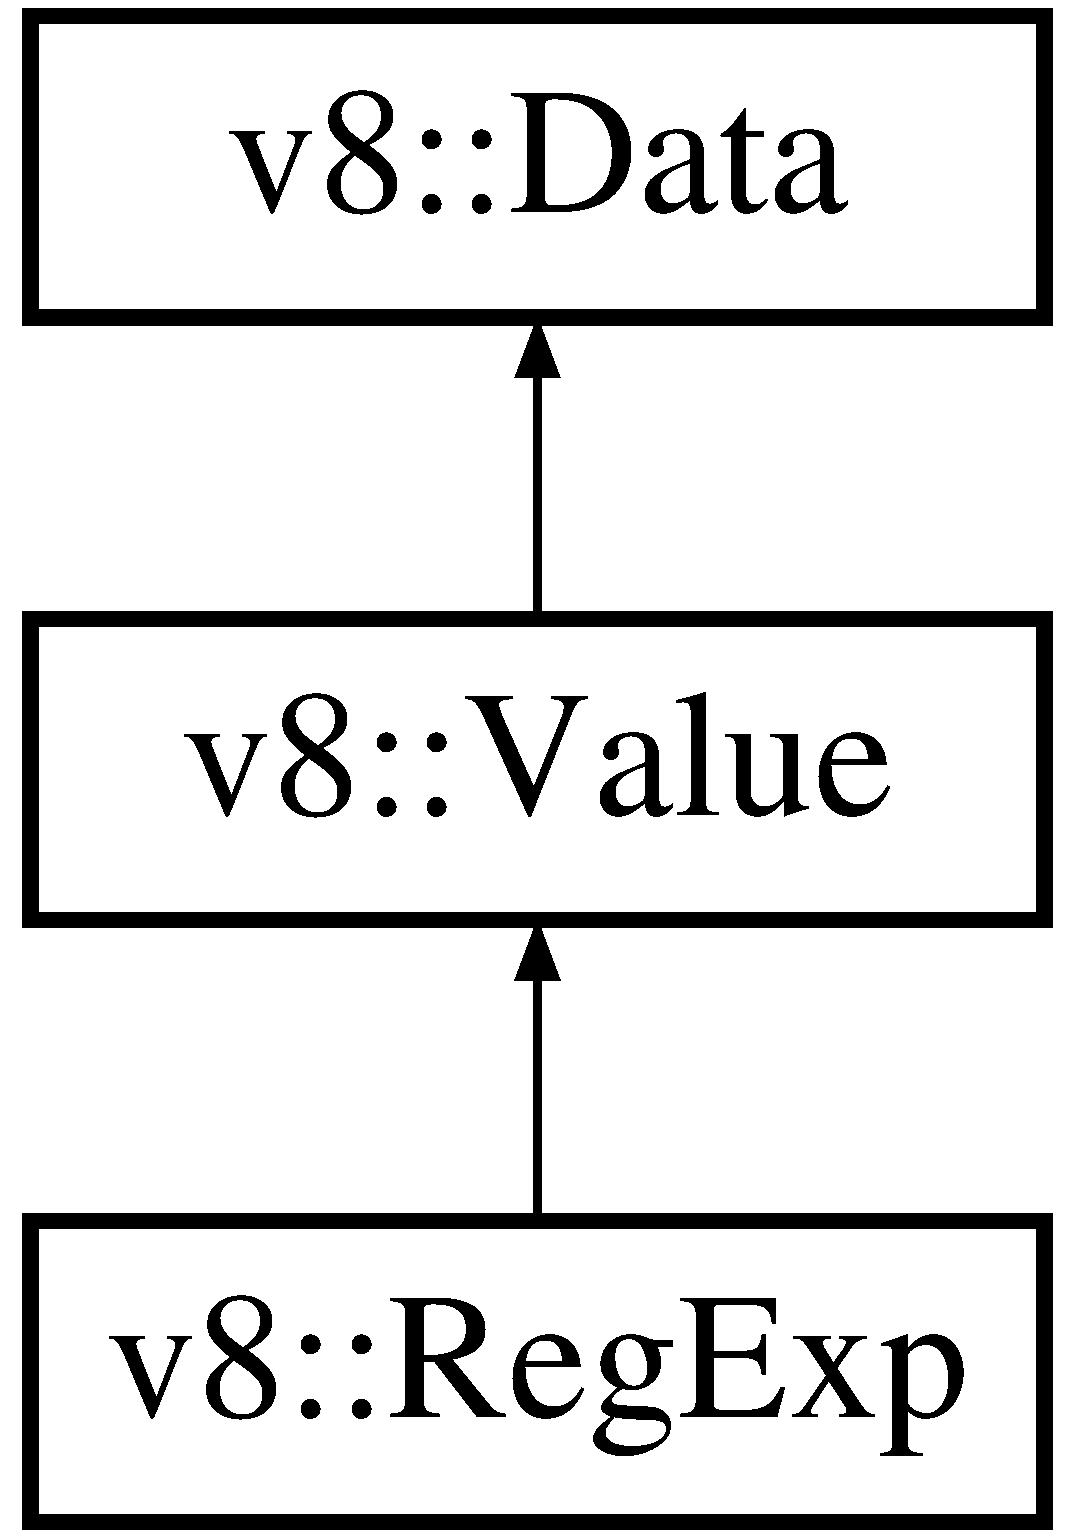
\includegraphics[height=4.000000cm]{classv8_1_1_reg_exp}
\end{center}
\end{figure}
\subsection*{Public Types}
\begin{DoxyCompactItemize}
\item 
enum \hyperlink{classv8_1_1_reg_exp_aa4718a5c1f18472aff3bf51ed694fc5a}{Flags} \{ {\bfseries k\+None} = 0, 
{\bfseries k\+Global} = 1, 
{\bfseries k\+Ignore\+Case} = 2, 
{\bfseries k\+Multiline} = 4
 \}
\end{DoxyCompactItemize}
\subsection*{Public Member Functions}
\begin{DoxyCompactItemize}
\item 
V8\+E\+X\+P\+O\+R\+T \hyperlink{classv8_1_1_local}{Local}$<$ \hyperlink{classv8_1_1_string}{String} $>$ \hyperlink{classv8_1_1_reg_exp_aaaaa82b4490fe1eb0d470370293e770e}{Get\+Source} () const 
\item 
V8\+E\+X\+P\+O\+R\+T \hyperlink{classv8_1_1_reg_exp_aa4718a5c1f18472aff3bf51ed694fc5a}{Flags} \hyperlink{classv8_1_1_reg_exp_a02c7a85155ff5d2883ffc699e36ada4c}{Get\+Flags} () const 
\item 
\hypertarget{classv8_1_1_reg_exp_ad65e1ae3851100b0590b47145000976a}{}{\bfseries V8\+\_\+\+I\+N\+L\+I\+N\+E} (static \hyperlink{classv8_1_1_reg_exp}{Reg\+Exp} $\ast$Cast(\hyperlink{classv8_1_1_value}{v8\+::\+Value} $\ast$obj))\label{classv8_1_1_reg_exp_ad65e1ae3851100b0590b47145000976a}

\end{DoxyCompactItemize}
\subsection*{Static Public Member Functions}
\begin{DoxyCompactItemize}
\item 
static V8\+E\+X\+P\+O\+R\+T \hyperlink{classv8_1_1_local}{Local}$<$ \hyperlink{classv8_1_1_reg_exp}{Reg\+Exp} $>$ \hyperlink{classv8_1_1_reg_exp_a27390ac15b8b52057927e8c78491aacb}{New} (\hyperlink{classv8_1_1_handle}{Handle}$<$ \hyperlink{classv8_1_1_string}{String} $>$ pattern, \hyperlink{classv8_1_1_reg_exp_aa4718a5c1f18472aff3bf51ed694fc5a}{Flags} flags)
\end{DoxyCompactItemize}


\subsection{Detailed Description}
An instance of the built-\/in \hyperlink{classv8_1_1_reg_exp}{Reg\+Exp} constructor (E\+C\+M\+A-\/262, 15.\+10). 

\subsection{Member Enumeration Documentation}
\hypertarget{classv8_1_1_reg_exp_aa4718a5c1f18472aff3bf51ed694fc5a}{}\index{v8\+::\+Reg\+Exp@{v8\+::\+Reg\+Exp}!Flags@{Flags}}
\index{Flags@{Flags}!v8\+::\+Reg\+Exp@{v8\+::\+Reg\+Exp}}
\subsubsection[{Flags}]{\setlength{\rightskip}{0pt plus 5cm}enum {\bf v8\+::\+Reg\+Exp\+::\+Flags}}\label{classv8_1_1_reg_exp_aa4718a5c1f18472aff3bf51ed694fc5a}
Regular expression flag bits. They can be or\textquotesingle{}ed to enable a set of flags. 

\subsection{Member Function Documentation}
\hypertarget{classv8_1_1_reg_exp_a02c7a85155ff5d2883ffc699e36ada4c}{}\index{v8\+::\+Reg\+Exp@{v8\+::\+Reg\+Exp}!Get\+Flags@{Get\+Flags}}
\index{Get\+Flags@{Get\+Flags}!v8\+::\+Reg\+Exp@{v8\+::\+Reg\+Exp}}
\subsubsection[{Get\+Flags}]{\setlength{\rightskip}{0pt plus 5cm}V8\+E\+X\+P\+O\+R\+T {\bf Flags} v8\+::\+Reg\+Exp\+::\+Get\+Flags (
\begin{DoxyParamCaption}
{}
\end{DoxyParamCaption}
) const}\label{classv8_1_1_reg_exp_a02c7a85155ff5d2883ffc699e36ada4c}
Returns the flags bit field. \hypertarget{classv8_1_1_reg_exp_aaaaa82b4490fe1eb0d470370293e770e}{}\index{v8\+::\+Reg\+Exp@{v8\+::\+Reg\+Exp}!Get\+Source@{Get\+Source}}
\index{Get\+Source@{Get\+Source}!v8\+::\+Reg\+Exp@{v8\+::\+Reg\+Exp}}
\subsubsection[{Get\+Source}]{\setlength{\rightskip}{0pt plus 5cm}V8\+E\+X\+P\+O\+R\+T {\bf Local}$<${\bf String}$>$ v8\+::\+Reg\+Exp\+::\+Get\+Source (
\begin{DoxyParamCaption}
{}
\end{DoxyParamCaption}
) const}\label{classv8_1_1_reg_exp_aaaaa82b4490fe1eb0d470370293e770e}
Returns the value of the source property\+: a string representing the regular expression. \hypertarget{classv8_1_1_reg_exp_a27390ac15b8b52057927e8c78491aacb}{}\index{v8\+::\+Reg\+Exp@{v8\+::\+Reg\+Exp}!New@{New}}
\index{New@{New}!v8\+::\+Reg\+Exp@{v8\+::\+Reg\+Exp}}
\subsubsection[{New}]{\setlength{\rightskip}{0pt plus 5cm}static V8\+E\+X\+P\+O\+R\+T {\bf Local}$<${\bf Reg\+Exp}$>$ v8\+::\+Reg\+Exp\+::\+New (
\begin{DoxyParamCaption}
\item[{{\bf Handle}$<$ {\bf String} $>$}]{pattern, }
\item[{{\bf Flags}}]{flags}
\end{DoxyParamCaption}
)\hspace{0.3cm}{\ttfamily [static]}}\label{classv8_1_1_reg_exp_a27390ac15b8b52057927e8c78491aacb}
Creates a regular expression from the given pattern string and the flags bit field. May throw a Java\+Script exception as described in E\+C\+M\+A-\/262, 15.\+10.\+4.\+1.

For example, \hyperlink{classv8_1_1_reg_exp_a27390ac15b8b52057927e8c78491aacb}{Reg\+Exp\+::\+New}(\hyperlink{classv8_1_1_string_af0f9c44d85056bd575c01e8be7cc1b01}{v8\+::\+String\+::\+New}(\char`\"{}foo\char`\"{}), static\+\_\+cast$<$\+Reg\+Exp\+::\+Flags$>$(k\+Global $\vert$ k\+Multiline)) is equivalent to evaluating \char`\"{}/foo/gm\char`\"{}. 

The documentation for this class was generated from the following file\+:\begin{DoxyCompactItemize}
\item 
deps/v8/include/v8.\+h\end{DoxyCompactItemize}

\hypertarget{classv8_1_1_resource_constraints}{}\section{v8\+:\+:Resource\+Constraints Class Reference}
\label{classv8_1_1_resource_constraints}\index{v8\+::\+Resource\+Constraints@{v8\+::\+Resource\+Constraints}}


{\ttfamily \#include $<$v8.\+h$>$}

\subsection*{Public Member Functions}
\begin{DoxyCompactItemize}
\item 
void \hyperlink{classv8_1_1_resource_constraints_aeeaaee4017e8d5f8f0439af2af2ed3a5}{Configure\+Defaults} (uint64\+\_\+t physical\+\_\+memory, uint64\+\_\+t virtual\+\_\+memory\+\_\+limit)
\item 
\hypertarget{classv8_1_1_resource_constraints_a9cdff07ac0633cd33eddd4e58cbfa3a9}{}{\bfseries V8\+\_\+\+D\+E\+P\+R\+E\+C\+A\+T\+E\+D} (\char`\"{}Use two-\/args version instead\char`\"{}, void \hyperlink{classv8_1_1_resource_constraints_aeeaaee4017e8d5f8f0439af2af2ed3a5}{Configure\+Defaults}(uint64\+\_\+t physical\+\_\+memory, uint64\+\_\+t virtual\+\_\+memory\+\_\+limit, uint32\+\_\+t number\+\_\+of\+\_\+processors))\label{classv8_1_1_resource_constraints_a9cdff07ac0633cd33eddd4e58cbfa3a9}

\item 
\hypertarget{classv8_1_1_resource_constraints_aeeecbbdb2c7880bf74d5d7fb9bbc52b3}{}int {\bfseries max\+\_\+semi\+\_\+space\+\_\+size} () const \label{classv8_1_1_resource_constraints_aeeecbbdb2c7880bf74d5d7fb9bbc52b3}

\item 
\hypertarget{classv8_1_1_resource_constraints_ac83efbf72458c872009f66019352409e}{}void {\bfseries set\+\_\+max\+\_\+semi\+\_\+space\+\_\+size} (int value)\label{classv8_1_1_resource_constraints_ac83efbf72458c872009f66019352409e}

\item 
\hypertarget{classv8_1_1_resource_constraints_a72840efdbcfc7bb287c6aea38d0b07b9}{}int {\bfseries max\+\_\+old\+\_\+space\+\_\+size} () const \label{classv8_1_1_resource_constraints_a72840efdbcfc7bb287c6aea38d0b07b9}

\item 
\hypertarget{classv8_1_1_resource_constraints_aa764be7c76b4baa3fce7a54c3777b5e9}{}void {\bfseries set\+\_\+max\+\_\+old\+\_\+space\+\_\+size} (int value)\label{classv8_1_1_resource_constraints_aa764be7c76b4baa3fce7a54c3777b5e9}

\item 
\hypertarget{classv8_1_1_resource_constraints_a037777e608ed1c22fe294ecef5722036}{}int {\bfseries max\+\_\+executable\+\_\+size} () const \label{classv8_1_1_resource_constraints_a037777e608ed1c22fe294ecef5722036}

\item 
\hypertarget{classv8_1_1_resource_constraints_a37d1b38672e9844c567823a119dcd557}{}void {\bfseries set\+\_\+max\+\_\+executable\+\_\+size} (int value)\label{classv8_1_1_resource_constraints_a37d1b38672e9844c567823a119dcd557}

\item 
\hypertarget{classv8_1_1_resource_constraints_aafc4a94f2eeb0684e7a50f355eb4d06d}{}uint32\+\_\+t $\ast$ {\bfseries stack\+\_\+limit} () const \label{classv8_1_1_resource_constraints_aafc4a94f2eeb0684e7a50f355eb4d06d}

\item 
\hypertarget{classv8_1_1_resource_constraints_a26ed3e89985a4afe34e84509fb093cf1}{}void {\bfseries set\+\_\+stack\+\_\+limit} (uint32\+\_\+t $\ast$value)\label{classv8_1_1_resource_constraints_a26ed3e89985a4afe34e84509fb093cf1}

\item 
\hypertarget{classv8_1_1_resource_constraints_ac9f4b9010ed635944cffee59f4f22795}{}{\bfseries V8\+\_\+\+D\+E\+P\+R\+E\+C\+A\+T\+E\+D} (\char`\"{}Unused, will be removed\char`\"{}, int max\+\_\+available\+\_\+threads() const)\label{classv8_1_1_resource_constraints_ac9f4b9010ed635944cffee59f4f22795}

\item 
\hypertarget{classv8_1_1_resource_constraints_a5a5c9962c1376dd99511fea06659abdb}{}{\bfseries V8\+\_\+\+D\+E\+P\+R\+E\+C\+A\+T\+E\+D} (\char`\"{}Unused, will be removed\char`\"{}, void set\+\_\+max\+\_\+available\+\_\+threads(int value))\label{classv8_1_1_resource_constraints_a5a5c9962c1376dd99511fea06659abdb}

\item 
\hypertarget{classv8_1_1_resource_constraints_a8dd511917ad17bf2185d574b0c7e4186}{}size\+\_\+t {\bfseries code\+\_\+range\+\_\+size} () const \label{classv8_1_1_resource_constraints_a8dd511917ad17bf2185d574b0c7e4186}

\item 
\hypertarget{classv8_1_1_resource_constraints_af887bf453b41b79eb174e5eeee0f1db2}{}void {\bfseries set\+\_\+code\+\_\+range\+\_\+size} (size\+\_\+t value)\label{classv8_1_1_resource_constraints_af887bf453b41b79eb174e5eeee0f1db2}

\end{DoxyCompactItemize}


\subsection{Detailed Description}
A set of constraints that specifies the limits of the runtime\textquotesingle{}s memory use. You must set the heap size before initializing the V\+M -\/ the size cannot be adjusted after the V\+M is initialized.

If you are using threads then you should hold the V8\+::\+Locker lock while setting the stack limit and you must set a non-\/default stack limit separately for each thread. 

\subsection{Member Function Documentation}
\hypertarget{classv8_1_1_resource_constraints_aeeaaee4017e8d5f8f0439af2af2ed3a5}{}\index{v8\+::\+Resource\+Constraints@{v8\+::\+Resource\+Constraints}!Configure\+Defaults@{Configure\+Defaults}}
\index{Configure\+Defaults@{Configure\+Defaults}!v8\+::\+Resource\+Constraints@{v8\+::\+Resource\+Constraints}}
\subsubsection[{Configure\+Defaults}]{\setlength{\rightskip}{0pt plus 5cm}void v8\+::\+Resource\+Constraints\+::\+Configure\+Defaults (
\begin{DoxyParamCaption}
\item[{uint64\+\_\+t}]{physical\+\_\+memory, }
\item[{uint64\+\_\+t}]{virtual\+\_\+memory\+\_\+limit}
\end{DoxyParamCaption}
)}\label{classv8_1_1_resource_constraints_aeeaaee4017e8d5f8f0439af2af2ed3a5}
Configures the constraints with reasonable default values based on the capabilities of the current device the V\+M is running on.


\begin{DoxyParams}{Parameters}
{\em physical\+\_\+memory} & The total amount of physical memory on the current device, in bytes. \\
\hline
{\em virtual\+\_\+memory\+\_\+limit} & The amount of virtual memory on the current device, in bytes, or zero, if there is no limit. \\
\hline
\end{DoxyParams}


The documentation for this class was generated from the following file\+:\begin{DoxyCompactItemize}
\item 
deps/v8/include/v8.\+h\end{DoxyCompactItemize}

\hypertarget{classv8_1_1_context_1_1_scope}{}\section{v8\+:\+:Context\+:\+:Scope Class Reference}
\label{classv8_1_1_context_1_1_scope}\index{v8\+::\+Context\+::\+Scope@{v8\+::\+Context\+::\+Scope}}


{\ttfamily \#include $<$v8.\+h$>$}

\subsection*{Public Member Functions}
\begin{DoxyCompactItemize}
\item 
\hypertarget{classv8_1_1_context_1_1_scope_a193358558d5c1f62b6900b9d8de6807e}{}{\bfseries V8\+\_\+\+I\+N\+L\+I\+N\+E} (\hyperlink{classv8_1_1_context_1_1_scope}{Scope}(\hyperlink{classv8_1_1_handle}{Handle}$<$ \hyperlink{classv8_1_1_context}{Context} $>$ context))\label{classv8_1_1_context_1_1_scope_a193358558d5c1f62b6900b9d8de6807e}

\item 
\hypertarget{classv8_1_1_context_1_1_scope_aa1f9dad2490075b07fa71621b5112bf8}{}{\bfseries V8\+\_\+\+I\+N\+L\+I\+N\+E} (\hyperlink{classv8_1_1_context_1_1_scope}{Scope}(\hyperlink{classv8_1_1_isolate}{Isolate} $\ast$isolate, \hyperlink{classv8_1_1_persistent}{Persistent}$<$ \hyperlink{classv8_1_1_context}{Context} $>$ \&context))\label{classv8_1_1_context_1_1_scope_aa1f9dad2490075b07fa71621b5112bf8}

\item 
\hypertarget{classv8_1_1_context_1_1_scope_ac2a1c73e596c9f2f9921bd9d629ee9d2}{}{\bfseries V8\+\_\+\+I\+N\+L\+I\+N\+E} ($\sim$\hyperlink{classv8_1_1_context_1_1_scope}{Scope}())\label{classv8_1_1_context_1_1_scope_ac2a1c73e596c9f2f9921bd9d629ee9d2}

\end{DoxyCompactItemize}


\subsection{Detailed Description}
Stack-\/allocated class which sets the execution context for all operations executed within a local scope. 

The documentation for this class was generated from the following file\+:\begin{DoxyCompactItemize}
\item 
deps/v8/include/v8.\+h\end{DoxyCompactItemize}

\hypertarget{classv8_1_1_script}{}\section{v8\+:\+:Script Class Reference}
\label{classv8_1_1_script}\index{v8\+::\+Script@{v8\+::\+Script}}


{\ttfamily \#include $<$v8.\+h$>$}

\subsection*{Public Member Functions}
\begin{DoxyCompactItemize}
\item 
\hyperlink{classv8_1_1_local}{Local}$<$ \hyperlink{classv8_1_1_value}{Value} $>$ \hyperlink{classv8_1_1_script_a5f43b29d40bd51ebad2cc275ba3898a1}{Run} ()
\item 
\hyperlink{classv8_1_1_local}{Local}$<$ \hyperlink{classv8_1_1_unbound_script}{Unbound\+Script} $>$ \hyperlink{classv8_1_1_script_afac25cad452a61897c375c2b881e2070}{Get\+Unbound\+Script} ()
\item 
\hypertarget{classv8_1_1_script_a0b781b6966adf4beb558eea17bfd998c}{}{\bfseries V8\+\_\+\+D\+E\+P\+R\+E\+C\+A\+T\+E\+D} (\char`\"{}Use \hyperlink{classv8_1_1_script_afac25cad452a61897c375c2b881e2070}{Get\+Unbound\+Script}()-\/$>$Get\+Id()\char`\"{}, int Get\+Id())\label{classv8_1_1_script_a0b781b6966adf4beb558eea17bfd998c}

\end{DoxyCompactItemize}
\subsection*{Static Public Member Functions}
\begin{DoxyCompactItemize}
\item 
static \hyperlink{classv8_1_1_local}{Local}$<$ \hyperlink{classv8_1_1_script}{Script} $>$ \hyperlink{classv8_1_1_script_a78500f4a95d75ffd0253f72a6db750b0}{Compile} (\hyperlink{classv8_1_1_handle}{Handle}$<$ \hyperlink{classv8_1_1_string}{String} $>$ source, \hyperlink{classv8_1_1_script_origin}{Script\+Origin} $\ast$origin=N\+U\+L\+L)
\item 
\hypertarget{classv8_1_1_script_ae420c65d6315f3ef8e83e79c17231f4e}{}static \hyperlink{classv8_1_1_local}{Local}$<$ \hyperlink{classv8_1_1_script}{Script} $>$ {\bfseries Compile} (\hyperlink{classv8_1_1_handle}{Handle}$<$ \hyperlink{classv8_1_1_string}{String} $>$ source, \hyperlink{classv8_1_1_handle}{Handle}$<$ \hyperlink{classv8_1_1_string}{String} $>$ file\+\_\+name)\label{classv8_1_1_script_ae420c65d6315f3ef8e83e79c17231f4e}

\end{DoxyCompactItemize}


\subsection{Detailed Description}
A compiled Java\+Script script, tied to a \hyperlink{classv8_1_1_context}{Context} which was active when the script was compiled. 

\subsection{Member Function Documentation}
\hypertarget{classv8_1_1_script_a78500f4a95d75ffd0253f72a6db750b0}{}\index{v8\+::\+Script@{v8\+::\+Script}!Compile@{Compile}}
\index{Compile@{Compile}!v8\+::\+Script@{v8\+::\+Script}}
\subsubsection[{Compile}]{\setlength{\rightskip}{0pt plus 5cm}static {\bf Local}$<${\bf Script}$>$ v8\+::\+Script\+::\+Compile (
\begin{DoxyParamCaption}
\item[{{\bf Handle}$<$ {\bf String} $>$}]{source, }
\item[{{\bf Script\+Origin} $\ast$}]{origin = {\ttfamily NULL}}
\end{DoxyParamCaption}
)\hspace{0.3cm}{\ttfamily [static]}}\label{classv8_1_1_script_a78500f4a95d75ffd0253f72a6db750b0}
A shorthand for \hyperlink{classv8_1_1_script_compiler_a4cef8b34c2744f6508a9ce53182c19bf}{Script\+Compiler\+::\+Compile()}. \hypertarget{classv8_1_1_script_afac25cad452a61897c375c2b881e2070}{}\index{v8\+::\+Script@{v8\+::\+Script}!Get\+Unbound\+Script@{Get\+Unbound\+Script}}
\index{Get\+Unbound\+Script@{Get\+Unbound\+Script}!v8\+::\+Script@{v8\+::\+Script}}
\subsubsection[{Get\+Unbound\+Script}]{\setlength{\rightskip}{0pt plus 5cm}{\bf Local}$<${\bf Unbound\+Script}$>$ v8\+::\+Script\+::\+Get\+Unbound\+Script (
\begin{DoxyParamCaption}
{}
\end{DoxyParamCaption}
)}\label{classv8_1_1_script_afac25cad452a61897c375c2b881e2070}
Returns the corresponding context-\/unbound script. \hypertarget{classv8_1_1_script_a5f43b29d40bd51ebad2cc275ba3898a1}{}\index{v8\+::\+Script@{v8\+::\+Script}!Run@{Run}}
\index{Run@{Run}!v8\+::\+Script@{v8\+::\+Script}}
\subsubsection[{Run}]{\setlength{\rightskip}{0pt plus 5cm}{\bf Local}$<${\bf Value}$>$ v8\+::\+Script\+::\+Run (
\begin{DoxyParamCaption}
{}
\end{DoxyParamCaption}
)}\label{classv8_1_1_script_a5f43b29d40bd51ebad2cc275ba3898a1}
Runs the script returning the resulting value. It will be run in the context in which it was created (Script\+Compiler\+::\+Compile\+Bound or Unbound\+Script\+::\+Bind\+To\+Global\+Context()). 

The documentation for this class was generated from the following file\+:\begin{DoxyCompactItemize}
\item 
deps/v8/include/v8.\+h\end{DoxyCompactItemize}

\hypertarget{classv8_1_1_script_data}{}\section{v8\+:\+:Script\+Data Class Reference}
\label{classv8_1_1_script_data}\index{v8\+::\+Script\+Data@{v8\+::\+Script\+Data}}


{\ttfamily \#include $<$v8.\+h$>$}

\subsection*{Public Member Functions}
\begin{DoxyCompactItemize}
\item 
virtual int \hyperlink{classv8_1_1_script_data_a6aa1007dfe6b09a5e59443bb1afff0b9}{Length} ()=0
\item 
virtual const char $\ast$ \hyperlink{classv8_1_1_script_data_aae01a4e977988fa8338d11d87b572cfa}{Data} ()=0
\item 
virtual bool \hyperlink{classv8_1_1_script_data_ab5cea77b299b7dd73b7024fb114fd7e4}{Has\+Error} ()=0
\end{DoxyCompactItemize}
\subsection*{Static Public Member Functions}
\begin{DoxyCompactItemize}
\item 
static \hyperlink{classv8_1_1_script_data}{Script\+Data} $\ast$ \hyperlink{classv8_1_1_script_data_a0ae4b2c878a42cfea7afcc8898e24cae}{Pre\+Compile} (\hyperlink{classv8_1_1_isolate}{Isolate} $\ast$isolate, const char $\ast$input, int length)
\item 
static \hyperlink{classv8_1_1_script_data}{Script\+Data} $\ast$ \hyperlink{classv8_1_1_script_data_ad1e46f2a1e84ae151b295f3c74c71787}{Pre\+Compile} (\hyperlink{classv8_1_1_handle}{Handle}$<$ \hyperlink{classv8_1_1_string}{String} $>$ source)
\item 
static \hyperlink{classv8_1_1_script_data}{Script\+Data} $\ast$ \hyperlink{classv8_1_1_script_data_a642fc06a9615387f9ac80f264758cc70}{New} (const char $\ast$data, int length)
\end{DoxyCompactItemize}


\subsection{Detailed Description}
Pre-\/compilation data that can be associated with a script. This data can be calculated for a script in advance of actually compiling it, and can be stored between compilations. When script data is given to the compile method compilation will be faster. 

\subsection{Member Function Documentation}
\hypertarget{classv8_1_1_script_data_aae01a4e977988fa8338d11d87b572cfa}{}\index{v8\+::\+Script\+Data@{v8\+::\+Script\+Data}!Data@{Data}}
\index{Data@{Data}!v8\+::\+Script\+Data@{v8\+::\+Script\+Data}}
\subsubsection[{Data}]{\setlength{\rightskip}{0pt plus 5cm}virtual const char$\ast$ v8\+::\+Script\+Data\+::\+Data (
\begin{DoxyParamCaption}
{}
\end{DoxyParamCaption}
)\hspace{0.3cm}{\ttfamily [pure virtual]}}\label{classv8_1_1_script_data_aae01a4e977988fa8338d11d87b572cfa}
Returns a serialized representation of this \hyperlink{classv8_1_1_script_data}{Script\+Data} that can later be passed to \hyperlink{classv8_1_1_script_data_a642fc06a9615387f9ac80f264758cc70}{New()}. N\+O\+T\+E\+: Serialized data is platform-\/dependent. \hypertarget{classv8_1_1_script_data_ab5cea77b299b7dd73b7024fb114fd7e4}{}\index{v8\+::\+Script\+Data@{v8\+::\+Script\+Data}!Has\+Error@{Has\+Error}}
\index{Has\+Error@{Has\+Error}!v8\+::\+Script\+Data@{v8\+::\+Script\+Data}}
\subsubsection[{Has\+Error}]{\setlength{\rightskip}{0pt plus 5cm}virtual bool v8\+::\+Script\+Data\+::\+Has\+Error (
\begin{DoxyParamCaption}
{}
\end{DoxyParamCaption}
)\hspace{0.3cm}{\ttfamily [pure virtual]}}\label{classv8_1_1_script_data_ab5cea77b299b7dd73b7024fb114fd7e4}
Returns true if the source code could not be parsed. \hypertarget{classv8_1_1_script_data_a6aa1007dfe6b09a5e59443bb1afff0b9}{}\index{v8\+::\+Script\+Data@{v8\+::\+Script\+Data}!Length@{Length}}
\index{Length@{Length}!v8\+::\+Script\+Data@{v8\+::\+Script\+Data}}
\subsubsection[{Length}]{\setlength{\rightskip}{0pt plus 5cm}virtual int v8\+::\+Script\+Data\+::\+Length (
\begin{DoxyParamCaption}
{}
\end{DoxyParamCaption}
)\hspace{0.3cm}{\ttfamily [pure virtual]}}\label{classv8_1_1_script_data_a6aa1007dfe6b09a5e59443bb1afff0b9}
Returns the length of \hyperlink{classv8_1_1_script_data_aae01a4e977988fa8338d11d87b572cfa}{Data()}. \hypertarget{classv8_1_1_script_data_a642fc06a9615387f9ac80f264758cc70}{}\index{v8\+::\+Script\+Data@{v8\+::\+Script\+Data}!New@{New}}
\index{New@{New}!v8\+::\+Script\+Data@{v8\+::\+Script\+Data}}
\subsubsection[{New}]{\setlength{\rightskip}{0pt plus 5cm}static {\bf Script\+Data}$\ast$ v8\+::\+Script\+Data\+::\+New (
\begin{DoxyParamCaption}
\item[{const char $\ast$}]{data, }
\item[{int}]{length}
\end{DoxyParamCaption}
)\hspace{0.3cm}{\ttfamily [static]}}\label{classv8_1_1_script_data_a642fc06a9615387f9ac80f264758cc70}
Load previous pre-\/compilation data.


\begin{DoxyParams}{Parameters}
{\em data} & Pointer to data returned by a call to \hyperlink{classv8_1_1_script_data_aae01a4e977988fa8338d11d87b572cfa}{Data()} of a previous \hyperlink{classv8_1_1_script_data}{Script\+Data}. Ownership is not transferred. \\
\hline
{\em length} & Length of data. \\
\hline
\end{DoxyParams}
\hypertarget{classv8_1_1_script_data_a0ae4b2c878a42cfea7afcc8898e24cae}{}\index{v8\+::\+Script\+Data@{v8\+::\+Script\+Data}!Pre\+Compile@{Pre\+Compile}}
\index{Pre\+Compile@{Pre\+Compile}!v8\+::\+Script\+Data@{v8\+::\+Script\+Data}}
\subsubsection[{Pre\+Compile}]{\setlength{\rightskip}{0pt plus 5cm}static {\bf Script\+Data}$\ast$ v8\+::\+Script\+Data\+::\+Pre\+Compile (
\begin{DoxyParamCaption}
\item[{{\bf Isolate} $\ast$}]{isolate, }
\item[{const char $\ast$}]{input, }
\item[{int}]{length}
\end{DoxyParamCaption}
)\hspace{0.3cm}{\ttfamily [static]}}\label{classv8_1_1_script_data_a0ae4b2c878a42cfea7afcc8898e24cae}
Pre-\/compiles the specified script (context-\/independent).


\begin{DoxyParams}{Parameters}
{\em input} & Pointer to U\+T\+F-\/8 script source code. \\
\hline
{\em length} & Length of U\+T\+F-\/8 script source code. \\
\hline
\end{DoxyParams}
\hypertarget{classv8_1_1_script_data_ad1e46f2a1e84ae151b295f3c74c71787}{}\index{v8\+::\+Script\+Data@{v8\+::\+Script\+Data}!Pre\+Compile@{Pre\+Compile}}
\index{Pre\+Compile@{Pre\+Compile}!v8\+::\+Script\+Data@{v8\+::\+Script\+Data}}
\subsubsection[{Pre\+Compile}]{\setlength{\rightskip}{0pt plus 5cm}static {\bf Script\+Data}$\ast$ v8\+::\+Script\+Data\+::\+Pre\+Compile (
\begin{DoxyParamCaption}
\item[{{\bf Handle}$<$ {\bf String} $>$}]{source}
\end{DoxyParamCaption}
)\hspace{0.3cm}{\ttfamily [static]}}\label{classv8_1_1_script_data_ad1e46f2a1e84ae151b295f3c74c71787}
Pre-\/compiles the specified script (context-\/independent).

N\+O\+T\+E\+: Pre-\/compilation using this method cannot happen on another thread without using Lockers.


\begin{DoxyParams}{Parameters}
{\em source} & \hyperlink{classv8_1_1_script}{Script} source code. \\
\hline
\end{DoxyParams}


The documentation for this class was generated from the following file\+:\begin{DoxyCompactItemize}
\item 
deps/v8/include/v8.\+h\end{DoxyCompactItemize}

\hypertarget{classv8_1_1_script_origin}{}\section{v8\+:\+:Script\+Origin Class Reference}
\label{classv8_1_1_script_origin}\index{v8\+::\+Script\+Origin@{v8\+::\+Script\+Origin}}


{\ttfamily \#include $<$v8.\+h$>$}

\subsection*{Public Member Functions}
\begin{DoxyCompactItemize}
\item 
\hypertarget{classv8_1_1_script_origin_a59a6e8e17f7206e907d2c46c7c962eab}{}V8\+\_\+\+I\+N\+L\+I\+N\+E {\bfseries Script\+Origin} (\hyperlink{classv8_1_1_handle}{Handle}$<$ \hyperlink{classv8_1_1_value}{Value} $>$ resource\+\_\+name, \hyperlink{classv8_1_1_handle}{Handle}$<$ \hyperlink{classv8_1_1_integer}{Integer} $>$ resource\+\_\+line\+\_\+offset=\hyperlink{classv8_1_1_handle}{Handle}$<$ \hyperlink{classv8_1_1_integer}{Integer} $>$(), \hyperlink{classv8_1_1_handle}{Handle}$<$ \hyperlink{classv8_1_1_integer}{Integer} $>$ resource\+\_\+column\+\_\+offset=\hyperlink{classv8_1_1_handle}{Handle}$<$ \hyperlink{classv8_1_1_integer}{Integer} $>$(), \hyperlink{classv8_1_1_handle}{Handle}$<$ \hyperlink{classv8_1_1_boolean}{Boolean} $>$ resource\+\_\+is\+\_\+shared\+\_\+cross\+\_\+origin=\hyperlink{classv8_1_1_handle}{Handle}$<$ \hyperlink{classv8_1_1_boolean}{Boolean} $>$())\label{classv8_1_1_script_origin_a59a6e8e17f7206e907d2c46c7c962eab}

\item 
\hypertarget{classv8_1_1_script_origin_a289502d71720ca10e53b4a32d9226f58}{}V8\+\_\+\+I\+N\+L\+I\+N\+E \hyperlink{classv8_1_1_handle}{Handle}$<$ \hyperlink{classv8_1_1_value}{Value} $>$ {\bfseries Resource\+Name} () const \label{classv8_1_1_script_origin_a289502d71720ca10e53b4a32d9226f58}

\item 
\hypertarget{classv8_1_1_script_origin_a0735178b8afef9169a3481cf6cd7c557}{}V8\+\_\+\+I\+N\+L\+I\+N\+E \hyperlink{classv8_1_1_handle}{Handle}$<$ \hyperlink{classv8_1_1_integer}{Integer} $>$ {\bfseries Resource\+Line\+Offset} () const \label{classv8_1_1_script_origin_a0735178b8afef9169a3481cf6cd7c557}

\item 
\hypertarget{classv8_1_1_script_origin_a6d1b4cb1be2b6589151a029974cd1a60}{}V8\+\_\+\+I\+N\+L\+I\+N\+E \hyperlink{classv8_1_1_handle}{Handle}$<$ \hyperlink{classv8_1_1_integer}{Integer} $>$ {\bfseries Resource\+Column\+Offset} () const \label{classv8_1_1_script_origin_a6d1b4cb1be2b6589151a029974cd1a60}

\item 
\hypertarget{classv8_1_1_script_origin_a632d2d30405d42512af609861e486bf2}{}V8\+\_\+\+I\+N\+L\+I\+N\+E \hyperlink{classv8_1_1_handle}{Handle}$<$ \hyperlink{classv8_1_1_boolean}{Boolean} $>$ {\bfseries Resource\+Is\+Shared\+Cross\+Origin} () const \label{classv8_1_1_script_origin_a632d2d30405d42512af609861e486bf2}

\end{DoxyCompactItemize}


\subsection{Detailed Description}
The origin, within a file, of a script. 

The documentation for this class was generated from the following file\+:\begin{DoxyCompactItemize}
\item 
deps/v8/include/v8.\+h\end{DoxyCompactItemize}

\hypertarget{classv8_1_1_signature}{}\section{v8\+:\+:Signature Class Reference}
\label{classv8_1_1_signature}\index{v8\+::\+Signature@{v8\+::\+Signature}}


{\ttfamily \#include $<$v8.\+h$>$}

Inheritance diagram for v8\+:\+:Signature\+:\begin{figure}[H]
\begin{center}
\leavevmode
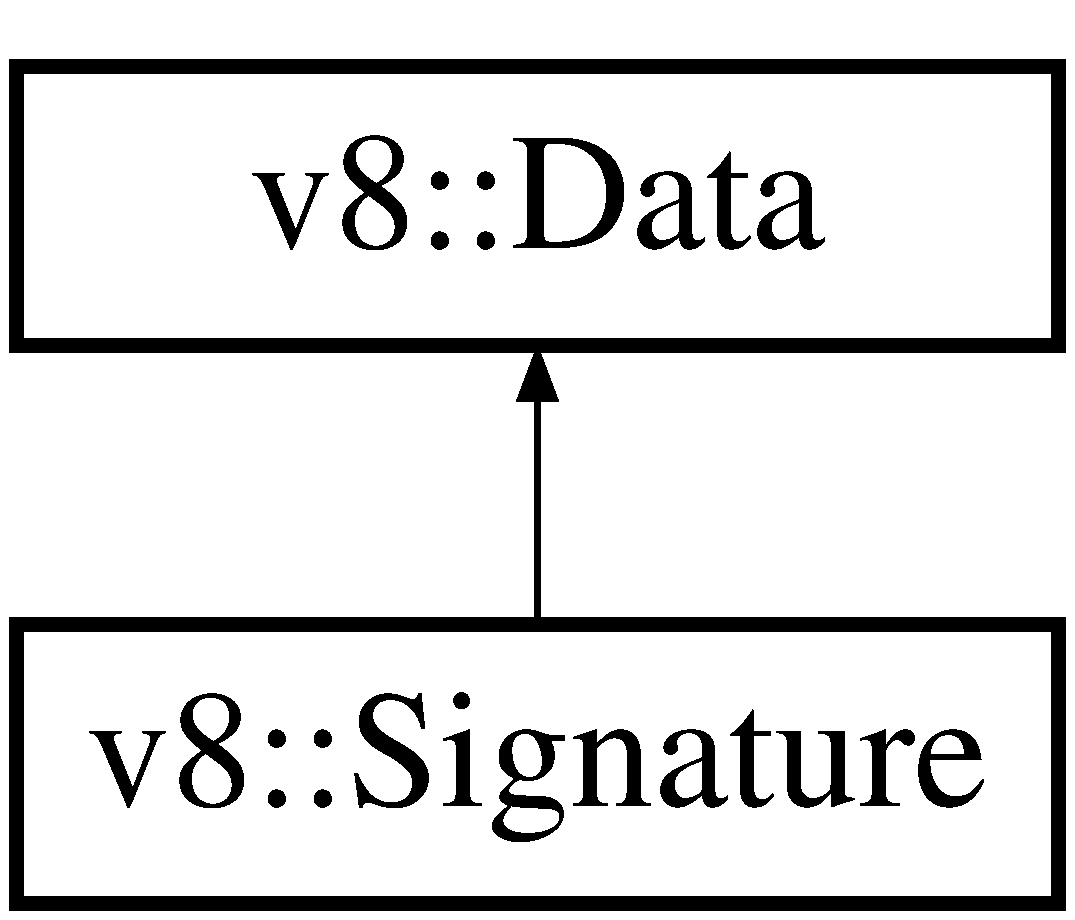
\includegraphics[height=2.000000cm]{classv8_1_1_signature}
\end{center}
\end{figure}
\subsection*{Static Public Member Functions}
\begin{DoxyCompactItemize}
\item 
\hypertarget{classv8_1_1_signature_a224e53e7ea0fc91b32758daf8b9a8718}{}static \hyperlink{classv8_1_1_local}{Local}$<$ \hyperlink{classv8_1_1_signature}{Signature} $>$ {\bfseries New} (\hyperlink{classv8_1_1_isolate}{Isolate} $\ast$isolate, \hyperlink{classv8_1_1_handle}{Handle}$<$ \hyperlink{classv8_1_1_function_template}{Function\+Template} $>$ receiver=\hyperlink{classv8_1_1_handle}{Handle}$<$ \hyperlink{classv8_1_1_function_template}{Function\+Template} $>$(), int argc=0, \hyperlink{classv8_1_1_handle}{Handle}$<$ \hyperlink{classv8_1_1_function_template}{Function\+Template} $>$ argv\mbox{[}$\,$\mbox{]}=0)\label{classv8_1_1_signature_a224e53e7ea0fc91b32758daf8b9a8718}

\end{DoxyCompactItemize}


\subsection{Detailed Description}
A \hyperlink{classv8_1_1_signature}{Signature} specifies which receivers and arguments are valid parameters to a function. 

The documentation for this class was generated from the following file\+:\begin{DoxyCompactItemize}
\item 
deps/v8/include/v8.\+h\end{DoxyCompactItemize}

\hypertarget{structv8_1_1internal_1_1_smi_constants}{}\section{v8\+:\+:internal\+:\+:Smi\+Constants$<$ ptr\+\_\+size $>$ Struct Template Reference}
\label{structv8_1_1internal_1_1_smi_constants}\index{v8\+::internal\+::\+Smi\+Constants$<$ ptr\+\_\+size $>$@{v8\+::internal\+::\+Smi\+Constants$<$ ptr\+\_\+size $>$}}


The documentation for this struct was generated from the following file\+:\begin{DoxyCompactItemize}
\item 
deps/v8/include/v8.\+h\end{DoxyCompactItemize}

\hypertarget{structv8_1_1internal_1_1_smi_constants_3_014_01_4}{}\section{v8\+:\+:internal\+:\+:Smi\+Constants$<$ 4 $>$ Struct Template Reference}
\label{structv8_1_1internal_1_1_smi_constants_3_014_01_4}\index{v8\+::internal\+::\+Smi\+Constants$<$ 4 $>$@{v8\+::internal\+::\+Smi\+Constants$<$ 4 $>$}}
\subsection*{Static Public Member Functions}
\begin{DoxyCompactItemize}
\item 
\hypertarget{structv8_1_1internal_1_1_smi_constants_3_014_01_4_a535d6ae95fc91da9258e31d810048043}{}static int {\bfseries Smi\+To\+Int} (internal\+::\+Object $\ast$value)\label{structv8_1_1internal_1_1_smi_constants_3_014_01_4_a535d6ae95fc91da9258e31d810048043}

\end{DoxyCompactItemize}
\subsection*{Static Public Attributes}
\begin{DoxyCompactItemize}
\item 
\hypertarget{structv8_1_1internal_1_1_smi_constants_3_014_01_4_a37addf80dd66de1967373c7b3ded1b26}{}static const int {\bfseries k\+Smi\+Shift\+Size} = 0\label{structv8_1_1internal_1_1_smi_constants_3_014_01_4_a37addf80dd66de1967373c7b3ded1b26}

\item 
\hypertarget{structv8_1_1internal_1_1_smi_constants_3_014_01_4_a4a8b755d509d53e452f12c29f39b6bd8}{}static const int {\bfseries k\+Smi\+Value\+Size} = 31\label{structv8_1_1internal_1_1_smi_constants_3_014_01_4_a4a8b755d509d53e452f12c29f39b6bd8}

\end{DoxyCompactItemize}


The documentation for this struct was generated from the following file\+:\begin{DoxyCompactItemize}
\item 
deps/v8/include/v8.\+h\end{DoxyCompactItemize}

\hypertarget{structv8_1_1internal_1_1_smi_constants_3_018_01_4}{}\section{v8\+:\+:internal\+:\+:Smi\+Constants$<$ 8 $>$ Struct Template Reference}
\label{structv8_1_1internal_1_1_smi_constants_3_018_01_4}\index{v8\+::internal\+::\+Smi\+Constants$<$ 8 $>$@{v8\+::internal\+::\+Smi\+Constants$<$ 8 $>$}}
\subsection*{Static Public Member Functions}
\begin{DoxyCompactItemize}
\item 
\hypertarget{structv8_1_1internal_1_1_smi_constants_3_018_01_4_a39b02998985462ae1c8169e5c8ce7645}{}static int {\bfseries Smi\+To\+Int} (internal\+::\+Object $\ast$value)\label{structv8_1_1internal_1_1_smi_constants_3_018_01_4_a39b02998985462ae1c8169e5c8ce7645}

\end{DoxyCompactItemize}
\subsection*{Static Public Attributes}
\begin{DoxyCompactItemize}
\item 
\hypertarget{structv8_1_1internal_1_1_smi_constants_3_018_01_4_aac9343671e3b80204a817d9b2d77d6d4}{}static const int {\bfseries k\+Smi\+Shift\+Size} = 31\label{structv8_1_1internal_1_1_smi_constants_3_018_01_4_aac9343671e3b80204a817d9b2d77d6d4}

\item 
\hypertarget{structv8_1_1internal_1_1_smi_constants_3_018_01_4_ab039612e1c2ef7ea953f0fc0758cd16b}{}static const int {\bfseries k\+Smi\+Value\+Size} = 32\label{structv8_1_1internal_1_1_smi_constants_3_018_01_4_ab039612e1c2ef7ea953f0fc0758cd16b}

\end{DoxyCompactItemize}


The documentation for this struct was generated from the following file\+:\begin{DoxyCompactItemize}
\item 
deps/v8/include/v8.\+h\end{DoxyCompactItemize}

\hypertarget{classv8_1_1_stack_frame}{}\section{v8\+:\+:Stack\+Frame Class Reference}
\label{classv8_1_1_stack_frame}\index{v8\+::\+Stack\+Frame@{v8\+::\+Stack\+Frame}}


{\ttfamily \#include $<$v8.\+h$>$}

\subsection*{Public Member Functions}
\begin{DoxyCompactItemize}
\item 
int \hyperlink{classv8_1_1_stack_frame_a57886e590ac1a4c57ee6f6bf1009b5b1}{Get\+Line\+Number} () const 
\item 
int \hyperlink{classv8_1_1_stack_frame_a44eccfb1bf17221ab6f69e977f3aa3a2}{Get\+Column} () const 
\item 
int \hyperlink{classv8_1_1_stack_frame_ac449d55656f8b7638de3cf5f5530cb7a}{Get\+Script\+Id} () const 
\item 
\hyperlink{classv8_1_1_local}{Local}$<$ \hyperlink{classv8_1_1_string}{String} $>$ \hyperlink{classv8_1_1_stack_frame_ac9701a5687dd04bcf24fd02f62bbe1a8}{Get\+Script\+Name} () const 
\item 
\hyperlink{classv8_1_1_local}{Local}$<$ \hyperlink{classv8_1_1_string}{String} $>$ \hyperlink{classv8_1_1_stack_frame_ac9f436f4cb245d871fe7efce03edc0cc}{Get\+Script\+Name\+Or\+Source\+U\+R\+L} () const 
\item 
\hyperlink{classv8_1_1_local}{Local}$<$ \hyperlink{classv8_1_1_string}{String} $>$ \hyperlink{classv8_1_1_stack_frame_ac13cdea4b4253d82485e673de6264073}{Get\+Function\+Name} () const 
\item 
bool \hyperlink{classv8_1_1_stack_frame_ae45f4d6ff9398a00a0b6534c160ec0c7}{Is\+Eval} () const 
\item 
bool \hyperlink{classv8_1_1_stack_frame_ade01313f4a3f6b88691d9d544737f65c}{Is\+Constructor} () const 
\end{DoxyCompactItemize}


\subsection{Detailed Description}
A single Java\+Script stack frame. 

\subsection{Member Function Documentation}
\hypertarget{classv8_1_1_stack_frame_a44eccfb1bf17221ab6f69e977f3aa3a2}{}\index{v8\+::\+Stack\+Frame@{v8\+::\+Stack\+Frame}!Get\+Column@{Get\+Column}}
\index{Get\+Column@{Get\+Column}!v8\+::\+Stack\+Frame@{v8\+::\+Stack\+Frame}}
\subsubsection[{Get\+Column}]{\setlength{\rightskip}{0pt plus 5cm}int v8\+::\+Stack\+Frame\+::\+Get\+Column (
\begin{DoxyParamCaption}
{}
\end{DoxyParamCaption}
) const}\label{classv8_1_1_stack_frame_a44eccfb1bf17221ab6f69e977f3aa3a2}
Returns the 1-\/based column offset on the line for the associated function call. This method will return Message\+::k\+No\+Column\+Info if it is unable to retrieve the column number, or if k\+Column\+Offset was not passed as an option when capturing the \hyperlink{classv8_1_1_stack_trace}{Stack\+Trace}. \hypertarget{classv8_1_1_stack_frame_ac13cdea4b4253d82485e673de6264073}{}\index{v8\+::\+Stack\+Frame@{v8\+::\+Stack\+Frame}!Get\+Function\+Name@{Get\+Function\+Name}}
\index{Get\+Function\+Name@{Get\+Function\+Name}!v8\+::\+Stack\+Frame@{v8\+::\+Stack\+Frame}}
\subsubsection[{Get\+Function\+Name}]{\setlength{\rightskip}{0pt plus 5cm}{\bf Local}$<${\bf String}$>$ v8\+::\+Stack\+Frame\+::\+Get\+Function\+Name (
\begin{DoxyParamCaption}
{}
\end{DoxyParamCaption}
) const}\label{classv8_1_1_stack_frame_ac13cdea4b4253d82485e673de6264073}
Returns the name of the function associated with this stack frame. \hypertarget{classv8_1_1_stack_frame_a57886e590ac1a4c57ee6f6bf1009b5b1}{}\index{v8\+::\+Stack\+Frame@{v8\+::\+Stack\+Frame}!Get\+Line\+Number@{Get\+Line\+Number}}
\index{Get\+Line\+Number@{Get\+Line\+Number}!v8\+::\+Stack\+Frame@{v8\+::\+Stack\+Frame}}
\subsubsection[{Get\+Line\+Number}]{\setlength{\rightskip}{0pt plus 5cm}int v8\+::\+Stack\+Frame\+::\+Get\+Line\+Number (
\begin{DoxyParamCaption}
{}
\end{DoxyParamCaption}
) const}\label{classv8_1_1_stack_frame_a57886e590ac1a4c57ee6f6bf1009b5b1}
Returns the number, 1-\/based, of the line for the associate function call. This method will return Message\+::k\+No\+Line\+Number\+Info if it is unable to retrieve the line number, or if k\+Line\+Number was not passed as an option when capturing the \hyperlink{classv8_1_1_stack_trace}{Stack\+Trace}. \hypertarget{classv8_1_1_stack_frame_ac449d55656f8b7638de3cf5f5530cb7a}{}\index{v8\+::\+Stack\+Frame@{v8\+::\+Stack\+Frame}!Get\+Script\+Id@{Get\+Script\+Id}}
\index{Get\+Script\+Id@{Get\+Script\+Id}!v8\+::\+Stack\+Frame@{v8\+::\+Stack\+Frame}}
\subsubsection[{Get\+Script\+Id}]{\setlength{\rightskip}{0pt plus 5cm}int v8\+::\+Stack\+Frame\+::\+Get\+Script\+Id (
\begin{DoxyParamCaption}
{}
\end{DoxyParamCaption}
) const}\label{classv8_1_1_stack_frame_ac449d55656f8b7638de3cf5f5530cb7a}
Returns the id of the script for the function for this \hyperlink{classv8_1_1_stack_frame}{Stack\+Frame}. This method will return Message\+::k\+No\+Script\+Id\+Info if it is unable to retrieve the script id, or if k\+Script\+Id was not passed as an option when capturing the \hyperlink{classv8_1_1_stack_trace}{Stack\+Trace}. \hypertarget{classv8_1_1_stack_frame_ac9701a5687dd04bcf24fd02f62bbe1a8}{}\index{v8\+::\+Stack\+Frame@{v8\+::\+Stack\+Frame}!Get\+Script\+Name@{Get\+Script\+Name}}
\index{Get\+Script\+Name@{Get\+Script\+Name}!v8\+::\+Stack\+Frame@{v8\+::\+Stack\+Frame}}
\subsubsection[{Get\+Script\+Name}]{\setlength{\rightskip}{0pt plus 5cm}{\bf Local}$<${\bf String}$>$ v8\+::\+Stack\+Frame\+::\+Get\+Script\+Name (
\begin{DoxyParamCaption}
{}
\end{DoxyParamCaption}
) const}\label{classv8_1_1_stack_frame_ac9701a5687dd04bcf24fd02f62bbe1a8}
Returns the name of the resource that contains the script for the function for this \hyperlink{classv8_1_1_stack_frame}{Stack\+Frame}. \hypertarget{classv8_1_1_stack_frame_ac9f436f4cb245d871fe7efce03edc0cc}{}\index{v8\+::\+Stack\+Frame@{v8\+::\+Stack\+Frame}!Get\+Script\+Name\+Or\+Source\+U\+R\+L@{Get\+Script\+Name\+Or\+Source\+U\+R\+L}}
\index{Get\+Script\+Name\+Or\+Source\+U\+R\+L@{Get\+Script\+Name\+Or\+Source\+U\+R\+L}!v8\+::\+Stack\+Frame@{v8\+::\+Stack\+Frame}}
\subsubsection[{Get\+Script\+Name\+Or\+Source\+U\+R\+L}]{\setlength{\rightskip}{0pt plus 5cm}{\bf Local}$<${\bf String}$>$ v8\+::\+Stack\+Frame\+::\+Get\+Script\+Name\+Or\+Source\+U\+R\+L (
\begin{DoxyParamCaption}
{}
\end{DoxyParamCaption}
) const}\label{classv8_1_1_stack_frame_ac9f436f4cb245d871fe7efce03edc0cc}
Returns the name of the resource that contains the script for the function for this \hyperlink{classv8_1_1_stack_frame}{Stack\+Frame} or source\+U\+R\+L value if the script name is undefined and its source ends with //\# source\+U\+R\+L=... string or deprecated //@ source\+U\+R\+L=... string. \hypertarget{classv8_1_1_stack_frame_ade01313f4a3f6b88691d9d544737f65c}{}\index{v8\+::\+Stack\+Frame@{v8\+::\+Stack\+Frame}!Is\+Constructor@{Is\+Constructor}}
\index{Is\+Constructor@{Is\+Constructor}!v8\+::\+Stack\+Frame@{v8\+::\+Stack\+Frame}}
\subsubsection[{Is\+Constructor}]{\setlength{\rightskip}{0pt plus 5cm}bool v8\+::\+Stack\+Frame\+::\+Is\+Constructor (
\begin{DoxyParamCaption}
{}
\end{DoxyParamCaption}
) const}\label{classv8_1_1_stack_frame_ade01313f4a3f6b88691d9d544737f65c}
Returns whether or not the associated function is called as a constructor via \char`\"{}new\char`\"{}. \hypertarget{classv8_1_1_stack_frame_ae45f4d6ff9398a00a0b6534c160ec0c7}{}\index{v8\+::\+Stack\+Frame@{v8\+::\+Stack\+Frame}!Is\+Eval@{Is\+Eval}}
\index{Is\+Eval@{Is\+Eval}!v8\+::\+Stack\+Frame@{v8\+::\+Stack\+Frame}}
\subsubsection[{Is\+Eval}]{\setlength{\rightskip}{0pt plus 5cm}bool v8\+::\+Stack\+Frame\+::\+Is\+Eval (
\begin{DoxyParamCaption}
{}
\end{DoxyParamCaption}
) const}\label{classv8_1_1_stack_frame_ae45f4d6ff9398a00a0b6534c160ec0c7}
Returns whether or not the associated function is compiled via a call to eval(). 

The documentation for this class was generated from the following file\+:\begin{DoxyCompactItemize}
\item 
deps/v8/include/v8.\+h\end{DoxyCompactItemize}

\hypertarget{classv8_1_1_stack_trace}{}\section{v8\+:\+:Stack\+Trace Class Reference}
\label{classv8_1_1_stack_trace}\index{v8\+::\+Stack\+Trace@{v8\+::\+Stack\+Trace}}


{\ttfamily \#include $<$v8.\+h$>$}

\subsection*{Public Types}
\begin{DoxyCompactItemize}
\item 
enum \hyperlink{classv8_1_1_stack_trace_a9704e4a37949eb8eb8ccddbddf161492}{Stack\+Trace\+Options} \{ \\*
{\bfseries k\+Line\+Number} = 1, 
{\bfseries k\+Column\+Offset} = 1 $<$$<$ 1 $\vert$ k\+Line\+Number, 
{\bfseries k\+Script\+Name} = 1 $<$$<$ 2, 
{\bfseries k\+Function\+Name} = 1 $<$$<$ 3, 
\\*
{\bfseries k\+Is\+Eval} = 1 $<$$<$ 4, 
{\bfseries k\+Is\+Constructor} = 1 $<$$<$ 5, 
{\bfseries k\+Script\+Name\+Or\+Source\+U\+R\+L} = 1 $<$$<$ 6, 
{\bfseries k\+Overview} = k\+Line\+Number $\vert$ k\+Column\+Offset $\vert$ k\+Script\+Name $\vert$ k\+Function\+Name, 
\\*
{\bfseries k\+Detailed} = k\+Overview $\vert$ k\+Is\+Eval $\vert$ k\+Is\+Constructor $\vert$ k\+Script\+Name\+Or\+Source\+U\+R\+L
 \}
\end{DoxyCompactItemize}
\subsection*{Public Member Functions}
\begin{DoxyCompactItemize}
\item 
\hyperlink{classv8_1_1_local}{Local}$<$ \hyperlink{classv8_1_1_stack_frame}{Stack\+Frame} $>$ \hyperlink{classv8_1_1_stack_trace_a6fd5ba809b5d87032d70d32f0b1a80e8}{Get\+Frame} (uint32\+\_\+t index) const 
\item 
int \hyperlink{classv8_1_1_stack_trace_aafafebce6c034f1f6f4a870e8f52431e}{Get\+Frame\+Count} () const 
\item 
\hyperlink{classv8_1_1_local}{Local}$<$ \hyperlink{classv8_1_1_array}{Array} $>$ \hyperlink{classv8_1_1_stack_trace_abd36f712b3ab986b572aa259b06bf5bd}{As\+Array} ()
\end{DoxyCompactItemize}
\subsection*{Static Public Member Functions}
\begin{DoxyCompactItemize}
\item 
static \hyperlink{classv8_1_1_local}{Local}$<$ \hyperlink{classv8_1_1_stack_trace}{Stack\+Trace} $>$ \hyperlink{classv8_1_1_stack_trace_a1fe0944a73e18aaab8437bbc72a194c7}{Current\+Stack\+Trace} (int frame\+\_\+limit, \hyperlink{classv8_1_1_stack_trace_a9704e4a37949eb8eb8ccddbddf161492}{Stack\+Trace\+Options} options=k\+Overview)
\end{DoxyCompactItemize}


\subsection{Detailed Description}
Representation of a Java\+Script stack trace. The information collected is a snapshot of the execution stack and the information remains valid after execution continues. 

\subsection{Member Enumeration Documentation}
\hypertarget{classv8_1_1_stack_trace_a9704e4a37949eb8eb8ccddbddf161492}{}\index{v8\+::\+Stack\+Trace@{v8\+::\+Stack\+Trace}!Stack\+Trace\+Options@{Stack\+Trace\+Options}}
\index{Stack\+Trace\+Options@{Stack\+Trace\+Options}!v8\+::\+Stack\+Trace@{v8\+::\+Stack\+Trace}}
\subsubsection[{Stack\+Trace\+Options}]{\setlength{\rightskip}{0pt plus 5cm}enum {\bf v8\+::\+Stack\+Trace\+::\+Stack\+Trace\+Options}}\label{classv8_1_1_stack_trace_a9704e4a37949eb8eb8ccddbddf161492}
Flags that determine what information is placed captured for each \hyperlink{classv8_1_1_stack_frame}{Stack\+Frame} when grabbing the current stack trace. 

\subsection{Member Function Documentation}
\hypertarget{classv8_1_1_stack_trace_abd36f712b3ab986b572aa259b06bf5bd}{}\index{v8\+::\+Stack\+Trace@{v8\+::\+Stack\+Trace}!As\+Array@{As\+Array}}
\index{As\+Array@{As\+Array}!v8\+::\+Stack\+Trace@{v8\+::\+Stack\+Trace}}
\subsubsection[{As\+Array}]{\setlength{\rightskip}{0pt plus 5cm}{\bf Local}$<${\bf Array}$>$ v8\+::\+Stack\+Trace\+::\+As\+Array (
\begin{DoxyParamCaption}
{}
\end{DoxyParamCaption}
)}\label{classv8_1_1_stack_trace_abd36f712b3ab986b572aa259b06bf5bd}
Returns \hyperlink{classv8_1_1_stack_trace}{Stack\+Trace} as a \hyperlink{classv8_1_1_array}{v8\+::\+Array} that contains \hyperlink{classv8_1_1_stack_frame}{Stack\+Frame} objects. \hypertarget{classv8_1_1_stack_trace_a1fe0944a73e18aaab8437bbc72a194c7}{}\index{v8\+::\+Stack\+Trace@{v8\+::\+Stack\+Trace}!Current\+Stack\+Trace@{Current\+Stack\+Trace}}
\index{Current\+Stack\+Trace@{Current\+Stack\+Trace}!v8\+::\+Stack\+Trace@{v8\+::\+Stack\+Trace}}
\subsubsection[{Current\+Stack\+Trace}]{\setlength{\rightskip}{0pt plus 5cm}static {\bf Local}$<${\bf Stack\+Trace}$>$ v8\+::\+Stack\+Trace\+::\+Current\+Stack\+Trace (
\begin{DoxyParamCaption}
\item[{int}]{frame\+\_\+limit, }
\item[{{\bf Stack\+Trace\+Options}}]{options = {\ttfamily kOverview}}
\end{DoxyParamCaption}
)\hspace{0.3cm}{\ttfamily [static]}}\label{classv8_1_1_stack_trace_a1fe0944a73e18aaab8437bbc72a194c7}
Grab a snapshot of the the current Java\+Script execution stack.


\begin{DoxyParams}{Parameters}
{\em frame\+\_\+limit} & The maximum number of stack frames we want to capture. \\
\hline
{\em options} & Enumerates the set of things we will capture for each \hyperlink{classv8_1_1_stack_frame}{Stack\+Frame}. \\
\hline
\end{DoxyParams}
\hypertarget{classv8_1_1_stack_trace_a6fd5ba809b5d87032d70d32f0b1a80e8}{}\index{v8\+::\+Stack\+Trace@{v8\+::\+Stack\+Trace}!Get\+Frame@{Get\+Frame}}
\index{Get\+Frame@{Get\+Frame}!v8\+::\+Stack\+Trace@{v8\+::\+Stack\+Trace}}
\subsubsection[{Get\+Frame}]{\setlength{\rightskip}{0pt plus 5cm}{\bf Local}$<${\bf Stack\+Frame}$>$ v8\+::\+Stack\+Trace\+::\+Get\+Frame (
\begin{DoxyParamCaption}
\item[{uint32\+\_\+t}]{index}
\end{DoxyParamCaption}
) const}\label{classv8_1_1_stack_trace_a6fd5ba809b5d87032d70d32f0b1a80e8}
Returns a \hyperlink{classv8_1_1_stack_frame}{Stack\+Frame} at a particular index. \hypertarget{classv8_1_1_stack_trace_aafafebce6c034f1f6f4a870e8f52431e}{}\index{v8\+::\+Stack\+Trace@{v8\+::\+Stack\+Trace}!Get\+Frame\+Count@{Get\+Frame\+Count}}
\index{Get\+Frame\+Count@{Get\+Frame\+Count}!v8\+::\+Stack\+Trace@{v8\+::\+Stack\+Trace}}
\subsubsection[{Get\+Frame\+Count}]{\setlength{\rightskip}{0pt plus 5cm}int v8\+::\+Stack\+Trace\+::\+Get\+Frame\+Count (
\begin{DoxyParamCaption}
{}
\end{DoxyParamCaption}
) const}\label{classv8_1_1_stack_trace_aafafebce6c034f1f6f4a870e8f52431e}
Returns the number of Stack\+Frames. 

The documentation for this class was generated from the following file\+:\begin{DoxyCompactItemize}
\item 
deps/v8/include/v8.\+h\end{DoxyCompactItemize}

\hypertarget{classv8_1_1_string}{}\section{v8\+:\+:String Class Reference}
\label{classv8_1_1_string}\index{v8\+::\+String@{v8\+::\+String}}


{\ttfamily \#include $<$v8.\+h$>$}

Inheritance diagram for v8\+:\+:String\+:\begin{figure}[H]
\begin{center}
\leavevmode
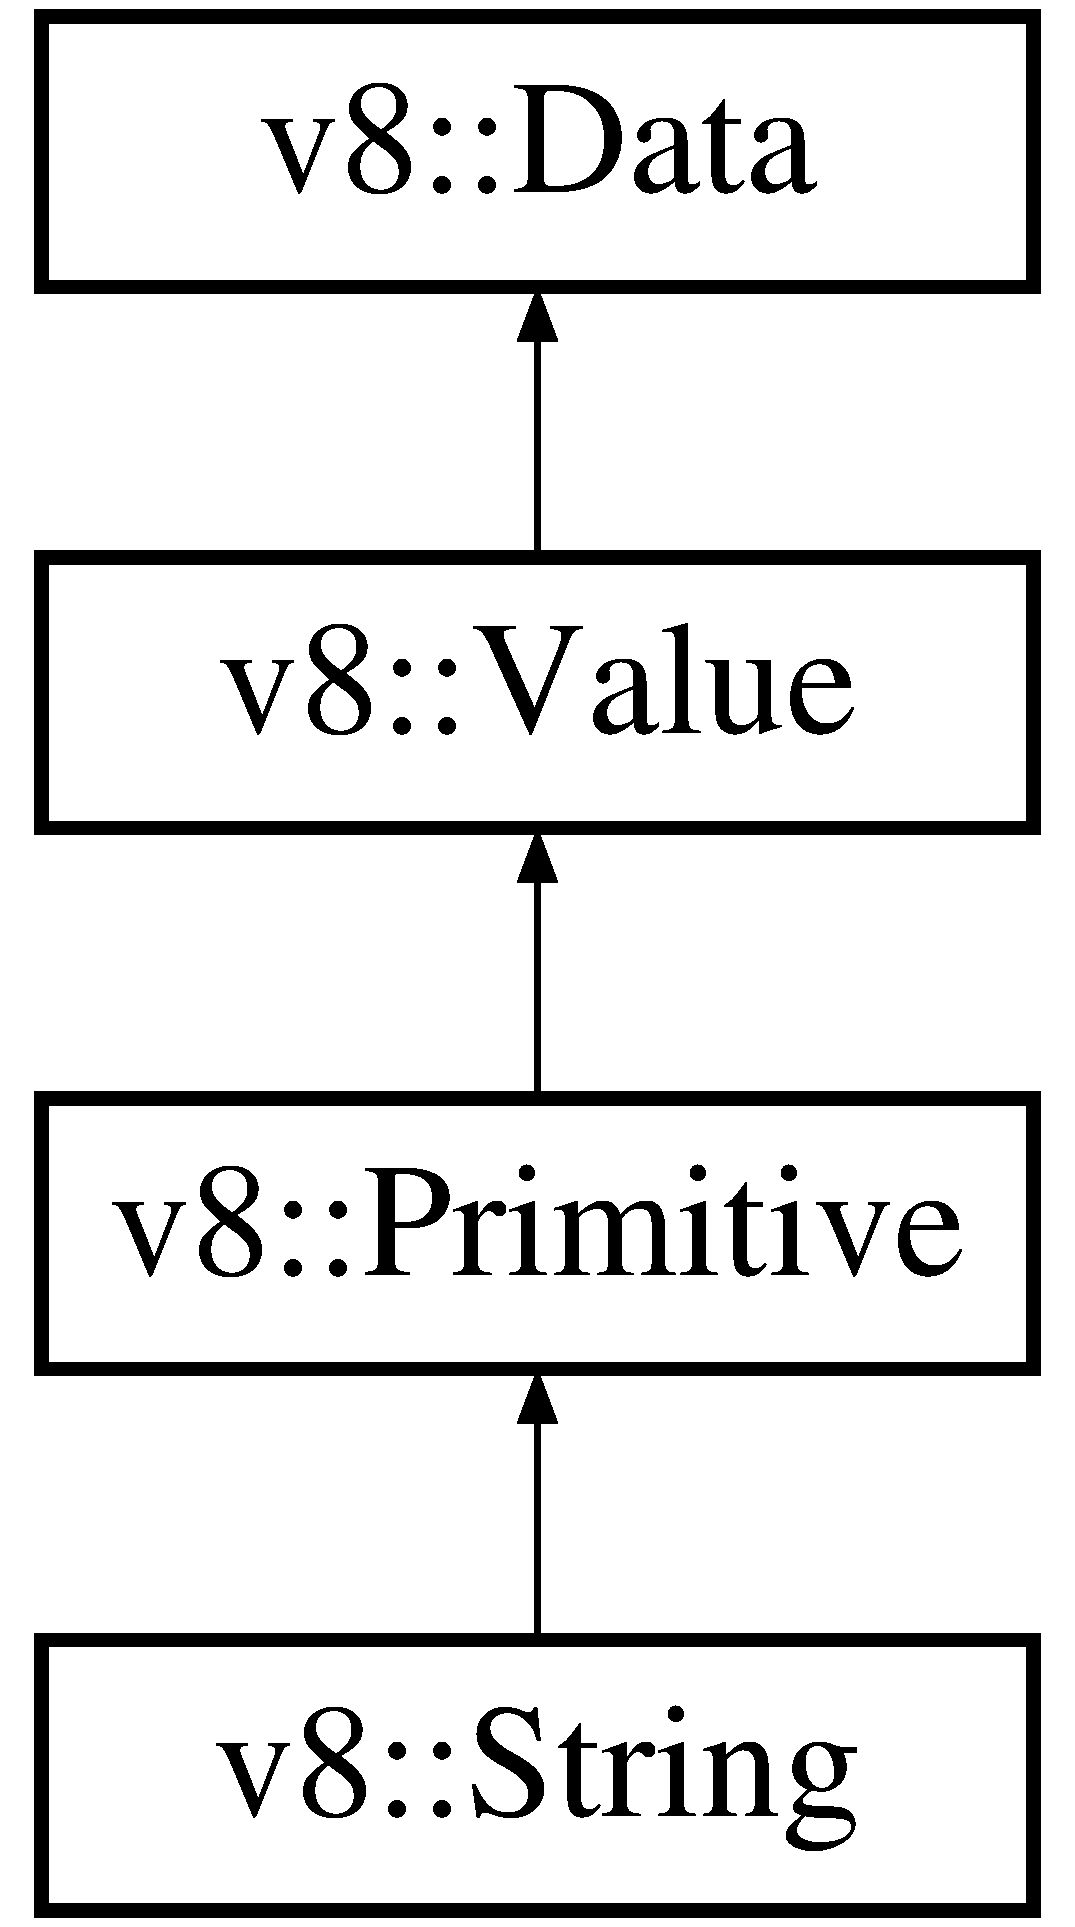
\includegraphics[height=5.000000cm]{classv8_1_1_string}
\end{center}
\end{figure}
\subsection*{Classes}
\begin{DoxyCompactItemize}
\item 
class \hyperlink{classv8_1_1_string_1_1_external_one_byte_string_resource}{External\+One\+Byte\+String\+Resource}
\item 
class \hyperlink{classv8_1_1_string_1_1_external_string_resource}{External\+String\+Resource}
\item 
class \hyperlink{classv8_1_1_string_1_1_external_string_resource_base}{External\+String\+Resource\+Base}
\item 
class \hyperlink{classv8_1_1_string_1_1_utf8_value}{Utf8\+Value}
\item 
class \hyperlink{classv8_1_1_string_1_1_value}{Value}
\end{DoxyCompactItemize}
\subsection*{Public Types}
\begin{DoxyCompactItemize}
\item 
\hypertarget{classv8_1_1_string_a2f4a2e9516c246eef602b889ce049c49}{}enum {\bfseries Encoding} \{ {\bfseries U\+N\+K\+N\+O\+W\+N\+\_\+\+E\+N\+C\+O\+D\+I\+N\+G} = 0x1, 
{\bfseries T\+W\+O\+\_\+\+B\+Y\+T\+E\+\_\+\+E\+N\+C\+O\+D\+I\+N\+G} = 0x0, 
{\bfseries O\+N\+E\+\_\+\+B\+Y\+T\+E\+\_\+\+E\+N\+C\+O\+D\+I\+N\+G} = 0x4
 \}\label{classv8_1_1_string_a2f4a2e9516c246eef602b889ce049c49}

\item 
enum \hyperlink{classv8_1_1_string_a9ce7f1458ffd08f8eb2b9c8dc056e616}{Write\+Options} \{ \\*
{\bfseries N\+O\+\_\+\+O\+P\+T\+I\+O\+N\+S} = 0, 
{\bfseries H\+I\+N\+T\+\_\+\+M\+A\+N\+Y\+\_\+\+W\+R\+I\+T\+E\+S\+\_\+\+E\+X\+P\+E\+C\+T\+E\+D} = 1, 
{\bfseries N\+O\+\_\+\+N\+U\+L\+L\+\_\+\+T\+E\+R\+M\+I\+N\+A\+T\+I\+O\+N} = 2, 
{\bfseries P\+R\+E\+S\+E\+R\+V\+E\+\_\+\+O\+N\+E\+\_\+\+B\+Y\+T\+E\+\_\+\+N\+U\+L\+L} = 4, 
\\*
{\bfseries R\+E\+P\+L\+A\+C\+E\+\_\+\+I\+N\+V\+A\+L\+I\+D\+\_\+\+U\+T\+F8} = 8
 \}
\item 
\hypertarget{classv8_1_1_string_a37620fb9fdc9b72ec9eea2a2aafaddee}{}enum {\bfseries New\+String\+Type} \{ {\bfseries k\+Normal\+String} = static\+\_\+cast$<$int$>$(v8\+:\+:New\+String\+Type\+:\+:k\+Normal), 
{\bfseries k\+Internalized\+String} = static\+\_\+cast$<$int$>$(v8\+:\+:New\+String\+Type\+:\+:k\+Internalized)
 \}\label{classv8_1_1_string_a37620fb9fdc9b72ec9eea2a2aafaddee}

\end{DoxyCompactItemize}
\subsection*{Public Member Functions}
\begin{DoxyCompactItemize}
\item 
int \hyperlink{classv8_1_1_string_a94353cd764d2bf0cda141714c3c9eb6c}{Length} () const 
\item 
int \hyperlink{classv8_1_1_string_afb2bb302d3ffe807e66a0797d6ac4189}{Utf8\+Length} () const 
\item 
bool \hyperlink{classv8_1_1_string_a2e6771bd8fbd0e2d1fa01811d3e8c7dc}{Is\+One\+Byte} () const 
\item 
bool \hyperlink{classv8_1_1_string_a4ae1fe1175bd5b96bfa53f5f5ee835e9}{Contains\+Only\+One\+Byte} () const 
\item 
\hypertarget{classv8_1_1_string_ab1ee96f8adf969958faeff9eced9a56f}{}int {\bfseries Write} (uint16\+\_\+t $\ast$buffer, int start=0, int length=-\/1, int options=N\+O\+\_\+\+O\+P\+T\+I\+O\+N\+S) const \label{classv8_1_1_string_ab1ee96f8adf969958faeff9eced9a56f}

\item 
\hypertarget{classv8_1_1_string_a61114324ef659345f04b2730679eb456}{}int {\bfseries Write\+One\+Byte} (uint8\+\_\+t $\ast$buffer, int start=0, int length=-\/1, int options=N\+O\+\_\+\+O\+P\+T\+I\+O\+N\+S) const \label{classv8_1_1_string_a61114324ef659345f04b2730679eb456}

\item 
\hypertarget{classv8_1_1_string_ad62145c723fa0ce55095223223263f41}{}int {\bfseries Write\+Utf8} (char $\ast$buffer, int length=-\/1, int $\ast$nchars\+\_\+ref=N\+U\+L\+L, int options=N\+O\+\_\+\+O\+P\+T\+I\+O\+N\+S) const \label{classv8_1_1_string_ad62145c723fa0ce55095223223263f41}

\item 
bool \hyperlink{classv8_1_1_string_abbf623aabba9446cd57af14018877398}{Is\+External} () const 
\item 
bool \hyperlink{classv8_1_1_string_a0911614baa308fc270126390e39e4dd1}{Is\+External\+One\+Byte} () const 
\item 
V8\+\_\+\+I\+N\+L\+I\+N\+E \hyperlink{classv8_1_1_string_1_1_external_string_resource_base}{External\+String\+Resource\+Base} $\ast$ \hyperlink{classv8_1_1_string_a471cf0e3ca135d839e59d25da66894e0}{Get\+External\+String\+Resource\+Base} (Encoding $\ast$encoding\+\_\+out) const 
\item 
V8\+\_\+\+I\+N\+L\+I\+N\+E \hyperlink{classv8_1_1_string_1_1_external_string_resource}{External\+String\+Resource} $\ast$ \hyperlink{classv8_1_1_string_a1a78c6fe39dbdd6322ca576e224f0cba}{Get\+External\+String\+Resource} () const 
\item 
const \hyperlink{classv8_1_1_string_1_1_external_one_byte_string_resource}{External\+One\+Byte\+String\+Resource} $\ast$ \hyperlink{classv8_1_1_string_ac8497aa76a576f965042812d5efa95b2}{Get\+External\+One\+Byte\+String\+Resource} () const 
\item 
bool \hyperlink{classv8_1_1_string_a5efd1eba40c1fa8a6aae2c4a175a63be}{Make\+External} (\hyperlink{classv8_1_1_string_1_1_external_string_resource}{External\+String\+Resource} $\ast$resource)
\item 
bool \hyperlink{classv8_1_1_string_a607d632c720eec5133649f522aefa944}{Make\+External} (\hyperlink{classv8_1_1_string_1_1_external_one_byte_string_resource}{External\+One\+Byte\+String\+Resource} $\ast$resource)
\item 
bool \hyperlink{classv8_1_1_string_a0fe076838af046506ffebbfadcde812a}{Can\+Make\+External} ()
\end{DoxyCompactItemize}
\subsection*{Static Public Member Functions}
\begin{DoxyCompactItemize}
\item 
static V8\+\_\+\+I\+N\+L\+I\+N\+E \hyperlink{classv8_1_1_local}{v8\+::\+Local}$<$ \hyperlink{classv8_1_1_string}{v8\+::\+String} $>$ \hyperlink{classv8_1_1_string_aa393d47baa54467fe57001065e49194b}{Empty} (\hyperlink{classv8_1_1_isolate}{Isolate} $\ast$isolate)
\item 
\hypertarget{classv8_1_1_string_a826d60798dc152cea64a7636737b03b9}{}static V8\+\_\+\+I\+N\+L\+I\+N\+E \hyperlink{classv8_1_1_string}{String} $\ast$ {\bfseries Cast} (\hyperlink{classv8_1_1_value}{v8\+::\+Value} $\ast$obj)\label{classv8_1_1_string_a826d60798dc152cea64a7636737b03b9}

\item 
static \hyperlink{classv8_1_1_string_aa9d64688e3535b3daabafcc46a59ce5a}{V8\+\_\+\+D\+E\+P\+R\+E\+C\+A\+T\+E\+\_\+\+S\+O\+O\+N} (\char`\"{}Use maybe version\char`\"{}, Local$<$ \hyperlink{classv8_1_1_string}{String} $>$ \hyperlink{classv8_1_1_string_a851bcf20fecb01b97f14131ce609f701}{New\+From\+Utf8}(\hyperlink{classv8_1_1_isolate}{Isolate} $\ast$isolate, const char $\ast$data, New\+String\+Type type=k\+Normal\+String, int length=-\/1))
\item 
static V8\+\_\+\+W\+A\+R\+N\+\_\+\+U\+N\+U\+S\+E\+D\+\_\+\+R\+E\+S\+U\+L\+T \hyperlink{classv8_1_1_maybe_local}{Maybe\+Local}$<$ \hyperlink{classv8_1_1_string}{String} $>$ \hyperlink{classv8_1_1_string_a851bcf20fecb01b97f14131ce609f701}{New\+From\+Utf8} (\hyperlink{classv8_1_1_isolate}{Isolate} $\ast$isolate, const char $\ast$data, v8\+::\+New\+String\+Type type, int length=-\/1)
\item 
static \hyperlink{classv8_1_1_string_a97b6caaf4674979cfbd2dfd6c12e48f3}{V8\+\_\+\+D\+E\+P\+R\+E\+C\+A\+T\+E\+\_\+\+S\+O\+O\+N} (\char`\"{}Use maybe version\char`\"{}, Local$<$ \hyperlink{classv8_1_1_string}{String} $>$ \hyperlink{classv8_1_1_string_a2b8cf518523a62d97360c07ed33d8aa6}{New\+From\+One\+Byte}(\hyperlink{classv8_1_1_isolate}{Isolate} $\ast$isolate, const uint8\+\_\+t $\ast$data, New\+String\+Type type=k\+Normal\+String, int length=-\/1))
\item 
static V8\+\_\+\+W\+A\+R\+N\+\_\+\+U\+N\+U\+S\+E\+D\+\_\+\+R\+E\+S\+U\+L\+T \hyperlink{classv8_1_1_maybe_local}{Maybe\+Local}$<$ \hyperlink{classv8_1_1_string}{String} $>$ \hyperlink{classv8_1_1_string_a2b8cf518523a62d97360c07ed33d8aa6}{New\+From\+One\+Byte} (\hyperlink{classv8_1_1_isolate}{Isolate} $\ast$isolate, const uint8\+\_\+t $\ast$data, v8\+::\+New\+String\+Type type, int length=-\/1)
\item 
static \hyperlink{classv8_1_1_string_aeab948105979e2ffd61eb552b0da4e50}{V8\+\_\+\+D\+E\+P\+R\+E\+C\+A\+T\+E\+\_\+\+S\+O\+O\+N} (\char`\"{}Use maybe version\char`\"{}, Local$<$ \hyperlink{classv8_1_1_string}{String} $>$ \hyperlink{classv8_1_1_string_aaad4c7c856c29d79db85994c301fe601}{New\+From\+Two\+Byte}(\hyperlink{classv8_1_1_isolate}{Isolate} $\ast$isolate, const uint16\+\_\+t $\ast$data, New\+String\+Type type=k\+Normal\+String, int length=-\/1))
\item 
static V8\+\_\+\+W\+A\+R\+N\+\_\+\+U\+N\+U\+S\+E\+D\+\_\+\+R\+E\+S\+U\+L\+T \hyperlink{classv8_1_1_maybe_local}{Maybe\+Local}$<$ \hyperlink{classv8_1_1_string}{String} $>$ \hyperlink{classv8_1_1_string_aaad4c7c856c29d79db85994c301fe601}{New\+From\+Two\+Byte} (\hyperlink{classv8_1_1_isolate}{Isolate} $\ast$isolate, const uint16\+\_\+t $\ast$data, v8\+::\+New\+String\+Type type, int length=-\/1)
\item 
static \hyperlink{classv8_1_1_local}{Local}$<$ \hyperlink{classv8_1_1_string}{String} $>$ \hyperlink{classv8_1_1_string_a3d0b9c9208cf5054adb048e360fb73ff}{Concat} (\hyperlink{classv8_1_1_local}{Handle}$<$ \hyperlink{classv8_1_1_string}{String} $>$ left, \hyperlink{classv8_1_1_local}{Handle}$<$ \hyperlink{classv8_1_1_string}{String} $>$ right)
\item 
static \hyperlink{classv8_1_1_string_affb615b7b4aad75d51d60ed1672a6762}{V8\+\_\+\+D\+E\+P\+R\+E\+C\+A\+T\+E\+\_\+\+S\+O\+O\+N} (\char`\"{}Use maybe version\char`\"{}, Local$<$ \hyperlink{classv8_1_1_string}{String} $>$ New\+External(\hyperlink{classv8_1_1_isolate}{Isolate} $\ast$isolate, \hyperlink{classv8_1_1_string_1_1_external_string_resource}{External\+String\+Resource} $\ast$resource))
\item 
\hypertarget{classv8_1_1_string_ad0491e4a3506df9ef9bfc08fca0d7a34}{}static V8\+\_\+\+W\+A\+R\+N\+\_\+\+U\+N\+U\+S\+E\+D\+\_\+\+R\+E\+S\+U\+L\+T \hyperlink{classv8_1_1_maybe_local}{Maybe\+Local}$<$ \hyperlink{classv8_1_1_string}{String} $>$ {\bfseries New\+External\+Two\+Byte} (\hyperlink{classv8_1_1_isolate}{Isolate} $\ast$isolate, \hyperlink{classv8_1_1_string_1_1_external_string_resource}{External\+String\+Resource} $\ast$resource)\label{classv8_1_1_string_ad0491e4a3506df9ef9bfc08fca0d7a34}

\item 
static \hyperlink{classv8_1_1_string_ad7186b5cfdddffbee8235a7216f31a67}{V8\+\_\+\+D\+E\+P\+R\+E\+C\+A\+T\+E\+\_\+\+S\+O\+O\+N} (\char`\"{}Use maybe version\char`\"{}, Local$<$ \hyperlink{classv8_1_1_string}{String} $>$ New\+External(\hyperlink{classv8_1_1_isolate}{Isolate} $\ast$isolate, \hyperlink{classv8_1_1_string_1_1_external_one_byte_string_resource}{External\+One\+Byte\+String\+Resource} $\ast$resource))
\item 
\hypertarget{classv8_1_1_string_a43edc2bcb1bf2a06f306ea9554042f24}{}static V8\+\_\+\+W\+A\+R\+N\+\_\+\+U\+N\+U\+S\+E\+D\+\_\+\+R\+E\+S\+U\+L\+T \hyperlink{classv8_1_1_maybe_local}{Maybe\+Local}$<$ \hyperlink{classv8_1_1_string}{String} $>$ {\bfseries New\+External\+One\+Byte} (\hyperlink{classv8_1_1_isolate}{Isolate} $\ast$isolate, \hyperlink{classv8_1_1_string_1_1_external_one_byte_string_resource}{External\+One\+Byte\+String\+Resource} $\ast$resource)\label{classv8_1_1_string_a43edc2bcb1bf2a06f306ea9554042f24}

\end{DoxyCompactItemize}
\subsection*{Static Public Attributes}
\begin{DoxyCompactItemize}
\item 
\hypertarget{classv8_1_1_string_a51272e8a71006385863586afb2bb4a62}{}static const int {\bfseries k\+Max\+Length} = (1 $<$$<$ 28) -\/ 16\label{classv8_1_1_string_a51272e8a71006385863586afb2bb4a62}

\end{DoxyCompactItemize}


\subsection{Detailed Description}
A Java\+Script string value (E\+C\+M\+A-\/262, 4.\+3.\+17). 

\subsection{Member Enumeration Documentation}
\hypertarget{classv8_1_1_string_a9ce7f1458ffd08f8eb2b9c8dc056e616}{}\index{v8\+::\+String@{v8\+::\+String}!Write\+Options@{Write\+Options}}
\index{Write\+Options@{Write\+Options}!v8\+::\+String@{v8\+::\+String}}
\subsubsection[{Write\+Options}]{\setlength{\rightskip}{0pt plus 5cm}enum {\bf v8\+::\+String\+::\+Write\+Options}}\label{classv8_1_1_string_a9ce7f1458ffd08f8eb2b9c8dc056e616}
Write the contents of the string to an external buffer. If no arguments are given, expects the buffer to be large enough to hold the entire string and N\+U\+L\+L terminator. Copies the contents of the string and the N\+U\+L\+L terminator into the buffer.

Write\+Utf8 will not write partial U\+T\+F-\/8 sequences, preferring to stop before the end of the buffer.

Copies up to length characters into the output buffer. Only null-\/terminates if there is enough space in the buffer.


\begin{DoxyParams}{Parameters}
{\em buffer} & The buffer into which the string will be copied. \\
\hline
{\em start} & The starting position within the string at which copying begins. \\
\hline
{\em length} & The number of characters to copy from the string. For Write\+Utf8 the number of bytes in the buffer. \\
\hline
{\em nchars\+\_\+ref} & The number of characters written, can be N\+U\+L\+L. \\
\hline
{\em options} & Various options that might affect performance of this or subsequent operations. \\
\hline
\end{DoxyParams}
\begin{DoxyReturn}{Returns}
The number of characters copied to the buffer excluding the null terminator. For Write\+Utf8\+: The number of bytes copied to the buffer including the null terminator (if written). 
\end{DoxyReturn}


\subsection{Member Function Documentation}
\hypertarget{classv8_1_1_string_a0fe076838af046506ffebbfadcde812a}{}\index{v8\+::\+String@{v8\+::\+String}!Can\+Make\+External@{Can\+Make\+External}}
\index{Can\+Make\+External@{Can\+Make\+External}!v8\+::\+String@{v8\+::\+String}}
\subsubsection[{Can\+Make\+External}]{\setlength{\rightskip}{0pt plus 5cm}bool v8\+::\+String\+::\+Can\+Make\+External (
\begin{DoxyParamCaption}
{}
\end{DoxyParamCaption}
)}\label{classv8_1_1_string_a0fe076838af046506ffebbfadcde812a}
Returns true if this string can be made external. \hypertarget{classv8_1_1_string_a3d0b9c9208cf5054adb048e360fb73ff}{}\index{v8\+::\+String@{v8\+::\+String}!Concat@{Concat}}
\index{Concat@{Concat}!v8\+::\+String@{v8\+::\+String}}
\subsubsection[{Concat}]{\setlength{\rightskip}{0pt plus 5cm}static {\bf Local}$<${\bf String}$>$ v8\+::\+String\+::\+Concat (
\begin{DoxyParamCaption}
\item[{{\bf Handle}$<$ {\bf String} $>$}]{left, }
\item[{{\bf Handle}$<$ {\bf String} $>$}]{right}
\end{DoxyParamCaption}
)\hspace{0.3cm}{\ttfamily [static]}}\label{classv8_1_1_string_a3d0b9c9208cf5054adb048e360fb73ff}
Creates a new string by concatenating the left and the right strings passed in as parameters. \hypertarget{classv8_1_1_string_a4ae1fe1175bd5b96bfa53f5f5ee835e9}{}\index{v8\+::\+String@{v8\+::\+String}!Contains\+Only\+One\+Byte@{Contains\+Only\+One\+Byte}}
\index{Contains\+Only\+One\+Byte@{Contains\+Only\+One\+Byte}!v8\+::\+String@{v8\+::\+String}}
\subsubsection[{Contains\+Only\+One\+Byte}]{\setlength{\rightskip}{0pt plus 5cm}bool v8\+::\+String\+::\+Contains\+Only\+One\+Byte (
\begin{DoxyParamCaption}
{}
\end{DoxyParamCaption}
) const}\label{classv8_1_1_string_a4ae1fe1175bd5b96bfa53f5f5ee835e9}
Returns whether this string contain only one byte data. Will read the entire string in some cases. \hypertarget{classv8_1_1_string_aa393d47baa54467fe57001065e49194b}{}\index{v8\+::\+String@{v8\+::\+String}!Empty@{Empty}}
\index{Empty@{Empty}!v8\+::\+String@{v8\+::\+String}}
\subsubsection[{Empty}]{\setlength{\rightskip}{0pt plus 5cm}{\bf Local}$<$ {\bf String} $>$ v8\+::\+String\+::\+Empty (
\begin{DoxyParamCaption}
\item[{{\bf Isolate} $\ast$}]{isolate}
\end{DoxyParamCaption}
)\hspace{0.3cm}{\ttfamily [static]}}\label{classv8_1_1_string_aa393d47baa54467fe57001065e49194b}
A zero length string. \hypertarget{classv8_1_1_string_ac8497aa76a576f965042812d5efa95b2}{}\index{v8\+::\+String@{v8\+::\+String}!Get\+External\+One\+Byte\+String\+Resource@{Get\+External\+One\+Byte\+String\+Resource}}
\index{Get\+External\+One\+Byte\+String\+Resource@{Get\+External\+One\+Byte\+String\+Resource}!v8\+::\+String@{v8\+::\+String}}
\subsubsection[{Get\+External\+One\+Byte\+String\+Resource}]{\setlength{\rightskip}{0pt plus 5cm}const {\bf External\+One\+Byte\+String\+Resource}$\ast$ v8\+::\+String\+::\+Get\+External\+One\+Byte\+String\+Resource (
\begin{DoxyParamCaption}
{}
\end{DoxyParamCaption}
) const}\label{classv8_1_1_string_ac8497aa76a576f965042812d5efa95b2}
Get the \hyperlink{classv8_1_1_string_1_1_external_one_byte_string_resource}{External\+One\+Byte\+String\+Resource} for an external one-\/byte string. Returns N\+U\+L\+L if \hyperlink{classv8_1_1_string_a0911614baa308fc270126390e39e4dd1}{Is\+External\+One\+Byte()} doesn\textquotesingle{}t return true. \hypertarget{classv8_1_1_string_a1a78c6fe39dbdd6322ca576e224f0cba}{}\index{v8\+::\+String@{v8\+::\+String}!Get\+External\+String\+Resource@{Get\+External\+String\+Resource}}
\index{Get\+External\+String\+Resource@{Get\+External\+String\+Resource}!v8\+::\+String@{v8\+::\+String}}
\subsubsection[{Get\+External\+String\+Resource}]{\setlength{\rightskip}{0pt plus 5cm}{\bf String\+::\+External\+String\+Resource} $\ast$ v8\+::\+String\+::\+Get\+External\+String\+Resource (
\begin{DoxyParamCaption}
{}
\end{DoxyParamCaption}
) const}\label{classv8_1_1_string_a1a78c6fe39dbdd6322ca576e224f0cba}
Get the \hyperlink{classv8_1_1_string_1_1_external_string_resource}{External\+String\+Resource} for an external string. Returns N\+U\+L\+L if \hyperlink{classv8_1_1_string_abbf623aabba9446cd57af14018877398}{Is\+External()} doesn\textquotesingle{}t return true. \hypertarget{classv8_1_1_string_a471cf0e3ca135d839e59d25da66894e0}{}\index{v8\+::\+String@{v8\+::\+String}!Get\+External\+String\+Resource\+Base@{Get\+External\+String\+Resource\+Base}}
\index{Get\+External\+String\+Resource\+Base@{Get\+External\+String\+Resource\+Base}!v8\+::\+String@{v8\+::\+String}}
\subsubsection[{Get\+External\+String\+Resource\+Base}]{\setlength{\rightskip}{0pt plus 5cm}{\bf String\+::\+External\+String\+Resource\+Base} $\ast$ v8\+::\+String\+::\+Get\+External\+String\+Resource\+Base (
\begin{DoxyParamCaption}
\item[{String\+::\+Encoding $\ast$}]{encoding\+\_\+out}
\end{DoxyParamCaption}
) const}\label{classv8_1_1_string_a471cf0e3ca135d839e59d25da66894e0}
If the string is an external string, return the \hyperlink{classv8_1_1_string_1_1_external_string_resource_base}{External\+String\+Resource\+Base} regardless of the encoding, otherwise return N\+U\+L\+L. The encoding of the string is returned in encoding\+\_\+out. \hypertarget{classv8_1_1_string_abbf623aabba9446cd57af14018877398}{}\index{v8\+::\+String@{v8\+::\+String}!Is\+External@{Is\+External}}
\index{Is\+External@{Is\+External}!v8\+::\+String@{v8\+::\+String}}
\subsubsection[{Is\+External}]{\setlength{\rightskip}{0pt plus 5cm}bool v8\+::\+String\+::\+Is\+External (
\begin{DoxyParamCaption}
{}
\end{DoxyParamCaption}
) const}\label{classv8_1_1_string_abbf623aabba9446cd57af14018877398}
Returns true if the string is external \hypertarget{classv8_1_1_string_a0911614baa308fc270126390e39e4dd1}{}\index{v8\+::\+String@{v8\+::\+String}!Is\+External\+One\+Byte@{Is\+External\+One\+Byte}}
\index{Is\+External\+One\+Byte@{Is\+External\+One\+Byte}!v8\+::\+String@{v8\+::\+String}}
\subsubsection[{Is\+External\+One\+Byte}]{\setlength{\rightskip}{0pt plus 5cm}bool v8\+::\+String\+::\+Is\+External\+One\+Byte (
\begin{DoxyParamCaption}
{}
\end{DoxyParamCaption}
) const}\label{classv8_1_1_string_a0911614baa308fc270126390e39e4dd1}
Returns true if the string is both external and one-\/byte. \hypertarget{classv8_1_1_string_a2e6771bd8fbd0e2d1fa01811d3e8c7dc}{}\index{v8\+::\+String@{v8\+::\+String}!Is\+One\+Byte@{Is\+One\+Byte}}
\index{Is\+One\+Byte@{Is\+One\+Byte}!v8\+::\+String@{v8\+::\+String}}
\subsubsection[{Is\+One\+Byte}]{\setlength{\rightskip}{0pt plus 5cm}bool v8\+::\+String\+::\+Is\+One\+Byte (
\begin{DoxyParamCaption}
{}
\end{DoxyParamCaption}
) const}\label{classv8_1_1_string_a2e6771bd8fbd0e2d1fa01811d3e8c7dc}
Returns whether this string is known to contain only one byte data. Does not read the string. False negatives are possible. \hypertarget{classv8_1_1_string_a94353cd764d2bf0cda141714c3c9eb6c}{}\index{v8\+::\+String@{v8\+::\+String}!Length@{Length}}
\index{Length@{Length}!v8\+::\+String@{v8\+::\+String}}
\subsubsection[{Length}]{\setlength{\rightskip}{0pt plus 5cm}int v8\+::\+String\+::\+Length (
\begin{DoxyParamCaption}
{}
\end{DoxyParamCaption}
) const}\label{classv8_1_1_string_a94353cd764d2bf0cda141714c3c9eb6c}
Returns the number of characters in this string. \hypertarget{classv8_1_1_string_a5efd1eba40c1fa8a6aae2c4a175a63be}{}\index{v8\+::\+String@{v8\+::\+String}!Make\+External@{Make\+External}}
\index{Make\+External@{Make\+External}!v8\+::\+String@{v8\+::\+String}}
\subsubsection[{Make\+External}]{\setlength{\rightskip}{0pt plus 5cm}bool v8\+::\+String\+::\+Make\+External (
\begin{DoxyParamCaption}
\item[{{\bf External\+String\+Resource} $\ast$}]{resource}
\end{DoxyParamCaption}
)}\label{classv8_1_1_string_a5efd1eba40c1fa8a6aae2c4a175a63be}
Associate an external string resource with this string by transforming it in place so that existing references to this string in the Java\+Script heap will use the external string resource. The external string resource\textquotesingle{}s character contents need to be equivalent to this string. Returns true if the string has been changed to be an external string. The string is not modified if the operation fails. See New\+External for information on the lifetime of the resource. \hypertarget{classv8_1_1_string_a607d632c720eec5133649f522aefa944}{}\index{v8\+::\+String@{v8\+::\+String}!Make\+External@{Make\+External}}
\index{Make\+External@{Make\+External}!v8\+::\+String@{v8\+::\+String}}
\subsubsection[{Make\+External}]{\setlength{\rightskip}{0pt plus 5cm}bool v8\+::\+String\+::\+Make\+External (
\begin{DoxyParamCaption}
\item[{{\bf External\+One\+Byte\+String\+Resource} $\ast$}]{resource}
\end{DoxyParamCaption}
)}\label{classv8_1_1_string_a607d632c720eec5133649f522aefa944}
Associate an external string resource with this string by transforming it in place so that existing references to this string in the Java\+Script heap will use the external string resource. The external string resource\textquotesingle{}s character contents need to be equivalent to this string. Returns true if the string has been changed to be an external string. The string is not modified if the operation fails. See New\+External for information on the lifetime of the resource. \hypertarget{classv8_1_1_string_a2b8cf518523a62d97360c07ed33d8aa6}{}\index{v8\+::\+String@{v8\+::\+String}!New\+From\+One\+Byte@{New\+From\+One\+Byte}}
\index{New\+From\+One\+Byte@{New\+From\+One\+Byte}!v8\+::\+String@{v8\+::\+String}}
\subsubsection[{New\+From\+One\+Byte}]{\setlength{\rightskip}{0pt plus 5cm}static V8\+\_\+\+W\+A\+R\+N\+\_\+\+U\+N\+U\+S\+E\+D\+\_\+\+R\+E\+S\+U\+L\+T {\bf Maybe\+Local}$<${\bf String}$>$ v8\+::\+String\+::\+New\+From\+One\+Byte (
\begin{DoxyParamCaption}
\item[{{\bf Isolate} $\ast$}]{isolate, }
\item[{const uint8\+\_\+t $\ast$}]{data, }
\item[{v8\+::\+New\+String\+Type}]{type, }
\item[{int}]{length = {\ttfamily -\/1}}
\end{DoxyParamCaption}
)\hspace{0.3cm}{\ttfamily [static]}}\label{classv8_1_1_string_a2b8cf518523a62d97360c07ed33d8aa6}
Allocates a new string from Latin-\/1 data. Only returns an empty value when length $>$ k\+Max\+Length. \hypertarget{classv8_1_1_string_aaad4c7c856c29d79db85994c301fe601}{}\index{v8\+::\+String@{v8\+::\+String}!New\+From\+Two\+Byte@{New\+From\+Two\+Byte}}
\index{New\+From\+Two\+Byte@{New\+From\+Two\+Byte}!v8\+::\+String@{v8\+::\+String}}
\subsubsection[{New\+From\+Two\+Byte}]{\setlength{\rightskip}{0pt plus 5cm}static V8\+\_\+\+W\+A\+R\+N\+\_\+\+U\+N\+U\+S\+E\+D\+\_\+\+R\+E\+S\+U\+L\+T {\bf Maybe\+Local}$<${\bf String}$>$ v8\+::\+String\+::\+New\+From\+Two\+Byte (
\begin{DoxyParamCaption}
\item[{{\bf Isolate} $\ast$}]{isolate, }
\item[{const uint16\+\_\+t $\ast$}]{data, }
\item[{v8\+::\+New\+String\+Type}]{type, }
\item[{int}]{length = {\ttfamily -\/1}}
\end{DoxyParamCaption}
)\hspace{0.3cm}{\ttfamily [static]}}\label{classv8_1_1_string_aaad4c7c856c29d79db85994c301fe601}
Allocates a new string from U\+T\+F-\/16 data. Only returns an empty value when length $>$ k\+Max\+Length. \hypertarget{classv8_1_1_string_a851bcf20fecb01b97f14131ce609f701}{}\index{v8\+::\+String@{v8\+::\+String}!New\+From\+Utf8@{New\+From\+Utf8}}
\index{New\+From\+Utf8@{New\+From\+Utf8}!v8\+::\+String@{v8\+::\+String}}
\subsubsection[{New\+From\+Utf8}]{\setlength{\rightskip}{0pt plus 5cm}static V8\+\_\+\+W\+A\+R\+N\+\_\+\+U\+N\+U\+S\+E\+D\+\_\+\+R\+E\+S\+U\+L\+T {\bf Maybe\+Local}$<${\bf String}$>$ v8\+::\+String\+::\+New\+From\+Utf8 (
\begin{DoxyParamCaption}
\item[{{\bf Isolate} $\ast$}]{isolate, }
\item[{const char $\ast$}]{data, }
\item[{v8\+::\+New\+String\+Type}]{type, }
\item[{int}]{length = {\ttfamily -\/1}}
\end{DoxyParamCaption}
)\hspace{0.3cm}{\ttfamily [static]}}\label{classv8_1_1_string_a851bcf20fecb01b97f14131ce609f701}
Allocates a new string from U\+T\+F-\/8 data. Only returns an empty value when length $>$ k\+Max\+Length. \hypertarget{classv8_1_1_string_afb2bb302d3ffe807e66a0797d6ac4189}{}\index{v8\+::\+String@{v8\+::\+String}!Utf8\+Length@{Utf8\+Length}}
\index{Utf8\+Length@{Utf8\+Length}!v8\+::\+String@{v8\+::\+String}}
\subsubsection[{Utf8\+Length}]{\setlength{\rightskip}{0pt plus 5cm}int v8\+::\+String\+::\+Utf8\+Length (
\begin{DoxyParamCaption}
{}
\end{DoxyParamCaption}
) const}\label{classv8_1_1_string_afb2bb302d3ffe807e66a0797d6ac4189}
Returns the number of bytes in the U\+T\+F-\/8 encoded representation of this string. \hypertarget{classv8_1_1_string_aa9d64688e3535b3daabafcc46a59ce5a}{}\index{v8\+::\+String@{v8\+::\+String}!V8\+\_\+\+D\+E\+P\+R\+E\+C\+A\+T\+E\+\_\+\+S\+O\+O\+N@{V8\+\_\+\+D\+E\+P\+R\+E\+C\+A\+T\+E\+\_\+\+S\+O\+O\+N}}
\index{V8\+\_\+\+D\+E\+P\+R\+E\+C\+A\+T\+E\+\_\+\+S\+O\+O\+N@{V8\+\_\+\+D\+E\+P\+R\+E\+C\+A\+T\+E\+\_\+\+S\+O\+O\+N}!v8\+::\+String@{v8\+::\+String}}
\subsubsection[{V8\+\_\+\+D\+E\+P\+R\+E\+C\+A\+T\+E\+\_\+\+S\+O\+O\+N}]{\setlength{\rightskip}{0pt plus 5cm}static v8\+::\+String\+::\+V8\+\_\+\+D\+E\+P\+R\+E\+C\+A\+T\+E\+\_\+\+S\+O\+O\+N (
\begin{DoxyParamCaption}
\item[{\char`\"{}Use maybe version\char`\"{}}]{, }
\item[{{\bf Local}$<$ {\bf String} $>$ }]{New\+From\+Utf8Isolate $\ast$isolate, const char $\ast$data, New\+String\+Type type=k\+Normal\+String, int length=-\/1}
\end{DoxyParamCaption}
)\hspace{0.3cm}{\ttfamily [static]}}\label{classv8_1_1_string_aa9d64688e3535b3daabafcc46a59ce5a}
Allocates a new string from U\+T\+F-\/8 data. \hypertarget{classv8_1_1_string_a97b6caaf4674979cfbd2dfd6c12e48f3}{}\index{v8\+::\+String@{v8\+::\+String}!V8\+\_\+\+D\+E\+P\+R\+E\+C\+A\+T\+E\+\_\+\+S\+O\+O\+N@{V8\+\_\+\+D\+E\+P\+R\+E\+C\+A\+T\+E\+\_\+\+S\+O\+O\+N}}
\index{V8\+\_\+\+D\+E\+P\+R\+E\+C\+A\+T\+E\+\_\+\+S\+O\+O\+N@{V8\+\_\+\+D\+E\+P\+R\+E\+C\+A\+T\+E\+\_\+\+S\+O\+O\+N}!v8\+::\+String@{v8\+::\+String}}
\subsubsection[{V8\+\_\+\+D\+E\+P\+R\+E\+C\+A\+T\+E\+\_\+\+S\+O\+O\+N}]{\setlength{\rightskip}{0pt plus 5cm}static v8\+::\+String\+::\+V8\+\_\+\+D\+E\+P\+R\+E\+C\+A\+T\+E\+\_\+\+S\+O\+O\+N (
\begin{DoxyParamCaption}
\item[{\char`\"{}Use maybe version\char`\"{}}]{, }
\item[{{\bf Local}$<$ {\bf String} $>$ }]{New\+From\+One\+ByteIsolate $\ast$isolate, const uint8\+\_\+t $\ast$data, New\+String\+Type type=k\+Normal\+String, int length=-\/1}
\end{DoxyParamCaption}
)\hspace{0.3cm}{\ttfamily [static]}}\label{classv8_1_1_string_a97b6caaf4674979cfbd2dfd6c12e48f3}
Allocates a new string from Latin-\/1 data. \hypertarget{classv8_1_1_string_aeab948105979e2ffd61eb552b0da4e50}{}\index{v8\+::\+String@{v8\+::\+String}!V8\+\_\+\+D\+E\+P\+R\+E\+C\+A\+T\+E\+\_\+\+S\+O\+O\+N@{V8\+\_\+\+D\+E\+P\+R\+E\+C\+A\+T\+E\+\_\+\+S\+O\+O\+N}}
\index{V8\+\_\+\+D\+E\+P\+R\+E\+C\+A\+T\+E\+\_\+\+S\+O\+O\+N@{V8\+\_\+\+D\+E\+P\+R\+E\+C\+A\+T\+E\+\_\+\+S\+O\+O\+N}!v8\+::\+String@{v8\+::\+String}}
\subsubsection[{V8\+\_\+\+D\+E\+P\+R\+E\+C\+A\+T\+E\+\_\+\+S\+O\+O\+N}]{\setlength{\rightskip}{0pt plus 5cm}static v8\+::\+String\+::\+V8\+\_\+\+D\+E\+P\+R\+E\+C\+A\+T\+E\+\_\+\+S\+O\+O\+N (
\begin{DoxyParamCaption}
\item[{\char`\"{}Use maybe version\char`\"{}}]{, }
\item[{{\bf Local}$<$ {\bf String} $>$ }]{New\+From\+Two\+ByteIsolate $\ast$isolate, const uint16\+\_\+t $\ast$data, New\+String\+Type type=k\+Normal\+String, int length=-\/1}
\end{DoxyParamCaption}
)\hspace{0.3cm}{\ttfamily [static]}}\label{classv8_1_1_string_aeab948105979e2ffd61eb552b0da4e50}
Allocates a new string from U\+T\+F-\/16 data. \hypertarget{classv8_1_1_string_affb615b7b4aad75d51d60ed1672a6762}{}\index{v8\+::\+String@{v8\+::\+String}!V8\+\_\+\+D\+E\+P\+R\+E\+C\+A\+T\+E\+\_\+\+S\+O\+O\+N@{V8\+\_\+\+D\+E\+P\+R\+E\+C\+A\+T\+E\+\_\+\+S\+O\+O\+N}}
\index{V8\+\_\+\+D\+E\+P\+R\+E\+C\+A\+T\+E\+\_\+\+S\+O\+O\+N@{V8\+\_\+\+D\+E\+P\+R\+E\+C\+A\+T\+E\+\_\+\+S\+O\+O\+N}!v8\+::\+String@{v8\+::\+String}}
\subsubsection[{V8\+\_\+\+D\+E\+P\+R\+E\+C\+A\+T\+E\+\_\+\+S\+O\+O\+N}]{\setlength{\rightskip}{0pt plus 5cm}static v8\+::\+String\+::\+V8\+\_\+\+D\+E\+P\+R\+E\+C\+A\+T\+E\+\_\+\+S\+O\+O\+N (
\begin{DoxyParamCaption}
\item[{\char`\"{}Use maybe version\char`\"{}}]{, }
\item[{{\bf Local}$<$ {\bf String} $>$ }]{New\+ExternalIsolate $\ast$isolate, External\+String\+Resource $\ast$resource}
\end{DoxyParamCaption}
)\hspace{0.3cm}{\ttfamily [static]}}\label{classv8_1_1_string_affb615b7b4aad75d51d60ed1672a6762}
Creates a new external string using the data defined in the given resource. When the external string is no longer live on \hyperlink{classv8_1_1_v8}{V8}\textquotesingle{}s heap the resource will be disposed by calling its Dispose method. The caller of this function should not otherwise delete or modify the resource. Neither should the underlying buffer be deallocated or modified except through the destructor of the external string resource. \hypertarget{classv8_1_1_string_ad7186b5cfdddffbee8235a7216f31a67}{}\index{v8\+::\+String@{v8\+::\+String}!V8\+\_\+\+D\+E\+P\+R\+E\+C\+A\+T\+E\+\_\+\+S\+O\+O\+N@{V8\+\_\+\+D\+E\+P\+R\+E\+C\+A\+T\+E\+\_\+\+S\+O\+O\+N}}
\index{V8\+\_\+\+D\+E\+P\+R\+E\+C\+A\+T\+E\+\_\+\+S\+O\+O\+N@{V8\+\_\+\+D\+E\+P\+R\+E\+C\+A\+T\+E\+\_\+\+S\+O\+O\+N}!v8\+::\+String@{v8\+::\+String}}
\subsubsection[{V8\+\_\+\+D\+E\+P\+R\+E\+C\+A\+T\+E\+\_\+\+S\+O\+O\+N}]{\setlength{\rightskip}{0pt plus 5cm}static v8\+::\+String\+::\+V8\+\_\+\+D\+E\+P\+R\+E\+C\+A\+T\+E\+\_\+\+S\+O\+O\+N (
\begin{DoxyParamCaption}
\item[{\char`\"{}Use maybe version\char`\"{}}]{, }
\item[{{\bf Local}$<$ {\bf String} $>$ }]{New\+ExternalIsolate $\ast$isolate, External\+One\+Byte\+String\+Resource $\ast$resource}
\end{DoxyParamCaption}
)\hspace{0.3cm}{\ttfamily [static]}}\label{classv8_1_1_string_ad7186b5cfdddffbee8235a7216f31a67}
Creates a new external string using the one-\/byte data defined in the given resource. When the external string is no longer live on \hyperlink{classv8_1_1_v8}{V8}\textquotesingle{}s heap the resource will be disposed by calling its Dispose method. The caller of this function should not otherwise delete or modify the resource. Neither should the underlying buffer be deallocated or modified except through the destructor of the external string resource. 

The documentation for this class was generated from the following file\+:\begin{DoxyCompactItemize}
\item 
deps/v8/include/v8.\+h\end{DoxyCompactItemize}

\hypertarget{classv8_1_1_template}{}\section{v8\+:\+:Template Class Reference}
\label{classv8_1_1_template}\index{v8\+::\+Template@{v8\+::\+Template}}


{\ttfamily \#include $<$v8.\+h$>$}

Inheritance diagram for v8\+:\+:Template\+:\begin{figure}[H]
\begin{center}
\leavevmode
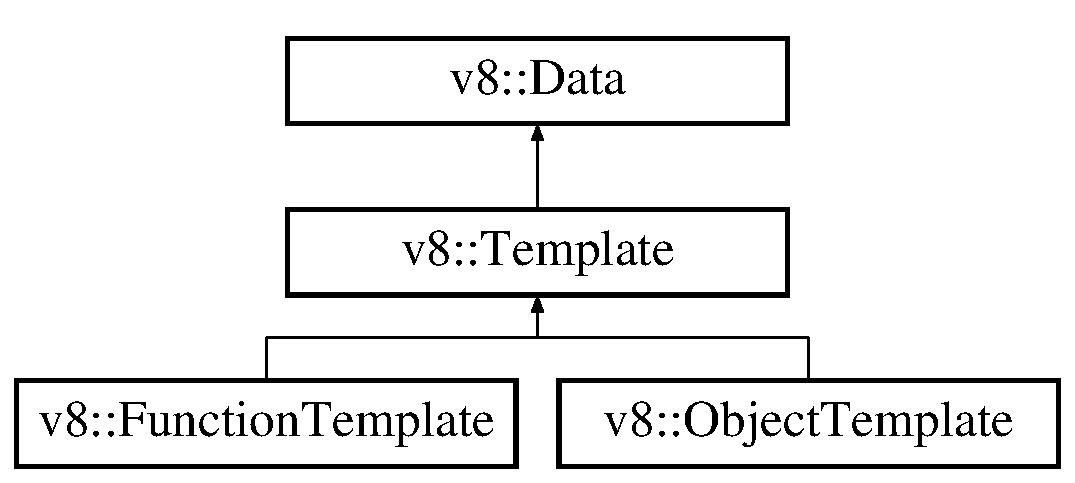
\includegraphics[height=3.000000cm]{classv8_1_1_template}
\end{center}
\end{figure}
\subsection*{Public Member Functions}
\begin{DoxyCompactItemize}
\item 
void \hyperlink{classv8_1_1_template_a8a29557db5d0bc980752084b925a9b01}{Set} (\hyperlink{classv8_1_1_handle}{Handle}$<$ \hyperlink{classv8_1_1_string}{String} $>$ name, \hyperlink{classv8_1_1_handle}{Handle}$<$ \hyperlink{classv8_1_1_data}{Data} $>$ value, Property\+Attribute attributes=None)
\item 
\hypertarget{classv8_1_1_template_a2efda45d51b493bd30f254941b7c8310}{}V8\+\_\+\+I\+N\+L\+I\+N\+E void {\bfseries Set} (const char $\ast$name, \hyperlink{classv8_1_1_handle}{Handle}$<$ \hyperlink{classv8_1_1_data}{Data} $>$ value)\label{classv8_1_1_template_a2efda45d51b493bd30f254941b7c8310}

\item 
\hypertarget{classv8_1_1_template_a1806da8c927107645490f72780f7da8c}{}void {\bfseries Set\+Accessor\+Property} (\hyperlink{classv8_1_1_local}{Local}$<$ \hyperlink{classv8_1_1_string}{String} $>$ name, \hyperlink{classv8_1_1_local}{Local}$<$ \hyperlink{classv8_1_1_function_template}{Function\+Template} $>$ getter=\hyperlink{classv8_1_1_local}{Local}$<$ \hyperlink{classv8_1_1_function_template}{Function\+Template} $>$(), \hyperlink{classv8_1_1_local}{Local}$<$ \hyperlink{classv8_1_1_function_template}{Function\+Template} $>$ setter=\hyperlink{classv8_1_1_local}{Local}$<$ \hyperlink{classv8_1_1_function_template}{Function\+Template} $>$(), Property\+Attribute attribute=None, \hyperlink{namespacev8_a31d8355cb043d7d2dda3f4a52760b64e}{Access\+Control} settings=D\+E\+F\+A\+U\+L\+T)\label{classv8_1_1_template_a1806da8c927107645490f72780f7da8c}

\item 
void \hyperlink{classv8_1_1_template_ae186b9e472ed7604cc9693c7b9540909}{Set\+Native\+Data\+Property} (\hyperlink{classv8_1_1_local}{Local}$<$ \hyperlink{classv8_1_1_string}{String} $>$ name, \hyperlink{namespacev8_a722613c87061708a4f1aa050d095f868}{Accessor\+Getter\+Callback} getter, Accessor\+Setter\+Callback setter=0, \hyperlink{classv8_1_1_handle}{Handle}$<$ \hyperlink{classv8_1_1_value}{Value} $>$ data=\hyperlink{classv8_1_1_handle}{Handle}$<$ \hyperlink{classv8_1_1_value}{Value} $>$(), Property\+Attribute attribute=None, \hyperlink{classv8_1_1_local}{Local}$<$ \hyperlink{classv8_1_1_accessor_signature}{Accessor\+Signature} $>$ signature=\hyperlink{classv8_1_1_local}{Local}$<$ \hyperlink{classv8_1_1_accessor_signature}{Accessor\+Signature} $>$(), \hyperlink{namespacev8_a31d8355cb043d7d2dda3f4a52760b64e}{Access\+Control} settings=D\+E\+F\+A\+U\+L\+T)
\item 
\hypertarget{classv8_1_1_template_a82a06b2a76a32883f2f756a919b2dee8}{}bool {\bfseries Set\+Declared\+Accessor} (\hyperlink{classv8_1_1_local}{Local}$<$ \hyperlink{classv8_1_1_string}{String} $>$ name, \hyperlink{classv8_1_1_local}{Local}$<$ \hyperlink{classv8_1_1_declared_accessor_descriptor}{Declared\+Accessor\+Descriptor} $>$ descriptor, Property\+Attribute attribute=None, \hyperlink{classv8_1_1_local}{Local}$<$ \hyperlink{classv8_1_1_accessor_signature}{Accessor\+Signature} $>$ signature=\hyperlink{classv8_1_1_local}{Local}$<$ \hyperlink{classv8_1_1_accessor_signature}{Accessor\+Signature} $>$(), \hyperlink{namespacev8_a31d8355cb043d7d2dda3f4a52760b64e}{Access\+Control} settings=D\+E\+F\+A\+U\+L\+T)\label{classv8_1_1_template_a82a06b2a76a32883f2f756a919b2dee8}

\end{DoxyCompactItemize}
\subsection*{Friends}
\begin{DoxyCompactItemize}
\item 
\hypertarget{classv8_1_1_template_a4d28646409234f556983be8a96c06424}{}class {\bfseries Object\+Template}\label{classv8_1_1_template_a4d28646409234f556983be8a96c06424}

\item 
\hypertarget{classv8_1_1_template_a334168ad1a5f39cf17b818ca3356aacd}{}class {\bfseries Function\+Template}\label{classv8_1_1_template_a334168ad1a5f39cf17b818ca3356aacd}

\end{DoxyCompactItemize}


\subsection{Detailed Description}
The superclass of object and function templates. 

\subsection{Member Function Documentation}
\hypertarget{classv8_1_1_template_a8a29557db5d0bc980752084b925a9b01}{}\index{v8\+::\+Template@{v8\+::\+Template}!Set@{Set}}
\index{Set@{Set}!v8\+::\+Template@{v8\+::\+Template}}
\subsubsection[{Set}]{\setlength{\rightskip}{0pt plus 5cm}void v8\+::\+Template\+::\+Set (
\begin{DoxyParamCaption}
\item[{{\bf Handle}$<$ {\bf String} $>$}]{name, }
\item[{{\bf Handle}$<$ {\bf Data} $>$}]{value, }
\item[{Property\+Attribute}]{attributes = {\ttfamily None}}
\end{DoxyParamCaption}
)}\label{classv8_1_1_template_a8a29557db5d0bc980752084b925a9b01}
Adds a property to each instance created by this template. \hypertarget{classv8_1_1_template_ae186b9e472ed7604cc9693c7b9540909}{}\index{v8\+::\+Template@{v8\+::\+Template}!Set\+Native\+Data\+Property@{Set\+Native\+Data\+Property}}
\index{Set\+Native\+Data\+Property@{Set\+Native\+Data\+Property}!v8\+::\+Template@{v8\+::\+Template}}
\subsubsection[{Set\+Native\+Data\+Property}]{\setlength{\rightskip}{0pt plus 5cm}void v8\+::\+Template\+::\+Set\+Native\+Data\+Property (
\begin{DoxyParamCaption}
\item[{{\bf Local}$<$ {\bf String} $>$}]{name, }
\item[{{\bf Accessor\+Getter\+Callback}}]{getter, }
\item[{Accessor\+Setter\+Callback}]{setter = {\ttfamily 0}, }
\item[{{\bf Handle}$<$ {\bf Value} $>$}]{data = {\ttfamily {\bf Handle}$<$~{\bf Value}~$>$()}, }
\item[{Property\+Attribute}]{attribute = {\ttfamily None}, }
\item[{{\bf Local}$<$ {\bf Accessor\+Signature} $>$}]{signature = {\ttfamily {\bf Local}$<$~{\bf Accessor\+Signature}~$>$()}, }
\item[{{\bf Access\+Control}}]{settings = {\ttfamily DEFAULT}}
\end{DoxyParamCaption}
)}\label{classv8_1_1_template_ae186b9e472ed7604cc9693c7b9540909}
Whenever the property with the given name is accessed on objects created from this \hyperlink{classv8_1_1_template}{Template} the getter and setter callbacks are called instead of getting and setting the property directly on the Java\+Script object.


\begin{DoxyParams}{Parameters}
{\em name} & The name of the property for which an accessor is added. \\
\hline
{\em getter} & The callback to invoke when getting the property. \\
\hline
{\em setter} & The callback to invoke when setting the property. \\
\hline
{\em data} & A piece of data that will be passed to the getter and setter callbacks whenever they are invoked. \\
\hline
{\em settings} & Access control settings for the accessor. This is a bit field consisting of one of more of D\+E\+F\+A\+U\+L\+T = 0, A\+L\+L\+\_\+\+C\+A\+N\+\_\+\+R\+E\+A\+D = 1, or A\+L\+L\+\_\+\+C\+A\+N\+\_\+\+W\+R\+I\+T\+E = 2. The default is to not allow cross-\/context access. A\+L\+L\+\_\+\+C\+A\+N\+\_\+\+R\+E\+A\+D means that all cross-\/context reads are allowed. A\+L\+L\+\_\+\+C\+A\+N\+\_\+\+W\+R\+I\+T\+E means that all cross-\/context writes are allowed. The combination A\+L\+L\+\_\+\+C\+A\+N\+\_\+\+R\+E\+A\+D $\vert$ A\+L\+L\+\_\+\+C\+A\+N\+\_\+\+W\+R\+I\+T\+E can be used to allow all cross-\/context access. \\
\hline
{\em attribute} & The attributes of the property for which an accessor is added. \\
\hline
{\em signature} & The signature describes valid receivers for the accessor and is used to perform implicit instance checks against them. If the receiver is incompatible (i.\+e. is not an instance of the constructor as defined by \hyperlink{classv8_1_1_function_template_aa883e4ab6643498662f7873506098c98}{Function\+Template\+::\+Has\+Instance()}), an implicit Type\+Error is thrown and no callback is invoked. \\
\hline
\end{DoxyParams}


The documentation for this class was generated from the following file\+:\begin{DoxyCompactItemize}
\item 
deps/v8/include/v8.\+h\end{DoxyCompactItemize}

\hypertarget{classv8_1_1_testing}{}\section{v8\+:\+:Testing Class Reference}
\label{classv8_1_1_testing}\index{v8\+::\+Testing@{v8\+::\+Testing}}
\subsection*{Public Types}
\begin{DoxyCompactItemize}
\item 
\hypertarget{classv8_1_1_testing_a436a1a521a0bc070cc0b46ad7a658575}{}enum {\bfseries Stress\+Type} \{ {\bfseries k\+Stress\+Type\+Opt}, 
{\bfseries k\+Stress\+Type\+Deopt}
 \}\label{classv8_1_1_testing_a436a1a521a0bc070cc0b46ad7a658575}

\end{DoxyCompactItemize}
\subsection*{Static Public Member Functions}
\begin{DoxyCompactItemize}
\item 
static void \hyperlink{classv8_1_1_testing_aafa5a4917998aa64134aa750ce5c4b2e}{Set\+Stress\+Run\+Type} (Stress\+Type type)
\item 
static int \hyperlink{classv8_1_1_testing_adc876063b1e07462b8d9544dd8efab36}{Get\+Stress\+Runs} ()
\item 
static void \hyperlink{classv8_1_1_testing_ab9da044b18b9d05770b655bed27ed7f4}{Prepare\+Stress\+Run} (int run)
\item 
static void \hyperlink{classv8_1_1_testing_ae541bd8d75667db1d83c8aef7f8c1cf3}{Deoptimize\+All} ()
\end{DoxyCompactItemize}


\subsection{Member Function Documentation}
\hypertarget{classv8_1_1_testing_ae541bd8d75667db1d83c8aef7f8c1cf3}{}\index{v8\+::\+Testing@{v8\+::\+Testing}!Deoptimize\+All@{Deoptimize\+All}}
\index{Deoptimize\+All@{Deoptimize\+All}!v8\+::\+Testing@{v8\+::\+Testing}}
\subsubsection[{Deoptimize\+All}]{\setlength{\rightskip}{0pt plus 5cm}static void v8\+::\+Testing\+::\+Deoptimize\+All (
\begin{DoxyParamCaption}
{}
\end{DoxyParamCaption}
)\hspace{0.3cm}{\ttfamily [static]}}\label{classv8_1_1_testing_ae541bd8d75667db1d83c8aef7f8c1cf3}
Force deoptimization of all functions. \hypertarget{classv8_1_1_testing_adc876063b1e07462b8d9544dd8efab36}{}\index{v8\+::\+Testing@{v8\+::\+Testing}!Get\+Stress\+Runs@{Get\+Stress\+Runs}}
\index{Get\+Stress\+Runs@{Get\+Stress\+Runs}!v8\+::\+Testing@{v8\+::\+Testing}}
\subsubsection[{Get\+Stress\+Runs}]{\setlength{\rightskip}{0pt plus 5cm}static int v8\+::\+Testing\+::\+Get\+Stress\+Runs (
\begin{DoxyParamCaption}
{}
\end{DoxyParamCaption}
)\hspace{0.3cm}{\ttfamily [static]}}\label{classv8_1_1_testing_adc876063b1e07462b8d9544dd8efab36}
Get the number of runs of a given test that is required to get the full stress coverage. \hypertarget{classv8_1_1_testing_ab9da044b18b9d05770b655bed27ed7f4}{}\index{v8\+::\+Testing@{v8\+::\+Testing}!Prepare\+Stress\+Run@{Prepare\+Stress\+Run}}
\index{Prepare\+Stress\+Run@{Prepare\+Stress\+Run}!v8\+::\+Testing@{v8\+::\+Testing}}
\subsubsection[{Prepare\+Stress\+Run}]{\setlength{\rightskip}{0pt plus 5cm}static void v8\+::\+Testing\+::\+Prepare\+Stress\+Run (
\begin{DoxyParamCaption}
\item[{int}]{run}
\end{DoxyParamCaption}
)\hspace{0.3cm}{\ttfamily [static]}}\label{classv8_1_1_testing_ab9da044b18b9d05770b655bed27ed7f4}
Indicate the number of the run which is about to start. The value of run should be between 0 and one less than the result from \hyperlink{classv8_1_1_testing_adc876063b1e07462b8d9544dd8efab36}{Get\+Stress\+Runs()} \hypertarget{classv8_1_1_testing_aafa5a4917998aa64134aa750ce5c4b2e}{}\index{v8\+::\+Testing@{v8\+::\+Testing}!Set\+Stress\+Run\+Type@{Set\+Stress\+Run\+Type}}
\index{Set\+Stress\+Run\+Type@{Set\+Stress\+Run\+Type}!v8\+::\+Testing@{v8\+::\+Testing}}
\subsubsection[{Set\+Stress\+Run\+Type}]{\setlength{\rightskip}{0pt plus 5cm}static void v8\+::\+Testing\+::\+Set\+Stress\+Run\+Type (
\begin{DoxyParamCaption}
\item[{Stress\+Type}]{type}
\end{DoxyParamCaption}
)\hspace{0.3cm}{\ttfamily [static]}}\label{classv8_1_1_testing_aafa5a4917998aa64134aa750ce5c4b2e}
Set the type of stressing to do. The default if not set is k\+Stress\+Type\+Opt. 

The documentation for this class was generated from the following file\+:\begin{DoxyCompactItemize}
\item 
deps/v8/include/v8-\/testing.\+h\end{DoxyCompactItemize}

\hypertarget{classv8_1_1_try_catch}{}\section{v8\+:\+:Try\+Catch Class Reference}
\label{classv8_1_1_try_catch}\index{v8\+::\+Try\+Catch@{v8\+::\+Try\+Catch}}


{\ttfamily \#include $<$v8.\+h$>$}

\subsection*{Public Member Functions}
\begin{DoxyCompactItemize}
\item 
\hyperlink{classv8_1_1_try_catch_ae3b6a2248b687b2cbc5271fcc2e40d66}{V8\+\_\+\+D\+E\+P\+R\+E\+C\+A\+T\+E\+\_\+\+S\+O\+O\+N} (\char`\"{}Use isolate version\char`\"{}, Try\+Catch())
\item 
\hyperlink{classv8_1_1_try_catch_a623ce624491b383fae60c05d2aeefb1a}{Try\+Catch} (\hyperlink{classv8_1_1_isolate}{Isolate} $\ast$isolate)
\item 
\hyperlink{classv8_1_1_try_catch_a2c9ad4b40d17dd31c6dd020736b30679}{$\sim$\+Try\+Catch} ()
\item 
bool \hyperlink{classv8_1_1_try_catch_a48f704fbf2b82564b5d2a4ff596e4137}{Has\+Caught} () const 
\item 
bool \hyperlink{classv8_1_1_try_catch_a2ec467d4653d26c064d749cab98791cb}{Can\+Continue} () const 
\item 
bool \hyperlink{classv8_1_1_try_catch_a7e012477ac47db9480f85d55427987c7}{Has\+Terminated} () const 
\item 
\hyperlink{classv8_1_1_local}{Handle}$<$ \hyperlink{classv8_1_1_value}{Value} $>$ \hyperlink{classv8_1_1_try_catch_a4a7506617800bbc49c3c08bbfefb9c2d}{Re\+Throw} ()
\item 
\hyperlink{classv8_1_1_local}{Local}$<$ \hyperlink{classv8_1_1_value}{Value} $>$ \hyperlink{classv8_1_1_try_catch_a99c425f29b3355b4294cbe762377f99b}{Exception} () const 
\item 
\hyperlink{classv8_1_1_try_catch_ae8128ec2dae652a47c545d775c7778f7}{V8\+\_\+\+D\+E\+P\+R\+E\+C\+A\+T\+E\+\_\+\+S\+O\+O\+N} (\char`\"{}Use maybe version.\char`\"{}, Local$<$ \hyperlink{classv8_1_1_value}{Value} $>$ \hyperlink{classv8_1_1_stack_trace}{Stack\+Trace}()) const 
\item 
\hypertarget{classv8_1_1_try_catch_a449fe4cdc063d234f2bea39e9297ba28}{}V8\+\_\+\+W\+A\+R\+N\+\_\+\+U\+N\+U\+S\+E\+D\+\_\+\+R\+E\+S\+U\+L\+T \hyperlink{classv8_1_1_maybe_local}{Maybe\+Local}$<$ \hyperlink{classv8_1_1_value}{Value} $>$ {\bfseries Stack\+Trace} (\hyperlink{classv8_1_1_local}{Local}$<$ \hyperlink{classv8_1_1_context}{Context} $>$ context) const \label{classv8_1_1_try_catch_a449fe4cdc063d234f2bea39e9297ba28}

\item 
\hyperlink{classv8_1_1_local}{Local}$<$ \hyperlink{classv8_1_1_message}{v8\+::\+Message} $>$ \hyperlink{classv8_1_1_try_catch_a2811e500fbb906ee505895a3d94fc66f}{Message} () const 
\item 
void \hyperlink{classv8_1_1_try_catch_a3aae8acab4c99b374b7d782763d4c8e1}{Reset} ()
\item 
void \hyperlink{classv8_1_1_try_catch_a032cd889d76bd596e2616df11ced8682}{Set\+Verbose} (bool value)
\item 
void \hyperlink{classv8_1_1_try_catch_a541b8fa6951bd5a439692c22d5c7b73c}{Set\+Capture\+Message} (bool value)
\end{DoxyCompactItemize}
\subsection*{Static Public Member Functions}
\begin{DoxyCompactItemize}
\item 
static void $\ast$ \hyperlink{classv8_1_1_try_catch_ac2e6359fa11a2aba609af82fb80cf07a}{J\+S\+Stack\+Comparable\+Address} (\hyperlink{classv8_1_1_try_catch}{v8\+::\+Try\+Catch} $\ast$handler)
\end{DoxyCompactItemize}
\subsection*{Friends}
\begin{DoxyCompactItemize}
\item 
\hypertarget{classv8_1_1_try_catch_acda8e558d20805fa72df899e935081aa}{}class {\bfseries v8\+::internal\+::\+Isolate}\label{classv8_1_1_try_catch_acda8e558d20805fa72df899e935081aa}

\end{DoxyCompactItemize}


\subsection{Detailed Description}
An external exception handler. 

\subsection{Constructor \& Destructor Documentation}
\hypertarget{classv8_1_1_try_catch_a623ce624491b383fae60c05d2aeefb1a}{}\index{v8\+::\+Try\+Catch@{v8\+::\+Try\+Catch}!Try\+Catch@{Try\+Catch}}
\index{Try\+Catch@{Try\+Catch}!v8\+::\+Try\+Catch@{v8\+::\+Try\+Catch}}
\subsubsection[{Try\+Catch}]{\setlength{\rightskip}{0pt plus 5cm}v8\+::\+Try\+Catch\+::\+Try\+Catch (
\begin{DoxyParamCaption}
\item[{{\bf Isolate} $\ast$}]{isolate}
\end{DoxyParamCaption}
)}\label{classv8_1_1_try_catch_a623ce624491b383fae60c05d2aeefb1a}
Creates a new try/catch block and registers it with \hyperlink{namespacev8}{v8}. Note that all \hyperlink{classv8_1_1_try_catch}{Try\+Catch} blocks should be stack allocated because the memory location itself is compared against Java\+Script try/catch blocks. \hypertarget{classv8_1_1_try_catch_a2c9ad4b40d17dd31c6dd020736b30679}{}\index{v8\+::\+Try\+Catch@{v8\+::\+Try\+Catch}!````~Try\+Catch@{$\sim$\+Try\+Catch}}
\index{````~Try\+Catch@{$\sim$\+Try\+Catch}!v8\+::\+Try\+Catch@{v8\+::\+Try\+Catch}}
\subsubsection[{$\sim$\+Try\+Catch}]{\setlength{\rightskip}{0pt plus 5cm}v8\+::\+Try\+Catch\+::$\sim$\+Try\+Catch (
\begin{DoxyParamCaption}
{}
\end{DoxyParamCaption}
)}\label{classv8_1_1_try_catch_a2c9ad4b40d17dd31c6dd020736b30679}
Unregisters and deletes this try/catch block. 

\subsection{Member Function Documentation}
\hypertarget{classv8_1_1_try_catch_a2ec467d4653d26c064d749cab98791cb}{}\index{v8\+::\+Try\+Catch@{v8\+::\+Try\+Catch}!Can\+Continue@{Can\+Continue}}
\index{Can\+Continue@{Can\+Continue}!v8\+::\+Try\+Catch@{v8\+::\+Try\+Catch}}
\subsubsection[{Can\+Continue}]{\setlength{\rightskip}{0pt plus 5cm}bool v8\+::\+Try\+Catch\+::\+Can\+Continue (
\begin{DoxyParamCaption}
{}
\end{DoxyParamCaption}
) const}\label{classv8_1_1_try_catch_a2ec467d4653d26c064d749cab98791cb}
For certain types of exceptions, it makes no sense to continue execution.

If Can\+Continue returns false, the correct action is to perform any C++ cleanup needed and then return. If Can\+Continue returns false and Has\+Terminated returns true, it is possible to call Cancel\+Terminate\+Execution in order to continue calling into the engine. \hypertarget{classv8_1_1_try_catch_a99c425f29b3355b4294cbe762377f99b}{}\index{v8\+::\+Try\+Catch@{v8\+::\+Try\+Catch}!Exception@{Exception}}
\index{Exception@{Exception}!v8\+::\+Try\+Catch@{v8\+::\+Try\+Catch}}
\subsubsection[{Exception}]{\setlength{\rightskip}{0pt plus 5cm}{\bf Local}$<${\bf Value}$>$ v8\+::\+Try\+Catch\+::\+Exception (
\begin{DoxyParamCaption}
{}
\end{DoxyParamCaption}
) const}\label{classv8_1_1_try_catch_a99c425f29b3355b4294cbe762377f99b}
Returns the exception caught by this try/catch block. If no exception has been caught an empty handle is returned.

The returned handle is valid until this \hyperlink{classv8_1_1_try_catch}{Try\+Catch} block has been destroyed. \hypertarget{classv8_1_1_try_catch_a48f704fbf2b82564b5d2a4ff596e4137}{}\index{v8\+::\+Try\+Catch@{v8\+::\+Try\+Catch}!Has\+Caught@{Has\+Caught}}
\index{Has\+Caught@{Has\+Caught}!v8\+::\+Try\+Catch@{v8\+::\+Try\+Catch}}
\subsubsection[{Has\+Caught}]{\setlength{\rightskip}{0pt plus 5cm}bool v8\+::\+Try\+Catch\+::\+Has\+Caught (
\begin{DoxyParamCaption}
{}
\end{DoxyParamCaption}
) const}\label{classv8_1_1_try_catch_a48f704fbf2b82564b5d2a4ff596e4137}
Returns true if an exception has been caught by this try/catch block. \hypertarget{classv8_1_1_try_catch_a7e012477ac47db9480f85d55427987c7}{}\index{v8\+::\+Try\+Catch@{v8\+::\+Try\+Catch}!Has\+Terminated@{Has\+Terminated}}
\index{Has\+Terminated@{Has\+Terminated}!v8\+::\+Try\+Catch@{v8\+::\+Try\+Catch}}
\subsubsection[{Has\+Terminated}]{\setlength{\rightskip}{0pt plus 5cm}bool v8\+::\+Try\+Catch\+::\+Has\+Terminated (
\begin{DoxyParamCaption}
{}
\end{DoxyParamCaption}
) const}\label{classv8_1_1_try_catch_a7e012477ac47db9480f85d55427987c7}
Returns true if an exception has been caught due to script execution being terminated.

There is no Java\+Script representation of an execution termination exception. Such exceptions are thrown when the Terminate\+Execution methods are called to terminate a long-\/running script.

If such an exception has been thrown, Has\+Terminated will return true, indicating that it is possible to call Cancel\+Terminate\+Execution in order to continue calling into the engine. \hypertarget{classv8_1_1_try_catch_ac2e6359fa11a2aba609af82fb80cf07a}{}\index{v8\+::\+Try\+Catch@{v8\+::\+Try\+Catch}!J\+S\+Stack\+Comparable\+Address@{J\+S\+Stack\+Comparable\+Address}}
\index{J\+S\+Stack\+Comparable\+Address@{J\+S\+Stack\+Comparable\+Address}!v8\+::\+Try\+Catch@{v8\+::\+Try\+Catch}}
\subsubsection[{J\+S\+Stack\+Comparable\+Address}]{\setlength{\rightskip}{0pt plus 5cm}static void$\ast$ v8\+::\+Try\+Catch\+::\+J\+S\+Stack\+Comparable\+Address (
\begin{DoxyParamCaption}
\item[{{\bf v8\+::\+Try\+Catch} $\ast$}]{handler}
\end{DoxyParamCaption}
)\hspace{0.3cm}{\ttfamily [inline]}, {\ttfamily [static]}}\label{classv8_1_1_try_catch_ac2e6359fa11a2aba609af82fb80cf07a}
There are cases when the raw address of C++ \hyperlink{classv8_1_1_try_catch}{Try\+Catch} object cannot be used for comparisons with addresses into the J\+S stack. The cases are\+: 1) A\+R\+M, A\+R\+M64 and M\+I\+P\+S simulators which have separate J\+S stack. 2) Address sanitizer allocates local C++ object in the heap when Use\+After\+Return mode is enabled. This method returns address that can be used for comparisons with addresses into the J\+S stack. When neither simulator nor A\+S\+A\+N\textquotesingle{}s Use\+After\+Return is enabled, then the address returned will be the address of the C++ try catch handler itself. \hypertarget{classv8_1_1_try_catch_a2811e500fbb906ee505895a3d94fc66f}{}\index{v8\+::\+Try\+Catch@{v8\+::\+Try\+Catch}!Message@{Message}}
\index{Message@{Message}!v8\+::\+Try\+Catch@{v8\+::\+Try\+Catch}}
\subsubsection[{Message}]{\setlength{\rightskip}{0pt plus 5cm}{\bf Local}$<${\bf v8\+::\+Message}$>$ v8\+::\+Try\+Catch\+::\+Message (
\begin{DoxyParamCaption}
{}
\end{DoxyParamCaption}
) const}\label{classv8_1_1_try_catch_a2811e500fbb906ee505895a3d94fc66f}
Returns the message associated with this exception. If there is no message associated an empty handle is returned.

The returned handle is valid until this \hyperlink{classv8_1_1_try_catch}{Try\+Catch} block has been destroyed. \hypertarget{classv8_1_1_try_catch_a3aae8acab4c99b374b7d782763d4c8e1}{}\index{v8\+::\+Try\+Catch@{v8\+::\+Try\+Catch}!Reset@{Reset}}
\index{Reset@{Reset}!v8\+::\+Try\+Catch@{v8\+::\+Try\+Catch}}
\subsubsection[{Reset}]{\setlength{\rightskip}{0pt plus 5cm}void v8\+::\+Try\+Catch\+::\+Reset (
\begin{DoxyParamCaption}
{}
\end{DoxyParamCaption}
)}\label{classv8_1_1_try_catch_a3aae8acab4c99b374b7d782763d4c8e1}
Clears any exceptions that may have been caught by this try/catch block. After this method has been called, \hyperlink{classv8_1_1_try_catch_a48f704fbf2b82564b5d2a4ff596e4137}{Has\+Caught()} will return false. Cancels the scheduled exception if it is caught and \hyperlink{classv8_1_1_try_catch_a4a7506617800bbc49c3c08bbfefb9c2d}{Re\+Throw()} is not called before.

It is not necessary to clear a try/catch block before using it again; if another exception is thrown the previously caught exception will just be overwritten. However, it is often a good idea since it makes it easier to determine which operation threw a given exception. \hypertarget{classv8_1_1_try_catch_a4a7506617800bbc49c3c08bbfefb9c2d}{}\index{v8\+::\+Try\+Catch@{v8\+::\+Try\+Catch}!Re\+Throw@{Re\+Throw}}
\index{Re\+Throw@{Re\+Throw}!v8\+::\+Try\+Catch@{v8\+::\+Try\+Catch}}
\subsubsection[{Re\+Throw}]{\setlength{\rightskip}{0pt plus 5cm}{\bf Handle}$<${\bf Value}$>$ v8\+::\+Try\+Catch\+::\+Re\+Throw (
\begin{DoxyParamCaption}
{}
\end{DoxyParamCaption}
)}\label{classv8_1_1_try_catch_a4a7506617800bbc49c3c08bbfefb9c2d}
Throws the exception caught by this \hyperlink{classv8_1_1_try_catch}{Try\+Catch} in a way that avoids it being caught again by this same \hyperlink{classv8_1_1_try_catch}{Try\+Catch}. As with Throw\+Exception it is illegal to execute any Java\+Script operations after calling Re\+Throw; the caller must return immediately to where the exception is caught. \hypertarget{classv8_1_1_try_catch_a541b8fa6951bd5a439692c22d5c7b73c}{}\index{v8\+::\+Try\+Catch@{v8\+::\+Try\+Catch}!Set\+Capture\+Message@{Set\+Capture\+Message}}
\index{Set\+Capture\+Message@{Set\+Capture\+Message}!v8\+::\+Try\+Catch@{v8\+::\+Try\+Catch}}
\subsubsection[{Set\+Capture\+Message}]{\setlength{\rightskip}{0pt plus 5cm}void v8\+::\+Try\+Catch\+::\+Set\+Capture\+Message (
\begin{DoxyParamCaption}
\item[{bool}]{value}
\end{DoxyParamCaption}
)}\label{classv8_1_1_try_catch_a541b8fa6951bd5a439692c22d5c7b73c}
Set whether or not this \hyperlink{classv8_1_1_try_catch}{Try\+Catch} should capture a \hyperlink{classv8_1_1_message}{Message} object which holds source information about where the exception occurred. True by default. \hypertarget{classv8_1_1_try_catch_a032cd889d76bd596e2616df11ced8682}{}\index{v8\+::\+Try\+Catch@{v8\+::\+Try\+Catch}!Set\+Verbose@{Set\+Verbose}}
\index{Set\+Verbose@{Set\+Verbose}!v8\+::\+Try\+Catch@{v8\+::\+Try\+Catch}}
\subsubsection[{Set\+Verbose}]{\setlength{\rightskip}{0pt plus 5cm}void v8\+::\+Try\+Catch\+::\+Set\+Verbose (
\begin{DoxyParamCaption}
\item[{bool}]{value}
\end{DoxyParamCaption}
)}\label{classv8_1_1_try_catch_a032cd889d76bd596e2616df11ced8682}
Set verbosity of the external exception handler.

By default, exceptions that are caught by an external exception handler are not reported. Call Set\+Verbose with true on an external exception handler to have exceptions caught by the handler reported as if they were not caught. \hypertarget{classv8_1_1_try_catch_ae3b6a2248b687b2cbc5271fcc2e40d66}{}\index{v8\+::\+Try\+Catch@{v8\+::\+Try\+Catch}!V8\+\_\+\+D\+E\+P\+R\+E\+C\+A\+T\+E\+\_\+\+S\+O\+O\+N@{V8\+\_\+\+D\+E\+P\+R\+E\+C\+A\+T\+E\+\_\+\+S\+O\+O\+N}}
\index{V8\+\_\+\+D\+E\+P\+R\+E\+C\+A\+T\+E\+\_\+\+S\+O\+O\+N@{V8\+\_\+\+D\+E\+P\+R\+E\+C\+A\+T\+E\+\_\+\+S\+O\+O\+N}!v8\+::\+Try\+Catch@{v8\+::\+Try\+Catch}}
\subsubsection[{V8\+\_\+\+D\+E\+P\+R\+E\+C\+A\+T\+E\+\_\+\+S\+O\+O\+N}]{\setlength{\rightskip}{0pt plus 5cm}v8\+::\+Try\+Catch\+::\+V8\+\_\+\+D\+E\+P\+R\+E\+C\+A\+T\+E\+\_\+\+S\+O\+O\+N (
\begin{DoxyParamCaption}
\item[{\char`\"{}Use isolate version\char`\"{}}]{, }
\item[{{\bf Try\+Catch}()}]{}
\end{DoxyParamCaption}
)}\label{classv8_1_1_try_catch_ae3b6a2248b687b2cbc5271fcc2e40d66}
Creates a new try/catch block and registers it with \hyperlink{namespacev8}{v8}. Note that all \hyperlink{classv8_1_1_try_catch}{Try\+Catch} blocks should be stack allocated because the memory location itself is compared against Java\+Script try/catch blocks. \hypertarget{classv8_1_1_try_catch_ae8128ec2dae652a47c545d775c7778f7}{}\index{v8\+::\+Try\+Catch@{v8\+::\+Try\+Catch}!V8\+\_\+\+D\+E\+P\+R\+E\+C\+A\+T\+E\+\_\+\+S\+O\+O\+N@{V8\+\_\+\+D\+E\+P\+R\+E\+C\+A\+T\+E\+\_\+\+S\+O\+O\+N}}
\index{V8\+\_\+\+D\+E\+P\+R\+E\+C\+A\+T\+E\+\_\+\+S\+O\+O\+N@{V8\+\_\+\+D\+E\+P\+R\+E\+C\+A\+T\+E\+\_\+\+S\+O\+O\+N}!v8\+::\+Try\+Catch@{v8\+::\+Try\+Catch}}
\subsubsection[{V8\+\_\+\+D\+E\+P\+R\+E\+C\+A\+T\+E\+\_\+\+S\+O\+O\+N}]{\setlength{\rightskip}{0pt plus 5cm}v8\+::\+Try\+Catch\+::\+V8\+\_\+\+D\+E\+P\+R\+E\+C\+A\+T\+E\+\_\+\+S\+O\+O\+N (
\begin{DoxyParamCaption}
\item[{\char`\"{}Use maybe version.\char`\"{}}]{, }
\item[{{\bf Local}$<$ {\bf Value} $>$ }]{Stack\+Trace()}
\end{DoxyParamCaption}
) const}\label{classv8_1_1_try_catch_ae8128ec2dae652a47c545d775c7778f7}
Returns the .stack property of the thrown object. If no .stack property is present an empty handle is returned. 

The documentation for this class was generated from the following file\+:\begin{DoxyCompactItemize}
\item 
deps/v8/include/v8.\+h\end{DoxyCompactItemize}

\hypertarget{classv8_1_1_type_switch}{}\section{v8\+:\+:Type\+Switch Class Reference}
\label{classv8_1_1_type_switch}\index{v8\+::\+Type\+Switch@{v8\+::\+Type\+Switch}}


{\ttfamily \#include $<$v8.\+h$>$}

Inheritance diagram for v8\+:\+:Type\+Switch\+:\begin{figure}[H]
\begin{center}
\leavevmode
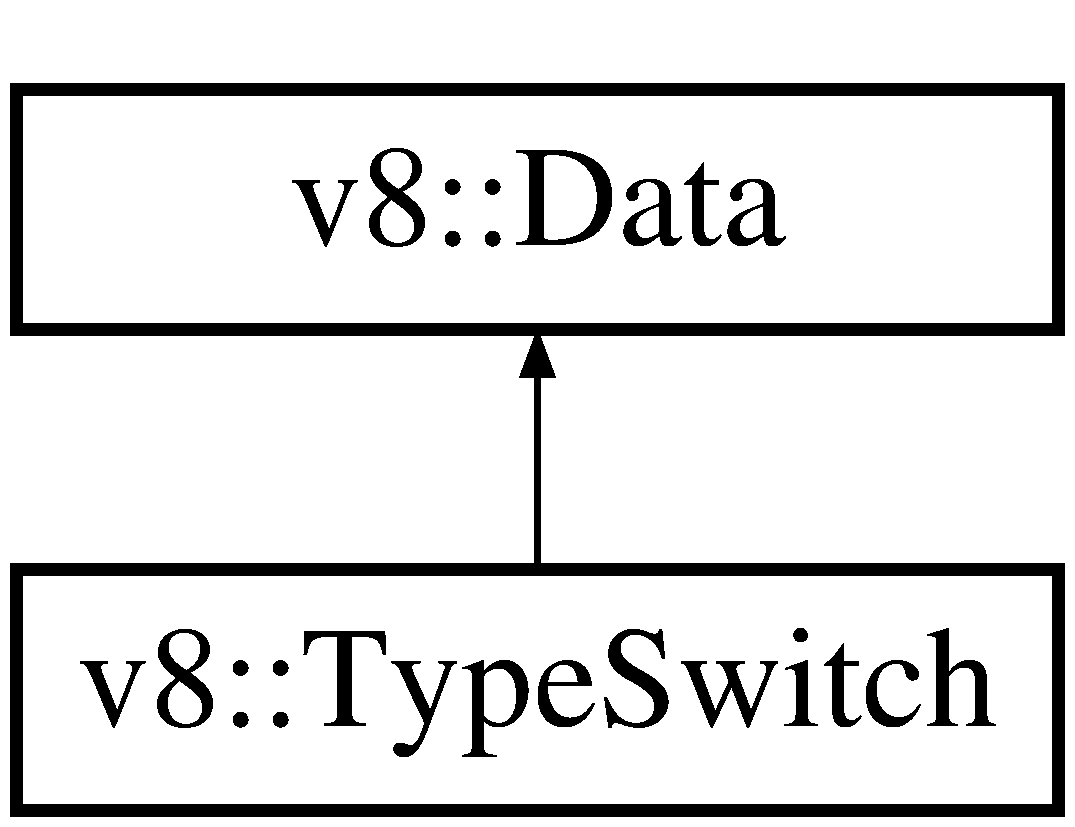
\includegraphics[height=2.000000cm]{classv8_1_1_type_switch}
\end{center}
\end{figure}
\subsection*{Public Member Functions}
\begin{DoxyCompactItemize}
\item 
\hypertarget{classv8_1_1_type_switch_a678fe45db1e97ba46df7359b51752483}{}int {\bfseries match} (\hyperlink{classv8_1_1_handle}{Handle}$<$ \hyperlink{classv8_1_1_value}{Value} $>$ value)\label{classv8_1_1_type_switch_a678fe45db1e97ba46df7359b51752483}

\end{DoxyCompactItemize}
\subsection*{Static Public Member Functions}
\begin{DoxyCompactItemize}
\item 
\hypertarget{classv8_1_1_type_switch_ac94aac0b1ba0bde763bc8b6ae6aea532}{}static \hyperlink{classv8_1_1_local}{Local}$<$ \hyperlink{classv8_1_1_type_switch}{Type\+Switch} $>$ {\bfseries New} (\hyperlink{classv8_1_1_handle}{Handle}$<$ \hyperlink{classv8_1_1_function_template}{Function\+Template} $>$ type)\label{classv8_1_1_type_switch_ac94aac0b1ba0bde763bc8b6ae6aea532}

\item 
\hypertarget{classv8_1_1_type_switch_a47003915e553a7ca2285b8a0bf42993b}{}static \hyperlink{classv8_1_1_local}{Local}$<$ \hyperlink{classv8_1_1_type_switch}{Type\+Switch} $>$ {\bfseries New} (int argc, \hyperlink{classv8_1_1_handle}{Handle}$<$ \hyperlink{classv8_1_1_function_template}{Function\+Template} $>$ types\mbox{[}$\,$\mbox{]})\label{classv8_1_1_type_switch_a47003915e553a7ca2285b8a0bf42993b}

\end{DoxyCompactItemize}


\subsection{Detailed Description}
A utility for determining the type of objects based on the template they were constructed from. 

The documentation for this class was generated from the following file\+:\begin{DoxyCompactItemize}
\item 
deps/v8/include/v8.\+h\end{DoxyCompactItemize}

\hypertarget{classv8_1_1_uint32}{}\section{v8\+:\+:Uint32 Class Reference}
\label{classv8_1_1_uint32}\index{v8\+::\+Uint32@{v8\+::\+Uint32}}


{\ttfamily \#include $<$v8.\+h$>$}

Inheritance diagram for v8\+:\+:Uint32\+:\begin{figure}[H]
\begin{center}
\leavevmode
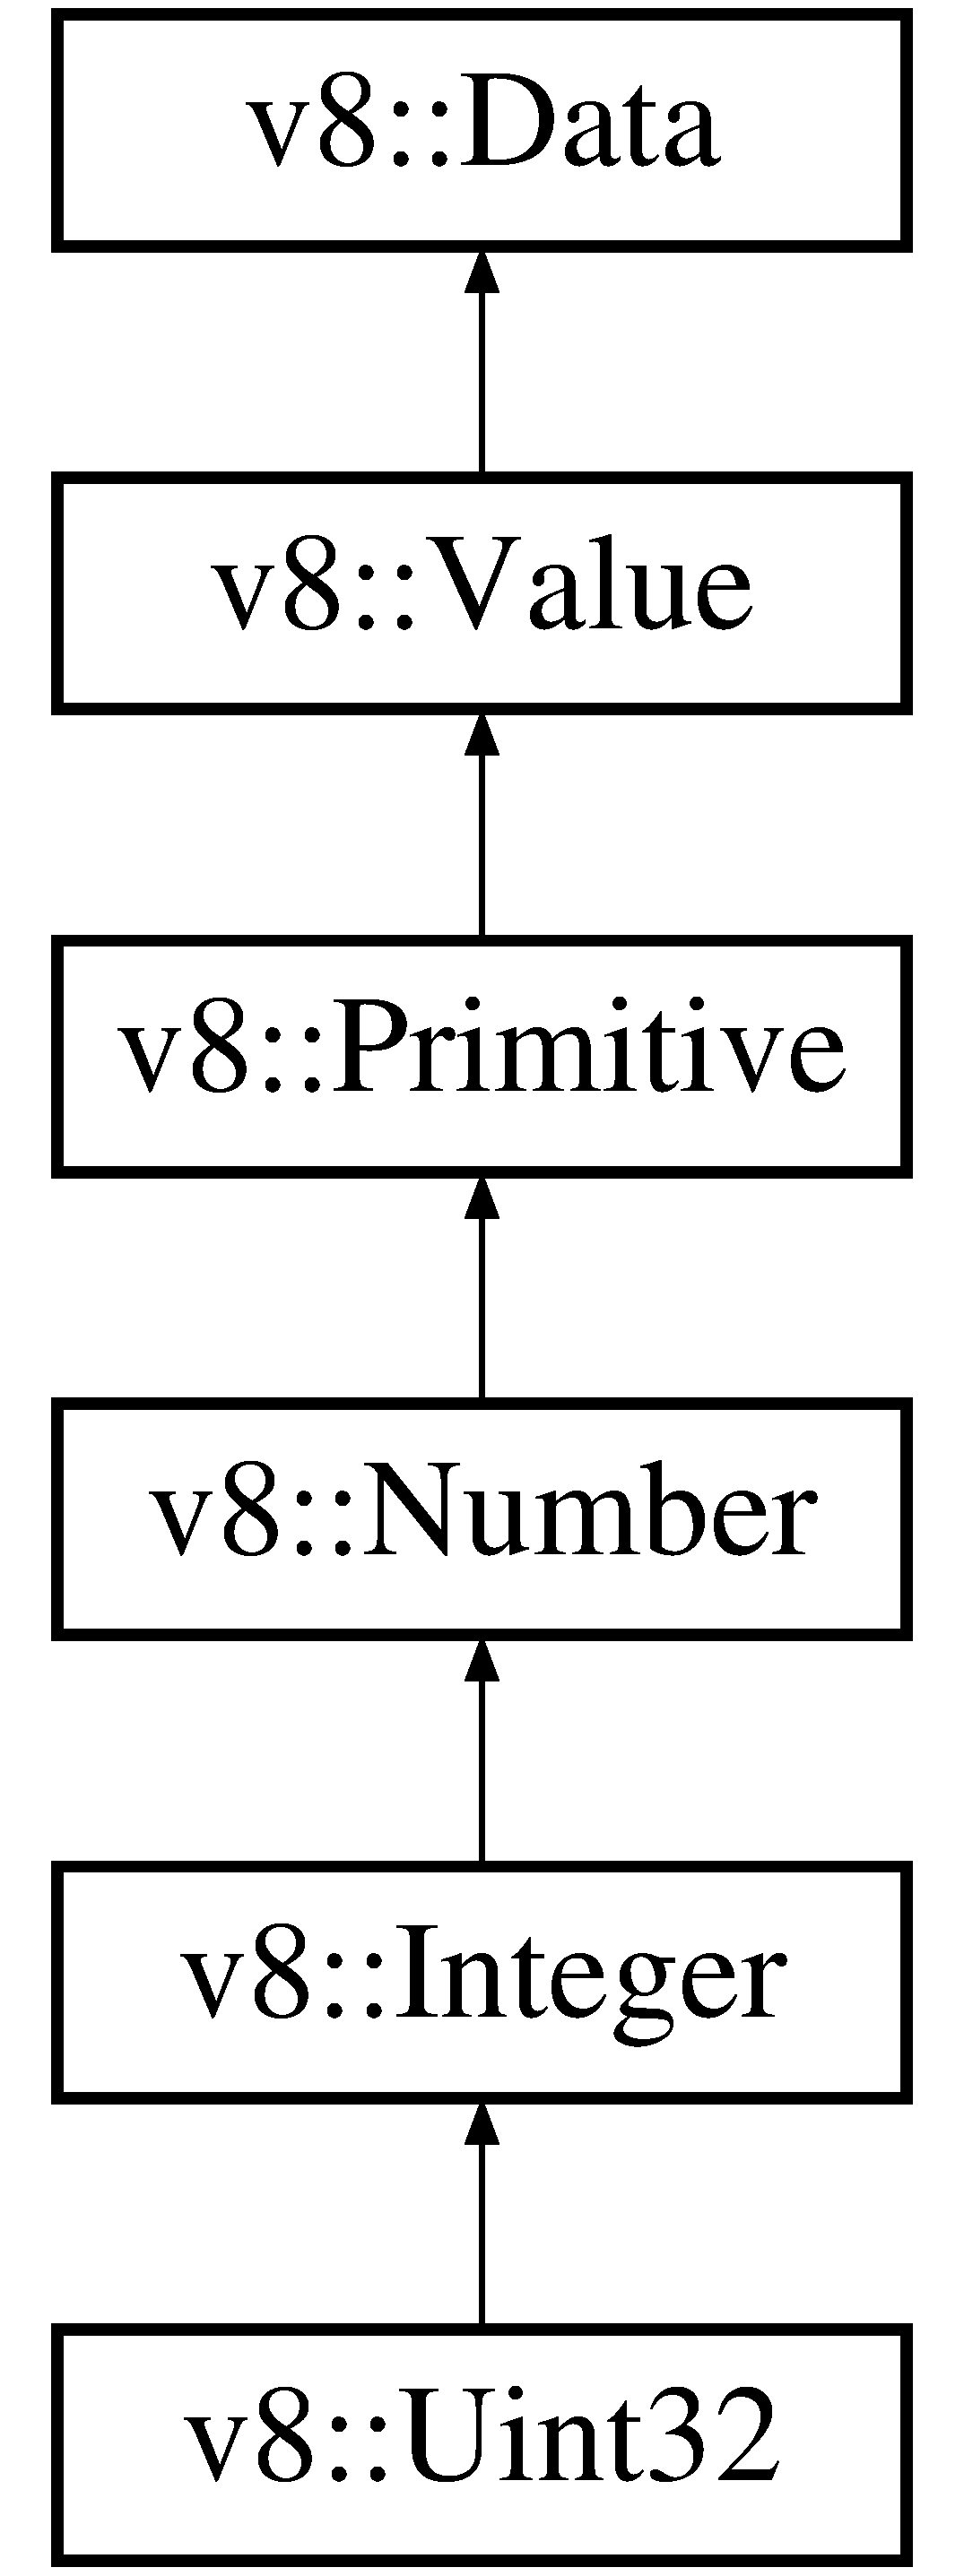
\includegraphics[height=6.000000cm]{classv8_1_1_uint32}
\end{center}
\end{figure}
\subsection*{Public Member Functions}
\begin{DoxyCompactItemize}
\item 
\hypertarget{classv8_1_1_uint32_ad59790c380f4de98c4cc479140812fe0}{}uint32\+\_\+t {\bfseries Value} () const \label{classv8_1_1_uint32_ad59790c380f4de98c4cc479140812fe0}

\end{DoxyCompactItemize}
\subsection*{Static Public Member Functions}
\begin{DoxyCompactItemize}
\item 
\hypertarget{classv8_1_1_uint32_a41a1785c19221868e338b93faa383b62}{}static V8\+\_\+\+I\+N\+L\+I\+N\+E \hyperlink{classv8_1_1_uint32}{Uint32} $\ast$ {\bfseries Cast} (\hyperlink{classv8_1_1_value}{v8\+::\+Value} $\ast$obj)\label{classv8_1_1_uint32_a41a1785c19221868e338b93faa383b62}

\end{DoxyCompactItemize}


\subsection{Detailed Description}
A Java\+Script value representing a 32-\/bit unsigned integer. 

The documentation for this class was generated from the following file\+:\begin{DoxyCompactItemize}
\item 
deps/v8/include/v8.\+h\end{DoxyCompactItemize}

\hypertarget{classv8_1_1_unicode_input_stream}{}\section{v8\+:\+:Unicode\+Input\+Stream Class Reference}
\label{classv8_1_1_unicode_input_stream}\index{v8\+::\+Unicode\+Input\+Stream@{v8\+::\+Unicode\+Input\+Stream}}
\subsection*{Public Member Functions}
\begin{DoxyCompactItemize}
\item 
\hypertarget{classv8_1_1_unicode_input_stream_a040b55d2dc511c4b2a96c7f530cd4f98}{}virtual int32\+\_\+t {\bfseries Next} ()=0\label{classv8_1_1_unicode_input_stream_a040b55d2dc511c4b2a96c7f530cd4f98}

\end{DoxyCompactItemize}


The documentation for this class was generated from the following file\+:\begin{DoxyCompactItemize}
\item 
deps/v8/include/v8-\/preparser.\+h\end{DoxyCompactItemize}

\hypertarget{classv8_1_1_unlocker}{}\section{v8\+:\+:Unlocker Class Reference}
\label{classv8_1_1_unlocker}\index{v8\+::\+Unlocker@{v8\+::\+Unlocker}}


{\ttfamily \#include $<$v8.\+h$>$}

\subsection*{Public Member Functions}
\begin{DoxyCompactItemize}
\item 
\hyperlink{classv8_1_1_unlocker_a1512a9d4ecd680f2176fea176052256f}{Unlocker} (\hyperlink{classv8_1_1_isolate}{Isolate} $\ast$isolate=N\+U\+L\+L)
\end{DoxyCompactItemize}


\subsection{Detailed Description}
Multiple threads in \hyperlink{classv8_1_1_v8}{V8} are allowed, but only one thread at a time is allowed to use any given \hyperlink{classv8_1_1_v8}{V8} isolate. See \hyperlink{classv8_1_1_isolate}{Isolate} class comments. The definition of \textquotesingle{}using \hyperlink{classv8_1_1_v8}{V8} isolate\textquotesingle{} includes accessing handles or holding onto object pointers obtained from \hyperlink{classv8_1_1_v8}{V8} handles while in the particular \hyperlink{classv8_1_1_v8}{V8} isolate. It is up to the user of \hyperlink{classv8_1_1_v8}{V8} to ensure (perhaps with locking) that this constraint is not violated.

\hyperlink{classv8_1_1_locker}{v8\+::\+Locker} is a scoped lock object. While it\textquotesingle{}s active (i.\+e. between its construction and destruction) the current thread is allowed to use the locked isolate. \hyperlink{classv8_1_1_v8}{V8} guarantees that an isolate can be locked by at most one thread at any time. In other words, the scope of a \hyperlink{classv8_1_1_locker}{v8\+::\+Locker} is a critical section.

Sample usage\+: 
\begin{DoxyCode}
...
\{
  \hyperlink{classv8_1_1_locker}{v8::Locker} locker(isolate);
  \hyperlink{classv8_1_1_isolate_1_1_scope}{v8::Isolate::Scope} isolate\_scope(isolate);
  ...
  \textcolor{comment}{// Code using V8 and isolate goes here.}
  ...
\} \textcolor{comment}{// Destructor called here}
\end{DoxyCode}


If you wish to stop using \hyperlink{classv8_1_1_v8}{V8} in a thread A you can do this either by destroying the \hyperlink{classv8_1_1_locker}{v8\+::\+Locker} object as above or by constructing a \hyperlink{classv8_1_1_unlocker}{v8\+::\+Unlocker} object\+:


\begin{DoxyCode}
\{
  isolate->Exit();
  \hyperlink{classv8_1_1_unlocker}{v8::Unlocker} unlocker(isolate);
  ...
  \textcolor{comment}{// Code not using V8 goes here while V8 can run in another thread.}
  ...
\} \textcolor{comment}{// Destructor called here.}
isolate->Enter();
\end{DoxyCode}


The \hyperlink{classv8_1_1_unlocker}{Unlocker} object is intended for use in a long-\/running callback from \hyperlink{classv8_1_1_v8}{V8}, where you want to release the \hyperlink{classv8_1_1_v8}{V8} lock for other threads to use.

The \hyperlink{classv8_1_1_locker}{v8\+::\+Locker} is a recursive lock. That is, you can lock more than once in a given thread. This can be useful if you have code that can be called either from code that holds the lock or from code that does not. The \hyperlink{classv8_1_1_unlocker}{Unlocker} is not recursive so you can not have several Unlockers on the stack at once, and you can not use an \hyperlink{classv8_1_1_unlocker}{Unlocker} in a thread that is not inside a \hyperlink{classv8_1_1_locker}{Locker}\textquotesingle{}s scope.

An unlocker will unlock several lockers if it has to and reinstate the correct depth of locking on its destruction. eg.\+:


\begin{DoxyCode}
\textcolor{comment}{// V8 not locked.}
\{
  \hyperlink{classv8_1_1_locker}{v8::Locker} locker(isolate);
  Isolate::Scope isolate\_scope(isolate);
  \textcolor{comment}{// V8 locked.}
  \{
    \hyperlink{classv8_1_1_locker}{v8::Locker} another\_locker(isolate);
    \textcolor{comment}{// V8 still locked (2 levels).}
    \{
      isolate->Exit();
      \hyperlink{classv8_1_1_unlocker}{v8::Unlocker} unlocker(isolate);
      \textcolor{comment}{// V8 not locked.}
    \}
    isolate->Enter();
    \textcolor{comment}{// V8 locked again (2 levels).}
  \}
  \textcolor{comment}{// V8 still locked (1 level).}
\}
\textcolor{comment}{// V8 Now no longer locked.}
\end{DoxyCode}
 

\subsection{Constructor \& Destructor Documentation}
\hypertarget{classv8_1_1_unlocker_a1512a9d4ecd680f2176fea176052256f}{}\index{v8\+::\+Unlocker@{v8\+::\+Unlocker}!Unlocker@{Unlocker}}
\index{Unlocker@{Unlocker}!v8\+::\+Unlocker@{v8\+::\+Unlocker}}
\subsubsection[{Unlocker}]{\setlength{\rightskip}{0pt plus 5cm}v8\+::\+Unlocker\+::\+Unlocker (
\begin{DoxyParamCaption}
\item[{{\bf Isolate} $\ast$}]{isolate = {\ttfamily NULL}}
\end{DoxyParamCaption}
)\hspace{0.3cm}{\ttfamily [explicit]}}\label{classv8_1_1_unlocker_a1512a9d4ecd680f2176fea176052256f}
Initialize \hyperlink{classv8_1_1_unlocker}{Unlocker} for a given \hyperlink{classv8_1_1_isolate}{Isolate}. N\+U\+L\+L means default isolate. 

The documentation for this class was generated from the following file\+:\begin{DoxyCompactItemize}
\item 
deps/v8/include/v8.\+h\end{DoxyCompactItemize}

\hypertarget{classv8_1_1_string_1_1_utf8_value}{}\section{v8\+:\+:String\+:\+:Utf8\+Value Class Reference}
\label{classv8_1_1_string_1_1_utf8_value}\index{v8\+::\+String\+::\+Utf8\+Value@{v8\+::\+String\+::\+Utf8\+Value}}


{\ttfamily \#include $<$v8.\+h$>$}

\subsection*{Public Member Functions}
\begin{DoxyCompactItemize}
\item 
\hypertarget{classv8_1_1_string_1_1_utf8_value_aded9fd7ed406e79d5bc40eca15b6b3d7}{}{\bfseries Utf8\+Value} (\hyperlink{classv8_1_1_local}{Handle}$<$ \hyperlink{classv8_1_1_value}{v8\+::\+Value} $>$ obj)\label{classv8_1_1_string_1_1_utf8_value_aded9fd7ed406e79d5bc40eca15b6b3d7}

\item 
\hypertarget{classv8_1_1_string_1_1_utf8_value_a6cb4914bc426bbe60b0dfdff32213e59}{}char $\ast$ {\bfseries operator$\ast$} ()\label{classv8_1_1_string_1_1_utf8_value_a6cb4914bc426bbe60b0dfdff32213e59}

\item 
\hypertarget{classv8_1_1_string_1_1_utf8_value_a6557ad0916c472faebd8bfdc3da5c4f7}{}const char $\ast$ {\bfseries operator$\ast$} () const \label{classv8_1_1_string_1_1_utf8_value_a6557ad0916c472faebd8bfdc3da5c4f7}

\item 
\hypertarget{classv8_1_1_string_1_1_utf8_value_a1e2572abf6adc0786769482df9906f19}{}int {\bfseries length} () const \label{classv8_1_1_string_1_1_utf8_value_a1e2572abf6adc0786769482df9906f19}

\end{DoxyCompactItemize}


\subsection{Detailed Description}
Converts an object to a U\+T\+F-\/8-\/encoded character array. Useful if you want to print the object. If conversion to a string fails (e.\+g. due to an exception in the to\+String() method of the object) then the length() method returns 0 and the $\ast$ operator returns N\+U\+L\+L. 

The documentation for this class was generated from the following file\+:\begin{DoxyCompactItemize}
\item 
deps/v8/include/v8.\+h\end{DoxyCompactItemize}

\hypertarget{classv8_1_1_v8}{}\section{v8\+:\+:V8 Class Reference}
\label{classv8_1_1_v8}\index{v8\+::\+V8@{v8\+::\+V8}}


{\ttfamily \#include $<$v8.\+h$>$}

\subsection*{Static Public Member Functions}
\begin{DoxyCompactItemize}
\item 
static V8\+\_\+\+I\+N\+L\+I\+N\+E \hyperlink{classv8_1_1_v8_a8b60b972ed90525edc0adbb8904144f7}{V8\+\_\+\+D\+E\+P\+R\+E\+C\+A\+T\+E\+\_\+\+S\+O\+O\+N} (\char`\"{}Use isolate version\char`\"{}, void Set\+Fatal\+Error\+Handler(Fatal\+Error\+Callback that))
\item 
static V8\+\_\+\+I\+N\+L\+I\+N\+E \hyperlink{classv8_1_1_v8_a2171f54e303728e24f659b11a60a9635}{V8\+\_\+\+D\+E\+P\+R\+E\+C\+A\+T\+E\+\_\+\+S\+O\+O\+N} (\char`\"{}Use isolate version\char`\"{}, void Set\+Allow\+Code\+Generation\+From\+Strings\+Callback(\hyperlink{namespacev8_a521d909ec201742a1cb35d50a8e2a3c2}{Allow\+Code\+Generation\+From\+Strings\+Callback} that))
\item 
static \hyperlink{classv8_1_1_v8_ae950c0f47d65d3833091c99873ebe4b3}{V8\+\_\+\+D\+E\+P\+R\+E\+C\+A\+T\+E\+\_\+\+S\+O\+O\+N} (\char`\"{}Use isolate version\char`\"{}, void Set\+Array\+Buffer\+Allocator(\hyperlink{classv8_1_1_array_buffer_1_1_allocator}{Array\+Buffer\+::\+Allocator} $\ast$allocator))
\item 
static V8\+\_\+\+I\+N\+L\+I\+N\+E \hyperlink{classv8_1_1_v8_af8c7e43eda115538fa012e562ca611c8}{V8\+\_\+\+D\+E\+P\+R\+E\+C\+A\+T\+E\+\_\+\+S\+O\+O\+N} (\char`\"{}no alternative\char`\"{}, bool Is\+Dead())
\item 
static void \hyperlink{classv8_1_1_v8_ae6a0f605e072e9e27e3666559d5c351f}{Set\+Natives\+Data\+Blob} (\hyperlink{classv8_1_1_startup_data}{Startup\+Data} $\ast$startup\+\_\+blob)
\item 
\hypertarget{classv8_1_1_v8_a231b3cd8e5578497ee36210c0411f14c}{}static void {\bfseries Set\+Snapshot\+Data\+Blob} (\hyperlink{classv8_1_1_startup_data}{Startup\+Data} $\ast$startup\+\_\+blob)\label{classv8_1_1_v8_a231b3cd8e5578497ee36210c0411f14c}

\item 
static \hyperlink{classv8_1_1_startup_data}{Startup\+Data} \hyperlink{classv8_1_1_v8_a0afd98f054412cf57318c0657e9a393f}{Create\+Snapshot\+Data\+Blob} (const char $\ast$custom\+\_\+source=N\+U\+L\+L)
\item 
static V8\+\_\+\+I\+N\+L\+I\+N\+E \hyperlink{classv8_1_1_v8_a541161e77347876d644b8150c2a78b37}{V8\+\_\+\+D\+E\+P\+R\+E\+C\+A\+T\+E\+\_\+\+S\+O\+O\+N} (\char`\"{}Use isolate version\char`\"{}, bool Add\+Message\+Listener(Message\+Callback that, \hyperlink{classv8_1_1_local}{Handle}$<$ \hyperlink{classv8_1_1_value}{Value} $>$ data=\hyperlink{classv8_1_1_local}{Handle}$<$ \hyperlink{classv8_1_1_value}{Value} $>$()))
\item 
static V8\+\_\+\+I\+N\+L\+I\+N\+E \hyperlink{classv8_1_1_v8_ad5bf86b0395f54cc9dca3b21b51912f7}{V8\+\_\+\+D\+E\+P\+R\+E\+C\+A\+T\+E\+\_\+\+S\+O\+O\+N} (\char`\"{}Use isolate version\char`\"{}, void Remove\+Message\+Listeners(Message\+Callback that))
\item 
static V8\+\_\+\+I\+N\+L\+I\+N\+E \hyperlink{classv8_1_1_v8_af7ebf115567fe23fa29fb33b51736fde}{V8\+\_\+\+D\+E\+P\+R\+E\+C\+A\+T\+E\+\_\+\+S\+O\+O\+N} (\char`\"{}Use isolate version\char`\"{}, void Set\+Capture\+Stack\+Trace\+For\+Uncaught\+Exceptions(bool capture, int frame\+\_\+limit=10, \hyperlink{classv8_1_1_stack_trace_a9704e4a37949eb8eb8ccddbddf161492}{Stack\+Trace\+::\+Stack\+Trace\+Options} options=Stack\+Trace\+::k\+Overview))
\item 
static void \hyperlink{classv8_1_1_v8_ab263a85e6f97ea79d944bd20bb09a95f}{Set\+Flags\+From\+String} (const char $\ast$str, int length)
\item 
static void \hyperlink{classv8_1_1_v8_a63157ad9284ffad1c0ab62b21aadd08c}{Set\+Flags\+From\+Command\+Line} (int $\ast$argc, char $\ast$$\ast$argv, bool remove\+\_\+flags)
\item 
static const char $\ast$ \hyperlink{classv8_1_1_v8_afcecc0e9e8b5fa17a06a93f7b5a7538d}{Get\+Version} ()
\item 
static V8\+\_\+\+I\+N\+L\+I\+N\+E \hyperlink{classv8_1_1_v8_afa2e4ebb75e5284c483cbadd886036c4}{V8\+\_\+\+D\+E\+P\+R\+E\+C\+A\+T\+E\+\_\+\+S\+O\+O\+N} (\char`\"{}Use isolate version\char`\"{}, void Set\+Failed\+Access\+Check\+Callback\+Function(Failed\+Access\+Check\+Callback))
\item 
static \hyperlink{classv8_1_1_v8_a82c430ed4a795b66727174223fe9726d}{V8\+\_\+\+D\+E\+P\+R\+E\+C\+A\+T\+E\+\_\+\+S\+O\+O\+N} (\char`\"{}Use isolate version\char`\"{}, void Add\+G\+C\+Prologue\+Callback(G\+C\+Prologue\+Callback callback, \hyperlink{namespacev8_ac109d6f27e0c0f9ef4e98bcf7a806cf2}{G\+C\+Type} gc\+\_\+type\+\_\+filter=k\+G\+C\+Type\+All))
\item 
static V8\+\_\+\+I\+N\+L\+I\+N\+E \hyperlink{classv8_1_1_v8_ac10be44121c68f1ec45a6ca5d20f8563}{V8\+\_\+\+D\+E\+P\+R\+E\+C\+A\+T\+E\+\_\+\+S\+O\+O\+N} (\char`\"{}Use isolate version\char`\"{}, void Remove\+G\+C\+Prologue\+Callback(G\+C\+Prologue\+Callback callback))
\item 
static \hyperlink{classv8_1_1_v8_a963750301080821fb10421dace93b8bd}{V8\+\_\+\+D\+E\+P\+R\+E\+C\+A\+T\+E\+\_\+\+S\+O\+O\+N} (\char`\"{}Use isolate version\char`\"{}, void Add\+G\+C\+Epilogue\+Callback(G\+C\+Epilogue\+Callback callback, \hyperlink{namespacev8_ac109d6f27e0c0f9ef4e98bcf7a806cf2}{G\+C\+Type} gc\+\_\+type\+\_\+filter=k\+G\+C\+Type\+All))
\item 
static V8\+\_\+\+I\+N\+L\+I\+N\+E \hyperlink{classv8_1_1_v8_ad4cd89d18fd254b243c2630b0a074d2e}{V8\+\_\+\+D\+E\+P\+R\+E\+C\+A\+T\+E\+\_\+\+S\+O\+O\+N} (\char`\"{}Use isolate version\char`\"{}, void Remove\+G\+C\+Epilogue\+Callback(G\+C\+Epilogue\+Callback callback))
\item 
static V8\+\_\+\+I\+N\+L\+I\+N\+E \hyperlink{classv8_1_1_v8_a5181f04af6034c9ea60d355723cad796}{V8\+\_\+\+D\+E\+P\+R\+E\+C\+A\+T\+E\+\_\+\+S\+O\+O\+N} (\char`\"{}Use isolate version\char`\"{}, void Add\+Memory\+Allocation\+Callback(Memory\+Allocation\+Callback callback, Object\+Space space, Allocation\+Action action))
\item 
static V8\+\_\+\+I\+N\+L\+I\+N\+E \hyperlink{classv8_1_1_v8_a79ef0f8bd81445ee2135df8353e2f86f}{V8\+\_\+\+D\+E\+P\+R\+E\+C\+A\+T\+E\+\_\+\+S\+O\+O\+N} (\char`\"{}Use isolate version\char`\"{}, void Remove\+Memory\+Allocation\+Callback(Memory\+Allocation\+Callback callback))
\item 
static bool \hyperlink{classv8_1_1_v8_a40daec93ce44bdd922567fc121be9db8}{Initialize} ()
\item 
static void \hyperlink{classv8_1_1_v8_a5331ce9c858af264f30de667c74c5a76}{Set\+Entropy\+Source} (\hyperlink{namespacev8_ab699f4bbbb56350e6e915682e420fcdc}{Entropy\+Source} source)
\item 
static void \hyperlink{classv8_1_1_v8_a7a9e8a96dcb3c3d306c0061b0a8e39c8}{Set\+Return\+Address\+Location\+Resolver} (\hyperlink{namespacev8_a8ce54c75241be41ff6a25e9944eefd2a}{Return\+Address\+Location\+Resolver} return\+\_\+address\+\_\+resolver)
\item 
static V8\+\_\+\+I\+N\+L\+I\+N\+E \hyperlink{classv8_1_1_v8_ad20c63e0021ad4fd73e41fee6d25698e}{V8\+\_\+\+D\+E\+P\+R\+E\+C\+A\+T\+E\+\_\+\+S\+O\+O\+N} (\char`\"{}Use isolate version\char`\"{}, void Terminate\+Execution(\hyperlink{classv8_1_1_isolate}{Isolate} $\ast$isolate))
\item 
static V8\+\_\+\+I\+N\+L\+I\+N\+E \hyperlink{classv8_1_1_v8_aa3461ccf0d7025845afff7cf61c0197f}{V8\+\_\+\+D\+E\+P\+R\+E\+C\+A\+T\+E\+\_\+\+S\+O\+O\+N} (\char`\"{}Use isolate version\char`\"{}, bool Is\+Execution\+Terminating(\hyperlink{classv8_1_1_isolate}{Isolate} $\ast$isolate=N\+U\+L\+L))
\item 
static V8\+\_\+\+I\+N\+L\+I\+N\+E \hyperlink{classv8_1_1_v8_ae13e8d2686fd5464cf4516cdc9399af3}{V8\+\_\+\+D\+E\+P\+R\+E\+C\+A\+T\+E\+\_\+\+S\+O\+O\+N} (\char`\"{}Use isolate version\char`\"{}, void Cancel\+Terminate\+Execution(\hyperlink{classv8_1_1_isolate}{Isolate} $\ast$isolate))
\item 
static bool \hyperlink{classv8_1_1_v8_a566450d632c0a63770682b9da3cae08d}{Dispose} ()
\item 
static V8\+\_\+\+I\+N\+L\+I\+N\+E \hyperlink{classv8_1_1_v8_a0e655a0c8bb9b99da5c3de483969dd66}{V8\+\_\+\+D\+E\+P\+R\+E\+C\+A\+T\+E\+\_\+\+S\+O\+O\+N} (\char`\"{}Use isoalte version\char`\"{}, void Visit\+External\+Resources(\hyperlink{classv8_1_1_external_resource_visitor}{External\+Resource\+Visitor} $\ast$visitor))
\item 
static V8\+\_\+\+I\+N\+L\+I\+N\+E \hyperlink{classv8_1_1_v8_a111fe70bdf3703b97fc38410cdf180da}{V8\+\_\+\+D\+E\+P\+R\+E\+C\+A\+T\+E\+\_\+\+S\+O\+O\+N} (\char`\"{}Use isolate version\char`\"{}, void Visit\+Handles\+With\+Class\+Ids(\hyperlink{classv8_1_1_persistent_handle_visitor}{Persistent\+Handle\+Visitor} $\ast$visitor))
\item 
static V8\+\_\+\+I\+N\+L\+I\+N\+E \hyperlink{classv8_1_1_v8_ac54bb5acc7bf3ba11a6c2f25291707d8}{V8\+\_\+\+D\+E\+P\+R\+E\+C\+A\+T\+E\+\_\+\+S\+O\+O\+N} (\char`\"{}Use isolate version\char`\"{}, void Visit\+Handles\+With\+Class\+Ids(\hyperlink{classv8_1_1_isolate}{Isolate} $\ast$isolate, \hyperlink{classv8_1_1_persistent_handle_visitor}{Persistent\+Handle\+Visitor} $\ast$visitor))
\item 
static V8\+\_\+\+I\+N\+L\+I\+N\+E \hyperlink{classv8_1_1_v8_a4d2a828da5cb51da912bbaa8613f304e}{V8\+\_\+\+D\+E\+P\+R\+E\+C\+A\+T\+E\+\_\+\+S\+O\+O\+N} (\char`\"{}Use isolate version\char`\"{}, void Visit\+Handles\+For\+Partial\+Dependence(\hyperlink{classv8_1_1_isolate}{Isolate} $\ast$isolate, \hyperlink{classv8_1_1_persistent_handle_visitor}{Persistent\+Handle\+Visitor} $\ast$visitor))
\item 
static bool \hyperlink{classv8_1_1_v8_a525b8e053a796b880fa809d0a4fc096a}{Initialize\+I\+C\+U} (const char $\ast$icu\+\_\+data\+\_\+file=N\+U\+L\+L)
\item 
static void \hyperlink{classv8_1_1_v8_a095eb8064458588a579c2b904e02dbbf}{Initialize\+Platform} (\hyperlink{classv8_1_1_platform}{Platform} $\ast$platform)
\item 
static void \hyperlink{classv8_1_1_v8_a228fad83cc2fe17f10cea1a6fb6669c7}{Shutdown\+Platform} ()
\end{DoxyCompactItemize}
\subsection*{Friends}
\begin{DoxyCompactItemize}
\item 
\hypertarget{classv8_1_1_v8_afb872edb4aac7ba55f0da004113aa2b0}{}{\footnotesize template$<$class T $>$ }\\class {\bfseries Local}\label{classv8_1_1_v8_afb872edb4aac7ba55f0da004113aa2b0}

\item 
\hypertarget{classv8_1_1_v8_a8c1dab86fc095fca89075da411a82209}{}{\footnotesize template$<$class T $>$ }\\class {\bfseries Maybe\+Local}\label{classv8_1_1_v8_a8c1dab86fc095fca89075da411a82209}

\item 
\hypertarget{classv8_1_1_v8_ae606ba8c3656041ee7ec7532d02a3bdb}{}{\footnotesize template$<$class T $>$ }\\class {\bfseries Maybe}\label{classv8_1_1_v8_ae606ba8c3656041ee7ec7532d02a3bdb}

\item 
\hypertarget{classv8_1_1_v8_aeeef5ad4ce5906cf147f93645284ebdf}{}{\footnotesize template$<$class T $>$ }\\class {\bfseries Weak\+Callback\+Info}\label{classv8_1_1_v8_aeeef5ad4ce5906cf147f93645284ebdf}

\item 
\hypertarget{classv8_1_1_v8_adf5d8780aceb9310fb1246aae7ec348e}{}{\footnotesize template$<$class T $>$ }\\class {\bfseries Eternal}\label{classv8_1_1_v8_adf5d8780aceb9310fb1246aae7ec348e}

\item 
\hypertarget{classv8_1_1_v8_abb172e0bb22fc5fed7a3a66f29d046ce}{}{\footnotesize template$<$class T $>$ }\\class {\bfseries Persistent\+Base}\label{classv8_1_1_v8_abb172e0bb22fc5fed7a3a66f29d046ce}

\item 
\hypertarget{classv8_1_1_v8_ad845ec8872174be0a9ca9a3dd1898d30}{}{\footnotesize template$<$class T , class M $>$ }\\class {\bfseries Persistent}\label{classv8_1_1_v8_ad845ec8872174be0a9ca9a3dd1898d30}

\item 
\hypertarget{classv8_1_1_v8_ac26c806e60ca4a0547680edb68f6e39b}{}class {\bfseries Context}\label{classv8_1_1_v8_ac26c806e60ca4a0547680edb68f6e39b}

\end{DoxyCompactItemize}


\subsection{Detailed Description}
Container class for static utility functions. 

\subsection{Member Function Documentation}
\hypertarget{classv8_1_1_v8_a0afd98f054412cf57318c0657e9a393f}{}\index{v8\+::\+V8@{v8\+::\+V8}!Create\+Snapshot\+Data\+Blob@{Create\+Snapshot\+Data\+Blob}}
\index{Create\+Snapshot\+Data\+Blob@{Create\+Snapshot\+Data\+Blob}!v8\+::\+V8@{v8\+::\+V8}}
\subsubsection[{Create\+Snapshot\+Data\+Blob}]{\setlength{\rightskip}{0pt plus 5cm}static {\bf Startup\+Data} v8\+::\+V8\+::\+Create\+Snapshot\+Data\+Blob (
\begin{DoxyParamCaption}
\item[{const char $\ast$}]{custom\+\_\+source = {\ttfamily NULL}}
\end{DoxyParamCaption}
)\hspace{0.3cm}{\ttfamily [static]}}\label{classv8_1_1_v8_a0afd98f054412cf57318c0657e9a393f}
Create a new isolate and context for the purpose of capturing a snapshot Returns \{ N\+U\+L\+L, 0 \} on failure. The caller owns the data array in the return value. \hypertarget{classv8_1_1_v8_a566450d632c0a63770682b9da3cae08d}{}\index{v8\+::\+V8@{v8\+::\+V8}!Dispose@{Dispose}}
\index{Dispose@{Dispose}!v8\+::\+V8@{v8\+::\+V8}}
\subsubsection[{Dispose}]{\setlength{\rightskip}{0pt plus 5cm}static bool v8\+::\+V8\+::\+Dispose (
\begin{DoxyParamCaption}
{}
\end{DoxyParamCaption}
)\hspace{0.3cm}{\ttfamily [static]}}\label{classv8_1_1_v8_a566450d632c0a63770682b9da3cae08d}
Releases any resources used by \hyperlink{namespacev8}{v8} and stops any utility threads that may be running. Note that disposing \hyperlink{namespacev8}{v8} is permanent, it cannot be reinitialized.

It should generally not be necessary to dispose \hyperlink{namespacev8}{v8} before exiting a process, this should happen automatically. It is only necessary to use if the process needs the resources taken up by \hyperlink{namespacev8}{v8}. \hypertarget{classv8_1_1_v8_afcecc0e9e8b5fa17a06a93f7b5a7538d}{}\index{v8\+::\+V8@{v8\+::\+V8}!Get\+Version@{Get\+Version}}
\index{Get\+Version@{Get\+Version}!v8\+::\+V8@{v8\+::\+V8}}
\subsubsection[{Get\+Version}]{\setlength{\rightskip}{0pt plus 5cm}static const char$\ast$ v8\+::\+V8\+::\+Get\+Version (
\begin{DoxyParamCaption}
{}
\end{DoxyParamCaption}
)\hspace{0.3cm}{\ttfamily [static]}}\label{classv8_1_1_v8_afcecc0e9e8b5fa17a06a93f7b5a7538d}
Get the version string. \hypertarget{classv8_1_1_v8_a40daec93ce44bdd922567fc121be9db8}{}\index{v8\+::\+V8@{v8\+::\+V8}!Initialize@{Initialize}}
\index{Initialize@{Initialize}!v8\+::\+V8@{v8\+::\+V8}}
\subsubsection[{Initialize}]{\setlength{\rightskip}{0pt plus 5cm}static bool v8\+::\+V8\+::\+Initialize (
\begin{DoxyParamCaption}
{}
\end{DoxyParamCaption}
)\hspace{0.3cm}{\ttfamily [static]}}\label{classv8_1_1_v8_a40daec93ce44bdd922567fc121be9db8}
Initializes \hyperlink{classv8_1_1_v8}{V8}. This function needs to be called before the first \hyperlink{classv8_1_1_isolate}{Isolate} is created. It always returns true. \hypertarget{classv8_1_1_v8_a525b8e053a796b880fa809d0a4fc096a}{}\index{v8\+::\+V8@{v8\+::\+V8}!Initialize\+I\+C\+U@{Initialize\+I\+C\+U}}
\index{Initialize\+I\+C\+U@{Initialize\+I\+C\+U}!v8\+::\+V8@{v8\+::\+V8}}
\subsubsection[{Initialize\+I\+C\+U}]{\setlength{\rightskip}{0pt plus 5cm}static bool v8\+::\+V8\+::\+Initialize\+I\+C\+U (
\begin{DoxyParamCaption}
\item[{const char $\ast$}]{icu\+\_\+data\+\_\+file = {\ttfamily NULL}}
\end{DoxyParamCaption}
)\hspace{0.3cm}{\ttfamily [static]}}\label{classv8_1_1_v8_a525b8e053a796b880fa809d0a4fc096a}
Initialize the I\+C\+U library bundled with \hyperlink{classv8_1_1_v8}{V8}. The embedder should only invoke this method when using the bundled I\+C\+U. Returns true on success.

If \hyperlink{classv8_1_1_v8}{V8} was compiled with the I\+C\+U data in an external file, the location of the data file has to be provided. \hypertarget{classv8_1_1_v8_a095eb8064458588a579c2b904e02dbbf}{}\index{v8\+::\+V8@{v8\+::\+V8}!Initialize\+Platform@{Initialize\+Platform}}
\index{Initialize\+Platform@{Initialize\+Platform}!v8\+::\+V8@{v8\+::\+V8}}
\subsubsection[{Initialize\+Platform}]{\setlength{\rightskip}{0pt plus 5cm}static void v8\+::\+V8\+::\+Initialize\+Platform (
\begin{DoxyParamCaption}
\item[{{\bf Platform} $\ast$}]{platform}
\end{DoxyParamCaption}
)\hspace{0.3cm}{\ttfamily [static]}}\label{classv8_1_1_v8_a095eb8064458588a579c2b904e02dbbf}
Sets the \hyperlink{classv8_1_1_platform}{v8\+::\+Platform} to use. This should be invoked before \hyperlink{classv8_1_1_v8}{V8} is initialized. \hypertarget{classv8_1_1_v8_a5331ce9c858af264f30de667c74c5a76}{}\index{v8\+::\+V8@{v8\+::\+V8}!Set\+Entropy\+Source@{Set\+Entropy\+Source}}
\index{Set\+Entropy\+Source@{Set\+Entropy\+Source}!v8\+::\+V8@{v8\+::\+V8}}
\subsubsection[{Set\+Entropy\+Source}]{\setlength{\rightskip}{0pt plus 5cm}static void v8\+::\+V8\+::\+Set\+Entropy\+Source (
\begin{DoxyParamCaption}
\item[{{\bf Entropy\+Source}}]{source}
\end{DoxyParamCaption}
)\hspace{0.3cm}{\ttfamily [static]}}\label{classv8_1_1_v8_a5331ce9c858af264f30de667c74c5a76}
Allows the host application to provide a callback which can be used as a source of entropy for random number generators. \hypertarget{classv8_1_1_v8_a63157ad9284ffad1c0ab62b21aadd08c}{}\index{v8\+::\+V8@{v8\+::\+V8}!Set\+Flags\+From\+Command\+Line@{Set\+Flags\+From\+Command\+Line}}
\index{Set\+Flags\+From\+Command\+Line@{Set\+Flags\+From\+Command\+Line}!v8\+::\+V8@{v8\+::\+V8}}
\subsubsection[{Set\+Flags\+From\+Command\+Line}]{\setlength{\rightskip}{0pt plus 5cm}static void v8\+::\+V8\+::\+Set\+Flags\+From\+Command\+Line (
\begin{DoxyParamCaption}
\item[{int $\ast$}]{argc, }
\item[{char $\ast$$\ast$}]{argv, }
\item[{bool}]{remove\+\_\+flags}
\end{DoxyParamCaption}
)\hspace{0.3cm}{\ttfamily [static]}}\label{classv8_1_1_v8_a63157ad9284ffad1c0ab62b21aadd08c}
Sets \hyperlink{classv8_1_1_v8}{V8} flags from the command line. \hypertarget{classv8_1_1_v8_ab263a85e6f97ea79d944bd20bb09a95f}{}\index{v8\+::\+V8@{v8\+::\+V8}!Set\+Flags\+From\+String@{Set\+Flags\+From\+String}}
\index{Set\+Flags\+From\+String@{Set\+Flags\+From\+String}!v8\+::\+V8@{v8\+::\+V8}}
\subsubsection[{Set\+Flags\+From\+String}]{\setlength{\rightskip}{0pt plus 5cm}static void v8\+::\+V8\+::\+Set\+Flags\+From\+String (
\begin{DoxyParamCaption}
\item[{const char $\ast$}]{str, }
\item[{int}]{length}
\end{DoxyParamCaption}
)\hspace{0.3cm}{\ttfamily [static]}}\label{classv8_1_1_v8_ab263a85e6f97ea79d944bd20bb09a95f}
Sets \hyperlink{classv8_1_1_v8}{V8} flags from a string. \hypertarget{classv8_1_1_v8_ae6a0f605e072e9e27e3666559d5c351f}{}\index{v8\+::\+V8@{v8\+::\+V8}!Set\+Natives\+Data\+Blob@{Set\+Natives\+Data\+Blob}}
\index{Set\+Natives\+Data\+Blob@{Set\+Natives\+Data\+Blob}!v8\+::\+V8@{v8\+::\+V8}}
\subsubsection[{Set\+Natives\+Data\+Blob}]{\setlength{\rightskip}{0pt plus 5cm}static void v8\+::\+V8\+::\+Set\+Natives\+Data\+Blob (
\begin{DoxyParamCaption}
\item[{{\bf Startup\+Data} $\ast$}]{startup\+\_\+blob}
\end{DoxyParamCaption}
)\hspace{0.3cm}{\ttfamily [static]}}\label{classv8_1_1_v8_ae6a0f605e072e9e27e3666559d5c351f}
Hand startup data to \hyperlink{classv8_1_1_v8}{V8}, in case the embedder has chosen to build \hyperlink{classv8_1_1_v8}{V8} with external startup data.

Note\+:
\begin{DoxyItemize}
\item By default the startup data is linked into the \hyperlink{classv8_1_1_v8}{V8} library, in which case this function is not meaningful.
\item If this needs to be called, it needs to be called before \hyperlink{classv8_1_1_v8}{V8} tries to make use of its built-\/ins.
\item To avoid unnecessary copies of data, \hyperlink{classv8_1_1_v8}{V8} will point directly into the given data blob, so pretty please keep it around until \hyperlink{classv8_1_1_v8}{V8} exit.
\item Compression of the startup blob might be useful, but needs to handled entirely on the embedders\textquotesingle{} side.
\item The call will abort if the data is invalid. 
\end{DoxyItemize}\hypertarget{classv8_1_1_v8_a7a9e8a96dcb3c3d306c0061b0a8e39c8}{}\index{v8\+::\+V8@{v8\+::\+V8}!Set\+Return\+Address\+Location\+Resolver@{Set\+Return\+Address\+Location\+Resolver}}
\index{Set\+Return\+Address\+Location\+Resolver@{Set\+Return\+Address\+Location\+Resolver}!v8\+::\+V8@{v8\+::\+V8}}
\subsubsection[{Set\+Return\+Address\+Location\+Resolver}]{\setlength{\rightskip}{0pt plus 5cm}static void v8\+::\+V8\+::\+Set\+Return\+Address\+Location\+Resolver (
\begin{DoxyParamCaption}
\item[{{\bf Return\+Address\+Location\+Resolver}}]{return\+\_\+address\+\_\+resolver}
\end{DoxyParamCaption}
)\hspace{0.3cm}{\ttfamily [static]}}\label{classv8_1_1_v8_a7a9e8a96dcb3c3d306c0061b0a8e39c8}
Allows the host application to provide a callback that allows \hyperlink{namespacev8}{v8} to cooperate with a profiler that rewrites return addresses on stack. \hypertarget{classv8_1_1_v8_a228fad83cc2fe17f10cea1a6fb6669c7}{}\index{v8\+::\+V8@{v8\+::\+V8}!Shutdown\+Platform@{Shutdown\+Platform}}
\index{Shutdown\+Platform@{Shutdown\+Platform}!v8\+::\+V8@{v8\+::\+V8}}
\subsubsection[{Shutdown\+Platform}]{\setlength{\rightskip}{0pt plus 5cm}static void v8\+::\+V8\+::\+Shutdown\+Platform (
\begin{DoxyParamCaption}
{}
\end{DoxyParamCaption}
)\hspace{0.3cm}{\ttfamily [static]}}\label{classv8_1_1_v8_a228fad83cc2fe17f10cea1a6fb6669c7}
Clears all references to the \hyperlink{classv8_1_1_platform}{v8\+::\+Platform}. This should be invoked after \hyperlink{classv8_1_1_v8}{V8} was disposed. \hypertarget{classv8_1_1_v8_a8b60b972ed90525edc0adbb8904144f7}{}\index{v8\+::\+V8@{v8\+::\+V8}!V8\+\_\+\+D\+E\+P\+R\+E\+C\+A\+T\+E\+\_\+\+S\+O\+O\+N@{V8\+\_\+\+D\+E\+P\+R\+E\+C\+A\+T\+E\+\_\+\+S\+O\+O\+N}}
\index{V8\+\_\+\+D\+E\+P\+R\+E\+C\+A\+T\+E\+\_\+\+S\+O\+O\+N@{V8\+\_\+\+D\+E\+P\+R\+E\+C\+A\+T\+E\+\_\+\+S\+O\+O\+N}!v8\+::\+V8@{v8\+::\+V8}}
\subsubsection[{V8\+\_\+\+D\+E\+P\+R\+E\+C\+A\+T\+E\+\_\+\+S\+O\+O\+N}]{\setlength{\rightskip}{0pt plus 5cm}static V8\+\_\+\+I\+N\+L\+I\+N\+E v8\+::\+V8\+::\+V8\+\_\+\+D\+E\+P\+R\+E\+C\+A\+T\+E\+\_\+\+S\+O\+O\+N (
\begin{DoxyParamCaption}
\item[{\char`\"{}Use isolate version\char`\"{}}]{, }
\item[{void }]{Set\+Fatal\+Error\+HandlerFatal\+Error\+Callback that}
\end{DoxyParamCaption}
)\hspace{0.3cm}{\ttfamily [static]}}\label{classv8_1_1_v8_a8b60b972ed90525edc0adbb8904144f7}
Set the callback to invoke in case of fatal errors. \hypertarget{classv8_1_1_v8_a2171f54e303728e24f659b11a60a9635}{}\index{v8\+::\+V8@{v8\+::\+V8}!V8\+\_\+\+D\+E\+P\+R\+E\+C\+A\+T\+E\+\_\+\+S\+O\+O\+N@{V8\+\_\+\+D\+E\+P\+R\+E\+C\+A\+T\+E\+\_\+\+S\+O\+O\+N}}
\index{V8\+\_\+\+D\+E\+P\+R\+E\+C\+A\+T\+E\+\_\+\+S\+O\+O\+N@{V8\+\_\+\+D\+E\+P\+R\+E\+C\+A\+T\+E\+\_\+\+S\+O\+O\+N}!v8\+::\+V8@{v8\+::\+V8}}
\subsubsection[{V8\+\_\+\+D\+E\+P\+R\+E\+C\+A\+T\+E\+\_\+\+S\+O\+O\+N}]{\setlength{\rightskip}{0pt plus 5cm}static V8\+\_\+\+I\+N\+L\+I\+N\+E v8\+::\+V8\+::\+V8\+\_\+\+D\+E\+P\+R\+E\+C\+A\+T\+E\+\_\+\+S\+O\+O\+N (
\begin{DoxyParamCaption}
\item[{\char`\"{}Use isolate version\char`\"{}}]{, }
\item[{void }]{Set\+Allow\+Code\+Generation\+From\+Strings\+CallbackAllow\+Code\+Generation\+From\+Strings\+Callback that}
\end{DoxyParamCaption}
)\hspace{0.3cm}{\ttfamily [static]}}\label{classv8_1_1_v8_a2171f54e303728e24f659b11a60a9635}
Set the callback to invoke to check if code generation from strings should be allowed. \hypertarget{classv8_1_1_v8_ae950c0f47d65d3833091c99873ebe4b3}{}\index{v8\+::\+V8@{v8\+::\+V8}!V8\+\_\+\+D\+E\+P\+R\+E\+C\+A\+T\+E\+\_\+\+S\+O\+O\+N@{V8\+\_\+\+D\+E\+P\+R\+E\+C\+A\+T\+E\+\_\+\+S\+O\+O\+N}}
\index{V8\+\_\+\+D\+E\+P\+R\+E\+C\+A\+T\+E\+\_\+\+S\+O\+O\+N@{V8\+\_\+\+D\+E\+P\+R\+E\+C\+A\+T\+E\+\_\+\+S\+O\+O\+N}!v8\+::\+V8@{v8\+::\+V8}}
\subsubsection[{V8\+\_\+\+D\+E\+P\+R\+E\+C\+A\+T\+E\+\_\+\+S\+O\+O\+N}]{\setlength{\rightskip}{0pt plus 5cm}static v8\+::\+V8\+::\+V8\+\_\+\+D\+E\+P\+R\+E\+C\+A\+T\+E\+\_\+\+S\+O\+O\+N (
\begin{DoxyParamCaption}
\item[{\char`\"{}Use isolate version\char`\"{}}]{, }
\item[{void }]{Set\+Array\+Buffer\+AllocatorArray\+Buffer\+::\+Allocator $\ast$allocator}
\end{DoxyParamCaption}
)\hspace{0.3cm}{\ttfamily [static]}}\label{classv8_1_1_v8_ae950c0f47d65d3833091c99873ebe4b3}
Set allocator to use for \hyperlink{classv8_1_1_array_buffer}{Array\+Buffer} memory. The allocator should be set only once. The allocator should be set before any code tha uses Array\+Buffers is executed. This allocator is used in all isolates. \hypertarget{classv8_1_1_v8_af8c7e43eda115538fa012e562ca611c8}{}\index{v8\+::\+V8@{v8\+::\+V8}!V8\+\_\+\+D\+E\+P\+R\+E\+C\+A\+T\+E\+\_\+\+S\+O\+O\+N@{V8\+\_\+\+D\+E\+P\+R\+E\+C\+A\+T\+E\+\_\+\+S\+O\+O\+N}}
\index{V8\+\_\+\+D\+E\+P\+R\+E\+C\+A\+T\+E\+\_\+\+S\+O\+O\+N@{V8\+\_\+\+D\+E\+P\+R\+E\+C\+A\+T\+E\+\_\+\+S\+O\+O\+N}!v8\+::\+V8@{v8\+::\+V8}}
\subsubsection[{V8\+\_\+\+D\+E\+P\+R\+E\+C\+A\+T\+E\+\_\+\+S\+O\+O\+N}]{\setlength{\rightskip}{0pt plus 5cm}static V8\+\_\+\+I\+N\+L\+I\+N\+E v8\+::\+V8\+::\+V8\+\_\+\+D\+E\+P\+R\+E\+C\+A\+T\+E\+\_\+\+S\+O\+O\+N (
\begin{DoxyParamCaption}
\item[{\char`\"{}no alternative\char`\"{}}]{, }
\item[{bool }]{Is\+Dead()}
\end{DoxyParamCaption}
)\hspace{0.3cm}{\ttfamily [static]}}\label{classv8_1_1_v8_af8c7e43eda115538fa012e562ca611c8}
Check if \hyperlink{classv8_1_1_v8}{V8} is dead and therefore unusable. This is the case after fatal errors such as out-\/of-\/memory situations. \hypertarget{classv8_1_1_v8_a541161e77347876d644b8150c2a78b37}{}\index{v8\+::\+V8@{v8\+::\+V8}!V8\+\_\+\+D\+E\+P\+R\+E\+C\+A\+T\+E\+\_\+\+S\+O\+O\+N@{V8\+\_\+\+D\+E\+P\+R\+E\+C\+A\+T\+E\+\_\+\+S\+O\+O\+N}}
\index{V8\+\_\+\+D\+E\+P\+R\+E\+C\+A\+T\+E\+\_\+\+S\+O\+O\+N@{V8\+\_\+\+D\+E\+P\+R\+E\+C\+A\+T\+E\+\_\+\+S\+O\+O\+N}!v8\+::\+V8@{v8\+::\+V8}}
\subsubsection[{V8\+\_\+\+D\+E\+P\+R\+E\+C\+A\+T\+E\+\_\+\+S\+O\+O\+N}]{\setlength{\rightskip}{0pt plus 5cm}static V8\+\_\+\+I\+N\+L\+I\+N\+E v8\+::\+V8\+::\+V8\+\_\+\+D\+E\+P\+R\+E\+C\+A\+T\+E\+\_\+\+S\+O\+O\+N (
\begin{DoxyParamCaption}
\item[{\char`\"{}Use isolate version\char`\"{}}]{, }
\item[{bool }]{Add\+Message\+ListenerMessage\+Callback that, Handle$<$ Value $>$ data=\+Handle$<$ Value $>$()}
\end{DoxyParamCaption}
)\hspace{0.3cm}{\ttfamily [static]}}\label{classv8_1_1_v8_a541161e77347876d644b8150c2a78b37}
Adds a message listener.

The same message listener can be added more than once and in that case it will be called more than once for each message.

If data is specified, it will be passed to the callback when it is called. Otherwise, the exception object will be passed to the callback instead. \hypertarget{classv8_1_1_v8_ad5bf86b0395f54cc9dca3b21b51912f7}{}\index{v8\+::\+V8@{v8\+::\+V8}!V8\+\_\+\+D\+E\+P\+R\+E\+C\+A\+T\+E\+\_\+\+S\+O\+O\+N@{V8\+\_\+\+D\+E\+P\+R\+E\+C\+A\+T\+E\+\_\+\+S\+O\+O\+N}}
\index{V8\+\_\+\+D\+E\+P\+R\+E\+C\+A\+T\+E\+\_\+\+S\+O\+O\+N@{V8\+\_\+\+D\+E\+P\+R\+E\+C\+A\+T\+E\+\_\+\+S\+O\+O\+N}!v8\+::\+V8@{v8\+::\+V8}}
\subsubsection[{V8\+\_\+\+D\+E\+P\+R\+E\+C\+A\+T\+E\+\_\+\+S\+O\+O\+N}]{\setlength{\rightskip}{0pt plus 5cm}static V8\+\_\+\+I\+N\+L\+I\+N\+E v8\+::\+V8\+::\+V8\+\_\+\+D\+E\+P\+R\+E\+C\+A\+T\+E\+\_\+\+S\+O\+O\+N (
\begin{DoxyParamCaption}
\item[{\char`\"{}Use isolate version\char`\"{}}]{, }
\item[{void }]{Remove\+Message\+ListenersMessage\+Callback that}
\end{DoxyParamCaption}
)\hspace{0.3cm}{\ttfamily [static]}}\label{classv8_1_1_v8_ad5bf86b0395f54cc9dca3b21b51912f7}
Remove all message listeners from the specified callback function. \hypertarget{classv8_1_1_v8_af7ebf115567fe23fa29fb33b51736fde}{}\index{v8\+::\+V8@{v8\+::\+V8}!V8\+\_\+\+D\+E\+P\+R\+E\+C\+A\+T\+E\+\_\+\+S\+O\+O\+N@{V8\+\_\+\+D\+E\+P\+R\+E\+C\+A\+T\+E\+\_\+\+S\+O\+O\+N}}
\index{V8\+\_\+\+D\+E\+P\+R\+E\+C\+A\+T\+E\+\_\+\+S\+O\+O\+N@{V8\+\_\+\+D\+E\+P\+R\+E\+C\+A\+T\+E\+\_\+\+S\+O\+O\+N}!v8\+::\+V8@{v8\+::\+V8}}
\subsubsection[{V8\+\_\+\+D\+E\+P\+R\+E\+C\+A\+T\+E\+\_\+\+S\+O\+O\+N}]{\setlength{\rightskip}{0pt plus 5cm}static V8\+\_\+\+I\+N\+L\+I\+N\+E v8\+::\+V8\+::\+V8\+\_\+\+D\+E\+P\+R\+E\+C\+A\+T\+E\+\_\+\+S\+O\+O\+N (
\begin{DoxyParamCaption}
\item[{\char`\"{}Use isolate version\char`\"{}}]{, }
\item[{void }]{Set\+Capture\+Stack\+Trace\+For\+Uncaught\+Exceptionsbool capture, int frame\+\_\+limit=10, Stack\+Trace\+::\+Stack\+Trace\+Options options=\+Stack\+Trace\+::k\+Overview}
\end{DoxyParamCaption}
)\hspace{0.3cm}{\ttfamily [static]}}\label{classv8_1_1_v8_af7ebf115567fe23fa29fb33b51736fde}
Tells \hyperlink{classv8_1_1_v8}{V8} to capture current stack trace when uncaught exception occurs and report it to the message listeners. The option is off by default. \hypertarget{classv8_1_1_v8_afa2e4ebb75e5284c483cbadd886036c4}{}\index{v8\+::\+V8@{v8\+::\+V8}!V8\+\_\+\+D\+E\+P\+R\+E\+C\+A\+T\+E\+\_\+\+S\+O\+O\+N@{V8\+\_\+\+D\+E\+P\+R\+E\+C\+A\+T\+E\+\_\+\+S\+O\+O\+N}}
\index{V8\+\_\+\+D\+E\+P\+R\+E\+C\+A\+T\+E\+\_\+\+S\+O\+O\+N@{V8\+\_\+\+D\+E\+P\+R\+E\+C\+A\+T\+E\+\_\+\+S\+O\+O\+N}!v8\+::\+V8@{v8\+::\+V8}}
\subsubsection[{V8\+\_\+\+D\+E\+P\+R\+E\+C\+A\+T\+E\+\_\+\+S\+O\+O\+N}]{\setlength{\rightskip}{0pt plus 5cm}static V8\+\_\+\+I\+N\+L\+I\+N\+E v8\+::\+V8\+::\+V8\+\_\+\+D\+E\+P\+R\+E\+C\+A\+T\+E\+\_\+\+S\+O\+O\+N (
\begin{DoxyParamCaption}
\item[{\char`\"{}Use isolate version\char`\"{}}]{, }
\item[{void }]{Set\+Failed\+Access\+Check\+Callback\+FunctionFailed\+Access\+Check\+Callback}
\end{DoxyParamCaption}
)\hspace{0.3cm}{\ttfamily [static]}}\label{classv8_1_1_v8_afa2e4ebb75e5284c483cbadd886036c4}
Callback function for reporting failed access checks. \hypertarget{classv8_1_1_v8_a82c430ed4a795b66727174223fe9726d}{}\index{v8\+::\+V8@{v8\+::\+V8}!V8\+\_\+\+D\+E\+P\+R\+E\+C\+A\+T\+E\+\_\+\+S\+O\+O\+N@{V8\+\_\+\+D\+E\+P\+R\+E\+C\+A\+T\+E\+\_\+\+S\+O\+O\+N}}
\index{V8\+\_\+\+D\+E\+P\+R\+E\+C\+A\+T\+E\+\_\+\+S\+O\+O\+N@{V8\+\_\+\+D\+E\+P\+R\+E\+C\+A\+T\+E\+\_\+\+S\+O\+O\+N}!v8\+::\+V8@{v8\+::\+V8}}
\subsubsection[{V8\+\_\+\+D\+E\+P\+R\+E\+C\+A\+T\+E\+\_\+\+S\+O\+O\+N}]{\setlength{\rightskip}{0pt plus 5cm}static v8\+::\+V8\+::\+V8\+\_\+\+D\+E\+P\+R\+E\+C\+A\+T\+E\+\_\+\+S\+O\+O\+N (
\begin{DoxyParamCaption}
\item[{\char`\"{}Use isolate version\char`\"{}}]{, }
\item[{void }]{Add\+G\+C\+Prologue\+CallbackG\+C\+Prologue\+Callback callback, G\+C\+Type gc\+\_\+type\+\_\+filter=k\+G\+C\+Type\+All}
\end{DoxyParamCaption}
)\hspace{0.3cm}{\ttfamily [static]}}\label{classv8_1_1_v8_a82c430ed4a795b66727174223fe9726d}
Enables the host application to receive a notification before a garbage collection. Allocations are not allowed in the callback function, you therefore cannot manipulate objects (set or delete properties for example) since it is possible such operations will result in the allocation of objects. It is possible to specify the G\+C\+Type filter for your callback. But it is not possible to register the same callback function two times with different G\+C\+Type filters. \hypertarget{classv8_1_1_v8_ac10be44121c68f1ec45a6ca5d20f8563}{}\index{v8\+::\+V8@{v8\+::\+V8}!V8\+\_\+\+D\+E\+P\+R\+E\+C\+A\+T\+E\+\_\+\+S\+O\+O\+N@{V8\+\_\+\+D\+E\+P\+R\+E\+C\+A\+T\+E\+\_\+\+S\+O\+O\+N}}
\index{V8\+\_\+\+D\+E\+P\+R\+E\+C\+A\+T\+E\+\_\+\+S\+O\+O\+N@{V8\+\_\+\+D\+E\+P\+R\+E\+C\+A\+T\+E\+\_\+\+S\+O\+O\+N}!v8\+::\+V8@{v8\+::\+V8}}
\subsubsection[{V8\+\_\+\+D\+E\+P\+R\+E\+C\+A\+T\+E\+\_\+\+S\+O\+O\+N}]{\setlength{\rightskip}{0pt plus 5cm}static V8\+\_\+\+I\+N\+L\+I\+N\+E v8\+::\+V8\+::\+V8\+\_\+\+D\+E\+P\+R\+E\+C\+A\+T\+E\+\_\+\+S\+O\+O\+N (
\begin{DoxyParamCaption}
\item[{\char`\"{}Use isolate version\char`\"{}}]{, }
\item[{void }]{Remove\+G\+C\+Prologue\+CallbackG\+C\+Prologue\+Callback callback}
\end{DoxyParamCaption}
)\hspace{0.3cm}{\ttfamily [static]}}\label{classv8_1_1_v8_ac10be44121c68f1ec45a6ca5d20f8563}
This function removes callback which was installed by Add\+G\+C\+Prologue\+Callback function. \hypertarget{classv8_1_1_v8_a963750301080821fb10421dace93b8bd}{}\index{v8\+::\+V8@{v8\+::\+V8}!V8\+\_\+\+D\+E\+P\+R\+E\+C\+A\+T\+E\+\_\+\+S\+O\+O\+N@{V8\+\_\+\+D\+E\+P\+R\+E\+C\+A\+T\+E\+\_\+\+S\+O\+O\+N}}
\index{V8\+\_\+\+D\+E\+P\+R\+E\+C\+A\+T\+E\+\_\+\+S\+O\+O\+N@{V8\+\_\+\+D\+E\+P\+R\+E\+C\+A\+T\+E\+\_\+\+S\+O\+O\+N}!v8\+::\+V8@{v8\+::\+V8}}
\subsubsection[{V8\+\_\+\+D\+E\+P\+R\+E\+C\+A\+T\+E\+\_\+\+S\+O\+O\+N}]{\setlength{\rightskip}{0pt plus 5cm}static v8\+::\+V8\+::\+V8\+\_\+\+D\+E\+P\+R\+E\+C\+A\+T\+E\+\_\+\+S\+O\+O\+N (
\begin{DoxyParamCaption}
\item[{\char`\"{}Use isolate version\char`\"{}}]{, }
\item[{void }]{Add\+G\+C\+Epilogue\+CallbackG\+C\+Epilogue\+Callback callback, G\+C\+Type gc\+\_\+type\+\_\+filter=k\+G\+C\+Type\+All}
\end{DoxyParamCaption}
)\hspace{0.3cm}{\ttfamily [static]}}\label{classv8_1_1_v8_a963750301080821fb10421dace93b8bd}
Enables the host application to receive a notification after a garbage collection. Allocations are not allowed in the callback function, you therefore cannot manipulate objects (set or delete properties for example) since it is possible such operations will result in the allocation of objects. It is possible to specify the G\+C\+Type filter for your callback. But it is not possible to register the same callback function two times with different G\+C\+Type filters. \hypertarget{classv8_1_1_v8_ad4cd89d18fd254b243c2630b0a074d2e}{}\index{v8\+::\+V8@{v8\+::\+V8}!V8\+\_\+\+D\+E\+P\+R\+E\+C\+A\+T\+E\+\_\+\+S\+O\+O\+N@{V8\+\_\+\+D\+E\+P\+R\+E\+C\+A\+T\+E\+\_\+\+S\+O\+O\+N}}
\index{V8\+\_\+\+D\+E\+P\+R\+E\+C\+A\+T\+E\+\_\+\+S\+O\+O\+N@{V8\+\_\+\+D\+E\+P\+R\+E\+C\+A\+T\+E\+\_\+\+S\+O\+O\+N}!v8\+::\+V8@{v8\+::\+V8}}
\subsubsection[{V8\+\_\+\+D\+E\+P\+R\+E\+C\+A\+T\+E\+\_\+\+S\+O\+O\+N}]{\setlength{\rightskip}{0pt plus 5cm}static V8\+\_\+\+I\+N\+L\+I\+N\+E v8\+::\+V8\+::\+V8\+\_\+\+D\+E\+P\+R\+E\+C\+A\+T\+E\+\_\+\+S\+O\+O\+N (
\begin{DoxyParamCaption}
\item[{\char`\"{}Use isolate version\char`\"{}}]{, }
\item[{void }]{Remove\+G\+C\+Epilogue\+CallbackG\+C\+Epilogue\+Callback callback}
\end{DoxyParamCaption}
)\hspace{0.3cm}{\ttfamily [static]}}\label{classv8_1_1_v8_ad4cd89d18fd254b243c2630b0a074d2e}
This function removes callback which was installed by Add\+G\+C\+Epilogue\+Callback function. \hypertarget{classv8_1_1_v8_a5181f04af6034c9ea60d355723cad796}{}\index{v8\+::\+V8@{v8\+::\+V8}!V8\+\_\+\+D\+E\+P\+R\+E\+C\+A\+T\+E\+\_\+\+S\+O\+O\+N@{V8\+\_\+\+D\+E\+P\+R\+E\+C\+A\+T\+E\+\_\+\+S\+O\+O\+N}}
\index{V8\+\_\+\+D\+E\+P\+R\+E\+C\+A\+T\+E\+\_\+\+S\+O\+O\+N@{V8\+\_\+\+D\+E\+P\+R\+E\+C\+A\+T\+E\+\_\+\+S\+O\+O\+N}!v8\+::\+V8@{v8\+::\+V8}}
\subsubsection[{V8\+\_\+\+D\+E\+P\+R\+E\+C\+A\+T\+E\+\_\+\+S\+O\+O\+N}]{\setlength{\rightskip}{0pt plus 5cm}static V8\+\_\+\+I\+N\+L\+I\+N\+E v8\+::\+V8\+::\+V8\+\_\+\+D\+E\+P\+R\+E\+C\+A\+T\+E\+\_\+\+S\+O\+O\+N (
\begin{DoxyParamCaption}
\item[{\char`\"{}Use isolate version\char`\"{}}]{, }
\item[{void }]{Add\+Memory\+Allocation\+CallbackMemory\+Allocation\+Callback callback, Object\+Space space, Allocation\+Action action}
\end{DoxyParamCaption}
)\hspace{0.3cm}{\ttfamily [static]}}\label{classv8_1_1_v8_a5181f04af6034c9ea60d355723cad796}
Enables the host application to provide a mechanism to be notified and perform custom logging when \hyperlink{classv8_1_1_v8}{V8} Allocates Executable Memory. \hypertarget{classv8_1_1_v8_a79ef0f8bd81445ee2135df8353e2f86f}{}\index{v8\+::\+V8@{v8\+::\+V8}!V8\+\_\+\+D\+E\+P\+R\+E\+C\+A\+T\+E\+\_\+\+S\+O\+O\+N@{V8\+\_\+\+D\+E\+P\+R\+E\+C\+A\+T\+E\+\_\+\+S\+O\+O\+N}}
\index{V8\+\_\+\+D\+E\+P\+R\+E\+C\+A\+T\+E\+\_\+\+S\+O\+O\+N@{V8\+\_\+\+D\+E\+P\+R\+E\+C\+A\+T\+E\+\_\+\+S\+O\+O\+N}!v8\+::\+V8@{v8\+::\+V8}}
\subsubsection[{V8\+\_\+\+D\+E\+P\+R\+E\+C\+A\+T\+E\+\_\+\+S\+O\+O\+N}]{\setlength{\rightskip}{0pt plus 5cm}static V8\+\_\+\+I\+N\+L\+I\+N\+E v8\+::\+V8\+::\+V8\+\_\+\+D\+E\+P\+R\+E\+C\+A\+T\+E\+\_\+\+S\+O\+O\+N (
\begin{DoxyParamCaption}
\item[{\char`\"{}Use isolate version\char`\"{}}]{, }
\item[{void }]{Remove\+Memory\+Allocation\+CallbackMemory\+Allocation\+Callback callback}
\end{DoxyParamCaption}
)\hspace{0.3cm}{\ttfamily [static]}}\label{classv8_1_1_v8_a79ef0f8bd81445ee2135df8353e2f86f}
Removes callback that was installed by Add\+Memory\+Allocation\+Callback. \hypertarget{classv8_1_1_v8_ad20c63e0021ad4fd73e41fee6d25698e}{}\index{v8\+::\+V8@{v8\+::\+V8}!V8\+\_\+\+D\+E\+P\+R\+E\+C\+A\+T\+E\+\_\+\+S\+O\+O\+N@{V8\+\_\+\+D\+E\+P\+R\+E\+C\+A\+T\+E\+\_\+\+S\+O\+O\+N}}
\index{V8\+\_\+\+D\+E\+P\+R\+E\+C\+A\+T\+E\+\_\+\+S\+O\+O\+N@{V8\+\_\+\+D\+E\+P\+R\+E\+C\+A\+T\+E\+\_\+\+S\+O\+O\+N}!v8\+::\+V8@{v8\+::\+V8}}
\subsubsection[{V8\+\_\+\+D\+E\+P\+R\+E\+C\+A\+T\+E\+\_\+\+S\+O\+O\+N}]{\setlength{\rightskip}{0pt plus 5cm}static V8\+\_\+\+I\+N\+L\+I\+N\+E v8\+::\+V8\+::\+V8\+\_\+\+D\+E\+P\+R\+E\+C\+A\+T\+E\+\_\+\+S\+O\+O\+N (
\begin{DoxyParamCaption}
\item[{\char`\"{}Use isolate version\char`\"{}}]{, }
\item[{void }]{Terminate\+ExecutionIsolate $\ast$isolate}
\end{DoxyParamCaption}
)\hspace{0.3cm}{\ttfamily [static]}}\label{classv8_1_1_v8_ad20c63e0021ad4fd73e41fee6d25698e}
Forcefully terminate the current thread of Java\+Script execution in the given isolate.

This method can be used by any thread even if that thread has not acquired the \hyperlink{classv8_1_1_v8}{V8} lock with a \hyperlink{classv8_1_1_locker}{Locker} object.


\begin{DoxyParams}{Parameters}
{\em isolate} & The isolate in which to terminate the current J\+S execution. \\
\hline
\end{DoxyParams}
\hypertarget{classv8_1_1_v8_aa3461ccf0d7025845afff7cf61c0197f}{}\index{v8\+::\+V8@{v8\+::\+V8}!V8\+\_\+\+D\+E\+P\+R\+E\+C\+A\+T\+E\+\_\+\+S\+O\+O\+N@{V8\+\_\+\+D\+E\+P\+R\+E\+C\+A\+T\+E\+\_\+\+S\+O\+O\+N}}
\index{V8\+\_\+\+D\+E\+P\+R\+E\+C\+A\+T\+E\+\_\+\+S\+O\+O\+N@{V8\+\_\+\+D\+E\+P\+R\+E\+C\+A\+T\+E\+\_\+\+S\+O\+O\+N}!v8\+::\+V8@{v8\+::\+V8}}
\subsubsection[{V8\+\_\+\+D\+E\+P\+R\+E\+C\+A\+T\+E\+\_\+\+S\+O\+O\+N}]{\setlength{\rightskip}{0pt plus 5cm}static V8\+\_\+\+I\+N\+L\+I\+N\+E v8\+::\+V8\+::\+V8\+\_\+\+D\+E\+P\+R\+E\+C\+A\+T\+E\+\_\+\+S\+O\+O\+N (
\begin{DoxyParamCaption}
\item[{\char`\"{}Use isolate version\char`\"{}}]{, }
\item[{bool }]{Is\+Execution\+TerminatingIsolate $\ast$isolate=\+N\+U\+L\+L}
\end{DoxyParamCaption}
)\hspace{0.3cm}{\ttfamily [static]}}\label{classv8_1_1_v8_aa3461ccf0d7025845afff7cf61c0197f}
Is \hyperlink{classv8_1_1_v8}{V8} terminating Java\+Script execution.

Returns true if Java\+Script execution is currently terminating because of a call to Terminate\+Execution. In that case there are still Java\+Script frames on the stack and the termination exception is still active.


\begin{DoxyParams}{Parameters}
{\em isolate} & The isolate in which to check. \\
\hline
\end{DoxyParams}
\hypertarget{classv8_1_1_v8_ae13e8d2686fd5464cf4516cdc9399af3}{}\index{v8\+::\+V8@{v8\+::\+V8}!V8\+\_\+\+D\+E\+P\+R\+E\+C\+A\+T\+E\+\_\+\+S\+O\+O\+N@{V8\+\_\+\+D\+E\+P\+R\+E\+C\+A\+T\+E\+\_\+\+S\+O\+O\+N}}
\index{V8\+\_\+\+D\+E\+P\+R\+E\+C\+A\+T\+E\+\_\+\+S\+O\+O\+N@{V8\+\_\+\+D\+E\+P\+R\+E\+C\+A\+T\+E\+\_\+\+S\+O\+O\+N}!v8\+::\+V8@{v8\+::\+V8}}
\subsubsection[{V8\+\_\+\+D\+E\+P\+R\+E\+C\+A\+T\+E\+\_\+\+S\+O\+O\+N}]{\setlength{\rightskip}{0pt plus 5cm}static V8\+\_\+\+I\+N\+L\+I\+N\+E v8\+::\+V8\+::\+V8\+\_\+\+D\+E\+P\+R\+E\+C\+A\+T\+E\+\_\+\+S\+O\+O\+N (
\begin{DoxyParamCaption}
\item[{\char`\"{}Use isolate version\char`\"{}}]{, }
\item[{void }]{Cancel\+Terminate\+ExecutionIsolate $\ast$isolate}
\end{DoxyParamCaption}
)\hspace{0.3cm}{\ttfamily [static]}}\label{classv8_1_1_v8_ae13e8d2686fd5464cf4516cdc9399af3}
Resume execution capability in the given isolate, whose execution was previously forcefully terminated using Terminate\+Execution().

When execution is forcefully terminated using Terminate\+Execution(), the isolate can not resume execution until all Java\+Script frames have propagated the uncatchable exception which is generated. This method allows the program embedding the engine to handle the termination event and resume execution capability, even if Java\+Script frames remain on the stack.

This method can be used by any thread even if that thread has not acquired the \hyperlink{classv8_1_1_v8}{V8} lock with a \hyperlink{classv8_1_1_locker}{Locker} object.


\begin{DoxyParams}{Parameters}
{\em isolate} & The isolate in which to resume execution capability. \\
\hline
\end{DoxyParams}
\hypertarget{classv8_1_1_v8_a0e655a0c8bb9b99da5c3de483969dd66}{}\index{v8\+::\+V8@{v8\+::\+V8}!V8\+\_\+\+D\+E\+P\+R\+E\+C\+A\+T\+E\+\_\+\+S\+O\+O\+N@{V8\+\_\+\+D\+E\+P\+R\+E\+C\+A\+T\+E\+\_\+\+S\+O\+O\+N}}
\index{V8\+\_\+\+D\+E\+P\+R\+E\+C\+A\+T\+E\+\_\+\+S\+O\+O\+N@{V8\+\_\+\+D\+E\+P\+R\+E\+C\+A\+T\+E\+\_\+\+S\+O\+O\+N}!v8\+::\+V8@{v8\+::\+V8}}
\subsubsection[{V8\+\_\+\+D\+E\+P\+R\+E\+C\+A\+T\+E\+\_\+\+S\+O\+O\+N}]{\setlength{\rightskip}{0pt plus 5cm}static V8\+\_\+\+I\+N\+L\+I\+N\+E v8\+::\+V8\+::\+V8\+\_\+\+D\+E\+P\+R\+E\+C\+A\+T\+E\+\_\+\+S\+O\+O\+N (
\begin{DoxyParamCaption}
\item[{\char`\"{}Use isoalte version\char`\"{}}]{, }
\item[{void }]{Visit\+External\+ResourcesExternal\+Resource\+Visitor $\ast$visitor}
\end{DoxyParamCaption}
)\hspace{0.3cm}{\ttfamily [static]}}\label{classv8_1_1_v8_a0e655a0c8bb9b99da5c3de483969dd66}
Iterates through all external resources referenced from current isolate heap. G\+C is not invoked prior to iterating, therefore there is no guarantee that visited objects are still alive. \hypertarget{classv8_1_1_v8_a111fe70bdf3703b97fc38410cdf180da}{}\index{v8\+::\+V8@{v8\+::\+V8}!V8\+\_\+\+D\+E\+P\+R\+E\+C\+A\+T\+E\+\_\+\+S\+O\+O\+N@{V8\+\_\+\+D\+E\+P\+R\+E\+C\+A\+T\+E\+\_\+\+S\+O\+O\+N}}
\index{V8\+\_\+\+D\+E\+P\+R\+E\+C\+A\+T\+E\+\_\+\+S\+O\+O\+N@{V8\+\_\+\+D\+E\+P\+R\+E\+C\+A\+T\+E\+\_\+\+S\+O\+O\+N}!v8\+::\+V8@{v8\+::\+V8}}
\subsubsection[{V8\+\_\+\+D\+E\+P\+R\+E\+C\+A\+T\+E\+\_\+\+S\+O\+O\+N}]{\setlength{\rightskip}{0pt plus 5cm}static V8\+\_\+\+I\+N\+L\+I\+N\+E v8\+::\+V8\+::\+V8\+\_\+\+D\+E\+P\+R\+E\+C\+A\+T\+E\+\_\+\+S\+O\+O\+N (
\begin{DoxyParamCaption}
\item[{\char`\"{}Use isolate version\char`\"{}}]{, }
\item[{void }]{Visit\+Handles\+With\+Class\+IdsPersistent\+Handle\+Visitor $\ast$visitor}
\end{DoxyParamCaption}
)\hspace{0.3cm}{\ttfamily [static]}}\label{classv8_1_1_v8_a111fe70bdf3703b97fc38410cdf180da}
Iterates through all the persistent handles in the current isolate\textquotesingle{}s heap that have class\+\_\+ids. \hypertarget{classv8_1_1_v8_ac54bb5acc7bf3ba11a6c2f25291707d8}{}\index{v8\+::\+V8@{v8\+::\+V8}!V8\+\_\+\+D\+E\+P\+R\+E\+C\+A\+T\+E\+\_\+\+S\+O\+O\+N@{V8\+\_\+\+D\+E\+P\+R\+E\+C\+A\+T\+E\+\_\+\+S\+O\+O\+N}}
\index{V8\+\_\+\+D\+E\+P\+R\+E\+C\+A\+T\+E\+\_\+\+S\+O\+O\+N@{V8\+\_\+\+D\+E\+P\+R\+E\+C\+A\+T\+E\+\_\+\+S\+O\+O\+N}!v8\+::\+V8@{v8\+::\+V8}}
\subsubsection[{V8\+\_\+\+D\+E\+P\+R\+E\+C\+A\+T\+E\+\_\+\+S\+O\+O\+N}]{\setlength{\rightskip}{0pt plus 5cm}static V8\+\_\+\+I\+N\+L\+I\+N\+E v8\+::\+V8\+::\+V8\+\_\+\+D\+E\+P\+R\+E\+C\+A\+T\+E\+\_\+\+S\+O\+O\+N (
\begin{DoxyParamCaption}
\item[{\char`\"{}Use isolate version\char`\"{}}]{, }
\item[{void }]{Visit\+Handles\+With\+Class\+IdsIsolate $\ast$isolate, Persistent\+Handle\+Visitor $\ast$visitor}
\end{DoxyParamCaption}
)\hspace{0.3cm}{\ttfamily [static]}}\label{classv8_1_1_v8_ac54bb5acc7bf3ba11a6c2f25291707d8}
Iterates through all the persistent handles in isolate\textquotesingle{}s heap that have class\+\_\+ids. \hypertarget{classv8_1_1_v8_a4d2a828da5cb51da912bbaa8613f304e}{}\index{v8\+::\+V8@{v8\+::\+V8}!V8\+\_\+\+D\+E\+P\+R\+E\+C\+A\+T\+E\+\_\+\+S\+O\+O\+N@{V8\+\_\+\+D\+E\+P\+R\+E\+C\+A\+T\+E\+\_\+\+S\+O\+O\+N}}
\index{V8\+\_\+\+D\+E\+P\+R\+E\+C\+A\+T\+E\+\_\+\+S\+O\+O\+N@{V8\+\_\+\+D\+E\+P\+R\+E\+C\+A\+T\+E\+\_\+\+S\+O\+O\+N}!v8\+::\+V8@{v8\+::\+V8}}
\subsubsection[{V8\+\_\+\+D\+E\+P\+R\+E\+C\+A\+T\+E\+\_\+\+S\+O\+O\+N}]{\setlength{\rightskip}{0pt plus 5cm}static V8\+\_\+\+I\+N\+L\+I\+N\+E v8\+::\+V8\+::\+V8\+\_\+\+D\+E\+P\+R\+E\+C\+A\+T\+E\+\_\+\+S\+O\+O\+N (
\begin{DoxyParamCaption}
\item[{\char`\"{}Use isolate version\char`\"{}}]{, }
\item[{void }]{Visit\+Handles\+For\+Partial\+DependenceIsolate $\ast$isolate, Persistent\+Handle\+Visitor $\ast$visitor}
\end{DoxyParamCaption}
)\hspace{0.3cm}{\ttfamily [static]}}\label{classv8_1_1_v8_a4d2a828da5cb51da912bbaa8613f304e}
Iterates through all the persistent handles in the current isolate\textquotesingle{}s heap that have class\+\_\+ids and are candidates to be marked as partially dependent handles. This will visit handles to young objects created since the last garbage collection but is free to visit an arbitrary superset of these objects. 

The documentation for this class was generated from the following file\+:\begin{DoxyCompactItemize}
\item 
deps/v8/include/v8.\+h\end{DoxyCompactItemize}

\hypertarget{classv8_1_1_string_1_1_value}{}\section{v8\+:\+:String\+:\+:Value Class Reference}
\label{classv8_1_1_string_1_1_value}\index{v8\+::\+String\+::\+Value@{v8\+::\+String\+::\+Value}}


{\ttfamily \#include $<$v8.\+h$>$}

\subsection*{Public Member Functions}
\begin{DoxyCompactItemize}
\item 
\hypertarget{classv8_1_1_string_1_1_value_a9d6a6d258196a0a34ac257b2abaf659a}{}{\bfseries Value} (\hyperlink{classv8_1_1_local}{Handle}$<$ \hyperlink{classv8_1_1_value}{v8\+::\+Value} $>$ obj)\label{classv8_1_1_string_1_1_value_a9d6a6d258196a0a34ac257b2abaf659a}

\item 
\hypertarget{classv8_1_1_string_1_1_value_ae4f44b1977968de2e9f2ff703437fde3}{}uint16\+\_\+t $\ast$ {\bfseries operator$\ast$} ()\label{classv8_1_1_string_1_1_value_ae4f44b1977968de2e9f2ff703437fde3}

\item 
\hypertarget{classv8_1_1_string_1_1_value_a1cf21001f92284f290a6e550d567e757}{}const uint16\+\_\+t $\ast$ {\bfseries operator$\ast$} () const \label{classv8_1_1_string_1_1_value_a1cf21001f92284f290a6e550d567e757}

\item 
\hypertarget{classv8_1_1_string_1_1_value_a4b5014d7d4d0f60d39f37e421ae2eb91}{}int {\bfseries length} () const \label{classv8_1_1_string_1_1_value_a4b5014d7d4d0f60d39f37e421ae2eb91}

\end{DoxyCompactItemize}


\subsection{Detailed Description}
Converts an object to a two-\/byte string. If conversion to a string fails (eg. due to an exception in the to\+String() method of the object) then the length() method returns 0 and the $\ast$ operator returns N\+U\+L\+L. 

The documentation for this class was generated from the following file\+:\begin{DoxyCompactItemize}
\item 
deps/v8/include/v8.\+h\end{DoxyCompactItemize}

\hypertarget{classv8_1_1_value}{}\section{v8\+:\+:Value Class Reference}
\label{classv8_1_1_value}\index{v8\+::\+Value@{v8\+::\+Value}}


{\ttfamily \#include $<$v8.\+h$>$}

Inheritance diagram for v8\+:\+:Value\+:\begin{figure}[H]
\begin{center}
\leavevmode
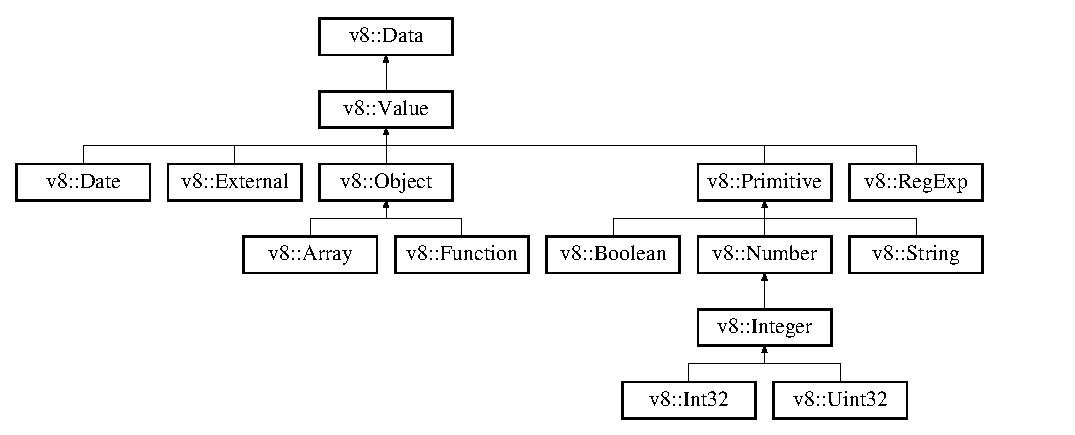
\includegraphics[height=11.837399cm]{classv8_1_1_value}
\end{center}
\end{figure}
\subsection*{Public Member Functions}
\begin{DoxyCompactItemize}
\item 
\hyperlink{classv8_1_1_value_ab7fe6f0f40ad56063af2b549d9c16938}{V8\+\_\+\+I\+N\+L\+I\+N\+E} (bool Is\+Undefined() const)
\item 
\hyperlink{classv8_1_1_value_a19bb214761816faf8b2784e4d78c9f21}{V8\+\_\+\+I\+N\+L\+I\+N\+E} (bool Is\+Null() const)
\item 
bool \hyperlink{classv8_1_1_value_a8f27462322186b295195eecb3e81d6d7}{Is\+True} () const 
\item 
bool \hyperlink{classv8_1_1_value_a68c0296071d01ca899825d7643cf495a}{Is\+False} () const 
\item 
\hyperlink{classv8_1_1_value_a14bd69255a9fd04fa641713188814958}{V8\+\_\+\+I\+N\+L\+I\+N\+E} (bool Is\+String() const)
\item 
bool \hyperlink{classv8_1_1_value_af3e6081c22d09a7bbc0a2aff59ed60a5}{Is\+Symbol} () const 
\item 
bool \hyperlink{classv8_1_1_value_a05532a34cdd215f273163830ed8b77e7}{Is\+Function} () const 
\item 
bool \hyperlink{classv8_1_1_value_aaee0b144087d20eae02314c9393ff80f}{Is\+Array} () const 
\item 
bool \hyperlink{classv8_1_1_value_a355b7991c5c978c0341f6f961b63c5a2}{Is\+Object} () const 
\item 
bool \hyperlink{classv8_1_1_value_a0aceb7645e71b096df5cd73d1252b1b0}{Is\+Boolean} () const 
\item 
bool \hyperlink{classv8_1_1_value_a1bd51e3e55f67c65b9a8f587fbffb7c7}{Is\+Number} () const 
\item 
bool \hyperlink{classv8_1_1_value_a7ac61a325c18af8dcb6d7d5bf47d2503}{Is\+External} () const 
\item 
bool \hyperlink{classv8_1_1_value_a01e1db51c65b2feace248b7acbf71a2c}{Is\+Int32} () const 
\item 
bool \hyperlink{classv8_1_1_value_a783c89631bac4ef3c4b909f40cc2b8d8}{Is\+Uint32} () const 
\item 
bool \hyperlink{classv8_1_1_value_a8bc11fab0aded4a805722ab6df173cae}{Is\+Date} () const 
\item 
bool \hyperlink{classv8_1_1_value_abe7bc06283e5e66013f2f056a943168b}{Is\+Boolean\+Object} () const 
\item 
bool \hyperlink{classv8_1_1_value_a5f4aa9504a6d8fc3af9489330179fe14}{Is\+Number\+Object} () const 
\item 
bool \hyperlink{classv8_1_1_value_a3e0f2727455fd01a39a60b92f77e28e0}{Is\+String\+Object} () const 
\item 
bool \hyperlink{classv8_1_1_value_a867baa94cb8f1069452359e6cef6751e}{Is\+Symbol\+Object} () const 
\item 
bool \hyperlink{classv8_1_1_value_a579fb52e893cdc24f8b77e5acc77d06d}{Is\+Native\+Error} () const 
\item 
bool \hyperlink{classv8_1_1_value_aae41e43486937d6122c297a0d43ac0b8}{Is\+Reg\+Exp} () const 
\item 
bool \hyperlink{classv8_1_1_value_a65f9dad740f2468b44dc16349611c351}{Is\+Array\+Buffer} () const 
\item 
bool \hyperlink{classv8_1_1_value_ac2f2f6c39f14a39fbb5b43577125dfe4}{Is\+Typed\+Array} () const 
\item 
bool \hyperlink{classv8_1_1_value_acbe2cd9c9cce96ee498677ba37c8466d}{Is\+Uint8\+Array} () const 
\item 
bool \hyperlink{classv8_1_1_value_ad3cb464ab5ef0215bd2cbdd4eb2b7e3d}{Is\+Uint8\+Clamped\+Array} () const 
\item 
bool \hyperlink{classv8_1_1_value_a10a88a2794271dfcd9c3abd565e8f28a}{Is\+Int8\+Array} () const 
\item 
bool \hyperlink{classv8_1_1_value_a4a45fabf58b241f5de3086a3dd0a09ae}{Is\+Uint16\+Array} () const 
\item 
bool \hyperlink{classv8_1_1_value_a928c586639dd75ae4efdaa66b1fc4d50}{Is\+Int16\+Array} () const 
\item 
bool \hyperlink{classv8_1_1_value_a5e39229dc74d534835cf4ceba10676f4}{Is\+Uint32\+Array} () const 
\item 
bool \hyperlink{classv8_1_1_value_a48eac78a49c8b42d9f8cf05c514b3750}{Is\+Int32\+Array} () const 
\item 
bool \hyperlink{classv8_1_1_value_a4effc7ca1a221dd8c1e23c0f28145ef0}{Is\+Float32\+Array} () const 
\item 
bool \hyperlink{classv8_1_1_value_a293f140b81b0219d1497e937ed948b1e}{Is\+Float64\+Array} () const 
\item 
\hypertarget{classv8_1_1_value_a73d653dc4a4999ce7258b40a4d8a1510}{}\hyperlink{classv8_1_1_local}{Local}$<$ \hyperlink{classv8_1_1_boolean}{Boolean} $>$ {\bfseries To\+Boolean} () const \label{classv8_1_1_value_a73d653dc4a4999ce7258b40a4d8a1510}

\item 
\hypertarget{classv8_1_1_value_a2706d2c0cf684a5179e76e8e404b3a5d}{}\hyperlink{classv8_1_1_local}{Local}$<$ \hyperlink{classv8_1_1_number}{Number} $>$ {\bfseries To\+Number} () const \label{classv8_1_1_value_a2706d2c0cf684a5179e76e8e404b3a5d}

\item 
\hypertarget{classv8_1_1_value_aef5739280886eb7a98ae0e98371dae39}{}\hyperlink{classv8_1_1_local}{Local}$<$ \hyperlink{classv8_1_1_string}{String} $>$ {\bfseries To\+String} () const \label{classv8_1_1_value_aef5739280886eb7a98ae0e98371dae39}

\item 
\hypertarget{classv8_1_1_value_acff61b07d724079dc3a90d3e3fd57cb3}{}\hyperlink{classv8_1_1_local}{Local}$<$ \hyperlink{classv8_1_1_string}{String} $>$ {\bfseries To\+Detail\+String} () const \label{classv8_1_1_value_acff61b07d724079dc3a90d3e3fd57cb3}

\item 
\hypertarget{classv8_1_1_value_af40feaf010e829f2cdb787eb975b941d}{}\hyperlink{classv8_1_1_local}{Local}$<$ \hyperlink{classv8_1_1_object}{Object} $>$ {\bfseries To\+Object} () const \label{classv8_1_1_value_af40feaf010e829f2cdb787eb975b941d}

\item 
\hypertarget{classv8_1_1_value_a3941f80b54b0707c6153657cc688ac93}{}\hyperlink{classv8_1_1_local}{Local}$<$ \hyperlink{classv8_1_1_integer}{Integer} $>$ {\bfseries To\+Integer} () const \label{classv8_1_1_value_a3941f80b54b0707c6153657cc688ac93}

\item 
\hypertarget{classv8_1_1_value_aed71590ec8bd5ef7972d7a0d844b2cd7}{}\hyperlink{classv8_1_1_local}{Local}$<$ \hyperlink{classv8_1_1_uint32}{Uint32} $>$ {\bfseries To\+Uint32} () const \label{classv8_1_1_value_aed71590ec8bd5ef7972d7a0d844b2cd7}

\item 
\hypertarget{classv8_1_1_value_adf5d2c0c0bf58d60f2401d8437df26b0}{}\hyperlink{classv8_1_1_local}{Local}$<$ \hyperlink{classv8_1_1_int32}{Int32} $>$ {\bfseries To\+Int32} () const \label{classv8_1_1_value_adf5d2c0c0bf58d60f2401d8437df26b0}

\item 
\hyperlink{classv8_1_1_local}{Local}$<$ \hyperlink{classv8_1_1_uint32}{Uint32} $>$ \hyperlink{classv8_1_1_value_ae810be0ae81a87f677592d0176daac48}{To\+Array\+Index} () const 
\item 
\hypertarget{classv8_1_1_value_a392d60e0ab58b5b13c0ac1e5b4b9f04b}{}bool {\bfseries Boolean\+Value} () const \label{classv8_1_1_value_a392d60e0ab58b5b13c0ac1e5b4b9f04b}

\item 
\hypertarget{classv8_1_1_value_a4634d525bae654cdc50c398bfaee11aa}{}double {\bfseries Number\+Value} () const \label{classv8_1_1_value_a4634d525bae654cdc50c398bfaee11aa}

\item 
\hypertarget{classv8_1_1_value_ac61c74a94dea10f48a64f5906b6dd43d}{}int64\+\_\+t {\bfseries Integer\+Value} () const \label{classv8_1_1_value_ac61c74a94dea10f48a64f5906b6dd43d}

\item 
\hypertarget{classv8_1_1_value_af25557359e6bb79436ed60df18703d66}{}uint32\+\_\+t {\bfseries Uint32\+Value} () const \label{classv8_1_1_value_af25557359e6bb79436ed60df18703d66}

\item 
\hypertarget{classv8_1_1_value_a24daae9d99d02ff2e24b60287dcd4d95}{}int32\+\_\+t {\bfseries Int32\+Value} () const \label{classv8_1_1_value_a24daae9d99d02ff2e24b60287dcd4d95}

\item 
bool \hyperlink{classv8_1_1_value_adc2a7a92a120675bbd4c992163a20869}{Equals} (\hyperlink{classv8_1_1_handle}{Handle}$<$ \hyperlink{classv8_1_1_value}{Value} $>$ that) const 
\item 
\hypertarget{classv8_1_1_value_abb564818715b818957adc97716a076ba}{}bool {\bfseries Strict\+Equals} (\hyperlink{classv8_1_1_handle}{Handle}$<$ \hyperlink{classv8_1_1_value}{Value} $>$ that) const \label{classv8_1_1_value_abb564818715b818957adc97716a076ba}

\item 
\hypertarget{classv8_1_1_value_ae2b6c816081fe138d077cb9c166ea6e7}{}{\footnotesize template$<$class T $>$ }\\{\bfseries V8\+\_\+\+I\+N\+L\+I\+N\+E} (static \hyperlink{classv8_1_1_value}{Value} $\ast$Cast(T $\ast$value))\label{classv8_1_1_value_ae2b6c816081fe138d077cb9c166ea6e7}

\end{DoxyCompactItemize}


\subsection{Detailed Description}
The superclass of all Java\+Script values and objects. 

\subsection{Member Function Documentation}
\hypertarget{classv8_1_1_value_adc2a7a92a120675bbd4c992163a20869}{}\index{v8\+::\+Value@{v8\+::\+Value}!Equals@{Equals}}
\index{Equals@{Equals}!v8\+::\+Value@{v8\+::\+Value}}
\subsubsection[{Equals}]{\setlength{\rightskip}{0pt plus 5cm}bool v8\+::\+Value\+::\+Equals (
\begin{DoxyParamCaption}
\item[{{\bf Handle}$<$ {\bf Value} $>$}]{that}
\end{DoxyParamCaption}
) const}\label{classv8_1_1_value_adc2a7a92a120675bbd4c992163a20869}
J\+S == \hypertarget{classv8_1_1_value_aaee0b144087d20eae02314c9393ff80f}{}\index{v8\+::\+Value@{v8\+::\+Value}!Is\+Array@{Is\+Array}}
\index{Is\+Array@{Is\+Array}!v8\+::\+Value@{v8\+::\+Value}}
\subsubsection[{Is\+Array}]{\setlength{\rightskip}{0pt plus 5cm}bool v8\+::\+Value\+::\+Is\+Array (
\begin{DoxyParamCaption}
{}
\end{DoxyParamCaption}
) const}\label{classv8_1_1_value_aaee0b144087d20eae02314c9393ff80f}
Returns true if this value is an array. \hypertarget{classv8_1_1_value_a65f9dad740f2468b44dc16349611c351}{}\index{v8\+::\+Value@{v8\+::\+Value}!Is\+Array\+Buffer@{Is\+Array\+Buffer}}
\index{Is\+Array\+Buffer@{Is\+Array\+Buffer}!v8\+::\+Value@{v8\+::\+Value}}
\subsubsection[{Is\+Array\+Buffer}]{\setlength{\rightskip}{0pt plus 5cm}bool v8\+::\+Value\+::\+Is\+Array\+Buffer (
\begin{DoxyParamCaption}
{}
\end{DoxyParamCaption}
) const}\label{classv8_1_1_value_a65f9dad740f2468b44dc16349611c351}
Returns true if this value is an \hyperlink{classv8_1_1_array_buffer}{Array\+Buffer}. This is an experimental feature. \hypertarget{classv8_1_1_value_a0aceb7645e71b096df5cd73d1252b1b0}{}\index{v8\+::\+Value@{v8\+::\+Value}!Is\+Boolean@{Is\+Boolean}}
\index{Is\+Boolean@{Is\+Boolean}!v8\+::\+Value@{v8\+::\+Value}}
\subsubsection[{Is\+Boolean}]{\setlength{\rightskip}{0pt plus 5cm}bool v8\+::\+Value\+::\+Is\+Boolean (
\begin{DoxyParamCaption}
{}
\end{DoxyParamCaption}
) const}\label{classv8_1_1_value_a0aceb7645e71b096df5cd73d1252b1b0}
Returns true if this value is boolean. \hypertarget{classv8_1_1_value_abe7bc06283e5e66013f2f056a943168b}{}\index{v8\+::\+Value@{v8\+::\+Value}!Is\+Boolean\+Object@{Is\+Boolean\+Object}}
\index{Is\+Boolean\+Object@{Is\+Boolean\+Object}!v8\+::\+Value@{v8\+::\+Value}}
\subsubsection[{Is\+Boolean\+Object}]{\setlength{\rightskip}{0pt plus 5cm}bool v8\+::\+Value\+::\+Is\+Boolean\+Object (
\begin{DoxyParamCaption}
{}
\end{DoxyParamCaption}
) const}\label{classv8_1_1_value_abe7bc06283e5e66013f2f056a943168b}
Returns true if this value is a \hyperlink{classv8_1_1_boolean}{Boolean} object. \hypertarget{classv8_1_1_value_a8bc11fab0aded4a805722ab6df173cae}{}\index{v8\+::\+Value@{v8\+::\+Value}!Is\+Date@{Is\+Date}}
\index{Is\+Date@{Is\+Date}!v8\+::\+Value@{v8\+::\+Value}}
\subsubsection[{Is\+Date}]{\setlength{\rightskip}{0pt plus 5cm}bool v8\+::\+Value\+::\+Is\+Date (
\begin{DoxyParamCaption}
{}
\end{DoxyParamCaption}
) const}\label{classv8_1_1_value_a8bc11fab0aded4a805722ab6df173cae}
Returns true if this value is a \hyperlink{classv8_1_1_date}{Date}. \hypertarget{classv8_1_1_value_a7ac61a325c18af8dcb6d7d5bf47d2503}{}\index{v8\+::\+Value@{v8\+::\+Value}!Is\+External@{Is\+External}}
\index{Is\+External@{Is\+External}!v8\+::\+Value@{v8\+::\+Value}}
\subsubsection[{Is\+External}]{\setlength{\rightskip}{0pt plus 5cm}bool v8\+::\+Value\+::\+Is\+External (
\begin{DoxyParamCaption}
{}
\end{DoxyParamCaption}
) const}\label{classv8_1_1_value_a7ac61a325c18af8dcb6d7d5bf47d2503}
Returns true if this value is external. \hypertarget{classv8_1_1_value_a68c0296071d01ca899825d7643cf495a}{}\index{v8\+::\+Value@{v8\+::\+Value}!Is\+False@{Is\+False}}
\index{Is\+False@{Is\+False}!v8\+::\+Value@{v8\+::\+Value}}
\subsubsection[{Is\+False}]{\setlength{\rightskip}{0pt plus 5cm}bool v8\+::\+Value\+::\+Is\+False (
\begin{DoxyParamCaption}
{}
\end{DoxyParamCaption}
) const}\label{classv8_1_1_value_a68c0296071d01ca899825d7643cf495a}
Returns true if this value is false. \hypertarget{classv8_1_1_value_a4effc7ca1a221dd8c1e23c0f28145ef0}{}\index{v8\+::\+Value@{v8\+::\+Value}!Is\+Float32\+Array@{Is\+Float32\+Array}}
\index{Is\+Float32\+Array@{Is\+Float32\+Array}!v8\+::\+Value@{v8\+::\+Value}}
\subsubsection[{Is\+Float32\+Array}]{\setlength{\rightskip}{0pt plus 5cm}bool v8\+::\+Value\+::\+Is\+Float32\+Array (
\begin{DoxyParamCaption}
{}
\end{DoxyParamCaption}
) const}\label{classv8_1_1_value_a4effc7ca1a221dd8c1e23c0f28145ef0}
Returns true if this value is a \hyperlink{classv8_1_1_float32_array}{Float32\+Array}. This is an experimental feature. \hypertarget{classv8_1_1_value_a293f140b81b0219d1497e937ed948b1e}{}\index{v8\+::\+Value@{v8\+::\+Value}!Is\+Float64\+Array@{Is\+Float64\+Array}}
\index{Is\+Float64\+Array@{Is\+Float64\+Array}!v8\+::\+Value@{v8\+::\+Value}}
\subsubsection[{Is\+Float64\+Array}]{\setlength{\rightskip}{0pt plus 5cm}bool v8\+::\+Value\+::\+Is\+Float64\+Array (
\begin{DoxyParamCaption}
{}
\end{DoxyParamCaption}
) const}\label{classv8_1_1_value_a293f140b81b0219d1497e937ed948b1e}
Returns true if this value is a \hyperlink{classv8_1_1_float64_array}{Float64\+Array}. This is an experimental feature. \hypertarget{classv8_1_1_value_a05532a34cdd215f273163830ed8b77e7}{}\index{v8\+::\+Value@{v8\+::\+Value}!Is\+Function@{Is\+Function}}
\index{Is\+Function@{Is\+Function}!v8\+::\+Value@{v8\+::\+Value}}
\subsubsection[{Is\+Function}]{\setlength{\rightskip}{0pt plus 5cm}bool v8\+::\+Value\+::\+Is\+Function (
\begin{DoxyParamCaption}
{}
\end{DoxyParamCaption}
) const}\label{classv8_1_1_value_a05532a34cdd215f273163830ed8b77e7}
Returns true if this value is a function. \hypertarget{classv8_1_1_value_a928c586639dd75ae4efdaa66b1fc4d50}{}\index{v8\+::\+Value@{v8\+::\+Value}!Is\+Int16\+Array@{Is\+Int16\+Array}}
\index{Is\+Int16\+Array@{Is\+Int16\+Array}!v8\+::\+Value@{v8\+::\+Value}}
\subsubsection[{Is\+Int16\+Array}]{\setlength{\rightskip}{0pt plus 5cm}bool v8\+::\+Value\+::\+Is\+Int16\+Array (
\begin{DoxyParamCaption}
{}
\end{DoxyParamCaption}
) const}\label{classv8_1_1_value_a928c586639dd75ae4efdaa66b1fc4d50}
Returns true if this value is an \hyperlink{classv8_1_1_int16_array}{Int16\+Array}. This is an experimental feature. \hypertarget{classv8_1_1_value_a01e1db51c65b2feace248b7acbf71a2c}{}\index{v8\+::\+Value@{v8\+::\+Value}!Is\+Int32@{Is\+Int32}}
\index{Is\+Int32@{Is\+Int32}!v8\+::\+Value@{v8\+::\+Value}}
\subsubsection[{Is\+Int32}]{\setlength{\rightskip}{0pt plus 5cm}bool v8\+::\+Value\+::\+Is\+Int32 (
\begin{DoxyParamCaption}
{}
\end{DoxyParamCaption}
) const}\label{classv8_1_1_value_a01e1db51c65b2feace248b7acbf71a2c}
Returns true if this value is a 32-\/bit signed integer. \hypertarget{classv8_1_1_value_a48eac78a49c8b42d9f8cf05c514b3750}{}\index{v8\+::\+Value@{v8\+::\+Value}!Is\+Int32\+Array@{Is\+Int32\+Array}}
\index{Is\+Int32\+Array@{Is\+Int32\+Array}!v8\+::\+Value@{v8\+::\+Value}}
\subsubsection[{Is\+Int32\+Array}]{\setlength{\rightskip}{0pt plus 5cm}bool v8\+::\+Value\+::\+Is\+Int32\+Array (
\begin{DoxyParamCaption}
{}
\end{DoxyParamCaption}
) const}\label{classv8_1_1_value_a48eac78a49c8b42d9f8cf05c514b3750}
Returns true if this value is an \hyperlink{classv8_1_1_int32_array}{Int32\+Array}. This is an experimental feature. \hypertarget{classv8_1_1_value_a10a88a2794271dfcd9c3abd565e8f28a}{}\index{v8\+::\+Value@{v8\+::\+Value}!Is\+Int8\+Array@{Is\+Int8\+Array}}
\index{Is\+Int8\+Array@{Is\+Int8\+Array}!v8\+::\+Value@{v8\+::\+Value}}
\subsubsection[{Is\+Int8\+Array}]{\setlength{\rightskip}{0pt plus 5cm}bool v8\+::\+Value\+::\+Is\+Int8\+Array (
\begin{DoxyParamCaption}
{}
\end{DoxyParamCaption}
) const}\label{classv8_1_1_value_a10a88a2794271dfcd9c3abd565e8f28a}
Returns true if this value is an \hyperlink{classv8_1_1_int8_array}{Int8\+Array}. This is an experimental feature. \hypertarget{classv8_1_1_value_a579fb52e893cdc24f8b77e5acc77d06d}{}\index{v8\+::\+Value@{v8\+::\+Value}!Is\+Native\+Error@{Is\+Native\+Error}}
\index{Is\+Native\+Error@{Is\+Native\+Error}!v8\+::\+Value@{v8\+::\+Value}}
\subsubsection[{Is\+Native\+Error}]{\setlength{\rightskip}{0pt plus 5cm}bool v8\+::\+Value\+::\+Is\+Native\+Error (
\begin{DoxyParamCaption}
{}
\end{DoxyParamCaption}
) const}\label{classv8_1_1_value_a579fb52e893cdc24f8b77e5acc77d06d}
Returns true if this value is a Native\+Error. \hypertarget{classv8_1_1_value_a1bd51e3e55f67c65b9a8f587fbffb7c7}{}\index{v8\+::\+Value@{v8\+::\+Value}!Is\+Number@{Is\+Number}}
\index{Is\+Number@{Is\+Number}!v8\+::\+Value@{v8\+::\+Value}}
\subsubsection[{Is\+Number}]{\setlength{\rightskip}{0pt plus 5cm}bool v8\+::\+Value\+::\+Is\+Number (
\begin{DoxyParamCaption}
{}
\end{DoxyParamCaption}
) const}\label{classv8_1_1_value_a1bd51e3e55f67c65b9a8f587fbffb7c7}
Returns true if this value is a number. \hypertarget{classv8_1_1_value_a5f4aa9504a6d8fc3af9489330179fe14}{}\index{v8\+::\+Value@{v8\+::\+Value}!Is\+Number\+Object@{Is\+Number\+Object}}
\index{Is\+Number\+Object@{Is\+Number\+Object}!v8\+::\+Value@{v8\+::\+Value}}
\subsubsection[{Is\+Number\+Object}]{\setlength{\rightskip}{0pt plus 5cm}bool v8\+::\+Value\+::\+Is\+Number\+Object (
\begin{DoxyParamCaption}
{}
\end{DoxyParamCaption}
) const}\label{classv8_1_1_value_a5f4aa9504a6d8fc3af9489330179fe14}
Returns true if this value is a \hyperlink{classv8_1_1_number}{Number} object. \hypertarget{classv8_1_1_value_a355b7991c5c978c0341f6f961b63c5a2}{}\index{v8\+::\+Value@{v8\+::\+Value}!Is\+Object@{Is\+Object}}
\index{Is\+Object@{Is\+Object}!v8\+::\+Value@{v8\+::\+Value}}
\subsubsection[{Is\+Object}]{\setlength{\rightskip}{0pt plus 5cm}bool v8\+::\+Value\+::\+Is\+Object (
\begin{DoxyParamCaption}
{}
\end{DoxyParamCaption}
) const}\label{classv8_1_1_value_a355b7991c5c978c0341f6f961b63c5a2}
Returns true if this value is an object. \hypertarget{classv8_1_1_value_aae41e43486937d6122c297a0d43ac0b8}{}\index{v8\+::\+Value@{v8\+::\+Value}!Is\+Reg\+Exp@{Is\+Reg\+Exp}}
\index{Is\+Reg\+Exp@{Is\+Reg\+Exp}!v8\+::\+Value@{v8\+::\+Value}}
\subsubsection[{Is\+Reg\+Exp}]{\setlength{\rightskip}{0pt plus 5cm}bool v8\+::\+Value\+::\+Is\+Reg\+Exp (
\begin{DoxyParamCaption}
{}
\end{DoxyParamCaption}
) const}\label{classv8_1_1_value_aae41e43486937d6122c297a0d43ac0b8}
Returns true if this value is a \hyperlink{classv8_1_1_reg_exp}{Reg\+Exp}. \hypertarget{classv8_1_1_value_a3e0f2727455fd01a39a60b92f77e28e0}{}\index{v8\+::\+Value@{v8\+::\+Value}!Is\+String\+Object@{Is\+String\+Object}}
\index{Is\+String\+Object@{Is\+String\+Object}!v8\+::\+Value@{v8\+::\+Value}}
\subsubsection[{Is\+String\+Object}]{\setlength{\rightskip}{0pt plus 5cm}bool v8\+::\+Value\+::\+Is\+String\+Object (
\begin{DoxyParamCaption}
{}
\end{DoxyParamCaption}
) const}\label{classv8_1_1_value_a3e0f2727455fd01a39a60b92f77e28e0}
Returns true if this value is a \hyperlink{classv8_1_1_string}{String} object. \hypertarget{classv8_1_1_value_af3e6081c22d09a7bbc0a2aff59ed60a5}{}\index{v8\+::\+Value@{v8\+::\+Value}!Is\+Symbol@{Is\+Symbol}}
\index{Is\+Symbol@{Is\+Symbol}!v8\+::\+Value@{v8\+::\+Value}}
\subsubsection[{Is\+Symbol}]{\setlength{\rightskip}{0pt plus 5cm}bool v8\+::\+Value\+::\+Is\+Symbol (
\begin{DoxyParamCaption}
{}
\end{DoxyParamCaption}
) const}\label{classv8_1_1_value_af3e6081c22d09a7bbc0a2aff59ed60a5}
Returns true if this value is a symbol. This is an experimental feature. \hypertarget{classv8_1_1_value_a867baa94cb8f1069452359e6cef6751e}{}\index{v8\+::\+Value@{v8\+::\+Value}!Is\+Symbol\+Object@{Is\+Symbol\+Object}}
\index{Is\+Symbol\+Object@{Is\+Symbol\+Object}!v8\+::\+Value@{v8\+::\+Value}}
\subsubsection[{Is\+Symbol\+Object}]{\setlength{\rightskip}{0pt plus 5cm}bool v8\+::\+Value\+::\+Is\+Symbol\+Object (
\begin{DoxyParamCaption}
{}
\end{DoxyParamCaption}
) const}\label{classv8_1_1_value_a867baa94cb8f1069452359e6cef6751e}
Returns true if this value is a \hyperlink{classv8_1_1_symbol}{Symbol} object. This is an experimental feature. \hypertarget{classv8_1_1_value_a8f27462322186b295195eecb3e81d6d7}{}\index{v8\+::\+Value@{v8\+::\+Value}!Is\+True@{Is\+True}}
\index{Is\+True@{Is\+True}!v8\+::\+Value@{v8\+::\+Value}}
\subsubsection[{Is\+True}]{\setlength{\rightskip}{0pt plus 5cm}bool v8\+::\+Value\+::\+Is\+True (
\begin{DoxyParamCaption}
{}
\end{DoxyParamCaption}
) const}\label{classv8_1_1_value_a8f27462322186b295195eecb3e81d6d7}
Returns true if this value is true. \hypertarget{classv8_1_1_value_ac2f2f6c39f14a39fbb5b43577125dfe4}{}\index{v8\+::\+Value@{v8\+::\+Value}!Is\+Typed\+Array@{Is\+Typed\+Array}}
\index{Is\+Typed\+Array@{Is\+Typed\+Array}!v8\+::\+Value@{v8\+::\+Value}}
\subsubsection[{Is\+Typed\+Array}]{\setlength{\rightskip}{0pt plus 5cm}bool v8\+::\+Value\+::\+Is\+Typed\+Array (
\begin{DoxyParamCaption}
{}
\end{DoxyParamCaption}
) const}\label{classv8_1_1_value_ac2f2f6c39f14a39fbb5b43577125dfe4}
Returns true if this value is one of Typed\+Arrays. This is an experimental feature. \hypertarget{classv8_1_1_value_a4a45fabf58b241f5de3086a3dd0a09ae}{}\index{v8\+::\+Value@{v8\+::\+Value}!Is\+Uint16\+Array@{Is\+Uint16\+Array}}
\index{Is\+Uint16\+Array@{Is\+Uint16\+Array}!v8\+::\+Value@{v8\+::\+Value}}
\subsubsection[{Is\+Uint16\+Array}]{\setlength{\rightskip}{0pt plus 5cm}bool v8\+::\+Value\+::\+Is\+Uint16\+Array (
\begin{DoxyParamCaption}
{}
\end{DoxyParamCaption}
) const}\label{classv8_1_1_value_a4a45fabf58b241f5de3086a3dd0a09ae}
Returns true if this value is an \hyperlink{classv8_1_1_uint16_array}{Uint16\+Array}. This is an experimental feature. \hypertarget{classv8_1_1_value_a783c89631bac4ef3c4b909f40cc2b8d8}{}\index{v8\+::\+Value@{v8\+::\+Value}!Is\+Uint32@{Is\+Uint32}}
\index{Is\+Uint32@{Is\+Uint32}!v8\+::\+Value@{v8\+::\+Value}}
\subsubsection[{Is\+Uint32}]{\setlength{\rightskip}{0pt plus 5cm}bool v8\+::\+Value\+::\+Is\+Uint32 (
\begin{DoxyParamCaption}
{}
\end{DoxyParamCaption}
) const}\label{classv8_1_1_value_a783c89631bac4ef3c4b909f40cc2b8d8}
Returns true if this value is a 32-\/bit unsigned integer. \hypertarget{classv8_1_1_value_a5e39229dc74d534835cf4ceba10676f4}{}\index{v8\+::\+Value@{v8\+::\+Value}!Is\+Uint32\+Array@{Is\+Uint32\+Array}}
\index{Is\+Uint32\+Array@{Is\+Uint32\+Array}!v8\+::\+Value@{v8\+::\+Value}}
\subsubsection[{Is\+Uint32\+Array}]{\setlength{\rightskip}{0pt plus 5cm}bool v8\+::\+Value\+::\+Is\+Uint32\+Array (
\begin{DoxyParamCaption}
{}
\end{DoxyParamCaption}
) const}\label{classv8_1_1_value_a5e39229dc74d534835cf4ceba10676f4}
Returns true if this value is an \hyperlink{classv8_1_1_uint32_array}{Uint32\+Array}. This is an experimental feature. \hypertarget{classv8_1_1_value_acbe2cd9c9cce96ee498677ba37c8466d}{}\index{v8\+::\+Value@{v8\+::\+Value}!Is\+Uint8\+Array@{Is\+Uint8\+Array}}
\index{Is\+Uint8\+Array@{Is\+Uint8\+Array}!v8\+::\+Value@{v8\+::\+Value}}
\subsubsection[{Is\+Uint8\+Array}]{\setlength{\rightskip}{0pt plus 5cm}bool v8\+::\+Value\+::\+Is\+Uint8\+Array (
\begin{DoxyParamCaption}
{}
\end{DoxyParamCaption}
) const}\label{classv8_1_1_value_acbe2cd9c9cce96ee498677ba37c8466d}
Returns true if this value is an \hyperlink{classv8_1_1_uint8_array}{Uint8\+Array}. This is an experimental feature. \hypertarget{classv8_1_1_value_ad3cb464ab5ef0215bd2cbdd4eb2b7e3d}{}\index{v8\+::\+Value@{v8\+::\+Value}!Is\+Uint8\+Clamped\+Array@{Is\+Uint8\+Clamped\+Array}}
\index{Is\+Uint8\+Clamped\+Array@{Is\+Uint8\+Clamped\+Array}!v8\+::\+Value@{v8\+::\+Value}}
\subsubsection[{Is\+Uint8\+Clamped\+Array}]{\setlength{\rightskip}{0pt plus 5cm}bool v8\+::\+Value\+::\+Is\+Uint8\+Clamped\+Array (
\begin{DoxyParamCaption}
{}
\end{DoxyParamCaption}
) const}\label{classv8_1_1_value_ad3cb464ab5ef0215bd2cbdd4eb2b7e3d}
Returns true if this value is an \hyperlink{classv8_1_1_uint8_clamped_array}{Uint8\+Clamped\+Array}. This is an experimental feature. \hypertarget{classv8_1_1_value_ae810be0ae81a87f677592d0176daac48}{}\index{v8\+::\+Value@{v8\+::\+Value}!To\+Array\+Index@{To\+Array\+Index}}
\index{To\+Array\+Index@{To\+Array\+Index}!v8\+::\+Value@{v8\+::\+Value}}
\subsubsection[{To\+Array\+Index}]{\setlength{\rightskip}{0pt plus 5cm}{\bf Local}$<${\bf Uint32}$>$ v8\+::\+Value\+::\+To\+Array\+Index (
\begin{DoxyParamCaption}
{}
\end{DoxyParamCaption}
) const}\label{classv8_1_1_value_ae810be0ae81a87f677592d0176daac48}
Attempts to convert a string to an array index. Returns an empty handle if the conversion fails. \hypertarget{classv8_1_1_value_ab7fe6f0f40ad56063af2b549d9c16938}{}\index{v8\+::\+Value@{v8\+::\+Value}!V8\+\_\+\+I\+N\+L\+I\+N\+E@{V8\+\_\+\+I\+N\+L\+I\+N\+E}}
\index{V8\+\_\+\+I\+N\+L\+I\+N\+E@{V8\+\_\+\+I\+N\+L\+I\+N\+E}!v8\+::\+Value@{v8\+::\+Value}}
\subsubsection[{V8\+\_\+\+I\+N\+L\+I\+N\+E}]{\setlength{\rightskip}{0pt plus 5cm}v8\+::\+Value\+::\+V8\+\_\+\+I\+N\+L\+I\+N\+E (
\begin{DoxyParamCaption}
\item[{bool Is\+Undefined()}]{const}
\end{DoxyParamCaption}
)}\label{classv8_1_1_value_ab7fe6f0f40ad56063af2b549d9c16938}
Returns true if this value is the undefined value. See E\+C\+M\+A-\/262 4.\+3.\+10. \hypertarget{classv8_1_1_value_a19bb214761816faf8b2784e4d78c9f21}{}\index{v8\+::\+Value@{v8\+::\+Value}!V8\+\_\+\+I\+N\+L\+I\+N\+E@{V8\+\_\+\+I\+N\+L\+I\+N\+E}}
\index{V8\+\_\+\+I\+N\+L\+I\+N\+E@{V8\+\_\+\+I\+N\+L\+I\+N\+E}!v8\+::\+Value@{v8\+::\+Value}}
\subsubsection[{V8\+\_\+\+I\+N\+L\+I\+N\+E}]{\setlength{\rightskip}{0pt plus 5cm}v8\+::\+Value\+::\+V8\+\_\+\+I\+N\+L\+I\+N\+E (
\begin{DoxyParamCaption}
\item[{bool Is\+Null()}]{const}
\end{DoxyParamCaption}
)}\label{classv8_1_1_value_a19bb214761816faf8b2784e4d78c9f21}
Returns true if this value is the null value. See E\+C\+M\+A-\/262 4.\+3.\+11. \hypertarget{classv8_1_1_value_a14bd69255a9fd04fa641713188814958}{}\index{v8\+::\+Value@{v8\+::\+Value}!V8\+\_\+\+I\+N\+L\+I\+N\+E@{V8\+\_\+\+I\+N\+L\+I\+N\+E}}
\index{V8\+\_\+\+I\+N\+L\+I\+N\+E@{V8\+\_\+\+I\+N\+L\+I\+N\+E}!v8\+::\+Value@{v8\+::\+Value}}
\subsubsection[{V8\+\_\+\+I\+N\+L\+I\+N\+E}]{\setlength{\rightskip}{0pt plus 5cm}v8\+::\+Value\+::\+V8\+\_\+\+I\+N\+L\+I\+N\+E (
\begin{DoxyParamCaption}
\item[{bool Is\+String()}]{const}
\end{DoxyParamCaption}
)}\label{classv8_1_1_value_a14bd69255a9fd04fa641713188814958}
Returns true if this value is an instance of the \hyperlink{classv8_1_1_string}{String} type. See E\+C\+M\+A-\/262 8.\+4. 

The documentation for this class was generated from the following file\+:\begin{DoxyCompactItemize}
\item 
deps/v8/include/v8.\+h\end{DoxyCompactItemize}

\chapter{Example Documentation}
\hypertarget{process_8cc-example}{}\section{process.\+cc}

\begin{DoxyCodeInclude}
\end{DoxyCodeInclude}
 
\hypertarget{shell_8cc-example}{}\section{shell.\+cc}
A simple shell that takes a list of expressions on the command-\/line and executes them.


\begin{DoxyCodeInclude}
\end{DoxyCodeInclude}
 
%--- End generated contents ---

% Index
\backmatter
\newpage
\phantomsection
\clearemptydoublepage
\addcontentsline{toc}{chapter}{Index}
\printindex

\end{document}
